\documentclass[table,usenames,dvipsnames,number=9 %your number in series
                ,series=renal, %series abbreviation
                ,isbn=978-607-8432-13-4, %add your isbn here
                ,url=http://www.uatx.edu/, %change for your book
	            ,output=long % long|short|inprep
	            %,blackandwhite
	            %,smallfont
	            %,draftmode
		     ]{langsciold}
                  %]{langscinew}
                  %  ]{langsci}
%             
%%%%%%%%%%%%%%%%%%%%%%%%%%
%   additional packages  %
%%%%%%%%%%%%%%%%%%%%%%%%%%
% put all additional commands you need in the
% following files. If you do not know what this might
% mean, you can safely ignore this section
%\usepackage[spanish]{babel}
%\usepackage[final]{microtype}
%\usepackage[activate={true,nocompatibility}
%,final
%,tracking=true
%,kerning=true
%,spacing=true
%,factor=1100
%,stretch=10
%,shrink=10]{microtype}
\usepackage{localmetadata}
\usepackage{localpackages}
\usepackage{localhyphenation}
\usepackage{localcommands}
%\usepackage[letter,cam,center]{crop}
\usepackage{amsmath,amssymb,amsfonts}
%\usepackage{fontspec}
\usepackage{xunicode}
\usepackage{xltxtra}
\usepackage{polyglossia}
\setdefaultlanguage{spanish}
\setotherlanguages{english}
\usepackage{graphicx}
\usepackage{float}
%\usepackage{color}
\usepackage{array}
\usepackage{supertabular}
\usepackage{hhline}
\makeatletter
\newcommand\arraybslash{\let\\\@arraycr}
\makeatother
\setlength\tabcolsep{1mm}
\renewcommand\arraystretch{1.3}
\newtheorem{theorem}{Theorem}
\hypersetup{colorlinks=true, linkcolor=blue, citecolor=blue, filecolor=blue, urlcolor=blue}
\newcommand\textstyleInternetLink[1]{{\textcolor{blue}{#1}}}
\newcommand\textstyleVisitedInternetLink[1]{{\textcolor[rgb]{0.5019608,0.0,0.0}{#1}}}
%\DisemulatePackage{setspace}
\usepackage{setspace}
%%%\singlespacing
%%\onehalfspacing
%\doublespacing
%%\setstretch{1.15}
\linespread{1.25}
\usepackage{hyphenat}
\usepackage[shortcuts]{extdash}
\usepackage{parskip}
\setlength{\parindent}{0pt}
\usepackage{colortbl}
\usepackage{booktabs}
\usepackage{tabu, longtable}
\usepackage{pdflscape}
\usepackage{multicol}
\usepackage{multirow}
\usepackage{rotating}
%\usepackage{slashbox}
\usepackage{url}
\usepackage{wallpaper}
\usepackage{supertabular}
\usepackage{tocloft}
%\usepackage{caption}
%\captionsetup[table]{name=Cuadro}
%\usepackage[usenames,dvipsnames]{color}
\usepackage{titlesec, blindtext, color}
%\usepackage[usenames,dvipsnames]{color}
\usepackage[]{tocbibind}
\usepackage{etoolbox}
\usepackage{fontspec}
%%%\setmainfont{Linux Libertine O}
\newfontfamily\quotefont{Linux Biolinum O}
%%\newfontfamily\quotefont{GillSansMTPro-Book}
\AtBeginEnvironment{quote}{\quotefont\small}
\AtBeginEnvironment{quotation}{\quotefont\small}

%\usepackage{tocloft} 
%\usepackage[subfigure]{tocloft}
%\usepackage[]{tocbibind}
%\usepackage{tocloft}
%\usepackage{fancyhdr}
\renewcommand{\cftdot}{} % remove dots of table of content
\renewcommand{\cfttoctitlefont}{\hfill\Large\bfseries\MakeUppercase} % change toc title to upper case
\renewcommand{\cftaftertoctitle}{\hfill}
%\renewcommand{\cftchapfont}{\MakeUppercase} % change chapter headings to uppercase
%\renewcommand{\cftchappresnum}{CAP.} % try to put "Chapter" in front of e.g."1. Introduction"
%\renewcommand{\cfttoctitlefont}{\hfil\bf} 
\titleformat{\chapter}[hang]{\centering\normalfont\large\bfseries}{}{0pt}{\large} % \scshape ?
\renewcommand\thesection{\arabic{section}}
\setlength{\cftchapnumwidth}{0pt}
\renewcommand\thechapter{}
\titlespacing*{\chapter}{11pt}{0pt}{11pt}
\parindent0em
%\makeatletter
%\renewcommand*\l@section{\bprot@dottedtocline{1}{0em}{2.3em}}% no indentation
%\renewcommand{\@pnumwidth}{3em}
%\renewcommand{\@tocrmarg}{4em}
%\makeatother
%\usepackage[tocbreaksstrict,tocflat]{tocstyle}
%\usetocstyle{standard}
%\settocfeature{raggedhook}{\raggedright}
%\makeatletter
%\renewcommand{\@pnumwidth}{3em}
%\renewcommand{\@tocrmarg}{4em}
%\makeatother
% \KOMAoptions{toc=flat} 
%\setcounter{secnumdepth}{0}
%\selecttocstyleoption{tocflat}
%\usepackage{blindtext}
%\pagestyle{fancy}
%%\usepackage{tocstyle}
%%\settocfeature{leaders}{\ \leaders\hrule\hfill}
\usepackage{epigraph}
%\usepackage{lmodern}
%\setlength\tabcolsep{1mm}
%%%\usepackage{booktabs}
\usepackage{enumitem}
% % % % % % % % % % % % % 
\renewcommand*{\chapterpagestyle}{scrheadings}
\newlist{Obs}{description}{1}
\setlist[Obs]{labelindent=0.1\parindent,leftmargin=0.1\parindent}

%%\addto\captionsenglish{%
%%	\renewcommand\tablename{Cuadro}
%%}
%%
%%\AtBeginDocument{%
%%	\renewcommand\tablename{Cuadro}
%%}

\hyphenation{Estado ciernes épo-cas res-ca-te Ca-ta-lo-ga-ción en-se-ñan-za-apren-di-za-je}

%\includeonly{chapters/p1.tex}
%\usepackage{marvosym}
\usepackage{wasysym}
\usepackage{fontspec,lineno}
%\defaultfontfeatures{Mapping=tex-text}
%\setmainfont{GaramondPremrPro}
%%\setsansfont{Adobe Garamond Pro}%{GillSansMTPro-Light}
%set the font size and leading
%\renewcommand{\normalsize}{\fontsize{12}{15}\selectfont}
%\defaultfontfeatures{Ligatures=TeX}
\setmainfont[Path=\fontpath,Mapping=tex-text,Scale=MatchLowercase,Style=TitlingCaps,Ligatures={NoRequired,NoCommon,NoContextual},PunctuationSpace=0,Numbers={OldStyle,Lining},Scale=1.0]
{GillSansMTPro-Book}
\defaultfontfeatures{Ligatures=TeX}
\newfontfamily{\liningmainfont}[Path=\fontpath,Numbers={OldStyle,Lining},Ligatures=TeX,Scale=MatchLowercase,Scale=0.8]{Book_Antiqua}
\newcommand*{\footnotemarkcolor}{lsRed}
\makeatletter
\renewcommand{\@makefnmark}{%
  \noindent
  \makebox[5pt][r]{\@textsuperscript{\color{\footnotemarkcolor}\normalfont\liningmainfont\@thefnmark}}%
}
%s\def\splitfootnoterule{\kern-3\p@ \hrule width 8cm \kern2.6\p@}
\makeatother
\renewcommand{\footnoterule}{\vspace*{-4pt}
  \noindent\rule{2.25in}{1pt}\vspace*{2pt}}
%\setmainfont[Mapping=tex-text,Style=TitlingCaps,Ligatures={Common}]{Garamond Premier Pro}
%\defaultfontfeatures{Renderer=Basic,Ligatures=TeX}
%\setmathsfont(Digits,Latin,Greek){GillSansMTPro-Light}
%\setmainfont{Adobe Garamond Pro}
%\setmainfont{Mapping=tex-text}{GillSansMTPro-Book}
%\setmainfont{Calibri}
%\setmainfont{ClarendonLTStd}
%\setmainfont[%Ligatures={TeX,Common},
        %PunctuationSpace=0,
        %Numbers={Monospaced,Lining}%,
       %\addfontfeatures{Numbers={Monospaced,Lining}} 
        %Numbers={Proportional},	
%            ]{GillSansMTPro}
%\usepackage{arev}
%\usepackage[scaled]{berasans}
%\renewcommand*\familydefault{\sfdefault}  %%  to be sans serif
%\usepackage[T1]{fontenc}
%\def\Tiny{ \font\Tinyfont = cmr10 at 3pt \relax  \Tinyfont}
%\usepackage{hyperref}
\pdfpagewidth=216 true mm
\pdfpageheight=279 true mm
%\setlength{\headheight}{1.5\baselineskip}
\usepackage{multirow}
\usepackage{bigstrut}
%\usepackage{microtype}
%\DisableLigatures[f]{encoding = *, family = * }
\usepackage[hang,flushmargin,splitrule,multiple]{footmisc}% http://ctan.org/pkg/footmisc
\usepackage{relsize}% http://ctan.org/pkg/relsize
\renewcommand\footnotelayout{\footnotesize}
\renewcommand{\thefootnote}{\small\arabic{footnote}}%
%\makeatletter
%\renewcommand\@makefntext[1]{\leftskip=2em\hskip-2em\@makefnmark#1}
%\makeatother
%%\usepackage{scrextend}
%%\deffootnote[1em]{1.5em}{1em}{\textsuperscript{\thefootnotemark}}
%\renewcommand{\footnotemargin}{1em}
%\newcommand{\fn}[1]{\footnote{\hangpara{3em}{1} #1}}
\renewcommand{\hangfootparindent}{1.5em}% Indentation for 2nd etc. paragraphs in footnotes which cosists of more than one paragraph
\renewcommand{\hangfootparskip}{3pt}% Vertical space between paragraphs in multiparagraph footnotes
\renewcommand{\footnotemargin}{0.00001pt}% Setting left margin; this is the smallest value I can get to have second etc. lines indented to footnote number; zero put indentation to some positive value, and negative values do not help actually
\renewcommand{\footnotelayout}{\hspace{1.5em}}% Here you can modify the spacing between the footnote number and the text of footnote; keep this value and \hangfootparindent value the same
%\usepackage{fixltx2e}
%\renewcommand{\allcapsspacing}[1]{{\addfontfeature{LetterSpace=20.0}#1}}
%\renewcommand{\smallcapsspacing}[1]{{\addfontfeature{LetterSpace=5.0}#1}}
%\renewcommand{\textsc}[1]{\smallcapsspacing{\textsmallcaps{#1}}}
%\renewcommand{\smallcaps}[1]{\smallcapsspacing{\scshape\MakeTextLowercase{#1}}}
%\renewcommand{\rmdefault}{pplx}
%
%\XeTeXinterchartokenstate=1
%\chardef\CharNormal=0
%\chardef\CharBound=255
%\newXeTeXintercharclass\CharNumbers
%\XeTeXcharclass`0=\CharNumbers
%\XeTeXcharclass`1=\CharNumbers
%\XeTeXcharclass`2=\CharNumbers
%\XeTeXcharclass`3=\CharNumbers
%\XeTeXcharclass`4=\CharNumbers
%\XeTeXcharclass`5=\CharNumbers
%\XeTeXcharclass`6=\CharNumbers
%\XeTeXcharclass`7=\CharNumbers
%\XeTeXcharclass`8=\CharNumbers
%\XeTeXcharclass`9=\CharNumbers
%\newtoks\TokSetfont
%\TokSetfont={\begingroup\fontspec{\XeTeXinterchartokenstate=1
%\chardef\CharNormal=0
%\chardef\CharBound=255
%\newXeTeXintercharclass\CharNumbers
%\XeTeXcharclass`0=\CharNumbers
%\XeTeXcharclass`1=\CharNumbers
%\XeTeXcharclass`2=\CharNumbers
%\XeTeXcharclass`3=\CharNumbers
%\XeTeXcharclass`4=\CharNumbers
%\XeTeXcharclass`5=\CharNumbers
%\XeTeXcharclass`6=\CharNumbers
%\XeTeXcharclass`7=\CharNumbers
%\XeTeXcharclass`8=\CharNumbers
%\XeTeXcharclass`9=\CharNumbers
%\newtoks\TokSetfont
%\TokSetfont={\begingroup\fontspec{Latin Modern Mono}}
%\XeTeXinterchartoks\CharNormal\CharNumbers=\TokSetfont
%\XeTeXinterchartoks\CharBound\CharNumbers=\TokSetfont
%\XeTeXinterchartoks\CharNumbers\CharNormal={\endgroup}
%\XeTeXinterchartoks\CharNumbers\CharBound={\endgroup}}}
%\XeTeXinterchartoks\CharNormal\CharNumbers=\TokSetfont
%\XeTeXinterchartoks\CharBound\CharNumbers=\TokSetfont
%\XeTeXinterchartoks\CharNumbers\CharNormal={\endgroup}
%\XeTeXinterchartoks\CharNumbers\CharBound={\endgroup}
\newcommand{\lnt}[1]%
           {{\addfontfeatures{Numbers={Monospaced,Lining}}#1}}
\usepackage{tabulary}
\usepackage{textcomp}
%\usepackage[osf]{libertine}
%\usepackage{amsmath, amsthm}
%\usepackage[cmintegrals, cmbraces, libertine]{newtxmath}
%\usepackage[version=3]{mhchem}
\usepackage{amsmath} % must precede mathspec
%\usepackage[MnSymbol]{mathspec}
\usepackage{gillsans}
\usepackage[   %% --- EulerVM (MATH)
  small,       %for smaller Fonts
 euler-digits % digits in euler fonts style
]{eulervm}
%\usepackage{xtab}
%\renewcommand{\rmdefault}{pmnj}
\usepackage[framemethod=TikZ]{mdframed}
\usepackage{framed}
\usepackage{calc}
\usepackage[autostyle=true,babel,spanish=spanish,english=american,french=guillemets]{csquotes}
\usepackage{polyglossia}
\setdefaultlanguage{spanish}
%\usepackage{color}
%\usepackage[table]{xcolor}
\usepackage{array}
\usepackage{hhline}
%\usepackage{hyperref}
\hypersetup{colorlinks=true, linkcolor=blue, citecolor=blue, filecolor=blue, urlcolor=blue}
%\usepackage[lining]{ebgaramond}
%\usepackage{parskip}
\addtokomafont{disposition}{\rmfamily}
%%\setmonofont{LucidaSansTypewriterStd}
%%\setsansfont{GillSansMT}
\setlength{\headheight}{1.1\baselineskip}
\usepackage{pdfpages}
\usepackage{shapepar}
\usepackage{fixltx2e}
%\oldstylenums{1234567890}
%\renewcommand{\linenumberfont}{\scriptsize\addfontfeatures{Numbers={Lining, Monospaced}}}
%%%%%%%%%%%%%%%%%%%%%%%%%%%%%%%%%%%%%%%%%%%%%%%%
%%%             BEGIN DOCUMENT                   %%%
%%%%%%%%%%%%%%%%%%%%%%%%%%%%%%%%%%%%%%%%%%%%%%%%%%%%
\begin{document}
%\clearpage\setcounter{page}{9}
\pagenumbering{roman}
%\includepdf[pages={1}]{portada.pdf}
%\include{PagLegal}
\markboth{}{}
\thispagestyle{empty}
\maketitle
\frontmatter
%
\clearpage\setcounter{page}{7}
% %% uncomment if you have preface and/or acknowledgements
%\chapter*{Preface}
% \include{chapters/preface}
% \section*{Acknowledgements}
% \include{chapters/acknowledgements} 
\renewcommand{\cftpartleader}{\cftdotfill{\cftdotsep}} 
\renewcommand{\cftchapleader}{\cftdotfill{\cftdotsep}} 
\renewcommand{\cftsecleader}{\cftdotfill{\cftdotsep}}
\renewcommand{\cftdot}{$\ldots$}
\renewcommand{\contentsname}{Índice} % change "Contents" to "ÍNDICE"
\titlepage
\addtocontents{toc}{\bfseries {\,} \hfill Pág.\par} % add underlined "Chapter" and "page" before actually contents show up.
\newcommand*\NewPage{\newpage\null\thispagestyle{empty}\newpage}
%\renewcommand{\headrulewidth}{2pt}
%\renewcommand{\cftdot}{}
%%\renewcommand{\cfttoctitlefont}{\hfill\Large\bfseries\sffamily}
%%\renewcommand{\cftaftertoctitle}{\hfill}
%%\renewcommand{\cftaftertoctitleskip}{2.5cm}
%%\renewcommand{\cftbeforetoctitleskip}{2.5cm}
%%\renewcommand{\cftloftitlefont}{\hfill\Large\bfseries\sffamily}
%%\renewcommand{\cftafterloftitle}{\hfill \hfill
%\renewcommand{\cftafterloftitle}{\hfill \hfill \hfill
%%\\[3\baselineskip]{Figure No \hfill Title \hfill Page \linebreak} \vskip-50pt}
%%\renewcommand{\cftbeforeloftitleskip}{2.5cm}
%%\renewcommand{\cftlottitlefont}{\hfill\Large\bfseries\sffamily}
%%\renewcommand{\cftafterlottitle}{\hfill \hfill
%\renewcommand{\cftafterlottitle}{\hfill \hfill\hfill
%%\\[3\baselineskip]{Table No \hfill Title \hfill Page \linebreak }
%%\vskip-50pt}
%%\renewcommand{\cftbeforelottitleskip}{2.5cm}
%%\newlistof{appendices}{loa}{List of Appendices}
%%\renewcommand{\cftloatitlefont}{\hfill\Large\bfseries\sffamily}
%%\renewcommand{\cftafterloatitle}{\hfill \hfill
%\renewcommand{\cftafterloatitle}{\hfill \hfill\hfill
%%\\[3\baselineskip]{Appendix \hfill Title \hfill Page \linebreak}
%%\vskip-60pt}
%%\renewcommand{\cftbeforeloatitleskip}{2.5cm}
%%\renewcommand{\cftchappresnum}{Chapter }
%%\renewcommand{\cftchapaftersnum}{}
%%\renewcommand{\cftchapaftersnumb}{\qquad\quad\,\,}
%%\renewcommand{\cftsecpresnum}{\qquad\quad\,\,\,\, }
%%\renewcommand{\cftsubsecpresnum}{\quad\,\, }
%%\renewcommand{\cftsecaftersnum}{}
%%\renewcommand{\cftsecaftersnumb}{\qquad\qquad\,}
%%\renewcommand{\cftsubsecaftersnumb}{\quad}
% % % % % % % % % % % % % % % % % % % % % % %

\tableofcontents %

%\hrulefill %

\mainmatter %

%%%%%%%%%%%%%%%%%%%%%%%%%%%%%%%
%%%             Chapters                         %%%
%%%%%%%%%%%%%%%%%%%%%%%%%%%%%%%
%\documentclass{article}
%\usepackage{amsmath,amssymb,amsfonts}
%\usepackage{fontspec}
%\usepackage{xunicode}
%\usepackage{xltxtra}
%\usepackage{polyglossia}
%\setdefaultlanguage{spanish}
%\usepackage{color}
%\usepackage{array}
%\usepackage{hhline}
%\usepackage{hyperref}
%\hypersetup{colorlinks=true, linkcolor=blue, citecolor=blue, filecolor=blue, urlcolor=blue}
%\newtheorem{theorem}{Theorem}
\pagenumbering{arabic}
\clearpage\setcounter{page}{1}
\thispagestyle{empty}
\phantomsection{}
\addcontentsline{toc}{chapter}{Introducción\newline $\diamond$
\normalfont\textit{Elva Rivera Gómez}}
{\centering \large {\scshape\ Introducción}\newline {\itshape\ La enseñanza de la Historia y las opciones terminales\newline en las Licenciaturas en Historia en México\/}\par}
\markboth{la formación del historiador}{introducción}
\setcounter{footnote}{0}

\bigskip
\begin{center}
{\bfseries Elva Rivera Gómez\par}
\end{center}

\bigskip
\epigraph{¿Cómo se forman los historiadores? ¿Para qué se estudia la licenciatura en 
Historia en la Universidad? [\ldots] Tanto la formación como la información
del futuro historiador se orienta mucho más hacia la investigación 
que hacia la docencia, pese a que, por el contrario, 
el terreno de la práctica profesional es mucho 
más amplio en la enseñanza escolar.}{\itshape\ \textemdash{} Andrea Sánchez Quintanar\/}
\enlargethispage{2\baselineskip}

\bigskip
Por los pasillos de las licenciaturas en Historia, un fantasma atraviesa la enseñanza de la disciplina: 
 el fantasma de las competencias diseñadas por el mercado neoliberal. 

En las universidades mexicanas la enseñanza de la Historia como disciplina estuvo fuertemente orientada a la investigación, al menos durante la segunda mitad del siglo XX.\ La mayoría de las licenciaturas fundadas durante este periodo tomaron como
modelo el plan de estudios de la UNAM.\ Por ejemplo, las carreras de Historia
que se fundaron en 1945 en el Instituto de Historia de la Universidad Nacional Autónoma de México y en la casa de España, hoy Colegio de México, y la que se estableció en 1957 en la Universidad Iberoamericana. Mientras que en 1965 se fundó el Colegio de Historia en la Escuela de Filosofía y Letras de la Universidad Autónoma de Puebla. La UNAM inauguró la modalidad de enseñanza abierta en 1972, y  no fue sino hasta 1977 que la licenciatura en Historia se empezó a ofrecer por esta vía. Más tarde, en la década de los $80$,
algunas licenciaturas se fueron decantando por un modelo híbrido entre el plan de estudios de la UNAM y el de la UAM\@.

Si las y los historiadores\slash{}as son quienes conocen el saber-hacer de la disciplina, ¿qué ha pasado en la enseñanza, la investigación y la difusión, en el
diseño de los planes y programas de estudios a lo largo de los últimos treinta años? ¿Cómo se forma a los futuras generaciones de profesionales de la Historia, qué áreas formativas del perfil profesional son reconocidas en el mercado laboral de las y los egresados? Estas son algunas de las interrogantes que necesitamos responder hoy por hoy en la academia. 

\enlargethispage{1\baselineskip}
Algún barrunto de respuesta a estas preguntas seguramente lo encontraremos en los objetivos y el perfil de egreso de los planes y programas de estudio de nuestras carreras. Empero, si deseamos preservar los rasgos característicos de un perfil disciplinar consistente, es importante
enseñar a construir el conocimiento, a elaborarlo, a descubrirlo, a
resolver problemas, como alguna vez lo sugirió  Andrea Sánchez Quintanar (1996), quien también reconoció que los problemas a que se enfrentan tanto los\slash{}as historiadores\slash{}as que enseñan, como los\slash{}as que aprenden, abarcan un abanico tal que 

\begin{quote}
(\ldots) desde el abordaje filosófico de la disciplina \textemdash{}el por qué y para qué de la historia\textemdash{}; los diversos aspectos epistemológicos{} \textemdash{}las formas de
construcción del conocimiento histórico; las diversas teorías de la
historia y los métodos que las teorías implican; su aplicación a las áreas
específicas del conocimiento histórico y, por último, su elaboración y
formulación en un estructura formal orgánicamente estructurada, y con una
forma de expresión al menos clara o, si es posible, estéticamente valiosa
(\textit{ibid.}).
\end{quote}
\enlargethispage{1\baselineskip}
Sánchez Quintanar sustentó estas propuestas al revisar el
Plan de Estudios de Historia de la UNAM, que en ese entonces sólo contemplaba
dos cursos de didáctica de la historia. Desde su punto de vista, en estas
materias se debían estudiar los problemas que plantea la enseñanza de la
historia, tales como:

\begin{quotation}
(\ldots) problemas de organización educativa, elementos de sociología de la
educación, los problemas específicos de la transmisión-difusión del
conocimiento histórico (temporalidad, espacialidad y varios más) y, desde
luego, los propiamente didácticos: formulación de objetivos, técnicas
didácticas, proyectos de trabajo docente, programas y planes de estudio,
etcétera (\textit{ibid.}).
\end{quotation}

Estas reflexiones de Sánchez Quintanar se hicieron en el contexto de la UNAM,
justo cuando a nivel internacional se discutían los problemas referentes a
la enseñanza de la historia en Europa e Iberoamérica, y cuando en la
mayoría de las universidades estatales se iniciaban las reformas de los planes y programas 
 de estudio sugeridas por las políticas educativas neoliberales.

En el contexto internacional, tanto en Europa como  en Latinoamérica se
abordó la discusión sobre la formación del profesorado, y se propusieron un conjunto de
competencias para la enseñanza de la historia. A este respecto, Joan Pagés nos relata de que modo el Consejo de Europa se interesó por la enseñanza de la Historia, pues a finales de la década de los 90 se organizaron tres seminarios destinados a la reflexión sobre la formación inicial del profesorado de historia: en Viena (1998), Praga (1999) y Atenas
(2000). El objetivo central de tales eventos fue <<Aprender y enseñar la historia de Europa del siglo XX>>. 
De estas reuniones surgió una \textit{recomendación} relativa a la enseñanza de la historia en Europa en el siglo XXI (Pagés 2004, p. 163).

Para el caso iberoamericano, la Organización de Estados Iberoamericanos, a partir del Nodo Coordinador de la Cátedra de Historia de Iberoamérica, propuso 

\begin{quotation}
(\ldots) la necesidad de combinar la formación del profesorado de
historia con la formación para poder enseñar Historia de Iberoamérica,
haciendo hincapié en los valores y las competencias académicas y pedagógicas,
cuyas bases se apoyen en el sentido humanista, las experiencias comunes de los procesos históricos y el aprendizaje autónomo:

Unos valores y unas actitudes proclives a esta enseñanza basada en la
comprensión del otro, en la solidaridad y en la responsabilidad hacia un
pasado común y hacia un futuro en el que sean posibles los procesos de la
integración regional.

Unas competencias académicas referidas a la Historia en general y a la
Historia de Iberoamérica en particular, a sus rasgos específicos y a las
experiencias comunes de los procesos históricos que en ella se han
producido.

Unas competencias pedagógicas-didácticas facilitadoras de proceso de
aprendizaje autónomos, que permitan al profesor conocer, seleccionar,
utilizar, evaluar y desarrollar estrategias de intervención didáctica
(Pagés 2004, pp. 164\textendash{}165).
\end{quotation}
\enlargethispage{1\baselineskip}
Además, es importante señalar que se diseñaron las competencias académicas y
pedagógicas relacionadas con la naturaleza y el procedimiento del conocimiento histórico, consistentes en:

\begin{quotation}
(\ldots) las principales tendencias historiográficas y su evolución; el tipo de conceptos, datos y hechos que utiliza la Historia y el carácter relativista
de su interpretación; la comprensión y orientación en los sistemas temporal
y espacial; la comprensión del sentido procesal de la Historia, etcétera.
Por su parte las competencias pedagógicas las clasifican en tres grandes
grupos: la adquisición de las competencias sociales y de comunicación; la
concepción, planificación y programación de la actividad docente y la
organización, dirección y evaluación del proceso de enseñanza-aprendizaje
(\textit{ibid.}).
\end{quotation}

En este contexto internacional e iberoamericano de la década de los 
$90$, fue
que se empiezan a introducir en México nuevas reformas a los planes y programas de
estudio, y, paulatinamente, a transformarse el curriculum en las Licenciaturas en Historia 
de las universidades estatales. Entre otras cosas, se trataba de que ahora el curriculum se hiciera
flexible, que contará con un sistema de créditos, y que incluyera las opciones terminales.

Finalmente, en la primera década del siglo XXI, el Proyecto Tuning del año
2001 constituyó un espacio de reflexión sobre la educación superior, y
fue el marco para que en la IV Reunión de Seguimiento del Espacio Común de
Enseñanza Superior de la Unión Europea, América Latina y el Caribe (UEALC),
en octubre de 2002, se propusiera un proyecto para América Latina, el cual fue
presentado ante la Comisión Europea en el 2003. Un año más tarde surgió el
Proyecto ALFATuning-América Latina (2004\textendash{}2008).

\enlargethispage{1\baselineskip}
Los objetivos de este proyecto fueron, entre otros:

\begin{Obs}
\begin{sloppypar}
\item[$\bullet$] Contribuir al desarrollo de titulaciones fácilmente comparables y
comprensibles en una forma articulada en toda América Latina.
\end{sloppypar}

\item[$\bullet$] Impulsar a escala latinoamericana, un importante nivel de convergencia de la
educación superior en doce áreas temáticas, \textemdash{}entre éstas Historia\textemdash{}
mediante las definiciones aceptadas en común de resultados profesionales y
de aprendizajes.
\item[$\bullet$] Desarrollar perfiles profesionales en términos de competencias genéricas y
relativas a cada área de estudios incluyendo destrezas,\linebreak conocimientos y
contenido en las cuatro áreas temáticas del proyecto.
\item[$\bullet$] Desarrollar e intercambiar información relativa al desarrollo de los
currículos en las áreas seleccionadas y crear una estructura curricular
modelo expresada por puntos de referencia para cada área, promoviendo el
reconocimiento y la integración latinoamericana de titulaciones (Tuning
2004\textendash{}2008).
\end{Obs}

El Proyecto Tuning para América Latina (2004\textendash{}2008) señalaba cuatro líneas de
trabajo: (1) Competencias (genéricas y específicas), (2) Enfoques de
enseñanza, aprendizaje y evaluación, (3) Créditos académicos, y (4) Calidad
de los programas. La tercera, especialmente, propuso el trabajo del alumnado,
el sistema de créditos académicos, es decir, una medida que incidía directamente en la duración de los estudios del alumnado en el nivel superior.

Este antecedente internacional fue el marco referencial para que en las
diversas licenciaturas en Historia de las universidades mexicanas se
llevaran a cabo revisiones y reformas a los planes y programas de estudio
de esta disciplina. Para ese proceso ha sido central la evaluación y
acreditación de las carreras \textemdash{}ahora llamados Programas Educativos (PE)\textemdash{}, 
lo que ha obligado a confirmar y reconfirmar la calidad y pertinencia educativa de las licenciaturas. Asimismo, los organismos evaluadores (CIEES) y acreditadores
(COPAES) reconocidos por la Secretaría de Educación Pública, en sus
recomendaciones de evaluación, sugirieron que para llevar a cabo reformas a
los planes y programas se debían considerar los estudios y\slash{}o diagnósticos
del mercado laboral de la disciplina de historia. Para ellos,  la
opinión de los empleadores y de los egresadas\slash{}os, por una parte, era decisiva. Por la otra, la Secretaría de Educación Pública diseñó directrices sustentadas en los acuerdos de la Conferencia Mundial de Educación Superior (1989), el plan 
Bolonia y el proyecto Tuning, a fin de introducir el modelo 
de las competencias genéricas, disciplinares y profesionales en el diseño de los planes y programas de estudio.

Este nuevo escenario condujo a una transformación, en algunos casos parcial,
de los planes y programas de estudio de las licenciaturas en Historia. A las llamadas asignaturas y\slash{}o materias se les denominó a partir de entonces
Unidades de Aprendizaje, y se puso especial atención a las opciones y\slash{}o
áreas terminales de la carrera.

\enlargethispage{1\baselineskip}
En un trabajo reciente, Sebastián Plá señala que en la enseñanza de la historia 
como objeto de investigación en México,  a pesar de la falta de
conceptualización,  es notorio el reconocimiento como parte constitutiva de la identidad del
historiador  (Plá 2012, p. 166).  Este autor reconoce que, aunque los planes y programas de estudios sigan orientados esencialmente a la formación en la investigación,  la inserción laboral real de los\slash{}as egresados\slash{}as en Historia da fe de que estos planes y programas también ofrecen opciones en otras vertientes del conocimiento relacionadas con el quehacer del historiador\slash{}a, como la docencia y el patrimonio histórico. En ese mismo tenor, también son reveladoras las cifras del Observatorio Laboral de la Secretaría del Trabajo y Previsión Social (STPS) relativas a la inserción laboral de los\slash{}as egresados\slash{}as de Historia, que el mismo Plá nos trae a colación: 

\begin{quotation}
(\ldots) el 20.7\,\% de los egresados de las licenciaturas en Historia son maestros de secundaria, 4.9\,\% trabaja dando clases en bachillerato y 9.9\,\% como docentes universitarios, es decir, un poco más de la tercera parte de los
historiadores\slash{}as no se dedican a la investigación sino a la docencia, y una
cuarta parte lo hace lejos de los ambientes universitarios (\textit{ibid.}, p.
166).
\end{quotation}

Al reflexionar en torno a la dicotomía investigación\slash{}docencia, Plá reconoce que ésta se encuentra disociada o tiene poca relevancia en la formación del\slash{}a historiador\slash{}a en los planes y programas de estudio de las respectivas licenciaturas de las universidades mexicanas. Además, en un análisis sucinto expone cual es el lugar que ocupa el \textit{área de docencia} en algunas licenciaturas, encontrando, por ejemplo, algunas donde apenas se le asignan dos o tres asignaturas, como didáctica, enseñanza o docencia de la historia. Plá subraya, más adelante, que son varios los casos en los que estas asignaturas se engarzan con opciones terminales que abarcan otras temáticas, 
 como aprendizajes de la historia, instrumentos de evaluación y habilidades docentes (\textit{ibid.},~p.~167).

Así, pues, en la primera década del siglo XXI se han institucionalizado, a
partir de las reformas y de los estudios del mercado laboral \textemdash{}de
empleadores y egresados\textemdash{}, las áreas terminales y\slash{}o de especialización.
Éstas, según los perfiles de egreso, se orientan a la inserción en el
mercado laboral, cubriendo principalmente tres rubros: investigación, docencia y difusión. A continuación citaré sólo unos cuantos casos significativos, ya que este tema amerita un estudio más detallado que comprenda a todos los planes y programas de las carreras de Historia en el país, tanto de las universidades públicas como de las privadas.

Un primer ejemplo lo tenemos en las cuatro áreas de especialización que contempla la Licenciatura en Historia de la Universidad de Sonora:\linebreak (1)
\textit{Investigación histórica}, que incluye las subáreas de: (a) Historia
económica, (b) Historiografía,  (c) Historia cultural, (d) Historia política,
(e) Historia social, (f) Historia colonial, (g) Historia de las comunidades
étnicas; (2) \textit{Divulgación histórica}, que incorpora la enseñanza de
cursos referentes a la Producción y realización fotográfica I y II,
Producción y realización radiofónica I y II, Producción y realización
audiovisual I y II, Producción y realización de medios impresos I y II, y
Producción multimedia I y II;\ (3) \textit{Formación docente}, la cual abarca las
asignaturas de Políticas educativas, Administración educativa, Desarrollo
curricular, Sociología de la educación, Historia de la educación y
Multimedia educativa; y (4) \textit{Organización y administración de
archivos}, que integra los cursos de Taller de organización y
administración de archivos, Archivística y Producción multimedia I y II\@.

En tanto que la carrera de Historia de la Universidad de Guadalajara ofrece
las áreas de formación especializante en \textit{Historia y Comunicación},
\textit{Historia del Arte}, \textit{Prehistoria y Estudios Mesoamericanos},
\textit{Estudios Coloniales}, \textit{Historia Moderna de México}, y
\textit{Docencia en Historia}.

\enlargethispage{1\baselineskip}
Mientras que la Universidad de Autónoma de Nuevo León, en la Licenciatura en
Historia y Estudios en Humanidades, incluye el área de
\textit{Investigación}: Metodología de la investigación, Seminario de
Investigación (10º semestre); el área de \textit{Patrimonio y gestión
cultural}: Metodología de la difusión histórica (6º semestre), Patrimonio y
gestión cultural (7º semestre), Producción editorial (10º semestre); y 
el área de \textit{Docencia}, en la cual se insertan los contenidos de Teorías
del aprendizaje (6º semestre), Metodología de la enseñanza de la historia
(7º semestre) y Programación didáctica (10º semestre). En el octavo semestre se 
cursa Protocolo de investigación, y se realiza el servicio social (16~créditos); 
mientras que en el noveno semestre el alumnado tiene libre elección con 22 créditos.

Por su parte, la Licenciatura en Historia de la BUAP, en el plan de estudios
2009 (MUM), incluye las áreas terminales de \textit{Investigación} (Seminario
metodológico, Seminario de Investigación Histórica I y II y Seminario de
Tesis con un total de 16 créditos); \textit{Docencia} (Didáctica de la
Historia, Metodología de la Enseñanza de la Historia y Práctica Docente, con 
valor de 12 créditos); y \textit{Gestión del Patrimonio histórico cultural} (Gestión
del Patrimonio Cultural y Organización y administración de fondos
históricos, con 8 créditos). El Servicio Social tiene un valor de 10 créditos
(500 horas), y la práctica profesional 100\slash{}150 horas cubre ahora 10 créditos.

La Licenciatura en Historia de la Universidad Juárez Autónoma de Tabasco
presenta cuatro opciones denominadas Áreas de Formación Integral
Profesional, donde se insertan diversos cursos. En \textit{Docencia}:
Introducción a la Didáctica, Corrientes actuales de la Didáctica, Taller de
material didáctico de la Historia y práctica docente, con un total de\linebreak 24
créditos. En \textit{Investigación}: Taller de investigación I y II,
Práctica de campo, Taller de historia oral, Seminario de tesis e Historia y
filosofía de la ciencia con un total de 37 créditos. La opción
\textit{Investigación histórica y Cultural}: Administración y organización
de archivos, Biblioteconomía, Museografía, Taller de paleografía y
Diplomática, Arqueología y Diplomática. La opción \textit{Arte y
Literatura}: Historia de la literatura clásica y renacentista, Historia del
arte y literatura moderna, Historia del arte y literatura latinoamericana,
Historia del arte y literatura mexicana, Historia y literatura y arte de
Tabasco, Producción y elaboración de guiones y Diseño y producción de
material audiovisual con un total de 46 créditos. En el área de formación
transversal se ubican el Servicio Social (con un valor de 10 créditos) y la
Práctica docente (con\linebreak 6 créditos).

\enlargethispage{1\baselineskip}
La Licenciatura en Historia del Instituto Mora ofrece tres áreas terminales:
\textit{Didáctica de la historia, Divulgación de la Historia y Gestión del
patrimonio cultural}. En tanto que la Licenciatura en Historia de la
Universidad Autónoma Metropolitana, a las opciones terminales les denomina áreas
de integración. Y ofrece cuatro líneas: \textit{Investigación histórica}
(I, II y III), \textit{Didáctica de la Historia} (I,~II~y~III),
\textit{Difusión de la Historia}~(I,~II~y~III) y \textit{Trabajo de fuentes
históricas}~(I,~II~y~III).

El Plan de Estudios de Licenciatura de Historia (2006) de la Universidad
Autónoma de Yucatán contempla los ejes Teórico, Formativo,\linebreak Metodológico y
Optativos. Por ejemplo, el eje metodológico comprende las materias de
Didáctica de la Historia, Paleografía Indiana, Patrimonio Documental,
Métodos y Técnicas de Investigación Histórica, Taller de investigación I,
II, III, IV, V y VI.\ Como curso optativo oferta Enseñanza de la Historia y
Métodos de la Historia Regional. El Servicio Social tiene un valor de 12
créditos.

El programa de Historia de la Escuela Nacional de Antropología e Historia,
sólo incluye 3 áreas con una asignatura en área de especialización, y son:
\textit{Patrimonio cultural} (con 4 créditos y se cursa en el VI semestre),
\textit{Difusión de la Historia} (con 4 créditos y se cursa en el VII
semestre) y \textit{Docencia} (8 créditos, que se cursa en el 8º semestre).

En otras universidades, en la carrera de Historia se le dedican más asignaturas
al área de investigación, y tiene menor relevancia el área de docencia. Tal
es el caso de la Universidad Autónoma del Estado de Hidalgo, donde sólo
existe un curso de didáctica de la Historia en el séptimo semestre, con un valor 
de 7.5 créditos.

Finalmente, el Plan de estudios 2014 de la Licenciatura en Historia de la Universidad de
Aguascalientes abarca cuatro áreas: Básica, Disciplinar,
Metodológica y Terminal. En el área metodológica incluye las asignaturas de
Manejo de fuentes, Taller de archivonomía y paleografía, Taller de
implementación de la Historia, Estadística descriptiva, Metodología
cualitativa y Metodología de la investigación. Mientras que en la rama Terminal
incorpora la Enseñanza de la Historia, Ética profesional, Taller de integración
I y II.\  Además, presenta una correlación formativa de la curricula con el
perfil de egreso en relación con las Historias regional, nacional y mundial;
fundamentos del Patrimonio histórico y cultural; Sistema de catalogación y
registro de colecciones históricas, método paleográfico, fuentes y
archivos; Enfoques teórico y\linebreak metodológicos de la investigación histórica
(énfasis en nuevas tendencias); Didáctica general y nuevas teorías y
métodos para el proceso de enseñanza/aprendizaje de la historia (Didáctica,
Diseño, selección y uso de recursos didácticos, Enseñanza de la Historia,
Taller de Integración I y II).

Con estos antecedentes,  podemos señalar que en cada universidad las áreas
terminales que se han ofertado están diseñadas en función del campo y
mercado laboral disciplinar, y están siendo  reguladas por las reformas curriculares diseñadas desde los organismos financiadores de la educación superior, tanto a nivel internacional como por la SEP y los organismos evaluadores y acreditadores de la educación superior mexicana.

Por todo lo anterior, la Red Nacional de Licenciaturas en Historia y sus
Cuerpos Académicos (RENALIHCA) ha considerado pertinente efectuar un balance de los primeros efectos de la transformación curricular de la carrera de Historia,
que se ha venido dando en el contexto de las directrices propuestas por las políticas educativas internacionales mediante las recientes reformas y reestructuraciones curriculares de la enseñanza de esta disciplina en las universidades estatales de México.

El libro \textit{La formación del historiador. Áreas terminales, 
prácticas profesionales, servicio social y tutorías en las
Licenciaturas de Historia en México} reúne las experiencias
educativas de quienes enseñan a investigar, a enseñar y a divulgar el
conocimiento histórico en las universidades mexicanas. 

%\enlargethispage{1\baselineskip}
La obra empieza con una reflexión de Saúl Jerónimo
Romero en torno a la historiografía como eje
articulador de la enseñanza de la historia. En esta ponencia el autor revisa puntualmente las dos vertientes de la enseñanza de esta asignatura en las carreras de Historia de las universidades de México.

A continuación, en el apartado intitulado \textit{Las áreas terminales de las
Licenciaturas en Historia}, se presentan las experiencias del
\textit{Seminario de catalogación de documentos de archivo} en la
Universidades Autónoma del Estado de México, de la autoría de la maestra
emérita María Elena Bibriesca Sumano y Guadalupe Zárate Barrio y \textit{El
catálogo documental como vía de titulación en la Facultad de Historia: un
instrumento necesario para la investigación histórica} de la Universidad
Michoacana de San Nicolás Hidalgo, de Catalina Sáenz
Gallegos, María Guadalupe Carapia Medina y Ruben Dario Nuñez Altamirano. En
ambos trabajos se sustenta ampliamente la importancia de la preservación
documental, el manejo de los aspectos teórico-metodológicos y las técnicas
que debe adquirir y dominar el\slash{}la profesional de la Historia para
preservar la memoria colectiva, a través de la elaboración de catálogos
documentales como trabajo recepcional para obtener el grado de
licenciatura.

\enlargethispage{1\baselineskip}
En este mismo apartado, un número importante de trabajos
abordan el área de la enseñanza de la historia y la investigación,
así como las experiencias en áreas no escolarizadas. En este rubro se
inscriben los trabajos intitulados \textit{Programa de
Estudios con Línea Terminal en Enseñanza de la Historia en la
Universidad Autónoma de Querétaro} de
Paulina Latapí Escalante, \textit{La
enseñanza de la historia y su pertinencia en los planes de
estudio} de Ma. Gabriela Guerrero Hernández y
María del Rocío Rodríguez Román,
\textit{La didáctica en la
formación docente: retos y perspectivas} de
Hugo Torres Salazar, \textit{La
enseñanza de la Historia y la crisis del medio
ambiente} de Gil Arturo Ferrer Vicario,
\textit{Dimensión didáctica de la Historia y su valor
formativo} de Jaime Salazar Adame y
Smirna Romero Garibay, \textit{La
enseñanza de la Historia: Una modalidad no
convencional} de Wilfrido Llanes
Espinoza y Eduardo Frías Sarmiento, \textit{Estrategias
de enseñanza desde el aula} de Vanessa Magaly Moreno
Coello, Patricia Gutiérrez Casillas y Mario Heriberto Arce
Moguel, \textit{Problemática y
alternativas en el área de investigación para la formación del
historiador} de Arturo Carrillo Rojas y Luis Demetrio Meza López,
\textit{Trayecto de una línea académica en peligro de extinción.
El caso de la Difusión de la Historia en la
Universidad Autónoma de Zacatecas} de
Antonio F. de Jesús González Barroso, María R.
Magallanes Delgado y Ángel Román
Gutiérrez, y \textit{El periodo virreinal de México y su alcance en
nuestros días: la difusión del conocimiento histórico}
de Marco Antonio Peralta Peralta y Marcela Janette Arellano González.

En la segunda parte, \textit{La
eficiencia terminal y la estancia y práctica profesional en las
Licenciaturas en Historia}, se presentan algunos trabajos que versan sobre
las experiencias en torno a las opciones de titulación y la
eficiencia terminal, como es el caso de la disertación de Ofelia Janeth
Chávez, Mayra Lizzete Vidales Quintero y Edna Elizabeth Alvarado Mascareño,
de la Universidad Autónoma de Sinaloa. Otra experiencia en el trabajo con
el alumnado que realiza el Servicio Social es la que nos comparte el trabajo intitulado \textit{Historia ACA:\ Una experiencia en el proceso terminal de los alumnos de la FES Acatlán} de la autoría de Patricia Montoya Rivero y
María Cristina Montoya Rivero. Mientras que al
estudio del \textit{Clima social en estudiantes universitarios:
análisis obligado para el mejoramiento de la eficiencia terminal}, nos invitan
Ivett Reyes-Guillén y Carlos Arcos Vázquez de
la Universidad Autónoma de Chiapas. De la misma manera, en \textit{La
estancia profesional en el plan de estudios de la
Licenciatura en Historia de la Facultad de Humanidades Universidad Autónoma
del Estado de México}, de Georgina Flores
García y Marcela J. Arellano González, podemos encontrar una interesante reflexión
en torno al significado de este ejercicio práctico
disciplinar que le permite al alumnado vincularse al mercado laboral.
Finalmente, esta parte del libro concluye con una experiencia en el área de investigación:  el trabajo \textit{Historiografía de la guerra de castas en Campeche: una historia fragmentaria} de  Miriam  Edith León Méndez.

El tercer apartado del libro se dedica a los
\textit{Modelos y programas de tutorías en las
Licenciaturas en Historia}. En él se abordan
principalmente los distintos modelos que han puesto en marcha las
universidades. Ese es el caso, por ejemplo, de \textit{El Modelo
Institucional de Tutorías en la Universidad Autónoma de Aguascalientes y
sus implicaciones en la Licenciatura en Historia} de
Laura Elena Dávila Díaz de León; así como en 
\textit{El Programa de Tutorías en la Licenciatura en Historia
de la Universidad Autónoma de Ciudad Juárez} de María
Socorro Aguayo Ceballos y Ana Karent Muñoz Chávez, 
\textit{La tutoría académica: una experiencia de vida Facultad
de Humanidades Universidad Autónoma del Estado de México} de Georgina
Flores García y  Belén Benhumea Bahena,
y en \textit{La tutoría un compromiso de apoyo a lo largo de la
formación de los estudiantes de la Licenciatura en Historia de la UATx} de 
Juliana Angélica Rodríguez Maldonado y
Teodolinda Ramírez Cano. En todos estos trabajos se reseñan las
experiencias y retos que han significado para la labor docente, la asesoría
académica dirigida al alumnado que cursa estos programas educativos. Tema que es de capital importancia a la hora de intentar mejorar los indicadores relativos a la eficiencia terminal  y la deserción.

\enlargethispage{1\baselineskip}
Por último, el libro termina con el apartado
\textit{La acreditación, certificación e innovación en
los Programas Educativos de Historia}, en el cual hemos reunido un
conjunto de experiencias en torno a los procesos de evaluación, tanto de los
programas educativos como del profesorado.
Procesos en los que se involucran tanto las licenciaturas como los y las
docentes, y de los cuales dependen las acreditaciones y evaluaciones
individuales, así como los indicadores de el PROMEP y el SNI, que son importantes
para la competitividad y la calidad de los programas educativos. En esta vertiente se inscriben los trabajos intitulados \textit{Evaluación de PE:\
estrategia de gestión institucional para mejorar la calidad de la
educación} de Alfonso Mercado Gómez y
María de los Ángeles Sitlalit García Murillo, \textit{La
Licenciatura en Historia de la UAZ en la antesala del COAPEHUM.\ Los
maestros frente a lo real, lo posible y lo deseable} de
María del Refugio Magallanes Delgado, Norma Gutiérrez
Hernández y  Ángel Román Gutiérrez, \textit{Entre PROMEPsas y
PROEDsas} de Gloria Pedrero Nieto y Graciela Isabel Badía Muñoz,
\textit{Programas de Estudio en Modalidad no Convencional} de
María de los Ángeles Sitlalit García Murillo,
Beatriz Rico Álvarez y Sonia Bouchez
Caballero, y \textit{Avances y problemáticas detectados en el
nuevo plan de estudios (2011) de la Licenciatura en Historia de la
Universidad Autónoma de Zacatecas} de la mano de Lidia Medina Lozano,
José Luis Raigoza Quiñónez y  Luis Román Gutiérrez.

Esta obra colectiva es el resultado del interés de cada uno\slash{}a de los
integrantes de la RENALIHCA y del profesorado que se dedica a la
investigación, docencia y difusión del conocimiento histórico en el nivel
superior; y forma parte de la memoria colectiva de los procesos y avatares 
que se viven en el interior de las universidades públicas en México.

\enlargethispage{1\baselineskip}
Para concluir, esperamos que esta recopilación consiga sumar algunos votos 
a la propuesta de Andrea Sánchez Quintanar de que <<(\ldots) los problemas de la enseñanza de la historia deben ser propuestos y resueltos por los historiadores, sin soslayar, el valioso apoyo de los especialistas 
relacionados con el estudio de la educación.>> 

\bigskip
{\raggedleft\ La Mora, Puebla, Agosto de 2014\par}
\newpage

{\bfseries Referencias}

\medskip
Pagès i Blanch, Joan (2004), <<Enseñar a enseñar historia: la formación
didáctica de los futuros profesores de historia>>, en Nicolás, Encarna y
Gómez Hernández, José A. (coords.), \textit{Miradas a la Historia.
Reflexiones historiográficas en recuerdo de Miguel Rodríguez  Llopis},
Murcia, Universidad de Murcia. Consultado el 18 de junio de 2014 en 
\url{https://www.um.es/campusdigital/Libros/textoCompleto/historia/12pages.pdf}

\begin{sloppypar}
Plá, Sebastián (2012), <<La enseñanza de la historia como objeto de
investigación>>, en \textit{Secuencia}, Revista de Historia y Ciencias
Sociales, núm.\ 84, septiembre-diciembre. pp.\ 163\textendash{}184. En
\url{http://secuencia.mora.edu.mx/index.php/Secuencia/article/view/5967}
Consultado el 22 de junio de 2014.
\end{sloppypar}

\textit{Plan de Estudios de la Licenciatura en Historia} (MUM 2009) de la
Benemérita Universidad Autónoma de Puebla. México, BUAP.

\textit{Plan de estudios de la Licenciatura en Historia (2014)} de la
Universidad Autónoma de Aguascalientes, México, UAA\@.

\begin{sloppypar}
\textit{Plan de estudios de la carrera de Historia} de la Universidad de
Guadalajara, en
\url{http://guiadecarreras.udg.mx/licenciatura-en-historia/#03}, consultado
el 26 de junio de 2014.
\end{sloppypar}

\textit{Plan de Estudios de Historia} de la Escuela Nacional de Antropología
e Historia. En \url{http://www.enah.edu.mx/index.php/plan-l-his}, consultado el
27 de junio de 2014.

\textit{Plan de Estudios de la Licenciatura} en Historia de México de la
Universidad Autónoma de Hidalgo. Disponible en
\url{http://www.uaeh.edu.mx/campus/icshu/investigacion/aaha/oferta.html}.
Consultado el 26 de junio de 2014.

\textit{Plan de Estudios de la Licenciatura en Historia} de la Universidad
Juárez Autónoma de Tabasco (2010), México, UJAT\@.
%\newpage

\textit{Plan de Estudios de la Licenciatura en Historia} de la Universidad
Autónoma Metropolitana. En \url{http://www.uam.mx/licenciaturas/index.html}.
Consultado el 26 de junio de 2014.

\textit{Plan de Estudios de la Licenciatura en Historia y Estudios en
Humanidades} de la Universidad Autónoma de Nuevo León. Disponible en
\url{http://www.filosofia.uanl.mx:8080/web/?page_id=690}. Consultado el 27
de junio de 2014.


\begin{sloppypar}
\textit{Plan de Estudios de la Licenciatura en Historia} de la Universidad
de Sonora. En \url{http://www.uson.mx/oferta_educativa/pe/lichistoria.htm#esp}
Consultado el 26 de junio de 2014.
\end{sloppypar}

\begin{sloppypar}
\textit{Plan de Estudios de la Licenciatura en Historia} del Instituto Mora. En
\url{http://www.mora.edu.mx/Docencia/LicenciaturaHistoria/SitePages/Inicio.aspx}
Consultado el 26 de junio de 2014.
\end{sloppypar}

\textit{Plan de Estudios de la Licenciatura en Historia} (2006) de la
Universidad Autónoma de Yucatán. Disponible en
\url{http://www.antropologia.uady.mx/programas/historia/ejes_plan.php}.
Consultado el 27 de junio de 2014.

\enlargethispage{2\baselineskip}
\begin{sloppypar}
Sánchez Quintanar, Andrea (1995), <<Enseñar historia en la universidad y
fuera de ella>>, en \textit{Perfiles Educativos}, núm. 68, abril-junio,
México, Instituto de Investigaciones sobre la Universidad y la Educación.
En \url{http://www.redalyc.org/articulo.oa?id=13206809}. Consultado el 20 de junio
de 2014.
\end{sloppypar}

\begin{sloppypar}
Proyecto Tuning 2004\textendash{}2008. En \url{http://tuning.unideusto.org/tuningal/}
Consultado 15 de junio de 2014.
\end{sloppypar}%%%

%\clearpage\setcounter{page}{1}
\thispagestyle{empty}
\phantomsection{}
\addcontentsline{toc}{chapter}{La historiografía como eje articulador\\ de la 
enseñanza de la historia\newline $\diamond$
\normalfont\textit{Dr.\ Saúl Jerónimo Romero
}}
{\centering \large {\scshape La historiografía como eje articulador de la 
enseñanza de la historia }}
\par
\markboth{la formación del historiador}{la historiografía}
\setcounter{footnote}{0}

\bigskip
\begin{center}
{\bfseries Dr.\ Saúl Jerónimo Romero}\\
{\itshape Departamento de Humanidades}
\end{center}
%\enlargethispage{1\baselineskip}

\bigskip
Hace tres años en la VI reunión de RENALIHCA realizada en la UABC 
presenté un trabajo relativo a la formación del historiador en el siglo 
XXI. En dicha conferencia sostenía que a pesar de los avances en la 
teoría de la historia, el giro lingüístico, el giro espacial y ahora el 
giro cultural, en México se seguía enseñando la disciplina histórica de 
manera muy similar a como lo harían los historiadores del siglo XIX o, en 
última instancia, como a principios del siglo XX. También mencioné que 
había un fuerte divorcio entre la práctica histórica y su teorización, 
lo que limitaba la reflexión historiográfica y daba como resultado la 
realización de trabajos de investigación descriptivos, de recorta y 
pega. En ese diagnóstico suponía que el problema radicaba en una 
enseñanza memorística y repetitiva; basada en técnicas y no en 
reflexiones teóricas sobre el saber histórico. Este tipo de enseñanza, 
decía en aquel momento, provoca serios problemas, entre otros, que 
nuestros estudiantes sean poco competitivos comparados con otras 
disciplinas y con historiadores de otras latitudes, que están 
preparados con un enfoque multi y transdisciplinario, lo que les 
permite abordar problemas complejos, tanto del pasado como del 
presente; los prepara con mayor éxito para el ingreso a los posgrados y 
los dota de herramientas para ser investigadores y no solo 
compiladores de información, lo que en principio los orienta hacia uno 
de los campos de trabajo más codiciados, la investigación, y por otro 
lado, los prepara para ser mejores docentes en la medida en que no 
están repitiendo libros de texto, sino que constantemente están 
investigando sobre las materias que imparten, etcétera.

Al tratar de ubicar en dónde reside el problema, he planteado la 
siguiente hipótesis de trabajo: A pesar de que todos los programas de 
estudio de las licenciaturas en historia se han modificado en los años 
recientes, la mayoría de estas modificaciones se han realizado 
obedeciendo criterios exógenos a la disciplina y a las discusiones 
teóricas en torno a las ciencias sociales, y, salvo algunas excepciones, el eje 
teórico que debería articular el mapa curricular. Esta desarticulación 
provoca que no haya correspondencia entre objetivos, perfil de egreso y 
el mapa curricular. 

En las siguientes líneas se abunda en esta discusión. A partir del 
análisis de treinta y dos planes y programas, se exponen algunas de las 
transformaciones relevantes, se señalan algunas limitaciones y, 
finalmente, se hace una propuesta sintética de algunos contenidos 
mínimos. 

\medskip
\textbf{Las evaluaciones}
\enlargethispage{1\baselineskip}

Los criterios de evaluación que imponen las agencias evaluadoras y 
acreditadoras son mecanismos de medición estándar, aplicable para 
cualquier carrera que se imparte en el nivel superior, por lo que no se 
ocupan de plantear mecanismo de evaluación de calidad. Por ejemplo, las 
estrategias de CONACyT es impulsar la vocación de investigación entre 
los jóvenes del bachillerato y fortalecer los doctorados, por lo tanto 
las licenciaturas y las maestrías no son prioritarias, por lo que los 
recursos escasean para las licenciaturas y maestrías. Además priorizan 
la eficiencia terminal sobre cualquier otro indicador de calidad. Estas 
instancias están más preocupadas por resultados numéricos como: índices 
de reprobación, uso intensivo o no de las tecnologías de la 
comunicación,  eficiencia de egreso, eficiencia terminal, 
diversificación de las formas de titulación, mecanismos de evaluación 
para profesores y alumnos; número de profesores de tiempo completo, 
cuántos de ellos pertenecen al SNI, cuántos al PROMEP, etcétera; si las 
aulas tienen o no suficiente equipo, cuántos libros hay en la 
biblioteca, etcétera. Las instituciones han procurado cumplir con estos 
criterios porque son políticas nacionales vinculadas a financiamiento. 
Así que esos indicadores numéricos hay que cumplirlos.

Celebro que estas políticas no se hayan ocupado de la orientación 
académica de los planes y programas, pues creo que sería un enorme 
desastre que desde alguna oficina gubernamental se decidiera la vida 
académica de las universidades. También me parece bien que estos 
mecanismos de evaluación hayan servido para que en las universidades 
tengan más y mejor acceso a Internet, para que haya más computadoras y 
acceso a bibliotecas físicas y virtuales; para que se impartan cursos 
de aprender a aprender, de escritura de géneros universitarios, de 
diversos tipos de \textit{software}, etcétera. No me alegra tanto que en la 
búsqueda de mejor eficiencia terminal se titule a los alumnos por 
promedio, pues a nuestros mejores alumnos les evitamos realizar una 
pequeña investigación, que es una de la labores relevantes del quehacer 
del historiador. En algunos casos se ha procurado la aprobación de 
seminarios que más o menos cumplen esa función.  No obstante estos 
apoyos, considero que en muchos casos no se ha logrado proponer un 
currículo que permita tener egresados con criterio, que entiendan las 
dimensiones históricas de tiempo y espacio, que estén ciertos de 
necesidad de interpretar y del papel que juega el lenguaje en las 
construcciones historiográficas. 

Incluso intentos como el proyecto Tuning Latinoamérica, que ha tratado 
de ofrecer una guía de lo que debían contener planes y programas en 
materia de capacidades, habilidades y conocimientos básicos para cada 
una de las carreras, no se ocuparon del diseño del mapa curricular. Sus 
recomendaciones son tan genéricas que se prestan a confusión o llegan 
a ser poco prácticas. En un trabajo anterior hice una crítica a esa 
propuesta, en particular lo relativo al espacio, donde quedaba claro 
que la noción de espacio propuesta no se enfocaba de manera histórica, 
si no como algo ya dado, ahistórico, y cargado de ideología 
nacionalista, regionalista o estatal.

\medskip
\textbf{Objetivos declarados}
\enlargethispage{1\baselineskip}

La mayor parte de los planes y programas de historia tratan de formar
profesionales dedicados a la investigación y a la problematización de asuntos
históricos; en algunos casos con una visión crítica; en otros, desde una
perspectiva racional; otros más hacen hincapié en recuperar la función que
juega la historia en vincular presente, pasado y futuro; y en otros se
enfatiza en las funciones docentes, de difusión y preservación del
patrimonio histórico cultural.\footnote{Véase los programas de BUAP, UNAM,
Aguascalientes, etcétera. El de la Universidad Juárez de Tabasco dice lo
siguiente: Formar profesionales que sean capaces de interpretar
científicamente los procesos históricos realizando estudio de las diversas
dimensiones del hombre y la sociedad a través del tiempo, para revalorar el
presente y participar en la transformación del futuro. En \textit{Licenciatura en
historia}, Universidad Juárez de Tabasco: 
\url{http://www.ujat.mx/interioradentro.aspx?ID=157&NODO=78}} 

En todos ellos se puede apreciar la intención de formar profesionales 
que puedan manejar información con fines investigativos, y el manejo de 
resultados varía de acuerdo a las circunstancias sociales en las que 
opera cada programa. En todos ellos se hace mención de la necesidad de 
formar a los futuros historiadores con los fundamentos teóricos y 
metodológicos necesarios para llevar a cabo estas tareas. Estas 
pretensiones me parecen fundamentales para el quehacer histórico; 
sin embargo, considero que todavía estamos distantes de lograr la 
consecución de estos objetivos con eficiencia. Vale la pena destacar 
que en cualquiera de las diversas ocupaciones que tienen los egresados, 
en todas se requiere saber allegarse conocimientos y tener claridad 
sobre la responsabilidad sobre lo que se está publicando, difundiendo o 
enseñando. Así entonces, dos elementos son básicos en la formación del 
historiador: saber investigar y tener claridad sobre su responsabilidad 
sobre su producción.\footnote{En el Plan de estudios de la UAEM se dice 
al respecto: Como características colaterales ser capaz de investigar, 
insertarse en el paradigma del aprendizaje con el manejo de recursos 
didácticos y técnicos innovadores, así opios procedimientos. Esta 
capacidad le permite no sólo apropiarse permanentemente de nuevos 
conocimientos sino también de ser capaz de transmitir en su actividad 
como docente, esta misma capacidad (Plan de Estudios de la UAEM 
2004, p.\ 2).} 

A propósito, recupero un artículo de Hayden White publicado en el 
número de Nexos de mayo de 1982, nótese que es un texto de hace 32 
años, en el que provocativamente decía de la profesión histórica no era 
ni ciencia ni arte, pero que sin embargo los historiadores desde el 
siglo XIX habían reclamado los privilegios del artista y el científico, 
pero al mismo tiempo se negaban a someterse a los rigores críticos y 
creativos del arte y la ciencia (White 1982). Explica que ello se debe a dos causas: 

Una es la naturaleza de la profesión histórica misma, quizá la 
disciplina conservadora  {\itshape par excellence}. Desde mediados del siglo XIX 
los historiadores acostumbran fingir una especie de ingenuidad 
metodológica voluntaria, que originalmente servía a un buen propósito: 
protegerlos de la tendencia a abrazar los sistemas explicativos 
monistas, el idealismo militante en la filosofía o el positivismo 
militante en la ciencia (\textit{ibid.}).

White después retoma la crítica que se le hizo a la disciplina 
histórica a principios del siglo XX; la cual, le acusaba de ser 
acomodaticia y políticamente servil. Me parece que esa crítica ya no es 
aplicable a todos los tipos y formas de hacer historia que se hacen 
desde el último tercio del siglo XX y lo que va de este siglo. Sobre 
todo, porque los emisores de discurso histórico se han multiplicado y 
las versiones oficiales de la historia, son unas más entre muchas 
otras. Basta considerar desde dónde y con qué fines se investiga, por 
mencionar algunos ejemplos: universidades públicas y privadas, 
estatales y nacionales; centros de investigación privados y públicos; 
organizaciones no gubernamentales y asociaciones diversas; centros 
culturales e incluso religiosos. Además, los fines de estas historias 
varían en función de los intereses sociales desde los que se 
construyen, quisiera poner como ejemplo las investigaciones que tienen 
que ver con justicia transicional, que evidentemente no reproducen la 
historia desde el punto de vista gubernamental. 

\enlargethispage{1\baselineskip}
En lo que si estoy de acuerdo con White es la idea de que:

La historia tiene hoy la oportunidad de allegarse las nuevas 
perspectivas del mundo que ofrecen una ciencia y un arte igualmente 
dinámicos. La ciencia y el arte han trascendido los conceptos 
tradicionales que les exigían ser copias literales de una realidad 
presumiblemente estática; y ambas han descubierto el carácter 
esencialmente provisional de las construcciones metafóricas destinadas 
a comprender un universo dinámico. Así confirman implícitamente la 
verdad a la que llegó Camus cuando escribió <<Antes fue cuestión de 
saber si la vida tenía o no un significado para vivirla. Ahora está 
claro, al contrario, de que será vivida mejor si no tiene sentido>>. 
Podemos corregir la afirmación para leer: será vivida mejor si tiene 
muchos sentidos en lugar de un solo sentido (\textit{ibid.}).
\newpage

%\medskip 
Si este es el tipo de historiador necesario en el siglo XXI, 
vale la pena reflexionar sobre cuáles serían los contenidos necesarios 
para que los historiadores tuvieran esas posibilidades de innovación y 
de responsabilidad sobre lo que investigan, publican y enseñan. 

\medskip
\textbf{Los Planes de Estudio}

Ante este panorama, creo que es esencial que el futuro historiador 
curse un eje teórico sólido, con materias teóricas, tales como: 
nociones básicas del conocimiento historiográfico, teoría de la 
historia, epistemología histórica, historiografía general, etcétera. De 
tal suerte que pueda reconocer: cuál es su función como productor de un 
tipo de conocimiento; cuál es la naturaleza del conocimiento que 
produce el historiador a lo largo de su carrera profesional; el papel 
que juega el lenguaje en la construcción del conocimiento humano y en 
particular del histórico; las diferencias entre filosofía de la 
historia y teoría de la historia; las posibilidades de conocer el 
pasado; la historicidad de la práctica histórica y de su teoría. 
Asimismo, el reconocimiento de los conceptos históricos claves como 
tiempo, espacio, discurso. Así como el conjunto elecciones sobre las 
que se estructura el discurso histórico y la responsabilidad ética y 
profesional que conlleva su práctica.

¿Todo esto cuándo? Desde el primer día en la universidad y a lo largo 
de toda la carrera. Este tipo de materias le servirá para entender y 
analizar la críticamente la formación que están recibiendo; así podrán 
valorar adecuadamente historiografía que utilizaran durante su proceso 
formativo y tendrán consciencia de que el objetivo central de su 
formación es generar conocimiento histórico y divulgarlo y de ninguna 
manera obtener un conocimiento enciclopédico. Es decir que no están 
aprendiendo todo lo que ha ocurrido a la humanidad desde los griegos 
hasta nuestros días y que en su momento a ellos les tocará hacer 
selecciones similares. Proponer problemas de investigación de su 
localidad, de México o del mundo global y estar preparados para 
seleccionar las fuentes y métodos para resolverlos.  

Al momento de diseñar el plan de estudios los profesores encargados 
siempre encuentran con el dilema, de qué incluir y qué dejar fuera. Es 
decir, que también el currículum es una selección que hacen un grupo de 
profesionistas y expertos. Por ejemplo, si necesitamos que el alumnos 
tengan una ubicación, en términos histórico espaciales, de la dimensión 
local hasta los grandes asuntos mundiales, que le den un bagaje 
histórico-cultural suficiente para entender sus objetos de 
investigación. Nos vamos a encontrar con la imposibilidad de incluir 
todo ese conocimiento en el currículo de los planes de estudio, ya que 
en cuanto los alumnos tienen que familiarizarse con la historia mundial 
o universal, que cabe mencionar siempre es un problema delimitar lo que 
es historia mundial o universal, sin caer en eurocentrismo o en 
algún otro ismo.\footnote{Por ejemplo el perfil de egreso de la 
Universidad de Ciencias y Artes de Chiapas es el siguiente: 
\begin{Obs}
\item[-] Comprenderá los procesos sociales, políticos, culturales, geográficos y 
económicos que han caracterizado a la historia mundial, americana y 
nacional, desde la prehistoria hasta nuestros días. 
\item[-] Conocerá la historia de Chiapas y sus regiones, desde la época prehispánica 
hasta el pasado más reciente, y en el contexto de la historia nacional 
y mundial. 
\item[-] Adquirirá conocimientos acerca de las 
características y métodos de las principales tradiciones 
historiográficas a nivel mundial, y en particular de la historiografía 
de México y de Chiapas. 
\item[-] Contará con un amplio conocimiento 
de los planteamientos teóricos y metodológicos de las ciencias 
sociales. 
\item[-] Obtendrá conocimientos teóricos-prácticos para 
realizar actividades de investigación, docencia y difusión del 
conocimiento histórico.
\end{Obs}

En \textit{Folleto informativo}. Consultado en 
\url{http://www.unicach.mx/_/descargar/licenciatura/historia.pdf} } 


Siempre resulta complicado determinar qué tanto se incluye de los 
procesos que fueron transformando el espacio en: la época de los 
griegos y romanos, en la edad media, de los ocurridos en México y en 
los Estados de la república y en las localidades. Si se intentara, el 
plan de estudios quedaría como un rompecabezas con piezas de diferente 
escala que no encajan entre sí. Creo que sería más fácil una materia en 
dónde se explique la noción de espacio histórico, que permita al alumno 
comprender las diversas formas en que se divide el espacio, de acuerdo 
a los sistemas políticos, interacciones sociales, relaciones 
comerciales, interacciones culturales, etcétera y que para 
comprenderlas y delimitarlas es necesarios tomar en cuenta su 
historicidad. Es decir, un planteamiento más teórico que descriptivo, y, 
por supuesto,  en la enseñanza se puede hacer uso de todos los ejemplos 
que se quiera. 

Esto aplica para todas las áreas de conocimiento que se quieran 
abordar: por ejemplo para las historiografías, las relativas a la 
historia de la historiografía, la manera tradicional de enseñarlas es 
cronológicamente desde los griegos hasta lo más cercano a nuestros 
días, muy pocas son las facultades que cuando menos han cambiado a 
enseñarla a través de corrientes historiográficas o través de las 
metodologías de cada tipo de historiografía.\footnote{Mediante 
corrientes lo hacen: la ENAH y la Universidad de Sinaloa y a través de 
metodologías enseñan, la Universidad de Aguascalientes y la del Estado 
de México. Todas las demás siguen el método tradicional.}  La mayoría 
sigue siendo en estricto orden temporal y por autores. Ninguna ha 
cambiado a enseñarla por problemas, tales como sujeto, discurso, 
géneros discursivos, memoria, procesos de significación, identidades 
históricas, usos de la historia, etcétera. Por ejemplo, la Benemérita 
Universidad Autónoma de Puebla tiene como primer párrafo de su perfil 
de egreso: <<El historiador egresado estará comprometido con la 
preservación de la memoria histórica y recuperará la historia de su 
espacio regional, nacional y universal, manteniendo una visión crítica 
del presente vinculándolo con el pasado.>>\footnote{BUAP, 
Licenciatura en Historia, en 
\url{http://cmas.siu.buap.mx/portal_pprd/wb/EDUCATIVA/licenciatura_en_historia_1} 
} Y no hay en su mapa curricular ninguna materia en la que directamente 
se trate la problemática de la memoria histórica. Quizá en las 
relativas en Área de Sistematización de Documentos y Patrimonio 
Históricos, pero la comprensión de los fenómenos asociados a Memoria 
histórica no son exclusivos de los referidos a patrimonio. 

Un enfoque por grandes problemáticas historiográficas permitiría exponer
estos problemas de manera comparativa, alentaría la curiosidad por
descubrir cómo se han tratado estos problemas en diferentes momentos,
culturas o situaciones. Es decir que estas materias dejarían de ser
informativas para ser un elemento más de formación, de tal suerte que los
alumnos de historia tendrían un contacto permanente con el pensamiento
histórico y su problematización. 

De otra forma, la información que reciben los alumnos es sumamente 
parcial y parece no tener otra justificación esa selección de hechos y 
acontecimientos que se les enseñan, más que la costumbre. Donde parece 
que lo central, por ejemplo, es que lo alumnos recuerden que Tucídides 
escribió Guerra del Peloponeso y no la discusión, sobre evidencia, 
testigo, crítica etcétera que abrió su texto, preocupaciones que serán 
importantes entre los historiadores de los siglos XIX y XX. Si no se 
quiere cambiar el modelo de enseñanza por problemas, estas materias 
deberían incluir discusiones sobre horizonte, cultural, enunciación, 
recepción, análisis de textos, etcétera. La historiografía llamada 
clásica, griega y romana se presta adecuadamente para estos debates y 
muestra con claridad que no hay una sucesión evolutiva de los modos, 
formas y métodos de hacer historia. Hay momentos que se retoman 
problemáticas que se discuten con perspectivas distintas, propias del 
momento de enunciación o recepción del contexto del momento. Un enfoque 
de esta naturaleza integraría los elementos teóricos con las diversas 
prácticas historiográficas. 

Al revisar los planes y programas de estudio, encuentro que las uni\-ver\-si\-da\-des
de Coahuila, Morelos, San Nicolás de Hidalgo, Baja
California, Baja California Sur, FES Acatlán, Facultad de Filosofía y
Letras, UNAM y la ENAH han incluido cursos tales como: introducción a la
historia, introducción a la teoría de la historia, al pensamiento
histórico, a la investigación histórica, la interdisciplina, lo cual me
parece un avance significativo, aunque en algunos casos habría que ver el
contenido exacto de las materias de introducción, pues algunos de estos
cursos se ocupan de temas tales como introducción al uso de archivos y
fuentes documentales, lo cual tiene su importancias, pero no está enfocado
en el mismo sentido que esta propuesta. 

No obstante, en la mayoría de los planes no hay continuidad de esta 
primera introducción al ámbito teórico del quehacer historiográfico; en 
casi todos los planes incluyen dos cursos relativos a Teoría de la 
historia, salvo en los de las universidades Iberoamericana y de San 
Luis Potosí que contienen tres cursos. La mayoría de las instituciones 
los imparten entre el segundo y quinto semestre. En otras instituciones 
no hay una propuesta sistemática de estos contenidos. Pongo algunos 
ejemplos: en Universidad de Tamaulipas cursan esas materias en 
el cuarto año; la Universidad de Nuevo León solo ofrece un curso de 
teoría de la historia en quinto semestre y en sexto semestre se ofrece 
como optativa la materia de Filosofía de la historia; la Universidad de 
Sinaloa solo brinda en el primer semestre Introducción a la teoría de 
la historia y después ya no hay materias teóricas, sino únicamente 
historiografías  específicas. La Universidad Juárez Autónoma de Tabasco 
es obligatorio cursar en tercer semestre Filosofía y Teoría de la 
historia y después no hay más materias teóricas. En la UAM Iztapalapa 
se imparten en el eje teórico tres materias denominadas, Teoría y 
Problemas Sociopolíticos Contemporáneos, nada que ver con la propuesta 
teórica de la historiografía. En la universidad de Guadalajara el curso 
de Teoría de la Historia es optativo. En fin, no se trata de agotar 
todos los ejemplos; pero sí mostrar que en el currículo de la mayoría 
de las licenciaturas éste no es un eje central, o tiene poca 
integración con el resto el de las materias que cursan. 

Otro asunto que me parece relevante comentar es que algunas 
instituciones han optado por enseñar una forma específica de hacer 
historia, ya sea por corriente historiográfica, autor o pensamiento 
político. En el plan de estudios de la Universidad Juárez de Tabasco se 
reconoce:

Aunque en el caso de las Ciencias Sociales es difícil mantener una 
posición de neutralidad, ya que los que se ocupan de estas ciencias se 
inclinan por alguna corriente en particular ya sea por su formación y 
posición de clase, resulta peligroso establecer en una estructura 
curricular una determinada orientación hacia alguna de las diversas 
corrientes de la historia, ya que no todos coinciden en esa determinada 
corriente o en muchos casos pueden diferir completamente, por lo cual 
es adecuado plantear una posición abierta e 
interdisciplinaria.\footnote{Universidad Juárez Autónoma de Tabasco 
División Académica de Ciencias Sociales y Humanidades 
\textit{Reestructuración del Plan de Estudios de la Licenciatura en 
Historia}. En 
\url{http://www.archivos.ujat.mx/2014/dacsyh/plan_estudios/LIC.\%20EN\%20\%20HISTORIA.pdf} 
}
\newpage

A pesar de este reconocimiento de la importancia de ofrecer diversas 
opciones, solo se ofrecen al final un Taller de historia oral y una 
materia específica de historia de género. Seguramente es un problema 
relacionado con la planta docente. En otros momento se priorizó el 
materialismo histórico. La BUAP, por ejemplo, menciona que desde la 
creación de la licenciatura ha habido siete planes de estudio con 
orientaciones distintas: una tradicional, otra plegada al materialismo 
histórico y la actual, que sigue a la Escuela de los \textit{Annales}.\footnote{ 
BUAP, Facultad de Filosofía y Letras Programa de de Licenciatura en 
Historia. Informe de autoevaluación para la acreditación del Programa 
Educativo de la Licenciatura en Historia de la Facultad de Filosofía y 
Letras de la  Benemérita Universidad Autónoma de Puebla  En 
\url{http://historia.dosmildiez.net/revisionplan/wp-content/uploads/2007/10/acreditacion_colegio-de-historia-buap.pdf}, pp.~28--29} Evidentemente, desde la aparición de los \textit{Annales} en 1929 a 
la fecha ha corrido mucha tinta y muy diversas formas de hacer 
historia, pero a pesar de ello no es la única corriente. (¿Y si un 
alumno quiere hacer historia intelectual?). Quizás con los elementos 
teóricos adecuados los alumnos podrían escoger problemas de 
investigación y luego elegir la conceptualización teórica que les 
permita comprender ese fenómeno, en donde no solo las corrientes de 
pensamiento histórico le brinden las herramientas para comprender esos 
fenómenos, sino los de las ciencias sociales en su conjunto. Esto le 
permitiría elegir el método adecuado a su proyecto de investigación y 
buscar allegarse los conocimientos necesarios para desempeñar su 
actividad. 

Estoy consciente que las plantas académicas a veces están formadas en la
misma escuela histórica, son seguidoras de uno o varias figuras señeras,
todo eso está bien, pero sí creo que debe haber la apertura y la
disposición para apoyar a los alumnos en sus indagaciones y apoyarlos
metodológicamente, en estructura investigativa y no condicionarlos a seguir
determinada corriente histórica. 

No es mi intención agobiarlos con esta descripción de planes y programas, y
tampoco que pensemos que le historiador se tiene que dedicar a la teoría o
filosofía de la historia, pero retomo aquí las palabras de Luis Villoro, quien
en 1960 escribió un artículo en \textit{Historia Mexicana} y llegaba a la siguiente
conclusión: 

\begin{quotation}
Creemos que los historiadores americanos necesitan plantearse con mayor 
gravedad el problema del  objeto y métodos de su ciencia. Con ello no 
pedimos que hagan filosofía. Quien tal pensara sólo demostraría tener 
una pobre idea del historiador, al reducirlo al papel de simple técnico 
o ingenuo narrador. Al historiador compete reflexionar sobre los 
fundamentos y fines humanos de su ciencia. Sólo él puede formular 
nuevas hipótesis de trabajo y aplicarlas en procedimientos completos; 
mientras no haga esto, todas teorías filosóficas acerca de la historia 
serán vacías especulaciones. Por eso, las grandes reformas de la 
historiografía un nunca fueron resultado de los filósofos de la 
historia en cuanto tales, sino de los mismos historiadores: Solo si el 
historiador cobra cabal conciencia de la especificidad de su objeto y 
redescubre en él la vida creadora del hombre en toda su riqueza, sólo 
si se percata de la dignidad de su función humana, podrá recuperar el 
papel de director en la sociedad que antaño le correspondiera (Villoro 1960). 
\end{quotation}

Este enfoque parece ir ganando adeptos en las licenciaturas de San Luis
Potosí, la UNAM y la ENAH y en algunas otras instituciones, ya tenemos
cuando menos cinco materias que apuntan a comprender los ejes teóricos, pero
considero que todavía no es suficiente. Las propuestas contemporáneas de
trabajo historiográfico requieren: una cultura histórica, que se puede
formar únicamente si hay una cabal comprensión de la naturaleza del aporte
que hace la historiografía al conocimiento historiográfico. Este enfoque se
reconoce por ejemplo en la presentación del plan de estudios de la Escuela
Nacional de Antropología: 

Las grandes transformaciones experimentadas por las sociedades en el siglo
XX han tenido como consecuencia la ampliación del horizonte intelectual de
la historia: la disciplina ha incorporado nuevos enfoques, temáticas y
metodologías. Este cambio se ha plasmado en el terreno de la teoría, pues
los cambios sociales y culturales del último siglo dieron paso a la
comprensión de los fenómenos sociales con una perspectiva más crítica, a la
vez que se sostiene la necesidad del conocimiento riguroso del acontecer
histórico.

\medskip
\textbf{\bfseries Propuesta:}

\medskip
Analizar la pertinencia de integrar un eje teórico a lo largo de toda la
licenciatura

Este eje debe comprender desde cursos introductorios, epistemología
histórica, filosofía de la historia, teoría de la historia y ética 

Las materias de historiografía deberían estar integradas por problemas tanto
las generales, como las nacionales y locales. 

El alumno tiene derecho a elegir el tipo de problemas que desea investigar,
los métodos que necesita utilizar y es responsabilidad de las plantas
académicas y de la institución proporcionarle las condiciones adecuadas
para el aprendizaje de su profesión.

Debe haber cursos de actualización para profesores para que puedan impartir
estos cursos. 
\newpage

\textbf{Referencias}

\bigskip
\textit{Plan de Estudios de la UAEM} (2004), Toluca, UAEM.

White, Hayden V. (1982).  «El peso de la 
historia», en \textit{Nexos}, mayo de 1982. Consultado en 
\url{http://www.nexos.com.mx/?p=4057}.

Villoro, Luis (1960),  «La tarea del historiador desde la perspectiva 
mexicana», en \textit{Historia Mexicana}, vol. IX, núm. 3, enero-marzo 
de 1960, pp. 329--339, El Colegio de México. Compilado en Evelia Trejo. 
\textit{La historiografía del siglo XX en México. Recuento, 
perspectivas teóricas y reflexiones}, México, UNAM, p.\  290.
% 
%%\include{chapters/i2}% 
\markboth{}{}
\thispagestyle{empty}
\phantom{abc}
\phantomsection{}
\addcontentsline{toc}{chapter}{PARTE I.\  LAS ÁREAS TERMINALES\\ DE LAS LICENCIATURAS EN HISTORIA} 

\vspace{0.35\textheight}
{\centering \bfseries Parte I\par}
{\centering \bfseries LAS ÁREAS TERMINALES DE LAS LICENCIATURAS\\ EN HISTORIA \par}
\markboth{}{}
\thispagestyle{empty}	
\cleardoublepage{}
%\newpage\null\thispagestyle{empty}\newpage
%\chapter*{Seminario de Catalogación\\ de documentos de archivo}
\thispagestyle{empty}	
\phantomsection{}
\addcontentsline{toc}{chapter}{Seminario de Catalogación de Documentos\\ de Archivo\newline $\diamond$
\normalfont\textit{María Elena Bribiesca Sumano y Guadalupe Zárate Barrios}}
{\centering {\scshape \large Seminario de Catalogación de Documentos de Archivo \par}}
%\addtocontents{toc}{Seminario de Catalogación de Documentos de Archivo}
\markboth{formación del historiador}{seminario de catalogación}

\bigskip
\begin{center}
{\bfseries María Elena Bribiesca Sumano\\
Guadalupe Zárate Barrios}\\
{\itshape\ Universidad Autónoma del Estado de México\/}
\end{center}

\bigskip
\phantom{abc}\par

\smallskip
\noindent {\bfseries Resumen  \par}

\noindent En este trabajo se presenta una reseña de los pasos que se
siguen en el desarrollo del seminario, el cual persigue el objetivo de
contribuir, mediante un catálogo, al rescate del contenido esencial de
las fuentes documentales, a la historiografía, a la búsqueda de
información inédita, a través del análisis del catálogo del Estado de
México, así como a generar competencias en los estudiantes para el dominio
de la lectura e interpretación de los tenores documentales para
estructurar el discurso historiográfico que les permita realizar su
trabajo de titulación: tesis, tesina o ensayo. Los puntos anteriores se han 
conformado con la experiencia obtenida por los estudiantes e investigadores 
que incursionamos en los archivos, al percatarnos que muchos de ellos están 
en franco proceso de pérdida total por el deterioro de la tinta y el soporte.

\enlargethispage{1\baselineskip}
Los escasos catálogos con que cuentan algunos son prueba fehaciente de que
además de ser la fase final del trabajo de archivo, son un recurso para
conservar la esencia del tenor documental, pues con él se reduce el manejo
de los originales, disminuyendo así su deterioro, el inevitable desgaste
por el paso del tiempo y las condiciones inadecuadas en que están los
acervos. Pese a los avances de la tecnología aplicada a los archivos, en
nuestro Estado aún estamos lejos de poder digitalizar su totalidad, pues
algunos ni siquiera se encuentran en las condiciones mínimas de
conservación.\\ 
\textbf{Palabras clave:} Catálogo, archivo, Paleografía,
Diplomática,\\ enseñanza.
%\newpage

\noindent La adquisición de competencias por parte de los 
estudiantes de la licenciatura en Historia a lo largo de cuatro 
semestres, como son las unidades de aprendizaje Métodos y Técnicas de 
Investigación, Lectura Analítica de Textos Históricos, Archivo y manejo 
de fuentes, Paleografía y Diplomática, entre otras, han sido recursos 
que les han permitido el acceso eficiente al 
\textit{Seminario de Catalogación de Documentos de Archivo}, durante el 
cual el {\itshape discentente} tiene que hacer una investigación bibliográfica para 
ubicar espacial y temporalmente el contenido del catálogo que haya 
decidido realizar, así como para comentar la versión de los autores 
que hayan escrito sobre la o las temáticas que se encuentren en el 
mismo catálogo, para de esta manera explicar lo que no se ha mencionado 
en los libros publicados. 

Generalmente, atraídos por el conocimiento de su propia memoria 
colectiva y su identidad personal y social, los estudiantes han 
seleccionado un Archivo que está en su lugar de  origen, donde 
actualmente viven o el más cercano a su domicilio. De esta manera, en el 
\textit{Seminario de Catalogación} se han abordado archivos históricos, 
escolares, municipales, parroquiales y de notarías, dando respuesta a 
las particularidades de cada caso específico.

\medskip
\noindent \textbf{Justificación}
\enlargethispage{1\baselineskip}

\noindent El rescate de fuentes efectuado durante el \textit{Seminario de 
Catalogación de Documentos de Archivo} se refiere al manejo de los 
originales, tarea con la que se logra disminuir su deterioro. Se conserva la síntesis 
representativa del texto del documento que con el tiempo pierde 
legibilidad, amén de que se registra y controla la documentación, se 
tiene conocimiento de cuántos documentos alberga el archivo y cuáles 
son sus temáticas.

\medskip
\noindent {\bfseries Objetivos}
\enlargethispage{1\baselineskip}

\noindent En el \textit{Seminario de Catalogación de Documentos de 
Archivo} nos hemos propuesto alcanzar los siguientes objetivos:

\begin{Obs} 
\item[1.] Contribuir a través de un catálogo al rescate 
del contenido esencial de las fuentes documentales del Estado de 
México. 
\item[2.] Aportar a la historiografía de este estado una 
información inédita a través del análisis del catálogo. 
\item[3.] Generar competencias en la lectura e interpretación de los tenores 
documentales para estructurar el discurso historiográfico que les permita 
realizar su trabajo de titulación. 
\end{Obs}

\medskip 
\noindent En el \textit{Seminario de Catalogación de 
Documentos de Archivo}, intentamos que el estudiante, además de 
comprender el texto de los documentos, aprenda a sintetizarlo y a
redactarlo correctamente para analizar las temáticas contenidas en 
ellos y relacionarlas con el contexto histórico que deberá obtener de 
la consulta bibliográfica; sumará al aporte del catálogo una 
información que, procesada, contribuya a enriquecer la historiografía del 
lugar; además el estudiante podrá entrenarse en las fases que todo 
historiador debe seguir, a saber: En primer lugar la selección de las 
fuentes primarias, después las bibliográficas que le permitan enterarse 
si se ha escrito o no acerca de la o las temáticas que tratan los 
documentos: leer e interpretar las fuentes, ordenar la información y 
redactar la composición que haga con ella.

Los puntos anteriores se han conformado con la experiencia obtenida por 
los estudiantes e investigadores que incursionamos por los archivos al 
percatarnos que muchos de ellos están en franco proceso de pérdida 
total por el deterioro de la tinta y el soporte. Los escasos catálogos 
con que cuentan algunos son prueba fehaciente de que  además de ser la 
fase final del trabajo de archivo, son un recurso para conservar la 
esencia del tenor documental, pues con él se reduce el manejo de los 
originales, disminuyendo así su deterioro, el inevitable desgaste por el 
paso del tiempo y las condiciones inadecuadas en que están los acervos. 
Pese a los avances de la tecnología aplicada a los archivos, en nuestro 
Estado aún  estamos lejos de poder digitalizar su totalidad, pues 
algunos ni siquiera se encuentran en las condiciones mínimas de 
conservación.
%\newpage

\noindent {\bfseries Metodología}
\enlargethispage{1\baselineskip}

\noindent El diseño de este programa es resultado del trabajo colegiado 
de los miembros del Cuerpo Académico «Historia», cuyo objetivo es 
analizar desde una óptica totalizadora los procesos históricos en sus 
diversos ámbitos de competencia, entre ellos el trabajo con fuentes 
primarias, cuya lectura entrenada le permite al historiador adentrarse 
en las diversas instituciones y analizar desde las distintas ópticas  
el devenir histórico de un lugar, en un tiempo determinado.

En la licenciatura de Historia de la Facultad de Humanidades de la 
Universidad Autónoma del Estado de México, los seminarios de titulación 
comprenden seis semestres, durante los cuales se trabaja de la 
siguiente manera:

\noindent \textsl{Primer Semestre, correspondiente a la quinta fase}\\ 
Con el nombre de \textit{Anteproyecto} el estudiante, en este semestre, 
partirá de la selección del archivo que desee trabajar, motivado por la 
temática, necesidades y expectativas que se tengan, como las mencioné 
al inicio de estas líneas, recomendamos además que el tesista escoja el 
más accesible a sus posibilidades, que tenga la seguridad de contar con 
la autorización del responsable del archivo y que se cerciore que esté 
ordenado, en virtud de que el catálogo es la fase final del proceso 
archivístico.

Cumplida esta etapa, se procede a seleccionar el Fondo, si lo hubiere; 
enseguida la serie y el periodo, el cual puede ser de uno o varios años cuando la 
documentación es abundante,  por un periodo de 
administración de gobierno municipal o estatal, un quinquenio, una 
década o una etapa trascendental de nuestra historia. Al seleccionar se 
debe tener cuidado que no haya vacíos prolongados de documentación, de 
tal manera que se pueda tener una secuencia.

El estudiante deberá cubrir los pasos anteriores en dos o tres sesiones, 
como máximo, para iniciar el catálogo y el anteproyecto. Al término del 
semestre tendrá avanzado el catálogo con el cual habrá verificado los 
puntos mencionados e iniciado el anteproyecto de investigación el cual 
queda abierto para hacer las modificaciones que van surgiendo sobre la 
marcha del trabajo.

La realización del catálogo obedecerá  al siguiente procedimiento como 
puntos generales: Selección del lugar, los nombres de las personas 
principalmente involucradas, asunto central y fechas extremas. Como 
puntos particulares: Dependerá de la información específica de la 
documentación. El formato llevará en el encabezado: el número 
progresivo de la cédula, el año, el lugar con su categoría (villa, 
pueblo, rancho, hacienda, estancia, ciudad, etc.) y título del asunto. 
En renglón aparte, la síntesis del tenor documental. También en renglón 
aparte, la fecha completa, en seguida las referencias de colocación del 
material. Si en el  archivo ya se tiene un formato, se verificará que 
los elementos estén completos; si no lo están, se completarán los 
faltantes.

\noindent \textsl{Segundo semestre correspondiente a la 
sexta fase}\\ \textit{Proyecto del trabajo de titulación}. En este 
semestre el tesista se comprometerá a alcanzar un avance sustancial del catálogo en 
proporción al tiempo de que dispondrá, en virtud de que en el $8^\circ$ 
deberá estar concluido.

Al terminar el semestre, a al vez que el estudiante continúa el trabajo, 
deberá tener terminado el proyecto del trabajo de titulación, el cual  
comprenderá el título tentativo, si tiene detectado los asuntos más 
destacados o con mayor frecuencia, la importancia de la elaboración del 
catálogo, los objetivos, el estado de la cuestión y la metodología a 
utilizar.
 
\noindent \textsl{Tercer semestre correspondiente a la 
séptima fase}\\ Denominado en el Currículum 2004 de nuestra licenciatura 
\textit{Estado de la Cuestión}. Paralelamente a la continuación del 
catálogo, el estudiante realizará las lecturas necesarias con las que 
sustentará su trabajo enriqueciéndolo no sólo con las versiones de lo 
que se ha escrito acerca de la temática que aborda el catálogo, sino 
relacionándolas de manera general con la información proporcionada por 
los documentos a manera de un marco histórico. El estudiante 
aprovechará el avance de las lecturas que utilizó para hacer el estado 
de la cuestión de su proyecto, y agregará las que hizo posteriormente.

\smallskip 
\noindent \textsl{Cuarto semestre correspondiente a la 
octava fase}\\ En el Seminario denominado \textit{Fuentes Primarias}, el 
tesista deberá presentar el catálogo ya terminado, corregido por él mismo 
y revisado adecuadamente por los o las asesoras;  asimismo deberá haber preparado los 
índices geográfico, onomástico y temático, consignando los números de 
las cédulas donde se encuentra cada uno de estos elementos, a saber: el 
lugar, el nombre de la persona y el título del tema. 

\noindent  \textsl{Quinto semestre correspondiente a la 
novena fase}\\ \textit{Redacción del Trabajo de Titulación, Primera 
Etapa}. En este semestre se realizará, en forma de borrador, la 
presentación y el estudio introductorio.
 
\noindent \textsl{Sexto semestre correspondiente a la décima fase}\\ 
\textit{Redacción del Trabajo de Titulación, Etapa final}. Con 
el índice temático en el que se  tendrán agrupadas las temáticas, se 
procederá a redactar el análisis. El estudiante comentará la 
información recabada en el catálogo y hará énfasis en lo que hasta 
ahora no se había dado a conocer. Si es pertinente, se pueden hacer 
estadísticas y gráficas, según sea el caso. Por ejemplo, si se trata de 
las defunciones se pueden seleccionar las categorías: causas de muerte, 
edad del difunto, sexo, estado civil, ocupación, casta, religión, lugar 
de procedencia, etc. Finalmente, redacción y revisión definitiva de 
todo el trabajo. Al término del semestre, el estudiante entregará el 
borrador de su trabajo de titulación totalmente terminado.

\smallskip
\noindent \textsl{Observación}. Los asesores harán una 
revisión minuciosa del contenido y redacción de las cédulas y 
resolverán las dudas de lectura o de comprensión que el alumno tenga 
acerca del documento original, ya que aun cuando la redacción sea 
dudosa, siempre conviene revisar minuciosamente el documento, pues 
suele ocurrir que lo que los alumnos escriben no corresponde al 
significado del texto. En esta fase el maestro también deberá realizar 
la revisión del impreso a fin de verificar que las observaciones se 
hayan llevado subsanado correctamente. 

La tesis contará con los siguientes contenidos:
\begin{Obs}
 \item[1.] Presentación. 
 \item[2.] Estudio introductorio y\slash{}o contexto histórico. 
 \item[3.] Análisis del catálogo (Aportación más importante de esta modalidad). 
 \item[4.] Presentación de las fichas catalográficas. 
 \item[5.] Índices. 
 \item[6.] Conclusiones.
 \item[7.] Fuentes bibliográficas consultadas. 
 \item[8.] Anexos (fotografías, mapas, gráficas, etcétera), en su caso. 
\end{Obs}

\enlargethispage{1\baselineskip}
\noindent En la \textit{Presentación}, el estudiante explicará los 
motivos personales por los que escogió el archivo y la documentación 
que manejó, describirá el lugar donde se encuentra el archivo, su 
organización, la Institución de donde proceden los documentos y la 
temática que los caracteriza, los objetivos generales y particulares, 
así mismo explicará cómo está organizado su trabajo, el método y 
técnicas de investigación empleados, las obras que consultó y para qué 
le sirvieron, así como  los pasos que siguió para elaborar el catálogo.

En el «Estudio Introductorio» desarrollará el contexto histórico que se 
hace mediante la consulta bibliográfica que el estudiante realizó en el 
estado de la cuestión descrito en el \textit{Proyecto}, más las obras 
que fue leyendo en el transcurso de su trabajo; ubicará su catálogo en 
el tiempo y en el espacio, hará una breve reseña del lugar y de los 
acontecimientos históricos más destacados del periodo manejado.
%\newpage

\noindent \textsl{Requisitos que debe reunir el catálogo}

\noindent La evaluación profesional por catálogo consiste en la 
elaboración de un trabajo escrito en el que se reporta la 
investigación, critica y análisis documental de carácter archivístico.

El trabajo escrito por catálogo se sustentará de manera individual.

El pasante deberá presentar el aval de un asesor y de dos revisores.

Para determinar la calidad del catálogo, se tomarán en cuenta los 
siguientes aspectos:
%\medskip
\begin{Obs} 
\item[1.] Mostrar originalidad en la temática y en la metodología empleada.
\item[2.] Emplear criterios de validez y confiabilidad propios de la materia.
\item[3.]  Realizar una aportación en la conservación documental.
\item[4.]  Consultar fuentes bibliográficas pertinentes, suficientes y actuales.
La Bibliografía debe ser propia de cada uno de los catálogos, por lo que
sólo se sugiere la general.
\item[5.]  Otros aspectos que contemple el reglamento interno del Espacio
Académico donde se lleve a cabo esta modalidad de titulación.
\end{Obs}

%\bigskip
El contenido de esta modalidad de titulación deberá tener los 
siguientes requisitos de redacción:
\begin{Obs}
\item[1.]  Correcto dominio del idioma español y su redacción.
\item[2.]  Extensión de 50 cuartillas mínimo para el Estudio Introductorio 
y 200 máximo para el total del Trabajo de Titulación.
\item[3.]  Interlineado de 1.5.
\item[4.]  Tamaño de letra: 12 puntos.
\end{Obs}
%\newpage

\smallskip
\noindent \textbf{Conclusiones}
\enlargethispage{\baselineskip}

\noindent El \textit{Seminario de Catalogación de Documentos de 
Archivo} ha tenido resultados importantes, al reportar un alto índice 
de jóvenes que culminan satisfactoriamente las unidades de aprendizaje 
relacionadas con el \textit{Proyecto de Titulación}, al mismo tiempo 
por presentar un considerable número de estudiantes que se titulan casi 
inmediatamente de haber culminado sus estudios de la licenciatura.

La catalogación de los documentos de archivo es propicia para la 
formación de futuros historiadores. La habilitación que ellos adquieren 
es integral, debido a que la formación por competencias se construye en 
la práctica,  pues es en ella donde se podrá constatar si han sido desarrolladas 
correctamente.

Algunas de las tesis con catálogo de documentos de archivo realizadas 
en este seminario son las siguientes:

\smallskip
\noindent \textsc{Archivos escolares}

\smallskip 
\noindent \textsl{Catálogo del Fondo Instituto Científico  
Literario Autónomo. Año 1855}. Presentada el año 2004 por Abril 
Guadalupe Flores González. El catálogo comprende los años 1851--1860, en 
el que predomina la documentación de 1855, fue elegido en atención a 
que el año 1855 fue el preámbulo del Plan de Ayutla. La documentación 
catalogada mostró los planes de estudio, contenidos programáticos, qué 
tipo de alumnos asistían ---pensionados de gracia completa y media 
gracia---, cómo se vestían y en qué consistía su alimentación, se perciben 
las formas en que el Instituto se hacía llegar los recursos monetarios 
para sostener a su alumnado, pagos a maestros, personal administrativo 
y mantenimiento del edificio, ingresos que no eran suficientes para 
solventar todos los gastos, como lo muestran la enorme cantidad de 
vales y nóminas de maestros pendientes de pago. El Instituto satisfizo 
sus necesidades durante esos años gracias a donaciones de particulares 
y a las peripecias de sus directores, quienes lucharon incansablemente 
por mantener una institución que si bien sufría muchas precariedades, a 
través del tiempo dejó huella en los hombres prominentes que formó.
\enlargethispage{\baselineskip}

\smallskip 
\noindent \textsl{Catálogo de la Centenaria y Benemérita 
Escuela Normal de Profesores de Toluca del año 1919}. Presentada en 
marzo de 2011 por María Concepción Peña Huerta. Fue seleccionado este 
año, porque aunque en los años anteriores se habían dado pasos para 
mejorar la situación educativa en el país, es en este tiempo cuando el 
gobierno trató de dar prioridad a la educación de los sectores 
desprotegidos de la sociedad, con base a los ideales de la revolución 
que pretendía por medio de la educación, crear una igualdad de 
oportunidades para todos a través de las cuales se lograría pacificar 
al país y lograr un avance social en todos los sentidos. A lo largo de la 
documentación catalogada se percibe la difícil situación política por 
la que atravesaba el país, tanto a  nivel nacional como estatal, como 
resultado del movimiento revolucionario, por lo que  necesariamente las 
instituciones se vieron impactadas; sin embargo, fue posible lograr 
dentro de la vida institucional y académica dar continuidad al quehacer 
educativo en la entidad. La documentación refleja el vínculo estrecho 
que la Escuela Normal sostuvo con el gobierno del estado, las 
vicisitudes para cubrir los gastos; también desvela la vida administrativa 
{---}~{nombramientos} y licencias del personal--- y académica ---las prácticas 
profesionales, el plan de estudio de 1919, las calificaciones, los 
exámenes ordinarios, extraordinarios, a título de suficiencia y de fin 
de cursos, el control de la disciplina. La preparación de las futuras 
maestras fue exhaustiva y estuvo de acuerdo con las características que señalaban 
las leyes, los reglamentos y planes de estudio. Se pudo observar 
también la relación de la Escuela con otras instituciones, como el 
Instituto Científico y Literario <<Ignacio Ramírez>> con el que 
compartió maestros, y la Escuela Industrial de Artes y Oficios con la 
que se entendía en cuestiones de mantenimiento de mobiliario, edificio 
y utensilios de clase.

Debido a la situación económica por la que atravesaba la entidad, fue 
necesario unir las escuelas de varones y de señoritas, lo que permitió 
dar los primeros pasos en lo que hoy conocemos como escuelas mixtas. La 
Centenaria y Benemérita Escuela Normal para Profesores se ha colocado a 
la vanguardia de la enseñanza  normalista, la disciplina y normatividad 
en la enseñanza le han permitido subsistir durante cien años con el 
mismo prestigio con que nació.
\enlargethispage{\baselineskip}

\smallskip 
\noindent \textsl{La Escuela Normal Mixta para Maestros en 
el año 1920 a través del Catálogo del Archivo Histórico de la Escuela 
Normal para Profesores}. Presentada en noviembre de 2011 por María 
del Carmen Fuentes Cruz. La autora consideró el año 1920 de particular 
interés en virtud de que marca el final de un periodo y el inicio de 
otro con referencia a la lucha armada de la Revolución Mexicana. Al 
concluir ésta,  se empiezan hacer las 
primeras gestiones en materia educativa ante el Congreso para 
crear la Secretaría de Educación Pública; la preocupación del gobierno 
era alfabetizar a la población por lo que se realizan brigadas por todo el país.

En el Estado de México existía una situación irregular en la política, de tal 
manera que se dieron frecuentes cambios de gobernador. Los documentos 
expedidos durante este año por la escuela son de índole administrativa, 
financiera, estudiantil y magisterial, lo que permitió conocer el 
funcionamiento de la Escuela, el número y tipo de alumnos, los ingresos 
y los egresos, su relación con las escuelas anexas y con las 
instituciones gubernamentales, además revelan cómo repercutieron los 
acontecimientos políticos nacionales y estatales en la Escuela.

Por medio de la documentación catalogada se pudo observar cómo en el 
Estado se decretó la municipalización de la educación. El municipio de 
Toluca se hizo cargo de nombrar y pagar el salario a los maestros de 
las escuelas rudimentarias, mientras que el gobierno estatal 
administraba desde la educación elemental hasta la superior, y se ocupó de 
incluir dentro de la escuela elemental anexa la que era dedicada a la 
instrucción rudimentaria. Cualquier movimiento del personal, tanto 
administrativo como académico,  tenía que ser informado al gobierno 
estatal. En cuanto a la vida escolar, la documentación da cuenta de los 
alimentos que se consumían, la disciplina, organización de las fiestas 
escolares, los objetos y utensilios que se ocupaban, las 
calificaciones, asistencias, las materias que cursaban las señoritas y 
las que cursaban los varones, y las becas otorgadas.

La Centenaria y Benemérita Escuela Normal Mixta se ha caracterizado por 
enseñar una conducta integrada con valores, mediante la cual  los futuros maestros 
debían mostrar académica, humana y civilmente lo aprendido en esta 
institución
\enlargethispage{1\baselineskip}

\smallskip 
\noindent \textsl{Catálogo del Archivo Histórico de la 
Escuela Centenaria y Benemérita Normal de Profesores. Caja 132. Año 
1937}. Presentada en diciembre de 2012 por Nancy Berenice Vallejo 
Jiménez. La caja fue seleccionada como parte del grupo de estudiantes 
que catalogaría la documentación generada durante el periodo 
gubernamental del General Lázaro Cárdenas. La información proporcionada 
por la documentación catalogada muestra lo difícil que se tornó la 
aplicación de la educación de corte socialista y los esfuerzos hechos 
con este fin mediante las políticas educativas tanto a nivel nacional 
como estatal. Se pudo observar también que la educación  socialista no 
se pudo aplicar  plenamente por la falta de comprensión de lo que era 
la misma, los problemas con el magisterio y los opositores a su 
aplicación como lo dictaba el artículo $3^\circ$ constitucional, sin embargo, 
se llevaron a cabo algunos puntos como:  el fomento al deporte para  a 
través de él evitar que los alumnos cayeran en el ocio y el vicio, la 
educación estuvo basada en la ciencia con el uso de laboratorios y 
encaminada a la producción e incorporación del alumno a la economía con 
la práctica de los talleres, sin descuidar la incorporación de valores 
y principios. El cuerpo documental permitió asomarse a la vida 
cotidiana de los estudiantes: cómo era su comportamiento, lo que 
sucedía en el internado, cómo vestían, cómo se divertían, cómo se 
organizaban para defender sus derechos y para recabar fondos que 
aliviaran un poco las múltiples carencias.

La Centenaria y Benemérita Escuela Normal para Profesores sigue 
tomando en cuenta, hasta hoy, los postulados de superación humana 
en todos los aspectos propuestos no sólo por el pensamiento socialista, 
sino por otras ideologías políticas, y continúa procurando formar 
maestros de calidad, responsables con la enseñanza, personas que 
conserven los principios de la disciplina y la moralidad.
\enlargethispage{\baselineskip}

\smallskip
\noindent \textsc{Archivos municipales}

%\enlargethispage{\baselineskip}
\smallskip 
\noindent \textsl{Catálogo de las Obras Públicas del 
Municipio de Ocoyoacac. 1973--1975}. Presentada en agosto de 2011 por 
Fabiola Corona Bastida. El  motivo por el que la autora decidió tomar 
el aspecto de las obras públicas en el lugar y años señalados en el 
título, se debió a que éste es su lugar de origen y le interesaba 
averiguar si los programas de urbanización implementados por el 
gobierno estatal de Carlos Hank González y del gobierno federal de Luis 
Echeverría Álvarez, habían sido aplicados también en este municipio. El 
análisis del catálogo permitió seguir los programas de desarrollo 
urbano que se observan en las obras públicas realizadas en Ocoyoacac 
durante este período: obras de limpieza y mantenimiento de 
drenaje, líneas de conducción de agua potable, arreglo y empedrado de 
calles, remodelación de fachadas de casas y del palacio municipal, 
alumbrado público, banquetas y guarniciones, instalación eléctrica. Se 
realizaron obras para el puente del río Chichipicas y del de 
Coapanoaya, también se atendió la ampliación y cuidado del jardín de  
niños, escuelas y lavaderos públicos. El Programa Echeverría de 1974 y 
el Programa Progreso de este mismo año fueron los ejes rectores para 
llevar a cabo estas obras. Estos Programas fueron hechos por medio de 
proyectos diseñados por ingenieros y arquitectos a través de convenios 
con el pueblo. En el catálogo queda constancia de que el programa 
proporcionaba una parte del dinero o el gobierno del estado conseguía 
un crédito para financiar la obra y la otra parte la daba el 
Ayuntamiento, de esta manera la política para llevar a cabo las obras 
públicas tuvo un sentido vertical: gobierno federal, estatal y 
municipal.
\enlargethispage{\baselineskip}

\smallskip 
\noindent \textsl{Catálogo \ de \ Actas \ de \ Cabildo. 
Zi\-na\-can\-te\-pec, 1872--1881}. Presentada por Marco Iván Morales Cuevas en 
septiembre de 2011. El motivo por el cual Marco Iván seleccionó este 
archivo se debe a que en el transcurso de la carrera se fue acuñando 
el interés por obtener información de la historia de este lugar de 
donde es originario y porque en esta búsqueda la bibliografía 
localizada no mencionaba específicamente los asuntos tratados en el 
municipio de Zinacantepec. Tomó el año 1872 por ser el más antiguo 
dentro del fondo  Actas de Cabildo y hasta 1881 porque fue el último  
en el que el presidente en turno registró sus sesiones de cabildo. Los 
asuntos tratados en el catálogo se agruparon de la siguiente manera: 
Agua, ganado, seguridad, deudas, armas, fiestas, cultura, el ejército, 
elecciones, escuelas, tesorería, forestación, juegos prohibidos, 
terrenos y comisiones de instrucción pública, de policía, de guerra, de 
fiel contraste, de salubridad y de hacienda. En el transcurso del 
análisis de la documentación catalogada, se observó que a pesar de la 
inestabilidad social y política, el Ayuntamiento de Zinacantepec hizo 
un esfuerzo supremo por atender las necesidades más apremiantes de la 
población, las experiencias plasmadas en las actas, dejan constancia 
del interés puesto en solucionar los problemas propios del  momento que 
se vivía.
%\enlargethispage{\baselineskip}

\smallskip 
\noindent \textsl{Catálogo de la Sección \ Presidencia \ del \ 
Archivo \ Histórico de Ixtlahuaca. 1868--1869}. Presentada por Jesús 
Guadarrama Marín en abril de 2010. El motivo que condujo al joven 
Guadarrama para escoger su trabajo de tesis se inició desde sus años de 
estudio de la carrera en Historia, al ir avanzando fue aumentando el 
deseo de conocer más y mejor el entorno donde vivía, y se percató que al 
realizar sus tareas escolares se dificultaba la posibilidad de adquirir 
información por la falta de infraestructura de los archivos, así fue 
como decidió investigar en este Archivo. La información que obtuvo 
al realizar el catálogo permitió dar cuenta de las actividades que 
desempeñaba el jefe político como funcionario público de la 
administración local. Se observan los problemas de orden socioeconómico 
que enfrentaban los ayuntamientos debido a la falta de 
recursos y de trabajos remunerados, la escasez de mano de obra en la 
agricultura, la ganadería y la minería, así como la falta de pago a los 
preceptores por lo que unos abandonaban a los grupos de escolares y 
otros estoicamente permanecían en su  misión. A pesar de la situación 
precaria se llevaron a cabo diversas obras públicas. La poca 
preparación de las personas se refleja no sólo en la redacción confusa 
de los documentos, sino en la acumulación de funciones en unos pocos 
como sucedía con el presidente municipal. Se encuentran también 
listados de las personas que, voluntaria o involuntariamente, prestaron 
ayuda pecuniaria o servicios personales a la intervención francesa y al
segundo imperio. Los obstáculos a vencer para la realización de este 
catálogo fueron, entre otros, el deterioro de los documentos, la falta de 
continuidad de los asuntos la ilegibilidad de la letra y la redacción 
confusa de los textos.
\enlargethispage{\baselineskip}

\smallskip 
\noindent \textsl{Catálogo de defunciones. Ocoyoacac. 
1886--1891}. Presentada por Rocío Nayeli Romero Ruiz, en Septiembre 
de 2008, con mención honorífica. La realización de las prácticas 
profesionales consistentes en la catalogación del Ramo Defunciones del 
Archivo Municipal de Ocoyoacac, fueron mostrando poco a poco los 
motivos que causaron más muertes en este municipio, qué grupo de la 
población fue el más propenso a contraer tales enfermedades, a qué 
edad fallecían en mayor proporción, en qué meses había mayor incidencia 
y de qué pueblo o barrio procedían los finados. Toda esta información 
dio pie para analizarla y obtener respuestas concretas que permitirían 
utilizarla en el trabajo de tesis. La autora aclara que el  motivo por 
el que el archivo consultado es municipal y no parroquial, se debe a 
que a partir de la Constitución de 1857, los asuntos considerados del 
estado pasaron a estar bajo el estricto control del Registro Civil como 
fueron los registros de matrimonios y defunciones. El resultado de este 
catálogo declara que la enfermedad que cobró más víctimas infantiles 
fue la viruela, esta situación condujo a que las personas que habían 
sobrevivido a esta enfermedad y que por ella había quedado su cara y 
cuerpo  señaladas por las cicatrices, fueran rechazadas no dándoles 
trabajo, situación que dio cabida al aumento de la pobreza provocándose 
con ella enfermedades gastrointestinales, siendo el año 1890 cuando se 
presenta el mayor número de muertes a consecuencia de la viruela. Las 
enfermedades gastrointestinales cobraron más muertes que la misma 
viruela durante el sexenio 1886--1891. Las enfermedades de origen 
respiratorio como la pulmonía aparecen en todos los años como las
responsables constantes de un alto número de defunciones. La edad de los 
niños que más morían se encuentra de los cinco años hacia abajo, la 
mayoría eran indígenas. El barrio de Santa María es el que presenta un 
mayor número de muertes. No se encontraron enfermedades como la 
diabetes y el cáncer aparece esporádicamente. La mala alimentación, la 
vivienda insalubre y la falta de vacunación impidieron un control 
efectivo de las enfermedades. 
\enlargethispage{\baselineskip}

\smallskip
\noindent \textsl{El Pueblo de Almoloya de Juárez durante 
la consumación de la Independencia de México a través del catálogo de 
su Archivo Municipal. 1820--1821}, presentada por Sarahí Margarita Nava 
Álvarez en noviembre de 2013. Al establecerse en 1820 los ayuntamientos 
constitucionales en Nueva España, se pretendía que fueran instituciones 
administradoras de los recursos de los pueblos,  a la vez que los 
gobernaran con lealtad a su responsabilidad. Fue así como el 
Ayuntamiento de Almoloya fungió como administrador encargándose de las 
contribuciones aportadas por sus pueblos, haciendas y ranchos con el 
objetivo ---en un inicio y antes de que la ciudad de Toluca fuera tomada 
por las tropas de Iturbide---, de cubrir una parte de los gastos erogados 
por el Escuadrón Urbano de Toluca; una vez que el comandante Vicente 
Filisola se apoderó de esta ciudad, los pagos se siguieron efectuando 
aunque no con la misma puntualidad y eficacia por la falta de recursos 
con que contaban las personas, pero entonces el beneficiario era el 
Ejército Imperial Mexicano.

La autora concluye que el pueblo de Almoloya no intervino 
beligerantemente, situación contraria a lo que sucedía en la zona sur 
comandada por Vicente Guerrero; es decir, el apoyo que Almoloya brindó en un 
principio a los ideales realistas, posteriormente se volcó al movimiento 
insurgente, cuando Agustín de Iturbide estableció relación con Vicente 
Guerrero, y fue de índole económica, mediante el dinero que se obtenía por 
el cobro de contribuciones, el envío de ganado vacuno y otros alimentos 
para las tropas.

%\enlargethispage{1\baselineskip}
Una vez que se puso fin a la guerra y se establecieron las bases para 
conformar el nuevo gobierno independiente, el pueblo de Almoloya de 
Juárez tuvo que acatar las disposiciones contenidas en los bandos y 
circulares expedidos por la Junta Provincial Gubernativa y la Regencia.

\noindent \textsl{Jornaleros, soldados y domésticos. Las 
causas de muerte y el Hospital de San Juan de Dios a través del 
catálogo de las actas de defunción del barrio de Santa Bárbara del 
Archivo Municipal de Toluca. 1824--1884} de Carlos Ulises Rosas 
Rodríguez, presentada el 2 de junio de 2014. Como el mismo autor lo 
manifestó, durante su carrera tuvo la inquietud por estudiar 
históricamente el barrio donde ha transcurrido la mayor parte de su 
vida. Explica que la documentación  correspondiente a los años que 
escogió se divide en dos grupos, el primero de 1824 a 1867 se refiere a 
problemas del agua sucedidos en Toluca y es en la segunda parte que va 
de 1868 a 1884  que se integran las actas de defunción expedidas por el 
hospital de San Juan de Dios, mismas que se envían al Juez de lo Civil 
para que autorice el sepelio en el panteón de Santa Bárbara. El trabajo 
muestra un recorrido histórico de la transformación de México durante 
60 años y analiza las causas que motivaron la  muerte de cada uno de 
los grupos a que hace referencia en el título, así mismo describe las 
versiones de varios autores acerca de la temática y concluye que 
ninguno expresa la información obtenida en los documentos catalogados y 
que tiene plenamente comprobada su hipótesis: <<las enfermedades 
registradas en el catálogo tienen una relación causal directa con el 
tipo y condiciones de trabajo a las que estaba sometida la población>> 
---largas jornadas de trabajo a la intemperie, la pobreza que trae 
consigo desnutrición, falta de higiene, de control de plagas, de un 
órgano gubernamental que se ocupara de la salud pública, falta de 
hospitales, desconocimiento de las enfermedades y las causas que las 
originaban.
\enlargethispage{\baselineskip}

\medskip
\noindent \textsc{Archivos parroquiales}

\smallskip 
\noindent \textsl{Catálogo de Registro de Bautizos de la 
parroquia de la \ Asunción \ de \ María, \ Ixtapan \ de \ la \ Sal. \ 1755--1757}. 
Tesis presentada por Blanca Citlali Salgado Méndez en junio de 2012. La 
inquietud por conocer qué grupos sociales habitaron este lugar de donde 
es originaria, durante los años citados fueron el motivo por el que 
Blanca Citlali decidió responder a esta interrogante investigando en 
los libros registro correspondientes a bautizos. Para la realización 
del catálogo fue necesario enfrentarse a la lectura de nombres de 
personas y lugares que no están escritos con claridad y con ortografía 
diferente o que las manchas, deterioro del soporte, mutilaciones y 
paginas faltantes dificultan su identificación. A través de la 
catalogación de este libro registro, se percibe que fue  muy escasa la 
distinción  entre los grupos sociales, pues en el centro de la 
población como en los distintos barrios o poblados cercanos se 
encontraban españoles y principalmente indios, siendo el número de estos 
últimos levemente mayor al de los primeros, aunque en menor escala también 
había mestizos, castizos, lobos y moriscos; se patentiza  la unión 
entre europeos y demás grupos. Otro aspecto que descarta tal distinción 
es que en los libros se encuentran simultáneamente anotados todos los 
grupos, y no existe un libro para cada uno como sucede en otras 
parroquias; de la misma manera se observa la participación en el bautismo, de 
padres y padrinos pertenecientes a distintos grupos. Se presentan 
también los casos en que los niños fueron dejados en las puertas de 
familias particularmente españolas que garantizaran la sobrevivencia 
del pequeño y lo incorporaban a la familia como hijo.

\medskip
\noindent \textsc{En proceso de elaboración del trabajo de titulación, 
primera etapa}

\smallskip 
\noindent \textsl{Viudas, Casadas y Doncellas en la Toluca 
Novohispana. 1706--1707, Su relación con la economía y la sociedad 
regional según el catálogo de la caja 54 del Archivo de la Notaría No. 
1 de Toluca} de Ana Lilia Aladín Díaz.

\noindent \textsl{Paisaje y urbanización en la ciudad de Toluca y una 
mirada a través de sus obras públicas y privadas, 1889--1893} de Iván 
Garduño

\noindent \textsl{Cárceles \ y \ sociedad \ en \ la \ ciudad \ de \ Toluca. \ 
1822--1824} de Sonia Alelí Arámbula.

\noindent \textsl{Circulares de la Jefatura Política de Tenango del 
Valle.1869--1876} de Fernando Domínguez.

\bigskip
\noindent {\bfseries Referencias}

\medskip 
\noindent Heredia Herrera, Antonia (1993), \textit{Archivística 
general. Teoría y práctica}, Sevilla, Servicios de publicaciones de la 
diputación de Sevilla. 

\noindent Torre Villar, Ernesto de la y Ramiro Navarro de Anda (1993),  \textit{ 
Metodología de la Investigación bibliográfica, archivística y  documental}, México, McGraw-Hill México.
\newpage
\thispagestyle{empty}
\phantom{abc}

%\clearpage\setcounter{page}{25}
\thispagestyle{empty}
\phantomsection{}
\addcontentsline{toc}{chapter}{El catálogo documental como vía de titulación en la Facultad de Historia: un instrumento\\ necesario para la investigación histórica\newline $\diamond$
\normalfont\textit{Catalina Sáenz Gallegos, María Guadalupe Carapia 
Medina\\ y Ruben Dario Nuñez Altamirano}}

\begin{center}
{\scshape\ \large El catálogo documental como vía de 
titulación\\ en la Facultad de Historia: un instrumento necesario\\ para la investigación histórica}
\end{center}
\markboth{la formación del historiador}{el catálogo documental}
\setcounter{footnote}{0}

\bigskip
\begin{center}
{\bfseries Catalina Sáenz Gallegos\\
María Guadalupe Carapia Medina\\
Ruben Dario Nuñez Altamirano}\\
{\itshape\ Universidad Michoacana de San Nicolás Hidalgo\/}
\end{center}

\bigskip
\noindent {\bfseries Resumen}

\noindent Desde el año de 1995 se aprobaron en la Facultad de 
Historia de la Universidad Michoacana de San Nicolás de Hidalgo 
diversas vías de titulación para obtener el grado de Licenciado 
en Historia, aparte de la Tesis. Una de estas es la del Catálogo 
Documental, que es la descripción de los documentos en un archivo 
histórico de un determinado tema o época, y el cual se considera 
como uno de los instrumentos más completos por tener una norma 
descriptiva que ayuda a realizar la ficha de un expediente de una 
manera clara y precisa. Para la realización de un catálogo es 
necesario tener conocimiento del archivo y de las cuestiones 
históricas que rodean al documento. Con este instrumento se abren 
nuevas líneas de investigación histórica y archivística. En los 
últimos años esta vía se ha constituido como una de las más 
importantes y a la que recurren cada vez más nuestros egresados 
apoyando a los Archivos Históricos de Michoacán para tener 
instrumentos de consulta claros que facilitan la búsqueda a los 
investigadores y evitan el deterioro de los documentos.\\ 
\textbf{Palabras clave:} Vías de titulación, Catálogo, Archivo
histórico,\\ Líneas de investigación, Instrumento de consulta.

%\newpage
\noindent {\bfseries \textenglish{Abstract}}

\noindent \textenglish{Documentary via the catalogue as degree in 
the school of history: a necessary tool for historical research.

Since the year 1995 were approved at the Faculty of History of the 
Universidad Michoacana de San Nicolás de Hidalgo various routes of 
qualification to obtain a Bachelor's degree in history apart from 
the thesis, one of this is the Catalog Documentary, which is the 
description of the documents in an archive of a particular topic or 
period, and which is considered as one of the most comprehensive 
tools for having a descriptive standard that helps make the record 
of a case of a clear and precise manner. For the realization of a 
catalog is necessary to have knowledge of file and historical issues 
surrounding the document with this instrument new lines of 
historical and archival research are opened. In recent years this 
approach has been established as one of the most important and which 
are increasingly turning our students support Archives of Michoacán 
to have clear query tools make finding investigators and prevent the 
deterioration of documents.}\\
\textenglish{\textbf{{Keywords:}} Historical research, Catalog
documentary, Archive,\\ Lines of historical and
archivalresearch, Investigators.}

\bigskip
\noindent {\bfseries Introducción}

\noindent La hoy Facultad de historia tiene su antecedente más antiguo 
en la Escuela de Altos Estudios Melchor Ocampo fundada en el año de 
1961, en la cual se ofrecían no solo la licenciatura en Historia, sino 
también las licenciaturas de Físico Matemáticas y 
Filosofía,\footnote{AHUM, fondo UMSNH, sección Facultad de Altos 
Estudios Melchor Ocampo. Subserie Planes y programas 1962--1989, caja 
116, foja 87. 12.51.} con el objetivo primordial de formar profesores 
principalmente que impartieran clases en el nivel medio superior, y 
contribuir a formar la conciencia en los problemas sociales, sin 
embargo por cuestiones políticas esta escuela fue cerrada en 1965 y 
algunos de los entonces egresados de la licenciatura de historia 
tuvieron la oportunidad de ir a cursar a la UNAM el último año si 
tenían un promedio general mayor de 8; y el resto podían titularse si 
traían a los sinodales como fue el caso del ex rector Raúl Arreola 
Cortés.%\footnote{Vargas Cabrero, Ada Estela en \url{http://www.vozdemichoacan.com.mx/columna-canciones-y-politica}, 
%accesada el día 7 de Junio de 2014.} 
 Será hasta octubre de 1973 cuando se funde la ahora Escuela de Historia con 
la necesidad de formar profesionales de la historia los cuales se dedicarían 
principalmente a la docencia.



\medskip
\noindent{\bfseries Las opciones de titulación en la Facultad\\ de Historia}

\noindent La única opción, en ese momento, válida para obtener el 
título de Licenciado en Historia era elaborar una Tesis profesional 
sobre un tema determinado, pero la eficiencia terminal de los egresados 
era muy baja porque había muy pocos titulados, por lo que un grupo de 
profesores de la escuela ante esta situación decidieron en el año de 
1995 proponer nuevas opciones de titulación aparte de la tesis 
profesional, que pudieran abatir el bajo nivel de titulados.

Entre las opciones de titulación aprobadas y reglamentadas por el 
Consejo Universitario, estaban la tesina, el examen de conocimientos, 
el Catálogo documental y el curso taller tesina, cada una con sus 
particularidades.

Si bien en un principio los titulados por Catálogo documental no fueron 
bien aceptados por la planta docente de la facultad por considerar que 
no era un trabajo que requería de gran esfuerzo de investigación como 
la tesis, poco a poco fueron admitiendo esta vía, que tiene igualmente 
su grado de dificultad por todo lo que conlleva en su elaboración.

El catálogo documental es uno de los instrumentos de descripción 
archivística más completos, por tener una norma descriptiva que ayuda a 
realizar la ficha de una manera clara y precisa; podemos decir que es 
la descripción de los documentos en un archivo histórico de un 
determinado tema o época (Núñez~Chávez~s\slash{}f,~p.~6), además de que permite 
una mayor claridad del contenido documental que se está consultando, elaborar un 
catálogo documental no solamente beneficia al egresado al obtener su 
título, sino que se convierte en un instrumento eficaz que evita el 
deterioro de la documentación se que resguarda en los acervos.

\enlargethispage{\baselineskip}
Para la realización de un catálogo es necesario tener conocimiento del 
archivo y de las cuestiones históricas que rodean al documento para 
poder hacer de buena manera un resumen de cada expediente citado por 
medio de una ficha de acuerdo a la Norma Internacional General de 
Descripción Archivística y un contexto histórico de los documentos a 
catalogar o de los asuntos que tratan los expedientes, además que el 
interesado en elaborar un catálogo documental debe contar con 
conocimientos de Paleografía y Diplomática, de archivística y tener 
habilidades de redacción y síntesis.

Al hablar de un catálogo documental nos lleva directamente a la documentación de
hechos históricos que han quedado plasmados y que nos acercan al proceso de una época 
que merece su conservación y valoración. Todo escrito es un medio de información, su 
objetivo principal es la de transmitir una información o actos determinados, por ello 
la importancia de saber cuándo fue producido y en dónde \mbox{(De~la~Torre~1991,~p.~107)}.

El catálogo documental es un punto intermedio para poder realizar 
trabajos de corte histórico, metodológico y archivístico, facilita la 
información contenida en la documentación que se cataloga y, al mismo tiempo, 
permite revisar la condición física de los documentos. Además de que es 
una herramienta disponible para los alumnos, profesores, investigadores 
y cualquier otra persona que esté interesada en el tema o algún dato en 
particular.

Este instrumento es un medio básico para dar a conocer todos los 
documentos contenidos que se encuentran en un archivo y que al mismo 
tiempo están ordenados y clasificados por fondo, sección serie y 
subserie colocados en cajas, carpetas o legajos. Los catálogos son los 
impulsores de nuevos temas de investigación, índices o guías, que 
permiten mejorar y agilizar los servicios brindados por el archivo, 
dando un resumen del estado físico de los documentos y de esta forma 
informar sobre los cuidados necesarios para su protección. Funciona 
para tener un mejor control de los expedientes y al mismo tiempo 
corroborar su correcta clasificación y orden, además de permitir la 
recuperación de datos históricos de un hecho o periodo histórico en 
particular.

Los catálogos cumplen el objetivo de poder identificar y explicar el 
contexto de los documentos a estudiar, y de esta manera permitir la 
disponibilidad al público de una forma más accesible. Además de que se 
elaboran por nuestros egresados conscientes de la necesidad creciente 
de abordar nuevas temáticas históricas, y considerando que los 
catálogos documentales poco a poco se han ido volviendo más necesarios 
e importantes dentro de las herramientas preferidas utilizadas por los 
investigadores y el mismo personal que labora en los archivos para un 
mejor manejo de información.

\begin{sloppypar}
La importancia de elaborar un catálogo se sustenta en su utilidad como 
medio de control y auxilio en la localización de la información, 
partiendo de la unidad de descripción más elemental por asunto, el cual 
nos muestra desde sus características más particulares hasta la 
complejidad de toda una masa documental sistematizada en un 
catálogo \mbox{(Villanueva~2002,~p.~133)}.
\end{sloppypar}

De acuerdo con el \textit{Reglamento de Titulación de la Facultad de 
Historia} aprobado por el Consejo Universitario en el año de 1995, en 
el capítulo IV referente al Catálogo Documental,\footnote{En \url{http://cceh.historia.umich.mx/images/Reglamentos/regla_titulacion.pdf}} el 
Artículo $12^\circ$ señala las características que debe contener 
el Catálogo:

\enlargethispage{1\baselineskip}
\begin{Obs}
\item[(1)] Se dice que comprenderá la totalidad de expedientes que conforman 
una serie o sub-ramo, dependiendo del sistema de clasificación 
implementado en el acervo a trabajar, para evitar la discontinuidad o 
fractura.
\item[(2)] La elaboración de fichas para el Catalogo se basara en el análisis 
de los documentos o expedientes.
\item[(3)] Las fichas  analíticas contendrán los siguientes datos:
\item[(a)] Signatura: ubicación física: colocación en estantes, entrepaños y cajas
archivadoras y clasificatorias (fondo, ramo o colección, número de volumen, 
folio, etc.).
\item[(b)] Número progresivo del total de expedientes que contiene el fondo.
\item[(c)]  Cronología (fechas de inicio y extremas) del expediente.
\item[(d)] Lugares de referencia, localidad y entidad a la que pertenecen y 
lugares de gestión
\item[(e)] Personajes participantes: nombres y apellidos que se registran en el 
documento.
\item[(f)] Elementos gráficos e ilustraciones, sellos, ornamentaciones, 
croquis, etc.
\item[(g)] Tipología (características físicas y documentarias del expediente) 
señalando si es original o copia; impreso o manuscrito; libro o soporte 
en que se encuentra. En caso de que el documento no este escrito en 
español, especificar la lengua utilizada.
\item[(h)] La base de datos servirá para elaborar una síntesis de cada 
expediente, usando la terminología de los documentos y registrando los 
asuntos más relevantes.
\item[(4)] El Catálogo Documental se realizara procesando una serie o sub-ramo
completos; cuando estos sean demasiado pequeños
deberán agotarse otros que tengan relación en
contenido.\footnote{Ver \url{http://cceh.historia.umich.mx/images/Reglamentos/regla_titulacion.pdf}}
\end{Obs}


Además se pide que dicho catálogo contenga un ensayo introductorio 
resultado de una investigación que se realice.

La evaluación del catálogo será igual que el de las otras opciones, un 
examen réplica ante un jurado integrado por tres sinodales.

Para la presentación en físico del catálogo, este deberá estar 
integrado por las siguientes partes:Introducción en la cual se 
conceptualiza sobre lo que es un archivo, su importancia, 
clasificación, el ciclo vital, la descripción archivística y los 
instrumentos de descripción desglosando cada uno y resaltando el valor 
del catálogo. Enseguida se redacta la justificación, donde se define lo 
que es un catálogo, su importancia, que líneas de investigación se 
abren con este trabajo y a los investigadores que les será útil el 
trabajo, después los objetivos generales y específicos.

\enlargethispage{1\baselineskip}
Un segundo capítulo aborda la historia del archivo en el cual se 
catalogara y que comprende dos apartados: la historia del 
acervo y la breve historia institucional del fondo que se trabaje.

Un tercer apartado lo constituye la metodología que son los pasos a 
seguir para elaborar dicho instrumento especificando primero el Archivo 
en el que se trabajara y la serie, luego la ficha modelo para catalogar 
utilizando la norma ISAD\,(G), la cual es una norma estandarizada empleada 
en la descripción archivística, la cual establece un criterio de 
ordenación que va de lo general a lo particular de acuerdo a su entidad 
original que lo produjo pero también de lo particular a lo general. 

\begin{Obs}
\item[$\bullet$]{Lo primero cumple con la descripción del asunto.}
\item[$\bullet$]{Lo segundo igualmente, al contemplar datos específicos: nombre, 
fecha, lugar y tema.}
\end{Obs}

%\enlargethispage{1\baselineskip}
De esta forma el catálogo reúne el principio de descripción multinivel. 
A continuación se muestra un ejemplo de una ficha modelo:

\bigskip
\begin{footnotesize}
\begin{mdframed}
\noindent {\bfseries Área de Identificación}\\
{\bfseries\textit{Código(s) de Referencia:}}MX16053AHCMO\slash\ Fondo:
Parroquial\slash\ Sección: Disciplinar\slash\ Serie:\\ Padrones\slash\ Subserie:Asientos, Fojas: 2--34.\\
C.903, Carp. 2\\
{\bfseries \textit{Título:}} Padrón, Puruándiro.\\
{\bfseries\textit{Fecha(s):}}1800
{\bfseries \textit{Nivel de Descripción}}: Unidad Documental Compuesta\\
{\bfseries\textit{Volumen y Soporte de la Unidad de Descripción:}} 32
fojas\\
{\bfseries\textit{Productor(es):}} Desconocido
\end{mdframed}
\end{footnotesize}
%\newpage

\bigskip
\noindent{\bfseries Área de contenido y estructura}
\enlargethispage{1\baselineskip}

\noindent \textbf{Alcance y Contenido:} El padrón muestra la 
calidad racial de los habitantes, hace la división de los mismos por 
casas o familias, los indios de la zona se enlistan aparte. Se numera 
un total de $6, 670$ almas en la jurisdicción.
\newpage

En segundo lugar se aborda la tipología y diplomática. La Tipología 
documental se realiza conforme a los tipos documentales encontrados en 
los expedientes catalogados, los que pueden ser dispositivos, como 
solicitudes, demandas.

Por lo que respecta a la Diplomática, como sabemos es una disciplina 
que tiene por objeto el estudio y crítica de la traducción, forma y 
elaboración de los documentos escritos resultantes de acciones 
jurídicas y actividades administrativas realizadas por personas físicas 
o jurídicas, basándose principalmente en el análisis de los caracteres 
extrínsecos e intrínsecos del documento, con el fin de que el estudio 
diplomático de los mismos, nos arrojen indicios de autenticidad 
histórica y poder entonces entrar de manera directa al trabajo 
catalográfico que corresponde

Criterios archivísticos y paleográficos: En el primero se describe el 
estado físico de los documentos, si están empastados, en cajas o libros 
y que están organizados conforme a la ordenación existente en el 
Archivo, en los criterios paleográficos tipos de letras, sus 
características, tomando el criterio de modernizar la ortografía 
excepto en los nombres propios de personas y lugares. Y asimismo se 
desenlazaran las abreviaturas

Un cuarto apartado es el contexto histórico en base al periodo 
histórico catalogado utilizando mayormente la información obtenida de 
las fichas.

\enlargethispage{1\baselineskip}
El quinto apartado es la relación de fichas catalográficas, enseguida 
las conclusiones y por último los anexos en los cuales van los índices 
onomástico que se refiere a los principales participantes de cada uno 
de los expedientes revisados y el geográfico que registrara el lugar 
donde estos se generaron. El temático en el cual se registran 
mayormente los asuntos catalogados, se incluyen gráficas que permiten 
hacer una cuantificación de la serie catalogada, un glosario de 
terminología archivística y de la época, un listado de abreviaturas 
encontradas en los documentos y por último las fuentes de consulta 
tanto bibliográficas como hemerográficas o electrónicas.

\enlargethispage{1\baselineskip}
La elaboración de los catálogos documentales se encuentra respaldada 
por un marco normativo como la ya mencionada Norma Internacional 
General de Descripción Archivística ISAD\,(G) que marca la pauta para 
elaborar las fichas catalográficas y la  del IFAI, que es el derecho a la 
Información pública. Durante el Gobierno de Vicente Fox se mostró la 
iniciativa de Ley Federal de Transparencia y Acceso a la Información 
Pública Gubernamental, la cual dio lugar a la creación del Instituto 
Federal de Acceso a la Información Pública; esta ley fue aprobada el 11 
de junio del 2002. En el primer semestre de 2010, el Congreso de la 
Unión aprobó la Ley Federal de Protección de Datos Personales en 
Posesión de Particulares, lo cual amplió sustancialmente las 
facultades, atribuciones y responsabilidades del Instituto, al ser 
considerado como autoridad nacional en la materia. Asimismo, modificó 
su nombre al de «Instituto Federal de Acceso a la Información y 
Protección de Datos», publicada el 5 de julio de 2010, que establece en el 
capítulo I que tiene por objeto la protección de los datos personales 
en posesión de los particulares, con la finalidad de regular su 
tratamiento legítimo, controlado e informado, a efecto de garantizar la 
privacidad y el derecho a la autodeterminación informativa de las 
personas. En su \mbox{artículo séptimo} menciona que los datos personales 
deberán recabarse y tratarse de manera lícita conforme a las 
disposiciones establecidas por esta Ley y demás normatividad aplicable. 
Esta Ley también nos dice que no será necesario el consentimiento para 
el tratamiento de los datos personales cuando los datos figuren en 
fuentes de acceso público como los que se encuentran resguardados en 
Archivos.  

En cuanto al procedimiento de verificación se específica en el artículo 
59 que el Instituto (IFAI) verificará el cumplimiento de la presente 
Ley y de la normatividad que de ésta derive. La Ley Federal de 
Transparencia y Acceso a la Información Pública Gubernamental fue 
divulgada el 11 de junio de 2002 teniendo como finalidad garantizar el 
acceso de toda persona a la información en posesión de los Poderes de 
la Unión, los órganos constitucionales autónomos o con autonomía legal, 
y cualquier otra entidad federal. Son objetivos de esta Ley: Proveer lo 
necesario para que toda persona pueda tener acceso a la información 
mediante procedimientos sencillos; transparentar la gestión pública 
mediante la difusión de la información que generan las instituciones 
gubernamentales; garantizar la protección de los datos personales en 
posesión de las instituciones o unidades administrativas; favorecer la 
rendición de cuentas a los ciudadanos, a fin de que puedan valorar el 
desempeño de dichas unidades; mejorar la organización, clasificación y 
manejo de los documentos, y contribuir estado de derecho de la 
ciudadanía. En el artículo 32 menciona que le corresponderá al Archivo 
General de la Nación elaborar, en coordinación con el Instituto (IFAI), 
los criterios para la catalogación, clasificación y conservación de los 
documentos administrativos, así como la organización de archivos de las 
dependencias y entidades. 
%\enlargethispage{-1\baselineskip}

\enlargethispage{1\baselineskip}
La Ley de Archivos Administrativos e Históricos del Estado de Michoacán 
de Ocampo y sus Municipios, publicada en el Periódico Oficial el 3~de~marzo 
de 2004, tiene como característica particular normar y regular 
la administración de los archivos, así como la preservación, 
conservación y difusión de los documentos y el patrimonio documental 
del Sector Público del Estado de Michoacán de Ocampo y sus Municipios, 
así como todos aquellos cuyo contenido tenga un interés histórico. En esta ley 
se dicta el empleo de las fichas catalográficas conforme a la 
norma ISAD\,(G). Define a la totalidad de documentos de cualquier época 
generados, conservados o reunidos en el ejercicio de su función por el 
sector público; y los de propiedad de personas físicas o morales 
privadas, por su valor histórico o cultural para el Estado, como 
Patrimonio Documental, lo cual resalta la importancia y el valor de los 
documentos.

Esta legislación norma que en todo el sector público deberá existir un 
archivo de trámite; y en cada uno de los Poderes del Estado y los 
Ayuntamientos, un archivo de concentración y uno histórico. En los 
archivos de Concentración e Históricos se deberán aplicar principios, 
normas y técnicas archivísticas en los procesos de ordenación, 
clasificación y catalogación de los documentos. En los Archivos 
Históricos se comprometerá a realizar índices y catálogos de la 
documentación que esté bajo su custodia. Los Archivos Históricos 
proporcionarán el servicio de préstamo y consulta pública observando 
las normas, lineamientos o disposiciones que para ello establezca el 
sector público en su reglamento interno.

Más recientemente se encuentra la Ley Federal de Archivos, la cual fue 
decretada por parte del Congreso General de los Estados Unidos 
Mexicanos y publicada en el diario oficial el 23 de enero de 2012, sin 
ninguna reforma hasta la fecha, y cuyo principal objetivo es establecer 
las disposiciones que permitan la organización y conservación de los 
archivos en posesión de los Poderes de la Unión, los organismos 
constitucionales autónomos y los organismos con autonomía legal, así 
como establecer los organismos de coordinación y concentración entre la 
Federación, las entidades federativas, el Distrito Federal y los 
municipios para la conservación del patrimonio documental de la Nación, 
así como fomentar el resguardo, difusión y acceso de archivos privados 
de relevancia histórica social, técnica, científica y cultural. Además 
de ello, dicha ley cuenta en su haber los lineamientos que se deben de 
seguir para evitar sanciones e infracciones. Aunque también es 
importante tomar en cuenta la legislación particular de cada acervo en 
que se vaya a trabajar, como la Ley de Archivos Municipales, por mencionar 
alguna.

\bigskip
\noindent {\bfseries Archivos Históricos en los que se han realizado\\ 
los catálogos documentales}

\noindent Como se indicó, los Catálogos documentales han apoyado el 
trabajo en los Archivos, facilitando un instrumento de consulta muy útil 
para los que los analizan, así como para apuntalar la labor de los que 
laboran en dichos acervos.

A través de convenios con los jefes de los Archivos, algunos de los 
cuales han fungido como asesores de estos catálogos, y las autoridades 
de la Facultad de Historia, nuestros egresados han ya elaborado un 
sinnúmero de ellos desde 1999 hasta la fecha, obteniendo algunos de 
ellos mención honorifica por el trabajo realizado y por su excelente 
defensa, se ha trabajado principalmente en los siguientes archivos: 
%\newpage

{\scshape Archivo General de Notarías: Ramo de Tierras y Aguas época\\ Colonial}.

{\scshape Archivo Histórico del Poder Ejecutivo}.\quad Siendo uno de los más trabajados 
y principalmente de los Ramos de Hijuelas, División Territorial, 
Asuntos Religiosos y más recientemente Pasaportes y Visas de los siglos 
XIX y XX\@.

{\scshape Archivo Histórico del Poder Judicial}.\quad Principalmente el Ramo Penal 
de algunos Juzgados del siglo XIX\@.

{\scshape Archivo Histórico de la Catedral de Morelia}.\quad En éste se han 
catalogado los Libros de Cabildo de la época Colonial, siglos XIX y XX\@.

{\scshape Archivo Histórico Municipal de Morelia}.\quad Las Actas de Cabildo siglo XIX 
y los Fondos Independiente I y II del siglo XIX\@.
 
{\scshape Archivo Histórico Casa de Morelos}.\quad Donde se han trabajado los Fondos de 
Inquisición, Monjas Catarinas o de Santa Rosa, la Serie Matrimonios y 
más recientemente la de Padrones poblacionales de la época Colonial.

E igualmente se han trabajado algunos {\itshape Archivos Municipales\/}, como los de 
Uruapan o Zitácuaro, e inclusive se ha elaborado un catálogo del {\itshape Archivo del 
Real de Minas de Pachuca\/}.
%\newpage

\enlargethispage{1\baselineskip}
En los últimos años ha crecido el número de egresados que optan por 
esta vía, e igualmente el número de profesores que han solicitado 
asesorarlos; sin embargo este interés desmedido ha generado algunos 
problemas, como trabajos presentados sin la rigurosidad que se pide o 
asesorías sin pleno conocimiento de la archivística o de la temática a 
tratar en los acervos, e igualmente alumnos interesados que 
posteriormente abandonan el trabajo, por lo que se han tomado una serie 
de medidas encaminadas a mejorar esta situación y además incrementar el 
número de titulados, concientizando al plantel docente de la Facultad 
sobre el valor de estos trabajos, que no solo son una serie de fichas de 
expedientes sin ningún valor, o trabajos que se realizan en solo una 
semana, sino trabajos que realmente contribuyen en gran medida a la 
investigación histórica como ya se mencionó, proporcionando nuevos temas 
para investigar y novedosas líneas de investigación, como las 
económicas, jurídicas, geográficas o sociológicas.

Hace dos años aproximadamente se instituyó un curso taller sobre Catálogo, 
coordinado por el Maestro David Eduardo Ruiz Silera, y como profesores 
el Licenciado Álvaro Marcos Martínez Director del Archivo del Poder 
Ejecutivo y el Maestro Jaime Reyes Monroy Director del Archivo Casa de 
Morelos, quienes coordinarían mesas integradas por diez alumnos, quienes 
trabajarían en los archivos ya mencionados y con la serie que 
sus asesores les designen; el compromiso que asumieron fue que en un 
periodo de seis meses, que tiene duración el curso, se titularían, con lo 
cual se iría incrementando la eficiencia terminal. Hasta la fecha se 
sigue celebrando dicho curso taller, integrándose nuevos profesores y 
nuevos archivos en los cuales trabajar, y sí se han tenido buenos 
resultados, ya que se han titulado incluso alumnos que habían egresado 
hacía 11 o 15 años. Una de las ventajas de este curso taller es que es 
sabatino, lo que no interrumpe la labor cotidiana de los egresados. 
Cuenta con una atención más personalizada del asesor, quien hace un 
seguimiento de su asesorado hasta que se titula, lo que hace en un corto 
tiempo.

Actualmente, y luego  de observar todas la problemática en torno a esta 
importante vía, se ha decidido hacer algunas adecuaciones al Reglamento de 
Catálogo. Los maestros David Eduardo Ruiz Silera, Jaime Reyes Monroy 
y Catalina Sáenz Gallegos hemos, a través de reuniones, 
acordado algunas actualizaciones al reglamento tomando en cuenta la 
normatividad reciente sobre archivística, los cambios recientes en la 
materia archivística, y procurando que realmente se realice un trabajo de calidad 
con todo lo que esto implica. Este trabajo todavía se está realizando, y 
en cuanto se termine se pasará al Consejo Técnico para su aprobación y 
posterior ejecución. Inclusive se está trabajando en la defensa que 
realizará el sustentante apoyándose en una presentación en {\it power 
point}, pero en la cual solo serán admitidas imágenes sin texto como 
apoyo.
\newpage

%\begin{footnotesize}
\noindent {\itshape\ Notas Aclaratorias\/}
\enlargethispage{1\baselineskip}

\medskip
\begin{Obs} 
\item[1.-] La ISAD\,(G) es un Instrumento para estandarizar la 
descripción archivística aprobada por el Consejo Internacional de 
Archivos y el \hbox{Archivo} General de la Nación. Constituye una guía general 
para la elaboración de descripciones archivísticas, con la idea 
fundamental de lograr uniformidad en los trabajos de descripción de 
unidades documentales, a fin de hacerlos accesibles mediante 
representaciones precisas que se organizan de acuerdo a modelos 
predeterminados, utilizando veintiséis elementos que pueden combinarse 
para constituir la descripción de una entidad archivística y las 
diferentes fases de gestión en los que se encuentre el documento. Los 
procesos descriptivos pueden ser simultáneos a la producción de los 
documentos y continuar a lo largo de su ciclo vital. Los veintiséis 
puntos se apoyan en los principios de la archivística Internacional 
aplicados (el principio de procedencia orden original) iniciando la 
descripción de lo general a lo particular. Principios de observancia 
para la aplicación de la norma internacional de descripción ISAD\,(G).
\enlargethispage{-1\baselineskip}


\item[2.-] La Ley Estatal de Archivos de Michoacán es de 
orden público e interés social y tiene por objeto normar y regular la 
administración de los archivos, así como la preservación, conservación 
y difusión de los documentos y del patrimonio documental del sector 
público del Estado de Michoacán de Ocampo y sus Municipios, así como 
todos aquellos cuyo contenido tenga un interés histórico.
\end{Obs}
%\end{footnotesize}
\newpage

\noindent {\bfseries Referencias}
%\enlargethispage{1\baselineskip}

\medskip
Alday García, Araceli (2004), \textit{Introducción a La Operación de Archivos en
Dependencias y Entidades del Poder Ejecutivo}, México, AGN.

\textit{Consejo Internacional de Archivos, ISAD\,(G)} (2000), Norma Internacional
General de Descripción Archivística, Madrid.

Corona Bustos, Martha Luz (2000), \textit{Archivo General de Notarias, Perspectivas de
investigación Multidisciplinaria}, México, UMSNH.

De la Torre Villar Ernesto (1991), \textit{Metodología de la Investigación.
Bibliográfica, archivística y documental}, México, UNAM.


Heredia Herrera, Antonia (1991), \textit{Archivística General. Teoría y 
práctica}, Sevilla, Diputación Provinvial de Sevilla. 

Villanueva Bazán, Gustavo (2002), \textit{Manual de procedimientos técnicos para
archivos históricos de universidades e instituciones de educación superior}, 
México, UNAM\slash{}CESU-BUAP. 

\medskip
\noindent {\bfseries Fuentes Hemerográficas}

\textit{Ley de Archivos Administrativos e Históricos del Estado de Michoacán de
Ocampo y sus Municipios}, Texto original, Publicado en el periódico Oficial 
el miércoles 3 de marzo del 2004, Tomo CXXXIII, Núm\@. 3.

\medskip
\noindent {\bfseries Fuentes Electrónicas}

\begin{sloppypar}
\textcolor{black}{LEY FEDERAL DE ARCHIVOS en}
\url{http://www.diputados.gob.mx/LeyesBiblio/pdf/LFA.pdf}.
\end{sloppypar}

Cruz Mundet \textit{«Manual de Archivística».}

Antonia Heredia «Archivística General». \textit{Introducción a la Archivística}.
%\url{http://www.mundoarchivistico.com.ar/?menu=articulos&accion=ver&id=299}

Lodolini Elio.\, \textit{El archivo del ayer al mañana. (La archivística entre 
tradición e innovación)}, pág. 5\@. Doc.\ electrónico en línea en 
\url{http://dialnet.unirioja.es/descarga/articulo/50952.pdf}.

\begin{sloppypar}
Núñez Chávez, Jorge (s\slash{}f), \textit{Los archivos administrativos en México}. En
\url{http://www.adabi.org.mx/content/servicios/archivistica/articulos/civilarticulos/archivosadmin.jsfx}.
Fecha consultada: 2 de junio de 2013.
\end{sloppypar}


%
%%\include{chapters/p2}%
%\clearpage\setcounter{page}{43}
\thispagestyle{empty}
\phantomsection{}
\addcontentsline{toc}{chapter}{Programa de estudios con Línea Terminal\\ en Enseñanza de la Historia en la Universidad\\ Autónoma de Querétaro\newline $\diamond$
\normalfont\textit{Paulina Latapí Escalante}}
{\centering {\scshape \large Programa de estudios con línea terminal en enseñanza\\ de la historia en la Universidad Autónoma de Querétaro}\par}
\markboth{la formación del historiador}{el programa de estudios}
\setcounter{footnote}{0}

\bigskip
\begin{center}
%\begin{flushleft}
{\bfseries Paulina Latapí Escalante}\\
{\itshape\ Universidad Autónoma de Querétaro\/}
%\end{flushleft}
\end{center}

\bigskip
\noindent {\bfseries Resumen}


\noindent El presente trabajo da cuenta de los primeros pasos de la 
Línea Terminal en Enseñanza de la Historia de la licenciatura en 
Historia en la Universidad Autónoma de Querétaro. Para ello explica el 
diseño e inclusión  de la Línea Terminal en el plan de estudios 
vigente, así como su secuencia y articulación programática con base en 
los objetivos, las temáticas y las estrategias planteadas para cada 
asignatura. El análisis se realiza desde la perspectiva de la 
aplicación de un instrumento de diseño, desarrollo y evaluación 
curricular (mapa mental) y se apoya en los resultados de cuestionarios 
aplicados tanto a alumnas y alumnos de la primera generación como a 
docentes de la misma. Sobresale el énfasis que se ha dado a la 
investigación  sobre  enseñanza de la historia desde un enfoque 
interdisciplinario en el cual la vinculación social ha sido fundamental 
en el trabajo de las y los alumnos al desarrollar recursos didácticos 
para la solución de problemas de la disciplina de la historia en el 
aula como son los sujetos de la historia, el tiempo, el espacio  y la 
causalidad, principalmente en el nivel educativo básico y medio 
superior, con la finalidad de mediar el pensamiento historiador 
esencial en la formación de las y los adolescentes. 

\smallskip
\noindent {\bfseries Diseño curricular}

La licenciatura en Historia de la Universidad Autónoma de Querétaro 
(UAQ) se comenzó a planear desde el año 2002, y fue aprobada por el H\@. 
Consejo Universitario en el mes de marzo de 2004, para entrar en 
funcionamiento en el segundo semestre de ese mismo año. Quedó 
registrada ante la Secretaría de Educación Pública en diciembre de 
2005. En el año 2010, el currículo fue revisado, evaluado y modificado. 
Según Pérez Gómez (1992, p. 2, citado por Casarini 1999, p. 115), 
<<la utilidad del diseño está en ayudarnos a disponer de un esquema 
que represente un modelo de cómo puede funcionar la realidad, antes 
que ser una previsión precisa de pasos a dar>>.  Asimismo, continúa 
la autora diciendo que
\begin{quotation} 
\begin{sloppypar}
Se debe contar con bases fundamentadas que nos permitan 
establecer intenciones, condiciones y alternativas y de allí derivar 
recomendaciones para pensar, por último, en pasos que representarán los 
resultados deseados. Primero habrá que contar con intenciones o 
finalidades y luego habrá que pensar en técnicas para diseñar 
\mbox{(Casarini~1999,~p.~115)}.
\end{sloppypar} 
\end{quotation}

\enlargethispage{2\baselineskip}
Asimismo, Stenhouse (1991, p. 30, citado por Casarini 1999, p. 115), para entender 
de manera global el diseño curricular, señala que un currículo debe ofrecer:

\begin{Obs}
\item [(a)] En cuanto a proyecto:
\begin{enumerate}
\item Principios para la selección de contenido: qué es lo que debe aprenderse y enseñarse.
\item Principios para el desarrollo de una estrategia de enseñanza:\\ cómo debe 
aprenderse y enseñarse.
\item Principios acerca de la adopción de decisiones relativas a la secuencia.
\item Principios a base de los cuales diagnosticar los puntos fuertes y los débiles de los estudiantes individualmente considerados y diferenciar los principios 
generales 1, 2 y 3 antes señalados, a fin de ajustarse a los casos individuales.
\end{enumerate}
\item  [(b)] En cuanto a estudio empírico:
\begin{enumerate}
\item Principios a base de los cuales estudiar y evaluar el progreso de los estudiantes.
\item Principios a base de los cuales estudiar y evaluar el progreso de los profesores.
\item Orientación en cuanto a la posibilidad de llevar a cabo el currículum en diferentes situaciones escolares, contextos relativos a alumnos, medios ambientes y situaciones de grupo entre los alumnos. 
\item Información de la variabilidad de efectos en diferentes contextos y sobre diversos alumnos y comprender las causas de la variación.
\end{enumerate}
\item  [(c)] En relación con justificación:
\begin{enumerate}
\item Una formulación de la intención o finalidad del currículum que sea susceptible de examen crítico. 
\end{enumerate}
\end{Obs}

%\medskip 
Por otra parte, Stenhouse (1998, pp. 11--12), señala que 

\begin{quotation}
El currículum es lo que determina lo que pasa en las aulas entre 
profesores y alumnos, de ahí que pueda decirse en una acepción amplia 
que es un instrumento potente para la transformación de la enseñanza y 
un instrumento inmediato, porque es una fecunda guía para el 
profesor. 
\end{quotation}

Siguiendo con este autor, él indica que
\enlargethispage{-1\baselineskip}

%\medskip
\begin{quotation}
El currículum no es una mera selección resultante de la poda del frondoso árbol del conocimiento y de la cultura, sino que implica una visión educativa del conocimiento, una traslación psicopedagógica de los contenidos del conocimiento, coherente con la estructura epistemológica del mismo (Stenhouse, 1998, pp. 14\textendash{}15). 
\end{quotation}

%\medskip
De esta manera, el currículo es tanto la intención como el plan o 
prescripción respecto a lo que se ha pretendido que logre la escuela, a 
la vez que se le percibe como lo que realmente ocurre en la 
cotidianidad en las escuelas (Casarini~1999). El currículum formal, o 
también conocido como plan de estudios, consiste en presentar el 
proceso de enseñanza-aprendizaje con sus finalidades y condiciones 
académico-administrativas y representa el aspecto documental de un 
currículum (\textit{ibid.}). Como cualquier diseño curricular, la 
reestructuración de la Licenciatura en Historia se sustentó en 
evaluaciones internas,  evaluaciones de los Comités 
Interinstitucionales para la Evaluación de la Educación Superior 
(CIEES), estudios de factibilidad laboral y análisis de opciones 
semejantes o vinculadas a ésta en otras Licenciaturas en Historia a 
nivel regional y nacional (Latapí~2012).  Además, también se tomó en 
consideración la diversidad de procedencias del alumnado que presenta 
solicitudes de admisión. 
%\enlargethispage{1\baselineskip}

El documento universitario {\itshape Ac\-tua\-li\-za\-ción del Pro\-gra\-ma 
Edu\-ca\-ti\-vo\/}\\ \mbox{(UAQ~2010,~p.~5)} se\-ña\-la que

\begin{quotation}
En esta propuesta se mantiene la formación disciplinar y metodológica del historiador, 
pero con la apertura de líneas terminales. Se integra el modelo educativo institucional 
para su implementación, incluyendo las prácticas  profesionales, el idioma inglés, las actividades culturales y deportivas, y las tecnologías de la información y la comunicación (las TIC) dentro del plan curricular, con un esfuerzo que centra la atención en el aprendizaje del alumno, impulsando su formación integral.
\end{quotation}

\enlargethispage{1\baselineskip}
Es importante señalar que en el rediseño curricular de la licenciatura consideramos 
el currículo real,  ya que según Casarini (1999, pp. 8--9),  <<es la puesta en práctica 
del currículum formal con las inevitables y necesarias modificaciones que requiere la construcción y ajuste entre un plan curricular y la realidad del aula>>. 

Además, en {\itshape Actualización del  Programa  Educativo\/} (\textit{ibid.}) 
también se indica que

\begin{quotation}
En el plan curricular se definieron cuatro ejes formativos: el básico, disciplinario, integral y terminal. El eje integral se estructura y comparte de manera común con los otros dos programas de licenciatura de la Facultad también en reestructuración, Antropología y Filosofía, ofreciendo una gama de actividades conjuntas.
\end{quotation}

Asimismo, para el diseño curricular de nuestro Plan de estudios se tomó como referente lo señalado en {\itshape{} Actualización\/} (\textit{ibid.},~p.~19):

\begin{quotation}
El historiador requiere del desarrollo de una serie de habilidades intelectuales, de análisis, síntesis, así como de
habilidades de comunicación, tanto desde la oralidad como de la escritura, que le permita comunicar la serie de
conocimientos que ha ido construyendo mediante los modelos teóricos y metodológicos que adquiere durante su formación,
para después, de acuerdo con la Línea Terminal que elija, sea capaz de socializar el conocimiento histórico mediante la
difusión por diversos medios y áreas de aplicación, como los son la enseñanza, la investigación y la difusión y
conservación del patrimonio histórico cultural.
\end{quotation}
\enlargethispage{1\baselineskip}

Así también, como lo menciona el citado documento, se definieron cuatro ejes 
formativos: básico, disciplinario, integral y terminal:

%\enlargethispage{\baselineskip}
\begin{Obs}	
\item[Eje Formativo Básico:] en donde se incluyen materias que pretenden dotar a los alumnos con la información general básica histórica que deben dominar para poder tener un panorama general del desarrollo de los grupos sociales a través del
tiempo.
\newpage
\item[Eje Formativo Disciplinario:] aquí se incluyen materias que le permitirán al alumno adquirir las herramientas teóricas y metodológicas para su formación como historiador.
\item[Eje Formativo Integral:] este eje es compartido por los tres PE de la Facultad de Filosofía, en donde se pretende proporcionar al alumno una educación integral, que 
incorpora desde actividades culturales y deportivas hasta idiomas y talleres
de informática, entre otros.
\item[Eje Formativo Terminal:] cubre materias que dotarán al alumno de las habilidades, conocimientos y destrezas requeridas para su profesionalización, mediante la elección de una de las tres líneas terminales (UAQ 2010, p. 20). 
\end{Obs}	

%\enlargethispage{1\baselineskip}	
Además de tener la oportunidad de participar en este rediseño 
curricular de la licenciatura en Historia, tuve la tarea de diseñar el 
Plan y Programa de estudios de la Línea Terminal en Enseñanza de la 
Historia de la Licenciatura en Historia, para lo cual conté con la 
colaboración de la doctora Frida Díaz Barriga, especialista de la 
Facultad de Psicología de la UNAM\@. Mi trabajo de diseño curricular 
se nutrió de  mis experiencias como profesora de asignatura en 
Enseñanza de la Historia en la UNAM (2000--2004) y en la UAQ (la 
asignatura de Didáctica, única referida al campo, en el plan de 
estudios anterior). Los encuentros con exalumnos dedicados a la 
docencia fueron fuente constante para enriquecer los objetivos,  
contenidos y hasta recomendaciones de instrumentos de evaluación de 
cada una de las asignaturas. 

Como se puede ver en la Figura 1, tomé en consideración las diferentes 
fases para el rediseño curricular. Éste sirvió como orientación para
el diseño, desarrollo y evaluación del currículo. 
\newpage

\textbf{Figura 1}

%\begin{figure}[H]
\begin{figure}
\centering{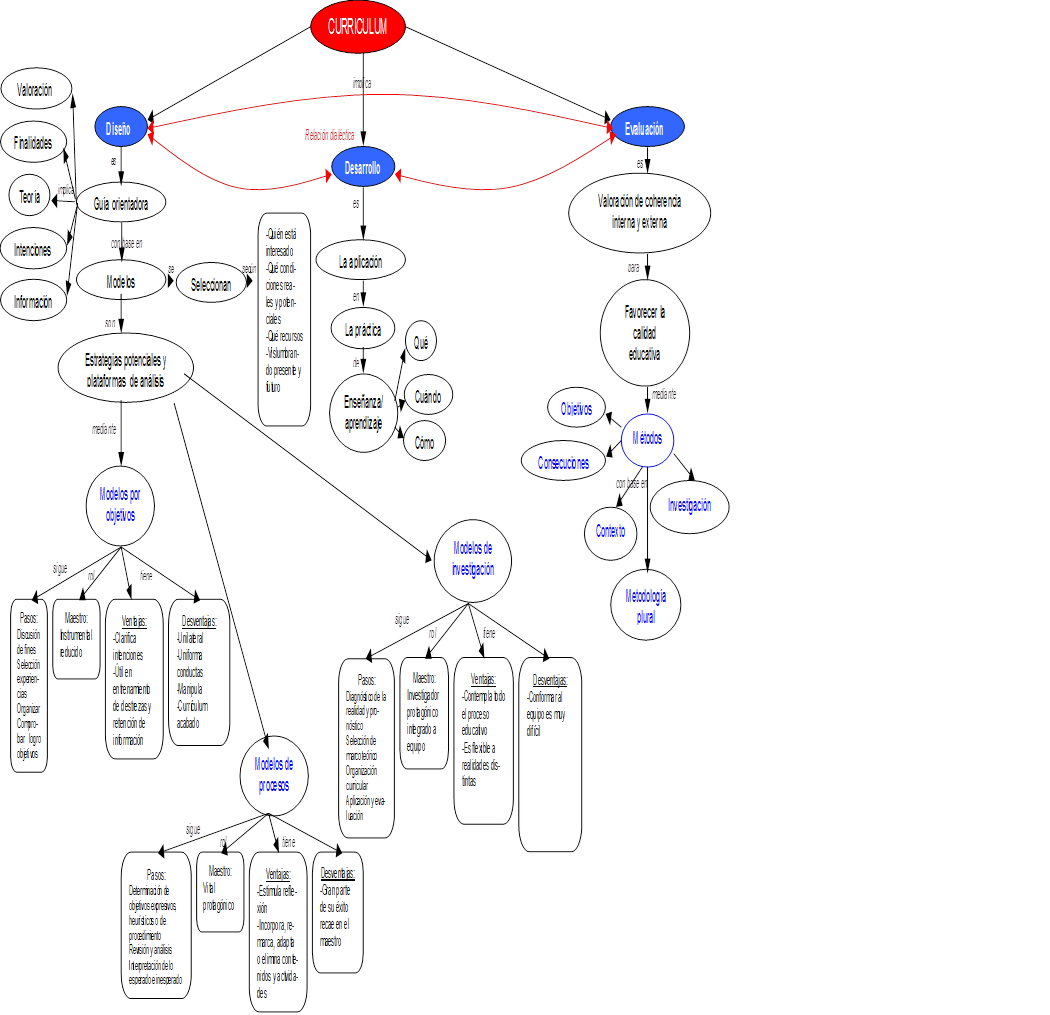
\includegraphics[width=16cm,height=16cm]{p3-img001.png}}
\end{figure}

{\footnotesize {\bfseries Fuente:} elaboración propia con base en Casarini (1999) y 
Stenhouse (1998).}
\newpage

Como referentes me basé en el modelo educativo orientado a la persona y  el cognitivo, así como en el enfoque constructivista, ya que lo consideré 
adecuado debido a la diversidad social, cultural y de procedencia de nuestro 
alumnado. Asimismo, sopesé las ventajas y desventajas de cada modelo 
para, acorde con la realidad y las intenciones pedagógicas, focalizar 
los aspectos positivos. 

En cuanto al sustento teórico, revisé tanto teorías sobre diseño 
curricular como sobre pedagogía, con la intención de que las y los 
alumnos que cursen esta Línea Terminal cuenten con conocimientos y 
herramientas que les permitan darle un giro mucho más dinámico, reflexivo 
y motivador a la enseñanza de la historia, sin descuidar el 
cumplimiento de los contenidos que estipulan los programas educativos 
del nivel en el que probablemente se desempeñen. 

Cabe señalar que el diseño inicial de la Línea Terminal fue discutido por la 
Comisión de reestructuración, integrada por cinco colegas. En este diseño curricular 
pusimos especial énfasis en la importancia de clasificar los objetivos tanto del Plan como 
del Programa de estudios. 

\enlargethispage{-1\baselineskip}
Como resultado del proceso, el actual Plan de estudios de  la 
Licenciatura en Historia de la UAQ, que se comenzó a implementar en 
agosto del 2010, tiene tres líneas terminales: Investigación, 
Patrimonio Histórico Cultural y Enseñanza de la Historia. La demanda 
para cada línea la conocemos al final del quinto semestre, que cuando el 
que el alumno decide. Cabe señalar que se ha documentado que el 
currículum oculto de las licenciaturas de Historia, en general, 
privilegia la investigación histórica sobre otras tareas propias del 
historiador (Rivera~2012). Díaz Barriga (2003,~p.~7) señala que el 
concepto de currículo oculto de \mbox{Jackson~(1968)}:
\newpage

\begin{quotation}
Restablecía la perspectiva que hemos denominado de 
la experiencia, articulando una serie de aprendizajes no explícitos en 
un plan de estudio, que no son intencionados, pero que se muestran 
altamente eficaces. Estos aprendizajes son resultado de la interacción 
escolar y en el aula; en este sentido, son resultados de la 
experiencia. 
\end{quotation}

Para Casarini (1999,~p.~42), <<El currículo se convierte en el mediador 
entre la escuela y la sociedad para lograr transmitir las intenciones 
educativas de una sociedad en determinado momento>>. 

Nuestro actual Programa de estudios busca que las y los alumnos 
desarrollen un papel activo y de responsabilidad frente al proceso 
educativo, por lo que toma como referente el enfoque constructivista, el 
cual propone que el conocimiento es parte integral de la actividad en la 
que se le adquiere,  y es significativo cuando ocurre en contextos 
relevantes y auténticos. Para esto, una de las características 
esenciales del diseño general de la licenciatura que nos ocupa es que 
el alumnado pueda cursar una materia genérica de cada una de las líneas 
terminales, ya sea en cuarto o quinto semestre, a fin de que su 
elección pueda tener elementos sustentados. La materia genérica o 
panorámica (obligatoria para quinto semestre) de la Línea Terminal que 
estamos abordando se denomina Enseñanza de la Historia, en ésta las y 
los alumnos adquieren los elementos necesarios para problematizar la 
práctica de la enseñanza de la Historia en diferentes ámbitos y 
contextos, cuestionar prácticas tradicionales de este quehacer a partir 
del análisis de modelos educativos, así como la revisión de su propia 
vida académica. Así, las y los estudiantes construyen elementos de 
decisión para ponderar si la Línea Terminal en Enseñanza de la Historia 
es su opción de especialidad (Latapí~2012).  
\newpage

%\enlargethispage{1\baselineskip}
El objetivo de la Línea Terminal en Enseñanza de la Historia 
enuncia que

\begin{quotation}
El egresado de la Licenciatura en Historia que haya cursado la Línea 
Terminal en Enseñanza de la Historia, tendrá las herramientas teóricas 
y metodológicas necesarias para participar en diversos ámbitos 
educativos: trabajo frente a grupo, servicios educativos en museos y 
elaboración de materiales educativos, entre otros. Podrá realizar su 
labor profesional con fundamento en el conocimiento del contexto en el 
que incidirá (UAQ 2010, p. 36).
\end{quotation}

Del sexto al octavo semestre, el alumnado de la Línea Terminal en 
Enseñanza de la Historia cursa seminarios, talleres y tópicos selectos 
especializados. <<Para la gradación, secuencia y tipo de asignaturas a 
ofrecer consideramos sustancial que el planteamiento de vinculación 
disciplinar estuviera al día en los paradigmas de la epistemología de 
las ciencias sociales, las psicopedagogías y la disciplina de la 
Historia>> (Latapí~2012,~p.~108). De esta manera, tuve presentes los niveles de 
Jantsch, retomados por Torres Santomé~(2000), y definidos sintéticamente 
de la siguiente manera: multidisciplinariedad como coordinación en el 
nivel más bajo, pero con comunicación incipiente; pluridisciplinariedad 
como intercambio de informaciones en un nivel de igualdad  jerárquica, 
con la virtud de que se unifican conocimientos de diferentes 
disciplinas, pero bajo la consigna de que se mantenga lo específico de 
cada una; disciplinariedad cruzada en la que una de las disciplinas 
domina sobre las otras, interdisciplinariedad que rebasa el reunir 
disciplinas en una marco u objetivo amplio, pues implica 
intercomunicación, trasformación  conceptual y metodológica con un 
equilibrio de fuerzas encaminadas a detectar y solucionar problemas de 
manera compleja; y transdisciplinariedad como la integración de alto 
nivel que posibilita la aparición de una metadisciplina.
\newpage

En lo que respecta al diseño de la  Línea Terminal en Enseñanza de la 
Historia en la UAQ, me enfoqué a rebasar los tres primeros niveles y a 
situar el Plan y Programa en el cuarto. La base sobre la cual 
construirlos parte de la idea de que de primero a quinto semestre los 
alumnos cursaron las asignaturas del eje formativo básico por medio del 
cual adquieren los conocimientos fundamentales de Historia, 
considerando los procesos históricos de larga duración de Europa, 
América, Asía y África, México y, finalmente, Querétaro y su región, 
desde una perspectiva que pretende no ser eurocéntrica. En cuanto al 
tiempo, se abarca desde los grupos prehispánicos, tanto de Mesoamérica y 
la región Andina, como de las primeras culturas clásicas, hasta el 
siglo XX\@. Se inicia en primer semestre con una materia que remite al 
mundo actual, de modo  que los alumnos establezcan relaciones del pasado con 
el presente.  También ya cursaron el eje formativo disciplinar, cuyo 
objetivo es dotarlos de herramientas teóricas y metodológicas 
necesarias para aprender el oficio de historiar, en las que llevan 
asignaturas relativas a las historiografías, a la escritura de la 
historia, a la teoría de la historia,  la historia oral y la 
paleografía, entre otras.  

\enlargethispage{1\baselineskip}
El diseño de los contenidos mínimos de los seminarios, talleres y 
asignaturas buscó la interrelación en el nivel de 
interdisciplinariedad. Espitia~(2002,~p.~16), señala que <<Entendemos la 
interdisciplinariedad como sinónimo de unión de las diferentes áreas en 
las que, de manera tradicional, se ha dividido el conocimiento>>.  
Asimismo, este autor agrega que
\begin{quotation}
La academia había hecho una división arbitraria, aunque no por ello 
ilógica de los contenidos de las materias. Dicha división responde más 
a las necesidades de transmisión que a la lógica del desarrollo de las 
disciplinas. Por esta razón, se hizo necesario pensar incluso los 
contenidos desde otra perspectiva. \ Al mismo tiempo los epistemólogos 
ponían \ en cuestión la excesiva especialización de la ciencia en la 
\mbox{actualidad}. Ambas cuestiones, la de la educación y la de la 
epistemología, aterrizan en el mismo lugar: \ la búsqueda de una 
concepción interdisciplinaria \ de los fenómenos. La 
interdisciplinariedad es solidaria con el pasaje de un pensamiento 
eminentemente racionalista a otro más complejo (\textit{ibid.}, p. 27).
\end{quotation}
%\newpage


Partiendo de la necesidad  que subyace en lo reseñado arriba, hoy entendemos 
que  la educación del siglo XXI debe tomar en cuenta
la cuestión de la interdisciplina como un aspecto medular, de tal forma que pueda encarar, explicar e intervenir en la complejidad de
la realidad social, y que deba plasmarse en todo el programa educativo (Latapí~2013). Por ello, antes de su implementación consideré que deberíamos estar conscientes de algunos puntos que se señalan enseguida: 

\enlargethispage{1\baselineskip}
Sabemos de sobra que en la <<aplicación>>  del Plan  y  Programa ---y que \ más \
que  ello será  una \ <<construcción>> \ en el vínculo entre docentes y alumnos--- un 
factor fundamental es el mediador que pueda enlazar y hacer 
significativos los saberes.  Así, pues, para nosotros, tanto al realizar 
el diseño curricular de la licenciatura y de las líneas terminales, 
como en la selección del personal docente para su implementación, hemos 
contemplado esta visión interdisciplinar, incluyendo a profesoras y 
profesores provenientes de diversas áreas de las ciencias sociales 
(psicología, antropología, educación,  comunicación, especialistas 
en equidad e igualdad de género, entre otros), buscando con ello llevar 
al alumnado a situarse en el lugar de protagonista del análisis e 
investigación del pasado, de sus herencias y memorias legadas a través 
del patrimonio, y de su enseñanza, de tal forma que pueda generarse en 
las futuras generaciones de estudiantes, ese gusto y comprensión por el 
estudio y el aprendizaje de la Historia, utilizándola como una asignatura 
que le permita la reflexión y el análisis del pasado, de una forma ágil y 
constructiva, de tal suerte que consiga aprender de ese pasado, y pueda 
mejorar el presente y el futuro de la sociedad a la que pertenece y el de 
su país. Así, entonces, con las 
diversas miradas sobre la realidad con que este profesorado media en nuestros 
estudiantes  y la complejidad de la interacción de la historia con 
otras ciencias sociales, también se presenta un balance cuando se integra con 
las miradas de los docentes que son historiadores (Latapí~2013). 

\enlargethispage{1\baselineskip}
Los contenidos mínimos de las asignaturas de  la  Línea Terminal en Enseñanza de la Historia, están engarzados entre sí. Enseguida doy cuenta de éstos. 
\begin{Obs} 
\item[$\star$] En sexto semestre los alumnos cursan dos 
seminarios, un taller y una asignatura de tópicos selectos. En el 
\textit{Seminario de Problemas de la Historia: perspectiva 
psicopedagógica\/} los alumnos,  con base inicial en lo abordado en 
otras asignaturas sobre todo del eje formativo disciplinario (La 
disciplina de la Historia y Enseñanza de la Historia de manera directa), 
deben identificar y conocer los principales problemas vinculados con la 
enseñanza de la Historia y que son derivados del carácter propio de los 
constructos de la disciplina, y analizarlos a la luz de los aportes de 
la psicología del desarrollo. También deben investigar un problema específico 
elegido a partir de sus intereses, y lo relacionarlo con un nivel 
educativo, para de ahí plantear posibles soluciones pedagógicas. La 
definición inicial de los problemas parte de los estudios realizados por 
Andrea Sánchez Quintanar, entre los que se encuentran los relativos 
al tiempo y espacio históricos, la causalidad, los sujetos de la historia. En el 
\textit{Seminario Ámbitos en la enseñanza de la Historia/} los alumnos 
analizan los diferentes ámbitos en los que se desarrolla la enseñanza 
de la historia: familia, escuela, medios de comunicación, Internet, 
barrios, museos, iglesias, ámbitos laborales y <<no lugares>>. 
Obedeciendo a sus intereses, elegirán un ámbito, e investigarán sus 
características económicas, sociales, políticas, culturales e 
ideológicas, a fin de identificar implicaciones concretas para la enseñanza 
de la historia. Los alumnos relacionarán dichos resultados de la
investigación con el problema vinculado a la enseñanza de la historia 
que trabajen en el {\itshape Seminario de Enseñanza de la Historia 1\/}, de tal
suerte que las soluciones pedagógicas planteadas sean adecuadas al contexto.  
En el \textit{Taller de Recursos Didácticos 1\/} los alumnos analizan 
críticamente diversos recursos educativos para la enseñanza de la 
historia (contenidos en programas, libros de texto, de divulgación y 
páginas web, entre otros) y diseñan uno de manera sustentada. La 
asignatura de \textit{tópicos selectos\/} es una materia cuyo contenido 
se establece de acuerdo con los intereses concretos de los alumnos.
\item[$\star$] En séptimo semestre las y los estudiantes cursan el 
\textit{Seminario de Praxis Docente\/}, en el que, con base inicial en lo 
abordado en los Seminarios de investigación 1 y 2, desarrollan un 
trabajo en el que deben articular la pertinencia teórica, el contexto y 
el ámbito elegido a la praxis docente. Los alumnos deben conocer  y 
tomar postura frente a los factores que inciden en una buena praxis 
docente. Aquí interviene la mediación de un proceso personal que no se 
ha mencionado y que es la propia experiencia de vida con respecto a 
docentes que han formado a los propios alumnos para hacer un ejercicio 
de toma consciencia, por ser este un factor que incidirá de manera 
directa en la praxis del alumno cuando sea docente. En el 
\textit{Seminario de Integración de problemas, ámbitos y praxis 
docente\/}, los  alumnos,  con base inicial en lo abordado en los 
Seminarios de Investigación 1 y 2, desarrollan un trabajo en el que 
articulan la pertinencia teórica, el contexto y el ámbito elegido que 
sustente su trabajo de titulación. En el {\itshape Taller de Recursos 
Didácticos II\/} \ los alumnos, apoyándose en el diseño del recurso 
didáctico que realizaron al principio en el {\itshape Taller de Recursos 
Didácticos~1\/}, desarrollan dicho recurso (con pertinencia pedagógica y 
disciplinar), lo finalizarán, lo aplicarán y lo evaluarán. Para ello podrán
valerse de las herramientas obtenidas en otras asignaturas, 
principalmente la de {\itshape Tecnología aplicada a la divulgación de la historia 1\/} y 
{\itshape 2}\@. 
\end{Obs}

\enlargethispage{1\baselineskip}
Siguiendo con la manera en que se ha buscado implementar una mirada 
interdisciplinaria, en la Licenciatura en Historia hemos fomentado que 
los estudiantes de la Línea Terminal en Enseñanza de la Historia, 
comprendan la necesidad de usar las fuentes del conocimiento histórico 
(investigación histórica) y del patrimonio cultural, tanto para 
sustentar argumentos como para ofrecer a los alumnos con quienes 
interactúan en sus prácticas profesionales, herramientas que les 
permitan problematizar la realidad histórica a través de procesos de 
enseñanza-aprendizaje, que les lleven a unir las asignaturas que cursan 
---que a sus ojos aparecen fragmentadas--- (historia, formación cívica, 
ética, geografía). En dichas asignaturas emergen algunas temáticas, como el 
cuidado del medio ambiente, la preservación, protección y conservación 
del patrimonio histórico cultural (en sus diferentes vertientes), los 
derechos humanos, entre otras, que sólo pueden ser abordadas desde la 
interdisciplina si se quiere lograr que dichos alumnos (adolescentes, 
principalmente) comprendan que las asignaturas son, precisamente, 
miradas sobre la realidad social que si las ponemos en tensión 
cognitiva y emocional, nos permiten asirla para comprenderla.

%\enlargethispage{1\baselineskip}
Así también, en la Línea Terminal en Enseñanza de la Historia, 
consideramos que las didácticas de la historia son de suma importancia para que 
los futuros docentes orienten a sus alumnos hacia aquellas tareas que 
generen niveles de comprensión altos y creativos, a través de plantear 
problemas y generar dinámicas que conduzcan al estudiantado a realizar 
preguntas al objeto o fenómeno, en búsqueda de la información histórica 
necesaria, y  hacia la reflexión teórica, partiendo de la relación que 
tenga la información recabada con los conocimientos, así como de la comunicación que 
sostenga con sus compañeros, sus profesores, especialistas en la materia y otros 
sujetos implicados en el proceso (Ferreiro,~López,~López, y~López~ 2004). 
El segundo referente que consideramos que deben tener nuestros 
estudiantes de las tres líneas terminales, es la búsqueda de la 
explicación histórica mediante la multidisciplinariedad, cuestión que 
reforzamos con los perfiles de nuestros docentes, quienes, como ya se 
mencionó, proceden de diversos campos de las ciencias sociales, con 
experiencias profesionales diversas. 

En cuanto a la aplicación de la perspectiva interdisciplinar en la 
Línea Terminal de Patrimonio, consideramos que éste, al ser 
un testimonio de toda una época, sirva, a través de objetos y 
manifestaciones relacionadas con la vida política, económica, social y 
espiritual de un lugar en un momento dado, como medio de 
enseñanza, y le permite al estudiante tener una visión más integral del 
contenido del aprendizaje. 

En cuanto a los alumnos que cursan la Línea Terminal en Investigación 
Histórica, se les fomenta la comprensión de la relación e incidencia 
que su trabajo tendrá a la hora de enriquecer el de sus compañeros que 
cursan las otras líneas terminales, así como lo fundamental que 
resulta nutrir su propio aprendizaje y el futuro desempeño profesional  
mediante la utilización de herramientas y conocimientos propios de 
disciplinas diversas, sin dejar de lado que, muy posiblemente, en su 
vida laboral enfrentarán situaciones que tendrán que ver con el 
patrimonio y la enseñanza en sus diversos ámbitos (enseñar siendo 
profesores universitarios, enseñar en un museo, enseñar en una 
publicación de cualquier índole, \ldots). 

%\enlargethispage{1\baselineskip}
Bajo tal supuesto se instrumentó  la materia de {\itshape Museos\/}, en la cual los alumnos deben desarrollar investigaciones y valerse de lo
aprendido sobre patrimonio para lograr generar, dentro de los museos, un espacio para enseñar historia.  Como
coordinadora de la Línea Terminal en Enseñanza de la Historia, he participado como invitada  en dicha asignatura,
experiencia que constituye un proceso colaborativo y que abre espacios para patentizar un currículum flexible.
%\newpage 

\medskip
\textbf{Resultados}

En el proceso de ponderar los diversos aspectos en vías a realizar modificaciones al Plan y Programa de estudios en el
2015, hemos diseñado y aplicado cuestionarios de evaluación a docentes y estudiantes, que ponen atención en la planeación de clases, la autorreflexión, el proceso de enseñanza-aprendizaje, la percepción global y particular de la Línea Terminal en Enseñanza de la Historia, así como en las prácticas profesionales y de servicio social. El análisis de estos cuestionarios nos arroja lo siguiente:
%\newpage

\bigskip
\begin{center}
\begin{tiny}       % otherwise, table won't fit
%\begin{table*}[h]
\tabulinesep=1.5mm
\begin{longtabu*} to \textwidth {X[5,l,p]|X[5,l,p]}
    %{X[50,l,l] | X[50,l,l]}
    %\caption[{}]\label{tab:label}\\ %
    \toprule
    %\hline \hline
\rowcolor{lsLightBlue}\textbf{DOCENTES} & \textbf{ALUMNADO}\\ 
    \midrule
  \endfirsthead%
%\hline \hline \hline \hline
%\begin{flushleft}
%\begin{table}[H]
%\begin{center}
%\begin{tiny}  % otherwise, table won't fit
%\tablefirsthead{%
%\hline
%{\bf DOCENTES} & {\bf ALUMNADO}\\
%\hline}
%\tablehead{}
%\tabletail{}
%\tablelasttail{}
%\bottomcaption{Figura 1. }
%\tablehead{\hline
%{\bf DOCENTES}  &
%\arraybslash{\bf ALUMNADO} \\\hline}
%\begin{supertabular}{|p{0.5\linewidth}|p{0.5\linewidth}|}
%\hline
%{\bf DOCENTES} & {\bf ALUMNADO}\\ 
%\hline
%\begin{center}
%\begin{landscape}
%\small  % otherwise, table won't fit
%\setlength\LTleft{-30pt}            % default: \fill
%\setlength\LTright{-30pt}           % default: \fill
%\begin{longtable}{|p{80mm}|p{80mm}|}
%\hline\hline 
%\multicolumn{1}{|l|}
%\footnotesize  % otherwise, table won't fit
%\setlength\LTleft{-30pt}            % default: \fill
%\setlength\LTright{-30pt}           % default: \fill
%\begin{longtable}{@{\extracolsep{\fill}}ll@{}}
%\hline\hline %inserts double horizontal lines
%{\bf DOCENTES} & 
%\multicolumn{1}{l|}
%{\bf ALUMNADO} \\ [0.5ex] \hline
%\endfirsthead 
%\multicolumn{2}{l}%
%{{\bfseries \tablename\ \thetable{} -- continuación}} \\
%Continuación de la tabla \\
%\hline 
%\multicolumn{1}{|l|}{
%{\bf DOCENTES} &
%\multicolumn{1}{l|}{
%{\bf ALUMNADO} \\ [0.5ex]  \hline 
%\endhead
%\hline \multicolumn{2}{|r|}{{continuación}} \\ \hline
%\multicolumn{2}{|r|}{{Continúa en la siguiente página}} \\
%\hline
%{ } & continúa... \\\hline \begin{tiny}
%\endfoot
%\hline
%{\bf DOCENTES} & 
%\multicolumn{1}{l|}{
%{\bf ALUMNADO} 
%\hline \hline
%\endlastfoot
%\endlastfoot
%\caption[(Cont)]
\multicolumn{2}{r}{{Viene de la página anterior\ldots}} \\ \midrule %\hline
%{\emph{Continuación}}\\%
\toprule
\rowcolor{lsLightBlue}\textbf{DOCENTES} & \textbf{ALUMNADO}\\ 
\midrule
\endhead%
\bottomrule
\multicolumn{2}{r}{{Continúa en la siguiente página\ldots}} %\\\ %hline
\endfoot%
%
%\hline
\midrule\endlastfoot%
% Now the regular content:
\rowcolor{lsLightGray} \textbf{Autorreflexión} 

Interés docente por compartir conocimientos y experiencia profesional 
en diferentes ámbitos con las y los alumnos, con la intención de 
incidir positivamente en la mejora en la enseñanza de la historia por 
considerarla vital para educar a los seres humanos en la comprensión, 
la empatía y el humanismo, desarrollando en ellos una visión que les 
permita conocer sus orígenes, quienes son y cómo pueden enriquecer su 
presente. 

La mayoría de las y los docentes hicieron recomendaciones al alumnado
para mejorar la redacción y ortografía, exposición en clase, aprendizaje, 
presentación de trabajos y actitud en clase. 
&

{\bfseries Autorreflexión}

Interés del alumnado por aportar a las futuras generaciones una visión
diferente de la historia, su aprendizaje y su enseñanza.

Las y los alumnos consideran que escucharon y pusieron en práctica
todas las sugerencias de mejora y recomendaciones que les hicieron las y los 
docentes.\\
%\midrule
\addlinespace
\rowcolor{lsLightGray} {\bf Planeación de clases}

Las y los docentes entregan un programa del curso y lo comentan con el
alumnado, aclarando dudas, técnicas de enseñanza, fuentes de información y formas 
de evaluación. 

La mayoría piensa que la secuencia, orden y relación de presentación y
trabajo de los temas que se ven en clase permiten al alumnado lograr un aprendizaje significativo. 

Algunos docentes consideraron que un área de mejora es la comunicación
entre docentes para conocer los contenidos de sus asignaturas, áreas de oportunidad del alumnado y 
cargas de trabajo asignadas a las y los alumnos. 
&
{\bfseries Planeación de clases}

Las y los alumnos coinciden con la respuesta de las y los docentes en
cuanto a la entrega y discusión del programa del curso.  

La respuesta del alumnado coincide con la de las y los docentes.\\
%\hline
\addlinespace 
 
\rowcolor{lsLightGray} {\bfseries Proceso enseñanza–aprendizaje}

La mayoría de las y los docentes:

\begin{itemize}
\item Utilizan como materiales la Antología que entregan al inicio del
curso, libros, diagramas, esquemas y mapas conceptuales. 
\item  Relacionan la teoría con ejemplos y\slash\o situaciones
prácticas.
\item  Las principales fuentes y medios que promueven para la consulta
de información son: la biblioteca, Internet, revistas y libros. 
\item Brindaron asesoría al alumnado.
\item Consideraron que el ambiente de trabajo en clase fue bueno o
regular.
\item  Consideran que las asignaturas de la Línea Terminal, así como las
de ésta con las de las de otras de la licenciatura y Líneas Terminales, se relacionan mucho entre sí. 
\item Coinciden en evaluar la actitud para el aprendizaje de las y los
alumnos entre buena y regular. 
\item  Utilizan como forma de evaluación los exámenes y trabajos
escritos, trabajo e investigación de campo, exposición en clase y tareas. 
\item  Durante el desarrollo del curso fomentan la discusión en clase,
la crítica razonada, el auto aprendizaje, el razonamiento científico, el trabajo en equipo De los 7 docentes solamente
3 fomentaron la utilización de la perspectiva de género en el desarrollo del curso (2 de ellas ya no colaboran con
nosotros).
\item  Encontraron que las y los alumnos solamente a veces y en algunos
casos, revisan y ponen en práctica las sugerencias de mejora o correcciones hechas a sus trabajos.
\end{itemize}
&
{\bf Proceso enseñanza-aprendizaje}

La mayoría de las y los alumnos: 

\begin{itemize}
\item  Utilizan y les son de mayor utilidad los materiales como:
antología, libros de texto, vídeo, ejercicios prácticos, diagramas, esquemas y mapas conceptuales. 
\item Coinciden en que las asignaturas que relaciona más la teoría con
la práctica son Taller de Recursos Didácticos I y II\@. 
\item Consideran que la dinámica principal de las clases son
expositivas, con participación de ellas y ellos. 
\item  Opinan que las principales fuentes y medios que las y los
docentes promovieron para la consulta de información fueron: Antologías de textos, páginas de Internet y libros.
\item Dijeron que las y los docentes les brindaron apoyo o asesoría
cuando se les solicitó. Opinaron que el nivel de calidad y apoyo brindado fue bueno (en un rango de excelente a malo).
\item  Consideraron que el ambiente de trabajo promovido por las y los
docentes fue bueno (en un rango de excelente a malo).
\item  Consideraron en promedio como <<bueno>> el nivel de conocimiento de
la asignatura por parte de las y los docentes (en un rango de excelente a malo). En este punto hubo contradicciones
pues hay calificaciones de excelente, malo y regular para un mismo docente. 
\item  Opinan que las asignaturas de la LT se relacionan <<más o menos>>
con otras de la licenciatura o de las otras LT\@. 
\item  Consideran que en las formas o criterios de evaluación predomina
el trabajo escrito, el proyecto y las tareas. 
\item  Consideran que dos docentes promueven la discusión en clase, la
crítica razonada, el autoaprendizaje, la perspectiva de género, el razonamiento científico, el trabajo en equipo. Tres
docentes promueven los trabajos de investigación y el análisis de la relación de lo sucedido a nivel internacional en
una misma época con el presente.
\item  Consideran que la mayoría de las y los docentes dieron
retroalimentación a sus trabajos y tareas. 
\item Consideran que los contenidos de la LT son actuales, relevantes
para su formación y comprensibles. 
\end{itemize}

Las respuestas en cuanto a las y los profesores que impulsan o no la
participación en clase para mejorar el aprendizaje fueron variadas y 
contradictorias.\\
%\hline
\addlinespace
 
\rowcolor{lsLightGray} {\bfseries Percepción global}

La mayoría de las y los docentes:

\begin{itemize}
\item  Evaluaron bajo la actuación conforme a valores de parte del
alumnado, así como la actitud hacia el aprendizaje y el compañerismo. 
\end{itemize}
&
{\bf Percepción global}

La mayoría de las y los alumnos:

\begin{itemize}
\item  Evaluaron alto a las y los docentes en cuanto a la promoción de
valores en su praxis docente. 
\end{itemize} \\
%\midrule
\addlinespace 

\rowcolor{lsLightGray} {\bfseries Percepción Línea Terminal}

La mayoría de las y los docentes consideraron que:

\begin{itemize}
\item  Los mejores aspectos de la Línea Terminal son la relación de los temas
entre las asignaturas, el programa de estudios, las prácticas profesionales, los eventos (congresos, seminarios, etc.) que fortalecen el aprendizaje y el servicio social. 

\item Las fortalezas de la Línea Terminal (LT) son: el entusiasmo de las y
los docentes; el eje formativo permite al alumnado aplicar y relacionar los conocimientos previos; impulsa una
formación integral que afianza a las materias con las actividades fuera del aula; formar historiadores como enseñantes,
con estrategias didácticas y fundamentos pedagógicos.

\item Las debilidades de la Línea Terminal son: al inicio del semestre 
el alumnado se enfrenta con temas y dinámicas nuevas; las y los alumnos 
se sienten menos que los que cursan otras LT\@; relacionar los contenidos 
de las asignaturas y especialmente los trabajos y proyectos de forma 
horizontal, promover la colaboración y comunicación entre el 
profesorado; fortalecer la exposición en clase por parte del alumnado, 
así como la utilización de la perspectiva de género, tanto en la praxis 
docente como en la investigación y enseñanza de la historia.

\item  Las áreas de oportunidad de la Línea Terminal son: fortalecer el
trabajo colectivo docente así como las habilidades de investigación, aun cuando la especialidad sea en enseñanza; mejorar el compromiso de las y los alumnos.

\item El alumnado debe fortalecer la capacidad de análisis y abstracción,
síntesis, redacción, metodología de investigación, utilización de las TIC, idioma inglés.

\item Considera que las asignaturas de la LT son de utilizad para el
desempeño del alumnado en diferentes ámbitos en la enseñanza de la historia. 
\end{itemize}
&
{\bf Percepción Línea Terminal}

La mayoría de las y los alumnos consideraron que: 

\begin{itemize}
\item Los aspectos que más les han gustado de la LT son: las prácticas
profesionales, el servicio social y los eventos. 
\item Las asignaturas cursadas en la LT les son de utilidad para
desempeñarse en diferentes ámbitos en la enseñanza de la historia.
\item  La cantidad de lecturas y trabajos por semestre fueron apropiados
para su aprovechamiento académico. 
\end{itemize} \\
%\midrule
\addlinespace 
 
\rowcolor{lsLightGray} {\bf Servicio social y prácticas profesionales}

Algunos docentes consideran que los lugares en donde las y los alumnos
realizan su servicio social y prácticas profesionales son los adecuados pues pueden practicar la docencia. 
&
{\bf Servicio social y prácticas profesionales}

La mayoría de las y los alumnos considera que:

\begin{itemize}
\item El servicio social contribuye a su consolidación académica.
\item Las prácticas profesionales que realizaron contribuyen a su
formación para la enseñanza de la historia. 
\end{itemize} \\
%\hline
\addlinespace
\bottomrule
\end{longtabu*}

%\end{supertabular}
%\end{longtable}
%\end{table}
%\end{flushleft}
%\caption*{Cuadro 1}
%\end{footnotesize}\end{center}
%\end{table*}
%\end{center}
\end{tiny}\end{center}
\normalsize
\newpage

Actualmente, la primera generación de la Línea Terminal en Enseñanza de la Historia está finalizando sus estudios y, aun cuando a lo largo del camino hubieron encuentros y 
desencuentros entre el alumnado y las y los docentes, la línea está bien valorada, como se puede
colegir de las evaluaciones en cuanto al ambiente de trabajo, así como en las del 
profesorado en cuanto a actuación conforme a valores, actitudes frente al aprendizaje, compañerismo y puesta en práctica de la retroalimentación. Con
base en ello podemos decir que, a mitad de camino, tenemos tanto resultados positivos 
y prácticas para volver a implementar,  como áreas de posible mejora. 

Desde el punto de vista tanto de las y los docentes como del alumnado, las siguientes son las fortalezas de esta línea terminal: considerar que las asignaturas cursadas 
en ella son de utilidad para que el alumnado se desempeñe 
en diferentes ámbitos en la enseñanza de la historia; el gusto y la
pertinencia de la realización y la asistencia a eventos; la repercusión de las 
prácticas profesionales y el servicio social, pues le permite al alumnado poner en 
práctica las estrategias y teorías aprendidas en la especialidad. Un 
aspecto  que demanda especial atención es la diferencia en la percepción entre 
alumnado y el profesorado sobre la relación que se da entre las asignaturas cursadas 
en la Línea Terminal en Enseñanza de la Historia con otras de la licenciatura 
o de otras Líneas Terminales. 

\enlargethispage{1\baselineskip}
Como debilidades encontramos la necesidad de fortalecer la investigación y la exposición en clase por parte del alumnado,
así como el fomento de la discusión en clase y la crítica razonada, así como la utilización de la perspectiva de
género, tanto en la praxis docente como en la investigación y enseñanza de la historia. Asimismo, es importante crear
una biblioteca con materiales específicos para las y los estudiantes de nuestra Línea Terminal.

Las áreas de oportunidad que detectamos se refieren, básicamente, a la necesidad de fortalecer el trabajo en colectivo de las y los docentes, así la capacidad de análisis y abstracción, síntesis, redacción, metodología de la investigación, utilización de las TIC y de materiales en inglés por parte de las y los alumnos. 

\bigskip
\noindent {\bfseries Referencias}
\enlargethispage{1\baselineskip}

\medskip
Casarini, M\@. (1999), \textit{Teoría y diseño curricular}, México, Ed\@. Trillas-UV\@. 

Díaz Barriga, A. (2003), <<Currículum. Tensiones conceptuales y prácticas>>. En 
\textit{Revista Electrónica de Investigación Educativa, 5}. Consultado el 3 de marzo de 2011 en \\
\url{http://redie.uabc.mx/vol5no2/contenido-diazbarriga.html}

\begin{sloppypar}
Ferreiro, R., López, J., López, L. y López, J. (2004), <<El patrimonio cultural entre los medios de enseñanza de la Historia>>. \textit{Ilustrados, 1--4}. Recuperado el 12 de marzo del 2013 de \url{http://www.ilustrados.com/tema/7180/patrimonio-cultural-entre-medios-ensenanza-Historia.html}
\end{sloppypar}

Latapí, P. (2012), \textit{Construyendo sobre las miradas en torno a la enseñanza de 
la Historia}. En Latapí, P., Miró, M. y Somohano, L. (coords), \textit{Miradas diversas. Estudios Antropológicos, Históricos y Filosóficos},\\ pp.106--116. México, UAQ-Facultad de Filosofía.  

Latapí, P. (2013), La interdisciplinariedad en las Licenciaturas en Historia. En \textit{VIII Encuentro de la Red Nacional de Licenciaturas en Historia y  Cuerpos Académicos y $2^\circ$  Encuentro Iberoamericano de Licenciaturas}. En \textit{Historia. <<Currículo, formación y práctica docente en la enseñanza de la Historia>>}, Morelia, Michoacán, Facultad de Historia, Universidad Michoacana de San Nicolás de Hidalgo.

Luhmann, N. (1973), \textit{Ilustración sociológica y otros ensayos}, Buenos Aires, Sur.

Rivera Gómez, E. (2012), <<Investigación y enseñanza de la Historia: una reflexión desde la práctica académica>>. En Latapí, P., Miró, M. y Somohano, L. (coords). \textit{Miradas diversas. Estudios Antropológicos, Históricos y Filosóficos}, (pp. 18--24). México, UAQ-Facultad de Filosofía.  

Stenhouse, L. (1998), \textit{Investigación y desarrollo del currículum}, Madrid, Morata.

Torres Santomé, J. (2000),  \textit{Globalización e interdisciplinariedad: el currículum integrado}, Madrid, Morata.

\begin{sloppypar}
Wallerstein, I\@. (1996), \textit{Abrir las ciencias sociales}, México, Siglo XXI-Centro de Investigaciones Interdisciplinarias en Ciencias y Humanidades UNAM\@.
\end{sloppypar}

Wallerstein, I\@. (1999), \textit{Impensar las ciencias sociales}, México, Siglo XXI-Centro de Investigaciones Interdisciplinarias en Ciencias y Humanidades UNAM\@.

%\clearpage\setcounter{page}{65}
%\markboth{}{}
\thispagestyle{empty}	
\phantomsection{}
\addcontentsline{toc}{chapter}{La enseñanza de la Historia y su pertinencia\\ en los Planes de Estudio\newline $\diamond$
\normalfont\textit{María Gabriela Guerrero Hernández\\ y María del Rocío Rodríguez Román}}	
{\centering{\scshape \large La enseñanza de la Historia y su pertinencia\\ en los Planes de Estudio} \par}
\markboth{formación del historiador}{la enseñanza de la historia}

\bigskip
\begin{center}
{\bfseries  Ma. Gabriela Guerrero Hernández\\
María del Rocío Rodríguez Román}\\
{\itshape{} Facultad de Filosofía y Letras de la UANL\/}
\end{center}


\bigskip
\noindent{\bfseries Resumen}

La docencia y\slash{}o enseñanza de la historia es una de las 
acentuaciones o fases terminales presentes en las distintas 
Licenciaturas de Historia que se ofertan en México, situación que 
merece ser analizada para identificar qué criterios se han considerado 
al respecto para la denominación de las unidades de aprendizaje que 
conforman y, a la vez, amplían la formación de los futuros Licenciados 
en Historia, así como su contenido. Aspectos por demás importantes para 
comprender la relevancia que esta acentuación cobra en los últimos 
años, sobre todo a partir de las demandas del mundo globalizado que 
requiere de un profesionista con conocimientos actualizados y que estén 
acordes con las necesidades del mercado; lo que lleva a considerar que 
el egresado de Historia no sólo debe ser capaz de explicar los procesos 
socio-históricos por los que ha transitado la humanidad a través del 
tiempo, sino que también debe poseer los recursos didácticos  para 
acercar a las generaciones más jóvenes al conocimiento histórico.\\ 
{\bfseries Palabras clave:} Plan de Estudios, enseñanza de la historia, 
procesos formativos, especialización y malla curricular.
%\enlargethispage{\baselineskip}

\medskip
\textenglish{{\bfseries Abstract}}

\textenglish{History Teaching and its Relevance to the Curriculum 
Teaching of history is one of the accentuations or ending phases in all 
the different degrees in history offered in Mexico. This situation 
deserves to be analyzed to identify the criteria considered in the 
denomination of the learning units that are part, and at the same time 
expanded of the formation of future graduates with a bachelor's degree 
in history and its content. These aspects are vital to comprehend the 
relevancy of this accentuation in the last few years, specially because 
of the demand of our globalized world that requires a professional with 
date knowledge lined whit market needs. This reads us to considerate 
that the graduate whit a bachelors degree in History should not only be 
able to explain the process social-historical by which humanity has 
transited over time but should possess the teaching resources to bring 
the younger generations to the historic knowledge.}\\ 
\textenglish{\textbf{Keywords:} Curriculum, Teaching of History, 
Training Processes, Specialization.}

\medskip 
\noindent La enseñanza de la historia es una de las dos áreas  
principales del quehacer del historiador como bien lo ha señalado Plá 
(2011), no obstante, esta área es poco valorada incluso por los mismos 
historiadores, quienes durante su formación han sido receptores de un 
discurso que privilegia la investigación e interpretación de los hechos 
del pasado, en  menoscabo de la formación orientada hacia la enseñanza 
de la historia, situación que poco se ha llevado a la discusión, en 
parte porque la tradición sigue presente en los procesos formativos de 
los estudiantes de la licenciatura en historia, y, por otra parte, 
porque incluso ni los mismos formadores de esta disciplina han 
reflexionado que una de las bondades de la profesión es también el 
difundir el conocimiento histórico a través de su enseñanza, y que para 
ello se requiere ampliar los saberes presentes en el Plan de Estudios 
bajo el cual se prepara a los futuros licenciados en Historia.  

%\enlargethispage{1\baselineskip}
Cabe señalar que esta preocupación es relativamente reciente en el 
ámbito de la universidad, debido a que en esta institución se mantiene 
la tradición en relación a la promoción de la investigación, lo cual es 
positivo, pero siempre y cuando no se descuiden las otras dos funciones 
sustantivas de la universidad, como son la docencia y la difusión de la 
cultura. Como lo  ha expresado Fabre (2005, p. 6), quien encuentra que desde 
la Organización de las Naciones Unidas para la Educación, la Ciencia y 
la Cultura (UNESCO) se insiste en que las universidades del siglo XXI 
son <<Centros de ciencia y fuente de conocimiento que llevan a la 
investigación teórica o aplicada o a la formación de profesores>>, lo 
cual indica que la docencia y\slash{}o enseñanza de la historia debe 
tener un estatus similar al de la investigación.
 
Quizás esta sea una de las orientaciones que recientemente han permeado 
a la universidad pública, la cual ha entrado en una dinámica de cambio, 
producto de las transformaciones en los distintos campos de la 
sociedad (económico, político, social y cultural), que la han llevado a 
replantearse su papel en la formación de los futuros profesionistas y a 
incorporar las tendencias educativas más actuales en sus Planes y 
Programas de Estudio, como es el modelo educativo por competencias y el 
enfoque del aprendizaje centrado en el alumno.  Tendencias que se 
complementan y sugieren un cambio de paradigma educativo en la 
universidad, quien, atenta a estos cambios, se ha dispuesto a incorporar 
de manera gradual las recomendaciones mediante unos procesos de rediseño 
curricular, cuyo impacto se observa ya en la malla curricular con que se 
forman a los estudiantes; por lo menos es lo que se ha encontrado en la 
revisión que se ha llevado a cabo de los 39 Planes de Estudio ofertados 
en las universidades del país. 
\enlargethispage{-1\baselineskip}

El desarrollo de competencias didácticas en los programas educativos de 
Historia a nivel licenciatura debe ser una parte medular, pues es 
sabido que la docencia y  la investigación  son las actividades 
sustantivas de todo historiador: <<El historiador profesional 
universitario[\ldots] combina una dualidad de funciones bien conocida: es y 
debe ser investigador y enseñante al mismo tiempo>> (Moradiellos 
1994, p. 62). 

Pensar que la tarea del historiador consiste sólo en  crear nuevo 
conocimiento, es decir, en buscar los hechos, analizarlos e 
interpretarlos, es limitar demasiado su función. Por eso la enseñanza 
universitaria de la historia debe incluir tanto la parte disciplinar; 
es decir, el cuerpo de conocimientos de la historia,  como la parte 
práctica, o sea la formación sobre cómo se produce dicho conocimiento, 
y además el elemento didáctico, que hace referencia a cómo enseñar la 
historia. Ya que, como señala Andrea Sánchez Quintanar (1995, p. 3), 

\begin{quotation}
(\ldots) la formación como la información del futuro historiador se orienta 
mucho más hacia la investigación que hacia la docencia, pese a que por el 
contrario, el terreno de la práctica profesional es mucho más amplio en 
la enseñanza escolar. 
\end{quotation}

\enlargethispage{1\baselineskip}
Motivo por el cual resulta necesario conocer en qué medida los 
programas educativos de Historia que, a nivel licenciatura, ofrecen las 
diferentes universidades del país, tanto públicas como privadas, 
contemplan el desarrollo de competencias didácticas en sus estudiantes. 
De acuerdo al Catálogo de la Asociación Nacional de Universidades e 
Instituciones de Educación Superior (ANUIES) 2012,  existen en el país 
34 Instituciones de Educación Superior (IES) incorporadas a esta 
asociación, entre las cuales ofrecen 39 programas de Licenciatura en Historia 
o carreras afines (Ver Anexo 1).  Con base en la información proporcionada en 
las páginas electrónicas de las IES, se hizo una revisión de los 
perfiles de egreso, pues ahí es donde se indica el tipo de 
profesionista que se espera formar, con el propósito de identificar la 
idea que subyace en cada una de ellas respecto a lo que implica el 
oficio del historiador,  misma que se ve reflejada en la malla 
curricular que forma a los estudiantes como futuros historiadores.

De los 39 programas educativos no se localizó el perfil de egreso de 
nueve de ellos, y de los treinta restantes solo en siete no se hace 
ninguna alusión a la docencia, sino que son muy genéricos.  Los 23 
restantes sí señalan que se espera que al egresar los estudiantes se 
desarrollen en la investigación, la docencia, la difusión y\slash{}o 
preservación del patrimonio cultural,  como las áreas fundamentales del 
quehacer del historiador. Lo que indica que, al menos en el discurso, se 
considera que la función del historiador va más allá que la de investigar.

\enlargethispage{1\baselineskip}
Ahora bien, revisando las mallas curriculares se pudo observar lo 
siguiente: no hay proporción entre las unidades de aprendizaje (UA) 
relacionadas con la docencia, la investigación y la difusión, pues dos 
terceras partes se avocan a formar a los estudiantes en la 
investigación, un 21.9\,\% a la docencia y solo un 14.6\,\% a la 
difusión (véase el Cuadro 1). 

\begin{small}
\textbf{Cuadro 1. Unidades de aprendizaje relacionadas con las áreas de 
docencia, investigación, difusión o patrimonio en las mallas 
curriculares} 
\end{small}

\begin{flushleft}
%\tablefirsthead{}
%\tablehead{}
%\tabletail{}
\begin{supertabular}{m{1.7cm}m{1.7cm}m{1.7cm}m{1.7cm}m{1.7cm}m{1.7cm}}
\hline
\multicolumn{2}{>{\columncolor{sLightGreen}} m{3.6cm}}{\centering \bfseries DOCENCIA}&
\multicolumn{2}{>{\columncolor{sLightGreen}} m{3.6cm}}{\centering \bfseries INVESTIGACIÓN}&
\multicolumn{2}{>{\columncolor{sLightGreen}} m{3.6cm}}{\centering \bfseries DIFUSIÓN}\\[1pt]
%\hline

\rowcolor{sLightGreen}{\centering{\textbf{\phantom{ab}No.}}}&\centering{\textbf{\%}}&\centering{\textbf{No.}} 
&\centering{\textbf{\%}}&\centering{\textbf{No.}}&
\centering\arraybslash{\textbf{\%}}\\%\hline

\rowcolor{lsLightGray}\centering{\textbf{66}}&\centering{\textbf{21.9}}&\centering{\textbf{191}}&
\centering{\textbf{63.4}}&\centering{\textbf{44}}&\centering\arraybslash{\textbf{14.6}}\\\hline\hline

\multicolumn{6}{>{\columncolor{lsLightGray}} m{11.2cm}}{\textbf{\footnotesize Fuente:} {\footnotesize Mallas curriculares de las Licenciaturas de Historia incorporadas a la ANUIES.}}\\%\hline
\end{supertabular}
\end{flushleft}
%\newpage

Cabe aclarar que solo se consideraron las 
unidades de aprendizaje que aparecían como obligatorias en las mallas 
curriculares, pues cada programa educativo ofrece varias asignaturas 
optativas relacionadas con estas tres áreas terminales o acentuaciones. 

Respecto al número de UA, destaca el hecho que en seis de los 
39 programas revisados, no se ofrece ninguna materia obligatoria 
relacionada con la formación docente, y que en solo dos de estos programas 
se ofrecen unidades de este tipo,  pero como optativas, lo que significa que no es 
seguro que los estudiantes las elijan. Ahora bien, encontramos que en dos 
de estos programas sí se considera la docencia como parte de la 
formación de los futuros historiadores, aunque no se explica cómo 
lograran las competencias docentes si no cuentan con ninguna unidad de 
aprendizaje relacionada con ello; mientras que en otros tres programas 
están entre los que no se consiguió su perfil de egreso.

\enlargethispage{\baselineskip}
Llama la atención, en este sentido, el caso de la UANL, pues en su plan de estudios 
2005 todas las materias vinculadas con la docencia son de carácter optativo, lo que 
significa que si los jóvenes no eligen esa acentuación salen de su 
carrera sin ninguna base para hacer frente a la actividad docente. Como lo 
constatan las cifras: en las diez generaciones que han egresado hasta ahora, 
solo tres estudiantes han elegido dicha fase terminal. Hecho que fue tomado en 
cuenta a la hora de hacer el rediseño del Plan de estudios que fue aprobado el año 
pasado (2013), pues para evitar que esto siguiera sucediendo se eliminaron las 
acentuaciones y se establecieron como obligatorias tres unidades 
relacionadas con la formación didáctica.  

En 13 programas educativos solo se ofrece una UA que tiene que ver con 
la formación docente, lo que a todas luces resulta insuficiente para 
desarrollar competencias docentes en los estudiantes; mientras que 
solo en cinco de ellos se ofrecen UA optativas. Con dos UA se encontraron 
11  programas educativos, de los cuales solo dos tienen UA optativas, 
siendo también reducidas las opciones que tiene el estudiante a la hora de 
formarse para la actividad docente.  Dos programas ofrecen cuatro UA obligatorias 
relacionadas con la formación didáctica, y solo un programa ofrece 
cinco; aunque ninguno de ellos ofrece unidades optativas de esta 
índole, lo que revela que en estas carreras se considera que esa cantidad 
es suficiente para que el estudiante desarrolle las competencias didácticas 
requeridas para hacer frente a los retos que la enseñanza implica (véase el Cuadro 2). 

\bigskip
\begin{small}
\textbf{Cuadro 2. Cantidad de unidades de aprendizaje\\ relacionadas con 
el área de la docencia en las mallas\\ curriculares}

\medskip
\begin{flushleft}
\tablefirsthead{}
\tablehead{}
\tabletail{}
\tablelasttail{}
\begin{supertabular}{|m{2.2cm}m{1.0cm}m{1.0cm}m{1.0cm}m{1.0cm}m{1.0cm}m{1.0cm}m{1.73cm}|}
\hline%\hline
\rowcolor{sYellow}\centering{\textbf{U de A por PE}} &
\centering{\textbf{0}} &
\centering{\textbf{1}} &
\centering{\textbf{2}} &
\centering{\textbf{3}} &
\centering{\textbf{4}} &
\centering{\textbf{5}} &
\centering\arraybslash{\textbf{Totales}}\\\hline

\centering{No.} &
\centering{6} &
\centering{13} &
\centering{11} &
\centering{6} &
\centering{2} &
\centering{1} &
\centering\arraybslash{39}\\\hline

\centering{\%} &
\centering{15.3} &
\centering{33.3} &
\centering{28.2} &
\centering{15.3} &
\centering{5.1} &
\centering{2.5} &
\centering\arraybslash{100}\\\hline\hline
\multicolumn{8}{>{\columncolor{lsLightGray}} m{0.98\textwidth}}{\footnotesize\textbf{Fuente:} {\footnotesize Mallas curriculares de las Licenciaturas de Historia incorporadas a la ANUIES}}\\%\hline
\end{supertabular}
\end{flushleft}
\end{small}

\bigskip
\enlargethispage{\baselineskip}
Si esto se compara con las otras dos  acentuaciones, resulta 
significativo observar que 19 de los 39 programas no ofrecen 
unidades obligatorias vinculadas con la difusión, y solo en siete de 
éstos existe la variante de unidades optativas. Esto de alguna manera 
refleja que esta área formativa recién se está incorporando a los 
programas, quizás a raíz de que ha sido en los últimos años cuando se 
han incrementado las posibilidades de que los egresados se inserten en 
estos espacios laborales relacionados con la difusión y el cuidado del 
patrimonio histórico. 

En cuanto toca a la investigación, encontramos que en todos los programas 
educativos hay por lo menos una UA obligatoria relacionada con esta área; 
y que el máximo de UA de este tipo es diez. Incluso en algunos casos, en 8 
de los programas educativos analizados, para ser exactos, se tienen más 
opciones de formarse en esta área, dado que cuentan con unidades optativas
relacionadas. Este fenómeno no resulta extraño, pues es un hecho que 
la investigación sigue siendo el área más fuerte en la formación de 
los historiadores (véase el Cuadro~3).
%\newpage

\bigskip
\begin{scriptsize}
\textbf{Cuadro 3. Unidades de aprendizaje
relacionadas con las áreas de difusión\\ e investigación en las mallas  
curriculares}
\end{scriptsize}

\medskip
\begin{center}
\begin{scriptsize}
\tablefirsthead{}
\tablehead{}
\tabletail{}
\tablelasttail{}
\setlength{\extrarowheight}{1.5pt}
%\begin{tabular}{m{25mm}rcccccccccccr}
\begin{supertabular}{m{18mm}ccccccccccccr}
%{m{1.815cm}m{0.50cm}m{0.55cm}m{0.55cm}m{0.55cm}m{0.55cm}m{0.6cm}m{0.6cm}m{0.60cm}m{0.55cm}m{0.5cm}m{0.25cm}m{0.4cm}m{0.95cm}}
\hline%\hline

%\toprule[1.5pt]
%\rowcolor{lsLightBlue}\multicolumn{2}{m{2.8cm}}{\textbf{U de A por PE}} &
\rowcolor{white}\multicolumn{2}{m{24mm}}{\textbf{U de A por PE}}&
0 & 1 & 2 & 3 & 4 & 5 & 6 & 7 & 8 & 9 & 10 & \arraybslash{Total}\\\hline
\rowcolor{sLightGreen}\multirow{2}{*}{Difusión} & No. & 19 & 6 & 6 & 6 & 2 & 0 & 0 & 0 & 0 & 0 & 0 & 39 \\%\hline %\arraybslash{39}\\
%\hline
%\cline{2-13}
\rowcolor{sLightGreen} & {\scriptsize \%} &
48.7 &
15.3 &
15.3 &
15.3 &
5.1 &
0 &
0 &
0 &
0 &
0 &
0 & 
%\arraybslash{99.7} \\\hline
99.7 \\\hline
\rowcolor{sYellow}\multirow{2}{*}{Investigación } &
{\scriptsize No.} &
0 &
2 &
1 &
6 &
9 &
5 &
9 &
4 &
2 &
0 &
1 & 
%\arraybslash{39} \\\hline
39 \\%\hline
\cline{2-14}
\rowcolor{sYellow} & {\scriptsize \%} &
0 &
5.1 &
2.5 &
15.3 &
23.0 &
12.8 &
23.0 &
10.2 &
5.1 &
0 &
2.5 &
%\arraybslash{99.5}
99.5\\\hline\hline%
\hhline{--------------}
\multicolumn{14}{>{\columncolor{lsLightGray}} m{0.98\textwidth}}{\footnotesize\textbf{Fuente:} {\footnotesize Mallas curriculares de las Licenciaturas de Historia incorporadas a la ANUIES}}\\%\hline
%\end{tabular}
\end{supertabular}
\end{scriptsize}
\end{center}


\bigskip
%\enlargethispage{\baselineskip}
Pasando al análisis de las unidades de cada acentuación, merece la pena 
señalar que no se tuvo acceso a los programas analíticos, así que no se 
conoce qué propósitos se persigue en cada una de ellas ni cuáles son sus 
contenidos. De manera tal que fue a partir de los nombres de las unidades 
que se sacaron las conclusiones que se muestran en el Cuadro~4.
\newpage

\begin{scriptsize}
{\bfseries Cuadro 4. Unidades de aprendizaje relacionadas con la docencia\\ 
y su frecuencia en las mallas  curriculares}

\medskip
\begin{flushleft}
%\tablefirsthead{}
%\tablehead{}
%\tabletail{}
%\tablelasttail{}
\begin{supertabular}{m{9cm}m{1cm}m{0.9cm}}
%\begin{supertabular}{|lll|}
%\hline\hline
\rowcolor{sYellow}{\bfseries Unidad de Aprendizaje} &
\centering{\bfseries No.} &
\arraybslash{\bfseries Total}\\%\hline\hline
1. Didáctica de la historia\slash{}Didáctica de la 
geografía y la historia
  &
\centering{18\slash{}1} 
  &
\centering\arraybslash{19}\\%\hline
\rowcolor{lsLightGray} 2. Enseñanza de la Historia\slash{}Taller de enseñanza de la
historia\slash{}Metodología de la enseñanza de la historia
  &
\centering{9\slash{}4\slash{}2} 
  &
\centering\arraybslash{15}\\ %\hline
3. Didáctica\slash{}Corrientes actuales de la didáctica
 &
\centering{7\slash{}1} 
 &
\centering\arraybslash{8}\\ %\hline
\rowcolor{lsLightGray} 4. Práctica docente
 &
\centering{3} 
 &
\centering\arraybslash{3}\\ %\hline
5. Docencia\slash{}Taller de docencia e investigación
 &
\centering{2\slash{}1} 
 &
\centering\arraybslash{3}\\ %\hline
\rowcolor{lsLightGray} 6. Planeación didáctica y formación docente\slash{}Formación
docente
 &
\centering{1\slash{}1} 
 &
\centering\arraybslash{2}\\ %\hline
7. Pedagogía y teoría del aprendizaje 
 &
\centering{2} 
 &
\centering\arraybslash{2}\\ %\hline
\rowcolor{lsLightGray} 8. Desarrollo de ambientes para el aprendizaje de la
historia
 &
\centering{2} 
 &
\centering\arraybslash{2}\\ %\hline
9. Lenguajes para transmitir el conocimiento histórico
 &
\centering{1} 
 &
\centering\arraybslash{1}\\ %\hline
\rowcolor{lsLightGray} 10. Comunicación, Patrimonio cultural y enseñanza
 &
\centering{1} 
 &
\centering\arraybslash{1}\\ %\hline
11. Instrumentos de evaluación del aprendizaje
 &
\centering{1} 
 &
\centering\arraybslash{1}\\ %\hline
\rowcolor{lsLightGray} 12. Práctica psicopedagógica y servicio social
 &
\centering{1}
 &
\centering\arraybslash{1}\\ %\hline
13. Currículo por competencias en historia
 &
\centering{1}
 &
\centering\arraybslash{1}\\ %\hline
\rowcolor{lsLightGray} 14. Problemas del conocimiento histórico
 &
\centering{1} 
 &
\centering\arraybslash{1}\\ %\hline
15. Pedagogía de las ciencias sociales
 &
\centering{1} 
 &
\centering\arraybslash{1}\\ %\hline
\rowcolor{lsLightGray} 16. Taller de recursos informáticos
  &
\centering{1} 
 &
\centering\arraybslash{1}\\ %\hline
17. Taller de materiales didácticos
 &
\centering{1} 
 &
\centering\arraybslash{1}\\ %\hline
\rowcolor{lsLightGray} 18. Problemas de la enseñanza
 &
\centering{1} 
 &
\centering\arraybslash{1}\\%\hline
19. Instrumentación didáctica
 &
\centering{1} 
 &
\centering\arraybslash{1}\\ %\hline
\rowcolor{lsLightGray} 20. Aprender a aprender
 &
\centering{1} 
 &
\centering\arraybslash{1}\\%\hline%\hline
\rowcolor{white} \centering{Total}
 &
\phantom{ }
 &
\centering\arraybslash{66}\\%\hline\hline
\multicolumn{3}{>{\columncolor{lsLightGray}} p{0.98\textwidth}}{{\scriptsize\bfseries Fuente:} {\scriptsize 
Mallas curriculares de las Licenciaturas de Historia incorporadas a la ANUIES}}\\%\hline
\end{supertabular}
\end{flushleft}
\end{scriptsize}


\bigskip 
\begin{Obs} 
\item[$\bullet$] El total de las unidades (66) 
se pudieron agrupar en 20 rubros; de los cuales el más numeroso 
fue el de las unidades de aprendizaje relacionadas con la didáctica de 
la historia. Éstas representan un 28.7\,\% del total, y si a eso 
sumamos las unidades que abordan la didáctica en  general,  (12.1\,\%), 
que se ubican en tercer lugar,  queda claro que la didáctica, tanto de 
la especialidad como la general, se considera como un conocimiento 
básico para la formación de los futuros docentes, y ello porque, como 
señalan Pansza, Pérez y Morán (2007,~p.~7), es 
\begin{quotation}
(\ldots) la disciplina que aborda el proceso de 
enseñanza-aprendizaje tratando de desentrañar sus implicaciones con 
miras a lograr una labor docente más consciente y significativa, tanto 
para los profesores como para los alumnos.  
\end{quotation}
\item[$\bullet$] En segundo lugar quedaron las unidades relacionadas 
con la enseñanza de la historia, con un 22.7\,\%. Lo que hace suponer, a 
partir de la definición del término, que son unidades que se dedican a 
estudiar las 

\begin{quotation} 
(\ldots) acciones encaminadas a la producción de aprendizajes 
socialmente significativos en los alumnos, que también generan cambios 
en el docente, ya que le posibilita aprender de la experiencia de 
enseñar, por la confrontación de la teoría con su práctica (\textit{ibid.},~p.~84). 
\end{quotation} 

\enlargethispage{1\baselineskip}
Lo que explica las razones por las que se le da tanta importancia 
a estos contenidos.

\item[$\bullet$] Siguen en orden de importancia, con un 4.5\,\%, las 
unidades que tienen que ver con la práctica docente. Esto se puede 
entender como el interés que se tiene de propiciar que los estudiantes 
vivan la experiencia de trabajar con un grupo en condiciones reales, 
para que así tengan la posibilidad de contrastar la teoría con la 
práctica, y darse cuenta de las problemáticas y retos que implica ser 
docente y enseñar historia.
\item[$\bullet$]  Con el mismo porcentaje se encuentran las unidades 
que versan sobre la  docencia, la cual Jesús Domingo (2007,~p.~455) entiende como: 
\end{Obs}

\begin{quotation}
(\ldots) la labor profesional que desempeña el docente o profesor: la 
enseñanza. Función profesional y acto institucionalizado, reglamentado 
por un sistema educativo, para promocionar aprendizajes en los 
estudiantes. Termino asociado a enseñanza sistematizada, 
profesionalizada y dentro de una institución educativa formal. Acto 
profesional en el que se detectan varias dimensiones: (1) Curriculares: 
selección, secuenciación, desarrollo, presentación \textemdash{}sistemática y 
mediada\textemdash{}  a los estudiantes de hechos, ideas, habilidades y técnicas; 
promoción de tareas y procesos de enseñanza y aprendizaje; evaluación 
de todos los componentes del proceso y de los resultados obtenidos; (2) 
Organizativas: promoción de contextos de aprendizaje; (3) Relacionales: 
con el alumnado, con los colegas, con la institución educativa y con la 
comunidad. 
\end{quotation}

Y resulta de gran valor para los futuros historiadores conocer que el 
ejercicio de la docencia comprende diversos ámbitos que van más allá de 
trabajar con un grupo de estudiantes. Y que, por lo tanto, dicho  ejercicio
demanda que el historiador sea competente para responder con eficacia 
a esas otras actividades que, sin duda, también le serán solicitadas.

\begin{Obs} 
\item[$\bullet$] Planeación didáctica y formación docente,  
Pedagogía y teoría del aprendizaje y Desarrollo de ambientes para el 
aprendizaje de la historia, son las unidades que se ubican en el sexto, 
séptimo y octavo lugar con un 3\,\%, respectivamente. De este grupo 
resalta la segunda unidad, ya que se relaciona con la 
\href{http://www.definicion.org/pedagogia}{Pedagogía}, que se define como 
\end{Obs}

\begin{quotation}
(\ldots) la ciencia que estudia los procesos educativos, lo cual ciertamente 
dificulta su entendimiento, ya que es un proceso vivo en el cual 
intervienen diferentes funciones en el organismo para que se lleve a 
cabo el proceso de aprendizaje\ldots{} \, por lo tanto su definición, sería el 
estudio mediante el cual se lleva a cabo las interconexiones que tienen 
lugar en cada persona para aprender, tales como el cerebro, la vista y 
el oído, y que en suma se aprecia mediante la respuesta emitida a dicho 
aprendizaje.
\end{quotation}
\newpage

Y con las teorías del aprendizaje, las cuales 

\begin{quotation} 
(\ldots) hacen referencia a 
aprendizajes de laboratorio, que pueden explicar relativamente el 
funcionamiento real de los procesos naturales del aprendizaje 
incidental y del que se hace en el aula. (Pérez 1988, p. 13). 
\end{quotation} 

Lo que le proporciona a los jóvenes herramientas teóricas para comprender 
mejor el proceso educativo y, sobre todo, todo lo relacionado a cómo 
aprenden los sujetos que, a final de cuentas son o deben ser, el 
centro del proceso educativo.
\enlargethispage{1\baselineskip}

\begin{Obs} 
\item[$\bullet$] Las siguientes 12 unidades, que 
representan un 1.5\,\% cada una, abordan temáticas diversas que van desde 
aspectos de evaluación, de materiales didácticos y recursos 
informáticos. Todas ellas portadoras de un conocimiento teórico-práctico que es 
significativo para la formación de los futuros docentes.  
\item[$\bullet$] Lo que llama la atención es que no haya ninguna 
unidad referente a los modelos de enseñanza,  entendidos como <<un plan 
estructurado que puede usarse para configurar un currículum, para 
diseñar materiales de enseñanza y para orientar la enseñanza en las 
aulas\ldots>> (Joyce y Weil 1985, p. 11), ni sobre estrategias de enseñanza- 
aprendizaje,  que Díaz y Hernández (2003,~p.~234) entienden como los 

\begin{quotation}
(\ldots) procedimientos (conjuntos de pasos, operaciones o habilidades) que un 
aprendiz emplea en forma consciente, controlada e intencional como 
instrumentos flexibles para aprender significativamente y solucionar 
problemas.   
\end{quotation}


Siendo que para cualquier profesionista que quiera ejercer la docencia 
resulta capital conocer los diferentes modelos de enseñanza que existen, 
cuáles son sus características y bondades, para poder decidir sobre la 
conveniencia de emplear uno u otro. Asimismo, es oportuno que los 
docentes conozcan y manejen de manera adecuada una amplia gama de 
estrategias que les permitan facilitar tanto el proceso de enseñanza 
como el de aprendizaje de los alumnos (véase el Cuadro~4). 
\end{Obs} 
%%\newpage

A partir de este análisis se puede observar con toda nitidez que, 
aunque la docencia está considerada como una de las fases terminales 
en la mayoría de las licenciaturas en historia, todavía queda 
mucho por hacer en este rubro, pues la cantidad de unidades de aprendizaje 
obligatorias que se le ofrecen a los estudiantes para que desarrollen 
competencias didácticas no son suficientes. Hecho que se puede interpretar 
como que todavía prevalece en el imaginario social la idea de que lo 
único necesario para ejercer la docencia es dominar los contenidos, ignorando
que eso no es del todo real, si nos atenemos a lo que dice la experiencia. 
O bien, porque en nuestro medio se sigue considerando a la docencia no como 
una profesión, sino como un oficio.

Para exhibir la forma en que la docencia se ha convertido en el área 
laboral que más egresados de la licenciatura en Historia incorpora, 
presentamos los siguientes datos obtenidos del Observatorio 
Laboral de la Secretaría del Trabajo y Previsión Social, STPS~(2013): 
el 18.37\,\% de los egresados de las licenciaturas en Historia son 
profesores de nivel básico y un 17.6\,\% del nivel medio y 
superior; mientras que 7.9\,\% se desempeñan como investigadores y especialistas 
en Ciencias Sociales, 10.8\,\% trabajan en  áreas ajenas a la Historia 
(secretariado, capturistas, operadores de máquinas, entre 
otras funciones), 5.8\,\%  se dedican al periodismo, traducción o  
publicación de libros; y, finalmente, un 39.7\,\% de las personas que 
estudiaron esta carrera ejercen un trabajo que no tiene relación alguna con su 
perfil profesional. Como podemos ver, 36 de cada 100 egresados 
de la licenciatura en Historia laboran como docentes. 
\newpage

Cabe mencionar que los  datos arriba registrados abarcan a los 
egresados de las licenciaturas de Historia y Arqueología, según la 
Clasificación Mexicana de Programas de Estudio (CMPE). No obstante,
considero que resulta de gran utilidad  disponer de esta 
información, pues permite saber cuál es el campo en que se 
desenvuelven los  historiadores. 

\bigskip
\noindent{\bfseries Conclusiones}

Desde su establecimiento, la universidad ha sido considerada como el 
espacio idóneo para la formación de los profesionistas en las distintas 
áreas del conocimiento, y, por tradición,  a fin de marcar distancia 
con la educación ofrecida por la Iglesia, ha privilegiado el trabajo 
científico, el cual permite la generación de nuevos conocimientos. 
Así ha venido ocurriendo desde el siglo XVIII hasta nuestros días, 
lo cual de ninguna manera es negativo, pero sí el que haya descuidado 
un tanto la promoción de otra de las funciones sustantivas de la universidad 
como es la docencia y, en particular, la enseñanza de la historia. Entre las 
posibles razones de esta situación quizá merezca señalarse el hecho de 
que en el pasado se consideraba que la educación que brindaba la  
Iglesia ---y también  la universidad---, en sus inicios estaba orientada 
a la formación de las élites, lo cual en la actualidad ya no tiene 
cabida porque nos encontramos en una sociedad democrática en la que 
toda persona tiene derecho a acceder a la educación ofrecida en las 
universidades públicas. 

Con base a la información presentada en este trabajo, se reconoce la 
importancia de la enseñanza de la historia como un medio de 
complementar la formación de los estudiantes de la licenciatura en 
historia, debido a que el mismo personal administrativo y docente en la 
universidad reconoce que para llevar a cabo una práctica profesional 
exitosa se necesitan otras competencias, en este caso las didácticas que 
favorecen el dominio de conocimientos pedagógicos, didácticos y 
psicológicos presentes en todo proceso educativo. 

Por su parte, los estudiantes observan como uno de los campos de 
trabajo en donde mayoritariamente se insertan los egresados de la 
licenciatura en Historia es la docencia, de ahí la demanda de ampliar 
las unidades de aprendizaje vinculadas con la enseñanza de la historia. 

Una de las cuestiones que aún no se han discutido es el hecho de que 
se denomine a las unidades de aprendizaje relacionadas con la docencia 
de forma tan diversa y genérica, lo que da la impresión de 
que tampoco se aprecia bien lo importante que es todo lo 
concerniente a la docencia en los planes de estudio de las distintas licenciaturas, 
y mucho menos el valor de los contenidos que dichas materias integran. A manera de ejemplo 
se pueden mencionar: Lenguajes para transmitir el conocimiento histórico, 
Práctica psicopedagógica y servicio social, Taller de recursos informáticos, 
Aprender a aprender, entre otros. Se ignora hasta qué punto los contenidos 
presentes en estas unidades aportan a la competencia didáctica de los 
estudiantes de historia. 

Por consiguiente, es importante reflexionar acerca de las condiciones 
bajo las cuales se elaboran los Planes de Estudio que se implementan en 
las distintas universidades del país (México), así como el perfil 
profesional de los responsables del diseño de las mallas curriculares; y 
sobre las razones por las que denominan a las unidades de aprendizaje de 
determinada manera, eso sin dejar de examinar los contenidos que 
éstas integran. 
\newpage

\noindent{\bfseries Referencias}

\medskip
ANUIES (2012), \textit{Catálogo de Programas de Licenciaturas y Posgrados}. 
Recuperado de\\ \url{http://www.anuies.mx/content.php?varSectionID=167}

Díaz–Barriga, Frida y Gerardo Hernández Rojas (2003), \textit{Estrategias 
docentes para un  aprendizaje significativo}, México, Mc.Graw Hill. 

Domingo, S. Jesús. D. (2007), \textit{Diccionario Enciclopédico de Didáctica}, 
Vol. I, México, Gil Editores. 

\begin{sloppypar}
Fabre, Bautista, Guadalupe, C. (2005), \textit{Las funciones sustantivas de la 
universidad y su articulación en un departamento docente}. Consultado
en\\ 
\url{http://sedici.unlp.edu.ar/bitstream/handle/10915/24694/Documento_completo.pdf?sequence=1}
\end{sloppypar}

Joyce, B., Weil, M. (1985), \textit{Modelos de enseñanza}. Madrid, Anaya. 

Moradiellos, Enrique (1994), \textit{El oficio del historiador}. México, Siglo 
Veintiuno Editores.

Pansza, G. Margarita. Pérez, J. Esther. Morán, Porfirio (2007), 
\textit{Fundamentación de la didáctica}. Tomo I. México, GERNIKA\@.

Pérez Gómez, A. (1988), \textit{Análisis didáctico de las Teorías del 
Aprendizaje}. Málaga, Universidad de Málaga.


Plá, Sebastián (2011), \textit{La enseñanza de la Historia como objeto de 
investigación}.  Recuperado de\\ \begin{sloppypar} 
\url{http://www.academia.edu/1978237/La_ensenanza_de_la_historia_como_objeto_de_investigacion_Teaching_History_as_an_Object_of_Research}
\end{sloppypar}

Sánchez, Andrea (1995), \textit{Enseñar historia en la universidad y fuera de 
ella}. \textit{Perfiles Educativos}, (68). Consultado en\\ 
\url{http://www.redalyc.org/articulo.oa?id=13206809}


S\slash{}a.\ (s\slash{}f), \textit{Definición de Pedagogía}.\\ Recuperado de \url{http://www.definicion.org/pedagogia}

Secretaría del Trabajo y Previsión Social, STPS (2013). Recuperado de
\begin{sloppypar}  
\url{http://www.observatoriolaboral.gob.mx/ola/content/common/reporteIntegral/busquedaReporte.jsf#AnclaGrafica} 
\end{sloppypar}
\newpage

%{\centering \bfseries Anexos}

%\smallskip

\begin{scriptsize}{\bfseries Anexo 1. Instituciones de Educación Superior incorporadas a la ANUIES\\ que ofrecen la Licenciatura en Historia o afines} 
\end{scriptsize}
\begin{flushleft}
%\tablefirsthead{}
%\tablehead{}
%\tabletail{}
%\tablelasttail{}
\begin{tiny}
\begin{supertabular}{|m{6.8cm}|m{4cm}|}
%\toprule
\hline%\hline
\rowcolor{sLightGreen}{\bfseries UNIVERSIDAD} &
\arraybslash{\bfseries PROGRAMA DE LICENCIATURA}\\\hline\hline
1. Benemérita Universidad Autónoma de Puebla & 1. Historia \\\hline
2. Escuela Nacional de Antropología e Historia & 2. Etnohistoria\,\,\,\,3. Historia\\\hline
3. Instituto de Investigaciones Dr\@. José María Luis Mora & 4. Historia\\\hline
4. Universidad Autónoma de Aguascalientes & 5. Historia\\\hline
5. Universidad Autónoma de Baja California  (Campus Mexicali) & 6. Historia \\\hline
6. Universidad Autónoma de Baja California  (Campus Tijuana) & 7. Historia\\\hline
7. Universidad Autónoma de Baja California Sur & 8. Historia\\\hline
8. Universidad Autónoma de Campeche & 9. Historia\\\hline
9. Universidad Autónoma de Chiapas & 10. Historia\\\hline
10. Universidad Autónoma de Chihuahua & 11. Historia\\\hline
11. Universidad Autónoma de Ciudad Juárez & 12. Historia de México \\\hline
12. Universidad Autónoma de Coahuila & 13. Historia\\\hline
13. Universidad Autónoma de Guerrero & 14. Historia\\\hline
14. Universidad Autónoma de Nuevo León & 15. Historia y Estudios de Humanidades\\\hline
15. Universidad Autónoma de Querétaro & 16. Historia\\\hline
16. Universidad Autónoma de San Luis Potosí & 17. Historia\\\hline
17. Universidad Autónoma de Sinaloa  &  18. Historia \\\hline   
18. Universidad Autónoma de Tamaulipas  &  19. Historia \\\hline   
19. Universidad Autónoma de Tlaxcala  &  20. Historia \\\hline   
20. Universidad Autónoma de Yucatán  &  21. Historia \\\hline   
21. Universidad Autónoma de Zacatecas  &  22. Historia \\\hline   
22. Universidad Autónoma del Estado de Hidalgo  &  23. Historia de México \\\hline   
23. Universidad Autónoma del Estado de México  &  24. Historia \\\hline   
24. Universidad Autónoma del Estado de Morelos  &  25. Historia \\\hline   
25. Universidad Autónoma Metropolitana (Unidad Iztapalapa)  &  26. Historia\\\hline   
26. Universidad de Ciencias y Artes de Chiapas  &  27. Historia \\\hline   
27. Universidad de Guadalajara  &  28. Historia \\\hline   
28. Universidad de Sonora  &  29. Historia \\\hline   
29. Universidad Guanajuato  &  30. Historia \\\hline   
30. Universidad Iberoamericana  &  31. Historia\,\,\,\, 32. Historia del Arte \\\hline   
31. Universidad Juárez Autónoma de Tabasco  &  33. Historia \\\hline   
32. Universidad Michoacana de San Nicolás de Hidalgo  &  34. Historia \\\hline 
33. Universidad Nacional Autónoma de México &\mbox{35. Historia} \mbox{36. Estudios Latinoamericanos}
\mbox{37. Geo-Historia}\\\hline   
34. Universidad Nacional Autónoma de México (Unidad Acatlán) &  38. Historia \\\hline   
35. Universidad Veracruzana  &  39. Historia \\\hline
\bottomrule  
\end{supertabular} 
\end{tiny} 
\end{flushleft}
\begin{scriptsize}
{\bfseries Fuente:} Catálogo de Programas de Licenciaturas y Posgrados de la ANUIES (2012).
\end{scriptsize}



%
%%\include{chapters/p4}% 
%%\clearpage\setcounter{page}{83}%

\thispagestyle{empty}
\phantomsection{ }
\begin{sloppypar}
\addcontentsline{toc}{chapter}{La didáctica en la formación docente: Retos\newline y perspectivas\newline $\diamond$
\normalfont\textit{Hugo Torres Salazar}}
\end{sloppypar}
{\centering{\scshape \large La did\'{a}ctica en la formaci\'{o}n docente: Retos\\ y 
perspectivas}\par\par}
\markboth{la formación del historiador}{didáctica en la formación docente}

\renewcommand*{\thefootnote}{\fnsymbol{footnote}}

\bigskip
\begin{center}
{\bfseries Dr. Hugo Torres Salazar}\footnote{Doctor en Historia por la Universidad <<Paul Valéry>>, Montpellier, Francia. Docente Investigador Titular <<C>>\@. Departamento de Historia. Centro Universitario de Ciencias Sociales y Humanidades. Universidad de Guadalajara. Coordinador de la Maestría en Historia de México.}\\
{\itshape{} Universidad de Guadalajara\/}
\end{center}

\medskip
Un profesor que tenga a la didáctica como estrategia para la enseñanza, 
correrá junto con sus alumnos la aventura del aprendizaje, mientras que 
un docente impersonal, poco amigable e indiferente, pasará inadvertido 
él y su materia, y quizás el recuerdo que les quede a los alumnos, es 
no parecerse a él.

\renewcommand*{\thefootnote}{\arabic{footnote}}
\setcounter{footnote}{0}

\medskip
\textbf{Viñeta uno}

\textit{Yo recuerdo a mi maestro [\ldots] de 4º semestre de la Preparatoria 
[\ldots], no recuerdo su nombre, lo único que recuerdo es que de los tres 
días a la semana que me tocaba la clase, dos no iba y el último se la 
pasaba hablando de fútbol, y haciendo apuestas para ver quién ganaba la 
Copa del Mundo[\ldots] Cuando no era Argentina, era Alemania, etc\ldots{} y si no 
eran los Pumas que habían ganado el campeonato nacional\ldots{}  De historia no 
conocí nada pero me hice experta en fútbol, de alguna manera tenía que 
ganarme la calificación y además tenía qué asistir a clases. 
[s.\ n.]}.\footnote{ Se tiene el relato, pero no el nombre del autor.} 
\enlargethispage{1\baselineskip}

Para concebir a la didáctica como un hacer práctico y practicado, 
debemos hacer corresponder al primero el conocimiento, al segundo la 
instrumentación, la puesta en práctica de medios, métodos e 
instrumentos de parte del enseñante. En el primero, el discurso ya está 
hecho construido por el conocimiento histórico, en el segundo el 
dis\-cur\-so es construido por el profesor de la historia, se puede decir 
que está en constante construcción, o como diría Lacan, <<no hay palabra 
sin respuesta, incluso si no encuentra más que el silencio, con tal de 
que tenga un oyente>> (Lacan 1997, p. 237). Agregaríamos, citando a Kosik, 
que <<el hombre para conocer las cosas en sí mismas, debe transformarlas 
antes en cosas para sí \ldots{}el conocimiento no es contemplación del mundo se 
basa en resultados de la praxis humana>> (Kosik 1967, p. 40). Esto nos 
lleva a sostener que la didáctica es fundamentalmente un discurso que 
incorpora al alumno, al maestro y al contenido del discurso, el 
conocimiento histórico.

Analicemos el discurso desde sus tres aristas de producción; desde el 
maestro, desde el alumno y desde el conocimiento que se enseña.

\medskip
\textbf{El maestro y la didáctica}
%\enlargethispage{1\baselineskip}

El maestro que incorpora la didáctica en su quehacer docente lo 
im\-pul\-sa\-rá necesariamente a generar relaciones significativas entre 
él y sus alumnos, a vivir un nuevo enfoque del proceso 
en\-se\-ñan\-za{--}~apren\-di\-za\-je que incluya en el alumno una 
estructura mental sustentada en el nuevo paradigma del aprendizaje y 
establecer una verdadera interacción entre seres humanos.

El vínculo didáctico construido por este profesor podrá facilitarse si 
el docente ve en sus alumnos las siguientes características:

\begin{Obs} 
\item[1.] Considerar a cada alumno como un ser humano, como un individuo que 
como sujeto cognoscente posee conocimientos, experiencias, 
sentimientos, conflictos, valores, expectativas, etcétera; en suma, que 
posea una visión integral del sujeto de la educación.
\item[2.] Aceptar al estudiante tal y como se encuentra en ese periodo de su 
desarrollo cogno-socio-biológico, y no permanezca en el rumiar de que 
el alumno <<debería saber tal cosa>>, o <<debería comportarse de tal 
manera>>.
\item[3.] Tener interés por conocer los antecedentes biográficos y escolares 
del grupo y de sus miembros que lo lleven a reconocer que el presente 
es consecuencia de su pasado, pero que a la vez esto lo faculta para 
definir estrategias de enseñanza y perfilar expectativas de logro.
\item[4.] Admitir al alumno y al grupo con las características propias del 
momento, sin perder de vista la perspectiva de que sus actitudes son 
susceptibles de modificación.
\item[5.] Preocuparse por crear un \ ambiente propicio que \ fa\-vo\-rez\-ca el 
apren\-di\-za\-je, donde se viva en una relación humana de diálogo, servicio 
y cooperación, estableciendo el vínculo educativo que produzca la 
ilusión del aprendizaje.
\item[6.] Promover el diálogo y <<construir la verdad>> como proyecto dialógico y creativo. 
<<No hay estudiantes tan intelectualmente pobres que no tengan una palabra que decir o una iniciativa que presentar>>. 
\item[7.] Logrará las metas que se registraron en el plan de trabajo pero 
además motivará al alumno a la elaboración de actividades extra clase.
\item[8.] El profesor que utiliza la didáctica reconocerá el beneficio de la 
creatividad. Generará mayor comunicación con sus alumnos dentro y fuera 
de clases, manteniendo con ellos respeto mutuo y la comprensión de sus 
necesidades. Podrá reconocer cuándo debe estar y cuando dar el pase a 
los alumnos hacia otro profesional.
\enlargethispage{1\baselineskip}
\item[9.] Si la didáctica ha sido parte de su formación, estará consciente de 
la necesidad de estarse actualizando continuamente, de adquirir día con 
día no sólo más y mejores conocimientos, sino también las técnicas para 
transmitirlos.
\end{Obs}
 
Esto puede resultar muy complicado o demasiado banal para aplicarlo en 
nuestra práctica docente, pero si no lo intentamos, ¿cómo podemos decir 
que no vale?


%\smallskip
{\bfseries Viñeta dos}

\enlargethispage{1\baselineskip}
\textit{Creo que si no recuerdo muy bien a mis maestros \{\ldots\}, es 
porque han sido más malos que cualquier cosa. Lo que más he lamentado 
es que aún en nivel licenciatura, las cosas no hayan cambiado mucho. El 
entusiasmo que experimento al iniciar un ciclo escolar, sobre todo 
cuando he elegido una materia que me interesa de sobremanera, en 
ocasiones desaparece a las primeras clases, cuando descubro que lo que 
puedo aprender (y aprehender) de las lecturas asignadas, puede ser 
interrumpido o entorpecido por la intervención del maestro. Si, el caso 
más patético fue con la clase en la que el docente, (considero que) al 
no saber ni lo más mínimo de la materia, dejó todo el <<paquete>> al 
alumnado, cuando es sabido que el proceso 
enseñanza-aprendizaje concierne a ambos polos, cada uno asumiendo su 
propia responsabilidad en lo que le corresponde, responsabilizándose 
por sus actos y sus palabras. Confieso que en un tiempo estuve de 
acuerdo con los maestros que la hacían de todólogos, dando clases de 
diferentes áreas, inclusive me tocó conocer quienes lo hacían muy bien. 
Pero luego descubro que es un riesgo mortal el que un maestro, aún 
siendo historiador, imparta una clase que no está dentro de su 
especialidad. Una de las cosas que más me sorprendió de este docente 
fue que no mostró ni el mas mínimo interés por mejorar y ampliar sus 
conocimientos, así como la metodología didáctica empleada en clase. Sé 
de antemano que es algo que no deja de ser difícil, complejo y 
complicado, pero no debe impedir que se haga un esfuerzo por superar 
tal deficiencia.}\footnote{Relato de C.D.\ para la clase de Didáctica 
de la Historia. Septiembre de 2002.}


\medskip 
\textbf{El alumno y la didáctica}
 
Por otro lado, podríamos pensar ¿qué obtiene un alumno al tener un 
profesor que enseña con didáctica?

 
Lo primero  que viene a nuestra mente es que un alumno que tiene un 
profesor que aplica la didáctica en la enseñanza, obtendrá beneficios, 
entre los cuales se pueden citar los siguientes:

 
En primer lugar, no se trataría del clásico alumno que tiene que 
memorizar mil lecturas, fechas y datos para acreditar los exámenes y 
que, al cabo de unos días, no se acuerda de nada. Por el contrario, el 
alumno obtendría conocimientos duraderos, de profundo significado en su 
formación y para cuando ejerza su profesión, continuaría acumulando 
conocimientos, pero ya no sólo para aprobar la materia, sino para 
aprobar en la vida, con conocimientos verdaderos que lo lleven a la 
formación de una conciencia y experiencia para reflexionar sobre las 
cuestiones de la vida cotidiana, a ser crítico y a la vez dar lo mejor 
de sí mismo para la sociedad.

 
Otro alumno pronunciaba lentamente el siguiente enunciado como si fuera 
un epitafio: 

\begin{quotation}
«(\ldots{}) si muchos de nuestros maestros nos hubieran enseñado con 
didáctica, quizás no hubiéramos terminado odiando tal o cual materia, 
porque el alumno enseñado con didáctica, aprende a valorar todo tipo de 
conocimiento. La escuela sería para él el lugar de crecimiento, y no de 
aburrimiento u obligación fastidiosa con la cual hay que cumplir. Un 
alumno enseñado con didáctica estaría cada vez más sediento de 
conocimiento, tendría en él la semilla de aprender día con día\ldots{}»
\end{quotation}
 
El alumno que aprende con didáctica también aprende a transferir el 
conocimiento que adquirió en el aula hacia su espacio social donde se 
desenvuelve y buscará con igual ahínco y disciplina una educación 
permanente.

Los resultados que se verán reflejados en estos alumnos, quedarán 
manifiestos en una capacidad reflexiva y crítica en el análisis de los 
problemas de la materia y de la sociedad a la cual pertenecen.


\medskip
\textbf{El conocimiento histórico y la didáctica}

 
Finalmente anotaríamos las ventajas que el profesor obtiene cuando en 
su práctica docente incluye la didáctica para la construcción del 
conocimiento, entendiendo ésta ya no sólo como una estrategia para la 
enseñanza, sino como el instrumento pedagógico artesanal que cada 
docente la da a los procedimientos didácticos en el aula promoviendo en 
el alumno el proceso de construcción del conocimiento.

 
Esta serían algunas:

 
La didáctica viene a ser en un profesor lo que determine la calidad de 
su enseñanza y el medio de ir más allá de la simple información o 
transmisión del conocimiento.

 
Tendrá la capacidad de enseñar, informando y formando alumnos de 
calidad, además de adquirir el compromiso consigo mismo y con sus 
alumnos.

 
Estará consciente de su papel en el proceso enseñanza-aprendizaje 
descubriendo bajo esa conciencia que no es el eje principal sobre el 
cual gira el aprendizaje sino únicamente parte de ese diálogo y sujeto 
activo en la formación e intercambio de vínculos sociales.

 
Un maestro con didáctica hace la diferencia entre la simple información 
y la formación.

 
Un profesor que cuenta con las bases didácticas para el aprendizaje, 
podrá generar en su práctica docente los espacios colectivos para 
construcción del conocimiento, de manera que induzca no sólo al cambio 
de conductas, sino al cambio de hombres. <<El hombre se hace 
transformándose en hombre>> (Kosik 1967, p. 39).

 
Un profesor con didáctica tendría la capacidad para preparar sus clases 
de forma variada, utilizará diversos medios y técnicas para abordar los 
temas, no se limitaría a pararse frente al grupo para dar una 
<<brillante conferencia>>, o un <<apasionado monólogo>>, o peor aún, para 
dictar con puntos y comas.

 
Se trataría de un profesor que incentivaría la participación activa de 
sus alumnos, haría que éstos dieran el máximo, que se atrevieran a 
reflexionar, criticar, proponer. Sería por tanto un profesor flexible, 
no hermético o autoritario, sino por el contrario, las clases serían 
una especie de diálogo, donde se presente el mutuo aprendizaje entre 
profesor y alumno y donde se instale como un quehacer cotidiano, la 
creatividad y la sorpresa.


\medskip
\textbf{Reflexiones finales}
\enlargethispage{-1\baselineskip}
 
Sólo dejaré a manera de colofón lo siguiente; los señalamientos que 
aquí se hacen, no son mandato, ni quien lo señala ordena;  son 
puntualizaciones que siendo importantes para la enseñanza, pasan 
inadvertidas. Y si la didáctica no lo es todo en la enseñanza, sí ayuda 
para hacerla más eficiente; o tal vez; se llegaría a la transformación 
de alumnos como Kiyo:\footnote{Escrito para la materia de Desarrollo 
de Ambientes para el Aprendizaje de la Historia. El título <<Mi maestro 
de historia>>, relato de una experiencia de aprendizaje.}

 
<<El gran corso de espaldas sobre su caballo, mira fijamente aquella 
majestuosa y exótica escultura. A lo lejos se vislumbraba su gran 
ejército. La milenaria esfinge no parece inmutarse ante este hombre que 
afirma ser un dios.

 
---¿Qué creen ustedes que está pensando Napoleón?

 
La pregunta de la maestra despejó mi mente que volaba ya bajo el sol 
abrumante egipcio. Toda la clase se encontraba absorta frente a la 
pintura de Jean-Leon Gerome, titulada <<Napoleón ante la esfinge>>. El 
lienzo tenía algo de exótico y a la vez de imposible que hacía difícil 
despegar la vista de él.

 
---¿Sabían ustedes que gracias a la campaña a Egipto de Napoleón se 
redescubrieron todas las maravillas de la arqueología del antiguo 
Egipto?

 
¡Y Claro! Entonces recordé aquella enorme cantidad de piezas egipcias 
que tanto me habían maravillado en mi visita al Louvre. Recordé haber 
estado frente a una esfinge, observándola, escrutándola como tratando 
de arrancarle un secreto, una verdad empolvada. Esa pieza tan fuera de 
contexto, dentro de una pequeña y oscura sala. Así que desde tiempos de 
Napoleón había sido condenada a estar detrás de aquella fría y ajena 
vitrina.

 
---¡Oye! ¿Estás ahí? ¡Kiyo!

 
Escuche mi nombre a lo lejos, otra vez mi imaginación me había llevado 
más allá del aula, y  mi maestra preguntaba algo que yo no había 
escuchado.

 
Pero eso era lo mágico de mis clases de historia, por eso eran mi 
materia favorita. 

 
Era como viajar en el espacio y en el tiempo, a través de personajes 
singulares y fantásticos. Comprender y relacionar cosas de mi vida por 
medio de relatos y cuentos. Así lo veía yo, pero ahora comprendo que en 
gran parte así nos lo hacía ver mi maestra. Era su habilidad para 
convertirse en esa maravillosa cuenta-cuentos y transportarnos a todos 
en una alfombra mágica, cruzando mares y batallas sin siquiera haber 
puesto un pie fuera del salón. Era mi mejor maestra, mi maestra que 
cuenta-cuentos.>>

 
<<Después de todo, dar clase de algo es decir lo que otro dijo antes que 
uno y nada más que eso. Un texto que dice otro texto>> (Ana Zavala).


\bigskip
\textbf{Referencias}
\enlargethispage{1\baselineskip}
 
Carr, Wilfred (1996), \textit{Hacia una ciencia crítica de la educación}. 
Barcelona, Laertes. 

 
Certau, Michel (1993), \textit{La escritura de la historia}. México,
Universidad Iberoamericana.

 
Florescano, Enrique; et\@.  al\@. (1992), \textit{El historiador frente a la 
historia}, México, Universidad Nacional Autónoma de México.

 
González, Antonio y Magallanes, María del Refugio (2011), \textit{Teoría y 
metodología en la enseñanza de la historia. Problemas de la educación 
básica en Zacatecas}, Zacatecas.

 
Kosik, Karel (1967), \textit{Dialéctica de lo concreto}, México, 
Editorial Gijalbo.

 
Martínez, Gloria (2014), \textit{La explicación histórica y la reconfiguración 
temporal. Un estudio a través de experiencias de aprendizaje mediado 
con alumnos de secundaria en Guadalajara}, Guadalajara.

 
Wittrock, M. (1989), \textit{La investigación de la enseñanza}. Vol I. 
Barcelona, Buenos Aires, México, Paidós.

 
Zavala, Ana (2010), \textit{Mi clase de historia bajo la lupa. Por un abordaje 
clínico de la práctica de la enseñanza de la historia}, Uruguay, CLAEH\@.

 
\_\_\_\_\_\_ (2006), \textit{Caminar sobre los dos pies: didáctica, 
epistemología y práctica de la enseñanza}, Uruguay, Práxis Educativa. 
Ponta Grossa.

%\documentclass{article}
%\usepackage{amsmath,amssymb,amsfonts}
%\usepackage{fontspec}
%\usepackage{xunicode}
%\usepackage{xltxtra}
%\usepackage{polyglossia}
%\setdefaultlanguage{spanish}
%\usepackage{color}
%\usepackage{array}
%\usepackage{hhline}
%\usepackage{hyperref}
%\hypersetup{colorlinks=true, linkcolor=blue, citecolor=blue, 
%filecolor=blue, urlcolor=blue}
%\newtheorem{theorem}{Theorem}
%\title{}
%\author{}
%\date{2014-09-04}
%\begin{document}

%\clearpage\setcounter{page}{93}
\thispagestyle{empty}	
\phantomsection
\addcontentsline{toc}{chapter}{La enseñanza de la Historia y la crisis\newline del medio ambiente\newline $\diamond$
\normalfont\textit{Gil Arturo Ferrer Vicario}}
{\centering {\scshape \large La enseñanza de la Historia y la crisis del medio ambiente \par}}

\markboth{formación del historiador}{Historia y medio ambiente}

\bigskip
\begin{center}
{\bfseries Gil Arturo Ferrer Vicario}\\
{\itshape Universidad Autónoma de Guerrero}
\end{center}

\medskip
\epigraph{Lo que nosotros denominamos la tierra es un 
elemento de la naturaleza inexorablemente entrelazado con las 
instituciones del hombre.}{\itshape — Karl Polanyi}

\bigskip
{\bfseries Resumen}

Los seres humanos somos tan sólo una especie biológica dentro de la 
diversidad natural. En este sentido, la humanidad está conformada por 
<<animales sociales>> que sobreviven en razón de sus relaciones 
societarias, pero también de sus vínculos con el medio ambiente en que 
se desenvuelven; de tal manera, la especie humana necesita de la 
Historia para que le recuerde de su caminar por su entorno natural.

%\enlargethispage{\baselineskip}
A pesar de que la Historia demuestra la importancia de la relación 
dialéctica y armoniosa que debe existir entre el ser humano y su medio 
ambiente; sin embargo, desde hace tres siglos esta relación ha sido 
sustituida por un exagerado afán de dominio. Por tal motivo, en el 
nuevo contexto en que vive el mundo se impone la necesidad de 
incorporar en la enseñanza de la Historia un proceso de reelaboración 
de conocimientos, redefinición de conceptos y modificación de las 
prioridades que generen nuevas formas de ver y entender el medio 
ambiente.\\
{\bfseries Palabras clave:} enseñanza, ambiente, naturaleza, sustentabilidad, 
ecología.

\medskip
{\bfseries Abstract} 

Human beings are only but a biological species within natural 
diversity. In this sense, humankind consists of <<social aniamals>> that 
get by through not only sociological relationships but also through 
links with the environment in which they interact; thus, the human 
species needs history in order to be reminded of the implications of 
living in such environment and the effect the latter has on it.

Even though history has demonstrated the importance of the dialectic 
and harmonic relationship that must exist between humankind and its 
environment; for the last three centuries this relationship has been 
substituted for an exaggerated desire of domination. Because of this, 
the need to incorporate a process of reproduction of knowledge in 
teaching history, surges in this new context our current world is going 
though, as well as redefinition of concepts and modification of the 
priorities that generate new ways to see and understand our 
environment.\\
{\bfseries Keywords:}  Teaching, environment, nature, sustainability, ecology.

\bigskip
{\bfseries Introducción}
\enlargethispage{1\baselineskip}

A partir de las dos últimas décadas del siglo XX, la cuestión de la 
Historia y el medio ambiente ha ocupado y preocupado a cada vez más 
estudiosos de la ciencia del pasado en todo el mundo. En varios casos, 
los estudios de la relación entre la Historia y la naturaleza se han 
abordado desde diferentes perspectivas historiográficas como son la 
Historia agraria, la Historia social y la Historia de las ideas, entre 
otras. De esta manera el conocimiento nos conduce a una concepción 
holística del mundo y, por lo tanto, se están rompiendo las fronteras 
artificiales que se habían establecido entre las diversas ciencias 
particulares. Se establece así un diálogo entre las ciencias sociales y 
las ciencias de la naturaleza (Le Goff~2005,~p.~16).

Desde la perspectiva de la Historia agraria, el proceso de 
secularización de las tierras de posesión comunal de los pueblos 
indígenas y campesinos, así como de los bienes de la Iglesia fortaleció 
la propiedad privada en detrimento de la comunal y la social, como 
sucedió en México a partir de la segunda mitad del siglo XIX y 
consolidándose con la reforma al artículo 27 constitucional a 
principios del año de 1992, intensificándose la compraventa de tierras 
y la reconfiguración de un nuevo orden territorial y con ello la 
intensificación de la explotación de los recursos naturales bajo la 
óptica de la oferta y la demanda propias del sistema capitalista. Se 
pasó de la relación armoniosa entre la sociedad y la naturaleza hacia 
una de subordinación y explotación de la segunda con respecto a la 
primera. La privatización de los recursos naturales ha ocasionado la 
dependencia de las actividades del campo con respecto a las de la 
ciudad, provocando no sólo una crisis económica en el campo, sino más 
que eso, un agudo y profundo deterioro del medio ambiente. 

Ante esta situación de grave crisis ambiental, qué nos corresponde 
hacer a los que nos dedicamos a la enseñanza de la Historia. Cómo 
podemos revertir este deterioro del espacio donde se desarrollan todas 
las acciones humanas, que son el objeto de estudio de nuestra 
disciplina. Estos son los propósitos de este trabajo. 

La enseñanza de la Historia se enmarca dentro de un sistema educativo 
permeado por el enfoque en competencias, el cual pretende lograr que el 
alumno sea competente en la realización de las actividades para las 
cuales se ha preparado pero dando prioridad al dominio de determinadas 
actividades dentro del ámbito técnico-práctico. Recordemos que las 
competencias aparecen primeramente relacionadas con los procesos 
productivos en las empresas en el campo tecnológico, en donde el 
desarrollo del conocimiento ha sido muy acelerado.

\enlargethispage{1\baselineskip}
El enfoque en competencias a pesar de su fundamento epistemológico 
constructivista, no deja de ser tecnocrático y economicista, en virtud 
que olvida la función científica, cultural y humanística que debe 
contener la educación, principalmente la educación superior, en 
particular la Historia, a favor de la mercantilización de los estudios. 
En conclusión, el propósito del enfoque pedagógico en competencias es 
implementar y lograr una relación más efectiva de la educación con la 
empresa y el mercado laboral. En pocas palabras está orientado a 
adecuar a los estudiantes al mercado laboral.

El enfoque en competencias con las características que aquí hemos 
señala\-do es particularmente nocivo para los estudios históricos; en 
virtud  de su origen eminentemente empresarial y su propósito de 
preparación exclusiva para un mercado laboral cada vez más reducido 
donde los egresados de la educación superior tienen que competir para 
acceder a un puesto de trabajo. El pensamiento posmoderno niega el 
tiempo histórico, desconociendo la cientificidad de la Historia. Hay un 
desprecio por las ciencias sociales y humanas. De ahí que la enseñanza 
de la Historia tiene la necesidad de favorecer una conciencia crítica 
en la ciudadanía y forjar y mejorar los vínculos representacionales y 
societales entre los miembros de una determinada sociedad 
(\mbox{Carretero~2004,} p.~17); pero también modificar la hasta ahora relación de dominio y 
explotación del ser humano hacia la naturaleza. Esta es la pertinencia 
de la Historia, en virtud de que ninguna actividad humana puede ser 
comprendida de forma integral al margen de los estudios históricos. La 
Historia se vuelve siempre coextensiva al hombre (Le~Goff~2005, p.~17). 

Los seres humanos somos tan sólo una especie biológica dentro de la 
diversidad natural. En este sentido, la humanidad está conformada por 
<<animales sociales>> que sobreviven  en razón de sus relaciones con sus 
semejantes, pero también de sus vínculos con el medio ambiente en el 
que se desenvuelve; de tal manera, los seres humanos necesitan de la 
Historia  para que les recuerde de su caminar por su entorno natural.

A pesar de que la Historia demuestra la importancia de la relación 
dialéctica y armoniosa que debe existir entre el ser humano y su medio 
ambiente; sin embargo, desde hace tres siglos esta relación ha sido 
sustituida por un exagerado afán de dominio. Por tal motivo, en el 
nuevo contexto en que vive el mundo se impone la necesidad de 
incorporar en la enseñanza de la Historia un proceso de reelaboración 
de conocimientos, redefinición de conceptos y modificación de las 
prioridades que generen nuevas formas de ver y entender  el objeto de 
estudio de la Historia. Fomentar la construcción de nuevos paradigmas 
de la Historia en relación con la naturaleza (González~2004,~p.~7). Por 
lo que proponemos que la Historia tenga como uno de sus propósitos 
entender el pasado de la especie humana en estrecha relación con su 
medio ambiente y, al mismo tiempo, tratar de comprender las relaciones 
estratégicas de los seres humanos entre sí y con la naturaleza, de la 
que dependen para su supervivencia y de la que forman parte como seres 
vivos.

Por último, la Historia debe posibilitar la formación de una nueva 
ética, de tipo biocéntrica, en sustitución del acendrado 
antropocentrismo que permea todas las acciones de la sociedad con 
respecto a su medio ambiente. Esta nueva ética permite no sólo pensar 
en la sobrevivencia de los seres humanos, sino en el deber moral de 
mirar y tratar de otro modo a los demás seres vivos. Esto conllevará al 
logro de más y mejor desarrollo humano para todos.  
\enlargethispage{-1\baselineskip}

%\medskip
{\bfseries El modelo educativo mexicano}

El término educación se deriva del latín \textit{educere} que significa 
guiar, conducir; de esta palabra latina se deriva otra que es 
\textit{educare} la que a su vez quiere decir formar o instruir. 
Considerando la manera en la que se ha entendido y puesto en práctica 
el proceso educativo en el transcurso de la sociedad humana, es 
evidente que la educación no ha sido mas que la  acción de guiar, 
conducir, formar e instruir.

Así, se entiende por educación todos aquellos procesos mediante los 
cuales se transmiten conocimientos, valores, costumbres y formas de 
actuar, formando con ello una cosmovisión que será propia de la 
sociedad de que se trate. Con todo ello, las nuevas generaciones sólo 
asimilan y aprenden la manera de entender el mundo de su tiempo.

En términos generales, la función de la educación ha sido lograr que 
las generaciones del presente conserven y utilicen los valores de la 
cultura en la que se desarrollan. De esta manera, los valores de una 
determinada sociedad son asimilados y reproducidos. Por ejemplo, en la 
sociedad capitalista actual se han impuesto valores tales como el 
exacerbado individualismo, el consumismo, la intolerancia, etc. En 
suma, la educación es un ingrediente fundamental en la vida del ser 
humano y de la sociedad, y se remonta a los orígenes mismos de la 
especie humana. La educación es la responsable de transmitir la 
cosmovisión en una sociedad determinada. De ahí entonces que el proceso 
educativo haya surgido junto con el propio ser humano, acompañándolo en 
su devenir histórico.  
%\newpage

Durante toda la historia de la sociedad, por lo menos hasta nuestros 
días, los intereses de los grupos sociales dominantes han determinado 
el rumbo de los sistemas educativos. En este sentido, la educación es 
la clara manifestación de la cosmovisión de una época determinada. El 
fenómeno educativo se encuentra estrechamente vinculado con la vida 
económica, política, social y cultural impuesta por los grupos sociales 
hegemónicos, siendo el Estado vigente el que normalmente se ha 
responsabilizado de la orientación y ejecución del sistema educativo. 
De esta manera, la educación, con sus características más 
sobresalientes y generales, nos indica con mayor precisión el tipo de 
sociedad que prevalece en las diversas etapas de su desarrollo 
histórico.  

Lo anterior confirma que en el transcurso del desarrollo de la sociedad 
generalmente se ha adoptado un modelo de educación que concuerda con la 
naturaleza y las características que el Estado señala, y que se refleja 
en los objetivos y en la orientación del proceso educativo.  

La educación actual tiene sus antecedentes inmediatos en el movimiento 
intelectual y cultural llamado Renacimiento, iniciado aproximadamente a 
mediados del siglo XV en Europa. Es a partir de ese momento cuando la 
sociedad empieza a buscar explicaciones apartadas de la visión 
teocéntrica del mundo característica de la Edad Media, y se establece  
una nueva cosmovisión. Se inicia el proceso de consolidación de la 
nueva sociedad moderna y su cosmovisión antropocéntrica, que derivará 
en el humanismo.

El humanismo es un pensamiento antropocéntrico según el cual el hombre 
es la medida de todas las cosas. Se enfatizan valores como el 
prestigio, el poder y la gloria. Asimismo, el ser humano en su afán de 
poder y confort empieza a ver a la naturaleza sólo como un medio para 
satisfacer sus nuevas necesidades y, por lo tanto, a explotarla de 
manera indiscriminada. Se recrudece la explotación de los recursos 
humanos y naturales. El hombre moderno, en su actitud de amo del mundo, 
pretende separarse de su entorno natural y conspirar contra él. La 
naturaleza debe subordinarse a las necesidades del  nuevo orden 
socioeconómico dominante. Se inicia el \textit{ecocidio\/}. La emergente 
organización social debe desarrollarse a partir de la búsqueda del 
bienestar material a costa de la depredación del medio ambiente. Se 
fortalece la separación del hombre con respecto a la naturaleza. En 
este escenario hace su aparición un tipo de sociedad que privilegia la 
vida material y la transformación de los satisfactores materiales y 
espirituales, así como del propio ser humano, en \textit{mercancía:} 
surge el capitalismo. Estos valores de la sociedad capitalista son 
reproducidos por los sistemas educativos nacionales, con distintos 
matices particulares, apoyados por modas pedagógicas, como el actual 
enfoque en competencias aplicado en el sistema educativo de nuestro 
país.

El Enfoque Educativo Basado en Competencias (EEBC) es el resultado de 
la aplicación del paradigma pedagógico constructivista con ciertas 
adecuaciones y algunas tergiversaciones, impuesto a nivel internacional 
a través de organismos financieros como el Banco Mundial y el Fondo 
Monetario Internacional. La manera como se ha impuesto el EEBC es la 
historia del triunfo de la visión tecnoproductiva de la educación por 
encima de la visión humanística de la misma.

Bajo esta perspectiva, la educación en competencias se manifiesta como 
la aplicación concreta en las escuelas del modelo neoliberal que busca 
la eficiencia economicista por sobre cualquier otro concepto. El alumno 
debe ser competente para la realización de las actividades que le 
demanda el proceso productivo, a eso tiende a reducirse su formación 
profesional.

La educación, como proveedora de mano de obra calificada, debe 
capacitar a la población para cumplir con las demandas de los procesos 
productivos. El estudiante debe salir al mercado laboral con ciertas\linebreak 
habilidades y conocimientos que le posibiliten desempeñarse  en un 
ambiente cada vez más tecnificado. Se forma al futuro profesionista 
para responder con eficiencia a las demandas del mercado laboral, pero 
no para cuestionarlo, mucho menos transformarlo. De esta manera, en el 
mercado de trabajo sólo son aceptados aquellos que tienen posibilidad 
de adaptarse a los mecanismos de selección impuestos, incorporándose 
aquellos que demuestren estar preparados para ello, consecuentemente 
deben competir entre sí en su afán de demostrarlo.

El EEBC pone énfasis en la actividad individualista del educando 
promoviendo actitudes egoístas e individualistas; además, tiene que ver 
más con el desempeño, por tal motivo lo importante no es la posesión de 
determinados conocimientos, sino el uso que se haga de ellos. Más que 
educación en competencias debería hablarse de capacitación en 
competencias. En fin, el propósito fundamental del enfoque pedagógico 
basado en competencias es implementar y lograr una relación más 
efectiva de la educación con la empresa y el mercado laboral. En pocas 
palabras está orientado a adecuar a los estudiantes al mercado de 
trabajo.

La educación en competencias que se ha venido impulsando en México 
pretende responder y adecuarse a la nueva sociedad posmoderna, también 
llamada «sociedad del conocimiento», y en el ámbito de políticas para 
el desarrollo nacional se manifiesta como el impulso a un modelo de 
desarrollo económico secundario y dependiente; justamente el papel que 
juega nuestro país en la actual sociedad globalizadora y neoliberal.

La política educativa mexicana optó por convertirse en simple receptora 
de los impactos del exterior, fomentando la instauración de un enfoque 
educativo que contribuye a la consolidación del nuevo paradigma 
tecnoproductivo de corte económico-empresarial, denominado 
<<competencias>> para los distintos niveles del sistema educativo 
nacional.  

El enfoque en competencias con las características que aquí hemos 
enumerado es particularmente nocivo para los estudios históricos; en 
virtud de su origen eminentemente empresarial y su propósito de 
preparación exclusiva para un mercado laboral cada vez más reducido, 
donde los egresados  de la educación superior tienen que competir para 
acceder a un puesto de trabajo.

Para el pensamiento educativo posmoderno, los historiadores no 
contribuyen al conocimiento científico. Desde esta óptica, la Historia 
no se estudia para explicar la realidad, sino que se debe construir una 
Historia acorde con las necesidades del historiador. Es decir, elaborar 
historias particulares donde cada historiador tendrá <<su verdad>>. Lo 
anterior es consecuencia del exagerado subjetivismo que caracteriza al 
enfoque en competencias. Se niega una lógica en los procesos históricos 
y se expone la idea del de la Historia con la tesis de que el cambio 
económico, social y político se ha detenido. Francis Fukuyama 
\textit{dixe}. Conviene recordar que la Historia  como ciencia humana 
se encuentra más alejada  de los estudios laborales, técnicos y 
empresariales.

Ante este panorama quienes nos dedicamos a la reconstrucción del pasado 
debemos proponer un nuevo enfoque en la enseñanza de la Historia que 
remplace a la anacrónica escuela positivista y conductista tradicional.

Bajo el enfoque pedagógico de moda en nuestro país competencias y 
valores suelen ir separados, propugnamos que vayan juntos aunque no 
revueltos, porque no es idóneo que se camuflen los valores dentro de 
las competencias. La necesidad de conciliar coherentemente el enfoque 
en competencias con la educación en valores deviene en una tarea 
urgente si consideramos los agudos problemas que tiene que enfrentar la 
educación en nuestros días: fracaso escolar, violencia, grave deterioro 
del medio ambiente, etc.; dificultades que el enfoque pedagógico en 
competencias por sí sólo no ayuda a resolver. La educación en valores 
es hoy más importante que nunca para formar ética y socialmente a las 
nuevas generaciones de modo que encuentren su papel en el mundo y 
contribuyan a su transformación. La enseñanza de la Historia también 
debe contribuir a lograr lo anterior.  


\medskip
{\bfseries La Historia y su enseñanza }

\enlargethispage{1\baselineskip}
Iniciaré este apartado planteando la siguiente interrogante: ¿por qué 
enseñar Historia? Esta es una pregunta que nos planteamos quienes nos 
dedicamos a la profesión de docentes de la ciencia del pasado. Pero 
también los alumnos. En base a nuestra experiencia profesional, la 
Historia como asignatura en los planes de estudio no goza de buena 
fama, ni tampoco es considerada como una materia interesante, atractiva 
o necesaria. Para la mayoría de los alumnos de los distintos niveles 
educativos, e inclusive para algunos de nuestros aprendentes en la 
licenciatura, consideran que nuestra disciplina no representa utilidad 
alguna. Lo anterior se explica porque la Historia que se enseña, en la 
mayoría de los casos, es cronológica, descripción de hechos de grandes 
personajes, así como simple narración de acontecimientos de carácter 
militar y político, sin ninguna relación con el presente y con el mundo 
actual. Se continúa creyendo que quien más sabe de historia es aquel 
que memoriza el mayor número de fechas y de nombres de personajes. Se 
atormenta a los estudiantes con memorizaciones que no le permiten 
comprender el proceso histórico de la sociedad.

¿Qué caso tiene que los estudiantes se aprendan de memoria una 
infinidad de fechas lejanas y actuales, nombres de personajes 
desconocidos o de lugares que ni remotamente tienen conocimiento, y que 
nada de ello entienden que tenga una relación con su vida y su entorno? 
En la mayoría de las veces, la enseñanza de la Historia  se convierte 
en cronología, descripción de acontecimientos únicos e irrepetibles, 
sin sentido ni relación con nuestro tiempo y la realidad cotidiana.  El 
problema fundamental de esta fama negativa de la Historia tiene como 
causa principal esta forma errónea de entenderla, o en la falta de otra 
concepción auténtica y vital, que permita entrelazar el conocimiento 
histórico con los problemas a que se enfrentan cotidianamente los seres 
humanos. Como profesores de Historia debemos vincular el aprendizaje 
con hechos cotidianos de modo que los alumnos puedan dominar su vida. 

Considerando lo planteado anteriormente, ¿Cuál sería el papel del 
historiador en este mundo actual de profunda crisis generalizada que 
vive la sociedad? Ante esta interrogante planteamos la siguiente 
respuesta. Debemos partir reconociendo la complejidad de la crisis del 
mundo actual y reconocer que todos los seres humanos somos parcialmente 
responsables de ella y, al mismo tiempo comprometernos en su solución. 
No se trata a simple vista de una participación directa y material ---la 
Historia no es una ciencia fáctica---, sino de una participación que 
implique conocimiento y comprensión de los acontecimientos que se 
suceden en el mundo y que afectan a la humanidad en general, y a la 
sociedad mexicana en particular. Si logramos lo anterior, los 
estudiantes cambiarán su percepción tradicional de la Historia, por una 
idea que es y deberá ser, un conocimiento vital. En otras palabras, el 
conocimiento histórico se convierte en un elemento indispensable para 
la supervivencia de la especie humana.  
\enlargethispage{-1\baselineskip}

La crisis actual de nuestro sistema educativo, y que abarca la 
enseñanza de la Historia, es el resultado de una equivocada política 
educativa y de una simulación en el financiamiento del sector 
educativo.  Aunado a lo anterior, se manifiesta una deficiencia en la 
formación docente, así como la carencia de identidad normalista y 
magisterial, lo mismo que una falta de vocación, con algunas 
excepciones, de los maestros que imparten las asignaturas de Historia 
en los diversos niveles educativos y, particularmente, en las escuelas 
de Educación Superior. Por otra parte, tomando como ejemplo la 
licenciatura de Historia en la Unidad Académica de Filosofía y Letras 
de la Universidad Autónoma de Guerrero, contamos con una planta 
académica que en su mayoría está conformada por docentes que estamos en 
edad de jubilación. Por otra parte, también se tiene otro 
inconveniente, de esta planta docente, si bien es cierto la gran 
mayoría tiene la formación de historiadores, sin embargo, muchos de 
ellos carecen de conocimientos suficientes de Didáctica en la 
disciplina, lo que deviene en otro problema para la calidad en la 
enseñanza de la Historia. Presiento que estos problemas, en mayor o 
menor medida,  se manifiestan también en otras Escuelas Superiores de 
Historia del país. De ahí la importancia de una formación académica de 
calidad en nuestras futuras generaciones de docentes de Historia. 

A continuación planteo algunas propuestas de la manera como debemos 
abordar nuestra labor docente de la Historia. Empezaremos señalando que 
los profesores de Historia deben tener bien claro cuáles son las 
diversas interpretaciones del desarrollo histórico y cuál es el sentido 
de la Historia de acuerdo a la época de que se trate. Además, se deben 
conocer y entender las fuerzas que propiciaron los cambios y 
transformaciones que ha tenido la sociedad; así como la manera como se 
ha dado históricamente la relación entre la sociedad y la naturaleza, 
en el entendido de que el medio ambiente juega un papel importante en 
la vida de las sociedades. Teniendo en claro lo anterior, los 
responsables de la enseñanza de la Historia, deben estar convencidos de 
que su disciplina no se refiere solamente a aprender cómo han pasado 
los acontecimientos, sino que indaga por qué han pasado de tal o cual 
manera. En otras palabras el porqué del movimiento histórico. Además, 
el historiador debe tener plena conciencia en la razón y en la emoción, 
de la imprescindible necesidad del conocimiento histórico para todos; 
debe conocer la realidad al que se aplica su conocimiento y en función 
de ella seleccionar los contenidos que se van a tratar en sus clases, 
de acuerdo a sus propios postulados teóricos, debidamente formulados y 
asumidos. Debe tener muy claros sus objetivos y sus fundamentos. Por lo 
tanto, enseñar Historia no significa que los alumnos adquieran 
conocimientos eruditos, los memorice y luego los recuerde en un examen; 
sino que la enseñanza se convierta en un taller en donde el alumno 
adquiera los instrumentos y las herramientas que le permitan analizar 
el pasado y el presente, desarrollar en ellos una actitud crítica, así 
como una capacidad para la comprensión y la expresión <<No darle el 
pescado, sino enseñarlo a pescar>>.                       
%\newpage

Lograr que los estudiantes comprendan que la Historia es útil no sólo 
para interpretar la realidad, sino para transformarla; nos sirve 
también para reconocer nuestros orígenes y procesos, para recuperar la 
memoria colectiva de los pueblos y para forjar una concepción 
alternativa del mundo y de la sociedad.  

El nuevo contexto en que vive el mundo con la globalización requiere en 
la enseñanza de la Historia un proceso de reelaboración de 
conocimientos, redefinición de conceptos y modificación de las 
prioridades que propicien el surgimiento de nuevos paradigmas en la 
selección\linebreak y aprovechamiento de los recursos. Así, una de las mayores 
respuestas a la globalización consiste en construir y reconstruir la 
sociedad del saber y de la cultura, que propicien nuevas formas de ver 
la realidad. El conocimiento de la Historia debe convertirse en un 
proceso permanente que logre en los educandos un espíritu de compromiso 
social. La enseñanza de la Historia constituye una labor indispensable 
dentro de la complejidad del campo educativo ya que debe aportar ideas 
que permitan la construcción de una sociedad con mejor calidad de vida, 
acorde con sus necesidades, y que contribuya a la transformación 
individual y colectiva. 

Por último es importante mencionar que el conocimiento histórico no 
sólo debe enseñarse y aprenderse en el ámbito formal de la enseñanza, 
sino mediante todas las formas de difusión que existen en este mundo 
contemporáneo. Por lo tanto, el conocimiento histórico, como toda 
ciencia, debe ser conocido y aprovechado por la mayoría de la sociedad. 

Concluyo este apartado insistiendo en que la Historia debe servirnos 
para proponer alternativas para la construcción de una sociedad justa y 
democrática, principalmente de nuestra sociedad mexicana.
\enlargethispage{-1\baselineskip}

\medskip
{\bfseries La Historia y el medio ambiente}

La crisis global que padece la sociedad capitalista en la actualidad,  también se manifiesta en el ámbito educativo y, por ende, en la enseñanza de la Historia. El sistema educativo prevaleciente en 
nuestros días, caracterizado por su función reproductora está siendo 
cuestionado. Por tal motivo, se propone una educación crítica y 
transformadora que logre incidir en la solución de los graves problemas del mundo actual, entre ellos, la aguda crisis del medio ambiente. La Historia debe enseñarse para intervenir en el cumplimiento de la nueva propuesta educativa.  

Este apartado bien pudiera titularse la naturaleza como problema 
histórico imitando el título de la obra de David Arnold. Partiendo de 
lo anterior, planteamos las siguientes interrogantes: ¿Puede la 
naturaleza ser un tema para la Historia? ¿Ha sido la naturaleza un 
problema histórico? Para muchos historiadores, la respuesta es 
negativa, pues la idea predominante no ve en ella mas que el escenario 
donde se desarrollan los acontecimientos y las acciones humanas, y 
considera lo humano como su verdadero y casi único objeto de estudio, 
tal y como lo hemos señalado en párrafos anteriores. Sin embargo, 
conquistas, expansión de fronteras, descubrimientos de nuevos mundos, 
terror por lo agreste o ensoñación por lugares paradisíacos, han 
propiciado variadas interpretaciones de lo extraño y reinterpretaciones 
de lo propio y conocido. Debemos tener en cuenta que desde las más 
antiguas visiones geográficas hasta el mundo globalizado de nuestros 
días, la naturaleza y lo que en la actualidad llamamos medio ambiente 
inciden o influyen en la interpretación y la escritura de la Historia. 
<<Dime que comes y te diré quién eres>>. Lo confortante de esta situación 
es que ya se empieza a generar un pensamiento que entiende la íntima 
relación entre la naturaleza y la cultura o para ser más precisos entre 
las naturalezas y las culturas.

Por motivos didácticos empezaremos por definir lo que se entiende por 
medio ambiente. La palabra medio se deriva del latín \textit{medium} 
como género neutro o \textit{medius} como adjetivo. El vocablo ambiente 
procede del latín \textit{ambiens, ambientis}; así también del verbo 
\textit{ambere} que significa rodear, estar a ambos lados. De esta 
manera podemos\linebreak entender como medio ambiente a todo lo que rodea a un 
ser vivo. Es el entorno que afecta y condiciona especialmente las 
circunstancias de vida de las personas o de la sociedad. Comprende el 
conjunto de valores naturales, sociales y culturales existentes en un 
lugar y en un momento determinado, que influyen en la vida del ser 
humano. En otras palabras, no se trata sólo del espacio donde se 
desarrolla la vida, sino que también comprende seres vivos, objetos, 
agua, suelo aire, etc. y las relaciones entre ellos, asimismo se 
incluyen elementos intangibles como la cultura.

El medio ambiente es un sistema formado por elementos naturales y 
artificiales que se interrelacionan y al mismo tiempo son modificados 
por la acción humana. Se trata en última instancia del entorno que 
condiciona la forma de vida de la sociedad. En resumen, podemos decir 
que el medio ambiente no es únicamente lo que rodea a las especies y a 
las poblaciones biológicas, sino una categoría sociológica relativa a 
una racionalidad social, configurada por comportamientos, valores y 
saberes (Ferrer 2014, p. 25).  Planteado lo anterior, puede quedar alguna 
duda acerca de si la naturaleza debe ser un tema de estudio para la 
Historia o bien si es un problema histórico. Más claro ni el agua.
%\newpage

Es un hecho conocido que p.la sociedad en todos los tiempos ha 
intervenido, en menor o mayor medida, en el medio ambiente en que se 
desarrolla; por lo tanto en la actualidad no debe significar una 
novedad. Entonces a qué se debe la importancia que han adquirido en la 
actualidad los estudios que tratan esta relación. El interés radica en 
el cambio de la percepción acerca de la relación hombre--naturaleza que 
se ha venido generando, principalmente, a partir de la segunda mitad 
del siglo pasado. Este cambio es el resultado del incremento del nivel 
de desarrollo y el nuevo estatus de vida alcanzado por la civilización 
posmoderna que ha ocasionado graves problemas al medio ambiente, tales 
como la contaminación, el cambio climático, el agotamiento de los 
recursos naturales y un largo etcétera, a lo cual se agrega la 
explosión demográfica; lo que por primera vez en la historia pone en 
riesgo la supervivencia de los seres humanos, así como la propia 
existencia de nuestro planeta. De ahí que la crisis ambiental sea 
considerada como el problema más importante y urgente  que tiene que 
enfrentar la humanidad en este momento.

Es importante tener presente que cuando se habla de crisis ambiental, 
se está haciendo referencia a un fenómeno de origen social: su causa se 
encuentra en el comportamiento del ser humano característico de la 
sociedad industrial del momento. De ahí que si la crisis ambiental es 
percibida como una crisis socialmente provocada, entonces su solución 
también deberá ser atendida de la misma forma, transformando su 
discusión en problema de la Historia. 

David Arnold, en su obra \textit{La naturaleza como problema histórico}, plantea lo siguiente:
%\enlargethispage{1\baselineskip}

\begin{quotation} 
El conocimiento de la subordinación y dependencia de los 
humanos respecto a la naturaleza data de hace muchísimo tiempo, pero el 
sentido de los seres humanos como guardianes y destructores de la 
naturaleza apenas acaba de nacer y, con él, la abrumadora sensación de 
nuestra responsabilidad por la destrucción pasada y la supervivencia 
futura de otras especies (Arnold~2000, p.~13).
\end{quotation}   

Es común señalar que la crisis ambiental se inicia como consecuencia de 
la Revolución Industrial, sin embargo su percepción como problema 
histórico de carácter global es propio de la historia reciente, y su 
tratamiento en perspectiva es aún poco tratado, por lo menos en nuestro 
país y, principalmente por los estudiosos de las ciencias sociales\linebreak y 
humanas, en particular los historiadores. En cuanto problema histórico, 
aparece en la segunda mitad del siglo veinte en las naciones con mayor 
desarrollo, desde donde se ha venido expandiendo y penetrando en el 
imaginario colectivo de las demás naciones, en un proceso de creciente 
socialización y toma de conciencia ambientalista, hasta posicionarse 
como un tema obligado en nuestros días. Sin embargo creo que en nuestro 
país, especialmente entre los historiadores, todavía se manifiestan 
resistencias a tratar el tema del problema del medio ambiente; a lo 
sumo se agregan algunas asignaturas, hoy llamadas unidades de 
aprendizaje, en la currícula de las licenciaturas de Historia, como es 
el caso de la Universidad Autónoma de Guerrero. Todavía prevalece la 
concepción de la Historia como disciplina  que sólo tiene por objeto de 
estudio al ser humano desvinculado de su entorno. Se nos olvida que la 
Historia debe servir para comprender y actuar sobre nuestra vida 
actual. El historiador no debe vivir en una burbuja que lo aleje de la 
realidad, sino comprometerse con  la problemática que se manifiesta en 
su espacio y su tiempo. Probablemente una de las razones de la relativa 
indiferencia puede atribuirse a que la temática apenas empieza a 
tocarse en los círculos de las ciencias sociales y de las humanidades, 
incluyendo, por supuesto, a la Historia.

\bigskip
{\bfseries Conclusión}

Considerando lo descrito en relación al sistema educativo nacional, 
podemos darnos cuenta que la educación que se imparte en los distintos 
niveles educativos, incluyendo la educación superior, es más una forma 
de conservar la cosmovisión y el \textit{status quo} prevaleciente que 
pretender modificar la realidad actual. La crítica no se encuentra 
explícitamente obstaculizada pero debe ceñirse a reglas del juego 
externas. De ahí que el sistema educativo tenga un carácter 
conservador, con resistencias al cambio y aunque se lleven a cabo 
reformas institucionales, como la recién aprobada <<reforma educativa>> y 
su <<puesta en práctica>> en nuestro país, éstas se implementan como una 
estrategia oculta para que todo continúe igual. Los cambios son 
formales y no estructurales. Pura simulación y gatopardismo educativo.  

En el nuevo contexto en que vive el mundo con la globalización con 
todos los problemas que está ocasionando, se requiere en la enseñanza 
de la Historia un proceso de reelaboración de conocimientos que 
vinculen el aprendizaje con hechos cotidianos de modo que los seres 
humanos generemos nuevas formas de ver la realidad y ser participes de 
su transformación.

Tomando en cuenta que la agudización del deterioro del medio ambiente y 
su consecuente aumento de desastres ecológicos de magnitud imaginable 
han sido, en mayor medida, generados por el ser humano; entonces la 
enseñanza de la Historia debe fortalecer las acciones tendientes a 
contribuir a la solución de este grave problema, que en nuestros días, 
constituye la amenaza más importante para la supervivencia de la 
humanidad. Por tal razón, los contenidos curriculares deben estar 
vinculados con los actores sociales pero íntimamente vinculados con el 
medio ambiente. Asimismo, integrar en el proceso de 
enseñanza-aprendizaje de la Historia, los conocimientos en relación con 
el cuidado y protección del medio ambiente. Los historiadores debemos 
encabezar la búsqueda de soluciones a la compleja problemática 
ambiental y contribuir a la transformación de la sociedad y a la 
preservación ecológica del planeta. La enseñanza de la Historia debe 
constituirse en un proceso permanente de aprendizaje basado no sólo en 
el respeto de todas las formas de vida, sino en un factor de compromiso 
social fundamental: sensibilizar al ser humano relacionándolo con su 
ambiente. Pero además, en este proceso dialéctico 
enseñanza--aprendizaje, se deben generar ideas para reconstruir una 
sociedad con mejor calidad de vida, acorde con sus necesidades; 
confrontar nuestra labor docente con los valores que la guían y 
reforzar las acciones que contribuyan a la transformación individual y 
social, pensando siempre en la relación armoniosa que demos establecer 
con nuestro medio ambiente. Este es el reto para la nueva enseñanza de 
la Historia. Este es el compromiso que debemos asumir quienes nos 
dedicamos a la enseñanza de Clío en un mundo globalizado que está 
poniendo en riesgo la supervivencia de la especie humana.  


\bigskip 
{\bfseries Referencias}
\enlargethispage{1\baselineskip}

\medskip
Arnold, David (2000), \textit{La educación como problema histórico}, 
México, FCE.

Batllori Guerrero, Alicia (2008), \textit{La educación ambiental para la sustentabilidad:un reto para las universidades}, México, Universidad Nacional Autónoma de México.

Carreto, Mario y James F. Voss (2004) \textit{Aprender y pensar y la 
historia}, Buenos Aires-Madrid, Amorrortu Editores.

Ferrer Vicario, Gil Arturo, \textit{et. al. } (2014), \textit{Educación para la sustentabilidad}, México, Ediciones Eón-Universidad Autónoma de Guerrero.

Glazman, Raquel (1986), \textit{La docencia; entre el autoritarismo y la igualdad}, México, SEP-Ediciones El Caballito.

González de Molina, Manuel (2004), \textit{Historia y medio ambiente 
}, Morelia, Michoacán, México, Jitanjáfora.

González Gaudiano, Édgar J. (2008), \textit{Educación, medio ambiente y sustentabilidad}, México, Siglo XXI Editores. 

Le Goff, Jacques (2005), \textit{Pensar la historia. Modernidad, presente, progreso}, Barcelona, Ed. Paidós.

Nieto López, José de Jesús (2001), \textit{Didáctica de la Historia 
}, México, Ed. Santillana.

Zubiria Remy, Hilda Doris (2004), \textit{El constructivismo en los 
procesos de enseñanza-aprendizaje en el siglo XXI}, México, Plaza y 
Valdés.

%
\end{document}
%%\include{chapters/p6}%
%\documentclass{article}
%\usepackage{amsmath,amssymb,amsfonts}
%\usepackage{fontspec}
%\usepackage{xunicode}
%\usepackage{xltxtra}
%\usepackage{polyglossia}
%\setdefaultlanguage{spanish}
%\usepackage{color}
%\usepackage{array}
%\usepackage{hhline}
%\usepackage{hyperref}
%\hypersetup{colorlinks=true, linkcolor=blue, citecolor=blue, filecolor=blue, urlcolor=blue}
%\newtheorem{theorem}{Theorem}
%\title{}
%\author{}
%\date{2014-09-04}
%\begin{document}

%%\clearpage\setcounter{page}{115}
\thispagestyle{empty}
\phantomsection{}
\addcontentsline{toc}{chapter}{Dimensión Didáctica de la Historia\newline y su Valor 
Formativo\newline $\diamond$
\normalfont\textit{Jaime Salazar Adame y Smirna Romero Garibay}}
{\centering {\scshape \large Dimensión Didáctica de la Historia y su Valor Formativo}\par}
\markboth{la formación del historiador}{dimensión didáctica}
\setcounter{footnote}{0}

\bigskip
\begin{center}
{\bfseries Jaime Salazar Adame\\
Smirna Romero Garibay}\\
{\itshape Universidad Autónoma de Guerrero\/}
\end{center}

\bigskip
\textbf{Resumen}

\enlargethispage{1\baselineskip}
El método didáctico tipo taller del grupo español 13--16, propuesto en esta ponencia, en su origen está proyectado para colaborar en la 
formación intelectual de los adolescentes aportando los valores que 
proporciona el conocimiento de la Historia. Cada unidad se propone como un trabajo detectivesco, donde lo importante no son los contenidos históricos sino el método de investigación de los historiadores. 
Consideramos que esta metodología resulta muy atractiva para que los 
estudiantes de bachillerato en el área de las ciencias humanístico 
sociales, así como los que inician los estudios profesionales propios 
del historiador, se interesen por el conocimiento del pasado a través 
de un novedoso procedimiento que cambia la visión memorialista y 
apegados a nombres y fechas, que priva en buena parte de las 
instituciones educativas de nuestro país.

\medskip
\textbf{Introducción}


Los profesores(as) de Historia probablemente pertenecemos a uno de los 
sectores docentes que mayor complejidad hemos sentido, en consideración 
a que los contenidos de los planes y programas de estudio dependen en 
gran medida de la función que se quiere que tenga la disciplina ante la 
renovación de contenidos que en cada revisión se introducen a los 
planes y programas de estudio de la licenciatura en Historia, 
principalmente porque sabemos mejor que nadie, que la enseñanza de las 
Ciencias Sociales y la Historia se encuentran\linebreak indisolublemente ligadas 
a la presencia de valores de tipo político e ideológico, al hacerlo, es 
portadora de un mensaje, dichos valores tendrán que ser explicitados 
por el profesor y éste deberá proporcionarlos al alumno a través de 
medios didácticos para reflexionar sobre ellos. 

 
Por su parte, los alumnos habrán de recibir la información social e 
histórica con un claro favorecimiento de la comprensión de otras 
visiones alternativas como la propuesta dedicada a que los 
historiadores en \mbox{ciernes} no adquieran los conocimientos históricos y 
sociales de manera pasiva sino constructiva, para ello, es necesario 
que podamos identificar la manera en que se llevan a cabo dichas 
inferencias, estos es, que los alumnos-as comprendan y utilicen el 
método del historiador. Así fue considerado y desarrollado por la línea 
de investigación británica en torno al <<proyecto curricular de ciencias 
sociales 13--16>>, que exitosamente se implementó en España en los años 70 y 80 del siglo precedente (Carretero~1995, p.~16). Tal 
posición se basaba en las ideas de Collingwood (1946), quien comparaba 
el conocimiento histórico con la actividad de un detective. Es decir, 
el historiador no debía aceptar los documentos históricos de manera 
acrítica, sino que tenía que verificar sus posiciones constantemente, 
indagando la autenticidad de sus fuentes y la plausibilidad de sus 
interpretaciones. Tal método es susceptible de adaptarse a la enseñanza 
del nivel superior de las licenciaturas de Historia.

\enlargethispage{1\baselineskip} 
El profesor Mario Carretero y su equipo de colaboradores de la 
Universidad Autónoma de Madrid hacen la crítica acerca de que en 
materia de comprensión y enseñanza de la historia los esfuerzos 
realizados en el ámbito internacional no han sido de la envergadura de 
los practicados en el área de las ciencias naturales y las matemáticas, 
medidos en razón de recursos, publicaciones, libros, congresos, 
etcétera.\linebreak También señala que excepciones como la línea de investigación 
británica en torno al <<proyecto 13--16>>, aplicado a la enseñanza media 
en España, se ha realizado a partir de un enfoque educativo y no 
psicológico. 

 
La presente ponencia ---haciendo referencia a dicho método--- se ocupa 
especialmente de su dimensión didáctica, así como de la importancia de 
su valor formativo en el proceso de enseñanza-aprendizaje centrado en 
el estudiante, y utilizando la tecnología educativa y audiovisual de 
última moda, que puede muy bien aplicarse en los jóvenes de los cursos 
de introducción, al trabajo del historiador que establece el currículo 
de la Licenciatura en Historia de la Unidad Académica de Filosofía y 
Letras de la Universidad Autónoma de Guerrero, y de otras instituciones 
afines. El Plan de estudios contiene seis cursos en el área de 
investigación: Introducción al trabajo del historiador I y II, más 
cuatro cursos de Seminario de tesis (UGRro~1995).

 
Los adolescentes que recién ingresan a la carrera de Historia, en su 
gran mayoría, conciben a esta ciencia como un conjunto de fechas, 
acontecimientos y relatos curiosos del pasado, animados con períodos 
ocasionales de realización de maquetas, dibujos e interpretaciones 
dramáticas. Tales actividades nos hacen mirar que pueden muy bien 
ocupar un tiempo en la jornada escolar, pero en sí mismas contribuyen 
muy poco a la construcción de los conceptos cruciales para un entendimiento 
de lo que supone ser un historiador y penetrar en el pasado.

\enlargethispage{1\baselineskip} 
La metodología propuesta en el Taller de Historia del proyecto 
curricular de ciencias sociales 13--16, concibe una didáctica que buscar 
no sólo enseñar, sino enseñar a aprender. Una didáctica que 
tiene como objetivo no sólo el camino para encontrar explicaciones 
coherentes, razonadas y sistemáticas a los problemas planteados, sino 
que\linebreak además posibilite el hacer partícipes a los alumnos de las 
experiencias a descubrir, o incluso con el riesgo de equivocarse.

 
Por otra parte, el proceso enseñanza aprendizaje centrado en el 
estudiante, como adopción de las recientes tendencias educativas en 
materia de competencias promovidas por la UNESCO, que le permita al 
educando adquirir las capacidades propias del historiador, ya no pueden 
continuar desarrollándose en el marco de la educación formal y 
puramente de las exigencias académicas, porque finalmente la educación 
es para la vida, y podemos considera que el material informativo es una 
importante ayuda para el profesor y para el alumno, porque como en el 
caso del libro de texto o del manual o de una síntesis, ofrece los 
conceptos que constituyen un determinado conocimiento ordenado y 
relacionados sistemáticamente entre sí (Delors~1997, pp.~94--95). 
El conocimiento de lo general también es necesario para elaborar 
hipótesis, porque estas resultan de poner en relación las leyes 
generales con la observación de los hechos concretos. Y las hipótesis 
son necesarias para dirigir el estudio, porque en su defecto éste puede 
ser errático.


\medskip
\textbf{Conocimiento: información, comprensión\\ y contenido}
%\enlargethispage{1\baselineskip}
 
El método propuesto para que el estudiante se compenetre rápida y 
objetivamente en qué consistirá su trabajo como futuro historiador 
comprende los conocimientos de los hechos ampliamente admitidos, por 
ejemplo, fechas, acontecimientos, lugares, el desarrollo vital de las 
personas, sobre las cuales puede situarse un marco histórico; la 
relación entre los hechos aceptados y los datos sobre los mismos y la 
materia de un determinado fragmento del estudio histórico.

 
Otra faceta consiste en la apreciación, por parte de los jóvenes 
alumnos, de los conceptos específicos que proporcionan a la historia su 
rango como disciplina académica, por ejemplo, cronología, secuencia, 
semejanza y cambio. La tercera es una faceta que complementa a los dos 
anteriores y consiste en las destrezas implícitas en todos los estudios 
académicos, la capacidad de indagar a partir de una gama de fuentes, de 
formular juicios sobre los descubrimientos realizados y de presentarlos 
de forma que puedan ser entendidos  por otras personas.

 
Todo ello nos indica que en la actualidad los profesores investigadores 
son capaces de brindar a sus estudiantes un enfoque mucho más complejo 
del aprendizaje de la historia que el existente hasta ahora. De manera 
sencilla y un tanto coloquial expondremos algunos conceptos sobre la 
materia.

 
Qué es la historia. La historia no es sólo un saber acerca del pasado 
destinado a que unos profesores de una generación se la expliquen a los 
más jóvenes. Posee herramientas de método a la última moda: 
tecnologías, informática, estadísticas, encuestas, dataciones, 
filologías y estilística, técnicas psicosociales, etcétera; todo es 
bienvenido para conocer mejor el objeto histórico. Es una ciencia 
humanista que domina caminos y técnicas para <<atacar>> las fuentes, por 
ello se ha especializado en la archivística, la conservación y 
restauración documental, etcétera.

 
Para qué sirve la historia.  No se puede utilizar lo que le sucedió a 
Miguel Hidalgo como testimonio de lo que se tiene que hacer en un 
determinado momento. Nos referimos al momento en que dispuesto a tomar 
la Cuidad de México decidió retirarse para evitar una masacre. Lo que 
si proporciona la historia es un mejor conocimiento de cómo actúan las 
personas. Hacemos historia para saber más acerca del ser humano, y 
haciéndola, descubrimos que quizá no sea maestra de la vida, como 
escribieron los historiadores clásicos, porque uno no puede sacar 
enseñanzas directas aplicables, pues las situaciones no se repiten. 

 
Qué hace el historiador. Investiga y enseña lo que investiga. El 
historiador es el encargado de interpretar y expresar con rigor 
científico la huella que el hombre deja tras su paso. Su trabajo no 
sólo consiste en estudiar y recopilar datos, hechos y acontecimientos, 
ha de analizarlos e interpretarlos, cruzando con rigor científico la 
sucesión cronológica de los hechos y estos con las áreas que configuran 
la vida del hombre histórico: política, ciencia, cultura, economía, 
costumbres, religión. Y todo ello con el fin de documentar e iluminar 
la memoria del hombre (Tusell~1993, pp.~5--8).

 
El historiador tiene además otra gran misión, que acaba siendo la de 
muchos, pero que no por ello deja de ser relevante: enseñar con rigor 
la historia en los distintos niveles educativos y ser un transmisor 
oral pero ecuánime de la existencia de hombres y acontecimientos 
remotos que determinaron la realidad política, económica y cultural de 
nuestros días.

 
Dedicarse a la historia es dedicarse a las humanidades, al saber 
humanístico por excelencia, desde una óptica  que es la del tiempo, con 
la idea de que se entiende mejor al ser humano a través de lo que ha 
sido. La dimensión temporal es absolutamente fundamental para un 
historiador, por eso, es que la geografía junto con la cronología son  
considerados como los \textit{ojos de la historia}.

 
La historia como conocimiento interpretable. Se trata de descubrir las 
dimensiones del ser humano en la historia. Y lo que se obtiene es un 
conocimiento interpretable que, por supuesto, está lleno de 
\mbox{dificultades} y dudas a la hora de precisar lo que aconteció en un 
tiempo concreto, pero a la vez, es el conocimiento que con más 
fiabilidad se acerca a cómo es el ser humano.

 
La historia proporciona saberes generales. La historia da, básicamente, 
la dimensión cultural y política del hombre, de cómo fue la vida humana 
en otros momentos.

 
La historia nos habla de cómo actuaron determinados protagonistas en
determinadas situaciones y da idea de lo contingente que son las cosas.

 
El estudio de la historia  forja una conciencia social y una conciencia
histórica.

 
A partir de la idea de que el hombre es un ser social que siempre ha 
vivido en comunidad, mostrando cómo eran aquellas primeras comunidades 
y como han ido evolucionando. Además, haciendo patente la noción de que 
todo presente tiene su origen en el pasado. 

 
También, teniendo la certeza de que las sociedades no son estáticas, 
sino mutables; asumiendo la noción de que cada quien, como integrante 
de la sociedad, forma parte del proceso de transformación; teniendo la 
percepción de que el presente es el pasado del futuro, y por lo tanto, 
se es responsable de la construcción de ese futuro, y finalmente, con 
la certeza de que soy parte del movimiento histórico y puedo, si 
quiero, participar de manera consciente en la transformación de la 
sociedad (García~1997, pp.~54--55).

 
La utilidad de la historia. Un historiador sabe por ejemplo que las 
crisis económicas son procesos que tienen tales o cuales repercusiones, 
que hay muchos tipos de crisis económicas y que sus soluciones pueden 
ser muy diferentes, pero sabe, también, que son superables. 

 
Igualmente, sabe que las fuerzas políticas situadas en un determinado 
contexto actúan de una determinada manera, o que la misión de un 
intelectual puede ser una u otra y que puede contribuir a que haya un 
orden democrático o a dificultarlo, y conoce el papel que los 
individuos juegan o han jugado en la historia, se llamen Benito 
Juárez, Juan Álvarez o Cuauhtémoc Cárdenas. La utilidad de la historia 
es la formación de la persona, pues juega un papel básico para 
comprender el entorno cultural en que se vive, y es un saber 
humanístico por excelencia.

 
La formación del historiador lo proporcionan tanto la curiosidad como 
la lectura. Ante todo afición por la lectura.  Sólo al leerse los 
libros y encontrar placer en la lectura es como el historiador  
aprovecha el caudal de influencias recibidas en su formación y cultura, 
porque sabe que es el eje de la Historia, porque es el protagonista de 
lo que investiga, descubre y escribe.

 
El historiador requiere gran dosis de curiosidad porque su campo de 
acción es una dimensión temporal donde la humanidad refleja un vivir 
inestable y móvil, al ser fundamentalmente cambio y mutabilidad. Toda 
investigación sólida y objetiva no puede prescindir del modelo de 
cambio como referencia fundamental, y los hechos que pueda conocer el 
historiador giran siempre alrededor de este \textit{logos} central de 
la mudanza, la crisis, la transformación o la subversión. Por tanto, el 
historiador es el biógrafo del movimiento.

 
La investigación cuestiona y explica por qué y cómo suceden las cosas. 
Trata de configurar el gran rompecabezas del pasado. Preguntar por el 
pasado es apasionarse por el presente. El placer de resolver un enigma, 
o la satisfacción de descubrir algo nuevo, algo que nadie más sabe, es 
contribuir al patrimonio del conocimiento humano.

 
Si no se es capaz de analizar lo que se lee en los periódicos o en lo 
que ves en la televisión, tampoco lo puedes entender con respecto al 
pasado, porque hay una sabiduría de la vida que es la misma que hace 
comprender la historia, y viceversa, hay una sabiduría de la historia 
que hace comprender la vida, y todo ese entramado forma parte de lo que 
es el trabajo del investigador. La sociedad necesita historiadores con 
mentes de capacidad crítica, que puedan emprender una investigación, 
hacer sus propias preguntas y encontrar sus propias respuestas.

 
Planteamos la difusión de la historia en la consideración de que la 
historia es una ciencia que se escribe para ser dada a conocer. Para 
matizar podríamos poner de ejemplo a otras ciencias, como la química, 
la física, y la medicina, que se desarrollan para utilizarlas en la 
práctica. En cambio, una vez investigada, no nos podemos quedar con la 
historia (Nava~2003, p.~24). Lo que debemos hacer con ella es 
darla a conocer, y esto no es otra cosa más que enseñarla. No sólo en 
las aulas, sino que cada vez se vuelve más necesario recurrir, para su 
difusión, a otros medios como la televisión, las publicaciones 
periódicas y las conferencias ({\itshape ibid.}).
\enlargethispage{1\baselineskip}
 
La docencia. Qué es ser un buen profesor. En la primaria y  secundaria 
muchos de los profesores de historia no son forzosamente historiadores 
profesionales. Aunque aprenden la historia y tratan de comunicarla a 
sus alumnos, no siempre lo hacen de la mejor manera. Generalmente la 
enseñan de forma tradicional, en donde la historia se convierte en una 
sucesión de nombres, fechas y héroes que los alumnos se tienen que 
aprender de memoria sin que les signifique nada, sin que tengan sentido 
para ellos.

 
La historia se convierte, así,  en una cronología que resulta 
enormemente pesada y aburrida. De tal manera que los alumnos conciben 
que eso es la historia y evidentemente, eso no es la historia.

 
Un buen profesor propicia que se  modifiquen, que se cambien los 
criterios para enseñar la historia, aprendiendo a mirar  la historia 
como un proceso que llega hasta  el presente.  La historia no es el 
mero relato de hechos,  debe encontrarse en ella una concatenación, una 
dinámica de todos los procesos que han dado lugar a lo que hoy estamos 
viviendo.

 
Es importante saber cómo es el alumno que resulta estimulante para un 
profesor haciéndole pensar que la tarea que está realizando no cae en 
saco roto, que verdaderamente tiene importancia, que merece la pena, 
más allá del sueldo mensual,  ir a clase cada día y participar en ella.

 
La vocación del historiador la encontramos en la disposición para 
dedicarse a la investigación, a escribir libros o a enseñar. Esta 
capacidad o interés la demuestra el alumno en la forma de analizar su 
propio entorno, en si se siente atraído por descubrir las causas que 
inciden en las modificaciones de lo inmediato. Si piensa que todo ello 
no responde a la casualidad, sino a unas causas y a una evolución que 
tal vez podría haber sucedido de otro modo; esta actitud es la que está 
relacionada con el tirón por la historia.

%\enlargethispage{1\baselineskip} 
Se afirma que se posee madera de historiador cuando se tiene interés 
por preguntarse cómo han llegado a suceder las cosas. Si se tienen 
intereses culturales amplios. Si se interesa en la literatura en lo que 
tiene de producto de unas determinadas circunstancias. O si se dispone 
de capacidad de imaginación, no capacidad fabulosa, pero si una 
imaginación capaz de reconstruir el pasado, y de darse cuenta de que 
cualquier momento del pasado tuvo infinitas  posibilidades abiertas 
aunque se produjera sólo una determinada y no las demás es que tienes 
madera de historiador (Sánchez~2002, pp.~86--87).

 
Una de las principales cualidades del historiador es la de actuar como 
detective porque un historiador tiene, inevitablemente, algo de 
detective, con el agravante de que el premio que consigue es escaso; 
pero cuando ha logrado explicar algo de forma convincente, interpretar 
la historia desde su propia perspectiva, la satisfacción intelectual es 
incomparable. También una curiosidad capaz de reconstruir los hechos, 
al menos ha de tener la de comprender cómo ocurren las cosas cuando se 
las explica otro, la de por ejemplo, por qué el río Huacapa se 
extinguió a mediados del siglo XX y cómo evolucionó después.

 
El perfil del historiador, en cuanto a imagen negativa es la que lo 
retrata como rata de archivo, enterrado en un tiempo pasado que no 
interesa a nadie, porque su trabajo resulta tan aburrido como ajeno al 
tiempo en que vive. En cuanto a la imagen real, esta lo concibe como 
persona con una inmensa curiosidad, con imaginación y ciertas dotes 
detectivescas que se interrogan continuamente por el pasado a través 
del presente que están viviendo, e intentan analizar, comprender y 
explicar su tiempo.

 
La calidad de vida o el nivel de vida de un historiador que investiga y 
enseña, no es gran cosa, pero la calidad de vida que tiene como 
profesor universitario es maravillosa, porque además de dar asesorías y 
tutorías a los estudiantes, puede escribir en periódicos, hacer 
programas de radio y televisión, publicar libros, entre tantas otras 
actividades intelectuales.

 
Las salidas profesionales del historiador o sea, las oportunidades que 
tiene frente al mercado laboral parten de que el historiador que parece 
destinado a ejercer exclusivamente la enseñanza de la historia o la 
investigación, tiene en cambio otros campos para desarrollarse 
profesionalmente. Por ejemplo, en áreas como la museografía, la 
archivística sobre todo con la Ley de acceso a la información, la 
biblioteconomía, o el sector editorial. 

 
También son numerosos los historiadores que ingresan en las 
administraciones públicas. O como promotor cultural, promotor 
turístico, ayudante de documentación, bibliotecario, comentarista en 
medios de comunicación, crítico literario, director de museos, 
documentalista, editor, editor de textos, profesor de bachillerato, 
profesor universitario, redactor publicitario. Algunas de estas salidas 
no son exclusivas del historiador, pero si puede perfectamente 
desempeñarlas. 

 
Finalmente, podemos decir, junto con la historiadora Andrea Sánchez 
Quintanar, que la investigación del pasado, además de ser interesante 
por sí misma, es lo que nos permite conocer la vida actual, pues lo que 
ha sucedido integra todo lo que estamos viviendo hoy. Pierre Vilar 
escribió que el estudio de la historia sirve para leer bien el 
periódico y entender, con ello, lo que está sucediendo 
(Zermeño~1994, pp.~\mbox{20--21}).


\medskip
\textbf{El Taller de historia. Proyecto curricular\\ de ciencias 
sociales}

 
El taller de historia y su proyecto curricular de ciencias sociales 
incorpora un método activo, estrechamente vinculado con la reforma 
educativa española, respecto de la cual en México no estamos nada 
lejanos, en la que los promotores del \textit{Grupo~13--16} se hallan 
individualmente implicados. El proyecto se conforma con dos libros. Uno 
es la guía didáctica, y otro es un estuche que contiene 14 cuadernillos 
para las actividades de  los alumnos, de los cuales cada uno 
corresponde a una unidad de estudio y ninguno pasa de las veinte 
páginas de contenidos.

 
La guía didáctica es para la aplicación del método por el profesor, 
ésta aborda la utilización de cada una de las unidades didácticas del 
alumno, describiéndolas, determinando su objetivo, contenido, 
estrategia a seguir y criterios de evaluación, así como una propuesta 
de bibliografía específica.

 
De sus propósitos nos dice que 

\begin{quotation}
Sus objetivos fundamentales son 
colaborar en la formación intelectual de los adolescentes, aportando 
los valores que proporciona el conocimiento de la Historia, primando 
aquellos objetivos específicos que desarrollan capacidades para 
identificar los valores que rigen el funcionamiento de las sociedades, 
manifiestan actitudes de tolerancia y respeto y abordan la resolución 
de los problemas desde una perspectiva crítica (Camino~1990\textsuperscript{a}, p.~114).
\end{quotation} 
 
Respecto de cómo se integran las unidades de estudio, exponen que 

\begin{quotation}
\begin{sloppypar}
Cada unidad didáctica integra contenidos con\-cep\-tua\-les, 
pro\-ce\-di\-men\-ta\-les y actitudinales, entendiéndolos como una 
totalidad cuyo aprendizaje se realiza a través de las diferentes 
actividades. Son instrumentos de análisis las aportaciones de la 
arqueología, la antropología, la demografía y la 
sociología ({\itshape ibid.}).
\end{sloppypar}
\end{quotation}

\enlargethispage{1\baselineskip} 
En cuanto al rol del docente en el nuevo plan de estudios, éste se ha 
ampliado a más actividades, tales como son la Investigación (líneas de 
generación y aplicación de conocimientos), la docencia, el trabajo en redes 
locales, nacionales e internacionales a través de cuerpos académicos, 
la asesoría académica, la asesoría de tesis, la tutoría, la gestión académica, 
la vinculación con los sectores productivos y la sociedad en general, 
difusión y la participación en seminarios o congresos 
especializados (UAGro~1995, pp.~5--10). En ese contexto, el citado 
proyecto curricular, adaptado a nuestra realidad histórica y social, 
viene a constituir un valioso auxiliar para los cursos de introducción 
al trabajo del historiador con situaciones dadas por el propio 
acontecer histórico regional, nacional e internacional, e incluso para 
adaptarse a los cursos de bachillerato, presentando los contenidos 
históricos de manera problematizada. 

 
Los autores del proyecto consideraron las cargas de trabajo de los 
profesores(as) en ocasiones excesivas, puesto que 

\begin{quotation}
Somos conscientes de 
que el profesorado debe preparar y saber muchas cosas a la vez. Por 
ello, cada unidad ha sido planteada con cierto detalle, incorporando 
aquella información básica que el profesor necesitará tener a mano para 
trabajar con sus alumnos. La bibliografía que se adjunta es sólo para 
aquellos que crean que necesitan más información sobre el 
tema (Camino 1990$^b$, p. 11).
\end{quotation}
 
Pongamos por ejemplo el caso más destacado del taller, se trata de la 
primera unidad, denominada {\itshape La extraña muerte de Marta}. En ella 
se plantea la muerte de una joven y el papel que un detective ---que es como 
debe proceder el historiador--- debe desempeñar para aclarar las causas del 
deceso, así como la identificación del o los responsables. Los tópicos 
en la guía son: Descripción de la unidad; Objetivos; Contenidos; 
Estrategias y Evaluación.
 
El estuche del Taller contiene un cuadernillo en el que los contenidos 
son: 1) la presentación del caso; 2) Guía de investigación y 3) 
relación de los documentos que llevaba Marta en su bolso.

%\enlargethispage{1\baselineskip} 
En cuanto a la descripción de la unidad, en esta parte se presentan las 
indicaciones para el profesor para esta primera unidad del método. Se trata 
de una introducción al curso de Historia. Consta de un {\itshape dossier} en 
el que se incluye la guía de investigación y materiales sobre un caso ficticio, 
supuestamente ocurrido en Madrid. 
%\enlargethispage{-1\baselineskip}
 
Los materiales de trabajo del alumnado se hallan en el interior de un 
sobre. El documento que plantea el caso es un informe policial 
sobre una chica llamada Marta. Junto a este detallado informe se 
adjunta una serie de documentos, que se supone estaban en el bolso de 
la muchacha. 

Los documentos son los siguientes: 
\begin{Obs}
\item[1.] Una credencial de lectora del Instituto
Alemán. 
\item[2.] Una fotografía de un grupo de jóvenes. 
\item[3.] Un cartel del grupo <<Aire
Libre>>. 
\item[4.] Una pegatina <<Yo esquío>>.  
\item[5.] Una tarjeta de circulación de RENFE
(bono de tren). 
\item[6.] Un recorte de periódico referente a la Filmoteca Nacional.
\item[7.] Recorte de periódico con un anuncio de <<\textit{Remey Magic}>>. 
\item[8.] Una carta de Juan. 
\item[9.] Una ficha de la Hermandad de Donantes de Sangre. 
\item[10.] Un recorte de
un periódico sobre el Día Internacional de la Mujer. 
\item[11.] Documento Nacional de
Identidad de Marta Sanz Martín. 
\item[12.] Carné (credencial) de la Universidad
Autónoma de Madrid. 
\item[13.] Carné (credencial) de deporte universitario. 
\item[14.] Hoja de un calendario. 
\item[15.] Tarjeta de autobús. 
\item[16.] Entradas para un concierto. 
\item[17.] Una carta de Marta. 
\item[18.] La foto de un chico no identificado. 
\item[19.] Recorte de un
periódico sobre el Festival de Teatro de Madrid. 
\item[20.] Recorte de un periódico
alemán. 
\item[21.] Foto de \textit{Hans}. 
\item[22.] Hoja de un diario íntimo. 
\item[23.] Trozo de papel con un número de teléfono.
\end{Obs}
 
Tres son los objetivos de la unidad introductoria: 
\begin{Obs}
\item[a)] Que los 
alumnos(as) lleguen a conocer el concepto de prueba-fuente, como 
elemento que proporciona información para la investigación. 
\item[b)] Que 
adquieran experiencia en el análisis e interpretación de las pruebas 
para, a partir de ellas, llegar a identificar un personaje o narrar una 
posible evolución de los hechos. 
\item[c)] Que aprendan a utilizar la 
capacidad de inferencia para formular hipótesis basadas en pruebas y 
que vean las lagunas que aparecen y que impiden, en ocasiones, llegar a 
conclusiones definitivas.
\end{Obs}
 
En esta unidad no se formulan objetivos conceptuales o de contenidos 
históricos, porque no los hay. El caso es meramente detectivesco y 
sirve como introducción a las unidades siguientes. Sin embargo, si 
existen contenidos de tipo procedimental y actitudinal, ya que se 
pretende, desde el comienzo del curso, que el alumno(a) sepa ordenar 
correctamente una información e intente formular hipótesis sobre 
cualquier caso que se le presente, así como que acepte opiniones 
contrarias a las suyas.

 
Igualmente, debemos tener en cuenta que esta unidad es importante para 
iniciar a los alumnos(as) en la técnica del debate.

 
Las estrategias consisten en que el profesor(a) expondrá brevemente en 
que consiste el trabajo de los historiadores. Se destacará la tarea de 
búsqueda y recogida de fuentes, y se acompañará esta actividad con las 
que realiza un detective para resolver un caso cualquiera.

 
Después, se propondrá a los alumnos(as) investigar un caso ficticio, 
como si ellos fueran los detectives encargados de su solución. Para 
ello, deberá procederse según las pautas marcadas en la guía de 
investigación: primero harán la lectura del informe policial en el que 
se detallan los hechos. 

 
Posteriormente a la realización de la lectura, irán surgiendo las 
preguntas: ¿Quién era esta chica?, ¿Con qué tipo de gente se 
relacionaba?, ¿Qué hizo durante las horas que antecedieron a su muerte? 
¿Cuál ha sido la causa de esa muerte?, etcétera. Si se quiere proceder 
ordenadamente, hay que seguir el cuestionario de la Guía de 
Investigación. Para contestar el mismo, será necesario utilizar todos 
los documentos que se adjuntan en el sobre, y ello dará ocasión a 
formular hipótesis muy diversas.

Luego, la presentación y argumentación de las hipótesis es el 
paso siguiente. Aquí es muy importante que cada alumno(a) o grupo 
explique cómo enlaza todos los documentos, qué razones tiene para 
formular su hipótesis, etc. El papel del profesor es el de moderador, 
que hace respetar los turnos de intervención, regula el tiempo de 
exposición, evita que se hable a la vez y, sobre todo, pone de 
manifiesto la insuficiencia de pruebas, las contradicciones, los 
documentos que no encajan, etc.

Hay que tener presente que el caso no tiene previsto un desenlace. No 
se trata de hallar la solución. Se trata de aprender cómo se debe 
trabajar en la clase de historia.

 
En lo referente a la evaluación, en esta unidad lo que se puede evaluar 
es: 1) La capacidad de explicar por escrito la hipótesis que el 
alumno-a considera más lógica. Se trata de evaluar la expresión 
escrita, necesariamente importante para alcanzar resultados aceptables 
durante el curso; 2) La capacidad de observación del alumno(a) ya que la 
unidad está llena de pequeños detalles (tachaduras o arrepentimientos 
en una carta de Marta, fecha de los diversos documentos, etc.);\linebreak (3) La 
capacidad de discusión: sostener con argumentos una hipótesis y 
aceptar la del contrario cuando hay pruebas 
evidentes (Camino~1990$^{b}$, pp.~\mbox{13--15}).

 
Hemos examinado una unidad en la que se destaca la labor tendiente a la 
formación intelectual de los adolescentes, aportando los valores que 
proporciona el conocimiento de la Historia, enfatizando el trabajo 
detectivesco de los alumnos, donde lo importante no son los contenidos 
históricos, sino el método de investigación de los historiadores. Ahora 
reseñaremos una unidad en la que priman ambos procedimientos, el 
detectivesco y los conocimientos del acontecer histórico.
\enlargethispage{1\baselineskip}

La unidad dedicada a las causas y motivos de los descubrimientos 
geográficos, y tiene dos partes claramente diferenciadas. En la primera 
se presentan una serie de fuentes (periódicos, fragmentos de 
memorias, fotografías, informes, etc.) relacionadas con los viajes 
interplanetarios del siglo XX, mientras que en la segunda hay fuentes 
relativas a los viajes de los descubridores españoles y portugueses de 
la época moderna, correspondiente a los siglos XV y XVI\@. Ambas partes 
van precedidas por una introducción y preguntas destinadas a los 
alumnos.

 
Los objetivos que se persiguen con los educandos son que logren 
comprender la variedad de motivos que las personas podemos tener 
para realizar nuestras acciones, y, al mismo tiempo, ayudarles a 
comprender la variedad de causas, algunas deseadas o provocadas 
conscientemente, otras dictadas por las circunstancias o por 
accidentes, que actúan en cualquier situación histórica.

 
Otro objetivo pretende que el estudiante tenga experiencias de 
formulación de preguntas, y de esta forma estimular la investigación 
sobre causación y motivación de la Historia.

\begin{sloppypar} 
Un último objetivo se propone comparar situaciones análogas de épocas 
muy diferentes y deducir sus semejanzas  y  diferencias \mbox{(Camino~1990\textsuperscript{a}, p.~69)}.
\end{sloppypar}

 
En lo que respecta a los contenidos, esta unidad tiene unos contenidos 
conceptuales muy concretos: la comprensión de un hecho histórico, en el 
caso que nos ocupa son los descubrimientos de la era espacial y los de 
los navegantes del siglo XV, esto implica saber diferenciar entre las 
causas que lo han hecho posible y los motivos que tenemos las personas 
para involucrarnos en él.

 
A través de fuentes primarias, se trata de investigar las causas y los 
motivos del descubrimiento de América, efectuados por los españoles y 
los portugueses, así como de las dos grandes potencias del siglo XX, la 
URSS y los Estados Unidos, en relación con la conquista del espacio. En 
definitiva, se trata de empezar a mirar cómo y por qué la civilización 
europea se expandió en el pasado, y las razones que subyacen en los 
descubrimientos espaciales del siglo XX\@.

 
Los contenidos procedimentales son más difíciles de precisar, ya que 
lo que se pretende es que el estudiante, ante un hecho, sepa\linebreak interrogar 
correctamente. Evidentemente, la metodología no puede concentrarse en un 
rígida normativa de preguntas y respuestas, ya que ni las preguntas 
pueden se preestablecidas ni tampoco las respuestas son siempre 
posibles.

 
Los contenidos actitudinales se hallan en relación con el interés por 
descubrir las conexiones causales y la valoración de la importancia de 
los motivos personales en los acontecimientos del pasado y del 
presente.

 
Finalmente, diremos que la estrategia prevé que sea el profesor el que 
inicialmente aclare cómo se van a formular las preguntas que suele 
hacer un historiador(a) ante un acontecimiento del pasado. Ejemplo: 
¿Por qué el ser humano se puede interesar por los viajes espaciales? 
¿Por qué no se han desarrollado hasta la segunda mitad del siglo XX y 
no antes? ¿Es que no les interesaba el espacio a finales del siglo XIX\@?
\enlargethispage{1\baselineskip}
 
Considerando que ese hecho histórico es muy complejo, deberá 
poner en antecedentes a los alumnos sobre la Historia de esta carrera 
espacial, es recomendable que lo haga con diapositivas, así el 
conocimiento será mejor. También, deberá estimular la búsqueda de 
información en hemerotecas. Para facilitar el trabajo de los alumnos, puede 
proporcionar una cronología de los acontecimientos más significativos 
como punto de partida de los estudiantes a la hora de comenzar la
investigación (\textit{ibid.}, pp.~69--76).
%\newpage

\bigskip
\textbf{Conclusión}

Se trata de explicar que aprender historia no constituye un ejercicio de la
imaginación, memorista o de lectura de una historia que se ofrece acabada,
porque se propone hacer, en este caso concreto, de una forma elemental, lo que
realizan los historiadores. Ellos se proponen, durante el curso académico,
acercarse lo más posible al método con el que trabajan los investigadores de la
historia, a fin de llegar a comprender que el conocimiento del pasado se halla aún
en construcción.

\bigskip 
\textbf{Referencias}
\enlargethispage{1\baselineskip}

\medskip
Camino García, María {\itshape et al\@.} (1990\textsuperscript{a}), 
\textit{Proyecto didáctico Quirón. Taller de 
historia. Proyecto curricular de ciencias sociales. Guía didáctica para 
el profesor}. \textit{Grupo 13--16}, Madrid, Ediciones de la Torre. 
 
\_\_\_\_\_\_ (1990\textsuperscript{b}),
\textit{Taller de historia. Proyecto curricular de ciencias sociales. 
Guía didáctica para el alumno. Grupo 13--16}, Madrid, Ediciones de la 
Torre.

Carretero, Mario (1995), \textit{Construir y 
enseñar las ciencias sociales y la historia}, Buenos Aires, Aique. 

Corral, José Luis {\itshape et al\@.} (2006), \textit{Taller de historia. El oficio que amamos}, España, Ensayo Edhasa.

Delors, Jacques {\itshape et al\@.} (1997), \textit{La educación encierra un tesoro}, México, UNESCO\@.

\begin{sloppypar}
Díaz Barrado, Mario P. (ed.) (1996), 
\textit{Imagen e historia}, Madrid,\linebreak Ayer\slash{}Marcial Pons.
\end{sloppypar}
 
Nava, José, <<No todos saben la importancia de la historia>>, \textit{El Financiero}, México, 18 de junio de 2003, p. 24.

Friera Suárez, Florencio (1995), \textit{Didáctica de las Ciencias 
Sociales. Geografía e Historia}, Madrid, Ediciones de la Torre.
 
UAGro. (2005), <<Reforma a los planes de estudio>>, \textit{Gaceta 
Universitaria. Órgano informativo el H. Consejo Universitario de la 
UAGro}, año 6, No. 12, febrero.

González, Isaac (2001), \textit{Una didáctica de la Historia}, Madrid, Ediciones de la Torre.

González Simancas, Jaspe Luis y Carbajo 
López, Fernando (2005), \textit{Tres principios de la acción educativa}, España, EUNSA\@.

García González, Magdalena {\itshape et al\@.} (1997), 
\textit{Investigación histórica. Manual para la enseñanza de la 
Historia de la Filosofía. (Para acompañar a luces y sombras)}, Madrid, 
Ediciones de la Torre.

<<Procedimientos en historia>>. Secuenciación y enseñanza (1994), Los procedimientos en 
Historia número 1\@, Madrid, Número 1, año 1, julio.
 
Ortiz de Ortuño, José María (ed.) (1998), \textit{Historia y sistema 
educativo}, Madrid,  Ayer\slash\ Marcial Pons.

Pluckrose, Henri (1993), \textit{Enseñanza y aprendizaje de la 
historia}, Madrid, Ministerio de Educación y Ciencia/ Ediciones Morata, 
S.L.

Sánchez Quintanar, Andrea (2002), \textit{Reencuentro con la historia. 
Teoría y praxis de su enseñanza en México}, México, UNAM\slash{}Facultad de 
Filosofía y Letras. 

Tusell, Javier (1993), \textit{Profesiones la historia}, Madrid, Acento 
editorial.

Universidad Autónoma de Guerrero\slash{}Facultad de 
Filosofía y Letras (1995), \textit{Reforma al plan de estudios de la 
Licenciatura en Historia. Aprobado por el Consejo Técnico el 17 de mayo de 1995 
y por el Consejo Universitario el día 15 de noviembre de 1996}, Chilpancingo, mimeo, 
s\slash{}f.

Zermeño Padilla, Guillermo (comp.) (1994), 
\textit{Pensar la historia. Introducción a la 
teoría y metodología de la historia en el siglo XX}, México,\linebreak 
UIA\slash{}Departamento de Historia.

%\documentclass{article}
%\usepackage{amsmath,amssymb,amsfonts}
%\usepackage{fontspec}
%\usepackage{xunicode}
%\usepackage{xltxtra}
%\usepackage{polyglossia}
%\setdefaultlanguage{spanish}
%\usepackage{color}
%\usepackage{array}
%\usepackage{supertabular}
%\usepackage{hhline}
%\usepackage{hyperref}
%\hypersetup{colorlinks=true, linkcolor=blue, citecolor=blue, filecolor=blue, urlcolor=blue}
% Text styles:
%\newcommand\textstyleappleconvertedspace[1]{#1}
%\makeatletter
%\newcommand\arraybslash{\let\\\@arraycr}
%\makeatother
%\setlength\tabcolsep{1mm}
%\renewcommand\arraystretch{1.3}
%\newtheorem{theorem}{Theorem}
%\title{}
%\author{Historia-soporte}
%\date{2014-06-24}

%\begin{document}

%%\clearpage\setcounter{page}{137}
\thispagestyle{empty}
\phantomsection{}
\addcontentsline{toc}{chapter}{La Enseñanza de la Historia: Una Modalidad\newline No Convencional\newline $\diamond$
\normalfont\textit{Wilfrido Llanes Espinoza y
Eduardo Frías Sarmiento}}
{\centering {\scshape \large La Enseñanza de la Historia: Una Modalidad\\ No Convencional}\par}
\markboth{la formación del historiador}{enseñanza de la historia}
\setcounter{footnote}{0}


\bigskip
\begin{center}
{\bfseries Wilfrido Llanes Espinoza \\
Eduardo Frías Sarmiento}\\
{\itshape\ Facultad de Historia, UAS\/}
\end{center}


\bigskip
{\bfseries Resumen}

La intención que anima este trabajo es la de explorar  y reconocer las 
áreas de oportunidad que significa poner en marcha modalidades 
alternativas o no convencionales en la enseñanza de la historia, como 
la que se propone ejecutar en la Licenciatura en Historia (UAS), así 
como las implicaciones de hacerlo. 

\medskip
{\bfseries Introducción}

En alusión al título de la disertación, vale señalar que cuando hacemos 
referencia al binomio enseñanza de la historia-modalidad no 
convencional, nos referimos concretamente al caso de la Licenciatura en 
Historia de la Universidad Autónoma de Sinaloa [en adelante UAS], por 
ser una experiencia vivida recientemente en nuestra Facultad.

Lo que se expone es pues la experiencia de implementar la nueva 
modalidad como parte del ensanchamiento de la oferta educativa a través 
de una estrategia de diversificación académica. Discutiremos 
especialmente cuatro aspectos fundamentales: 
\begin{Obs}
\item[1)] la justificación de la 
implementación de la modalidad no convencional o semiescolarizada; 
\item[2)] el esquema del modelo educativo; 
\item[3)] el diplomado «formación docente en 
modalidades no convencionales»; 
\item[4)] el uso de la tecnología\slash{}Internet 
en  el marco de la nueva modalidad. 
\end{Obs}

\medskip
{\bfseries Justificación del programa}
%\enlargethispage{1\baselineskip}

Ante la nueva realidad que se presenta en tiempos de cambio y reformas 
de carácter educativo que se viven al presente, la Facultad de Historia 
de la UAS resolvió formar parte de las mejoras a la calidad, 
pertinencia y equidad de los programas educativos y servicios de la 
universidad, esto en el marco del proyecto de consolidación educativa 2017 
de la UAS (Guerra Liera 2013).\footnote{Al respecto, véase el eje estratégico 1: Docencia. Calidad e innovación educativa, más especialmente el Objetivo estratégico 3, cuyo 
propósito es contribuir a la ampliación de la cobertura a partir de la 
consolidación de modalidades educativas no escolarizadas, se contempla 
y reconoce la importancia de vigorizar la oferta educativa a través de 
una estrategia de diversificación académica y ampliando la cobertura de 
la oferta educativa semiescolarizada.}

Las necesidades educativas de los diferentes grupos poblacionales de 
nuestro país ha ido en aumento, la demanda de instrucción universitaria 
cada vez es mayor. Ante este escenario, particularmente hablando del 
área de las ciencias sociales, el caso de la historia resulta 
ilustrativo.

Sobre este punto la educación abierta y a distancia se ha planteado en 
uno de sus enfoques como una alternativa en la búsqueda de la 
democratización y socialización del conocimiento. Concretamente, la 
educación superior no está al margen de ello, en la UAS se ha empezado 
a alternar con su oferta educativa el diseño e implementación de 
modalidades no convencionales de educación, como parte de una respuesta 
concreta a la equidad formativa de grupos determinados de la población.

Son pioneros al interior de la UAS, las áreas de la 
Educación y Humanidades y las Ciencias Sociales y 
Administrativas. La Facultad de Historia se integra a este grupo 
partiendo del interés existente en algunos sectores 
de la población, especialmente en profesores del área de las ciencias 
sociales y humanidades en general, por cursar la Licenciatura en esta 
modalidad, opción que resuelve a los interesados la problemática que 
representa acudir de forma continua a las aulas.

De este modo la modalidad semiescolarizada, amplía su 
viabilidad por ser incluyente con un mercado académico que ha quedado 
sin la posibilidad de integrarse al estudio de la historia, por las 
distintas actividades que desarrollan, puesto que son los interesados, 
sobre todo, educadores en algún otro nivel o personas formadas en 
disciplinas diferentes. 


\bigskip
{\bfseries El esquema del modelo educativo}
%\enlargethispage{-1\baselineskip}

Según el modelo pedagógico y de aprendizaje basado en el modelo 
curricular por competencias profesionales e implementado en el nuevo 
Plan de Estudios de la Licenciatura en Historia de la Universidad 
Autónoma de Sinaloa ---nos referimos al escolarizado---, es necesario 
concretar un  modelo pedagógico y de aprendizaje distinto al 
tradicional; el modelo centra su interés en el aprendizaje, con la 
intención de promover la capacidad de las y los alumnos para gestionar 
sus propios aprendizajes, acrecentar sus niveles de autonomía en su 
carrera académica, así como para disponer de herramientas intelectuales 
y sociales que les permitan aprender y desaprender continuamente a lo 
largo de su vida (Delors 1996; Pozo 1999; Savater 1997), ya que el 
cambio continuo de los contextos y necesidades de la profesión, 
requiere de profesionales capaces de aprender nuevas competencias\linebreak y de 
«desaprender» las que eventualmente se vuelvan obsoletas, esto 
significa que las y los estudiantes deben aprender a identificar y 
manejar la emergencia de nuevas competencias y mantener apertura para 
actualizarse.  

La implementación de la Licenciatura en Historia en la modalidad 
semiescolarizada implica que los estudiantes acudirán a sesiones 
presenciales únicamente el día sábado, continuando su formación de 
forma complementaria, haciendo uso de las diversas plataformas de 
en\-se\-ñan\-za-apren\-di\-za\-je virtual. 

La modalidad semipresencial o semiescolarizada funciona bien cuando no 
es posible cumplir a cabalidad con la modalidad presencial. Lo 
presencial en esta modalidad se ha planeado para que el docente utilice 
los medios y estrategias que permitirán al participante desarrollar con 
éxito la fase complementaria a la presencial.  

Bajo este modelo los medios didácticos se tornan en facilitadores y 
mediadores del conocimiento para el aprendizaje. Las acciones 
presenciales estarán dadas por los niveles de participación e 
interacción que surgen cuando el docente y participante interaccionen 
en las sesiones presenciales, donde el docente se valdrá de los medios 
para motivar al estudiante a una mayor apropiación o reconstrucción del 
conocimiento.

Sabedores de que los problemas educativos no se resuelven incorporando 
más tecnologías en el aula, no estamos negados a entender que estas 
proporcionan un sin número de oportunidades para desarrollar nuevos 
métodos de enseñanza, basados en lo que ya se ha investigado sobre cómo 
se produce la comprensión y el aprendizaje.
\newpage

%\medskip
{\bfseries El diplomado}

Para ello se implementó un diplomado con la intención de introducir y 
actualizar a la planta docente de la Facultad de Historia en los 
requerimientos propios de la nueva modalidad.

Sobre el Diplomado «Formación Docente en Modalidades no 
Convencionales», vale destacar que a través de su estructura se puede 
observar el soporte de la modalidad no convencional de la Licenciatura 
en Historia. 
%\enlargethispage{-1\baselineskip}
%\newpage 

\textsl{Los objetivos específicos del Programa Académico fueron formar 
cuadros de facilitadores-asesores capaces de:}
%\enlargethispage{1\baselineskip}

%\smallskip 
\begin{Obs} 
\item[$\rhd$] Ofrecer a los participantes los 
elementos teórico-metodológicos que le permitan resolver la 
problemática del aula y proponer alternativas de solución. 
\item[$\rhd$] Impulsar la superación profesional de los docentes involucrados en la 
tarea de la educación, el intercambio de experiencias relativas a la 
práctica docente lo que le permitirá cuestionar su cotidianidad en el aula 
con la finalidad de que el usuario del diplomado proponga estrategias 
didácticas en su espacio de trabajo más acordes a la sociedad del 
conocimiento y al momento actual en que vivimos. 
\item[$\rhd$] Ofrecer a los 
usuarios del diplomado conocimientos teóricos sobre el desarrollo del 
aprendizaje del alumno, para que este tenga una mejor comprensión del 
mismo a través de su conocimiento social, mejorando los procesos de 
construcción del conocimiento autónomo. 
\item[$\rhd$] Proporcionar a los 
participantes estrategias de aprendizaje educativas, pedagógicas y 
tecnológicas, así como, las técnicas didácticas vivenciales de estudio, 
que sean un medio para acceder de una manera más dinámica a los 
aprendizajes a fin de que reconceptualicen su práctica docente como un 
espacio de reflexión y creatividad permanente. 
\item[$\rhd$] Utilizar y 
propiciar el uso de ambientes de aprendizaje, para estudiantes y 
docentes, y que  reconozcan  los roles de los diferentes actores del 
proceso educativo de un curso. 
\end{Obs}
%\newpage

Todo esto con la intención de que el docente esté actualizado 
en el conocimiento del modelo socio-formativo y enfoque por 
competencias, en el uso de las técnicas didácticas y estrategias de 
estudio, y de que cuente con los conocimientos necesarios para el 
diseño de paquete didáctico para modalidades no convencionales 
(Véase el Anexo~I).

El docente que egresó del Diplomado confirmó la importancia del alto 
sentido ético; la implementación variada de estrategias de intervención 
en el aula; de crear una planeación educativa y de realizar un paquete 
didáctico adecuado para el aprendizaje propicio en la construcción de 
conocimientos escolares, mediados por herramientas tecnológicas, a 
nivel individual y colectivo.

En parte, el propósito del diplomado fue hacer de nuestro conocimiento 
la importancia de tener en cuenta tres componentes claves: que el 
modelo socio formativo y enfoque se basa en el modelo por competencias; 
la importancia que revisten las técnicas didácticas y estrategias de 
estudio para esta modalidad y, finalmente, la importancia de innovar en 
el diseño de paquetes didácticos para modalidades no convencionales.
\enlargethispage{1\baselineskip}

El Diplomado tuvo como objetivo sustancial buscar que los profesores 
reconocieran las capacidades adecuadas para la implementación de la 
nueva modalidad. Las y los profesores deberán ser capaces de:
\begin{Obs}
\item[$\bullet$] Utilizar adecuadamente la tecnología de vanguardia y aplicarla en el
ámbito educativo.
\item[$\bullet$] Diseñar e implementar planes de clase, programas de curso y materiales de
instrucción de diferentes niveles educacionales y  modalidades.
\item[$\bullet$] Utilizar efectivamente las habilidades docentes, las estrategias de
enseñanza y de aprendizaje ya sea para el trabajo en el aula o mediadas por la
tecnología.
\enlargethispage{1\baselineskip}
\item[$\bullet$] Favorables para el uso intensivo y adecuado de la tecnología educativa y
la renovación constante.
\item[$\bullet$] Humanista, de equidad, democrática y participativa. 
\item[$\bullet$] Gestionar, organizar y coordinar equipos de trabajo.
\item[$\bullet$] Diseñar, implementar y administrar redes de conocimiento y sistemas de
información aglutinando actores diversos.
\item[$\bullet$] Facilitar el conocimiento.  
\end{Obs}

\textsl{Como se puede observar, las
capacidades no son pocas, como tampoco los requerimientos que componen el
perfil del docente, quien deberá ser un académico capaz de:}

\begin{Obs}
\item[$\star$] Acreditar por lo menos el grado de especialidad.
\item[$\star$] Demostrar formación y\slash{}o experiencia en el área del conocimiento a tratar y
dominar en forma amplia la asignatura que imparte y otras relacionadas. 
\item[$\star$]  Aptitud y disposición para la enseñanza personalizada a través de
asesorías semipresenciales y\slash\ o virtuales.
\item[$\star$]  Ser accesible y flexible con sus alumnos. 
\item[$\star$]  Estar capacitado pedagógicamente para ayudar a los alumnos a diagnosticar,
resolver y evaluar sus tareas académicas y apoyarlos en la planeación de las
medidas correctivas apropiadas.
\item[$\star$]  Tener una actitud positiva, flexible y abierta al cambio. 
\item[$\star$]  Ser objetivo en su trabajo de orientación, dirección y enseñanza. 
\item[$\star$]  Procurar ser sistemático, organizado y metódico, a fin de afrontar
cualquier situación académica.
\item[$\star$]  Practicar la investigación educativa permanente.
\item[$\star$]  Conocer los servicios que la UAS y otras IES ponen  a disposición de los
alumnos usuarios, a fin de poder remitirlos con precisión cuando así lo
requieran.
\item[$\star$]  Actualizar permanentemente sus conocimientos.
\end{Obs}

\bigskip
{\bfseries Internet y el nuevo modelo}
\enlargethispage{1\baselineskip}

Sin lugar a dudas, la aplicación de la tecnología ha ensanchado los 
horizontes en diversos sentidos y ha repercutido en las diversas esferas 
sociales; la educación no es la excepción, pues es un campo fértil para 
implementar el uso de la Tecnología de la Información y Comunicaciones (TIC).\footnote{Véase:  Abril Herrera Chávez y Karla Valverde Viesca, «El uso de las tecnologías de la información y comunicaciones (TIC’S) como un nuevo elemento de análisis social. La Internet como rizoma social», en Cristina Puga Espinoza (coord.), {\itshape Formación en Ciencias Sociales en México. Una mirada desde las universidades del país}, México, Asociación para la Acreditación y la Certificación en Ciencias Sociales, A.C., 2008, pp. 131--115.}

\begin{quotation}
El sistema educativo, una de las instituciones sociales por 
excelencia, se encuentra inmerso en un proceso de cambios, enmarcados 
en el conjunto de transformaciones  sociales propiciadas por la 
innovación tecnológica y, sobre todo, por el desarrollo de las 
tecnologías de la información y de la comunicación, por los cambios en 
las relaciones sociales y por una nueva concepción de las relaciones 
tecnología-sociedad que determinan las relaciones tecnología-educación. 
Cada época ha tenido sus propias instituciones educativas, adaptando 
los procesos educativos a las circunstancias. En la actualidad esta 
adaptación supone cambios en los modelos educativos, cambios en los 
usuarios de la formación y cambios en los escenarios donde ocurre el 
aprendizaje (Salinas, 1997).
\end{quotation}

Las nuevas tecnologías, en unión con las condiciones sociales y 
laborales del Siglo XXI, hacen necesario realizar grandes cambios en la 
educación y la docencia, donde ya usamos términos como Educación 2.0 y Docente 
3.0 para referirnos a una educación centrada en el estudiante, con el 
profesor como guía, enfatizando el trabajo colaborativo y el desarrollo de 
proyectos, aprovechando redes sociales y tecnología móvil. Se presenta 
como imprescindible que los estudiantes dominen «nuevas» habilidades y 
competencias para poder llegar a ser ciudadanos útiles en esta nueva 
sociedad.

La estrategia que busca aterrizar este objetivo es: «consolidar y 
diversificar la oferta educativa del programa UAS virtual y ampliar la 
cobertura de la oferta educativa semiescolarizada». Particularmente, en 
el caso de la Licenciatura en Historia en la modalidad no convencional 
o no escolarizada, ha resultado de gran interés promover la adaptación 
de nuevos ambientes de aprendizaje o entornos distintos de educación a 
la enseñanza de la historia.

Si bien se reconocen beneficios, en la implementación de esta nueva 
modalidad también se presentan importantes retos, mismos que como parte 
del mismo proceso de enseñanza-aprendizaje tendremos que afrontar en esta 
nueva experiencia.
\newpage

{\bfseries Referencias}

Delors, Jacques (comp.) (1998), «Informe a la UNESCO de la Comisión Internacional sobre la Educación para el siglo XXI», \textit{Compendio. La educación encierra un tesoro}, España, Ediciones UNESCO\@. 

Guerra Liera, Juan Eulogio (2013), \textit{Plan de Desarrollo 
Institucional Consolidación 2017}, Culiacán, Universidad Autónoma de 
Sinaloa.  

Herrera Chávez Abril y Karla Valverde Viesca (2008) «El uso de las 
tecnologías de la información y comunicaciones (TIC’S) como un nuevo 
elemento de análisis social. La Internet como rizoma social», en 
Cristina Puga Espinoza (coord.), \textit{Formación en Ciencias Sociales 
en México. Una mirada desde las universidades del país}, México, 
Asociación para la Acreditación y la Certificación en Ciencias 
Sociales, A.C\@.

Pozo,Mauricio Ignacio (1999), \textit{Aprendices y Maestros}, Madrid, Alianza Editorial. 

Savater, Fernando (1997), \textit{El valor de educar}, Barcelona,
Ariel Ed\@. 

Salinas, J. (1997), «Nuevos ambientes de aprendizaje para una sociedad de la información», \textit{Revista Pensamiento Educativo}, 20, Santiago, Pontificia Universidad Católica de Chile, disponible en
\url{http://www.uib.es/depart/gte/ambientes.html}. 
\newpage

\begin{center}
\begin{scriptsize}
{\bfseries Anexo I. Programa del Diplomado en Formación Docente\\ en Modalidades No Convencionales.}
\end{scriptsize}
\end{center}

\begin{tiny}
\begin{center}
\tablefirsthead{}
\tablehead{}
\tabletail{}
\tablelasttail{}
\setlength{\extrarowheight}{4pt}
\begin{supertabular}{|llllllllll|}
\hline
\rowcolor{lsLightBlue}\multicolumn{4}{|l|}{\bfseries NOMBRE DEL DIPLOMADO} &
\multicolumn{6}{l|}{\bfseries Formación Docente en Modalidades No
Convencionales.}\\\hline
\rowcolor{lsLightGray}\multicolumn{4}{|l|}{\bfseries NOMBRE DEL MÓDULO:} &
\multicolumn{6}{l|}{\bfseries Modelo educativo y Enfoque por
Competencias.}\\\hline
\multicolumn{1}{|l|}{\bfseries MÓDULO:}&
\multicolumn{1}{l|}{PRIMERO}&
\multicolumn{1}{l|}{\bfseries HT:}&
\multicolumn{1}{l|}{16}&
\multicolumn{1}{l|}{\bfseries HI:}&
\multicolumn{1}{l|}{32}&
\multicolumn{1}{l|}{\bfseries HP:}&
\multicolumn{1}{l|}{~}&
\multicolumn{1}{l|}{\bfseries CRÉDITOS:}&
3\\\hline
\multicolumn{5}{|l|}{\bfseries TOTAL DE HORAS DEL MÓDULO:} &
\multicolumn{5}{l|}{48}\\\hline
\end{supertabular}
\end{center}
\end{tiny}

%\bigskip
\begin{tiny}
\begin{center}
\tablefirsthead{}
\tablehead{}
\tabletail{}
\tablelasttail{}
\setlength{\extrarowheight}{4pt}
\begin{supertabular}{|m{0.25\textwidth}m{0.58\textwidth}|}
\hline
\rowcolor{lsLightGray}\multicolumn{2}{|m{0.85\textwidth}|}{\centering{\bfseries PERFIL PROFESIONAL DEL DOCENTE (CONOCIMIENTOS, EXPERIENCIA Y FORMACIÓN)}}\\\hline

{\bfseries PERFIL DEL DOCENTE} &
Es un profesional que posee conocimientos en:

Educación, Pedagogía, Didáctica, Teorías del Aprendizaje, Andragogía,\par 
Psicología Educativa.\\\hline

{\bfseries EXPERIENCIA DOCENTE Y NIVEL DE FORMACIÓN PROFESIONAL}&

Es un profesional con formación en psicología educativa o pedagogía.\par Deberá 
haber laborado en contextos educativos a nivel medio superior\par y superior, con
una experiencia como docente mínima de dos años.

El nivel profesional que debe poseer el docente está en el grado\par de Licenciatura
o Postgrado.\\\hline

\rowcolor{lsLightGray}\multicolumn{2}{|p{0.85\textwidth}|}{\centering{\bfseries PROPÓSITO Y COMPETENCIA GENERAL DEL MÓDULO}}\\\hline

\multicolumn{2}{|p{0.85\textwidth}|}{{\bfseries Propósito:}

Conozca y valore el modelo de educación basado en competencias y sus
implicaciones educativas  al adoptarse en un esquema curricular de nivel
superior congruente con el contexto institucional actual y las políticas
educativas contemporáneas.}\\\hline  

\multicolumn{2}{|p{0.83\textwidth}|}{{\bfseries Competencia:}

Conoce el nuevo modelo de educación basado en competencias y lo aplica 
según necesidades de materiales educativos según su contexto educativo.}\\\hline
\end{supertabular}
\end{center}
\end{tiny}
%\newpage

%\bigskip
\begin{tiny}
\begin{center}
%\tablefirsthead{}
%\tablehead{}
%\tabletail{}
%\tablelasttail{}
\setlength{\extrarowheight}{4pt}
\begin{supertabular}{|m{13.5mm}m{32mm}m{18mm}m{3mm}m{3mm}m{3mm}m{3mm}m{3mm}m{3mm}m{3mm}|}
\hline
\rowcolor{lsLightBlue}\multicolumn{1}{|m{13.5mm}|}{{\centering\bfseries UNIDAD\par}
\centering{\bfseries I}} &
\multicolumn{1}{m{32mm}|}{Las competencias son la actuación\par eficiente en un
contexto determinado.} &
\multicolumn{1}{m{18mm}|}{\centering{\bfseries ASIGNACIÓN EN HORAS}} &
\multicolumn{1}{m{3mm}|}{HT} &
\multicolumn{1}{m{3mm}|}{\centering 5} &
\multicolumn{1}{m{3mm}|}{\centering HI} &
\multicolumn{2}{m{3mm}|}{\centering 10} &
\multicolumn{1}{m{3mm}|}{\centering HP} &
\multicolumn{1}{m{3mm}|}{\centering ~ }\\\hline
 &
 &
 &
\multicolumn{4}{|m{21mm}|}{\centering{\bfseries TOTAL DE HORAS:}} &
\multicolumn{3}{m{2mm}|}{\centering 15}\\\hline
\rowcolor{lsLightGray}\multicolumn{10}{|m{.85\textwidth}|}{\centering{\bfseries CONTENIDOS
TEMÁTICOS}}\\\hline
\multicolumn{10}{|p{83mm}|}{{\bfseries Programa Teórico:}

1.1.- En busca de una definición de competencia.

\quad 1.1.1.- Distintas definiciones del término «competencias».

\quad 1.1.2.- ¿Qué entendemos por competencia?

\quad 1.1.3.- El concepto de competencias: Un abordaje complejo.

1.2.- Proceso desarrollado en una actuación competente.

1.3.- Ser competente no es una cuestión de todo o nada.

1.4.- En la práctica.}\\\hline
\end{supertabular}
\end{center}

%\bigskip
\enlargethispage{2\baselineskip} 
\begin{center}
%\tablefirsthead{}
%\tablehead{}
%\tabletail{}
%\tablelasttail{}
\setlength{\extrarowheight}{2pt}
\begin{supertabular}{|m{13.5mm}m{32mm}m{18mm}m{3mm}m{3mm}m{3mm}m{3mm}m{3mm}m{3mm}m{3mm}|}
\hline
\rowcolor{lsLightBlue}\multicolumn{1}{|m{13.5mm}|}{{\centering\bfseries UNIDAD\par}
\centering{\bfseries II}} &
\multicolumn{1}{m{32mm}|}{El modelo de competencias;\par un enfoque
socioformativo.} &
\multicolumn{1}{m{18mm}|}{\centering{\bfseries ASIGNACIÓN EN HORAS}} &
\multicolumn{1}{m{3mm}|}{HT} &
\multicolumn{1}{m{3mm}|}{\centering 6} &
\multicolumn{1}{m{3mm}|}{HI} &
\multicolumn{2}{m{3mm}|}{\centering 12} &
\multicolumn{1}{m{3mm}|}{HP} &
~\\\hline
 &
 &
 &
\multicolumn{4}{m{21mm}|}{{\bfseries TOTAL DE HORAS:}} &
\multicolumn{3}{m{2mm}|}{\centering 18}\\\hline
\rowcolor{lsLightGray}\multicolumn{10}{|m{.85\textwidth}|}{\centering{\bfseries CONTENIDOS
TEMÁTICOS}}\\\hline
\multicolumn{10}{|p{83mm}|}{{\bfseries Programa Teórico:}

2.1.- El nuevo paradigma de las competencias.

2.2.- Principios comunes al modelo de competencias como nuevo paradigma
educativo.

2.3.- Enfoques actuales de las competencias. Análisis comparado.

2.4.- El enfoque socioformativo; El pensamiento sistémico-complejo en la
práctica educativa.

2.5.- Descripción y formación de una competencia desde el enfoque
socioformativo.

2.6.- Bases teóricas y filosóficas de la formación de las competencias.

\quad 2.6.1.- El humanismo como base de la socioformación y las competencias.

\qquad 2.6.1.1.- Concepción del hombre.

\qquad 2.6.1.2.- Concepción de sociedad.

\qquad 2.6.1.3.- Concepción de institución educativa.

\quad 2.6.2.- Bases constructivistas en la formación y evaluación de las
competencias.

\quad 2.6.3.- El aprendizaje cooperativo en las secuencias didácticas.

\quad 2.6.4.- Las secuencias didácticas y el papel de la enseñanza problémica.

\quad 2.6.5.- Bases en el aprendizaje significativo.

\quad 2.6.6.- El pensamiento complejo; Las competencias desde el proyecto ético de
vida.}\\\hline
%\end{supertabular}
%\end{flushleft}
%\bigskip
%\begin{flushleft}
%\tablefirsthead{}
%\tablehead{}
%\tabletail{}
%\tablelasttail{}
%\begin{supertabular}{|m{13.5mm}m{32mm}m{18mm}m{5mm}m{5mm}m{5mm}m{5mm}m{5mm}m{3mm}m{3mm}|}
%\hline
\rowcolor{lsLightBlue}\multicolumn{1}{|m{13.5mm}|}{{\centering\bfseries UNIDAD\par}
\centering{\bfseries III}} &
\multicolumn{1}{m{32mm}|}{Educación basada en competencias \textbf{(EBC)}.} &
\multicolumn{1}{m{18mm}|}{\centering{\bfseries ASIGNACIÓN EN HORAS}} &
\multicolumn{1}{m{3mm}|}{HT} &
\multicolumn{1}{m{3mm}|}{\centering 5} &
\multicolumn{1}{m{3mm}|}{\centering HI} &
\multicolumn{2}{m{3mm}|}{\centering 10} &
\multicolumn{1}{m{3mm}|}{\centering HP} &
~
\\\hline
 &
 &
 &
\multicolumn{4}{m{21mm}|}{\centering{\bfseries TOTAL DE HORAS:}} &
\multicolumn{3}{m{2mm}|}{\centering 15}\\\hline
\rowcolor{lsLightGray}\multicolumn{10}{|m{.85\textwidth}|}{\centering{\bfseries CONTENIDOS
TEMÁTICOS}}\\\hline
\multicolumn{10}{|p{83mm}|}{{\bfseries Programa Teórico:}\par
3.1.- Las competencias genéricas en el Proyecto DeSeCo de la OCDE.\par
3.2- Las competencias genéricas en el Proyecto Tuning.\par
3.3.- Las competencias genéricas en el Espacio Europeo de Educación Superior.\par
3.4.- Las competencias específicas.\par
3.5.- Las competencias profesionales.\par
3.6.- Las competencias en el mundo laboral y en el mundo educativo.\par
3.7.- La vinculación universidad-empresas.\par 
3.8.-  Fundamentos epistemológicos de la EBC.}\\\hline
\rowcolor{lsLightGray}\multicolumn{10}{|m{.85\textwidth}|}{\centering \bfseries ESTRATEGIA DIDÁCTICA SUGERIDA}\\\hline
\multicolumn{10}{|p{83mm}|}{Modalidad didáctica:
\begin{itemize}
\item Modelado.
\item Trabajo en equipos.
\item Cuestionamiento dirigido.
\item Consulta documental.
\item Trabajo cooperativo mediante acciones dirigidas.
\item Exposición.
\item Lectura comentada.
\item Evaluar conocimientos previos sobre la base de la técnica <<lluvia de
ideas>> o cuestionario dirigido para conocer los elementos de comunicación que
maneja el alumno.
\item Exponer las características y propiedades externas de los textos.
\item Organizar equipos de trabajo cooperativo para que se utilicen las
estrategias de comprensión lectora de un texto diferente en cada equipo.
\item Coordinar la evaluación formativa de productos y\slash\ o desempeño, con apoyo de
listas de cotejo y/o guías de observación en situaciones de auto y\slash\ o
co-evaluación.
\end{itemize}}\\\hline
\end{supertabular}
\end{center}
%\enlargethispage{4\baselineskip}
%\newpage

\begin{center}
%\tablefirsthead{}
%\tablehead{}
%\tabletail{}
%\tablelasttail{}
\setlength{\extrarowheight}{2.5pt}
\begin{supertabular}{|p{0.85\textwidth}|}
\hline
\rowcolor{lsLightGray}\centering\arraybslash{\bfseries ESTRATEGIA DE EVALUACIÓN SUGERIDA}\\\hline
\centering\arraybslash{\bfseries Sistema de Evaluación}\\\hline
\centering\arraybslash{\bfseries Criterios y Procedimientos de Evaluación y
Acreditación}\\\hline
{\bfseries Teoría y práctica:}

Responsabilidad \quad 15\%

Participación \quad 15\%

Trabajos parciales \quad 20\%

Trabajo final \quad 50\%

(Ensayo).

Nota: Para acreditar el curso se requiere un mínimo del 80\,\% de 
asistencias.\\ En consecuencia, la nota final obtenida por cada 
alumno es el resultado de la valoración del conjunto de actividades, 
evaluaciones, trabajos prácticos, etc.\ desarrollados a lo largo del 
Curso. \\\hline \rowcolor{lsLightGray}{\bfseries EVALUACIÓN DE LOS APRENDIZAJES DE LOS 
ALUMNOS:}\\\hline Evaluación Diagnóstica:

\begin{itemize}
\item Lluvia de ideas. 
\item Equipos de trabajo. 
\item Listas de cotejo.
\item Guías de observación en ejercicios de autoevaluación y/o coevaluación.
\end{itemize}
\\\hline
Evaluación Formativa:

\begin{itemize}
\item Debates.
\item Exposiciones. 
\item Temas relevantes.
\item Control de lecturas.
\item Mapas conceptuales.
\item Rúbrica.
\item Escalas valorativas.
\end{itemize}
\\\hline
Evaluación Sumaria:

\begin{itemize}
\item Productos.
\item Desempeños.
\item Informe de actividades o lecturas realizadas.
\item Ensayo.
\item Participación en discusión.
\item Portafolio de evidencias (Redacción de competencia)
\end{itemize}
\\\hline
\end{supertabular}
\end{center}


\begin{center}
%\tablefirsthead{}
%\tablehead{}
%\tabletail{}
%\tablelasttail{}
\setlength{\extrarowheight}{2.5pt}
\begin{supertabular}{|p{0.85\textwidth}|}
\hline
\rowcolor{lsLightGray}\centering\arraybslash{\bfseries MATERIALES Y RECURSOS}\\\hline

\begin{itemize}
\item Selección de ejemplos o modelos por competencias de textos funcionales
utilizados dentro del propio ámbito escolar: currículum vitae, cuadro
sinóptico, mapa conceptual, carta petición.
\item Cuestionarios para evaluación diagnóstica.
\item Guías de observación para evaluar desempeño y participaciones en equipo
que distingan la correspondiente de cada integrante.
\item Bibliografía básica y complementaria para consulta documental.
\item Organizador previo (Guía de lectura).
\item Mapas conceptuales.
\item Listas de cotejo, guías de observación para evaluar productos y desempeño.
\end{itemize}
\\\hline
\end{supertabular}
\end{center}

\bigskip
\begin{center}
%\tablefirsthead{}
%\tablehead{}
%\tabletail{}
%\tablelasttail{}
\setlength{\extrarowheight}{2.5pt}
\begin{supertabular}{|p{0.85\textwidth}|}
\hline
\rowcolor{lsLightGray}\centering\arraybslash{\bfseries BIBLIOGRAFÍA BÁSICA}\\\hline

1.- Bellocchio, Mabel, Educación Basada en Competencias y Constructivismo: Un
enfoque y un modelo para la formación pedagógica del siglo XXI\@. Editado por
ANUIES, Universidad de Colima y Universidad Autónoma de Ciudad Juárez, México, 2010.

2.- Tobón, Sergio et al\@. Secuencias didácticas: Aprendizaje y evaluación de competencias. Ed\@. PEARSON, México, 2010. (Capítulo 1 y 2). 

3.- Tobón, Sergio. Aspectos básicos de la formación basada en competencias. Talca: Proyecto Mesesup, 2006.  

4.- Zabala, Antoni y Arnau, Laia. 11 ideas clave; Cómo aprender y enseñar competencias. Ed\@. GRAÓ, Barcelona. 2008. (pp. 31--52). \\\hline

\rowcolor{lsLightGray}\centering\arraybslash{\bfseries BIBLIOGRAFÍA COMPLEMENTARIA}\\\hline

1.- Delors, Jacques. La educación; encierra un tesoro. Ediciones UNESCO, México, 2001.

2.- Gadotti, Moacir (colabs). Perspectivas actuales de la educación. Ed\@. Siglo XXI editores, Argentina, 2003.

3.- Ontoria A. et  al. \ Mapas conceptuales una técnica para aprender Ediciones Narsea, S. A., España, 1996.

4.- Perrenoud, Philippe. Diez nuevas competencias para enseñar. Ed\@. GRAÓ, Barcelona, 2007. 

5.- Trilla, J. et. \ al. \ El legado pedagógico del siglo XX para la escuela del siglo XXI\@. Ed\@. GRAÓ, España, 2005.\\\hline
\end{supertabular}
\end{center}
\end{tiny}


%
%%\include{chapters/p8}% 
%\documentclass{article}
%\usepackage{amsmath,amssymb,amsfonts}
%\usepackage{fontspec}
%\usepackage{xunicode}
%\usepackage{xltxtra}
%\usepackage{polyglossia}
%\setdefaultlanguage{spanish}
%\usepackage{color}
%\usepackage{array}
%\usepackage{hhline}
%\usepackage{hyperref}
%\hypersetup{colorlinks=true, linkcolor=blue, citecolor=blue, filecolor=blue, urlcolor=blue}
%\newtheorem{theorem}{Theorem}
%\title{}
%\author{Vanessa Moreno}
%\date{2014-06-17}
%\begin{document}

%%\clearpage\setcounter{page}{151}
\thispagestyle{empty}
\phantomsection{}
\addcontentsline{toc}{chapter}{Estrategias de Enseñanza desde el Aula\newline $\diamond$
\normalfont\textit{Vanessa Magaly Moreno Coello,
Patricia Gutiérrez Casillas\newline y
Mario Heriberto Arce Moguel}}
{\centering {\scshape \large Estrategias de Enseñanza desde el Aula}\par}
\markboth{la formación del historiador}{estrategias de enseñanza}
\setcounter{footnote}{0}


\bigskip
\begin{center}
{\bfseries Vanessa Magaly Moreno Coello\\
Patricia Gutiérrez Casillas\\
Mario Heriberto Arce Moguel}\\
{\itshape\ Universidad Autónoma de Chiapas\/} 
\end{center}

\bigskip
{\bfseries Resumen}

El objetivo es compartir desde nuestra experiencia como docentes de la 
licenciatura en historia, y en específico de las materias: debates 
historiográficos actuales e historiografía moderna y contemporánea las 
estrategias de enseñanza que hemos implementado y los resultados 
obtenidos. 


En debates historiográficos actuales consideramos prioritario que el 
estudiante maneje el análisis y la discusión sobre los debates actuales 
alrededor de la historiografía, tanto a nivel local como internacional. 
En historiografía moderna y contemporánea se plantea que el estudiante 
haga uso del análisis historiográfico como método para estudiar e 
interpretar las fuentes históricas, por medio del conocimiento de los 
procesos de pensamiento que se dieron en la producción historiográfica 
en las épocas moderna y contemporánea.


Tomando en cuenta las particularidades y la diversidad de los alumnos 
de historia (UNACH), aunado a que el equipo tecnológico y tiempo para 
trabajar con ellos son insuficientes, hemos ejecutado varios recursos 
didácticos, de acuerdo con la secuencia y las características de las 
materias. En la práctica combinamos herramientas con las que los 
estudiantes pongan en práctica lo aprendido en clase, ya sea por medio 
del debate de las lecturas propuestas para cada sesión, exposición de 
temas elegidos o la redacción de un pre ensayo que les permita generar 
conocimiento y; a nosotros visualizar los temas que necesitan ser 
reforzados. 

Como parte sustancial de la enseñanza en la materia se instruye al 
alumno a construir un ensayo, como producto final, esto nos permitirá 
evaluar no sólo los conocimientos adquiridos, sino el uso de las 
herramientas implementadas durante el semestre.\\
{\bfseries Palabras clave:} estrategias de enseñanza, experiencia docente, alumnos, 
recursos didácticos y herramientas de aprendizaje.


\bigskip
\textbf{Desde nuestra experiencia}


En la actualidad es necesario buscar y ensayar estrategias de enseñanza 
que nos faciliten brindar apoyo respecto al aprendizaje de los alumnos 
de la carrera de Historia. Como profesores necesitamos aplicar métodos 
y técnicas que nos permitan trascender la clase y no solo limitarnos al 
discurso teórico. Convencidos de que mejorar la manera en que ejercemos 
la práctica didáctica en el aula puede dar resultados motivantes, para 
la investigación de los temas en clase. 


Nuestro objetivo se centra en guiar al estudiante en el camino a la 
cons\-truc\-ción de una historia consciente y humanista, para evitar que se 
pierda en la búsqueda del conocimiento total de la realidad y centre 
sus esfuerzos en reconstruir y analizar un fragmento del pasado a 
partir de un conocimiento transversal, dando paso a una nueva 
percepción sobre éste. 
 
El proceso de inducción del estudiante se realiza a través del contacto 
con lecturas que correspondan al periodo historiográfico que abarca el 
curso. A partir del material seleccionado se les proporciona una serie 
de categorías que tienen que analizar en cada lectura. Con este 
ejercicio el estudiante se ve en la necesidad de realizar la lectura 
del texto y ubicar cada categoría solicitada.

En principio nos damos a la tarea de identificar el periodo histórico 
al que se refiere la obra, el autor, sus obras principales, sus 
influencias y el periodo histórico al que corresponde la obra a tratar 
en clase. Las categorías a trabajar están enfocadas al análisis del 
texto histórico, como el origen del texto, cuestionándonos la 
circunstancia en que fue escrito, explicando el momento histórico en 
que se escribió, ya sea una obra individual o colectiva y a partir de 
ello discutir sobre la intencionalidad del texto.

Posteriormente cuestionamos el objetivo de la obra, respecto a lo que 
el autor resalta y cuál es el objetivo de ello. Identificamos al o a 
los sujetos de la historia, el marco teórico ideológico en el que está 
la propuesta del autor. 

\enlargethispage{1\baselineskip}
El alumno presenta en clase el análisis de la lectura y el profesor 
realiza una revisión de cada categoría, confirmando o corrigiendo cada 
respuesta. Con este ejercicio el estudiante compara sus respuestas con 
las proporcionadas por el profesor y sus otros compañeros, de tal forma 
se aclaran cada categoría y se asimila cada concepto analizado.

Al momento de realizar el análisis en clase es necesario que el 
profesor induzca a los alumnos a la reflexión de cada respuesta que 
proporcionan, el ejercicio está enfocado a generar una actitud crítica 
del estudiante ante las distintas corrientes que se estudian.

La evaluación se da en cuatro niveles, la primera es de diagnóstico la 
cual permite identificar los conocimientos previos del alumno, 
asegurando el punto de partida sin dejar vacíos de información. En 
segundo lugar está la evaluación formativa que se lleva a cabo por 
medio de ejercicios de retroalimentación, en este caso mesas de 
discusión, al término de cada tema para que los alumnos expresen sus 
dudas y discutan con sus compañeros las posibilidades y los límites de 
cada corriente historiográfica.

Otra forma de evaluación es que los estudiantes preparen la exposición 
de un tema con el fin de que desarrollen el análisis crítico e 
interpretación de textos y que puedan comparar las diversas posiciones 
de los autores con respecto a una corriente. Para finalizar y como 
producto de las materias, cada alumno entrega un ensayo sobre un tema 
específico, o el análisis historiográfico de un texto, según su 
elección.


\textbf{Desarrollo de las materias}

Con lo anterior pretendemos que la materia de historiografía moderna y 
contemporánea que se imparte en cuarto semestre, sirva para que los 
alumnos sean capaces de utilizar el análisis historiográfico como 
método para estudiar e interpretar las fuentes, y que conozcan los 
principales procesos de pensamiento que tuvieron lugar en el campo de 
la producción historiográfica en las épocas moderna y contemporánea.

\enlargethispage{1\baselineskip}
Con este fin, iniciamos el curso con el pensamiento cartesiano las 
interrogantes que generan la discusión en el aula tienen como fin 
dilucidar la influencia que tuvo sobre las ciencias y las humanidades, 
y en particular sobre la disciplina histórica, en el siglo XVII\@. Lo que 
se pretende es fomentar el interés y apertura del pensamiento para 
entender el pensamiento filosófico desarrollado por René Descartes y 
cuya influencia se dejó sentir en el desarrollo de la historiografía a 
partir de su escepticismo. 


El debate en el aula no sólo se centra en la polémica discusión que se 
generó entre Descartes y Collingwood y, que dio paso a una corriente 
crítica de donde nace la escuela historiográfica cartesiana, también se 
enfoca en analizar el uso y abuso de las fuentes en las que caen 
algunos historiadores que mal fundamentan su trabajo en el 
cartesianismo.

%\enlargethispage{1\baselineskip}
Examinamos las principales características del racionalismo y la 
Ilustración en el siglo XVIII, tomamos en cuenta que es a partir de 
este siglo que los conceptos en la historia van a cambiar y se empieza 
a construir la historia de los Estados Nacionales. La influencia en el 
pensamiento histórico de la Ilustración y sus principales exponentes 
son analizados en esta unidad temática. 

Mediante los conocimientos correspondientes pretendemos que los 
estudiantes generen un pensamiento crítico a través del análisis que 
les permita comprender la formación de los Estados Nacionales modernos 
a partir de la Revolución Francesa, el ascenso de la clase burguesa y 
la diferencia con el estado nacional identificado con la monarquía.
 
La tercera unidad del curso plantea las principales tendencias 
historiográficas del siglo XIX, en particular el romanticismo, el 
idealismo filosófico, el liberalismo, el positivismo y la escuela 
científica alemana. Formando una dinámica de trabajo que nos permite 
generar habilidades de sistematización, clasificación y síntesis.

%\enlargethispage{1\baselineskip}
Para la última unidad trabajamos los principales aspectos de las 
tendencias historiográficas desarrolladas en la primera mitad del siglo 
XX, en particular el materialismo histórico, el historicismo, el 
neoprovidencialismo y el existencialismo, mediante los conocimientos 
correspondientes, con las habilidades de pensamiento crítico, capacidad 
de análisis, síntesis y evaluación.

%\enlargethispage{1\baselineskip} 
Respecto a la materia debates historiográficos actuales el propósito es 
introducir al estudiante al análisis y discusión sobre los debates 
actuales alrededor de la historiografía, tanto a nivel local como 
internacional.

Las unidades de estudio son diversas, iniciamos el recorrido con la 
crisis e impacto de la posmodernidad, la microhistoria italiana, la
historia de las representaciones y la nueva historia cultural, la historia 
de los {\itshape\ Subaltern Studies\/} y el poscolonialismo, la historia de las mujeres, 
la historia del género y finalmente con la historia a Debate.

Iniciamos el curso partiendo de la exposición del contexto general del 
surgimiento de la posmodernidad, con ello conceptualizamos el término e 
identificamos las principales características de la posmodernidad, el 
Impacto de estos posicionamientos en torno al discurso historiográfico 
y los principales representantes. La discusión en clase nos presenta 
las diversas interpretaciones que los estudiantes realizan al comparar 
las diversas posturas en torno a la posmodernidad. 

Con ello identifican los puntos relevantes que la posmodernidad 
cuestiona y trastoca en la historiografía. El objetivo es generar 
interés por el diálogo y la reflexión para la construcción de 
conocimientos significativos. De tal manera que el alumno obtenga la 
información necesaria para conocer el contexto en el cual surgió la 
posmodernidad, la crítica desde este planteamiento a la modernidad, así 
como el impacto que tuvieron sus representantes en la construcción no 
sólo del discurso histórico, sino en general de las ciencias sociales.

Al trabajar la microhistoria italiana, en clase presentamos los 
orígenes y representantes, sus principios generales y posicionamientos 
teórico metodológico, la situación actual, su relación con la Escuela 
de los Annales y otras disciplinas sociales. Exponemos también los 
conocimientos generales sobre la historia regional, para poder 
diferenciarla de la microhistoria. Para ello es importante que se 
interrelacione el contexto de surgimiento de la microhistoria hasta el 
momento actual, ello para poner en perspectiva la relevancia de esta 
forma historiográfica.

Con la historia de las representaciones y nueva historia cultural el 
estudiante podrá definir los términos cultura y representaciones, no 
sólo como conceptualizaciones abstractas sino como categorías de 
análisis del discurso historiográfico. Ello le ayudará a percibir las 
diferencias y las interrelaciones con la antropología y la sociología, 
y lo que distingue a la historia cultural y a los estudios 
antropológicos.

La historia de los {\itshape\ Subaltern Studies\/} y el poscolonialismo 
se presenta en clase a partir de los orígenes e impulsores de los estudios 
subalternos. Los conceptos claves que se definen son hegemonía y 
subalterno. Se definen las características de la corriente crítica 
poscolonial. A partir del cuestionamiento de la historia «tradicional» 
bajo los posicionamientos metodológicos de los estudios subalternos. Se 
desea que el alumno conozca diferentes posturas en la construcción del 
conocimiento histórico desde puntos de referencia y contextos 
distintos, es decir propuestas «alternativas» a los conocimientos 
hegemónicos derivados del viejo mundo. 
%\enlargethispage{-1\baselineskip}

Con la historia de las mujeres, historia del género, acercamos a los 
estudiantes al género como una categoría de análisis, colocamos en el 
debate el papel de las mujeres como nuevos sujetos en la historia. 
Discutimos el impacto del giro lingüístico en la construcción de una 
historia de género, las relaciones de género, su interrelación y 
construcción histórica. Ello ayuda a diferenciar los distintos 
posicionamientos teórico{-}metodológicos de la historiografía con enfoque 
de género. Se busca que el alumno comprenda la importancia de la 
inserción de las mujeres como nuevos sujetos históricos.


Para finalizar el curso discutimos respecto a la propuesta 
historiográfica de historia a debate, iniciamos con la presentación de 
sus representantes y las actividades que realizan. Llevando la 
discusión en clase sobre la interdisciplina que trabaja historia a 
debate e Identificamos los posicionamientos de la historia a debate con 
respecto a la construcción del conocimiento historiográfico. 


\bigskip
\textbf{Reflexiones finales}

A partir de las particularidades de cada materia y de la intención de 
cada docente sobre como impartir el conocimiento y como se proporciona 
a los estudiantes, es que generamos nuestras estrategias de enseñanza 
que contienen una lógica en el orden de las actividades a realizar.


Consideramos que el avance en las ciencias sociales y sobre todo en la 
disciplina de la historia nos obliga a desarrollar dinámicas 
metodológicas que encaminen a los estudiantes a reformular nuevas 
formas discursivas para acrecentar la epistemología de esta ciencia. La 
enseñanza de esta disciplina histórica debe fortalecerse y lograr que 
al egresar de la licenciatura el alumno cuente con las herramientas 
teóricas-metodológicas necesarias que le permita desarrollarse en un 
posgrado en cualquier institución del país.

Nuestro compromiso es presentar al alumnado una propuesta que contribuya a su
proceso formativo profesional, de manera sencilla y flexible donde se incluya
los nuevos aportes epistemológicos en el campo de la Historia, que les facilite
los retos a los que se enfrentarán como egresados. En palabras de Luis González
y González (1999), los nuevos historiadores encuentran que las exigencias
modernas obligan no sólo a escalar más grados (maestría, doctorado), sino que
ahora se busca que se especialicen en un área de la historia, se busca la
profesionalización de la historia al exigir que el historiador delimite
escrupulosamente su espacio geográfico y temporal.


Las exigencias, como sabemos no quedan ahí, es preciso y necesario que el
historiador presente una propuesta teórica que enriquezca y consolide la
construcción de la Historia como una ciencia, el estudiante debe de ser
consciente de que la tradición de la historiografía urge de esto. 

Sin embargo estamos conscientes de que el egresado de la licenciatura 
de Historia de la UNACH, no debe de adquirir herramientas que lo 
enfoquen solamente en la investigación o la elaboración de proyectos 
históricos, se busca además que desarrolle habilidades para la 
docencia, la divulgación de la historia o que desde la institución se 
desenvuelva como gestor del patrimonio sociocultural. 


Con el perfil trazado a lo largo de la carrera se pretende que el 
Licenciado en Historia al graduarse tenga una amplia gama de opciones 
donde pueda laborar y se desarrolle en espacios de acorde a formación, 
desde técnico (museos, archivos históricos, fototecas, hemerotecas) 
hasta centros de investigación, hay diversas opciones a las que puede 
aspirar. Sin olvidar que la docencia en historia en sus diferentes 
niveles siempre es una elección muy loable.

Las materias de debates historiográficos actuales e historiografía 
moderna y contemporánea, son parte medular en la cimentación de esta 
disciplina, el estudiante que no logre comprender su aporte en la 
construcción del conocimiento histórico no podrá ejercer el análisis y 
la crítica sobre las fuentes, por lo tanto no fracasará en su aporte a 
la riqueza historiográfica de México y de Chiapas.
\newpage

\textbf{Referencias}

\medskip
Alcoff, Linda (1989), «Feminismo cultural versus Post{-}estructuralismo: la crisis
de la identidad de la teoría feminista» en Feminaria, Año II, Núm. 4 Buenos Aires, Noviembre. 

Anderson, Perry (1980), \textit{El Estado absolutista}, México, Siglo XXI
Editores.

Barret, Michéle y Phillips, Anne (comp.) (2002), \textit{Desestabilizar la
teoría}, Debates feministas contemporáneos, Programa Universitario de Estudios
de Género, Universidad Nacional Autónoma de México, Colección Género y
Sociedad. 

Barros, Carlos (ed.) (1995), \textit{Historia a debate}, Santiago de
Compostela, Tomo I, II, III\@. 


Barroso Acosta, Pilar {\itshape et al.\,} (coord.) (1994), \textit{El pensamiento
histórico: ayer y hoy. II\@. Del Iluminismo al Positivismo}, México, UNAM
(Coordinación de Humanidades, Lecturas Universitarias, 37).


Berlín, Isaiah (1986), \textit{Contra la corriente}, México, FCE\@.


Burkhardt, Jacob (1961), \textit{Reflexiones sobre la historia universal},
México, FCE\@.


Burkhardt, Jacob (1945),\textit{Del paganismo al cristianismo: la época de
Constantino el Grande}, México, FCE\@.


Berman, Marshall (1989), Todos los sólidos se desvanecen en el aire. La
experiencia de la modernidad, México, Siglo XX\@. 


Burke, Peter (1997), \textit{Historia y teoría social}, México, Instituto Mora.

 
Carbonell, Charles{-}Oliver (1986), \textit{La historiografía}, México, FCE\@. 


Cassirer, Ernst (1972), \textit{ Filosofía de la Ilustración}, México, FCE\@.

Chartier, Roger (1992), \textit{El mundo como representación. Historia
cultural: entre práctica y representaciones}, España, Gedisa Editorial. 


\_\_\_\_\_\_ (1994), \textit{Lecturas y lectores en la Francia del
Antiguo Régimen}, México, Instituto Mora. 

\_\_\_\_\_\_ (1994), \textit{El orden de los libros. Lectores, autores y
bibliotecas en Europa, entre los siglos XV y XVIII}, Barcelona, Gedisa
Editorial. 


Childe, V. Gordon (1974), \textit{Teoría de la historia}, Buenos Aires,
Pléyade. 

Colmenares, Germán (1989), \textit{Las convenciones contra la cultura}, Bogotá,
Tercer Mundo Editores. 


Comte, Augusto (1942), \textit{Primeros ensayos}, México, FCE\@.

Corcuera, Sonia (1997), \textit{Voces y silencios en la Historia}, México,
FCE.

Croce, Benedetto, (1960) \textit{La historia como hazaña de la libertad},
México, FCE\@.

Cusicanqui, Silvia Rivera y Rossana Barragán (comps.) (1998), \textit{Debates post
coloniales: Una Introducción a los estudios de la subalternidad}, La Paz,
Historias, Sephis, Aruwiyiri. 


Darton, Robert (1987), \textit{La gran matanza de gatos y otros episodios en la
historia de la cultura francesa}, México, FCE. 


\_\_\_\_\_\_ (2002), «Intellectual an Cultural History» en Michael de
Baecque, Antoine, «La princesa de Cambelle o el sexo destrozado» en Graphen,
Revista de Historiografía, Jalapa, INAH, Veracruz, núm\@. 1, año 1. 

\enlargethispage{1\baselineskip}
De Certau, Michel (1993), \textit{La escritura de la Historia}, México,
Universidad Iberoamericana. 


Descartes, René (1968), \textit{Discurso del método}, Buenos Aires, Aguilar.

Dilthey, Wilhelm (1978), \textit{Hombre y mundo en los siglos XVI y XVII},
México, FCE. 

\_\_\_\_\_\_ (1990), \textit{Teoría de las concepciones del mundo}, México,
Alianza\slash{}CNCA\@. 

Droysen, Johann Gustav (1988), \textit{Alejandro Magno}, México, FCE\@. 

Duchet, Michele (1984), \textit{Antropología e historia en el Siglo de las
Luces}, México, Siglo XXI Editores. 

Foucault, Michel (1977), \textit{La arqueología del saber}, México, Siglo XXI\@.

 
\_\_\_\_\_\_ (2012), \textit{Vigilar y Castigar}, Madrid, Editorial Biblioteca Nueva\@. 


\_\_\_\_\_\_ (1981), \textit{Las palabras y las cosas}. \textit{Una
arqueología de las ciencias humanas}, México, Siglo XXI\@. 


García Cantú, Gastón (1971), Antología. \textit{Textos de historia universal de
fines de la Edad Media al siglo XX}, México, UNAM\@. 


Geertz, Clifford (1999), «Descripción densa: hacia una teoría interpretativa de
la cultura», en Perla Chinchilla Pawling
(comp.), {\itshape Historia e interdisciplinariedad}, México, Universidad Iberoamericana.

\begin{sloppypar}
Ginzburg, Carlo (1993), «\textit{Just one witness}», en Saul Friedlander
(comp.), {\itshape Probing the limits of representation. Nazism and the final solution},
Cambridge, Harvard University Press. 
\end{sloppypar}

 
\_\_\_\_\_\_ (1997), \textit{El queso y los gusanos. El cosmos según un
molinero del siglo XVI}, México, Editorial Océano. 

\_\_\_\_\_\_ (2004), \textit{Tentativas}, México, Prohistoria Ediciones. 

Gonzalbo Aizpuro, Pilar (2004), \textit{Historia de la vida cotidiana en
México}, México, FCE, Tomos I y II\@. 


González y González, Luis (1999), \textit{El oficio de historia}, México, El Colegio de
Michoacán. 


Gooch, G. P (1978), \textit{Historia e historiadores en el siglo XIX}, México,
FCE\@.


Hegel, George W. F. (1980), \textit{Lecciones sobre la Filosofía de la Historia
Universal}, Madrid, Alianza Editorial. 


Herrera Ibáñez, Alejandro (1972), \textit{Antología del Renacimiento a la
Ilustración}. Textos de Historia Universal, México, UNAM\@. 


Humboldt, Alejandro de (1991), \textit{Ensayo Político sobre el Reino de la
Nueva España}, México, Editorial Porrúa. 


Hume, David (1981), \textit{Investigación sobre el conocimiento humano,
}, Madrid, Alianza (El libro de bolsillo, 787). 


Jaspers, Karl (1980), \textit{Origen y meta de la historia}, Madrid, Alianza Editorial. 


Lamas, Marta (2003), «Usos, dificultades y posibilidades de la categoría de
género, en Lamas Marta, \textit{El género. La construcción cultural de la
diferencia sexual}, Programa Universitario de Estudios de Género, México,
Editorial Porrúa.


Leacock, Eleanor (1983), «La interpretación de los orígenes de la desigualdad
entre los géneros: problemas conceptuales e históricos», en Ramos C.
(comp), \textit{El género en perspectiva}, México, UAM Iztapalapa. 

Lefebvre, Henri (1983), \textit{La presencia y la ausencia. Contribución a la
teoría de las representaciones}, México, FCE. 


Marx, Carlos; Engels, Federico (1973), \textit{Manifiesto del Partido
Comunista}, Moscú, Editorial Progreso. 


Marx, Carlos (1985), \textit{El 18 brumario de Luis Bonaparte}, Moscú,
Progreso.

 
Marx, Carlos (1975), \textit{Materiales para la historia de América Latina},
Argentina, Córdoba. 


Mendiola, Alfonso (2000), «El giro lingüístico: la observación de las
observaciones de pasado» en {\itshape Historia y Grafía}, México, Universidad
Iberoamericana, núm. 15. 


Michelet, Jules (1991), \textit{El pueblo}, México, FCE\@. 


Mommsen, Teodoro (1982), \textit{El mundo de los Césares}, México, FCE\@. 


Montesquieu (1990), \textit{El espíritu de las leyes}, México, Editorial Porrúa
(Sepan cuantos, 191).


Ortega y Gasset, José (2007), \textit{Historia como sistema}, Madrid,
Biblioteca nueva. 


Ortega y Medina, Juan (1980), \textit{Teoría y crítica de la historiografía
científico idealista alemana}, México, UNAM, IIH\@.


Pérez Ruiz, Maya Lorena (2004), \textit{Tejiendo historias. Tierra, género y
poder en Chiapas}, México, Colección Científica, Instituto Nacional de
Antropología e Historia. 


Ranke, Leopold Von (1979), \textit{Pueblos y estados en la historia moderna},
México, FCE\@. 


Rousseau, Juan Jacobo (1972), \textit{El origen de la desigualdad entre los
hombres}, México, Grijalbo. 

Scott, Joan (2003), «El género: una categoría útil para el análisis histórico»
en Marta Lamas, \textit{El género. La construcción cultural de la diferencia
sexual}, México, Programa Universitario de Estudios de Género\slash{}Editorial
Porrúa.


Toynbee, Arnold J. (1970), \textit{Estudio de la historia}, Madrid, Alianza Editorial. 


Tuñón, Esperanza (1997), \textit{Mujeres en escena: de la tramoya al
protagonismo (1982--1994)}, México, Editorial Porrúa. 


Vázquez de Knauth, Josefina (1973), \textit{Historia de la historiografía},
México, SepSetentas.


Vico, Giambattista (1978), \textit{Principios de una ciencia nueva en torno a
la naturaleza común de las naciones}, México, FCE\@. 

Voltaire, Francois (1954), \textit{El siglo de Luis XIV}, México, FCE\@.

Wagner, Fritz (1980), \textit{La ciencia de la Historia}, México, UNAM\@.

Weber, Max (1989), \textit{La ética protestante y el espíritu del capitalismo},
México, Ed\@. Premia.
\newpage
\thispagestyle{empty}
\phantom{abc}
%%\end{document}

%\documentclass{article}
%\usepackage{amsmath,amssymb,amsfonts}
%\usepackage{fontspec}
%\usepackage{xunicode}
%\usepackage{xltxtra}
%\usepackage{polyglossia}
%\setdefaultlanguage{spanish}
%\usepackage{color}
%\usepackage{array}
%\usepackage{supertabular}
%\usepackage{hhline}
%\usepackage{hyperref}
%\hypersetup{colorlinks=true, linkcolor=blue, citecolor=blue, filecolor=blue, urlcolor=blue}
% Text styles
%\newcommand\textstylehps[1]{#1}
%\makeatletter
%\newcommand\arraybslash{\let\\\@arraycr}
%\makeatother
%\setlength\tabcolsep{1mm}
%\renewcommand\arraystretch{1.3}
%\newtheorem{theorem}{Theorem}

%%%\title{Comentarios en torno a la tarea de revisar los objetivos de la línea de investigación del nuevo Plan de Estudios de la Facultad de Historia y elaborar los nuevos Programas}
%\author{Centro}
%\date{2014-08-25}
%\begin{document}

%\clearpage\setcounter{page}{167}
\thispagestyle{empty}
\phantomsection{}
\addcontentsline{toc}{chapter}{Problemática y alternativas en el área\newline de investigación para la formación\newline del historiador\newline $\diamond$
\normalfont\textit{Arturo Carrillo Rojas y Luis Demetrio Meza López}}
{\centering {\scshape \large Problemática y alternativas en el área de investigación para 
la formación del historiador}\par}
\markboth{la formación del historiador}{problemática y alternativas}
\setcounter{footnote}{0}


\bigskip
\begin{center}
{\bfseries Arturo Carrillo Rojas \\
Doctorante Luis Demetrio Meza López}\\
{\itshape Universidad Autónoma de Sinaloa \par}
\end{center}

\bigskip
{\bfseries Resumen}

La experiencia en la impartición de varios cursos en el área de 
investigación de la Licenciatura en Historia de la Universidad Autónoma 
de Sinaloa nos ha permitido detectar una serie de deficiencias en 
varios aspectos de la práctica docente y en las formas de aprendizaje 
de los alumnos, que repercuten en la formación de los historiadores y 
pese a que se han modificado varias veces los programas las 
dificultades persisten. La finalidad de la presente ponencia es 
precisar los problemas más importantes y tratar de aportar algunas 
sugerencias o alternativas que nos permitan enfrentarlos. Sabemos que 
cada licenciatura en el país enfrenta situaciones particulares, dadas 
las especificidades regionales, pero consideramos que algunos de ellas 
tienen similitudes que nos permitirán buscar soluciones comunes y 
ayudar a la formación integral de nuestros egresados.\\ 
\textbf{Palabras clave:} investigación histórica, enseñanza, formación,\linebreak 
historia, práctica docente.


\bigskip
{\bfseries Abstract}
\enlargethispage{1\baselineskip}

The experience in the teaching of several courses in the field of 
investigation of degree in History of the Universidad Autónoma de 
Sinaloa has allowed us to detect a series of deficiencies in several 
aspects of the teaching practice and in the forms of learning of the 
pupils, who affect in the formation of the historians and although 
several times have modified the programs the difficulties they persist. 
The purpose of the present paper is to identify the most important 
problems and to try to make some suggestions or alternatives that allow 
us to face them. We know that every school in the country faces 
particular situations, considering the regional specificities, but we 
think that some of them have similarities that will allow us to look 
for common solutions and to help to the integral formation of our 
graduates.\\
\textbf{Keywords:} historical research, teaching, training, history, 
teaching practice.


\medskip
{\bfseries Introducción}
\enlargethispage{1\baselineskip}

Considerando las diversas opiniones de alumnos y egresados de la 
Licenciatura de Historia de la Universidad Autónoma de Sinaloa (UAS) 
sobre su formación en el área de investigación destaca la idea de que 
no están suficientemente preparados en este renglón. Los maestros 
coinciden con esto en lo general y se acercan a la verdad si se toma en 
cuenta el desempeño de los alumnos en los seminarios de investigación, 
sus calificaciones, el número de reprobados, la calidad de los 
proyectos y avances, el interés en la materia y las experiencias que se 
han teniendo con los egresados de licenciatura en la Maestría de 
Historia.

La información sobre esta situación existe diseminada en los distintos 
informes que se han realizado para evaluar la licenciatura en los 
últimos años, los resultados de las encuestas de opinión entre alumnos 
y maestros, el número de ponencias que los estudiantes presentan en los 
eventos académicos (estudiantiles o generales), cantidad de artículos 
publicados (solos o en compañía de algún maestro), el número de alumnos 
graduados bajo la modalidad de tesis y los cambios efectuados en las 
asignaturas del área de investigación del programa de estudio, todo 
esto nos muestra que pese a tener mejores resultados que otras 
licenciaturas de la universidad, nos enfrentamos a múltiples 
dificultades que nos esforzamos por superar.

A la opinión subjetiva de los maestros o estudiantes sobre esta 
problemática se suman elementos concretos que demuestran las 
características del tipo de investigador que estamos formando en esta 
área de estudio y los resultados reales que hemos obtenido. 
Lamentablemente no se ha realizado ninguna investigación exhaustiva 
sobre el tema, únicamente aproximaciones parciales a las cuales con 
este trabajo pretendemos brindar más elementos analíticos y algunas 
propuestas.

\medskip
{\bfseries Principales dificultades en el área de investigación}
\enlargethispage{1\baselineskip}

En general consideramos que no se ha logrado consolidar una propuesta 
definitiva de formación para la investigación de los alumnos de la 
licenciatura en historia y esto se debe a varios factores que incluyen 
a la administración de la facultad, a los maestros, al programa, a los 
mismos alumnos y al estado cambiante del conocimiento histórico, los 
cuales mencionaremos a continuación:

\begin{Obs}
\item[1.-] La Dirección de la Facultad, en sus diferentes administraciones, no 
ha podido generar una dinámica de discusión de éste y otros ejes del 
programa, pese a los esfuerzos realizados no se ha logrado que 
funcionen adecuadamente las áreas académicas, además, en algunos 
periodos, ha predominado la idea que se deben delegar las tareas de la 
práctica y el aprendizaje de la investigación estudiantil a los 
llamados Cuerpos Académicos, los cuales por su estructura y 
normatividad de ninguna forma les corresponde dicha función, aunque 
pueden coadyuvar en su implementación.

\item[2.-] En la planta de maestros también existen problemas serios 
relacionados con el tema: en primer lugar la exigencia institucional, 
sobre todo de CONACYT, de alto nivel de desempeño académico y de\linebreak 
investigación de los profesores, lo cual no permite que se le dedique 
mucho tiempo al factor docencia, mucho menos a la indagación 
sistemática sobre los procesos de enseñanza-aprendizaje, así que la 
mayoría de los maestros que pertenecen al Sistema Nacional de 
Investigadores e imparten las materias del área en lugar de dedicarle 
un mayor tiempo y esfuerzo a este tipo de cursos delegan esta tarea en 
los alumnos por considerar que como están en licenciatura ya deben 
saber investigar, sin realizar un proceso de formación centrado en el 
alumno. A esto se suma, en segundo lugar, la diversidad de concepciones 
que existen sobre la investigación y su proceso, la mayoría de la veces 
limitándose a su experiencia personal, sin considerar el gran cúmulo de 
conocimientos que existen sobre el tema y sobre todo la diversidad de 
niveles en el terreno investigativo, así se da que los maestros 
reproducen lo que aprendieron ya sea en maestría o en doctorado, sin 
tomar en cuenta que no basta con realizar la práctica investigativa 
(bajo la consigna de que se aprende investigando) sino que hay procesos 
cognitivos propios de esta área del conocimiento que hay que dominar y 
por lo tanto reconocer para poder desarrollar, impulsar y generar esta 
habilidad en los alumnos. En tercer lugar, en ocasiones los profesores 
no logran identificar los niveles específicos de cada taller o 
seminario, a tal grado que los alumnos se quejan que los maestros les 
imparten casi lo mismo en cada uno de ellos, demostrando la falta de 
especialización en el área, lo cual es difícil de lograr si a los 
maestros se les carga periódicamente con materias diferentes o si estos 
cursos se asignan a maestros de asignatura en proceso de formación, en 
lugar de seleccionar a los profesores con mayor experiencia en este 
terreno.

\enlargethispage{1\baselineskip}
\item[3.-] Relacionado con lo anterior está el problema de los programas de 
estudio que incluyen cursos, talleres y seminarios que, aunque existen 
formalmente en la tira de materias y sus objetivos están definidos en 
lo general no se ha logrado consensuar los contenidos específicos y en 
ocasiones ni tan siquiera el número óptimo de materias que permitirán 
la mejor formación del historiador en el área de investigación.

\item[4.-] A nivel de los alumnos el problema viene desde la preparatoria 
donde les inculcan la idea de que la investigación es un conjunto de 
técnicas y procedimientos que de seguirlas fielmente llegarán 
felizmente a su objetivo final, pero al momento de aplicarlas y 
relacionarlas no ven los resultados esperados y dudan de su eficacia. 
Por eso al llegar a la licenciatura no le dan la importancia a estas 
materias y las ven como asignaturas de relleno, privilegiando las 
asignaturas informativas.

\item[5.-] Es una realidad que el estado del conocimiento histórico esta en 
constante cambio y evolución, no sólo por las prioridades que se otorga 
a ciertos temas y periodos, dependiendo del momento que la sociedad 
este viviendo, sino que hay una constante renovación de los métodos y 
las fuentes que utilizan los historiadores (Bloch 1996; Camarena y 
Villafuerte 2001; Carr 2000; Eco 2005; González 1998). Esto 
repercute en las formas en que realizamos investigación y sobre todo en 
las concepciones y enfoques sobre esta tarea. El constante estado de 
reconstrucción del conocimiento histórico implica cambios frecuentes en 
la labor de investigación y su enseñanza.
\end{Obs}


\smallskip
{\bfseries La búsqueda de un modelo adecuado para el área de 
investigación}
\enlargethispage{1\baselineskip}

En la Licenciatura de Historia de la UAS, desde su fundación a la fecha, 
han existido cinco programas de estudio: 1988\footnote{Reformulación de la Oferta Educativa de la Licenciatura en Historia, Facultad de Historia, 1995.}, 
1995\footnote{Acuerdo Núm\@. 681, sesión ordinaria del 7 de julio de 1995 del H\@. 
Consejo Universitario de la UAS\@.}, 2000\footnote{Acuerdo Núm\@. 053, sesión ordinaria del 12 de junio de 2001 del H\@. Consejo Universitario de la UAS\@.}, 
2006\footnote{Acuerdo Núm\@. 353, sesión ordinaria del 4 de julio de 2006 del H\@. 
Consejo Universitario de la UAS\@.} y 2013. El primero de ellos se diseño a partir 
de la experiencia de la Maestría de Historia Regional, que había dado 
fruto a su primera generación (1984--1987), en ella se formaron una gran 
parte de los primeros maestros de la licenciatura y en gran medida se 
reprodujeron los programas impartidos en ella. La carrera se diseñó con 
una duración de 9 semestres y los seminarios de investigación iniciaban 
en el quinto semestre.
%\enlargethispage{1\baselineskip}

\bigskip
\begin{flushleft}
\tablefirsthead{}
\tablehead{}
\tabletail{}
\tablelasttail{}
\setlength{\extrarowheight}{1pt}
\begin{supertabular}{|m{0.2\textwidth}|m{0.75\textwidth}|}
\hline
\rowcolor{lsLightBlue}\multicolumn{2}{|m{0.969\textwidth}|}{\centering{\bfseries Cuadro 1\par Área de Investigación en
el Plan de Estudios\\ de 1988}}\\\hline
\rowcolor{lsLightGray}{\small\bfseries Semestre} &
{\small\bfseries Asignaturas de la línea de investigación}\\\hline
5to. &
 Seminario de Investigación I\\\hline
6to.  &
 Seminario de Investigación II\\\hline
7mo. &
 Seminario de Investigación III\\\hline
8vo. &
 Seminario de Investigación IV\\\hline
9o. &
Seminario de Tesis\\\hline\hline
\rowcolor{lsLightGray}\multicolumn{2}{|p{0.969\textwidth}|}{\scriptsize{\bfseries Fuente:} Actas de examen de la licenciatura
(1988--1993). Departamento de Control Escolar.\par Facultad de Historia de la
Universidad Autónoma de Sinaloa.}\\\hline%\hline
\end{supertabular}
\end{flushleft}

%\bigskip
Como en este tiempo en la Universidad no se contemplaba la tesis como 
requisito de egreso se optó por la alternativa de que en el programa de 
Licenciatura en Historia el último seminario fuera aprobado con la 
presentación y defensa de una tesis. Esta medida, en todo sentido 
correcto desde el punto de vista de la formación de nuevos 
historiadores profesionales, ocasionó que el índice de egresados fuera 
muy bajo durante los primeros años de la existencia de este programa, 
pues únicamente los alumnos más avezados que tuvieron la suerte de 
contar con una buena asesoría lograron terminar sus estudios.

%\smallskip
\begin{flushleft}
\tablefirsthead{}
\tablehead{}
\tabletail{}
\tablelasttail{}
\setlength{\extrarowheight}{1pt}
\begin{supertabular}{|m{0.2\textwidth}|m{0.75\textwidth}|}
\hline
\rowcolor{lsLightBlue}\multicolumn{2}{|m{0.969\textwidth}|}{\centering {\bfseries Cuadro 2\par Área de Investigación en el Plan de Estudios\\ de 1995}}\\\hline
\rowcolor{lsLightGray}{\small\bfseries Semestre} &
{\small\bfseries Asignaturas de la línea de investigación}\\\hline
1ro. &
Taller de lectura\\\hline
2do.  &
Taller de redacción\\\hline
3ro. &
Metodología y Técnicas de Investigación I\\\hline
4to. &
Metodología y Técnicas de Investigación II\\\hline
5to. &
 Seminario de Investigación I\\\hline
6to. &
 Seminario de Investigación II\\\hline
7mo. &
 Seminario de Investigación III\\\hline
8avo. &
 Seminario de Investigación IV\\\hline
9o. &
Seminario de Tesis\\\hline%\hline
\rowcolor{lsLightGray}\multicolumn{2}{|p{0.969\textwidth}|}{\scriptsize{\bfseries Fuente:} Actas de examen de la licenciatura (1995--2000). Departamento de Control Escolar.\par Facultad de Historia de la Universidad Autónoma de Sinaloa.}\\%\hline
\end{supertabular}
\end{flushleft}

Esto llevó a que en la reforma del Plan de Estudios de 1995 se 
fortaleciera esta área, añadiéndose cuatro materias más, como se 
muestra en el Cuadro 2 y a su vez se permitió que el último seminario 
se aprobara con la presentación de la tesis.

%\bigskip 
Aunque el número de egresados se incrementó el índice de 
titulados no fue tan alto como se esperaba, en esto influyó que en la 
UAS, en 1995, se formó el primer doctorado y un grupo de cinco 
profesores de la Facultad se inscribieron en él (alrededor del 50\,\% 
de los profesores de tiempo completo que laboraban en ese tiempo en la 
licenciatura), solicitando licencia en el trabajo para dedicarse a los 
estudios de doctorado como éste lo exigía. Esto impactó en el área de 
investigación pues las materias fueron cubiertas por maestros de 
asignatura con pocos años de experiencia. 

Al regreso de los nuevos doctores se planteó una nueva revisión del 
plan de estudios que contempló la disminución a cuatro años de la duración 
de la carrera y la modificación de algunas materias. Con respecto al área  de 
investigación, se mantuvo el mismo número de materias (Cuadro 3), pero con 
algunas modificaciones sustanciales.

Uno de los cambios fue que en el primer semestre se introdujo un curso 
de Introducción a la Investigación Histórica, donde el alumno recibía 
los primeros conocimientos sobre el tema y realizaba prácticas 
relacionadas con la investigación bibliográfica, archivística y de 
campo. En el segundo semestre se incorporaba un curso de Redacción y 
estilo para historiadores, después se incluían dos cursos sobre Métodos 
y Técnicas, el primero relacionado con el llamado método científico y 
el segundo con los métodos en la historia, para dar paso a los tres 
seminarios donde los alumnos debían elaborar el proyecto, avanzar en la 
redacción de los capítulos y concluir el último seminario con el 
borrador de la tesis. Si el principal interés del alumno era la 
investigación podía seleccionar en el último año dos materias optativas 
relacionadas con los métodos de investigación histórica que lo 
especializaba y le permitía avanzar y profundizar en la tesis. 

\bigskip
\begin{flushleft}
\tablefirsthead{}
\tablehead{}
\tabletail{}
\tablelasttail{}
\setlength{\extrarowheight}{1pt}
\begin{supertabular}{|m{0.2\textwidth}|m{0.75\textwidth}|}
\hline
\rowcolor{lsLightBlue}\multicolumn{2}{|m{0.969\textwidth}|}{\centering{\bfseries Cuadro 3\par Área de Investigación en
el Plan de Estudios\\ del 2000}}\\\hline
\rowcolor{lsLightGray}{\small \bfseries Semestre} &
{\small \bfseries Asignaturas de la línea de investigación}\\\hline
1ro. &
Introducción a la Investigación Histórica\\\hline
2do.  &
Redacción y estilo para historiadores\\\hline
4to. &
Métodos y Técnicas de Investigación I\\\hline
5to. &
Métodos y Técnicas de Investigación II\\\hline
6to. &
 Seminario de Investigación I\\\hline
7mo. &
 Seminario de Investigación II\\\hline
8vo. &
 Seminario de Investigación III\\\hline
Optativa &
Métodos de Investigación Histórica I\\\hline
Optativa &
Métodos de Investigación Histórica I\\\hline\hline
\rowcolor{lsLightGray}\multicolumn{2}{|p{0.969\textwidth}|}{\scriptsize{\bfseries Fuente:} Actas de examen de la licenciatura (2000--2005). Departamento de Control Escolar.\par Facultad de Historia de la Universidad Autónoma de Sinaloa.}\\\hline
\end{supertabular}
\end{flushleft}

\smallskip
\enlargethispage{1\baselineskip}
Cinco años después cuando empezaban a verse los resultados de este 
nuevo plan se volvió a plantear la modificación de éste, por la 
necesidad de cumplir con las exigencias de los organismos evaluadores 
de actualizar y modificar periódicamente los Planes de estudio. Para 
ser mejor evaluados la Dirección de la facultad impulsó este nuevo 
cambio que consideramos fue apresurado y dejó fuera la opinión de 
varios maestros y en particular los de historia económica.

En general el área de investigación del nuevo plan quedó conformada por 
6 asignaturas impartidas de forma discontinua desde el primer al octavo 
semestre, quedando el tercero y cuarto sin ninguna materia relacionada 
con el área de investigación (véase el Cuadro 4).


\medskip
\begin{flushleft}
\tablefirsthead{}
\tablehead{}
\tabletail{}
\tablelasttail{}
\begin{supertabular}{|m{0.2\textwidth}|m{0.75\textwidth}|}
\hline
\rowcolor{lsLightBlue}\multicolumn{2}{|m{0.969\textwidth}|}{\centering{\bfseries Cuadro 4\par Área de Investigación en el Plan de Estudios\\ del 2006}}\\\hline
\rowcolor{lsLightGray}{\small\bfseries Semestre} &
{\small\bfseries Asignaturas de la línea de investigación}\\\hline
1ro. &
 Técnicas de Investigación documental\\\hline
2do.  &
 Introducción a la Investigación\\\hline
5to. &
 Seminario de Investigación I\\\hline
6to. &
 Seminario de Investigación II\\\hline
7mo. &
 Taller de Investigación I\\\hline
8avo. &
 Taller de Investigación II\\\hline\hline
\rowcolor{lsLightGray}\multicolumn{2}{|m{0.969\textwidth}|}{\scriptsize{\bfseries Fuente:} Actas de examen de la licenciatura (2006--2010). Departamento de Control Escolar.\par Facultad de Historia de la Universidad Autónoma de Sinaloa.}\\\hline
\end{supertabular}
\end{flushleft}

\bigskip
Desde la puesta en marcha del Plan de Estudios 2006, en las asignaturas 
de la línea o área de investigación histórica, se detectaron una serie 
de problemas que no podían ser superados fácilmente pues eran de 
estructura y de contenido. La Comisión encargada del Plan de Estudios 
tuvo demasiadas tareas y faltó más cooperación de la planta académica 
en la formulación del Programa del 2006, esto aunado al apresuramiento 
para que entrara en funciones lo más pronto posible ocasionó serios 
problemas.
%\enlargethispage{1\baselineskip}

En un estudio realizado en 2008 (Carrillo 2008) para revisar los 
contenidos de las asignaturas de la línea correspondiente a 
Investigación y tratar de corregir en lo posible algunas deficiencias 
en su aplicación se detectaron diversos problemas en la estructura y 
objetivos de las asignaturas de esta línea:

\begin{Obs}
\item[1.] En primer lugar destacaba el orden de las cuatro últimas 
asignaturas, pues se ponían primero los dos seminarios de investigación 
y después los talleres. Esto no era correcto porque los seminarios se 
realizan cuando los alumnos ya tienen cierto avance en sus trabajos de 
investigación y pueden ser discutidos en ellos. 

\item[2.] Los cursos de seminarios y talleres no tenían una coherencia 
entre si y no definían una línea clara en la formación de los alumnos: 
El Seminario I era más bien un curso de metodología de la 
investigación, el Seminario II, aunque se planteaba que los 
conocimientos estaban encaminados a elaborar los respectivos proyectos 
de investigación, se concentraba en el análisis de discurso, historia 
oral, etnografía, investigación cualitativa, y la segunda parte se 
convertía en una  propuesta de técnicas (de recopilación de datos: 
observación, entrevistas, cuestionarios, etc.), siendo que esas 
técnicas debieran contemplarse en el primer curso de Técnicas de 
investigación.

\item[3.] El Taller I, era más bien un seminario, donde el alumno veía 
nuevamente <<los componentes de la investigación científica y el diseño 
de la investigación>> y se pretendía que realizaran <<el análisis, 
catalogación y clasificación de las principales fuentes documentales 
que se encuentren en los archivos locales>>, para que el alumno 
presentara el proyecto de investigación y el primer capítulo de la 
tesis elaborado a partir de <<un análisis historiográfico de la 
bibliografía trabajada durante el curso>> (De hecho, lograr todos estos 
objetivos era algo prácticamente imposible de realizar en un semestre).
\enlargethispage{-1\baselineskip}

\item[4.] El Taller II planteaba que se continuara con el fichaje de 
material bibliográfico y de fuentes archivísticas, e <<intercambio de 
experiencias con investigadores de otras instituciones del estado y del 
país\ldots >>, además <<publicándose los mejores>> resultados, aunque lo 
fundamental era que <<concluya su trabajo de tesis>>. Estas tareas de 
trabajo de archivo, intercambio de experiencias con investigadores 
foráneos, publicaciones y terminación de la tesis no se podían realizar 
en un semestre teniendo la carga de otras materias, además del servicio 
social, entre otras obligaciones. 
\end{Obs}

%\medskip
Como se observa existían buenas intenciones en todo lo que se 
planteaba, pero en algunos apartados los objetivos que se fijaban para 
un curso semestral eran muy ambiciosos y sobre todo no se percibía la 
secuencia lógica de las materias y sus contenidos.

Ante tales problemas se hizo una propuesta de adecuación de objetivos y 
contenidos que fue avalada por los órganos competentes, para esto se 
partió de las experiencias acumuladas y se trató de respetar en lo 
posible las propuestas originales, sin cambiar nombres ni secuencia en 
las materias Después de dos años observamos que esto no bastó para 
solucionar los problemas de fondo porque en la práctica se detectó que 
no había claridad de lo que se impartía en cada materia debido 
sobretodo al orden de las materias y sus nombres, que se confundían al 
no corresponder con los objetivos y contenidos.

%\smallskip
{\bfseries Hacia la formación de competencias en el área\\ de investigación}
\enlargethispage{2\baselineskip}

En el 2011 se tuvo la oportunidad de corregir estos problemas mediante 
una propuesta al Foro de Licenciatura para reformar el Plan de Estudios 
(Carrillo 2011). Esta propuesta incorporaba las competencias 
específicas que se estaban manejado para la formación del historiador, 
para ello se retomaron las planteadas en el proyecto Alfa Tuning para 
nuestro continente, el cual tiene entre sus objetivos impulsar en 
América Latina un mayor nivel de convergencia de la educación superior 
en doce aéreas temáticas, entre las cuales se encuentra la Historia, 
así como el de desarrollar perfiles profesionales en términos de 
competencias (Proyecto Tuning América 2011).

Retomando la experiencia planteada hasta aquí se propuso que las 
asignaturas de la línea de investigación comenzaran en el segundo 
semestre y se continuaran hasta el séptimo, quedando para el octavo, 
como materia opcional, un Seminario de Tesis para aquellos que optaran 
por esta forma de titulación. Cada curso estaría relacionado con las 
competencias específicas para el historiador, de tal manera que los 
objetivos de cada curso se definieran en gran medida por los propósitos 
de éstas. El siguiente cuadro nos muestra la relación entre competencia 
y asignatura que se proponía:
%\enlargethispage{3\baselineskip}

\begin{scriptsize}
\begin{flushleft}
\tablefirsthead{}
\tablehead{}
\tabletail{}
\tablelasttail{}
\begin{supertabular}{|p{0.57\textwidth}|p{0.3\textwidth}|p{0.07\textwidth}|}
\hline
\rowcolor{lsLightBlue}\multicolumn{3}{|p{0.977\textwidth}|}{\centering{\bfseries Cuadro 5\par Competencias y materias del área de
investigación}}\\\hline
\rowcolor{lsLightGray}\centering{\bfseries COMPETENCIAS} & \centering{\bfseries ASIGNATURAS} &
\centering\arraybslash{\bfseries SEM.}\\\hline
Conciencia de que el debate y la investigación histórica están en permanente
construcción & \centering Comprende toda la línea de investigación & ~\\\hline
Habilidad para usar los instrumentos de recopilación de información
(catálogos, inventarios, fuentes electrónicas etc.) &
\centering Técnicas de Investigación documental &
\centering\arraybslash 2do.\\\hline
Capacidad para participar en trabajos de investigación &
\centering Introducción a la Investigación Histórica &
\centering\arraybslash 3ro.\\\hline
Conocimiento de los métodos y problemas de las diferentes ramas de la
investigación histórica &
\centering Metodología de la Investigación Histórica &
\centering\arraybslash 4to.\\\hline
Habilidad para diseñar, organizar y desarrollar proyectos de investigación 
en historia &
\centering Taller de Investigación &
\centering\arraybslash 5to.\\\hline
Capacidad para definir temas de investigación que puedan contribuir al
conocimiento y debate historiográfico. &
\centering Seminario de Investigación I &
\centering\arraybslash 6to.\\\hline
Capacidad para identificar y utilizar fuentes de información para la
investigación histórica &
\centering Seminario de Investigación II &
\centering\arraybslash 7mo.\\\hline\hline
\rowcolor{lsLightGray}\multicolumn{3}{|m{0.977\textwidth}|}{{\bfseries Fuente:} Arturo Carrillo Rojas, \textit{Las
competencias y las asignaturas}. 2011.}\\\hline
\end{supertabular}
\end{flushleft}
\end{scriptsize}

\medskip
Por diversas razones internas en la Facultad de Historia, que 
incluyeron una dirección interina de un año, se detuvo el proceso de 
cambio de plan de estudios retomándose posteriormente. Para realizar el 
nuevo diseño curricular del programa de Licenciatura en Historia en el 
2013 se realizó una consulta con empleadores, docentes, egresados y 
estudiantes para determinar cuales eran las competencias genéricas más 
adecuadas para el perfil de Licenciado en Historia, en los primeros 
lugares aparecieron el actuar éticamente (90.6), aplicar los 
conocimientos a la práctica (82.6), el uso de las TIC (81.8) y otras, 
en cambio las relacionadas con la investigación tuvieron un lugar 
intermedio:


\bigskip
\begin{footnotesize}
\begin{center}
\tablefirsthead{}
\tablehead{}
\tabletail{}
\tablelasttail{}
\begin{supertabular}{|m{0.744\textwidth}|m{0.163\textwidth}|}
\hline
\rowcolor{lsLightBlue}\multicolumn{2}{|p{0.925\textwidth}|}{\centering{\bfseries Cuadro 6\par Competencias Genéricas\\ relacionadas con la investigación}}\\\hline
\rowcolor{lsLightGray}{\bfseries Competencias Genéricas} & {\centering{\bfseries Promedio}}\\\hline
Busca y analiza información procedente de fuentes diversas y la comunica en
forma oral y escrita. &
{\hfil 72.1}\\\hline
Formula y gestiona proyectos &
{\hfil 71.1}\\\hline
Identifica, plantea y resuelve problemas &
{\hfil 64.1}\\\hline\hline
\rowcolor{lsLightGray}\multicolumn{2}{|m{0.925\textwidth}|}{{\bfseries Fuente:} \textit{Diseño curricular del
Programa Educativo Licenciatura en Historia},\par Culiacán, Facultad de
Historia, UAS, 2013.}\\\hline
\end{supertabular}
\end{center}
\end{footnotesize}

\bigskip
Con respecto a la encuesta aplicada sobre el grado de importancia para 
el historiador de las competencias específicas los resultados arrojaron 
que las más valoradas fueron los conocimientos de historia nacional 
(90.4), conocimientos de la historia universal o mundial (88.3), 
capacidad para comunicarse y argumentar en forma oral y escrita (86.7), 
en cuarto lugar aparece ya la habilidad para diseñar proyectos de 
investigación (85.7) reflejando la importancia que se le da a este tipo 
de competencias para la profesión. En el siguiente cuadro se muestran 
las competencias que se relacionan con el tema analizado:
\newpage

\bigskip
\begin{center}
\begin{footnotesize}
%\tablefirsthead{}
%\tablehead{}
%\tabletail{}
%\tablelasttail{}
\begin{supertabular}{|m{0.79\textwidth}|m{0.172\textwidth}|}
\hline
\rowcolor{lsLightBlue}\multicolumn{2}{|m{0.98\textwidth}|}{\centering {\bfseries Cuadro 7\par Competencias Específicas relacionadas con la investigación}}\\\hline
\rowcolor{lsLightGray}{\bfseries Competencias Específicas} &
{\centering \bfseries Promedio}\\\hline
Habilidad para diseñar, organizar y desarrollar proyectos de investigación
histórica &
{\hfil 85.7}\\\hline
Capacidad para identificar y utilizar apropiadamente fuentes de información:
bibliográfica, documental, testimonios orales, etc\@. para la investigación
histórica &
{\hfil 85.4}\\\hline
Conciencia de que el debate y la investigación histórica están en permanente
construcción &
{\hfil 84.1}\\\hline
Habilidad para organizar información histórica completa de manera coherente
&
{\hfil 83.3}\\\hline
Habilidad para usar instrumentos de recopilación de la información, tales
como catálogos bibliográficos, inventarios de archivo y referencias
electrónicas &
{\hfil 81.0}\\\hline
Conocimiento de los métodos y problemas de las diferentes ramas de la
investigación histórica: economía, social, política, estudios de género,
etc. &
{\hfil 80.5}\\\hline
Capacidad para definir temas de investigación que puedan contribuir al
conocimiento y debate historiográficos &
{\hfil 78.4}\\\hline
Capacidad para participar en trabajos de investigación interdisciplinaria &
{\hfil 77.1}\\\hline
Conocimiento y habilidad para usar teorías, métodos y técnicas de otras
ciencias sociales y humanas &
{\hfil 75.3}\\\hline
\rowcolor{lsLightGray}\multicolumn{2}{|m{0.98\textwidth}|}{{\bfseries Fuente:} \textit{Diseño curricular del
Programa Educativo Licenciatura en Historia},\par Culiacán, Facultad de
Historia, UAS, 2013.}\\\hline
\end{supertabular}
\end{footnotesize}
\end{center}

\smallskip
\enlargethispage{1\baselineskip}
El currículo de la Licenciatura en Historia quedó estructurado en seis 
ejes: genérico, historiográfico, histórico, metodológico, acentuaciones 
y optativas, organizados por Unidades de Aprendizaje, las cuales se 
dividen en obligatorias y optativas, contemplando  el desarrollo de 
competencias de lo simple a lo complejo. El término de <<Unidades de 
aprendizaje>> se emplea en el sentido de abordar contenidos en torno a 
un objeto de conocimiento en el que se integran saberes teóricos, 
prácticos y actitudinales, adoptando una estrategia de trabajo\linebreak 
fundamentada en la investigación (Diseño curricular 2013). 


\bigskip
\begin{scriptsize}
\begin{flushleft}
\tablefirsthead{}
\tablehead{}
\tabletail{}
\tablelasttail{}
\begin{supertabular}{|m{0.062\textwidth}|m{0.32\textwidth}|m{0.56\textwidth}|}
\hline
\rowcolor{lsLightBlue}\multicolumn{3}{|m{0.98\textwidth}|}{\centering{\bfseries Cuadro 8\par Área de
Investigación del Plan de Estudios de 2013}}\\\hline
\rowcolor{lsLightGray}{\bfseries Sem.} &
{\bfseries Unidad de Aprendizaje} &
\centering\arraybslash{\bfseries Contenido General}\\\hline
1ro &
Introducción a los métodos de la historia &
Conoce los métodos de las diferentes corrientes historiográficas para
construir conocimiento histórico, en base a criterios de ética
científica.\\\hline
2do.  &
Introducción a la Investigación &
Recopila y utiliza apropiadamente información histórica, para realizar
investigación con rigor crítico y ética en el manejo de las
fuentes.\\\hline
5to. &
Software para investigación histórica &
Maneja software especializado para investigación, docencia y aprendizaje
atendiendo a normas y reglamentos en su utilización.\\\hline
6to. &
Seminario de Investigación &
Los estudiantes analizarán y serán capaces de explicar algunos de los
problemas relacionados con el conocimiento científico y la ciencia, las
diversas etapas del proceso de investigación científica, sus fundamentos
epistemológicos, la metodología de la investigación histórica, así como
adquirir  los elementos para la elaboración de un proyecto de tesis a nivel
licenciatura.\\\hline
7mo. &
Seminario de Investigación &
Se contempla realizar un
trabajo de localización, consulta y fichaje de material bibliográfico,
archivístico o producto del trabajo de campo, acompañado del procesamiento
y análisis de la información obtenida, esto le permitirá elaborar un buen
avance. Conocerá el proceso de análisis y descripción del fenómeno
histórico.\\\hline
8avo. &
Seminario de Investigación &
Familiariza al alumno con un formato de tesis (escritura y forma). Que el
alumno elabore  el borrador de tesis completo que contenga en términos
generales los elementos de lo que podría ser una tesis. Prepara al alumno
para defender su trabajo en público.\\\hline\hline
\rowcolor{lsLightGray}\multicolumn{3}{|m{0.98\textwidth}|}{{\bfseries Fuente:} Diseño curricular del Programa
Educativo Licenciatura en Historia, Culiacán,\par Facultad de Historia, UAS,
2013 y Programas de Estudio 2013--2017.}\\%\hline
\end{supertabular}
\end{flushleft}
\end{scriptsize}

\bigskip
Actualmente estos son los cursos del área de investigación que se están 
implementando en la licenciatura. En muchos de los casos se retoman los 
contenidos de las materias que ya se impartieron en programas 
anteriores y se van adecuando al sistema de competencias.

\enlargethispage{1\baselineskip}
Aunque apenas se esta implementando el nuevo plan de estudios, vale la 
pena dejar asentadas algunas de las dudas que surgieron en la\linebreak discusión 
de esta área, a futuro la práctica nos dirá hasta que punto eran 
acertadas o erróneas estas opiniones. 

\begin{Obs}
\item[$\bullet$] En el primer semestre la asignatura Introducción a los métodos de 
la historia se debería cambiar para más adelante e iniciar con algo de 
técnicas de investigación, porque al iniciar la carrera los alumnos 
carecen de los conocimientos necesarios de la disciplina que les 
permita valorar y dominar correctamente los distintos métodos que se 
utilizan en historia. 
\item[$\bullet$] La Introducción a la investigación 
histórica en el segundo semestre es correcta siempre y cuando se 
mantenga a un nivel introductorio y de continuidad al curso de 
técnicas. 
\item[$\bullet$] En el quinto semestre la materia de Software para 
investigación histórica aparece como algo aislado después de dos 
semestres sin ninguna materia relacionada con el área, en nuestra 
opinión debería de quedar subsumida en otros cursos donde se aborde lo 
de las TIC o en algún taller. En su lugar debería ir una materia sobre 
los métodos que el historiador utiliza para analizar la realidad. 
\item[$\bullet$] Los tres seminarios siguientes si están bien ubicados y cumplirán con 
su función si los cursos anteriores crearon las competencias necesarias 
para que el alumno pueda elaborar su proyecto y avanzar en su 
investigación. 
\end{Obs}

\medskip
{\bfseries Una propuesta en discusión}

Consideramos que la experiencia acumulada en este terreno nos permite 
plantear que combinando lo del área de investigación del Plan del 2000 
con la propuesta basada en competencias del 2011 y algunos elementos de 
la reforma del 2013 son la base para estructurar una propuesta de 
cursos con sus objetivos generales de lo que debe contener la línea o 
área de investigación en las licenciaturas de historia del país, mismas 
que se pueden adecuar a las condiciones concretas de cada estado. En 
general estas serían las materias (cursos, talleres y seminarios):

{\itshape\ Técnicas de Investigación  Documental\/}

El objetivo principal de este curso, consiste en que el alumno adquiera 
los conocimientos técnicos y habilidades necesarias para la búsqueda, 
recopilación y procesamiento de la información bibliográfica, 
hemerográfica y de archivo.

{\itshape\ Introducción a la Investigación histórica\/}

En este curso se pretende que el alumno a partir de sus conocimientos y 
habilidades en el manejo de la información bibliográfica y 
hemerográfica adquiera la capacidad de participar en trabajos de 
investigación mediante el uso de técnicas archivísticas y de 
investigación de campo (entrevistas, historia oral, etcétera).

\textit{Metodología de la Investigación Histórica} 

\enlargethispage{1\baselineskip}
El objetivo central de este curso consiste en que los alumnos adquieran 
las bases científico metodológicas necesarias para la realización de 
trabajos de investigación académica (Proceso del conocimiento y método 
científico), así como para la realización de trabajos de investigación 
histórica (método histórico y métodos específicos de la historia política, 
social, económica y cultural).


%\medskip
{\itshape\ Taller de  Investigación\/}

Uno de los objetivos de este taller consiste en preparar al alumno para 
que a través de un proceso permanente de orientación y de trabajo 
adquiera la habilidad para diseñar, organizar y desarrollar proyectos 
de investigación y avance en la elaboración de su propio protocolo.

{\itshape\ Seminario de Investigación I\/}

En este seminario los alumnos desarrollarán la capacidad de definir 
temas de investigaciones pertinentes y viables y con la aplicación de 
las técnicas y métodos aprendidos para explotar las fuentes conocidas 
elaborar un avance de la investigación.  

{\itshape\ Seminario de Investigación II\/}

El alumno con ayuda del material y conocimientos adquiridos en los 
cursos anteriores continuará con el rastreo y fichaje de material 
bibliográfico y de fuentes archivísticas, así como procesamiento y 
análisis de la información obtenida que le permita elaborar un borrador 
de la investigación.

Para concluir podemos afirmar que la definición y uso de las 
competencias en el proceso de enseñanza aprendizaje en la línea o área 
de investigación nos permitirá mejorar la formación integral del 
estudiante, siempre y cuando los maestros transformemos y adecuemos 
nuestra práctica docente y eso es motivo de otra discusión.

\bigskip
{\bfseries Referencias}

\medskip
Bloch, Marc (1996), \textit{Apología para la historia o el oficio del
historiador}, México, INAH, FCE\@.

\begin{sloppypar}
Camarena Ocampo, Mario y Villafuerte García, Lourdes (coords.) (2001),
\textit{Los andamios del historiador. Construcción y tratamiento de
fuentes}, México, AGN\slash{}INAH\@.
\end{sloppypar}

Carr, Edward H. (2000), \textit{¿Qué es la historia?}, México, Editorial Ariel.

Carrillo Rojas, Arturo (2008), \textit{Comentarios en torno a la 
revisión de los objetivos de la línea de investigación del Plan de 
Estudios de la Facultad de Historia (2006--2010) y propuesta  para los 
nuevos Programas}, Culiacán, Facultad de Historia. 

Carrillo Rojas, Arturo (2011), \textit{Las competencias y las 
asignaturas del área de investigación histórica en la Licenciatura de 
Historia de la Universidad Autónoma de Sinaloa}, 2do. Foro de 
restructuración del Plan de Estudios de la Licenciatura en Historia de 
la UAS\@.

\textit{Diseño curricular del Programa Educativo Licenciatura en Historia}
(2013), Culiacán, Facultad de Historia, UAS\@.

Eco, Humberto (2005), \textit{Como se hace una tesis. Técnicas y
procedimientos de estudio, investigación y escritura}, Barcelona, Gedisa.

González, Luis (1998), \textit{El oficio de historiar}, México, El Colegio
Nacional, Clío.

\textit{Informe de Autoevaluación Reacreditación de la Licenciatura en
Historia por la ACCECISO} (2013), Culiacán.

\begin{sloppypar}
Proyecto Tuning América, 21 de enero de 2011, disponible en \\ 
\url{http://tuning.unideusto.org/tuningal/index.php?option=content&task=view&id=173&Itemid=201}
\end{sloppypar}

\textit{Reformulación de la Oferta Educativa de la Licenciatura en Historia}
(1995), Culiacán, Facultad de Historia, UAS.

%
%%\include{chapters/p10}%
%%\clearpage\setcounter{page}{187}%
\thispagestyle{empty}
\phantomsection{}
\addcontentsline{toc}{chapter}{Trayecto de una línea académica en peligro de\newline extinción. El caso de la difusión de la historia\newline en la Universidad Autónoma de Zacatecas\newline $\diamond$
\normalfont\textit{Antonio F. de Jesús González Barroso,\newline María R. Magallanes Delgado y Ángel Román Gutiérrez}}

{\centering{\scshape \large Trayecto de una línea académica en peligro de extinción\newline El caso de la difusión de la historia en la Universidad\newline Autónoma de Zacatecas}}
\markboth{la formación del historiador}{trayecto de una línea académica}
\setcounter{footnote}{0}


\bigskip
\begin{center}
{\bfseries Antonio F. de Jesús González Barroso\\
María R. Magallanes Delgado\\
Ángel Román Gutiérrez}\\
{\itshape\ Universidad Autónoma de Zacatecas\/}
\end{center}

\bigskip
\textbf{Resumen}

El tema de la divulgación de la historia en la Universidad Autónoma de 
Zacatecas es relativamente nuevo. Un grupo de profesores, en particular 
los interesados e integrantes de la línea de difusión de la historia 
del Cuerpo Académico 184 llamado \textit{Enseñanza y difusión de la 
historia},  han visto en esta línea una excelente alternativa para sus 
estudiantes. Los resultados de los encuentros de egresados y 
empleadores dan cuenta de aspectos interesantes con respecto a lo 
anterior, incluso dentro del gremio se ha colocado como la segunda 
fuente de empleo, después de la docencia y por encima de la 
investigación. De esta manera, el presente trabajo pretende resaltar, 
por un lado, la difícil labor que se ha hecho para sostener esta línea 
ante la adversidad y desdén de propios y extraños inmersos en el mundo de 
Clío. Por otro lado pretendemos ver cómo se ha venido posicionando en 
la vida institucional, a tal grado que hoy por hoy es un eje terminal 
del reciente plan de estudios puesto en marcha en agosto del 2013. 
Finalmente, analizaremos el papel que han venido desempeñando los estudiantes 
a propósito de esta línea, ya que en su mayoría desconocen el horizonte 
de posibilidades que tienen frente a ellos como futuras oportunidades 
dentro del mercado de trabajo de la difusión y la divulgación de la 
historia.


\bigskip
\textbf{Abstract}

The subject of the spreading of history in the Autonomous University of
Zacateas, is relatively new. A group of professors, in particular the
interested ones and members of the line diseemination of the history of
Academic Body 184 \textit{Teaching and dissemination of history}, they have seen in
this line an excellent alternative for its students. The results of the
encounter of graduates and employers give account of interesting aspects with
respect to the previous thing, within the profession is even had placed like
second source of employment, after teaching and over the investigation. This
way, the present work tries on the one hand, to emphasize the difficult work
that has been made to maintain this line beforethe adversity and own and
strange disdain of immersed in world of Clio. On the other hand, we try to see
how that line has come positioning in the institutional life to such degree
that at the present time is a terminal axis of the recent plan of studies put in
march in August of the 2011. Finally we will analyze the role that has come
playing the students with regard to this line, because in his majority they do
not know the horizon of possibilities that they have in front of them like
future opportunities within the market of work of the dissemination and the
spreading of history.

\bigskip
\textbf{Presentación}

En una ocasión un maestro de licenciatura comentó que aquel historiador que en
su vida laboral no consulta un archivo histórico y que se aleja de los
documentos, no es y\slash{}o deja de ser historiador. Si bien esta reflexión puede
resultar muy romántica para algunos, hay otros que no la compartimos y con esto
no nos referimos a que no estemos de acuerdo con el historiador documentalista,
por el contrario,\linebreak reivindicamos esa parta tan indispensable, pero no única, para
los historiadores y para la historia, y todavía quisiera ir más allá: para la
sociedad.

Está claro que la función principal de la historia es recuperar los aconteceres
de una cultura determinada. El punto de discusión sigue siendo cómo se recupera
y de qué manera se da a conocer y es presentado ese acontecer, en el presente.
Sin duda alguna el oficio del historiador hasta cierto punto sigue siendo un
tanto egoísta, ya que en su mayoría se preocupa más por seguir rigurosamente un
marco teórico y una metodología que en la forma y estilo que pudiera ser
presentado su producto histórico. En concreto, difícilmente considera a su
destinatario o mejor dicho a su público.


En ese sentido el presente trabajo intenta demostrar que la divulgación de la
historia es una alternativa viable, vigente y procedente para difundirla a
través de actividades, medios, representaciones, etc., y que haría de esta
disciplina un conocimiento más atractivo y hasta cierto punto rentable, no
nada más para la comunidad académica, sino para el público en general.


No obstante, en este trabajo también hacemos una crítica constructiva a esos
mismos círculos académicos que de alguna manera se oponían y se siguen
oponiendo, viendo el oficio de la difusión de la historia como una actividad
simple y muy limitada, aclarando que nos referimos al caso de la  de la
Universidad Autónoma de Zacatecas.


\bigskip
\textbf{El origen del eje específico de difusión\\ de la Historia en la UAZ}

En agosto de 2004 la licenciatura en historia de la Universidad Autónoma de
Zacatecas arrancó con un nuevo plan de estudios, abrigado por el modelo
académico UAZ siglo XXI\@. En este escenario, el programa educativo recibía a una nueva generación de estudiantes bajo nuevos lineamientos y requisitos de
admisión con miras a mejorar los indicadores de su eficiencia terminal. Su
reforma curricular se confeccionó en un lapso aproximado de 12 meses con la
participación activa de su claustro docente, estudiantes, egresados y
empleadores. Una vez hecho el análisis de las necesidades académicas de los
estudiantes y después de haber concluido la metodología para echar a andar esta
nueva propuesta, se concluyó que el licenciado en historia de la Universidad
Autónoma de Zacatecas optaría por transitar en uno de los tres ejes específicos
como formación pertinente para los estudiantes: 1) Docencia, 2) Investigación y
3) Difusión de la historia. 

La implementación de estos tres ejes se convirtió en la punta del iceberg
para detonar y diversificar el tan noble oficio del historiador, es decir, se
dio el paso a formar historiadores in\-ves\-ti\-ga\-do\-res-do\-cu\-men\-ta\-lis\-tas y\slash{}o de archivo, a historiadores con una formación profesional más completa con un
horizonte más amplio, pensado para que los estudiantes de historia pudieran
competir en el mercado laboral con aquellos licenciados de otras disciplinas
que ocupaban empleos principalmente de docentes y divulgadores de la historia y
la cultura. A continuación podemos ver como ya desde un principio, el colectivo
de profesores consideró elementos que relacionaban al estudiante con aspectos
de la difusión de la historia:


\begin{quote}
Al concebir que la formación de los estudiantes debe ser integral, se promoverá
la asistencia a eventos tales como: conferencias, exposiciones, cine, debates,
presentación de libros, obras de teatro, etcétera. Asimismo, se le introducirá
al ámbito de su profesión y se le instará a proponer proyectos en las
diferentes esferas de su competencia; además, será capaz de coexistir en un
mundo complejo caracterizado por la paradoja, la contradicción y la
incertidumbre, y si bien la ética performativa es la que impera  en la
actualidad (eficiencia\slash{}ineficiencia), se le instruirá en la denotativa
(verdad\slash{}falsedad) y en la prescriptiva (justicia\slash{}injusticia); es decir,
compromiso ético. (Medina 2011, p. 4)
\end{quote}

\bigskip
Cuando el documento se empezó a familiarizar dentro de la comunidad
universitaria, pero principalmente en el Área de Humanidades y Educación, causó
revuelo por dos razones: primeramente, los programas académicos de Filosofía,
Letras y Antropología se resistieron a transitar al modelo académico, lo que
significa que siguen manteniendo un plan de estudios rígido,  además de que
nunca aceptaron la integración de esta Área. Hasta la fecha sigue siendo una
controversia. 


El problema no concluyó ahí ya que los cuestionamientos no se hicieron esperar,
incluso dentro de la misma Unidad Académica de Historia,  cuando el plan de
estudios 2004 fue presentado ante el H. Consejo Académico no
fue bien visto por parte de algunos consejeros, al punto de que cuestionaron la
implementación de los ejes de Docencia y el de Difusión de la Historia. En su
opinión, textualmente decían:

\begin{quotation}
(\ldots) el nuevo plan de estudios propuesto por los compañeros de la licenciatura (de la Unidad Académica de Historia) han cortado[sic] materias y pusieron otras nuevas\ldots aquí no se forma docentes para eso está la escuela Normal Manuel Ávila
Camacho. Aquí se deben formar solamente
investigadores\ldots\footnote{Sesión del Consejo Académico de Unidad del 3 de marzo de 2004. Archivo de la Unidad Académica de Historia de la Universidad Autónoma de Zacatecas. Actas del Consejo de Unidad.}
\end{quotation}

\bigskip
Aprovechamos para comentar que según el encuentro de egresados que se llevó a
cabo en febrero de 2011, colocaba a la docencia en\linebreak primera posición como
receptora de empleo seguida de la divulgación de la historia y en tercer sitio
la investigación. Incluso desde que salió la primera generación en 1993 hasta
nuestros días, según los registros existentes, solamente un egresado trabaja
como investigador de tiempo completo.\footnote{Es
el caso del licenciado Limonar Soto, quien se desempeña desde 1999 como
investigador en el Instituto Nacional de Antropología e Historia (INAH).}

Consideraban que se «\ldots había mutilado el plan de estudios\ldots» y que, por supuesto,
resultaba en perjuicio de los estudiantes. Con respecto al eje específico de
Difusión de la Historia, opinaban que 


\begin{quotation}
(\ldots) parece que están pensando en que los estudiantes (de la licenciatura en
historia) van a ser cuidadores de museos, periodistas, guías de turistas\ldots se
está abandonando su formación que debe ser la de investigadores\ldots un historiador
debe de estar en el archivo consultando fuentes documentales\ldots (\textit{ibid.})
\end{quotation}

\bigskip
En concreto resultó un tanto desconcertante el promover esta orientación frente
a críticas, obstáculos y opiniones vertidas por parte del mismo gremio. Desde
nuestro punto de vista, lo más grave de esta situación, resultó ser  la
información que se generaba y llegaba hasta los estudiantes, a tal punto de
confundirlos y predisponerlos en contra de este campo de acción. Aún así, los
esfuerzos y empeño por parte del colectivo de profesores de la licenciatura en
historia, siempre  estuvo presente, y aunque ha venido trabajando ante estas
adversidades, se ha impuesto y día a día intenta ganar más territorio. De paso
podemos mencionar que temas como historia de las mujeres y\slash{}o de género
atrajeron la atención por ser temas innovadores y poco explorados entre la
comunidad académica.\footnote{Para este tema, ver Gutiérrez (2013).}

Cuando se desarrolló la metodología para la reforma del plan de estudios en el
2004 se elaboró un detallado estudio comparativo con al menos 24 licenciaturas
de historia del país.\footnote{El estudio comparativo se realizó con las
Licenciaturas de Historia de las universidades de la UNAM, Tlaxcala, Sinaloa,
Cd. Juárez, Chiapas, UDLA, Morelos, Michoacán, UAM, Baja California Sur,
Sonora, Guerrero, Universidad Iberoamericana, Guanajuato, Escuela Nacional de
Antropología e Historia, Tabasco Nuevo León, Campeche, Universidad Autónoma del
Estado de México y Benemérita Universidad  Autónoma de Puebla.} El resultado de
este estudio fue que muy pocas de ellas incorporaban asignaturas de divulgación
de la historia, y en ese sentido coincidimos con Naranjo Chacón cuando se
refiere a que


\begin{quotation}
(\ldots) En concreto, Naranjo Chacón señala como las escuelas de historia
costarricenses no han integrado la divulgación y la difusión como parte
esencial de sus proyectos académicos; dejándolos, en el mejor de los casos, a
los mismos en manos de algunos profesores, que actúan según su propio criterio;
cuando no, aceptando sin ningún reparo la reconstrucción de la memoria a
novicios, aficionados y a periodistas, la cual por cierto se hace desde la
perspectiva tradicional, ideologizante y personalista. (Naranjo
2004, p. 2)
\end{quotation}

\bigskip
Si bien la cita anterior hace alusión al caso de Costa Rica, no resultaba ni
resulta ser tan extraño a la realidad mexicana. De cualquier manera, una vez
elaborada la metodología del plan de estudios 2004 para la licenciatura en
historia de la Universidad Autónoma de Zacatecas se demostró la necesidad
imponderable de implementar sus tres ejes específicos: investigación, docencia
y divulgación. Estos dos últimos ejes sentaron las bases para detonar otras
acciones en pro de ampliar la oferta educativa, la capacitación e innovación,
los servicios, la actualización, la profesionalización y demás temas que tienen que
ver con la docencia y la divulgación de la historia. Lo que significó que estas
necesidades para la formación de los estudiantes, se expusieran en espacios, foros,
talleres, congresos, coloquios, etcétera.

El efecto de todo esto fue positivo, de entrada porque se creó un Cuerpo
Académico bajo la denominación «Enseñanza y Difusión de la Historia», en el que
hasta la fecha se sigue cultivando una Línea de Generación y Aplicación del
Conocimiento en la Difusión de la Historia, cuya principal tarea era 
«(\ldots{}) innovar
formas de difusión del conocimiento histórico así como de las mejoras en los
procesos de la enseñanza-aprendizaje de la historia\ldots » (González 2013, p. 3)

Pero no nada más eso, para el 25 y 26 de Septiembre de 2009 en la ciudad de
Guadalajara se celebró el \textit{IV Coloquio sobre Docencia de la Historia},
 auspiciado por el Centro Universitario de Ciencias Sociales y Humanidades y la
Academia de Docencia de la Historia. Aunque en dicho evento se presentaron 28
investigaciones referentes al tema, lo más importante de todo esto y con la
intención de atender  problemáticas generales de las instituciones educativas
de la enseñanza y difusión la historia, nace en este evento la propuesta de 
conformar una \textit{Red de Profesionales de la Docencia y
Difusión de la Historia}, misma que tendría como objetivo central el abonar a
la reflexión sobre la enseñanza-aprendizaje de la Historia en México en todos
los niveles educativos, por lo que la inscripción a la Red no estaría sujeta
solamente a universidades o centros de educación de superior, sino a cualquier
persona interesada, formada o que labore como docente de Historia. Tal empresa
fue turnada a la Universidad Autónoma de Zacatecas por conducto del Cuerpo
Académico \textit{Enseñanza y Difusión de la Historia}, su tarea sería convocar
a un Encuentro Nacional y conformar la Red (González 2010, p. 6).


\bigskip
Finalmente podemos decir que la implementación del eje específico de Difusión de
la Historia está pensado en la profesionalización de este campo; de hecho se
puede ver, incluso en su plan de estudios, la tutoría, la asesoría y demás
servicios académicos que se le brindan al estudiante en su trayectoria escolar.
Un ejemplo de lo anterior fue cuando en el 2010 un grupo de estudiantes de la
orientación de Divulgación de la Historia realizaron su servicio social y
práctica profesional bajo una supervisión y monitoreo que permitió a los
estudiantes realizarlos de una manera exitosa y eficaz, sin que el trabajo del
estudiante se devaluara por la unidad receptora o bien se convirtiera en mano
de obra barata por la misma (González 2012, p. 8). Dos prestadores del eje 
de difusión viajaron a partir de febrero de
2009 a casi todos los municipios del estado a hacer trabajo de campo para dar
sustento empírico al Proyecto Sistema de Inventario de Artesanías de México,
inscrito en el Programa Nacional de Arte Popular, porque fueron asignados al IDEAZ\@.


\bigskip
\textbf{La divulgación de la historia y sus resultados\\ concretos}

El \textit{boom} que se dio al interior de la Universidad Autónoma de Zacatecas
con el fomento y la profesionalización de la divulgación de la historia se ha
venido reflejando a través de los años. Lo más interesante de todo esto, es que
el objetivo principal de la creación de este eje específico se logró, ya que los
propios estudiantes han sido los que lo han sabido aprovechar de muy buena
manera. 

Existen muchos casos de éxito de estudiantes que se han decidido a transitar
en el eje de la divulgación de la historia, y que se han insertado en el mercado
laboral. Si bien resultaría imposible enumerarlos todos, solamente haremos mención
de algunos ejemplos. Hacia el 2009, un grupo de estudiantes se pusieron de
acuerdo y conformaron una asociación civil titulada \textit{Leyendas de
Zacatecas}, en la que emprendieron un negocio rentable y exitoso basado en
recorridos nocturnos por el centro histórico de la ciudad de Zacatecas. Estos
jóvenes no perdieron el vínculo con la licenciatura, por el contrario, 
recibieron asesoría por parte del colectivo de profesores para la elaboración
de su vestuario. Por otro lado, su formación en las asignaturas de Historia del
Virreinato e Historia de Zacatecas les ayudó a conocer el contexto de la
época y ubicar al asistente que los escuchaba y acompañaba entre las calles,
callejones, monumentos y edificios más representativos del casco histórico de
la ciudad de Zacatecas.

Sus integrantes por supuesto que no eran personas improvisadas o espontáneos al
momento de sus presentaciones, por el contrario, hacían valer su condición de
historiadores,  acompañada de cualidades artísticas y dotes escénicas adquiridas
extracurricularmente. Debido a su éxito, prontamente surgieron grupos imitadores
sin ser incluso estudiantes de historia, con la finalidad de copiar la idea y
trabajar dentro de sus mismos espacios, circuitos, agencias y operadoras de
viaje que los contrataban. No obstante, el prestigio del grupo Leyendas de
Zacatecas dirigido por Moisés López Cid,  de inmediato se hizo notar y la
Secretaria de Turismo del Estado de Zacatecas les dio la titularidad y les
otorgó una certificación, además de incluirlos en su lista de verificación. 


Con lo anterior se evitaba que los grupos apócrifos 


\begin{quotation}
sin certificación ni capacitación instalen módulos, en los que incluso 
pegan logotipos falsos, para imitar sus servicios durante las 
vacaciones. López Cid declaró en días pasados que la dependencia 
estatal se enfocaba a la verificación sólo en algunos restaurantes, 
hoteles y comercios, pero dejaba de lado los recorridos de leyendas; 
debido a ello, la Secturz les informó que serán apoyados 
\end{quotation}

El director del grupo aseguró que Leyendas de Zacatecas tiene un 
elevado estándar de calidad, pues está certificado por la Secretaría de 
Turismo estatal con el número de folio 5803016; además, cuentan con el 
aval 3780 de la Secretaría de Turismo federal.\footnote{Entrevista 
periodística a Jesús Moisés López Cid director del grupo Leyendas de 
Zacatecas, el 5 de agosto de 2012, en el Periódico NTR, Noticieros en 
Tiempo Real.}

\bigskip
Un gran mérito que tenía el grupo Leyendas de Zacatecas estribaba en la
reconstrucción histórica del ambiente. Había hasta 10 personajes en escena
todos con vestuario de la época, narraban la historia y las leyendas de esta
ciudad minera. El recorrido duraba aproximadamente hasta 30 minutos y arribaban
a las casonas más antiguas del virreinato y el siglo XIX\@. A los asistentes se
les ofrecía una degustación de mezcal y dulces típicos, como el rollo
de guayaba, entre otros postres de la región. Su cobertura alcanzaba los sitios
más significativos de la ciudad: la Mina del Edén, La Bufa, museos y
algunos municipios cercanos como Guadalupe y Jerez.

Ante esta marea y expansión de la divulgación de la historia en la licenciatura
también ha habido casos individuales en donde vemos a los estudiantes
practicando la fotografía profesional, como lo es el caso del licenciado en
historia Juan Carlos Basabe, quien además de dedicarse a esto, también trabaja
en la fototeca del Estado, montando exposiciones de fotografías antiguas
alusivas a periodo de la historia de Zacatecas. Asimismo, es auxiliar del
fotógrafo Pedro Valtierra, ganador del premio Internacional de Periodismo Rey de
España en 1998, quien le ha facilitado el acceso a sus archivos de imagen para
ordenarlos y clasificarlos. Involucrarse en este medio, le facilitó desarrollar
un trabajo de investigación para su titulación en la licenciatura. Su trabajo
de tesis consistía en el análisis de las imágenes de las bienales de fotografía
en México durante las décadas de 1980 y 1990.

Para finalizar este apartado se debe mencionar que la divulgación de la historia,
conocida también en Europa como la historia pública, patentiza la idea central
de nuestro plan de estudios referente a insertar una historia de calidad en la
extensa gama de los medios de comunicación, pero también en el cine, la radio,
la prensa, la televisión, Internet, etcétera. Todo ello con la finalidad de
incrementar la cultura entre las sociedades, es decir, llevar la historia de
calidad hacia las grandes masas. 

\bigskip
\textbf{Preferencias y selecciones de los estudiantes}

El plan de estudios de la licenciatura se reformó para 2011, y se integraron
otros tres ejes específicos, además de la investigación, la docencia y la difusión,
también se ofertan los de organización y administración de acervos, historia
del arte e historiografía. A continuación presentamos unas gráficas que
muestran las tendencias de los estudiantes con respecto a sus preferencias para
la elección de algún eje específico:

\begin{figure}[H]
\centering
\includegraphics[scale=0.55]{p11a-img001.png}
\caption{Grado de conocimiento sobre los ejes terminales de la licenciatura en Historia}
\end{figure}


\bigskip
\begin{figure}[H]
\centering
\includegraphics[scale=0.60]{p10-img001.pdf} 
\caption{Ejes terminales seleccionados por los estudiantes}
\end{figure}

\bigskip
\begin{figure}[H]
\centering
\includegraphics[scale=0.55]{p10-img002.pdf} 
\caption{Número de estudiantes encuestados y semestre al que pertenecen}
\end{figure}

\bigskip 
Sin duda alguna, el plan de estudios resultó atractivo para la mayoría de los estudiantes, pues desean cursar tres de los seis ejes que se ofertan en la licenciatura, como lo muestra
la siguiente gráfica:


%\medskip
\begin{figure}[H]
\centering
\includegraphics[scale=0.50]{p10-img003a.pdf} 
\caption{Los 3 ejes terminales predilectos}
\end{figure}

\bigskip
Con la intención de tener un diagnóstico lo más completo posible, se les
preguntó a los estudiantes del por qué habían elegido ese eje, y así contestaron:


\bigskip
\begin{figure}[H]
\centering
\includegraphics[scale=0.60]{p10-img004.pdf} 
\caption{Razones para la elección de los ejes}
\end{figure}


\bigskip
Finalmente, se les preguntó sobre la temporalidad de elección de su eje:


\bigskip
\begin{figure}[H]
\centering
\includegraphics[scale=0.60]{p10-img005.pdf} 
\caption{Tiempo para la elección del eje terminal}
\end{figure}



%\bigskip
%\begin{figure}[H]
%\centering
%\includegraphics[scale=0.94]{p10-img006.pdf} 
%\caption{ }
%\end{figure}

\bigskip
\textbf{Comentario final}

El eje de Divulgación de la Historia en la licenciatura de la Universidad
Autónoma de Zacatecas sirvió para que los estudiantes egresaran con mejores
competencias y herramientas de trabajo, y así también tuvieran mejores
oportunidades en el mercado laboral. Como resultado de lo anterior, también dio
pie a la creación de un Cuerpo Académico que hasta nuestros días fomenta esta
línea en la comunidad académica.

A pesar de ciertas actitudes detractoras por parte de aquellos académicos de nuestro
mismo gremio que siguen empeñados en que el archivo es el santuario para el
historiador o, mejor dicho, que el documento «habla por sí mismo»  ---pero que
además mantienen una postura inamovible de que el historiador que no es investigador no
es historiador---, la divulgación de la historia es una realidad, es una
oportunidad, incluso un campo todavía en gran medida inexplorado. Si observamos
con cuidado las gráficas, podemos darnos cuenta que, hoy por hoy, los
estudiantes de la licenciatura tienen en primer lugar como preferencia,
formarse en el eje de docencia, y después vendría casi un empate entre el eje de
investigación y el de divulgación, tan solo por una diferencia de dos puntos.

Después de diez años la licenciatura en historia ha evolucionado a pasos
agigantados. A pesar de los números mostrados en las gráficas, seguimos
considerando que el eje de difusión sigue estando en peligro de extinción,
puesto que debería ser el eje que estuviera en primer lugar como preferencia de
los estudiantes, dado que la divulgación de la historia se visualiza como un
gran campo de acción para sus egresados. 
\newpage

\textbf{Referencias}

González, Antonio (2009), \textit{Red Nacional de Profesionales de la 
Enseñanza y Difusión de la Historia. El proceso fundacional y la 
búsqueda de las acciones colectivas}. Ponencia presentada en Encuentro 
Iberoamericano de redes y grupos de investigación, 26, 27 y 28 de mayo 
de 2010 en el Puerto de Mazatlán, Sinaloa, México.

\_\_\_\_\_\_ (2012), Los «laboratorios» del 
historiador: servicio social y prácticas profesionales en la UAZ\@. En 
\textit{7º Encuentro de la Red Nacional de Licenciaturas en Historia y 
Cuerpos Académicos (RENALIHCA) y 1er\@. Encuentro americano de 
licenciaturas en Historia}, San Cristóbal de las Casas, Chiapas, 
México.

\_\_\_\_\_\_ (20013), «Enseñanza y difusión de la historia». Un cuerpo académico en vías de la 
consolidación. \textit{En VIII Encuentro de la Red Nacional de la 
Licenciaturas en Historia y Cuerpos Académicos y 2º Encuentro 
Iberoamericano de Licenciaturas en Historia}, Facultad de Historia, de 
la Universidad Michoacana de San Nicolás de Hidalgo, Morelia, 
Michoacán, México.

Gutiérrez, Norma (2013), «Los estudios de género en la 
enseñanza-aprendizaje de la historia: de la invisibilidad a su 
integración en el Plan de estudios de la Licenciatura en Historia de la 
Universidad Autónoma de Zacatecas», en Memoria. 
IV Encuentro Nacional de Docencia, Difusión y Enseñanza de la Historia. 
Segundo Encuentro Internacional de Enseñanza de la Historia y Tercer 
Coloquio entre Tradición y Modernidad, Querétaro, 
México, Universidad Autónoma de Querétaro.
\newpage

Medina, Lidia y Roman, Luis (2011), \textit{Plan de Estudios 2004 del Programa de 
Licenciatura en Historia de la UAZ}, Primer Encuentro Nacional de 
Profesionales de la Historia, Cuerpo Académico Enseñanza y Difusión de 
la Historia, Universidad Autónoma de Zacatecas, México. 
 
Naranjo, Gustavo (2004), «La Divulgación Científica Aplicada a la 
Historia a través de las Nuevas Tecnologías de la Información» 
\textit{Revista de Historia}, No\@. 48, Heredia, Costa Rica, EHUNA-CIHAC\@. 

Solar Cubillas, David (2009), «La Divulgación de la Historia y 
otros estudios sobre Extremadura»,  en Felix Iniesta Mena (coord.) 
\textit{Actas de las X Jornadas de Historia sobre la Divulgación de la 
Historia y otros estudios sobre Extremadura}, España,
Llerena: Sociedad Extremeña de Historia.
\newpage



{\centering ANEXO \par}

{\centering Cuestionario aplicado a los estudiantes \par}


\bigskip
Nombre del alumno: \hrulefill 
%\_\_\_\_\_\_\_\_\_\_\_\_\_\_\_\_\_\_\_\_\_\_\_\_\_\_\_\_\_\_\_\_\_\_\_\_


Grado y grupo: \hrulefill
%\_\_\_\_\_\_\_\_\_\_\_\_\_\_\_\_\_\_\_\_


Marque con una X la respuesta seleccionada.


1.- ¿Sabe qué son los ejes terminales de la licenciatura en Historia?


Sí  (\phantom{abc})  No (\phantom{abc})  Explíquelo brevemente:

\hrulefill{}

\_\_\_\_\_\_\_\_\_\_\_\_\_\_\_\_\_\_\_\_\_\_\_\_\_\_\_\_\_


2.- De los seis ejes terminales que ofrece la licenciatura en Historia, ¿cuál ha
elegido?


Investigación  (\phantom{abc})


Docencia  (\phantom{abc})


Difusión  (\phantom{abc})


Organización y administración de acervos  (\phantom{abc})


Historia del arte  (\phantom{abc})


Historiografía  (\phantom{abc})


3.- ¿Por qué ha elegido este eje?


\hrulefill{}

\hrulefill{}

\_\_\_\_\_\_\_\_\_\_\_\_\_\_\_\_\_\_\_\_\_\_\_\_\_\_\_


4.- Si aún no ha elegido un eje terminal, ¿cuáles serían sus tres primeras
opciones?\\ 

\hrulefill{}

\_\_\_\_\_\_\_\_\_\_\_\_\_\_\_\_\_\_\_\_\_\_\_\_\_\_\_\_\par


\par
5.- ¿Para qué fecha podría tener definido un eje terminal?\par


\hrulefill{}


%%\clearpage\setcounter{page}{207}%

\thispagestyle{empty}%
\phantomsection{}
\addcontentsline{toc}{chapter}{El periodo virreinal de México y su alcance en nuestros días: La difusión del conocimiento\newline histórico\newline $\diamond$
\normalfont\textit{Marco Antonio Peralta Peralta\newline y Marcela Janette Arellano González}}

{\centering{\scshape \large El periodo virreinal de México y su alcance en nuestros días: La
difusión del conocimiento histórico}\par}
\markboth{la formación del historiador}{el periodo virreinal de México}
\setcounter{footnote}{0}


\bigskip
\begin{center}
{\bfseries Marco Antonio Peralta Peralta}\\
{\itshape\ Universidad Autónoma de Querétaro\/}\\
{\bfseries Marcela Janette Arellano González}\\
{\itshape\ Universidad Autónoma del Estado de México}
\end{center}

\bigskip
\textbf{Resumen}

La presente ponencia tiene el objetivo de explicar, cuál es la
relevancia académica y social que tiene el estudio del periodo virreinal de
México y a través de qué medios es posible lograr su difusión en los espacios
no académicos. Centramos nuestra discusión en dos ejes. Por un lado, la
relevancia del periodo novohispano como punto de partida de la identidad que
después del siglo XIX, dio sus características culturales y sociales a la
llamada <<nación mexicana>>. Por el otro  lado, para ejemplificar  nuestra tesis
consideramos dos factores: la multietnicidad y la religiosidad, elementos que
han permeado en el imaginario social y en la vida cotidiana de nuestros días y
que sin duda, tienen su punto de arranque en  la época colonial. En síntesis,
argumentar la validez, pertinencia e importancia que debe tener el estudio del
periodo virreinal que ha sido opacado por los <<grandes procesos decimonónicos>>
o bien por la polémica del siglo XX.\\
\textbf{Palabras clave:} Difusión histórica, multietnicidad,
religiosidad,\linebreak historicidad, periodo novohispano.
\newpage

\textbf{Abstract}
 
This communication has the objective to explain the relevance that has the
Novohispanic period of Mexico, and through what ways must spread in-non
academics areas. We consider two points. Firstly, we talk about the relevance
that has the novohispanic period because, we considerate that this period was
fundamental to make and build the identity social and cultural of mexican
society, after the 19th century. The other point; to exemplify our thesis, we
take two elements: the multi-ethnicity and the religiosity. These aspects have
permeated in the social imaginary mexican and the everyday life. In short, we
try to argue the validity, relevance and importance of the colonial age;
because it’s has despised front to the biggest processes of the 19th century,
or the polemical 20th century.\\
\textbf{Keywords:} Historical spread, multi-ethnicity, religiosity, historicity,
novohispanic period.


\bigskip
\textbf{Consideraciones previas}

En todas las épocas y en todas las sociedades, las relaciones sociales han
marcado la convivencia entre los grupos humanos. La religión por su parte, ha
estado presente en esa dinámica social y cultural y en ocasiones, ha sido
protagonista de los procesos históricos. Hablar de la religiosidad y de la
multietnicidad en nuestro siglo XXI, no es algo novedoso ni tampoco algo ajeno
a nuestra vida cotidiana; nuestro mundo moderno y ansioso del progreso
tecnológico ha tratado de sustituir en cierto sentido, el pensamiento religioso
del hombre contemporáneo y frente a la multiculturalidad, ha creado una
sociedad masificada y unificada (Peralta 2013, p. 299).

\enlargethispage{1\baselineskip}
Según lo anterior, no sólo corresponde a las ciencias sociales y humanísticas
explicar los cambios que se han acelerado a finales del\linebreak siglo XX y principios del XXI.
Se trata de comprehender y explicar las transformaciones no sólo desde el
ámbito académico sino también tomando conciencia de nuestro papel como
difusores del conocimiento histórico-cultural (Fontana 1992). En atención a lo
anterior, la presente ponencia tiene dos objetivos. Por un lado, centramos
nuestra atención en explicar la relevancia que ha tenido la religiosidad
popular y la multiculturalidad (entendida como producto de la multietnicidad)
en el pensamiento mexicano, con base en el análisis del mundo virreinal. Por el
otro lado, demostrar que esa religiosidad y esa multiculturalidad permean en
nuestro siglo XXI y por ello su difusión es vital para comprehender, entender y
explicar el nuevo paradigma social.


En este tenor, nuestra ponencia se divide en dos partes. En primer lugar hacemos
un esbozo general de la construcción de la religiosidad novohispana y la
multietnicidad. Asumimos el hecho de que  en este periodo histórico se forjó la
identidad americana del mundo hispánico en general, y la identidad del mexicano
en particular (Rubial 2010, pp. 13--16); es decir, si bien en los siglos XIX y XX
se construyó la mexicanidad que hoy llega a nosotros, ésta fue producto directo
de la tradición virreinal. Decidimos ubicarnos en el periodo novohispano porque
desde hace ya varios años, hemos trabajado esta época y en este sentido,
tenemos mayor certeza de explicar nuestra propuesta con base en una temática de
la que tenemos mayor conocimiento. 

 
No obstante, más allá de los intereses personales, está claro  que hoy en día,
en las escuelas de educación básica y media superior, e inclusive en algunas
Universidades Públicas, se han reducido los contenidos informativos del mal
llamado <<periodo colonial>> a favor de otras etapas históricas más cercanas a
nuestro presente, lo que finalmente ha hecho que cada vez la juventud preste
menor interés hacia\linebreak nuestra historia virreinal. En definitiva, consideramos
justificable regresar al periodo novohispano porque su difusión en los
ambientes no académicos se ha visto reducido a pesar de ser un proceso
histórico clave de la <<Historia Nacional>>.


En la segunda parte de nuestro trabajo, explicamos a grandes rasgos las
innovaciones tecnológicas y en particular el uso de las Tecnologías de la
Información y la Comunicación (TIC) con el propósito de explicar cómo a través
de las redes sociales, comunes y muy cercanas a la sociedad del siglo XXI, los
profesionistas de la Historia podemos hacer asequible el conocimiento científico
para comunicarlo a través de estas plataformas virtuales. De la misma manera,
Recuperamos los foros académicos y no académicos como otra vía segura para
lograr la difusión de nuestras investigaciones. 

Lo anterior significa que asumimos que aún y con las ventajas que nos ofrecen
las redes sociales, el contacto humano; es decir, el compartir un espacio con
distintas personas, es fundamental para el intercambio de ideas y el diálogo
académico, por eso, los profesionistas de la Historia debemos procurar estos
foros de análisis y discusión (Blázquez, Latapí y Torres 2013). Por todo ello,
nuestro trabajo es una reflexión del quehacer del historiador; es decir, la
relevancia de su trabajo y las vías más comunes en nuestro siglo XXI para dar a
conocer el producto de nuestros trabajos. 


\bigskip
\textbf{Primera Parte}

\textbf{La configuración de la religiosidad en Nueva España}

En los albores del siglo XVI el mundo occidental, vinculado a la tradición
Católica Romana Apostólica, reformaba su concepción del mundo como consecuencia
del advenimiento de nuevas ideologías\linebreak religiosas arropadas, principalmente,
bajo los pensamientos calvinista y luterano (Kamen 1999, pp. 88--89). Esta reforma
promovida por el pontífice de Roma y apoyada por los imperios de corte
católico, intentó frenar el avance de estas doctrinas, toda vez que buscaba
consolidar la hegemonía que hasta entonces tenía el catolicismo. 


Al interior del mundo católico, ya en el siglo XVII, imperios como el español
abanderaron una campaña de difusión y expansión del catolicismo por medio del
arte y la cultura barroca, la cual sirvió como medio pedagógico para enseñar la
doctrina cristiana y además, a través de su ostentación y luminosidad,
intentaba poner en evidencia que el catolicismo era la vía única para salvar el
ama (Fernández 2010).  Por ello, se llevaron a cabo empresas de difusión no
sólo al interior del viejo continente sino también, en las posesiones
ultramarinas de los estados católicos. 


El movimiento reformador y las campañas de difusión y expansión de la doctrina
católica, en España se vieron reflejados en los principios religiosos,
políticos y económicos del movimiento barroco (Maravall 1998,
\textit{passim}). El barroco significó un periodo de contrastes para la
monarquía hispánica en donde los excesos y la heterodoxia religiosa no sólo se
manifestaron en Europa sino en sus posesiones ultramarinas (Rubial 2010, pp.
210--211).

\enlargethispage{1\baselineskip} 
Según lo anterior, a partir de Trento la Iglesia hizo un cambio profundo en el
dogma que hasta entonces regía el pensamiento católico de Occidente. Esto
significa que el Concilio tridentino estableció la base de los nuevos deberes
religiosos; es decir, el bien espiritual y la nueva conducción de vida
cristiana. Alberto Carrillo Cázares afirma que la reunión ecuménica de Trento
fue el paradigma religioso que marcó el nacimiento de la Iglesia Americana y
por tanto de la cristiandad del Nuevo Mundo (Cázares 2006, p. XVIII).


Esta nueva cristiandad tenía como fin justificar el modo de vida cristiano que
caracterizaba a la sociedad española de esa época; esto era, en palabras de
Marcelin Defurneaux (1964)  un cristianismo regido por el honor y la fe
católica, y es que los monarcas españoles se pronunciaron como vicarios de Dios
en sus territorios y a su vez, como defensores de la fe y del clero. 


En las posesiones ultramarinas de España (y en particular en el virreinato de la
Nueva España), previo a las resoluciones de Trento, es muy probable que la
religiosidad popular ganara terreno sobre la ortodoxia católica por dos razones
principalmente. En primer lugar, la prolongación de las sesiones tridentinas
obligó a que Alonso de Montúfar, arzobispo de México en 1555, convocara a sus
obispos a celebrar un cónclave provincial para hacer frente a los problemas
locales que tenía que enfrentar la introducción de la nueva fe por lo que dejó
al margen las disposiciones de Trento (Chávez 1996, p. 50).

En segundo lugar, el sincretismo religioso entre la cultura mesoamericana y
europea, hizo que los misioneros y evangelizadores <<adaptaran>> la doctrina
católica a las circunstancias y referentes conceptuales de los
naturales.\footnote{\textit{Cfr.} Gonzalbo
Aizpuru, Pilar (2008), \textit{Historia de la Educación en la época Colonia. El
mundo indígena}, México, El Colegio de México, 2ª reimp.} Esta condición de
permisibilidad fue aprovechada por los católicos venidos del viejo mundo al
nuevo para poder expresar, a su manera, su fe y devoción (Rubial 1999, pp. 57--58)
un ejemplo de ello fue el florecimiento de las devociones a los santos, cuya
práctica en ocasiones, era objeto de latría.\footnote{De acuerdo a lo reglamentado por
los Concilios, solamente Dios debía ser objeto de latría; es decir, sólo a él
se le debía rendir adoración; a los santos se les debía venerar pues ellos eran
una parte del mismo Dios.}
\enlargethispage{-1\baselineskip}
 
El santoral por ejemplo, entendido como la manifestación de la religiosidad
popular, nos sirve para explicar por qué durante el siglo XVII se popularizó la
práctica de expresiones devocionales  poco ortodoxas, cuyo fin era la
manifestación pública de la fe para la salvación del alma; acciones que
finalmente transitaron entre las devociones y desviaciones al dogma católico.


Una vez terminadas las sesiones del ecuménico Concilio de Trento hacia 1563, la
Nueva España se regía (en la práctica) por las normas que se dictaminaron en el
Concilio de 1555. Sin embargo, una década más tarde, el segundo Concilio
Mexicano se celebró en primer lugar, para ratificar las disposiciones del
Concilio tridentino (Lorenzana~1769, p.~188) y, en segundo lugar, para <<adecuar>>
las resoluciones de su predecesor de 1555 al nuevo contexto religioso impuesto
por Trento. Por ejemplo, en la sesión XIV del segundo Concilio se estableció
que los oficios divinos debían realizarse conforme a las tradiciones sevillanas
y dejar a un lado las prácticas heterodoxas que el primer concilio había
permitido (\textit{ibid.}, p.~196).
\enlargethispage{1\baselineskip}


A pesar de estas nuevas disposiciones (durante la segunda mitad del siglo XVI),
la sociedad novohispana aún practicaba una piedad popular poco relacionada con
las disposiciones conciliares. Para contrarrestar este abanico de expresiones
<<multi-religiosas>>, dos décadas más tarde en 1585, Pedro Moya de Contreras,
sucesor de Montúfar,  apoyado por los obispos de Guatemala, Michoacán,
Tlaxcala-Puebla, Yucatán, Nueva Galicia y Antequera celebró el Tercer Concilio
Provincial Mexicano.

En definitiva, Montúfar en 1555 y 1655, y después Moya de Contreras en 1585
pusieron por escrito, la forma en que debía conducirse la nueva sociedad
católica que apenas colonizaba la Nueva España; es decir, dejaron por escrito
el <<tipo ideal>> que la sociedad debía alcanzar.\linebreak Ambos tomaron como parámetros
las disposiciones que se decretaron en Trento, porque el alcance de la reforma
católica era de envergaduras nunca antes vistas en el mundo católico. Sin
embargo, la realidad cultural y religiosa de los habitantes del naciente
virreinato se había complejizado más allá de lo que los propios Concilios
suponían y por eso, la piedad católica popular, ajena a los discursos oficiales
postridentinos encontró cobijo y legitimidad en la época barroca del siglo
XVII.

\enlargethispage{1\baselineskip}
Entre las reformas más relevantes que produjeron las sesiones tridentinas y los
Concilios Mexicanos destacan, como ya se dijo, el papel del purgatorio y el uso
de la imagen. El papel del primero consistió en promover la piedad cristiana
para que a través de ésta, el creyente alcanzara la gracia divina (Wobeser
2010, p. 43), en tanto que el uso de la imagen jugó un papel pedagógico para la
enseñanza de la doctrina católica (Bribiesca~2010, p.~355). En este sentido se
entiende la tesis que sostiene que en siglo XVII, la sociedad novohispana se
configuró con base en la imagen y el discurso religioso (Rubial 2010, p. 14).

Ya en el siglo XVIII, con el cambio dinástico en la monarquía española, esta
religiosidad barroca se oponía a la modernización ideológica que se fraguaba en
la península ibérica. El despotismo ilustrado, racionalizó la idea de crear un
imperio regalista unificado tanto en la religión como en el pensamiento y la
política. Quedaba claro que después de la reforma tridentina en el mundo
hispánico, seguía un cambio político profundo entre la <<laxitud>> de la era  de
los Habsburgo y el despotismo de los Borbones. En Nueva España, las reformas
borbónicas comenzaron a tener efectos prácticos ya muy entrado el siglo XVIII,
después de 1750, pero éstos fueron contundentes y trascendentales para la vida
cotidiana de la sociedad novohispana y muy particularmente para la Iglesia
(Zoraida 1992). 


Una figura clave del siglo XVIII novohispano fue sin duda el Arzobispo Antonio
de Lorenzana y Butrón quien a principios de 1770 celebró el cuarto Concilio
Provincial Mexicano; la intención era erradicar de raíz la heterodoxia
religiosa que se había permitido con la dinastía de los Habsburgo. Se Trataba
de una denuncia pública  a las formas de practicar la religión  y en palabras
de David Brading (2006)  se hizo lo posible por sustituir el barroquismo por un
pensamiento más cercano al dogma y los principios religiosos de Roma.


Desde luego que la religiosidad practicada hasta ese momento por la sociedad
novohispana hizo una resistencia frente a los principios reformistas del Cuarto
Concilio, es decir, de ninguna manera podemos pensar que a partir de 1759  (con
el ascenso de Carlos III al trono Español) se cambió la forma de pensar de los
novohispanos; es más, sólo hasta las acciones reformistas de Gálvez hacia
1786-1789 el pensamiento religioso se vio afectado por las políticas borbónicas
(Zoraida~1992). Sin embargo si ponemos en la balanza los cambios ocurridos de
1789 a 1810, momento en el que da inicio el movimiento insurgente,
evidentemente nos daremos cuenta que de ninguna manera, esa religiosidad
barroca y multiétnica se abandonó pues al menos a finales del siglo XVI y
durante todo el XVII se consolidó y configuró como la forma religiosa del
pensamiento novohispano; es decir de del pensamiento mexicano.


\medskip
\textbf{La multietnicidad y la conducción de vida\\ novohispana}
%\enlargethispage{1\baselineskip}

La Nueva España, y en particular el centro del virreinato, durante los tres
siglos de dominación española fue un espacio de convivencias armoniosas y
conflictivas, un lugar de apariencias, relaciones económicas, disputas
políticas y religiosas, en fin, un espacio en donde se\linebreak desarrolló una sociedad
dinámica y compleja; sin embargo ¿cómo se originó esa dinámica?, ¿hubo
variaciones en ella? y quizá algo más significativo ¿quiénes fueron los
protagonistas de los cambios y permanencias?


En los albores del siglo XXI, en México, ha crecido el número de investigaciones
e investigadores que centran su atención en el análisis de a multietnicidad;
sin embargo, cada día pesa más la tesis de la tercera raíz (Velázquez e
Iturralde 2011) frente al binomio indio-español. No es nuestra intención hacer
una revisión historiográfica al respecto,\footnote{ Véase por ejemplo: Velázquez
G., María Elisa (coord.) (2012) \textit{Debates históricos contemporáneos.
Africanos y afrodescendientes  en México y Centroamérica}, México,
INAH/CEMCA/IRD/UNAM/AFRODESC, 2011, (Serie Africanías 7).} pero está claro  que
a finales del siglo XVI, en la Nueva España la clasificación de los grupos
sociales se complejizó con el arribo masivo de población africana (Alberro y
Gonzalbo~2013, pp.~37--39).


La multietnicidad la entendemos como el resultado de la mezcla entre las
diferentes calidades sociales que convivieron en la Nueva España (Gonzalbo
2009). La relevancia que tuvo en la vida cotidiana de la Nueva España no sólo
se debe entender como la simple agrupación entre unas calidades y otras. Se
trató más bien de un intercambio de saberes, costumbres, formas de actuar,
maneras de practicar la religión, tradiciones y otras manifestaciones
culturales entre unos grupos y otros y entre unas comunidades y otras; es
decir, la multiculturalidad en el mundo hispánico echó raíz en el imaginario
colectivo como consecuencia de esa convivencia cotidiana, producto de las
manifestaciones multiétnicas.


Solange Alberro y Pilar Gonzalbo Aizpuru (2013) recientemente publicaron la obra
\textit{La sociedad novohispana. Estereotipos y realidades}. Se trata de una
investigación de primer orden que hace un análisis del estado actual sobre el
conocimiento que tenemos en relación al mundo novohispano. En primer lugar
Gonzalbo nos expone la complejidad de los conceptos (Alberro y Gonzalbo 2013,
pp. 23--27). En segundo lugar, Alberro hace un estudio esclarecedor sobre la calidad
de los indígenas frente a la dinámica cultural y social del virreinato y la
metrópoli. En particular, el trabajo de Alberro da luz acerca de la percepción
que tenemos sobre la supuesta docilidad de los indios (Alberro y Gonzalbo
2013, pp. 197--201).


Para entender la multietnicidad como un proceso complejo y dinámico, partimos de
la idea de que en el siglo XVI, después de la conquista, en teoría, existían la
República de Indios y la República de Españoles; sin embargo, conforme avanzaba
la centuria frente a estas agrupaciones comenzaron a aparecer otros grupos,
producto de la migración de mano negra africana, entonces, aquella población
indio española empezó a relacionarse con personas que no eran de una calidad
específica. Por ejemplo, a partir de 1585, en el Tercer Concilio Provincial
Mexicano se decidió que los párrocos debían llevar libros separados para
registrar los bautizos (Rubial 2013, p. 221). Desde luego que no se tuvo
conocimiento de una clasificación social ni a finales del siglo XVI ni a
principios del XVII; fue hasta mediados del siglo barroco cuando se comenzó a
tener conciencia de que había grupos entre el negro y el indio, entre el
español y el negro o entre indio y español; es decir que no eran ni una cosa ni
otra, frente a la complejidad multiétnica. Es decir, a lo largo del siglo XVII
se comenzó a construir una sociedad de apariencias y realidades (Alberro y
Gonzalbo 2009) que complejizó la conformación de una sociedad uniforme. Lo que
finalmente se consolidó después de la segunda mitad del siglo XVII fue un mundo
configurado por calidades sociales y no por razas o <<castas>>.


Ya en el siglo XVIII, con los avances científicos de Europa y con el avance de
la botánica y la zoología, seguramente la sociedad se preguntó ¿por qué no
clasificar también a las personas? Es entonces cuando, con el uso de las
técnicas modernas de la pintura se comenzó a pintar una sociedad pintoresca y
estratificada. En este sentido, los cuadros de castas son una evidencia
histórica de la clasificación social que las personas tenían de sí mismas. 


Es aquí en donde debemos tener cuidado de no dar por hecho que esas pinturas
reflejan en realidad la vida cotidiana de la Nueva España. Decimos esto porque
los registros parroquiales y algunas fuentes notariales nos dicen algo muy
distinto, es decir, en ellos no hemos encontrado todo ese abanico de grupos que
presentan los cuadros de castas. Hemos identificado a Españoles, mestizos,
castizos, indios, negros, mulatos, lobos, y en menor medida moriscos y demás
calidades o castas. 


Lo anterior significa que esa secuencia de imágenes grabadas en los cuadros de
castas nos hablan de calidades sociales, más no de razas por lo que su valor
recae en la información que nos brinda acerca del vestido, la comida, los
oficios, las modas, los paisajes, pero no necesariamente de una sociedad
tajantemente dividida.

\enlargethispage{1\baselineskip}
La multietnicidad como categoría opuesta a la sociedad de castas nos ofrece
mayor información en relación a la identidad novohispana porque no se ciñe a
simplemente asegurar que una casta permaneció siempre en el mismo nivel social
y cultural en el que nació, hay casos abundantes en donde los mulatos o
indígenas bautizados como tales, a lo largo de sus vidas tuvieron posibilidad
de cambiar de calidad social a partir del prestigio familiar, el reconocimiento
social y también el aclaramiento de la piel, lo mismo ocurrió con la población
española y \mbox{criolla}.


\bigskip
\textbf{Segunda Parte}

Hasta aquí, hemos intentado explicar de manera muy general, cómo se configuró la
identidad religiosa de la Nueva España y cómo se construyó una religiosidad
popular ajena a los dogmas católicos ortodoxos. De igual forma hemos hecho un
esbozo amplio de la configuración étnica que hizo posible la formación de una
sociedad multicultural. Sin embargo, cuál es la relevancia de todo ello. En
primer lugar, no podemos negar que en el siglo XXI, existen en México grupos
indígenas que aparecen en un padrón social como evidencia de la multietnicidad
mexicana. De Igual forma, en varios estados de la república como Guerrero y
Oaxaca (por mencionar a los más representativos) existen poblaciones
afrodescendientes que nos ofrecen la evidencia de la tercera raíz (Flores y
otros 2014). 


Así como existen estos grupos humanos mal llamados <<sociedades autóctonas>>,
existen evidencias contundentes de nuestra herencia virreinal en el ámbito del
pensamiento religioso. Por ejemplo, la celebración de las fiestas patronales en
las comunidades rurales y semiurbanas o bien, las peregrinaciones a los
santuarios religiosos en donde se congrega gente de todas las clases sociales y
de todos los niveles socio profesionales. En definitiva, estos ejemplos también
nos deben llamar la atención no sólo por el impacto social que hoy en día
pueden llegar a causar sino porque al igual de lo anterior (los grupos
multiétnicos) son improntas de la era virreinal que a pesar del largo proceso
formativo de <<lo mexicano>> sigue permeando en nuestros días.

Nuestra lista de ejemplos puede continuar con aspectos culinarios, del vestido,
de los instrumentos de uso cotidiano o inclusive de la lengua; sin embargo, lo
que está claro es que de ninguna manera podemos asumir la idea de que el
paradigma neoliberal a eliminado los rasgos identitarios de la sociedad
mexicana, desde luego que los ha modificado y ha hecho que éstos se adapten a
la realidad del siglo XXI. No obstante, es esta problemática de adaptación lo
que nos da pie a pronunciarnos, ahora más que nunca, en favor de una mayor
difusión del conocimiento virreinal no sólo en las escuelas sino en los medios
y espacios que la propia modernidad del siglo XXI ha abierto para comunicarnos;
es decir, no ser ajenos y reacios a trabajar, como científicos sociales y
humanísticos, al margen de las innovaciones tecnológicas sino por el contrario
explotarlas a fin de comunicar y difundir la cultura histórica y por tanto,
promover una conciencia histórica. 


\bigskip
\textbf{El reto de la Historia en el nuevo milenio}


El Plan de Desarrollo Nacional  (PND) de los Estados Unidos Mexicanos enfatiza
cinco metas para el logro de los objetivos del gobierno Federal y los
estatales. En cuanto a la Educación, la tercera meta <<México con Educación de
Calidad>> supone:


garantizar un desarrollo integral de todos los mexicanos y así contar con un
capital humano preparado, que sea fuente de innovación y lleve a todos los
estudiantes a su mayor potencial humano. Esta meta busca incrementar la calidad
de la educación para que la población tenga las herramientas y escriba su
propia historia de éxito. El enfoque, en este sentido, será promover políticas
que cierren la brecha entre lo que se enseña en las escuelas y las habilidades
que el mundo de hoy demanda desarrollar para un aprendizaje a lo largo de la
vida. En la misma línea, se buscará incentivar una mayor y más efectiva
inversión en ciencia y tecnología que alimente el desarrollo del capital humano
nacional, así como nuestra capacidad para generar productos y servicios con un
alto valor agregado (PDN 2014).


Está claro que frente a este reto de envergadura nacional, los profesionales de
la Historia tienen que desarrollar las herramientas y estrategias necesarias
para promover y desarrollar una enseñanza de calidad. De manera más específica,
consideramos que en lo que respecta a los Historiadores que investigan y
enseñan el periodo virreinal, esta meta nos obliga a recurrir a las nuevas
herramientas tecnológicas para lograr hacer asequible la complejidad del mundo
novohispano.


Sabemos que en México son numerosos los Centros de Investigación Histórica y de
igual manera el gremio de historiadores-investigadores crece constantemente.
Sin embargo ¿en qué medida, las investigaciones que se generan responden a las
necesidades primordiales de la sociedad mexicana? 


Cuando hablamos de las funciones sociales que debe cumplir un Historiador, el
listado es tan extenso como complejo pues algunos especialistas aseguran que su
rol dentro de la sociedad es el de <<reconstruir la historia, investigando y
difundiendo sus diferentes aspectos para construir  la historia total>>
(Sánchez 2008, p. 30). Otros  aseveran que el papel del Historiador varía según
su área de especialización ya que adquiere las competencias para investigar,
enseñar, difundir el conocimiento histórico o bien, para conservar el
patrimonio humano; de la misma manera hay quienes aseguran que más allá de
estas tareas su papel es el de inculcar la conciencia histórica y lograr un
cambio en el comportamiento humano.


Podemos presumir que algunas de las razones por las cuáles la sociedad que está
fuera de la academia no está interesada en la Historia es porque en ocasiones
las novedades del conocimiento histórico se presentan con lenguajes
especializados y de hecho la finalidad de estas contribuciones se limita sólo a
la crítica de los pares especialistas, dejando a un lado la labor comunicativa
de difundir de manera sencilla pero concreta la disciplina (Peralta 2013).

 
Este fenómeno de distanciamiento entre investigadores y sociedad se puede
explicar a través de la noción de historicidad de la siguiente manera. Si el
historiador-investigador es plenamente consciente que su papel consiste en
aportar a la sociedad el ingrediente de la conciencia histórica y que su
trabajo estará en función de las necesidades sociales, entonces podríamos
asumir que él, como ser histórico tiene un grado de historicidad determinado;
no obstante en la mayoría de los casos, los especialistas de la historia
dedicados a investigarla centran su atención en los procesos a investigar y
soslayan la parte de difusión; es decir, no prestan atención a si lo que hacen
e investigan puede realmente afectar y mejorar la calidad de vida de la
sociedad externa a su gremio o en el mejor de los casos, si su trabajo
contribuirá a la formación de la consciencia histórica (Peralta 2013,
\textit{passim}).


Asumimos que  la mayoría de las Universidades públicas del país insertas en el
paradigma de la educación por competencias han desarrollado sus programas
profesionales con la finalidad de que los estudiantes, a lo largo de sus
estudios universitarios, se vinculen con el mercado laboral, a través de
estancias o prácticas profesionales. Las competencias se han traducido en una
competitividad incesante, en donde para mantener vigente la condición de
investigador, se requiere realizar investigaciones en periodos de tiempo muy
breves, lo que conlleva a no mirar el problema desde un estadio más amplio; es
decir, parece ser que importa más la cantidad que la calidad.
\newpage

\textbf{La difusión de la Historia a través de las redes\\ sociales y los foros}


Entre las múltiples TIC, el siglo XXI ha visto popularizarse a las plataformas
virtuales y de manera específica a las comunidades virtuales que se aglutinan
en torno a un interés común. Estas agrupaciones o redes sociales virtuales no
son ajenas a los investigadores de tal suerte que Instituciones de primer
orden, como la Universidad Nacional Autónoma de México o el Colegio de México,
por citar dos ejemplos conocidos,\footnote{Podemos advertir que por lo menos,
más del 50\% de las Universidades del país, entre el año 2012 y 2014, han
abierto espacios virtuales para hacer difusión de sus actividades e
investigaciones y además, casi todas emplean el Internet como una plataforma de
intercambio y diálogo de ideas entre académicos y la sociedad en general.} han
recurrido a últimas fechas a hacer uso de la Internet para dar a conocer sus
avances científicos y tecnológicos.


Rebeca Valenzuela (2013) asegura que en el ámbito educativo del siglo XXI, no se
puede pasar por alto el uso de las redes sociales como herramienta de
enseñanza-aprendizaje. En este sentido, asumimos que nuestra tarea como
difusores del conocimiento histórico, ya no sólo del periodo virreinal sino de
cualquier otra época requiere echar mano de estos medios electrónicos.


De acuerdo a lo anterior, nos interesa traer a colación algunos ejemplos de los
que tenemos conocimiento y que sirven para demostrar como los historiadores
hemos logrado reducir la brecha entre el mundo académico y la sociedad en
general. En este sentido, la labor que han hecho las instituciones educativas y
los centros de investigación especializados son alicientes para que otras
agrupaciones académicas y no académicas comiencen a mirar de manera distinta a
las redes sociales.

En primer lugar, podemos traer a colación un grupo virtual administrado en una
red social conocida por la mayoría de la juventud mexicana ({\itshape Facebook}) llamada
<<Amantes de Clío>>. Se trata de una agrupación administrada por estudiantes de
posgrado de diferentes Instituciones académicas nacionales. Este grupo tiene
como objetivo:


\begin{sloppypar}
divulgar el conocimiento de
la disciplina histórica y proporcionar herramientas para su estudio. En Amantes
de Clío eres completamente libre para compartir recursos, difundir información,
colgar convocatorias, debatir o cuanto sea útil a nuestra formación\slash{}profesión.
No se discrimina a nadie, ya sean estudiantes de pregrado, posgrado, ya
investigadores, cronistas, o sencillamente aficionados a la historia. Nuestras
temáticas versan sobre la Historia de México\slash{}Nueva España\slash{}Mesoamérica
principalmente, pero cualquier otra es bien recibida (Amantes de Clío 2014).
\end{sloppypar}

Otro ejemplo de mayor alcance
a nivel nacional es la página electrónica de <<H-México>>. Su relevancia recae en
que es un medio electrónico que se actualiza día con día y que su objetivo es
hacer del conocimiento, tanto a investigadores especializados como al público
en general, y particularmente a sus asociados,\footnote{Para ser asociado de
H-México lo único que debe hacerse es crear un perfil y una cuenta a partir de
un correo electrónico
específico.}  acerca de las
novedades editoriales de la disciplina, congresos, convocatorias, ofertas de
trabajo, exposiciones y demás actividades de los centros de investigación e
instituciones académicas o bien de asociaciones distintas.


Para el caso de la difusión
del conocimiento sobre el periodo virreinal, en 2013, la Universidad Autónoma
del Estado de México (UAEMéx) a través de su Facultad de
 Humanidades, y el Instituto
de Investigaciones Filológicas de la Universidad Nacional Autónoma de México
convocaron a un Congreso de paleografía. Para el evento, se organizó a la par
un portal virtual en Facebook en donde se colocaron algunos fragmentos de las
mesas e informaciones relacionadas con el evento (Congreso de Paleografía
2013). Hasta donde tenemos conocimiento, el portal sigue vigente y en él se
sigue subiendo información relacionada con el trabajo archivístico y
paleográfico de México.


En noviembre de 2013 se
celebró el XXVI Encuentro de Investigadores del Pensamiento Novohispano en la
Ciudad de México. En el evento se trataron asuntos tanto historiográficos como
informativos acerca del estado actual que guardan los estudios del mundo
virreinal, En este sentido, también a través de las redes sociales dieron
difusión y promoción al congreso de tal suerte que la celebración estuvo
concurrida y enriquecida por distintos profesionales de diferentes partes del
país.

Un último ejemplo de
envergadura internacional y del cual tenemos conocimiento es el Congreso
Internacional de Familias y Redes Sociales con sede en la Universidad de
Sevilla, el cual se estará realizando en octubre de este año (2014). Esta
convocatoria a los investigadores tiene por objetivo discutir y reflexionar en
torno a la multietnicidad y la multiculturalidad en el mundo Atlántico desde el
siglo XVI al XXI.


\medskip
\textbf{A manera de cierre}

En definitiva, consideramos
que aún nos queda un camino por recorrer lleno de retos y obstáculos para poder
difundir una conciencia acerca de la relevancia que tiene el periodo virreinal
entre la sociedad mexicana; sin embargo, las TIC del siglo XXI y los nuevos
medios de comunicación masiva que se han popularizado en no más de un lustro se
prestan más que nunca para cerrar la brecha que nos queda. Sin embargo, debemos
ser plenamente conscientes los profesionales de la historia que aún con estas
ventajas tecnológicas nuestro compromiso para con la sociedad debe priorizar el
contacto humano; es decir, comunicar de manera
adecuada por qué debemos
considerar a la Historia no sólo como una <<materia>> escolar sino como un
proyecto social en el que estamos insertos todos.


Hemos ofrecido sólo dos
ejemplos de una tradición que nos ha acompañado a lo largo de nuestra historia
nacional: la religiosidad y la multietnicidad. Esta lista puede ampliarse
conforme caminemos en las grandes etapas históricas. Por ejemplo habría que
abrir un análisis para entender al indigenismo de los siglos XIX y XX o más
cercano a nuestros tiempos, valdría la pena explotar las redes sociales y los
foros  para reflexionar sobre la transición de poderes políticos en las
primeras décadas de nuestro siglo XXI.


Lo que está claro es que como
profesionales de la Historia y de la difusión y enseñanza de la misma no
podemos sólo centrarnos en nuestras investigaciones sino que debemos abrir
nuestros intereses a las nuevas innovaciones culturales y tecnológicas para dar
a conocer nuestro trabajo.
\newpage

%\medskip
\textbf{Referencias}

\medskip
Alberro, Solange y Pilar Gonzalbo (2013), \textit{La Sociedad novohispana.
Estereotipos y realidades}, México, El Colegio de México.


Arce Sáinz, María Marcelina, Jorge Velázquez Delgado y Gerardo de la Fuente Lora
(coords.) (2010), \textit{Barroco y cultura novohispana. Ensayos
interdisciplinarios sobre filosofía política, barroco y procesos culturales:
cultura novohispana}. México, Ediciones León\slash{}Benemérita Universidad Autónoma
de Puebla.


Berenzon Gorn, Boris (1993), <<La difusión de la Historia en México: La identidad
imaginaria>> en \textit{Anales de Antropología}, Revista del Instituto de
Investigaciones Antropológicas de la Universidad Nacional Autónoma de México,
vol. 30, núm. 1, pp. 145-181. Disponible en:
\url{http://www.revistas.unam.mx/index.php/antropologia/article/view/16980}


Blázquez Espinoza, José Carlos, Paulina Latapí Escalante, Hugo Torres Salazar
(comps.) (2013), \textit{Memoria del Cuarto Encuentro Nacional de Docencia,
Difusión y Enseñanza de la Historia, Segundo Encuentro Internacional de
Enseñanza de la Historia, Tercer Coloquio entre Tradición y Modernidad} [disco
compacto], México, Universidad Autónoma de Querétaro\slash{}Benemérita Universidad
Autónoma de Puebla.


Brading, David (2006), \textit{Orbe Indiano, de la monarquía católica a la
república criolla 1492-1867}, México, Fondo de Cultura Económica. 7ª reimp.


Bribiesca Sumano, María Elena (2010), \textit{La religiosidad popular en el
valle de Toluca a través de los testamentos, 1565-}1623, México, [Tesis de
Maestría], Universidad Pontificia de México.
\newpage

Carrillo Cázares, Alberto (2006), \textit{Manuscritos del concilio tercero
provincial mexicano (1585). Edición, estudio introductorio y traducción de
textos latinos por Alberto Carrillo Cázares, }Tomo 1, Vol. 1, México, El
Colegio de Michoacán\slash{}Universidad Pontificia de México.


Chartier, Roger (2005), \textit{El presente del pasado. Escritura de la
Historia, Historia de lo escrito}, México, Universidad Iberoamericana.

 
Chávez Sánchez, Eduardo (1996), \textit{Historia del Seminario Conciliar de
México}, Vol.1, México, Editorial Porrúa.


Defurneaux, Marcelin (1964), \textit{La vida cotidiana en España durante el
siglo de oro}, Argentina, Harchete.

\begin{sloppypar}
Fernández, Martha (2010), <<El retablo barroco: sus tipologías y su mensaje
simbólico>> en María Marcelina Arce Sáinz, Jorge Velázquez Delgado y Gerardo de
la Fuente Lora (coords.), \textit{Barroco y cultura novohispana. Ensayos
interdisciplinarios sobre filosofía política, barroco y procesos culturales:
cultura novohispana}, México, Ediciones León\slash{}Benemérita Universidad Autónoma
de Puebla.
\end{sloppypar}

Flores García, Georgina, María Elene Bribiesca Sumano y otros (2014),
\textit{Azúcar, esclavitud y enfermedad en la hacienda de Xalomolnga, siglos
XVII}, Toluca, Universidad Autónoma del Estado de México.


Fontana, Josep (1992), \textit{La Historia después del fin de la Historia}, Barcelona, Crítica.


Gonzalbo Aizpuru, Pilar  y Verónica Zárate Toscano (coords.) (2007),
\textit{Gozos y sufrimientos en la Historia de México}, México, El Colegio de
México\slash{}Instituto de Investigaciones Dr. José María Luis Mora.


Gonzalbo Aizpuru, Pilar (2009), \textit{Vivir en Nueva España. Orden y desorden
en la vida cotidiana}, México, El Colegio de México.

Kamen, Henri (1999), \textit{La Inquisición española. Una revisión Histórica},
España. Crítica.


López de Ayala, Ignacio (comp.) (1785), \textit{El sacrosanto y ecuménico
Concilio de Trento traducido al idioma Castellano por don Ignacio López de
Ayala. Agregase el texto latino }\textit{corregido según la edición auténtica
de Roma publicada en 1564}, Madrid, Imprenta Real, 2ª ed.


Lorenzana y Butrón, Francisco Antonio (comp.) (1769), \textit{Concilios
provinciales Primero y Segundo celebrados en la muy noble y muy leal Ciudad de
México, presidiendo el Ilustrísimo y reverendísimo Señor Don Fray Alonso de
Montufar en los años 1555 y 1565. Dalos a luz el Ilustrísimo Señor Don
Francisco Antonio Lorenzana. Arzobispo de esta Santa Metropolitana Iglesia},
México, Imprenta del Superior Gobierno de el Bachiller D.~Joseph Antonio de
Hogal.


Maravall, Antonio (1998), \textit{La cultura del barroco, Análisis de una
estructura histórica}, España, Editorial Ariel.


Mazín, Oscar (2007), \textit{Iberoamérica. Del descubrimiento a la
independencia}, México, El Colegio de México.


Peralta Peralta, Marco Antonio (2013), <<La Historicidad en la formación de
profesionales de la Historia de la Universidad Autónoma del Estado de México>>
en José Carlos Blázquez Espinoza, Paulina Latapí Escalante, Hugo Torres Salazar
(comps.) \textit{Memoria del Cuarto Encuentro Nacional de Docencia, Difusión y
Enseñanza de la Historia, Segundo Encuentro Internacional de Enseñanza de la
Historia, Tercer Coloquio entre Tradición y Modernidad} [disco compacto],
México, Universidad Autónoma de Querétaro\slash{}Benemérita Universidad Autónoma de
Puebla, pp. 298--307. 
\newpage

Rubial García Antonio (1999), \textit{La santidad controvertida. Hagiografía
criolla alrededor de los venerables no canonizados de Nueva España}, México,
Universidad Nacional Autónoma de México\slash{}Fondo de Cultura Económica.


Rubial García, Antonio (2010), \textit{El paraíso de los elegidos, Una lectura
de la Historia cultural de Nueva España (1521-1804)}, México, Fondo de Cultura
Económica /Universidad Nacional Autónoma de México.


Rubial García, Antonio (coord.) (2013), \textit{La Iglesia en el México
Colonial,} México, Ediciones Educación y Cultura\slash{}Universidad Nacional
Autónoma de México\slash{}Benemérita Universidad Autónoma de Puebla.


Sánchez Reyes, Gabriela (2007), <<Entre el dolor y la curación: la relación entre
los milagros y las imágenes religiosas como remedio de enfermedades>> en Pilar
Gonzalbo Aizpuru y Verónica Zárate Toscano (coords.), \textit{Gozos y
sufrimientos en la Historia de México}, México, El Colegio de México\slash{}Instituto de Investigaciones Dr. José María Luis Mora.


Valenzuela Argüelles, Rebeca (2013), <<Las redes sociales y su aplicación en la
educación>> en \textit{Revista Digital Universitaria}, Coordinación de Acervos
Digitales. Dirección General de Cómputo y Tecnologías de la Información y
Comunicación de la Universidad Nacional Autónoma de México, vol. 14, núm. 4,
abril, pp. 1--14,  disponible en 
\url{http://www.revista.unam.mx/vol.14/num4/art36/art36.pdf}


Velázquez G., María Elisa (coord.) (2011), \textit{ Debates históricos
contemporáneos. Africanos y afrodescendientes  en México y Centroamérica}, México, INAH/CEMCA/IRD/UNAM/AFRODESC,  (Serie Africanías 7).


Wobeser, Gisela von (2010), \textit{Cielo, infierno y purgatorio en el
virreinato de Nueva España}, México, Universidad Nacional Autónoma de México\slash{}Editorial Jus.


Zoraida Vázquez, Josefina (coord.) (1992), \textit{Interpretaciones del siglo
XVII mexicano: el impacto de las reformas borbónicas}, México, Nueva Imagen.


\bigskip
\textbf{Referencias electrónicas}


<<Amantes de Clío>>, Plataforma virtual de difusión, disponible en:
\url{https://www.facebook.com/groups/325047715911/?fref=ts}


<<Centro de Estudios Históricos Ceh>> del Colegio de México, Plataforma virtual de difusión
disponible en: \url{https://www.facebook.com/centrodeestudioshistoricos.ceh?fref=ts}

\begin{sloppypar}
<<Coloquio Nacional sobre
Paleografía y diplomática>>, Plataforma virtual de difusión disponible en:
\url{https://www.facebook.com/1er.Coloquio.Paleografia?fref=ts}
\end{sloppypar}


<<H-México>> Plataforma virtual de divulgación y difusión especializada en
Ciencias Sociales y Humanidades, disponible en:
\url{https://www.facebook.com/pages/H-MEXICO/84628605603?fref=ts}


<<Plan de Desarrollo Nacional>>, Presidencia de la República, disponible en:
\url{http://pnd.gob.mx/}
\newpage
\thispagestyle{empty}
\phantom{abc}
%
%%\include{chapters/p12}%
%\documentclass{article}
%\usepackage{amsmath,amssymb,amsfonts}
%\usepackage{fontspec}
%\usepackage{xunicode}
%\usepackage{xltxtra}
%\usepackage{polyglossia}
%\setdefaultlanguage{spanish}
%\usepackage{color}
%\usepackage{array}
%\usepackage{supertabular}
%\usepackage{hhline}
%\usepackage{hyperref}
%\hypersetup{colorlinks=true, linkcolor=blue, citecolor=blue, filecolor=blue, urlcolor=blue}
%\makeatletter
%\newcommand\arraybslash{\let\\\@arraycr}
%\makeatother
%\setlength\tabcolsep{1mm}
%\renewcommand\arraystretch{1.3}
%\newtheorem{theorem}{Theorem} 
%\title{}
%\author{Ofelia}
%\date{2014-06-15}
%\begin{document}
%%\clearpage\setcounter{page}{1}
%%\clearpage\setcounter{page}{235}
\markboth{}{}
\thispagestyle{empty}
\phantom{abc}
\phantomsection{}
\addcontentsline{toc}{chapter}{PARTE II.\ LAS ÁREAS TERMINALES DE LAS\newline LICENCIATURAS EN HISTORIA} 

\vspace{0.35\textheight}
{\centering \bfseries Parte II\par}
{\centering \bfseries LAS ÁREAS TERMINALES DE LAS LICENCIATURAS\newline EN HISTORIA \par}
\markboth{}{}
\thispagestyle{empty}	
\cleardoublepage{}

\thispagestyle{empty}%
\phantomsection{}
\addcontentsline{toc}{chapter}{Opciones de titulación y la  eficiencia terminal de la Licenciatura en Historia de la UAS\newline $\diamond$
\normalfont\textit{Ofelia Janeth Chávez Ojeda, Mayra Lizzete Vidales Quintero\newline y  Edna Elizabeth Alvarado Mascareño}}

{\centering{\scshape \large Opciones de titulación y la  eficiencia terminal\\ de  la Licenciatura en Historia de la UAS }\par}
\markboth{la formación del historiador}{opciones de titulación}
\setcounter{footnote}{0}


\bigskip
\begin{center}
{\bfseries Ofelia Janeth Chávez Ojeda\\
Mayra Lizzete Vidales Quintero\\
Edna Elizabeth Alvarado Mascareño}\\
{\itshape Universidad Autónoma de Sinaloa
\par}
\end{center}

\bigskip
\textbf{Resumen}
\enlargethispage{1\baselineskip}

En el año de 1999 se reglamenta la ley general de titulación de la
Universidad Autónoma de Sinaloa (en adelante UAS), aprobada por el máximo
órgano colegiado, el H.\ Consejo Universitario, en la cual se enlistan una
serie de opciones de titulación de las que los egresados pueden solicitar
la que mejor les convenga o para la que reúnen los requisitos para obtener
el título de licenciado, según sea el caso, de la carrera que han cursado. 

La Facultad de Historia, y más específicamente la Licenciatura en Historia, no
ha quedado ajena a este reglamento de titulación. Debido a la diversidad de
propuestas, los alumnos se pueden postular ante la Comisión Académica de
Titulación de la Facultad para aplicar en la opción que más les convenga. 
A pesar de que en un principio, y aún en la mayoría de los casos, la
titulación de los estudiantes de historia ha sido por medio de la
presentación y defensa de tesis, en los últimos años los estudiantes han
elegido las diferentes opciones que propone el reglamento General de
Titulación de la UAS, lo que ha apoyado la eficiencia terminal del programa
educativo en mención. 

En vísperas de cumplir 30 años formando historiadores, la Facultad de
Historia de la Universidad Autónoma de Sinaloa ha visto egresar de sus
aulas a 22 generaciones del programa de licenciatura, que\linebreak suman
aproximadamente más de trescientos  estudiantes. Manteniendo los propósitos
originales de su fundación,\footnote{La formación de historiadores que
contribuyan a la investigación del pasado en sus múltiples manifestaciones
sociales: económica, política, cultural, etc.} desde la primera generación
de la licenciatura, los egresados que optan por la profesión académica en
los niveles superiores se han inclinado por la obtención del grado a
través de la elaboración y defensa de tesis, además de continuar con los
temas de investigación para ampliarlos y desarrollarlos aún más en estudios
de Posgrado. 

En 1999 se presenta ante el H.\ Consejo Universitario la propuesta de ampliar
y diversificar las opciones de titulación del nivel superior. Para el año
2001 se aplica la reforma hecha al reglamento de titulación, y es incluida
en la Nueva Legislación Universitaria. Lo anterior abre un abanico de
oportunidades para los futuros egresados, quienes ahora podrían obtener 
el grado de licenciado a través de diversos medios, como son:
\enlargethispage{1\baselineskip}

\begin{Obs}
\item[1.-] Por promedio.
\item[2.-] Elaboración de memoria de Servicio Social con rigor metodológico o
tesina.
\item[3.-] Elaboración o defensa de tesis producto de participación en proyectos de
investigación.
\item[4.-] Examen de inglés Toefl o examen aplicado por el Centro de Estudios de
Idiomas de la Universidad. 
\item[5.-] Examen general de conocimientos interno o externo.
\item[6.-] Diplomado.
\item[7.-] Práctica profesional.
\end{Obs}


%\medskip
Para hablar de las opciones de titulación, debemos comenzar con las
disposiciones y plazos de titulación reglamentados en la Legislación
Universitaria  de la UAS, en la que se dispone que el plazo máximo para que
un alumno pueda titularse después de haber cubierto la totalidad de las
asignaturas de acuerdo al Artículo 27 del reglamento escolar, para el caso
de nivel Licenciatura, es de tres años (Universidad Autónoma de
Sinaloa 2009, p. 492).  Lo que, aunado al interés de algunos alumnos de 
cursar un posgrado, las
diferentes opciones brindan la oportunidad de titularse de una forma más
rápida y elevar los índices de titulación no solo de la Facultad de
Historia, sino también del resto de las Unidades Académicas de la propia
Universidad.

Para un mejor estudio de la eficiencia terminal de la Licenciatura en
Historia, dividimos este estudio en relación a los titulados a través de
las diferentes opciones de titulación, tomando como punto de partida la
primera generación de licenciados en historia hasta la generación vigésimo
primera, egresada en 2013.

\medskip
{\bfseries Titulación por Promedio}
\enlargethispage{1\baselineskip}
 
El promedio de excelencia es una de las primeras opciones que nos brinda la
Nueva Legislación Universitaria, contenida dentro de la Sección Primera, la
cual indica que

\begin{quotation}
podrán optar por la modalidad de titulación por promedio los pasantes que
hayan obtenido un promedio general de 9.0 o superior en el plan de estudios
correspondiente (\textit{ibid.}, p. 492).
\end{quotation}

%\medskip
En el caso de la Licenciatura en Historia, hasta el momento solo 28 alumnos
se han titulado a través de esta modalidad. Cabe señalar que en un
principio la Comisión de titulación de la propia Facultad se rehusaba a
aceptar otros medios de titulación que no fuera la defensa de tesis, esto
debido a que si bien uno de los objetivos de la institución es el formar
investigadores de alto nivel, el optar por otro medio no garantizaba el
desarrollo de aptitudes investigativas. Sin embargo, debido a la
normatividad universitaria, y después de 15 años de obtener resultados de
investigación convertidos en tesis, en 2003 se presenta el primer caso de
titulación por promedio (véase el Cuadro~I).

Si tomamos como punto de partida el 2003, que es cuando se inicia con esta
opción por parte de los alumnos de la Licenciatura en Historia, podemos
observar que para el 2006 hay un alza en la eficiencia terminal dado que un
mayor número de alumnos se inclinan por esta opción como forma de
titulación. Otro beneficio, además de aumentar la eficiencia terminal, es
el desempeño académico de los alumnos, pues algunos incluso se propusieron
como meta el conservar y aumentar un promedio de 9.0.

El titularse por promedio de excelencia, implica esfuerzo y dedicación e
incluso la habilidad de desarrollar proyectos de investigación para cumplir
con las asignaturas que así lo requieren. Además, podemos encontrar a
alumnos que cuentan con el promedio necesario para aplicar en esta
modalidad y que sin embargo decidieron defender su tesis y dar a conocer
sus trabajos de investigación.

%\smallskip 
\textit{Eficiencia Terminal por año a través de la modalidad de titulación
por\linebreak promedio}
\enlargethispage{1\baselineskip}

En el 2003 solo 3 alumnos obtuvieron la titulación por promedio de
excelencia, para el 2004 y 2005 no se recibieron solicitudes de titulación,
lo que no implica que el desarrollo académico de los alumnos hubiera
bajado, sino que buscaron la titulación por otro medio. Sin embargo, para
el 2006, se registra el mayor número de titulados por promedio alcanzando
la cifra de 9. En los años siguientes hasta llegar al 2014 la titulación
por esta modalidad fue disminuyendo, quedando para el 2007: 4, 2008:1,
2009: 2, 2010: 2, 2012:3, 2013: 1 y 2014: 3, presentándose de nuevo sin
referencia de solicitudes el 2011.

\smallskip
\textbf{Titulación por Elaboración de Memoria de Servicio Social 
con rigor metodológico o Tesina}
\enlargethispage{2\baselineskip}

En la sección segunda del instructivo de titulación de la Nueva Legislación
Universitaria, encontramos la opción de elaboración de memoria de Servicio
Social con rigor metodológico o tesina, en la cual se estipula que los
alumnos que opten por esta modalidad deben de cubrir los requisitos de:

\begin{quotation}
presentar ante la Comisión de Titulación una memoria o tesina cuyo rigor
metodológico será valorado de acuerdo con los siguientes criterios: a) el
marco teórico que sustente el proyecto o programa que el pasante desarrollo
durante su servicio social\ldots; b) El proyecto o programa que el prestador
ejecutó durante su servicio social, deberá acompañarse de un protocolo que
contenga al menos la introducción, justificación, objetivos, metodología
utilizada y metas alcanzadas; c) La extensión mínima de la memoria o tesina
será de 60 cuartillas escritas a doble espacio; d) La redacción deberá ser
aprobada previamente por el asesor correspondiente (\textit{ibid.}, p.
492).
\end{quotation}

%\smallskip
Además de cubrir con ese requisito, el estudiante deberá comprobar que ha
concluido su servicio social a través de la presentación de la carta
expedida por la Dirección General de Servicio Social Universitario, lo que
le permitirá continuar con el trámite de titulación. 

En la Unidad Académica de Historia, hasta el momento se han presentado solo
3 casos en esta modalidad: 1 en 2013; 1 en 2006 y 1 en 2010 (véase el Cuadro II). 
Sin embargo, es de nuestro conocimiento que hay alumnos de las diferentes generaciones de
egresados que se encuentran realizado esta práctica para hacer la solicitud
correspondiente de titulación a la Comisión de Titulación de la Facultad.

%\medskip
\textbf{Titulación por elaboración o defensa de tesis\linebreak producto de la
participación en proyectos de\linebreak investigación}

La modalidad de titulación por elaboración o defensa de tesis dentro de la
Licenciatura en Historia es una de las más recurrentes y la que más demanda
tiene. Se entiende por tesis el texto escrito resultado de un proceso de
investigación documental y de campo que, concluye con una postura en torno
a un problema especifico en el área de conocimiento de formación del
alumno.

Una característica importante que debe cubrir un proyecto de tesis es tener
asignado para su presentación un jurado, compuesto de un presidente,
secretario y vocal, que son nombrados por la Comisión de Titulación. En el
caso del vocal es elección del alumno ya que ese cargo lo desarrolla el
asesor o director de tesis, previamente registrado por el estudiante.

Otro de los aspectos contemplados en el reglamento de titulación vigente es
que los proyectos de tesis podrán ser desarrollados en las modalidades
individual o colectiva. En el caso de la modalidad colectiva, se aceptan
hasta tres alumnos de ser necesario, previamente aceptado por la Comisión
de Titulación, que a su juicio la profundidad y amplitud del tema requiere
del trabajo conjunto. Sin embargo, la réplica se hace de manera individual,
en examen por separado.

Los proyectos de tesis deben seguir los lineamientos de estilo y forma
que se piden en este tipo de trabajos, ya sean individuales o colectivos.
El principal es la extensión mínima que deben cubrir, que para el caso
del nivel licenciatura es de 80 cuartillas en las individuales y 150 en las
colectivas, escritas ambas a doble espacio (véase~el~Cuadro~III).

Como ya se ha mencionado, el grueso de la población estudiantil de la
Licenciatura en Historia, debido a su formación, se inclina más hacia la
defensa de un trabajo de investigación. Durante los primeros 15 años de
vida del programa educativo, la única opción de titulación fue la
presentación y defensa de la tesis, sin embargo, en los años siguientes se
sigue observando esta modalidad como una de las principales elecciones de
los estudiantes.

\smallskip 
\textit{Relación de titulación por la modalidad de elaboración y defensa de
tesis de 1993 a 2003}
\enlargethispage{1\baselineskip}

\smallskip
Iniciando las actividades de presentación de tesis en 1993, cuando egresa la
primera generación de licenciados en historia,  8 alumnos presentan sus
proyectos de investigación y aunque se registra una baja en los años
siguientes, se observa la persistencia de esta modalidad. Salvo en el año
de 1999 que no quedo asentado en el libro de actas de la Facultad la
presentación de algún trabajo de esta índole.


\smallskip 
\textit{Relación de titulación por la modalidad de elaboración y defensa de
tesis de 2004 a 2014}

\smallskip
En el 2005 se vuelve a dar un aumento en la presentación de Tesis. En 2009 y
2012, un número de alumnos considerable, para el área de humanidades, ve
más cercano el proceso de titulación al hacer la defensa de sus trabajos.
Cabe mencionar que en 2008 se presenta la primera tesis colectiva en la
Unidad Académica de Historia, lo que abrió paso a otras dos en la misma
tesitura en el año de 2009.

La eficiencia terminal de la carrera de Historia gira en torno a esta
modalidad de titulación, donde el 48\,\% de los egresados hasta la fecha, se
han decidido por la elaboración y defensa de tesis. Lo anterior demuestra
que, a pesar de que la docencia es una  de las principales áreas de
oportunidades para nuestros estudiares, se inclinan más por la
investigación de los procesos históricos y buscan ampliar sus horizontes al
incursionar a un Posgrado.


\medskip
\begin{sloppypar}
\textbf{Titulación por Examen de In\-glés Toefl o Exa\-men apli\-cado por el
Cen\-tro de Es\-tu\-dios de Idiomas de la Universidad}
\end{sloppypar}

Para los estudiantes que se decidan a optar por esta modalidad titulación
deben de cumplir con los siguientes requisitos:


I. Haber cubierto la totalidad de los créditos o asignaturas del plan de
estudios respectivo; II. Acreditar al menos 450 puntos en examen de inglés
Toefl; III. Demostrar a través de un examen de conocimientos el dominio de
las cuatro habilidades del idioma (expresión oral, escritura, comprensión
lectora y auditiva) (\textit{ibid.}, p. 495).


La titulación por examen de inglés, es una de las opciones poco solicitadas
en la Licenciatura en Historia, aun cuando se tiene la referencia que gran
parte de sus alumnos estudian otro idioma en el Centro de Idiomas de la
Universidad. Hasta la fecha son solo dos los alumnos que han tomado esta
opción y que mediante la documentación requerida han realizado el tramité
correspondiente para formar parte de los seguidores de Clío (véase el Cuadro~IV).
%\newpage

\textbf{Titulación por Examen General de Conocimientos Interno o Externo}
\enlargethispage{1\baselineskip}

\medskip
Según consta en el reglamento de titulación de la Universidad, para optar
por la modalidad de titulación por examen general de conocimientos, lo
alumnos deben haber cubierto la totalidad de los créditos o asignaturas del
plan de estudios respectivo, con el objetivo de demostrar el objeto teórico
práctico fundamental de su carrera.

Este examen consiste en un interrogatorio mediante el cual el aspirante,
demuestre fehacientemente  haber alcanzado los objetivos de la carrera
planteados en el plan de estudios respectivo. En el caso de ser examen
interno la Comisión de Titulación será la encargada de programar y evaluar
el desarrollo del mismo. En caso de ser externo, la misma Comisión
gestionará los trámites necesarios ante el organismo correspondiente.


Para el caso de la Licenciatura en Historia, esta representa una de las
opciones que no se ha implementado o bien no ha sido requerida por los
egresados de nuestra Facultad. Sin embargo, forma parte de una de las metas
planteadas por la Facultad en el Programa Institucional de Fortalecimiento
Integral, el promocionar la titulación a través de esta modalidad 
(véase el Cuadro~V).


\medskip
\textbf{Titulación por Diplomado}
\enlargethispage{1\baselineskip}

Un diplomado es un estudio fuera de los planes de estudio de las carreras,
que tiene como propósito el profundizar en un área del conocimiento y que
puede ser  impartido como una opción de titulación por la propia
Universidad. Los requisitos a cubrir por los alumnos que participen en
ellos son los que señalan la convocatoria que para tal efecto emita la
Comisión de Titulación de la Unidad Académica respectiva. En caso de optar
por un diplomado ofrecido por otra Unidad Académica, se solicitará
autorización a la Comisión de Titulación mediante solicitud y programa de
estudios del diplomado de su elección.


Cabe señalar, que con la reforma hecha a la Nueva Legislación
Universitaria, se fusiona a esta opción la de titulación por Seminario de
Titulación que en su momento se llevó a cabo, en el caso de la carrera de
Historia. Persiguiendo los mismos fines se ofertaban en un principio estos
seminarios donde los alumnos participantes continuaran desarrollando
funciones de investigación. En este sentido en 2002 se implementa esta
modalidad para que alumnos egresados de la Licenciatura en Historia
pudieran tomarlo como cierre de carrera y como una opción de 
titulación (véase el Cuadro~VI).


Por situaciones ajenas a la propia Facultad, a pesar de tener una gran
convocatoria, de los alumnos que llevaron el Seminario y que culminaron,
fue un número reducido quienes realizaron trámites de titulación. Cuando se
hace una nueva reforma a las opciones de titulación, se fusionan Seminarios
de Titulación con los Diplomados. Siendo esta última otras de las opciones
a las que más recurren los estudiantes egresados de la Facultad.

En esta modalidad La Facultad de Historia, ha ofertado los diplomados
siguientes: en Historia de Sinaloa, en dos ediciones; en Historia del Arte
I e Historia del Arte II, en dos ediciones; y en Humanidades: Filosofía,
Historia y Literatura, este último en colaboración con la escuela de
Filosofía y Letras de la Universidad, desarrollado en tres ediciones.

\textit{Eficiencia terminal  por titulación por Diplomado}
\enlargethispage{1\baselineskip}

En el Cuadro VI podemos observar que, en 2005, 11 alumnos de los que
participaron en estos programas educativos realizaron su trámite de
titulación, representando ese año el más fuerte con referencia a la
titulación a través de esta modalidad, seguida del 2011 con 9 alumnos.

Hasta nuestros días se sigue implementando la educación continua, enfocada
con fines de titulación, lo que apoya a varios programas educativos a
elevar sus índices de eficiencia terminal. Estos diplomados, avalados por
Secretaría Académica y Secretaria General Universitarias, son presentados
ante el H. Consejo Universitario para ser aprobados y ponerse en marcha.
Cada uno con requerimientos especiales a su área del conocimiento y basados
en las competencias profesionales necesarias.
%\newpage

\textbf{Titulación por Práctica Profesional}
\enlargethispage{1\baselineskip}

En la modalidad de práctica profesional pueden titularse aquellos
estudiantes que acrediten la realización de esta forma en el área de que se
trate, durante tres años a partir de la haber concluido sus estudios, con
la realización de actividades propias del campo profesional de la carrera
cursada y con el visto bueno de la Comisión de Titulación de la Unidad
Académica correspondiente.


En casos especiales los estudiantes pueden acreditar conocimientos
correspondientes a niveles educativos o grados escolares adquiridos en
forma autodidacta o a través de la experiencia laboral o con base en el
régimen de certificación referido a la formación para el trabajo, conforme
a lo estipulado en el Acuerdo Secretarial número 328 (Diario de la
Federación, 30-07-2003), que modifica al 286 del 30 de octubre del 2000
(Diario de la Federación), siempre y cuando cumplan con los requisitos para
hacerlo (\textit{ibid.}, pp. 497--498).

Para titularse por esta vía el interesado debe presentar a la Comisión de
Titulación de la Unidad Académica la solicitud correspondiente y la
documentación necesaria para continuar con el trámite, como: acta de
nacimiento, copia de la CURP, identificación oficial con fotografía,
Kardex, Currículum Vitae ampliado y con respaldo documental, constancia de
experiencia laboral y lo más importante, carta aval de honorabilidad y
correcto ejercicio del desempeño laboral expedida por un representante de
una persona moral legalmente constituida y con un objeto social vinculado
con los conocimientos que se desean acreditar.

En esta modalidad de titulación la Facultad de Historia no ha tenido mucho
eco, a pesar de que gran parte de la población de egresados de la
Licenciatura en Historia, se dedican a la docencia en centros educativos
públicos o particulares. Sin embargo, uno de los requisitos que estas
instituciones solicitan, para poder sostener en nomina  a estos egresados,
es que presenten su titulo de licenciatura. Lo anterior hace suponer que,
por esta razón los egresados se inclinan más por cualquiera de las otras
modalidades y en menor medida por esta otra.

Hasta el momento solo 5 alumnos, de los cuales ha quedado registro en el
departamento de control escolar, han realizado trámite de titulación por
este medio. Se observa además, que desde 2011 no se ha registrado ningún
otro caso (véase el Cuadro~VII). 

A esta modalidad de titulación también se le adhiere otra de las opciones
que se contemplaron en un primer momento, que es la opción de titulación
por elaboración de manuales o material didáctico. De esta solo se encontró
el registro de una persona titulado a través de este medio.
\enlargethispage{1\baselineskip}

A manera de conclusión, podemos decir que las diferentes opciones de
titulación vinieron a colaborar, no solo con la Licenciatura en Historia,
sino con las demás licenciaturas ofertadas en la UAS, a elevar los índices
de titulación y con ello a la eficiencia terminal de cada uno de los
programas educativos. Además, cada una de las modalidades cubre las
características necesarias para titular a sus egresados, así como a hacer
un análisis de los recursos humanos que se están formando, las competencias
profesionales que están desarrollando y los valores que están alcanzando.

\medskip
\textbf{Referencias}

Universidad Autónoma de Sinaloa (2009), \textit{Nueva Legislación Universitaria},
México, UAS.
\newpage

%\medskip
\textbf{\footnotesize Cuadro I. Titulación por promedio}\par

%\smallskip
\begin{center}
\begin{footnotesize} 
\setlength{\extrarowheight}{0.5pt}      
%\begin{table*}[h]
\tabulinesep=1.5mm
\begin{longtabu*} to \textwidth {X[7,l,p]X[50,c,p]X[22,c,p]X[21,c,p]} 
\toprule
\rowcolor{sLightGreen} {\bfseries No.} & {\bfseries Nombre} &  {\bfseries Año\par de\par titulación} &  
{\bfseries Generación}\\ 
    \midrule
  \endfirsthead%
\multicolumn{4}{r}{{Viene de la página anterior\ldots}} \\ \midrule 
\toprule
\rowcolor{sLightGreen} {\bfseries No.} & {\bfseries Nombre} &  {\bfseries Año\par de\par titulación} &  
{\bfseries Generación}\\ 
\midrule
\endhead%
\bottomrule
\multicolumn{4}{r}{{Continúa en la siguiente página\ldots}} %\\\ %hline
\endfoot%
\midrule\endlastfoot%
% Now the regular content:
1  &  Ofelia Janeth Chávez Ojeda & 2003 &  1996--2001\\\midrule
2  &  Reginaldo Santoyo García   & 2003 &  1996--2002 \\\midrule
3  &  Sergio Romo Santos         & 2003 &  1996--2001\\\midrule
4  &  Yanel Arreola Urrea       & 2006 &  1994--2005\\\midrule
5  &  Aida Rodríguez Campaña     & 2006 &  2000--2005\\\midrule
6  &  Andrea Olivia Ramírez Acosta & 2006 & 1999--2004\\\midrule
7  &  Cintia Dalladi Linares Cacique & 2006 & 2000--2004\\\midrule
8  &  Cristobal Gómez Vazquez    & 2006 & \phantom{2000}\\\midrule
9  &  Flor de los Ángeles Machorro Pérez & 2006 & 2000--2005\\\midrule
10 &  Janitzio Guadalupe Osorio Flores &   2006 & 1999--2004\\\midrule
11 &  Luis Martín Padilla Ordoñes & 2006 & 2001--2005\\\midrule
12 &  Mónica del Rosario Osorio Flores & 2006 & 1999--2004\\\midrule
13 &  Fernando Rodelo Mendoza & 2007 & 2002--2006\\\midrule
14 &  Leonidastenoch Carlos Farrera Ruíz & 2007 & 2003--2007\\\midrule
15 &  Miriam Faviola Soto Quintero &  2007 & 2003--2007\\\midrule
16 &  Natali Gaxiola Soto & 2007 & 2002--2006\\\midrule
17 &  Efraín López Sánchez & 2008 & 2002--2006\\\midrule
18 &  Cinthia Nashelli Audelo Martínez & 2009 & 2005--2009\\\midrule
19 &  Karely Lucia Elizalde Félix & 2009 & 2005--2009\\\midrule
20 &  David Enrique Alaniz Longoria & 2010 & 2004--2008\\\midrule
21 &  María Antonia Vega Covarrubias & 2010 & 2005--2009\\\midrule
22 &  Ramiro Estudillo Pérez & 2012 & 1998--2004\\\midrule
23 &  Karla Verónica López Ley & 2012 & 2008--2012\\\midrule
24 &  Roberto Meza Flores & 2012 & 2001--2005\\\midrule
25 &  Ramona de Jesús Bernal & 2013 & 2009--2013\\\midrule
26 &  Brenda Karina Duarte Oros & 2014 & 2007--2011\\\midrule
27 &  Lilia Margarita Moreno Cervantes & 2014 & 2006--2010\\\midrule
28 &  Esther Italia Rojo Arellanes & 2014 & 2008--2012\\%\midrule
\bottomrule
\end{longtabu*}
\end{footnotesize} 
\end{center} 
\newpage

\textbf{\footnotesize Cuadro II. Titulación por Memoria de Servicio Social con 
rigor metodológico o tesina}\par

%\smallskip
\begin{center}
\begin{footnotesize} 
\setlength{\extrarowheight}{0.5pt}      
%\begin{table*}[h]
\tabulinesep=1.5mm
\begin{longtabu*} to \textwidth {X[7,l,p]X[50,c,p]X[22,c,p]X[21,c,p]} 
\toprule
\rowcolor{sLightGreen} {\bfseries No.} & {\bfseries Nombre} &  {\bfseries Año\par de\par titulación} &  
{\bfseries Generación}\\ 
    \midrule
  \endfirsthead%
\multicolumn{4}{r}{{Viene de la página anterior\ldots}} \\ \midrule 
\toprule
\rowcolor{sLightGreen} {\bfseries No.} & {\bfseries Nombre} &  {\bfseries Año\par de\par titulación} &  
{\bfseries Generación}\\ 
\midrule
\endhead%
\bottomrule
\multicolumn{4}{r}{{Continúa en la siguiente página\ldots}} %\\\ %hline
\endfoot%
\midrule\endlastfoot%
% Now the regular content:
1  & Omar Tena Garrido  & 2003  & 1995--2001 \\\midrule
2  & Guadalupe de Jesús Meza Martínez  & 2006  & 2000--2005 \\\midrule
3  & María Alicia Larrañaga Cerda  & 2010  & 2005--2009 \\%\midrule
\bottomrule
\end{longtabu*}
\end{footnotesize} 
\end{center} 

\bigskip
\textbf{\footnotesize Cuadro III. Titulación por elaboración y defensa de tesis}\par

%\smallskip
\begin{center}
\begin{scriptsize} 
\setlength{\extrarowheight}{0.5pt}      
%\begin{table*}[h]
\tabulinesep=1.5mm
\begin{longtabu*} to \textwidth {X[6,l,p]X[35,l,p]X[40,l,p]X[19,c,p]} 
\toprule
\rowcolor{sLightGreen} {\bfseries No.} & {\bfseries Alumno} &  {\bfseries Título de tesis} &  
{\bfseries Fecha  de presentación}\\ 
    \midrule
  \endfirsthead%
\multicolumn{4}{r}{{Viene de la página anterior\ldots}} \\ \midrule 
\toprule
\rowcolor{sLightGreen} {\bfseries No.} & {\bfseries Alumno} &  {\bfseries Título de tesis} &  
{\bfseries Fecha  de presentación}\\ 
\midrule
\endhead%
\bottomrule
\multicolumn{4}{r}{{Continúa en la siguiente página\ldots}} %\\\ %hline
\endfoot%
\midrule\endlastfoot%
% Now the regular content:
1 & Alfonso Mercado Gómez  & Compostela, Nayarit en el siglo XVI:
rasgos de su historia  &  28/04/1993 \\\midrule
2 &
   Beatriz Rico Álvarez   &
   Los comerciantes de Culiacán durante el
porfiriato  &
   28/04/1993 \\\midrule
   3  &
   Eduardo Frías Sarmiento  &
   Origen de las compañías privadas de
alumbrado público en Culiacán: 1895--1915  &
   29/04/1993 \\\midrule
   4  &
   Félix Brito Rodríguez   &
    \-\-\-\-\-\-\- y tecnología en Rosario y
Concordia durante los años 1895--1910  &
   29/041993 \\\midrule
   5  &
   Rosa Amelia Félix Lara  &
   Los Redo: una familia empresarial, 1870--1920  &
   30/04/1993 \\\midrule
   6  &
   Mayra Lizzete Vidales Quintero  &
   Comerciantes en Culiacán. Un proceso de
transición: 1900--1920  &
   30/04/1993 \\\midrule
   7  &
   Samuel Octavio Ojeda Gastelum  &
   El mezcal: una fuente de riqueza en
Sinaloa durante el porfiriato  &
   11/04/1993 \\\midrule
   8  &
   José Manuel Frías Quintero  &
   Tacuichamona: origen y fundación  &
   25/11/1993 \\\midrule
   9  &
   Sergio Arturo Sánchez Parra  &
   El movimiento estudiantil universitario,
1966--1974  &
   31/05/1994 \\\midrule
   10  &
   Gilberto López Castillo  &
   Propiedad territorial en la provincia de
Culiacán, 1691--1810; la llanura costera  &
   17/06/1994 \\\midrule
   11  &
   María Elda Rivera Calvo  &
   Principales empresarios agrícolas en la
región de Ahome. Su evolución histórica. 1886--1930  &
   29/08/1995 \\\midrule
   12  &
   Blanca Mireya Lara Madrid  &
   La resistencia indígena frente a la
evangelización (Sinaloa en los siglos XVI y XVII)  &
   22/02/1996 \\\midrule
   13  &
   Manuel Hernández Martínez  &
   Breves noticias acerca de la educación en
Sinaloa, durante el porfiriato (1877--1902)  &
   03/07/1997 \\\midrule
   14  &
   Héctor Carlos Leal Camacho  &
   Sinaloa durante la Revolución. El papel de
los intelectuales en la transformación social: 1909--1922  &
   04/03/1998 \\\midrule
   15  &
   Carlos Enrique Rubio Juárez  &
   La hacienda de Pericos durante el
porfiriato  &
   08/07/1997 \\\midrule
   16  &
   Edi Omar Audelo Gastelum  &
   La industria textil en Sinaloa
(1877--1911)  &
   02/06/1998 \\\midrule
   17  &
   Rosendo Romero Guzmán  &
   Inmigración asiática a Sinaloa. El caso de
los chinos: 1880--1934  &
   09/10/1998 \\\midrule
   18  &
   María del Rosario Heras Torres  &
   Vida social en Culiacán durante el
cañedismo, 1895--1909  &
   23/08/2000 \\\midrule
   19  &
   Olivia Loza Vera  &
   La modernización de la agricultura
sinaloense y la contaminación por agroquímicos, 1950--1970  &
   01/09/2000 \\\midrule
   20  &
   Jesús Armando Monreal Ceyca  &
   El impacto de la política educativa
nacional en Sinaloa: del Colegio Civil Rosales a la Universidad Socialista
del Noroeste (1935--1940)  &
   26/06/2001 \\\midrule
   21  &
   Olga Martínez Sandoval  &
   Proceso histórico de la erradicación de la
poliomielitis en México. El caso de Sinaloa (1986--1994)  &
   09/07/2001 \\\midrule
   22  &
   Laura Elena Lira Morales  &
   Servicio público de agua en Culiacán
(Empresa de Agua de Sinaloa, S. A., 1887--1909)  &
   18/01/2002 \\\midrule
   23  &
   Rafael Santos Cenobio  &
   El movimiento estudiantil en la UAS
(1966--1972)  &
   25/09/2002 \\\midrule
   24  &
   Víctor Adrián González Pérez  &
   Las rebeliones de los indios cocoyomes en
el reino de la Nueva Vizcaya, 1691--1693  &
   03/10/2002 \\\midrule
   25  &
   Melina Carrillo Gutiérrez  &
   La instrucción femenina en Sinaloa.
Aspectos generales sobre su orientación y desarrollo. 1877--1910  &
   17/01/2003 \\\midrule
   26  &
   José Francisco Pérez Ríos  &
   CAADES: una institución de la agricultura
sinaloense (1980--2000)  &
   19/05/2003 \\\midrule
   27  &
   Mario Sánchez Aguirre  &
   Una mirada histórica al narcocorrido en
Sinaloa: apología, censura y tragedia social  &
   06/06/2003 \\\midrule
   28  &
   Wilfrido Llanes Espinoza  &
   Iglesia y autoridad secular: una disputa
de poder en las postrimerías de la colonia. La \-\-\- de la comunidad
eclesiástica de la casa cural de Mocorito  &
   21/08/2003 \\\midrule
   29  &
   Sara Nohemy Velarde Sarabia  &
   La encomienda en las provincias de
Chiametla, Culiacán y Sinaloa. Siglo XVI: un enfoque geohistórico  &
   12/09/2003 \\\midrule
   30  &
   Annabel García Carlos  &
   El Partido Acción Nacional en Sinaloa;
entre pasado y memoria. Las dos primeras décadas de su proceso
organizativo  &
   12/03/2004 \\\midrule
   31  &
   Liliana Plascencia Sánchez  &
   Entre la preocupación y la amenaza social.
El discurso de los jóvenes en Culiacán (1960--1968)  &
   31/03/2004 \\\midrule
   32  &
   Luis Felipe Días Cruz  &
   La ganadería en Sinaloa, 1946--1974; y las
implicaciones del ejido-ganadero  &
   30/11/2004 \\\midrule
   33  &
   Moisés Medina Armenta  &
   Formas, espacios y medios de diversión en
el Culiacán cañedista, 1895--1910  &
   15/03/2005 \\\midrule
   34  &
   Mario Cesar Islas Flores  &
   Tres aproximaciones a Clío: literatura,
vida cotidiana e imágenes. El problema de la cientificidad de la historia 
&
   16/03/2005 \\\midrule
   35  &
   Pedro Cazares Aboytes  &
   El movimiento obrero-campesino en la
United Sugar Companies: 1903--1939  &
   08/04/2005 \\\midrule
   36  &
   Ana Lilia Altamirano Prado  &
   El estudio de la nupcialidad en la
provincia de Culiacán: 1760--1778  &
   13/04/2005 \\\midrule
   37  &
   Javier Fuentes Posadas  &
   Una rebelión indígena al amparo de la
revolución: Felipe Bachomo y los mayos, 1913--1916  &
   29/08/2005 \\\midrule
   38  &
   Diana Sugey Burgos Aguilar  &
   La familia Clouthier; parte de la elite
culiacanense. Su trayectoria en los años 1920--1950  &
   11/10/2005 \\\midrule
   39  &
   Pedro Arturo Santos Díaz  &
   Origen, desarrollo y crisis en la Liga de
la Costa del Pacífico (1945--1958)  &
   07/06/2006 \\\midrule
   40  &
   María Anita Félix Osuna  &
   Las mujeres de Culiacán a través de la
prensa local, 1965--1968  &
   26/09/2006 \\\midrule
   41  &
   Nancy Sugey Moreno Matus  &
   Bocetos históricos sobre tres templos
católicos de Culiacán  &
   28/05/2007 \\\midrule
   42  &
   Víctor Hugo Sosa Ortíz  &
   Usos y manejos del agua en Sinaloa,
1877--1910: motor para el crecimiento económico  &
   06/07/2007 \\\midrule
   43  &
   Juan Carlos Díaz Arroyo  &
   El reparto agrario en el Valle de San
Lorenzo (1915--1940)  &
   29/08/2007 \\\midrule
   44  &
   Fabiola Guadalupe Gaxiola López  &
   Expresión plástica monumental en Culiacán,
1958--2007  &
   17/01/2008 \\\midrule
   45  &
   Araceli Santiago Ramírez  &
   Trabajadores en las haciendas azucareras
del norte de Sinaloa, 1900--1910  &
   25/02/2008 \\\midrule
   46  &
Ana Julieta Rueda Morales   &
 &
   28/02/2008 \\\midrule
   47  &
   Francisco Javier Osuna Félix  &
   La situación de la minería en el sur de
Sinaloa durante el porfiriato  &
   09/04/2008 \\\midrule
   48  &
   Nubia Gabriela Valenzuela Frías  &
   Escuela Normal de Sinaloa  &
   12/02/2009 \\\midrule
   49  &
Yaneth Guadalupe Gámez Rivera   &  \phantom{abc}  & \phantom{123}\\\midrule
   50  &
   Luis Salvador Morales Zepeda   &
   La escritura de la historia  &
   13/02/2009 \\\midrule
   51  &
   Gerardo Jiménez Maldonado  &
   Vida cotidiana; futbol en Culiacán  &
   13/02/2009 \\\midrule
   52  &
   Jesica Rosas Villa  &
   Solidaridad estudiantil en el Valle de
Culiacán  &
   13/02/2009 \\\midrule
   53  &
   Miguel Ángel Higuera Félix  &
   La otra cara del cañedismo: una sociedad
amenazada por calamidades y penurias  &
   23/06/2009 \\\midrule
   54  &
Milagros Millán Rocha   &  \phantom{abc}  & \phantom{123}\\\midrule
   55  &
   Rosa Yuneiry Ramírez Topete  &
   Voces del Culiacán ausente. Esparcimiento,
idilios y vida familiar, 1940--1960  &
   26/08/2009 \\\midrule
   56  &
   Elizabeth Álvarez Castro  &
   La música en Sinaloa; de la revolución
mexicana hasta 1960  &
   02/10/2009 \\\midrule
   57  &
   Elma Leticia Araujo Leyva  &
   Agrarismo en Sinaloa de Leyva, Sinaloa,
1915--1934  &
   20/01/2010 \\\midrule
   58  &
   Catarino Escobar Macías  &
   La enseñanza de la ingeniería en el
Colegio Rosales, 1874--1909  &
   09/07/2010 \\\midrule
   59  &
   Pedro Pablo Favela Astorga  &
   Un inciso irrelevante. Génesis de una
política cultural en Sinaloa, 1966--1975  &
   21/09/2010 \\\midrule
   60  &
   Ma. Benita Escarcega Ríos  &
   La moral transgredida. Bigamia y castigo
en Sinaloa y Sonora (siglo XVIII)  &
   29/09/2010 \\\midrule
   61  &
   Omar Hernández Millán  &
   Las bebidas embriagantes en Culiacán
1949--1954. Problemas y diversiones, una visión entre lo prohibido y lo
legal  &
   07/10/2010 \\\midrule
   62  &
   París Padilla Salazar  &
   Redes empresariales en Culiacán durante el
cañedismo  &
   01/04/2011 \\\midrule
   63  &
   Abel Astorga Morales  &
   Entre la satisfacción y el desencanto.
Experiencias de braceros sinaloenses (1942--1964)  &
   27/06/2011 \\\midrule
   64  &
   Diego Marcel Benítez Ramírez  &
   La esperanza deshecha. Ramón López Velarde
ante la revolución  &
   13/12/2011 \\\midrule
   65  &
   Antonio Santiago León  &
   El \-\-\- mixteco influenciado por la
política agraria de Adolfo López Mateos; de la región mixteca a la Sierra
Norte: la Mixtequita 1961--1981  &
   16/03/2012 \\\midrule
   66  &
   Oscar Antonio Aguilar Bastidas  &
   Familia Díaz Angulo: trayectoria
empresarial en la zona centro norte del estado de Sinaloa, 1930--1960  &
   22/03/2012 \\\midrule
   67  &
   Sandra Luz Gaxiola Valdovinos  &
   Del mercado a la mesa: alimentos y comida
en Culiacán porfirista  &
   29/03/2012 \\\midrule
   68  &
   Amanda Liliana Osuna Rendón  &
   Prestigio y poder a través de los retratos
de la elite sinaloense de finales del siglo XIX  &
   27/06/2012 \\\midrule
   69  &
   Eddy Yamir Ojeda Delgado  &
   Protagonistas y escenarios de la rebelión
escobarista en Sinaloa, 1929  &
   12/12/2012 \\\midrule
   70  &
   Roberto Carlos Verdugo Pompa  &
   El transporte urbano en Culiacán
(1940-1960)  &
   12/12/2012 \\\midrule
   71  &
   Juan Luis Ríos Treviño  &
   Sociabilidades políticas de finales del
porfiriato a inicios de la revolución en Sinaloa  &
   13/12/2012 \\\midrule
   72  &
   José Guadalupe Zamora Medina  &
   ¡Que me siga la tambora! Las bandas de
viento en Culiacán: 1940--1963  &
   16/01/2013 \\\midrule
   73  &
   Hugo Gabriel Cruz Martínez  &
   Yo fui bracero. La trayectoria laboral de
Gregorio Villanueva Vital, 1958--1962. Rumbo al norte, vivencias, penurias y
deslumbramiento de dólares  &
   24/04/2013 \\\midrule
   74  &
   Josué David Piña Valenzuela  &
   La literatura modernista en el cañedismo:
Enrique González Martínez, Julio G. Arce y Amado Nervo  &
   07/06/2013 \\\midrule
   75  &
   Josefina Raquel Favela Ahumada  &
   La participación de la mujer en la lucha
por el derecho al voto en Sinaloa (1940--1960)  &
   30/10/2013 \\\midrule
   76  &
   Bárbara Anahí Tolosa Arámburo  &
   Los ingenios azucareros en Culiacán,
1890-1940. Introducción al estudio de patrimonio industrial  &
   13/11/2013 \\\midrule
   77  &
   Héctor Castro Ahumada  &
   Irregularidades en la ocupación y
repartimiento de tierras en Ocoroni durante la primera mitad del siglo
XVIII  &
   20/05/2014 \\\midrule
   78  &
   Gustavo Telechea Saldaña  & \phantom{123} & 23/05/214\\\bottomrule
\end{longtabu*}
\end{scriptsize} 
\end{center} 

\textbf{\footnotesize Cuadro IV. Titulación por segundo idioma}

%\smallskip
\begin{center}
\begin{footnotesize} 
\setlength{\extrarowheight}{0.5pt}      
%\begin{table*}[h]
\tabulinesep=1.5mm
\begin{longtabu*} to \textwidth {X[7,l,p]X[50,c,p]X[22,c,p]X[21,c,p]} 
\toprule
\rowcolor{sLightGreen} {\bfseries No.} & {\bfseries Nombre} &  {\bfseries Año\par de\par titulación} &  
{\bfseries Generación}\\ 
    \midrule
  \endfirsthead%
\multicolumn{4}{r}{{Viene de la página anterior\ldots}} \\ \midrule 
\toprule
\rowcolor{sLightGreen} {\bfseries No.} & {\bfseries Nombre} &  {\bfseries Año\par de\par titulación} &  
{\bfseries Generación}\\ 
\midrule
\endhead%
\bottomrule
\multicolumn{4}{r}{{Continúa en la siguiente página\ldots}} %\\\ %hline
\endfoot%
\midrule\endlastfoot%
% Now the regular content:
1  & Alain Arturo Pulido Barrón  & 2007  & 2002--2006 \\\midrule
2  & Héctor Alberto Félix Derat  & 2010  & 2003--2009 \\%\midrule
\bottomrule
\end{longtabu*}
\end{footnotesize} 
\end{center} 

\bigskip
\textbf{\footnotesize Cuadro V. Titulación por Seminario de Titulación}\par

%\smallskip
\begin{center}
\begin{footnotesize} 
\setlength{\extrarowheight}{0.5pt}      
%\begin{table*}[h]
\tabulinesep=1.5mm
\begin{longtabu*} to \textwidth {X[7,l,p]X[50,c,p]X[22,c,p]X[21,c,p]} 
\toprule
\rowcolor{sLightGreen} {\bfseries No.} & {\bfseries Nombre} &  {\bfseries Año\par de\par titulación} &  
{\bfseries Generación}\\ 
    \midrule
  \endfirsthead%
\multicolumn{4}{r}{{Viene de la página anterior\ldots}} \\ \midrule 
\toprule
\rowcolor{sLightGreen} {\bfseries No.} & {\bfseries Nombre} &  {\bfseries Año\par de\par titulación} &  
{\bfseries Generación}\\ 
\midrule
\endhead%
\bottomrule
\multicolumn{4}{r}{{Continúa en la siguiente página\ldots}} %\\\ %hline
\endfoot%
\midrule\endlastfoot%
% Now the regular content:
1  & María Luisa Acuña Félix  & 2002  & 1994--2002\\\midrule
2  & Alicia Angélica Urrecha López  & 2003  & 1993--1998\\\midrule
3  & María Gabriela Fuentes García  & 2004  & 1994--2003\\\midrule
   4  &
   Rosa del Carmen Ibarra Aispuro  &
    2005  &
     1989--2004\\\midrule
   5  &
   Felipe Gastélum Navarrete  &
    2007  &
     1988--1993\\\midrule
   6  &
   Jaime Sánchez Carrizosa  &
    2007  &
     1988--1993\\\midrule
   7  &
   Cristian Contreras López  &
    2008  &
     2002--2006\\\midrule
   8  &
   Jesús Marbella García Medina  &
    2008  &
     2003--2007\\\midrule
   9  &
   María Antonia Gastélum Torres  &
    2008  &
     2004--2008\\\midrule
   10  &
   María Isabel Herrera Vega  &
    2009  &
     2002--2006\\\midrule
   11  &
   José Alberto López Montoya  &
    2009  & \phantom{123}\\\midrule
   12  &
   Francisca Olga Daniela Ovalles Camargo  &
    2009  &
     2004--2008\\\midrule
   13  &
   Ilán Antonio Aguilera Benítez  &
    2010  &
     2003--2008\\\midrule
   14  &
   Jorge Alberto Bernal Castellanos  &
    2010  &
     2003--2007\\\bottomrule
\end{longtabu*}
\end{footnotesize} 
\end{center} 

\bigskip 
\textbf{\footnotesize  Cuadro VI. Titulación por Diplomado}\par

%\smallskip
\begin{center}
\begin{footnotesize} 
\setlength{\extrarowheight}{0.5pt}      
%\begin{table*}[h]
\tabulinesep=1.5mm
\begin{longtabu*} to \textwidth {X[7,l,p]X[50,c,p]X[22,c,p]X[21,c,p]} 
\toprule
\rowcolor{sLightGreen} {\bfseries No.} & {\bfseries Nombre} &  {\bfseries Año\par de\par titulación} &  
{\bfseries Generación}\\ 
    \midrule
  \endfirsthead%
\multicolumn{4}{r}{{Viene de la página anterior\ldots}} \\ \midrule 
\toprule
\rowcolor{sLightGreen} {\bfseries No.} & {\bfseries Nombre} &  {\bfseries Año\par de\par titulación} &  
{\bfseries Generación}\\ 
\midrule
\endhead%
\bottomrule
\multicolumn{4}{r}{{Continúa en la siguiente página\ldots}} %\\\ %hline
\endfoot%
\midrule\endlastfoot%
% Now the regular content:
1 & 
  Adriana Valdez Ruíz &
  2005 &
  2000-2004\\\midrule
  2 &
  Diana Zulema Zazueta Salas &
  2005 &
  1998-2004\\\midrule
  3 &
  Jesús Clemente Sánchez Miranda &
  2005 &
  1998-2004\\\midrule
  4 &
  María de los ángeles Sitlalit García
Murillo &
  2005 &
  1996-2001\\\midrule
  5 &
  María Elena Verdugo Ovalles &
  2005 &
  2000-2004\\\midrule
  6 &
  María de los Ángeles Aguilar Rivera &
  2005 &
  2000-2004\\\midrule
  7 &
  Martha Alicia Camacho Loaiza &
  2005 &
  1997-2002\\\midrule
  8 &
  Marco Antonio Ortíz &
  2005 &
  1998-2004\\\midrule
  9 &
  Perla Anaiz Padilla Hernández &
  2005 &
  2000-2004\\\midrule
  10 &
  Santa Isabel Heras Camacho &
  2005 &
 1998-2003\\\midrule
  11 &
  Sergio Bustamante Escamilla &
  2005 &
  1998-2005\\\midrule
  12 &
  Jairo Bernardo Narvaez Llamas &
  2006 &
  1998-2004\\\midrule
  13 &
  Angélica Mabel Gómez Medina &
  2007 &
  1999-2004\\\midrule
  14 &
  Elizabeth Osuna Salazar &
  2007 &
  2000-2005\\\midrule
  15 &
  Iris Martínez Sánchez &
  2008 &
  1998-2006\\\midrule
  16 &
  Angélica Zaray Ramírez Zavala &
  2009 &
  1997-2003\\\midrule
  17 &
  María Rosalina Medina Armenta &
  2010 &
  1998-2003\\\midrule
  18 &
  Felipe Ramiro Aguilar Trujillo &
  2011 &
  1997-2006\\\midrule
  19 &
  Alfonso Fernando Castro Guerrero &
  2011 &
  2005-2009\\\midrule
  20 &
  Luis Ángel Chaidez Félix &
  2011 &
  2005-2009\\\midrule
  21 &
  María Josefina Heras Ceballos &
  2011 &
  2004-2010\\\midrule
  22 &
  Norma Yaremi Leyva Guzmán &
  2011 &
  2000-2008\\\midrule
  23 &
  Martha López Hernández &
 2011 &
  2006-2010\\\midrule
  24 &
  María Fernanda López Ibarra &
  2011 &
  2007-2011\\\midrule
  25 &
  Lorena Ramírez Ávila &
  2011 &
  2006-2010\\\midrule
  26 &
  Betzabe Reyes Trujillo &
  2011 &
  2002-2009\\\midrule
  27 &
  Teresita de Jesús Germán Gastélum &
  2012 &
  2006-2010\\\midrule
  28 &
  Juan Manuel Lizarraga Sánchez &
  2012 &
  2007-2011\\\midrule
  29 &
  Paúl Antonio Félix Meza &
  2013 &
  2006-2010\\\midrule
  30 &
  Patricia María Hernández Salazar &
  2014 &
  2003-2009\\\bottomrule
\end{longtabu*}
\end{footnotesize} 
\end{center} 
\newpage

\textbf{\footnotesize  Cuadro VII. Titulación por Práctica Profesional}\par

%\smallskip
\begin{center}
\begin{footnotesize} 
\setlength{\extrarowheight}{0.5pt}      
%\begin{table*}[h]
\tabulinesep=1.5mm
\begin{longtabu*} to \textwidth {X[7,l,p]X[50,c,p]X[22,c,p]X[21,c,p]} 
\toprule
\rowcolor{sLightGreen} {\bfseries No.} & {\bfseries Nombre} &  {\bfseries Año\par de\par titulación} &  
{\bfseries Generación}\\ 
    \midrule
  \endfirsthead%
\multicolumn{4}{r}{{Viene de la página anterior\ldots}} \\ \midrule 
\toprule
\rowcolor{sLightGreen} {\bfseries No.} & {\bfseries Nombre} &  {\bfseries Año\par de\par titulación} &  
{\bfseries Generación}\\ 
\midrule
\endhead%
\bottomrule
\multicolumn{4}{r}{{Continúa en la siguiente página\ldots}} %\\\ %hline
\endfoot%
\midrule\endlastfoot%
% Now the regular content:
1  &
   Lamberto Vizcarra Cárdenas  &
   2002  &
   1988--1992 \\\midrule
   2  &
   Guadalupe Acosta Aragón  &
   2003  &
   1991--2003 \\\midrule
   3  &
   Manuel Heras Petris  &
   2003  &
   1994--2002 \\\midrule
   4  &
   Miram Lizeth Palomares Villarreal  &
   2010  &
   1995--2000 \\\midrule
   5  &
   Arely Félix Villaseñor  &
   2011  &
   1996--2001 \\\bottomrule
\end{longtabu*}
\end{footnotesize} 
\end{center} 
%\newpage
%\thispagestyle{empty}
%\phantom{abc}

%\documentclass{article}
%\usepackage{amsmath,amssymb,amsfonts}
%\usepackage{fontspec}
%\usepackage{xunicode}
%\usepackage{xltxtra}
%\usepackage{polyglossia}
%\setdefaultlanguage{spanish}
%\usepackage{color}
%\usepackage{array}
%\usepackage{hhline}
%\usepackage{hyperref}
%\hypersetup{colorlinks=true, linkcolor=blue, citecolor=blue, filecolor=blue, urlcolor=blue}
%\usepackage{graphicx}
%% Text styles
%\newcommand\textstyleInternetLink[1]{\textcolor{blue}{#1}}
%\newtheorem{theorem}{Theorem}
%\title{}
%\author{Pat}
%\date{2014-06-14}
%\begin{document}
%%\clearpage\setcounter{page}{261}

\thispagestyle{empty}
\phantomsection{}
\addcontentsline{toc}{chapter}{<<HISTORIA ACA>>: una experiencia en el proceso terminal de los alumnos de la FES Acatlań\newline $\diamond$
\normalfont\textit{Patricia Montoya Rivero y María Cristina Montoya Rivero}}
{\centering {\scshape \large <<HISTORIA ACA>>: una experiencia en el proceso terminal de los 
alumnos de la FES Acatlań}\par}
\markboth{la formación del historiador}{historia aca}
\setcounter{footnote}{0}

\bigskip
\begin{center}
{\bfseries Patricia Montoya Rivero\\
María Cristina Montoya Rivero}\\
{\itshape Facultad de Estudios Superiores Acatlán, UNAM}
\end{center}

\medskip
\epigraph{La técnica y el arte tienen  como mira final servir al hombre del pueblo.\par
La Universidad dejará de producir profesionistas decimonónicos: individualistas, egocentristas 
y simuladores, en cambio, se forjará al profesional capaz y solidario.}{\itshape — José Vasconcelos.}

\bigskip
\textbf{Resumen} 
\enlargethispage{1\baselineskip}

En el año  2001 se inició en la FES Acatlán el proyecto <<Historia ACA:
Catalogación y balance historiográfico de revistas mexicanas especializadas
en historia>>, en el cual se estableció la opción para que los alumnos
integrantes realizaran su Servicio Social catalogando alguna revista y, al
mismo tiempo, quienes estaban en la posibilidad de iniciar sus trabajos de
titulación lo hicieran mediante las modalidades de:  tesina, tesis o el
Servicio Social Profesional,  para ello, además del catálogo tendrían que
hacer un balance y análisis historiográfico de la revista  seleccionada. 

Con esta ponencia queremos compartir nuestra experiencia de cómo se ha
llevado al cabo el servicio social y la titulación de los alumnos que han
participado en nuestro seminario desde que éste se fundó.  Para ello
presentaremos algunas de las características y problemas de los procesos
mencionados.\\
\textbf{Palabras clave:} Servicio social, tesis, tesina, catalogación de\\
revistas, balance historiográfico, titulación.


\medskip
\textbf{Abstract}

In the 2001 year, the "Historia ACA: Cataloging and historiographical 
balance of specialized magazines in Mexican history" began in the FES 
Acatlán, and was established for students that members do, the option 
their Social Service cataloging some magazine and at the same time, 
those on the possibility of obtaining the degree they did in the 
categories of: thesis, dissertation or Professional Social Service, the 
selected magazine.

With this exposition we want to share our experience of what has
been within the social service and certification of students who have
participated in our seminar since it was founded. This will present some of
the characteristics and problems of these processes.\\
\textbf{Keywords:} social service, thesis, dissertation, cataloging
magazines, historiographical balance, titling.


\bigskip
\textbf{Presentación}

En el año  2010 en la FES Acatlán se aprobó el proyecto <<Historia ACA:
Catalogación y balance historiográfico de revistas mexicanas especializadas
en historia, siglo XX>>, para que formara parte del Programa de Apoyo a
Proyectos de Innovación y Mejoramiento de la Enseñanza de la UNAM (con
clave PAPIME PE400310).  En dicho proyecto se estableció la opción para que
los alumnos integrantes realizaran su servicio social catalogando alguna
revista y, al mismo tiempo, quienes estaban en la posibilidad de iniciar
sus trabajos de titulación lo hicieran mediante las modalidades de: tesina,
tesis o Servicio Social Profesional, para ello, además del catálogo
tendrían que hacer un estudio introductorio al catálogo que consistiría en
un balance y análisis historiográfico  de la revista seleccionada, estos
trabajos se realizarían al interior de un Seminario académico organizado
para tal fin. 

Con este trabajo queremos compartir nuestra experiencia de cómo se ha
llevado al cabo el servicio social y la titulación de los alumnos que han
participado en nuestro seminario desde que éste se fundó; por lo cual
presentaremos algunas de las características y problemas de los procesos
mencionados. Para lograr el objetivo propuesto, hemos dividido  el texto en
los siguientes apartados: El Servicio Social en la UNAM, donde se hace un
recuento histórico del mismo, se exponen las características que debe
tener y se presenta su reglamentación. Enseguida, se aborda el punto
titulado \textit{El Proyecto Historia ACA y el Servicio Social}, en este caso se
mencionan los objetivos y características de dicho proyecto, así como su
relación con el servicio social. Finalmente, expondremos la experiencia del
proyecto relacionada con el proceso terminal de los alumnos inscritos en
este PAPIME PE400310.


\bigskip
\textbf{El Servicio Social  en la UNAM}
\enlargethispage{1\baselineskip}

A raíz de la revolución mexicana y para atender aspectos de justicia social,
en los años 30 se estableció en México el servicio social; se trataba de
una respuesta de los egresados de la Universidad para favorecer a las
comunidades marginadas. Ya desde la década anterior, José Vasconcelos había
declarado que: <<La técnica y el arte tiene  como mira final servir al
hombre del pueblo. La Universidad dejará de producir profesionistas
decimonónicos: individualistas, egocentristas y simuladores, en cambio, se
forjará al profesional capaz y solidario>> (Universia 2014).


En marzo de 1934 el rectos de la Universidad, Enrique Gómez Morín presentó
una propuesta de Servicio social en el congreso Nacional de Profesionistas
y el 2 de diciembre del siguiente año el director de la Escuela Nacional de
Medicina, Gustavo Baz Prada propuso ante el rector  el servicio social de
los pasantes de la carrera de medicina en zonas rurales carentes de
servicios de salud, propuesta que se llevó al presidente Lázaro Cárdenas. 
Así fue como a través de un convenio de la UNAM con el departamento de
Salubridad Pública quedó establecido que a partir de entonces el servicio
social de los pasantes de medicina sería obligatorio para quienes
pretendían obtener el título de médico cirujano. Hacia 1940 en la UNAM se
crearon las brigadas multidisciplinarias, llamadas <<misiones
universitarias>>,  de esta manera, egresados de distintas carreras
trabajaban en las vacaciones en proyectos para el desarrollo de las
comunidades del campo.

Con los antecedentes señalados, sería en 1945 cuando se estableció la
obligatoriedad del servicio social en la UNAM en la Constitución Política
de los Estados Unidos Mexicanos. Al paso del tiempo, el servicio social se
ha generalizado y hoy en día todos los pasantes de la UNAM y escuelas
incorporadas tienen la obligación de realizarlo para retribuir en parte a
la sociedad la educación recibida en sus aulas.

En los ochenta años que lleva establecido el servicio social ha habido
logros muy importantes; algunos estudiantes sobresalieron por ello, ya sea
en trabajos individuales o bien colectivos. Para reconocer la excelencia de
los estudiantes en la prestación del servicio social, se fundó el Premio
Gustavo Baz Prada, que consiste en una medalla de plata y un diploma, que
se otorgan uno por carrera de cada una de las\linebreak facultades y/o escuelas,
asimismo el profesor asesor del servicio social recibe también un
reconocimiento. El premio se otorga para gratificar a <<quienes se hayan
distinguido por su participación en programas de servicio social con
impacto social, dirigidos a la población menos favorecida, que coadyuven a
mejorar sus condiciones de vida, contribuyendo así al desarrollo económico,
social y educativo del país>> (Dirección General de Servicios Educativos
2014) 


Fue con motivo de la conmemoración de los 50 años de haberse establecido el
servicio social en la UNAM, que en 1986 se inició el otorgamiento del
premio anual del servicio social <<Gustavo Baz Prada.>>


Hay que recordar la UNAM  cuenta con un reglamento en donde se establecen
las bases y fijan los lineamientos para la prestación del servicio social
de los pasantes, éstos son regulados por: el  Reglamento General de
Estudios Técnicos y Profesionales, el Reglamento General de Exámenes y  los
reglamentos internos que en cada facultad o escuela establezcan  los
consejos técnicos correspondientes.


De acuerdo con el artículo 3 del Reglamento General del Servicio Social de
la Universidad Nacional Autónoma de México, que plantea la Normatividad
Administrativa de la UNAM, se entiende por Servicio Social Universitario: 

%\enlargethispage{1\baselineskip} 
La realización obligatoria de actividades temporales que ejecutan los
estudiantes de carreras técnicas y profesionales, tendientes [sic] a la
aplicación de los conocimientos que hayan obtenido y que impliquen el
ejercicio de la práctica profesional en beneficio o en interés de la
sociedad (Dirección General de Estudios de Legislación Universitaria
2014). 
\newpage

En el mismo reglamento se establecen cuales son los objetivos que persigue
el servicio social:

\begin{Obs}
\item[I.] Extender los beneficios de la ciencia, la técnica y la cultura a la
sociedad; 
\item[II.] Consolidar la formación académica y capacitación profesional del
prestador del servicio social; 
\item[III.] Fomentar en el prestador una conciencia de solidaridad con la comunidad
a la que pertenece. (Dirección General de Estudios de Legislación
Universitaria, 2014). 
\end{Obs}


El servicio social es un requisito que se establece para todas las carrera
de la UNAM y las escuelas incorporadas, indispensable para obtener el grado
académico de licenciatura.

Por otra parte, a partir de 1991 se establecieron en la UNAM nuevas opciones
para obtener el título de licenciatura además de las existentes:
presentación de una tesis o tesina y examen profesional. De acuerdo a los
lineamientos de los consejos técnicos o internos de las diferentes
facultades o escuelas y a las características propias de las carreras, los
egresados pudieron optar para titularse entre diversas modalidades. En la
FES Acatlán quedaron establecidas las siguientes: tesis y examen
profesional, tesina y examen profesional, titulación por ampliación y
profundización de conocimientos, titulación por haber cubierto la totalidad
de créditos con alto nivel académico, titulación mediante estudios de
posgrado, titulación por trabajo profesional y examen profesional,
titulación por servicio social profesional, titulación por actividad de
apoyo a la docencia, titulación por seminario curricular, titulación por
seminario-taller extracurricular, titulación por actividad de investigación
y titulación mediante examen general de conocimientos (Facultad de Estudios
Superiores Acatlán 2014).

\enlargethispage{1\baselineskip}
Hay que destacar que no todas las opciones de titulación están disponibles
para todas las carreras, pues  cada Comité de Programa por licenciatura,
adoptó las más idóneas. (Véase la Nota 1)

\begin{sloppypar}
El Departamento de Servicio Social y Bolsa de Trabajo de la FES Acatlán,
definió que la titulación por Servicio Social deberá prestarse con base en
el Reglamento General de Servicio Social, durante un tiempo no menor de
seis meses ni mayor a un año. El egresado que haya optado por tal modalidad
deberá entregar al Departamento seis informes avalados por su asesor y el
número de horas que requiera deberá ser determinado por las características
del proyecto y la licenciatura a la que se encuentre adscrito.
\end{sloppypar}

El servicio social para titulación podrá realizarse en proyectos de
investigación, proyectos de innovación y\slash{}o proyectos de divulgación que
respondan a las siguientes características: Realizar análisis reales, con
referencias reales, mostrar cambios, beneficios e impacto, mostrar
habilidades sobresalientes en investigación, deducción y\slash{}o experimentación
y saber muy bien en donde se ubica el profesional dentro de la institución
donde prestará el servicio social (Facultad de Estudios Superiores Acatlán
2014).

Para aprobar que un determinado servicio social sea considerado como opción
de titulación, se han establecido los siguientes criterios: que  fomente la
investigación, que desarrolle nuevos materiales o alternativas, que haya
innovación tecnológica, que se promueva el desarrollo de \textit{software},
\textit{interfaces}, objetos de aprendizaje y redes sociales, el análisis
de soluciones recicladas,  y actualizadas, mejorar el clima humano,
organizacional y financiero en diversos ambientes y/o promover el
desarrollo sustentable y el manejo ambiental. Es claro que el proyecto de
Servicio Social puede cubrir tan solo alguno o algunos de estos criterios y
no necesariamente todos (Facultad de Estudios Superiores Acatlán 2014).

El prestador de un servicio social para titularse deberá contar con un plan
de trabajo sobre las actividades a desarrollar, avalado por un asesor
académico y aprobado por el Comité de Programa respectivo. Para ello
existen diferentes proyectos de servicio social aprobados por el
Departamento, ya sea al interior de la Facultad o bien en instituciones
públicas o que tienen convenio con Acatlán.

Una vez que el egresado se ha inscrito a un servicio social bajo la
singularidad de titulación, podrá obtener su grado de licenciatura cuando
haya cubierto los siguientes requisitos: aprobar la totalidad de las
asignaturas de su carrera y cubierto el 100\,\% de créditos que establece el
plan de estudios correspondiente, de igual manera deberá comprobar que ha
cumplido satisfactoriamente con otros requisitos para titulación, como el
haber acreditado los idiomas que marca su plan de estudios, y desde luego,
haber concluido su servicio social,  pero sin liberarlo en la modalidad
tradicional, sino de acuerdo a los lineamientos del reglamento (Véase el Anexo
1). 

\medskip 
\textbf{El proyecto <<Historia ACA>> y el servicio social}

Si bien en otras ocasiones hemos presentado en algún Encuentro de la Red
Nacional de Licenciaturas en Historia y Cuerpos Académicos (RENALHICA) y de
la Red de Especialistas en Docencia, Difusión e Investigación en Enseñanza
de la Historia (REDDIEH) algunos aspectos de este proyecto, cabe aquí
sintetizar algunos elementos relacionados con el mismo. (Véase la Nota 2) 
\newpage

Debemos recordar que los objetivos de este proyecto son: 

\begin{Obs}
\item[$\bullet$] Aportar a la comunidad de historiadores, investigadores y público en general
interesado en el pasado una herramienta de consulta que acortará el tiempo
de investigación que se emplea en la revisión de volúmenes de diferentes
tipos de revistas, en búsqueda de la información sobre el estado de la
cuestión a tratar.
\item[$\bullet$] Tener acercamientos particulares a la historia de las revistas mexicanas
especializadas, sobre alguna época o tema en particular tratado en una
publicación periódica.
\item[$\bullet$] Apoyar a los programas de titulación, de tal manera que los estudiantes que
cuenten con los requisitos estipulados por el Departamento de Servicio
Social  y que decidan optar como modalidad para su titulación por el
Servicio Social Profesional,  o por la tesis o tesina, en caso de que ya
tengan cubierto el requisito del servicio social, puedan incorporarse a
este proyecto colectivo, en el que podrán trabajar en la elaboración de un
catálogo y demostrar las habilidades para ejercer el oficio del
historiador. (Véase la Nota 3)
\end{Obs}

\medskip
De acuerdo a lo señalado, observamos que el servicio social en el proyecto
<<Historia ACA>> está acorde con lo que se establece en  el Reglamento
General del Servicio Social de la UNAM al que ya hemos hecho referencia en
párrafos anteriores. 

A través del proyecto <<Historia ACA>>, se ha venido trabajando en el índice y
el análisis de las publicaciones periódicas del siglo XX, que tratan temas
históricos. Si bien hoy en día existen catálogos electrónicos que es
posible consultar en diferentes medios (CDROM  e Internet), no
hay ningún catálogo completo de esta naturaleza que contenga un índice de
los artículos de las revistas mexicanas especializadas en\linebreak historia, y que
incluya información necesaria que facilite a cualquier investigador o
estudioso de los temas históricos la localización del tema de su interés.
Es por ello que el proyecto se justifica por sí mismo; en la actualidad el
profesional de la historia debe revisar gran cantidad de números de
revistas y\slash{}o diversos índices para localizar artículos y ensayos que den
apoyo a sus investigaciones. Sobra decir que el catálogo de <<Historia ACA>>
tal como lo establece el Reglamento General del Servicio Social en su
primer objetivo, constituye una aportación significativa en beneficio y en
interés de la sociedad.

Con relación al segundo objetivo del proyecto, los estudiantes adscritos a
éste realizan una serie de actividades en las que demuestran  su capacidad
de síntesis, análisis e investigación histórica, así como su capacitad para
realizar crítica histórica. ya que el proyecto no solo radica en la
construcción de una gran base de datos, sino que implica también un
acercamiento significativo a la historia de la comunidad de historiadores
mexicanos y extranjeros que han publicado en revistas especializadas de
temas históricos artículos en torno a sus investigaciones. En este sentido,
la profundización en la historia cultural a través de los textos publicados
y el análisis historiográfico mediante los autores, editores y lectores de
las publicaciones periódicas, vienen a ser parte fundamental de este
proyecto. Por ello, podemos afirmar que se satisface plenamente el segundo
objetivo del Reglamento General del Servicio Social que dice que el
servicio social prestado debe de consolidar la formación académica y la
capacitación profesional del prestador. 

Para cumplir con el último objetivo del Proyecto Historia ACA, de apoyar a
los programas de titulación en la FES Acatlán, se trabaja a través de un
Seminario con sesiones mensuales en el que se presentan los avances de los
prestadores en la elaboración de tablas y gráficas de autores, temáticas y
temporalidades de las revistas que se trabajan (ver Anexo 2); se buscan
soluciones a los problemas que se les presentan a los alumnos en el trabajo
cotidiano de la elaboración de fichas catalográficas, tabulaciones,
gráficas y análisis historiográficos. Asimismo en estas reuniones se
analizan y discuten lecturas de carácter teórico que servirán de fundamento
a sus trabajos de titulación.  Cada alumno cuenta con un asesor, al que
eligen de entre los profesores la planta docente de la carrera de historia.
De esta manera se conforman equipos de trabajo de acuerdo el tipo de
revistas estudiadas al interior del seminario. Por lo anterior el trabajo
en equipo que se lleva a cabo en el Proyecto cumple con la solidaridad con
la comunidad universitaria y al mismo tiempo el trabajo final, producto del
servicio social, será un aporte para la comunidad de historiadores e
interesados en la historia, de ahí que también el trabajo realizado
represente un apoyo, tal y como lo establece el tercer punto del Reglamento
General del Servicio Social Universitario. 

\bigskip
\textbf{Una experiencia}

Cuando se inició el Proyecto Historia ACA, se pensó que en éste todos los
alumnos realizarían servicio social y se titularían, sin embargo, en los
años que llevamos coordinando el proyecto, no todos los estudiantes lo han
hecho así.

A continuación se presentan unas gráficas relacionadas con el proceso
terminal de los alumnos inscritos en el Proyecto Historia ACA, en el cual
han sido aceptados un número de treinta estudiantes, los que componen
nuestro universo. En algunos casos ha habido estudiantes qué únicamente han
cumplido con el requisito del servicio social, para ello se les ha asignado
una revistas o algunos números determinados de alguna publicación para que
elaboren el catálogo correspondiente, sin embargo, la gran mayoría,
participa en el proyecto con el fin de obtener su título profesional.

\bigskip
\begin{center} 
\includegraphics[scale=0.31]{p14-img1.jpg} 
\end{center}

\enlargethispage{1\baselineskip}
En la Gráfica 1 podemos observar el porcentaje de titulación de los
pasantes integrantes del Proyecto: A la fechas se han titulado a través del
trabajo realizado en el Seminario un 43\,\% de los participantes; hay alumnos
que están por terminar su trabajo próximamente, en el curso de los meses
que faltan de este 2014, éstos son el 16.66\,\%; finalmente hay un 40\,\% de
alumnos que aún están en el proceso de elaboración de sus trabajos de
titulación, lo que se espera que logren en su mayor parte en 2015. Cabe
aclarar que este es un proyecto a largo plazo, por lo que al concluir los
trabajos de los pasantes que hoy están inscritos, nuevamente se abrirá para
otra promoción. 

\bigskip
\includegraphics[scale=0.31]{p14-img2.jpg} 

Como ya se apuntó anteriormente, existen varias modalidades de titulación en
la Universidad Nacional, y por consecuencia en la FES Aca\-tlán. En el
proyecto de catalogación de revistas de historia de México siglo XX, según
se observa en la Gráfica 2, la  mayor parte de los alumnos  que se
han titulado, lo ha hecho con un trabajo de tesina, siendo éstos el
36.66\,\%.  En tanto que 10\,\% han optado por titularse con una tesis. La
diferencia entre estos dos tipos de trabajo radica en: que la tesina
implica la realización de un trabajo de análisis historiográficos de los
artículos catalogados, mientras que la tesis supone que, a través del
estudio historiográfico de las colaboraciones en la revista tratada, existe
el planteamiento de una hipótesis que deberá ser comprobada en el trabajo.
Desde luego, un trabajo de tesis implica una mayor complejidad y
dedicación, tanto por parte del alumno como del asesor; en tanto que la
tesina representa un estudio introductorio al catálogo.

En esta misma gráfica se observa que sólo un 33.33\,\% corresponde a la
modalidad de titulación por Servicio Social Profesional, porcentaje
representado solamente por un alumno que obtuvo su título en el año de
2013. Este caso particular se sale de la generalidad porque el pasante era
de la licenciatura en Ciencias Políticas y Administración Pública; dada su
formación a él le interesó el proyecto, ya que la revista Cuadernos
Americanos, publicación periódica que se caracteriza por divulgar textos
relacionados con la actualidad política de América Latina, maneja muchos
temas que tienen que ver con su carrera (Otero~2013). Una vez concluida
la etapa de catalogación y haber cumplido con los requisitos para obtener
el título bajo esta modalidad, el estudiante fue nominado para el premio
Dr.\ Gustavo Baz Prada de Servicio Social; si bien no quedó vencedor, quedó
como finalista, lo que trajo una gran satisfacción al proyecto al
corroborar  que éste ofrece un beneficio social a la sociedad en el ámbito
educativo.

Finalmente, la modalidad de titulación por actividad de investigación fue
elegida por el 10\,\%. Esta forma consiste en realizar un artículo de
investigación, relacionado con las revistas estudiadas, para publicarse en
un libro colectivo producto del proyecto. Para culminar esta actividad
también se requiere de un docente asesor que guíe al estudiante por el
camino de oficio del historiador.

Presentamos una tercera gráfica, relativa
al servicio social al interior del Seminario de revistas, en la que podemos
apreciar que un 36.66\,\% de alumnos se han titulado y realizado el servicio
social en este Proyecto; podemos ver que únicamente el 16.66 cumplieron con
el requisito del servicio social tradicional, y se retiraron sin titularse.
Como ya se mencionó con anterioridad, solamente un 3.33\,\% optó por el
Servicio Social Profesional para titularse.
 

\includegraphics[scale=0.28]{p14-img3.jpg} 

\medskip
En la actualidad tenemos un 40\,\% en proceso de realización del servicio
social tradicional y un 3.33\,\% ha ingresado habiendo cumplido el requisito
de servicio social en una instancia ajena a este proyecto.
%\newpage

\textbf{Consideraciones finales}

De esta manera, podemos señalar que el Proyecto Historia ACA, ha significado
entre los egresados de la carrera de Historia, y en algún caso de la
carrera de Ciencias Políticas, una nueva opción para realizar el Servicio
Social, el cual puede hacerse de tres maneras; la primera, de la manera
tradicional, o sea que el estudiante solamente cubre el requisito
establecido, y, ya posteriormente elige una de las opciones de titulación,
lo que puede realizar fuera del proyecto; una segunda opción es la de hacer
el servicio, con la catalogación de una revista o parte de ella,  y en
seguida, al interior del mismo proyecto la tesina o tesis profesional, que
realiza mediante un estudio y balance historiográficos, siendo esta la
manera por la que optan la mayoría de nuestros alumnos, lo que consideramos
resulta para ello más acorde con la formación académica que debe tener el
futuro historiador. Así mismo, los egresados que quieren seguir una carrera
académica realizando un posgrado, pueden mostrar este tipo de trabajos de
titulación como una mejor carta de presentación para se aceptados en las
instituciones que imparten maestrías y doctorados;  tercera forma, implica
cumplir con el Servicio Social Profesional, donde a la vez se realiza el
Servicio Social y se lleva a cabo la titulación, pensamos que esta
modalidad no se ha generalizado entre los miembros del Seminario, ya que
existen muchos trámites para lograrlo (véase el Anexo 1).

Para los profesores que coordinamos el Proyecto de catalogación y balance
historiográfico de revistas mexicanas, siglo XX, así como también para los
que son asesores en el mismo, la participación en este grupo académico ha
sido muy enriquecedora, ya que se está llevando al cabo un trabajo
novedoso, útil y de servicio a la comunidad.
%\newpage

\bigskip
\textbf{Notas:}

\begin{Obs}
\item[1.-] En la estructura de la FES Acatlán, existen los Comités de
Programa, como órganos auxiliares del Consejo Técnico, ya que la facultad
cuenta con dieciséis licenciaturas de diferentes áreas de
conocimiento.
\item[2.-]  <<Una opción de titulación>> análisis historiográfico de
publicaciones periódicas especializadas en historia, ponencia presentada en
el\linebreak \textit{II Encuentro Nacional de Licenciaturas de Historia de
Instituciones Públicas de Educación Superior}. Benemérita Universidad
Autónoma de Puebla, 29, 30 y 31 de Octubre, 2007.
\newpage

<<El giro historiográfico en la enseñanza de la historia: la red y las
revistas especializadas>>, ponencia presentada en \textit{VII
Encuentro de la RENALIHCA y I Encuentro Iberoamericano de Licenciaturas en
Historia,} Universidad Autónoma de Chiapas. San Cristóbal de las
Casas, Chis., 29--31 Octubre, 2012.


<<Historiando historias. Publicaciones periódicas: nueva vertiente
en la enseñanza de la historia>>, ponencia presentada y publicada en
\textit{Memorias: }\textit{III Encuentro Nacional de Docencia, Difusión y
Enseñanza de la Historia, I Encuentro internacional de Enseñanza de la
Historia}, México, Universidad Pedagógica Nacional, 2012, ISBN
978-607-413-152-9.
\item[3.-]  El informe de Servicio Social Profesional fue aprobado  por el
Consejo Técnico de la Facultad el doce de marzo de 1991, el que permite que
al tiempo que se realiza el Servicio se tiene la posibilidad de titularse.
Para inscribirse en esta opción es requisito no haber realizado el servicio
social con anterioridad, tener cubierto el 100\,\% de créditos y realizar 960
horas de servicio social,  en un periodo mínimo de seis meses y máximo de
dos años.
\end{Obs}
\newpage

\textbf{Referencias} 


\medskip
\begin{sloppypar}
Dirección General de Estudios de Legislación Universitaria (2014),
<<Reglamento general del servicio social de Universidad Nacional Autónoma de
México>>. Recuperado de \url{http://www.dgelu.unam.mx/nad3-3.htm}.  
\end{sloppypar}

\begin{sloppypar}
Dirección General de Servicios Educativos (2014), <<Premios y
reconocimientos>> Premio al Servicio Social Dr.\ Gustavo Baz Prada,
Universidad Nacional Autónoma de México, 1985. Recuperado de
\href{http://www.dgose.unam.mx/dgose/pregbp.html}{\textstyleInternetLink{www.dgose.unam.mx/dgose/pregbp.html}}.
\end{sloppypar}

Facultad de Estudios Superiores Acatlán (2014), <<Opciones de titulación en
la FES Acatlán. Recuperado de
\url{http://www.acatlan.unam.mx/licenciaturas/212/}.  


Otero Dávila, David Alejandro (2011), \textit{Catalogación y balance
historiográfico de la revista en temas sociopolíticos
}. Cuadernos Americanos periodo 1993-1995, Trabajo
de Servicio Social, UNAM, FES Acatlán.

\begin{sloppypar}
Sozzan Carlos (2007) <<Antecedentes del servicio social universitario>> en
\textit{Debates Universitarios}. Recuperado el 7 de junio de
\url{http://debatesuniversitarios.blogspot.mx/2007/04/antecedentes-del-servicio-social.html},
\end{sloppypar}

\begin{sloppypar}
Universia (2014), <<Antecedentes del Servicio Social>>. Recuperado de
\url{http://noticias.universia.net.mx/tiempo-libre/noticia/2004/12/27/1133113/antecedentes-servicio-social.html}
\end{sloppypar}
\newpage

\begin{footnotesize}
\textbf{Anexo 1}

\textbf{Procedimiento a seguir para la modalidad de Servicio Social
Titulación en la FES Acatlán}

\begin{Obs}
\item[1.] El alumno solicita en el cubículo 2 del COESI (edificio A8, planta baja),
con el responsable de Servicio Social, orientación sobre los procedimientos
y trámites para la modalidad. 

\item[2.] El responsable envía vía correo electrónico al alumno: procedimientos a
seguir, guía de actividades y guía de trabajo final, así como información
sobre el tiempo y requisitos previos para optar por la modalidad. 

\item[3.] El alumno debe revisar los documentos que se le enviaron y comparar la
modalidad con las otras opciones de titulación, si decide por servicio
social resolverá sus dudas sobre el procedimiento con el responsable de
servicio social. 

\item[4.] El alumno revisará la página www.serviciosocial.unam.mx, para elegir la
institución en donde realizará su servicio social. 

\item[5.] El alumno elaborará la Guía de plan de actividades, la cual presentará
con el jefe inmediato de la institución en donde realizará el servicio
social, así como con su asesor académico para revisión y firmas de visto
bueno. 

\item[6.] Elaborar una carta de solicitud, dirigida al Comité de Programa de su
licenciatura, en donde pida que se revise y se apruebe su proyecto (plan de
actividades) y en la cual tendrá que incluir los siguientes datos: 

Nombre del proyecto.\\
Nombre de la Institución donde realizará el servicio.\\
Periodo sugerido para la realización del mismo.\\ 
Nombre completo del alumno.\\
Carrera.\\ 
Número de cuenta.\\
Teléfono.\\ 
Correo Electrónico.

\item[7.] El alumno entregará al responsable los siguientes documentos en fólder: 

Carta de solicitud firmada por el alumno (original).\\ 
Guía de actividades acompañada del Vo.\,Bo, con las firmas del jefe
inmediato, el asesor académico y la del alumno.\\ 
Historial original con el 100\,\% de créditos.(original)\\ 
2 fotografías tamaño infantil.\\ 
Si el plan de estudios lo solicita, copia de la o las constancias de
idiomas. 

\smallskip
NOTA: Estos documentos se entregarán al comité engrapados y solicitamos que
por favor no alteren el orden del expediente.
\item[8.] El responsable de Servi\-cio So\-cial re\-gis\-tra en for\-ma\-to de excel: nom\-bre
del alum\-no, carrera, número de cuenta, nombre del proyecto, institución
donde realizará el servicio y asigna la homoclave para la modalidad de
titulación. 

\item[9.] En el proyecto el responsable de Servicio Social, anotará en la parte
final del mismo la homoclave, firmará y sellará el documento como visto
bueno. Sólo con estos últimos datos el Comité de Programa puede estar
seguro que el trabajo ya pasó por el procedimiento con servicio social. 
\item[10.] Por parte del responsable, se realizará el envío a la Jefatura de
Programa de la licenciatura correspondiente, de los documentos del alumno
vía oficio para su revisión y aprobación. 
\item[11.] Una vez que el Comité de Programa ha revisado y aprobado los documentos
y el proyecto, la Jefatura de programa deberá enviar por oficio dirigido al
responsable de servicio social, los documentos del alumno, junto con una
copia del acta de comité donde aprueban el trabajo en un plazo no mayor a
30 días hábiles. El secretario técnico del programa hace del conocimiento
de la minuta de aprobación del comité de programa, junto con la solicitud
de la modalidad de titulación a la unidad de administración escolar, en
tanto el responsable de servicio social, notifica al alumno de la
resolución tomada. 
\item[12.] El alumno registra en su Programa de Carrera la modalidad a titulación y
obtendrá: 

Formatos oficiales de registro en 4 tantos (alumno, asesor, escolares y
jefatura del programa). 
\item[13.] El alumno entregará los documentos en el cubículo 2 del COESI, con el
responsable de Servicio Social, para su registro y control. 
\item[14.] El alumno tendrá que acudir a realizar su registro oficial. Llevando
copia de alguno de los formatos oficiales de registro de la modalidad y
recibirá los siguientes documentos: 

Formato de inscripción.\\ 
Hoja de registro de firmas para informe de avances.\\  
Acuse de carta de aceptación.\\ 
Guía de trabajo final. 
\item[15.] El alumno deberá construir durante su servicio social, la guía de
trabajo final y entregarla al término junto con sus seis informes
parciales, además de la hoja de firmas, avalada por su asesor y su jefe
inmediato, así como su formato de inscripción. El proyecto concluido con
base en la guía, será el documento con el cual el alumno se titulará. 
\item[16.] El Área de Servicio Social entregará en un plazo no mayor a 45 días
hábiles la carta original de liberación a Servicios Escolares y una copia
al alumno. 
\item[17.] El alumno deberá realizar en su Jefatura de Programa los trámites
correspondientes para la notificación de trabajo concluido a la Unidad de
Servicios Escolares.

Véase: Opciones de titulación en la FES Acatlán en:\\
\url{http://www.acatlan.unam.mx/licenciaturas/212/} 
\end{Obs}

\medskip
\textbf{Anexo 2}

Revistas que se catalogan y\slash{}o estudian en el Proyecto Historia ACA

\textit{Arqueología Mexicana}\\
\textit{Artes de México}\\
\textit{Cuadernos americanos}\\
\textit{Cuicuilco}\\
\textit{Estudios de cultura maya}\\
\textit{Estudios de cultura náhuatl}\\
\textit{Estudios de historia moderna y contemporánea}\\
\textit{Estudios de historia novohispana}\\
\textit{Frenia}\\
\textit{Fuentes humanísticas}\\
\textit{Letras libres}\\
\textit{Luna córnea}\\
\textit{Historia mexicana}\\
\textit{Historias}\\
\textit{Historia y grafía}\\
\textit{I Cuaderni Storici}\\
\textit{Istor}\\
\textit{Quipu}\\
\textit{Revista de ciencias sociales y humanidades}\\
\textit{Saber ver}\\
\textit{Secuencia}\\
\textit{Vuelta}
\end{footnotesize}%
%%\include{chapters/p14}%
%%\clearpage\setcounter{page}{323}

\thispagestyle{empty}	
\phantomsection
\addcontentsline{toc}{chapter}{Clima social en estudiantes universitarios:\newline Análisis obligado para el mejoramiento\newline\ de la eficiencia terminal\newline $\diamond$
\normalfont\textit{Ivett Reyes-Guillén y Carlos Arcos Vázquez}}
{\centering {\scshape \large Clima social en estudiantes universitarios: Análisis obligado
para el mejoramiento de la eficiencia terminal\par}}
\markboth{formación del historiador}{clima social}

\bigskip
\begin{center}
{\bfseries Ivett Reyes{-}Guillén\\
Carlos Arcos Vázquez}\\
{\itshape Universidad Autónoma de Chiapas}
\end{center}

\bigskip
\textbf{Resumen}

El análisis del clima social en estudiantes universitarios, nos permite
determinar las líneas de acción para la elaboración de un plan de mejora de
una institución educativa. Con ello, se busca atender diversos aspectos que
los alumnos perciben como necesidades, que de ser cubiertas, impactarán de
modo positivo sobre su desempeño, permanencia y eficiencia terminal. Los
resultados encontrados permiten visualizar las percepciones de los
estudiantes en tres direcciones, hacia sí mismos, hacia sus docentes y
hacia la infraestructura con que cuentan para su formación. Se muestran
varios elementos que reflejan el estado situacional del clima social de los
estudiantes y su impacto en la calidad de los programas a los que están
insertos. Específicamente, se determinaron necesidades de atención en áreas
como infraestructura física, planta docente, grado de especialización,
disponibilidad de los profesores, autoestima, relaciones académicas
docente-alumnos.\\
\textbf{Palabras Clave:} Clima social, deserción, eficiencia terminal.
\enlargethispage{1\baselineskip}

\medskip 
\textbf{Abstract}

The analysis of the social climate in University, allows us to determine the
lines of action for the development of a plan of improvement of an
educational institution. Therefore it seeks to address aspects that
students perceived needs, that of being covered, will impact positively on
their performance, permanence and terminal efficiency. The found results
allow to visualize the perceptions of students in three directions, towards
themselves, towards their teachers and to the infrastructure available for
training. Shows several elements that reflect the situational status of
students social climate and its impact on the quality of the programs.
Specifically, identified needs of care in areas such as infrastructure,
degree of specialization, availability of teachers, self-esteem, academic
relations betwen teachers-students.\\ 
\textbf{Keywords:} Social climate,  school dropout,
terminal efficiency.

\medskip 
\textbf{Introducción}
%\enlargethispage{1\baselineskip}
 
La educación formal se ha transformado en uno de los ámbitos de mayor
preocupación de los gobiernos a nivel mundial, debido principalmente a la
constante búsqueda de la calidad para el desarrollo. Es decir, el impacto
que los procesos educativos tienen en la promoción del desempeño social y
económico de la población, permite insertarse en el nuevo orden de competencia 
internacional (Pascual 1995).

 
Para México, el Plan de Desarrollo Nacional 2013-2018 (PND) estima la
necesidad de trabajar por un México incluyente, con educación de calidad,
prosperidad y responsabilidad global. El PDN considera varias estrategias
claras, con líneas de acción concretas, tal es el caso de la estrategia
3.1.3, que implica garantizar que los planes y programas de estudio sean
pertinentes y contribuyan a que los estudiantes puedan avanzar exitosamente
en su trayectoria educativa, al tiempo que desarrollen aprendizajes
significativos y competencias que les sirva a lo largo de su vida (Gobierno
Federal 2013).

 
Así también, el PDN plantea la estrategia 3.1.5, la cual tiene el objetivo de 
disminuir el abandono escolar, mejorar la eficiencia terminal en cada nivel educativo
y aumentar las tasas de transición entre un nivel y otro (\textit{ibid.}). 
Lo anterior exige la participación social y los aportes que la
ciencia pueda desarrollar para el logro de las metas trazadas dentro
del PDN 2013--2018.

 
Las estrategias anteriores son algunas de las que se han considerado para
atender de modo específico la problemática educativa respecto a la
deserción escolar y la eficiencia terminal. Ambos indicadores en las
Instituciones de Educación Superior, representan un problema complejo y
comúnmente estudiado desde una perspectiva cuantitativa por la naturaleza
misma de estos indicadores.

 
Al respecto se han realizado numerosos estudios, no obstante, sigue siendo necesario y
conveniente tener un mayor acercamiento a la realidad del estudiante con la
finalidad de identificar lo que está ocurriéndole, las dificultades que va
encontrando a lo largo de su trayectoria, de modo que se esté en
posibilidades de diseñar estrategias e\linebreak implementar acciones encaminadas hacia
la conclusión de sus estudios\linebreak \mbox{(Domínguez~\textit{et~al.}~2013)}.

 
Precisamente dentro de los estudios que se han realizado varios en el ámbito
de la calidad y la comprensión de los procesos educativos, los análisis de
percepciones sobre el ambiente en el que se desarrollan las actividades
humanas habituales, las relaciones interpersonales que establecen y el
marco en que se dan tales interacciones. Es decir, el conocimiento del
clima institucional, social, laboral, entre otros. En este sentido, en el
ámbito escolar se estaría hablando del Clima Social Escolar (Arón y Millic
2000).

 
El presente estudio, muestra interés principal en el análisis de los
factores biopsicosociales relacionados con la percepción del estudiante
universitario sobre sí mismo y sobre el clima social del cual participa.
Todo ello, relacionado con la necesidad de identificación y comprensión de
los factores que influyen, de modo directo o indirecto, con el
aprovechamiento, permanencia y eficiencia terminal de los estudiantes.

 
\textbf{Objetivo General}

 
Analizar mediante valoración auto-perceptiva, el clima social de estudiantes
de nivel superior.

 
\textbf{Objetivo Específico}

 
Incidir en la planeación de programas de mejora para reducir el índice de
deserción y mejorar la eficiencia terminal.

 
\textbf{Marco teórico y conceptual}

 
Partiendo de que en la actualidad, los procesos educativos deben estar
ocupados en mejorar la calidad de los mismos, la educación superior
enfrenta fuertes retos relacionados no solo con la calidad de sus programas
educativos, sino también con la permanencia de los mismos. Dos indicadores
de interés para este caso son la Deserción Escolar y la Eficiencia Terminal,
teniendo éstos relación directa entre ambos.

 
Es preciso definir ambos conceptos, mismos en los que fijamos interés al
analizar el Clima Social de jóvenes universitarios. Deserción escolar es un
término que hace referencia a aquellos alumnos que dejan de asistir a
clases y quedan fuera del sistema educativo. Mientras tanto, la eficiencia
terminal puede definirse como la relación porcentual entre una generación
de egresados de un nivel educativo y el número de estudiantes que dieron
origen a esta misma generación años antes (SEP~2001).
\newpage
 
Los esfuerzos que se han realizado para atender esta problemática  y
explicar la naturaleza de ambos procesos, han sido múltiples. Dentro de
ellos  se ha considerado que la deserción obedece a la falta de integración
de los jóvenes al sistema universitario, así también es atribuido al bajo
rendimiento escolar, limitada capacidad de estudiar y la existencia de
problemas socioeconómicos familiares (Bean~1982; SREB~2000; Herrera~1999; 
Langbeing y Zinder~1999). 

 
Estudios en Latinoamérica argumentan además como factores de deserción a la
desintegración familiar, violencia intrafamiliar y social, problemas de
salud, problemas jurídicos. Otros estudios sugieren, por la otra parte, que
el sistema de aprendizaje y relación docente-alumno, son elementos muy
importantes al momento de analizar la deserción escolar (Páramo y Correa~1999, 
Osorio y Jaramillo~2000, Pérez Franco~2001).

 
Para el caso de México, son pocos los estudios que se han hecho al respecto,
algunos han podido encontrar como factores determinantes de la deserción a
las  presiones económicas familiares, desintegración familiar, falta o
inadecuada orientación profesional, reprobación, problemas de salud y el
traslape de horarios de escuela-trabajo de los estudiantes (Chaín Revueltas
\textit{et al.} 2001).

 
Si bien, los elementos anteriormente mencionados son factores causales de la
deserción, no debemos dejar de lado las percepciones que los jóvenes tienen
con relación a ellos mismos, con sus docentes y con la universidad en la
que están insertos, es decir, el clima social del estudiante universitario
y su influencia en los indicadores deserción escolar y eficiencia terminal
puede estar marcando factores sensibles para el abordaje de esta
problemática educativa.

 
La forma en que los individuos se evalúan a sí mismos y a su entorno, tiene
repercusión en todas las áreas de su desarrollo social, emocional,
intelectual, conductual y escolar. Es decir, la percepción de un individuo
determina sus actitudes y generalmente sus conductas\linebreak (González-Arratia \textit{et
al.} 2000). Estas percepciones se tornan importante para la educación
formal, toda vez que sabemos que la universidad es la institución a quien
compete preparar seres humanos integrales, desarrollando no solo sus
conocimientos sino sus aptitudes y actitudes para que sean profesionistas
capaces de resolver con éxito los problemas sociales.

 
Dentro del ambiente escolar, hablar de clima social es referirnos a la
estructura relacional configurada por la interacción de varios factores que
incidirán en el proceso de enseñanza-aprendizaje. La escuela, la dinámica
propia de las clases, las características físicas y de infraestructura, los
factores organizativos, las características tanto del docente como del
estudiante, son factores determinantes del clima social (Bassedas 1991),
en consecuencia, medirlos es una necesidad tanto para la comprensión de las
dinámicas escolares como de los indicadores de la estabilidad, es decir, la
deserción escolar y la eficiencia terminal.

 
\textbf{Métodos}

 
El estudio se realizó en el período comprendido por los meses de febrero y
marzo del 2014, en la Facultad de Ciencias Sociales de la UNACH, misma que
se encuentra localizada en la ciudad de San Cristóbal de las Casas,
Chiapas. Se caracteriza por una población pluriétnica, donde la lengua
materna del 35\,\% de los estudiantes es indígena (tsotsil 18\,\%,  tzeltal
10\,\% y chol 7\,\%). El resto corresponde a estudiantes de lengua castellana
 (Reyes-Guillén y Arcos 2014).

 El estudio es de tipo cuali-cuantitativo, perfilando las siguientes etapas:
\enlargethispage{1\baselineskip}
\begin{Obs}
\item[1.]  Diseño de instrumento de medición de clima social en estudiantes nivel
universitario. El instrumento consta de distintas secciones, las cuales
determinan el grado de comodidad del estudiante en el ambiente social en
que se desenvuelve.
\item[2.]  Prueba piloto del instrumento (con planeación estadística). Se probó el
instrumento, haciendo un análisis de su funcionalidad para el levantamiento
formal de los datos.
\item[3.]  Ajustes de diseño del instrumento de acuerdo a los resultados de la prueba
piloto. Se realizaron ajustes de acuerdo a las preguntas que no tenían
claridad para el entrevistado.
\item[4.]  Aplicación del instrumento para la obtención del clima social en estudiantes
nivel universitario de la FCS. Se aplicó el instrumento a la totalidad de
estudiantes encontrados en la Universidad durante el período comprendido
por los meses de febrero y marzo de 2014. Del total de estudiantes
inscritos $(N = 1,058)$ (Economía 540, Sociología 300, Historia 120,
Antropología 98 Servicios Escolares FCS, 2014) se entrevistaron a $n = 496$,
representando un 47\,\% de los estudiantes de la facultad.
\end{Obs}


\medskip
\textbf{Resultados y Discusión}
 
La edad promedio de los estudiantes $(n = 496)$ a quienes se les aplicó la
escala de medición de clima social en la Facultad de Ciencias Sociales,
UNACH, 2014, es de 21 años. En cuanto al género, fue menor el porcentaje de
mujeres (43\,\%) que de hombres (57\,\%).

 
Varios estudios han demostrado que se ha incrementado el número de mujeres
estudiantes  (Acker 1994; Andrade  y  León 2001; Eli 2000), en este
estudio puede verse un porcentaje alto de mujeres (43\,\%) inscritas en los
distintos programas de la facultad de Ciencias Sociales.

 
Aunado a lo anterior, el 35\,\% de los estudiantes son de origen indígena,
teniendo como lengua materna el tzeltal, tsotsil y chol principalmente,
estos estudiantes son bilingües (lengua materna y español).

 
A pesar de que los resultados muestran varios puntos de importancia para la
discusión, comenzaremos con el análisis general del clima social de jóvenes
universitarios. Posteriormente, se analizarán elementos que la Universidad
debe considerar para un mejor desarrollo de las actividades académicas y la
formación de profesionistas.

 
La información que se presenta, muestra la percepción de los estudiantes en
tres ejes, hacia ellos mismos, hacia los docentes y hacia la
infraestructura con que cuenta la universidad a la que pertenecen.

 
Percepción hacia ellos mismos. Un importante porcentaje de estudiantes,
demuestran elementos de baja autoestima, como es el considerarse con poca
inteligencia (42\,\%).

 
Respecto a los elementos de relaciones sociales, el 70\,\% se consideran
humildes, entendiéndose como humildad a la capacidad de reconocer sus
propias limitantes y debilidades y actuar de acuerdo a este conocimiento.
Aunque su concepto de humildad no está relacionado con el concepto de
servicio ya que 52\,\% de estos estudiantes, no se considera servicial, es
decir, no tienen disposición a prestar ayuda hacia los demás. Un elemento
de importancia en este apartado, es el de considerarse jóvenes sensibles
(con capacidad de percibir sensaciones), ya que el 45\,\% se consideran así.

\enlargethispage{1\baselineskip} 
Por lo anterior, las relaciones interpersonales de amistad entre los
estudiantes se ven reflejadas con solo el 59\,\% de jóvenes que pertenece a
algún grupo de amigos en la facultad y fuera de ella.

 
Apoyados en González-Arratia \textit{et al.} (2000), podemos afirmar que la
autoestima influye directamente en el comportamiento de los individuos e
incide en la promoción del bienestar psicológico. La forma en que estos
estudiantes se evalúan a sí mismos, tiene repercusión en todas las áreas de
su desarrollo social, emocional, intelectual, conductual y escolar. Lo
anterior es de suma importancia para este estudio, ya que sabemos que es a
la universidad a quien compete preparar seres humanos integrales,
desarrollando no solo sus conocimientos sino sus aptitudes y actitudes para
que sean profesionistas capaces de resolver con éxito los problemas
sociales.
\enlargethispage{1\baselineskip}
 
Percepción sobre sus actividades académicas y físicas. El 48\,\% de los
estudiantes no realizan programación de metas o pocas veces lo hacen, lo
que les conduce a no realizar actividades planeadas y solo el 47\,\% de los
estudiantes consideran guardar equilibrio entre lo que piensan y hacen; la
mayoría (53\,\%) nunca o pocas veces guardan este equilibrio.

 
De acuerdo al modelo educativo, modelo de competencias, en el que la
Universidad basa su quehacer académico (UNACH 2010), toma al estudiante
como un agente participativo, responsable, reflexivo, crítico, en su propio
aprendizaje. La planeación permite al estudiante lograr estas competencias
y asegurar el proceso de mejor manera. Si el estudiante no centra su
interés en ello, lógicamente quedará con menores posibilidades de formarse
profesionalmente y de modo integral.

 
Respecto a las actividades deportivas, tampoco son un elemento que acompañe
a sus intereses, ya que el 60\,\% de los estudiantes no realizan algún
deporte o pocas veces lo hace. Estos resultados son muy comunes en ámbitos
universitarios, donde es alto el porcentaje de jóvenes que no practica
algún deporte. Por ello se han desarrollado diversos estudios que expresan
la necesidad de fomentarse la actividad física para mejorar la calidad de
vida, así como prevenir padecimientos\linebreak crónicos y degenerativos. Así
también, dar a conocer la importancia de la actividad física para la salud
mental (López~\textit{et al.}~2006).

 
Por lo anteriormente discutido, cabe mencionar que, el potencial humano no
puede ser prescrito, sólo se pueden crear las condiciones propicias para
que el alumno encuentre sus propias capacidades\linebreak (Munguía~\textit{et al.}~1999).
Algunos elementos que favorecen este desarrollo del potencial son la
comunicación interpersonal, creatividad, planeación, trabajo en equipo y
liderazgo. De aquí la importancia de haber evaluado la percepción de los
estudiantes sobre todos estos elementos.

 
Percepción hacia sus materias y docentes. El 85\,\% de los estudiantes
consideran que sus materias son complicadas, sin duda alguna este
importante porcentaje tiene relación con los elementos antes discutidos. Es
decir, los problemas de comprensión del idioma, falta de planeación, falta
de actividades deportivas, dificulta el desarrollo intelectual y formación
integral de los estudiantes.  La falta de confianza en sí mismos respecto a
sus capacidades intelectuales es quizá la principal condicionante. Esta
información fue corroborada con la percepción de accesibilidad a sus
materias, donde el 55\,\% las consideran poco accesibles.

 
Ahora bien, al momento de analizar la percepción respecto al cumplimiento de
expectativas, el 64\,\% de los estudiantes consideran no estar cubriendo sus
expectativas con el programa al que están inscritos, o bien, no las
perciben cubiertas de modo completo. Esto, aunado al mismo porcentaje
(64\,\%) que no percibe elementos de especialización dentro del programa al
que están inscritos.

 
Percepción de la relación con sus docentes. No debe pasar desapercibido que
el 40\,\% de los estudiantes afirman tener problemas, siempre o
frecuentemente, con el idioma en que sus docentes imparten las clases:
español.

 
Aunado a lo anterior, el 65\,\% de los estudiantes consideran que sus docentes
pocas veces cubren el perfil adecuado al programa académico al que
pertenecen. Reflejado también, la falta de compromiso que tienen con su
actividad docente (70\,\%) así como escasa actitud de servicio (59\,\%). Un
elemento muy sensible de este apartado, explicado por los porcentajes
anteriormente expuestos, es que el 50\,\% de los estudiantes percibe falta de
respeto por parte de sus docentes hacia ellos como estudiantes.
 
Lo anterior explica a la vez que los estudiantes perciben poca o nula
actitud cordial por parte de sus docentes (63\,\%) y en algunas ocasiones
falta de actitud humilde por parte de ellos (66\,\%), siendo el 77\,\% de los
estudiantes que perciben actitudes prepotentes por parte de sus docentes.

\enlargethispage{1\baselineskip} 
Específicamente sobre el adecuado manejo de la información, los estudiantes
perciben falta de estas capacidades por parte de sus docentes (67\,\%).
 
Todas las variables analizadas anteriormente, nos permiten visualizar un
panorama delicado de las posibles relaciones docente-alumno que a nivel
universitario se están desarrollando. Por ello, vale la pena rescatar lo
que Batanaz (1997) ha reflexionado al respecto: A través de varios
estudios, se ha tenido registro de factores estrechamente relacionados con
lo que los estudiantes consideran calidad educativa a nivel universitario.
Dentro de estos elementos a los que un docente debe prestar atención, se
encuentran los relacionados a la motivación de sus estudiantes, 1)
acercamiento, accesibilidad y orientación; 2) adaptación al nivel de
conocimientos; 3) objetividad y tolerancia; 3) relación de\linebreak contenidos con
problemas significativos, 4) entusiasmo en la exposición de los temas. Es
decir, el docente debe ser sensible a la motivación dentro del proceso de
enseñanza aprendizaje, no solo en los primeros niveles de educación formal,
sino también en ambientes universitarios donde lo que se está formando es
precisamente a profesionistas integrales.

 
Si los docentes universitarios prestamos atención y practicamos estas
variables, nos dará como resultado la formación de profesionistas de alto
rendimiento, sensibles a la realidad del entorno y no solo al manejo de
información documental.

 
Elementos generales de la percepción de los estudiantes respecto a la
Universidad. Un porcentaje bastante elevado de los estudiantes, consideran
que en pocas o nulas ocasiones la Universidad les proporciona los servicios
 que faciliten el aprendizaje y formación dentro del programa al que están
inscritos (76\,\%). Ellos explican que esto puede deberse a que la
infraestructura con que se cuenta no es la suficiente para lograrlo
(78\,\%).

 
En cuanto a la infraestructura física y tecnológica, existen estudios
nacionales que atienden estas necesidades. Los resultados de estas
investigaciones consideran la posibilidad de reconocer los cambios que ha
sufrido la construcción de infraestructura educativa en México. En el país,
a lo largo del tiempo se han generado distintos programas de creación de
escuelas, por el principal objetivo de llevar educación al mayor número de
alumnos, sin detenerse  a analizar que estas construcciones requieren de
elementos para una formación holística (Santa Ana Lozada 2007). Esto
sucede en todos los ámbitos educativos, aunque si bien es cierto que dentro
del nivel universitario se atienden los requerimientos tecnológicos
actuales dentro de la infraestructura, también es cierto que aún resta
mucho que hacer para adaptar estos espacios hacia ambientes que permitan el
desarrollo y formación holista e integral de profesionistas.

 
Por último, es relevante mencionar que habrá que atender estas necesidades,
con relación a los programas educativos universitarios. En este caso, el
mayor porcentaje de la matrícula de la facultad, está representada por
estudiantes inscritos al programa de Economía (51\,\%), seguido del programa
de sociología aunque con un muy bajo porcentaje al compararse (28\,\%). Es de
importancia y objeto de otro estudio, el poder analizar los factores que
influyen para que se esté reflejando muy baja matricula de los programas de
Historia y Antropología (11\,\%~y~9\,\%, respectivamente).
\enlargethispage{1\baselineskip}

 
Relación de Clima Social con la deserción escolar y la eficiencia terminal.
El Clima Social de jóvenes universitarios logra mostrar las relaciones de
los alumnos entre sí y su dinámica. Estas interacciones y su naturaleza,
permiten a los estudiantes las condiciones de generar mecanismos para
perseverar y desarrollar un sentido de pertenencia con los compañeros del
programa y con la comunidad académica, dando lugar al establecimiento de
vínculos más fuertes entre ellos y a una vida académica integrada. Esto
implica un proceso de formación que se refleje en el aprovechamiento
académico y la eficiencia terminal, como resultado.

 
En este sentido, el presente estudio, muestra varios elementos que deben ser
atendidos para superar las condiciones académicas de la Facultad, toda vez
que consideremos que mejorar el clima social de los jóvenes facilitará su
integración a la universidad. Como se ha revisado en varios estudios, los
factores familiares, económicos y sociales están influyendo en la deserción
y la eficiencia terminal. En este estudio, se ha logrado identificar
factores internos que explican el clima\linebreak social percibido por los jóvenes
universitarios y son también elementos que requieren atención al momento de
buscar los mecanismos para mejorar estos indicadores. En el caso de
estudio, al abordar este análisis y planear proyectos de mejora, se
incidirá de modo directo en el mejoramiento de la eficiencia terminal,
siendo ésta actualmente de 42.89\,\% (UNACH FCS 2013) y evitar la
deserción, que abarca 57.11\,\% (UNACH FCS 2013).


\bigskip
\textbf{Conclusiones}
%\enlargethispage{1\baselineskip}
 
Del estudio de Clima Social en Jóvenes Universitarios, los resultados
encontrados en los tres ejes de análisis de percepciones, nos permiten
concluir lo siguiente:

\begin{Obs}
\item[1.]  Dentro de la población estudiantil de la Facultad, existe un alto porcentaje
de mujeres inscritas a los programas.
\item[2.] Un alto porcentaje de estudiantes son de origen indígena de las zonas Altos
tzeltal-tsotsil y Selva de Chiapas.
\item[3.] El estudio refleja problemas respecto a la autoestima de los estudiantes,
principalmente al momento de considerar sus capacidades intelectuales. Esto
debe ser considerado un importante elemento de análisis e intervención para
el mejoramiento en el rendimiento académico de los estudiantes.
\item[4.] La Facultad necesita planear intervenciones de fomento al deporte dentro de
la población estudiantil, así como mejorar las condiciones de
infraestructura para ello. No olvidando que la actividad física permite
mejorar la salud física, emocional y mental de quien la practica.
Específicamente dentro de las actividades académicas, el deporte favorecerá
el trabajo en equipo y liderazgo.
\item[5.] Los problemas de comprensión del idioma, falta de planeación, falta de
actividades deportivas, dificultan el desarrollo intelectual y formación
integral de los estudiantes, aunado a esto, la falta de compromiso y
motivación por parte de la actividad docente, nos deja con pocas
posibilidades de resultados satisfactorios y de calidad en la formación. Es
por ello, que la facultad debe prestar especial atención a la capacitación
didáctica y pedagógica de sus docentes, facilitando de esta manera los
procesos de enseñanza-aprendizaje en este nivel educativo, así como la
satisfacción de los usuarios, es decir, la satisfacción de los estudiantes
en cuanto a sus expectativas de formación profesional.
\item[6.]   
Los estudiantes de la facultad, reconocen debilidades en cuanto a la
infraestructura universitaria con que cuentan. Es de interés para la
Facultad, retomar estos indicadores para considerar dentro de su planeación
estratégica la necesidad de adecuar la infraestructura no solamente a las
necesidades tecnológicas, sino también, a las requeridas para una formación
holista basada en competencias, donde los estudiantes deberán facilitar sus
capacidades en el ámbito intelectual, físico, artístico y la sensibilidad
para atender problemas sociales concretos.
\item[7.] Los estudios de evaluación del clima social de estudiantes universitarios,
son útiles para el diagnóstico situacional de la institución y sus
resultados permiten identificar las líneas de acción para la planeación de
programas de mejora con el objetivo específico de disminuir la deserción e
incrementar el índice eficiencia terminal creando un ambiente social
saludable para los estudiantes.
\end{Obs}
\newpage

\textbf{Referencias}

\medskip 
Acker, S. (1994), \textit{Género y educación.
Reflexiones sociológicas sobre las mujeres, la enseñanza y el feminismo},
Madrid, Narcea.

 
Andrade, SM y ZM León (2001), \textit{La organización del trabajo doméstico,
en Maestros Universitarios}, Puebla: COESPO.

 
Arón A. y N. Milicic (2000), \textit{Desgaste profesional de los profesores y
clima social escolar}, Santiago de Chile, Ediciones Pontificia Universidad Católica de Chile.

Bartra, E. (2000), \textit{Estudios de la
mujer. ¿Un paso adelante, dos pasos atrás?},
México, Universidad Autónoma Metropolitana-Xochimilco.

 
Bassedas, BE (1991), \textit{Intervención Educativa y Diagnóstico
Psicopedagógico}, Barcelona,  Ed.\ Paidós.

 
Batanaz, P. (1997), <<Las variables de la relación profesor alumno en el
contexto universitario>>. \textit{Revista Electrónica Interuniversitaria del
Profesorado}, 1(0).

 
Bean JP (1980), \textit{Dropouts and Turnover: The synthesis and Test of a Causal
Model of Student Attrition}. Research in Higher Education.

\begin{sloppypar} 
Chain Revueltas, R (comp.) (2001), \textit{Deserción, rezago e ineficiencia
terminal en la IES}, Propuesta metodológica para su estudio, México,
ANUIES.
\end{sloppypar} 
 
Domínguez PD, Sandoval CM, Cruz CF, y T Pulido (2013), <<Problemas
relacionados con la eficiencia terminal desde la perspectiva de estudiantes
universitarios>>, \textit{Revista Iberoamericana sobre Calidad, Eficacia y
Cambio en Educación}, 12(1): pp. 25--34.
\newpage
 
González-Arratia NI, Gil LM y JL Valdez (2000), <<Autoconcepto en mujeres
mexicanas y españolas. Un análisis transcultural>>, \textit{Revista de
Psicología y Salud}, Vol. 10. Núm. 1, enero-junio, Universidad
Veracruzana.

 
Herrera, ME. (1999), <<Fracaso escolar, códigos y disciplina: una
aproximación etnográfica>>. En \textit{Última Década} No 10, Viña del Mar,
Ediciones CIDPA.

 
Langbein, L. I. y K. Zinder (1999), \textit{The impact of teaching on
retention: some quantitative evidence}. Social Science Quarterly.

 
López, B. González de Cossio O y G Rodríguez (2006), \textit{Actividad
física en estudiantes universitarios: prevalencia, características y
tendencia}, Med.\ Int.\ Mex.\ 22: 189--96.

 
Mungía, AG, Patiño SC y AD Perales (1999), \textit{Desarrollo del potencial en
educación superior}, Memorias del XXVI  Congreso del Consejo
Nacional para la Enseñanza e Investigación en Psicología,  México, CENEIP.

 
Osorio, AR. y C Jaramillo (2000), <<Deserción universitaria en los programas
de pregrado de la universidad EAFIT>>. \textit{Revista Universidad},
\textit{EAFIT}.

 
Páramo, GJ y CA. Correa (1999), <<Deserción estudiantil universitaria.
Conceptualización>>. \textit{Revista Universidad EAFIT}.

 
Pascual, E. (1995), <<Incidencia de las condiciones laborales e
institucionales en el desempeño profesional de los educadores de enseñanza
media>>. En \textit{Revista Pensamiento Educativo}, Vol. 16. 1995, pp.
245--264.

 
Pérez Franco, L. (2001), <<Los factores socioeconómicos que inciden en el
rezago y la deserción escolar>>. En Chain Revueltas, Ragueb (comp.),
\textit{Deserción, rezago y eficiencia terminal en las IES}, México,
ANUIES.

 
Gobierno Federal (2013), \textit{Plan Nacional de Desarrollo 2013--2018},
México.


\begin{sloppypar}  
Reyes-Guillén I. y Arcos Vásquez C. (2014), <<Estudio de percepciones sobre
clima organizacional de la Facultad de Ciencias Sociales, UNACH>>.
Reporte técnico, San Cristóbal de las Casas, Chiapas.
\end{sloppypar} 
 
Santa Ana Lozada, L. (2007). <<Arquitectura escolar en
México>>. Bitácora arquitectónica de la UNAM, núm.\ 17, pp.\ 70--75.

 
SEP (2001), \textit{Programa Nacional de Educación 2001--2006}, México.

 
Southern Regional Education Board-SREB (2000), \textit{Reducing dropout rates}.
SREB Educational Benchmarks 2000 Series.


\begin{sloppypar}  
UNACH (2010), \textit{Modelo educativo de la UNACH}, Tuxtla Gutiérrez, Chiapas, México, Universidad Autónoma de Chiapas. 
\end{sloppypar} 

\begin{sloppypar} 
UNACH, FCS (2013), \textit{Segundo informe de actividades}, Facultad de
Ciencias Sociales. Gestión 2011-2015, Universidad Autónoma de Chiapas.
\end{sloppypar}
%\newpage
%\thispagestyle{empty}
%\phantom{abc}

%\documentclass{article}
%\usepackage{amsmath,amssymb,amsfonts}
%\usepackage{fontspec}
%\usepackage{xunicode}
%\usepackage{xltxtra}
%\usepackage{polyglossia}
%\setdefaultlanguage{spanish}
%\usepackage{color}
%\usepackage{array}
%\usepackage{supertabular}
%\usepackage{hhline}
%\usepackage{hyperref}
%\hypersetup{colorlinks=true, linkcolor=blue, citecolor=blue, filecolor=blue, urlcolor=blue}
%\usepackage{graphicx}
%% Text styles
%\newcommand\textstylefootnotereference[1]{\textsuperscript{#1}}
%\makeatletter
%\newcommand\arraybslash{\let\\\@arraycr}
%\makeatother
%\setlength\tabcolsep{1mm}
%\renewcommand\arraystretch{1.3}
%\newtheorem{theorem}{Theorem}
%\title{}
%\author{Humanidades}
%\date{2014-06-24}
%\begin{document}
%\clearpage\setcounter{page}{341}
%\bigskip
\thispagestyle{empty}	
\phantomsection
\addcontentsline{toc}{chapter}{La estancia profesional en el plan de estudios\newline de la Licenciatura en Historia. Facultad de\newline humanidades Universidad Autónoma\newline del Estado de México\newline $\diamond$
\normalfont\textit{Georgina Flores García y  Marcela J. Arellano González}}
{\centering {\scshape \large La estancia profesional en el plan de estudios de la licenciatura en Historia. Facultad de humanidades Universidad Autónoma del Estado de México\par}}
\markboth{formación del historiador}{estancia profesional}
\setcounter{footnote}{0}

\renewcommand*{\thefootnote}{\fnsymbol{footnote}}

\bigskip
\begin{center}
{\bfseries Georgina Flores García}\footnote{Historiadora. Docente de Tiempo
Completo de la Facultad de Humanidades, Miembro del Cuerpo Académico
Historia. Universidad Autónoma del Estado de México.}\\
{\bfseries Marcela J. Arellano González}\footnote{Licenciada en Historia,
Auxiliar en Proyectos de investigación de Historia. Facultad de
Humanidades, Universidad Autónoma del Estado de México.}\\
{\itshape Universidad Autónoma del Estado de México}
\end{center}

\bigskip
\textbf{Resumen}
\renewcommand*{\thefootnote}{\arabic{footnote}}
\setcounter{footnote}{0}
\enlargethispage{1\baselineskip}

Estancia profesional en Plan de Estudios de Historia es una Unidad de
Aprendizaje que tiene el mayor número de créditos de toda la currícula de
la licenciatura, con un correspondiente mayor número de horas 12, las
cuales de acuerdo al mapa curricular son prácticas al 100\,\%.


El objetivo general es <<Vincular a los alumnos con el mercado laboral,
contribuyendo a su formación integral. Los objetivos específicos son:
Formar alumnos competentes para servir a la sociedad desde su profesión.
Analizar los perfiles profesionales humanos que requiere y demanda la
sociedad. Responder a las exigencias sociales de nuestro tiempo. Canalizar
programas de prácticas profesionales a zonas prioritarias>>.

La forma en que se efectúa la Estancia Profesional en la Facultad de
Humani\-dades tiene más que ver con una práctica de la Unidad de Aprendiza\-je de
una de las Áreas de Acentuación que con los objetivos trazados en el Plan
de Estudios, porque a través de un ejercicio, de uno o dos días en el que
el estudiante no demuestra todas las competencias adquiridas a lo largo de
la licenciatura.

En este trabajo se desarrolla la forma en que se lleva a la práctica la Estancia
Profesional, y se formula una propuesta para el cambio de Plan de Estudios.\\
\textbf{Palabras clave:} Historia, Estancia Profesional, Plan de Estudios.

\medskip
\textbf{La estancia profesional en el Plan de Estudios de la Licenciatura en
Historia. Facultad de Humanidades Universidad Autónoma del Estado de
México}


Estancia profesional en Plan de Estudios de Historia es la Unidad de
Aprendizaje que tiene el mayor número de créditos de toda la currícula de
la licenciatura, con un correspondiente mayor número de horas aula, sin
embargo por estancia profesional pensamos que se debería entender lo que de
acuerdo al Diccionario de la Real Academia es una estancia.
\textit{Permanencia durante cierto tiempo en un lugar determinado},
complementando con lo profesional, comprenderíamos que el estudiante de
Historia tendría que mantenerse durante un tiempo, que a nuestro parecer
debiera ser un mínimo de tres meses, sin embargo la mayor parte del
semestre se ocupa en horas aula elaborando el proyecto de lo que se
realizará, con un Marco Referencial, uno Conceptual, Objetivos, Desarrollo
y Fuentes.
\enlargethispage{1\baselineskip}

La estancia profesional debe estar ligada con el área de acentuación que el
estudiante ha seleccionado desde el quinto semestre. Las áreas de
acentuación son: Docencia, Bibliotecas y Archivos, Procesos Editoriales,
Servicios Históricos culturales y asesorías y Medios de Comunicación
masiva. En la trayectoria académica ideal Estancia Profesional está ubicada
en la octava fase, es decir que de cinco Unidades de Aprendizaje que el
estudiante debe cursar en su área de acentuación, solamente ha cursado
tres, sin embargo la flexibilidad administrativa permite que realicen la
estancia en fases pares o nones, dejándola en muchos casos en el noveno
semestre, cuando solamente les falta una Unidad del área de acentuación, lo
malo es el caso de quienes la presentan en el séptimo, cuando solamente han
abordado lo elemental y no tienen los suficientes elementos para poder
hacer un proyecto y mucho menos desarrollarlo en institución alguna. 


De acuerdo al Currículum 2004 de la Licenciatura en Historia de la
Universidad Autónoma del Estado de México, el objetivo general de Estancia
Profesional es: <<Vincular a los alumnos con el mercado laboral,
contribuyendo a su formación integral>>, los objetivos específicos son:
\begin{Obs}
\item[$\bullet$] Formar alumnos competentes para servir a la sociedad desde su profesión.
Analizar los perfiles profesionales humanos que requiere y demanda la
sociedad.
\item[$\bullet$] Responder a las exigencias sociales de nuestro tiempo. 
\item[$\bullet$] Canalizar programas de prácticas profesionales a zonas prioritarias.
\end{Obs}

Estos objetivos se lograrán con los siguientes contenidos: <<Desarrollar
competentemente su función de acuerdo al lugar en donde realicen su
práctica profesional.

Requiere la formación de un taller, la elaboración de un proyecto previo y
su implementación en la práctica profesional en: docencia, bibliotecas y
archivos, procesos editoriales, servicios históricos culturales y asesorías
y medios masivos de comunicación.

La práctica profesional es un espacio importante en la vida del estudiante
universitario, porque se enfrentará a problemáticas reales de acuerdo con su
perfil profesional.
\enlargethispage{1\baselineskip}

El alumno realizará su práctica profesional con una asesoría guiada y
supervisada.

El aprendizaje, aplicado a su práctica es responsabilidad del alumno.

Su práctica profesional puede ser disciplinaria, inter y
multidisciplinaria.

La práctica profesional se desarrolla fuera del espacio de la Facultad de
Humanidades.

La práctica profesional vincula al alumno con el contexto de aprendizaje
ubicado en situaciones reales, familiarizándose con el quehacer de su
profesión>> (Currículum 2004: 140--141).

El Reglamento de Estudios Profesionales en su capítulo III Art. 52° fracción
VI entiende por <<Práctica o estancia profesional. <<Actividad académica
obligatoria que el alumno deberá realizar en ámbitos reales de desempeño
profesional, para integrar y aplicar los conocimientos adquiridos.
\enlargethispage{1\baselineskip}

Art.54° Las prácticas o estancias profesionales previstas en la fracción VI
del art. 52° del presente reglamento se ajustarán a los criterios
siguientes:
\begin{Obs}
\item[I.-] Ser congruentes con los objetivos del programa educativo.
\item[II.-] Respaldarse en convenios institucionales de colaboración y en los
acuerdos operativos.
\item[III.-] Realizarse en los últimos periodos escolares del plan de estudios, en
organizaciones de los sectores público, privado o social.
\item[IV.-] Efectuarse en un plazo no menor de seis meses ni mayor de un año.
\item[V.-] Tener una duración mínima de 280 horas para estudios técnico profesional y
de 480 horas en los estudios de licenciatura.
\item[VI.-] Tener valor en créditos como parte del plan de estudios.
\end{Obs}

Si atendemos a lo que señala la Legislación universitaria, no se cumple
nada, porque curricularmente se tienen programadas 192 horas al semestre,
de las cuales por lo menos ciento ochenta se dedican a la realización del
proyecto y en el mejor de los casos diez se llevan a cabo en la institución
en la que supuestamente realizarían la Estancia. Esto no se paga, mientras
que las prácticas profesionales que son solicitadas directamente por
escuelas o empresas, sí son remuneradas.


¿Qué hacen los estudiantes en la Unidad de Aprendizaje Estancia Profesional?
De entrada son atendidos por un solo titular de la Unidad de Aprendizaje
que debe justificar doce horas, por lo que divide en tres las doce horas
miércoles y sábado, el primer día cuatro horas matutinas y cuatro
vespertinas y el segundo día cuatro horas matutinas, en esas horas en forma
individualizada y en grupos diferentes, atiende a cada estudiante viendo la
actividad que desarrollará, y pidiéndole busque un asesor del proyecto, con
quien trabajará hasta el final del semestre.


El titular de la Unidad de Aprendizaje revisa forma, redacción del proyecto
que el estudiante presenta. Es el único docente que tiene al cien por
ciento de los estudiantes de la licenciatura en su y es el único que la ha
impartido desde que entró en vigencia el actual Plan de Estudios.

\enlargethispage{1\baselineskip}
Hablaremos desde la experiencia como asesoras y asesoradas de proyectos de
estancia, en primer término los estudiantes asisten no más de cuatro horas
a la semana al avance de su proyecto de estancia, en el que se corrige
redacción, ortografía y se asesora principalmente\linebreak acerca de la forma de su
proyecto, con cuestionamientos que detonan en algunos casos reflexión sobre
lo que están proyectando para desarrollar.

Los estudiantes del área de acentuación de docencia por lo general eligen
dar una o dos sesiones del tema que les indiquen en una escuela
preparatoria o en una secundaria; tomando en cuenta que en ambas se dan 50 minutos
de clase, hablamos de que la verdadera estancia en el lugar del ejercicio
práctico es de cien minutos, en el mejor de los casos de ciento cincuenta
por tres sesiones, es decir que hablamos de menos de tres horas para 480
que pide la legislación o para 192 que señala en Plan de Estudios.


¿Es una Estancia Profesional? La inversión de tiempo que se hace en las
sesiones \textit{teóricas} es mayor al que se efectúa en el lugar de la
estancia, por ejemplo para las clases se prepara un plan para cada una de
ellas, este debe llevar encabezado con los datos institucionales, datos de
identificación grado, grupo, responsable, fecha y hora. Datos del tema
título, propósitos u objetivos, dependiendo del Plan de Estudios: Objetivos
específicos o competencias. Datos metodológicos: Método, procedimiento,
técnica, estrategias. Recursos materiales: material didáctico. Síntesis
temática, Forma de evaluar y Bibliografía. (Ver Anexo~1)


Los objetivos de su proyecto los redacta uno de los estudiantes el siguiente
es un ejemplo:
%\enlargethispage{1\baselineskip}

\medskip
\textbf{OBJETIVOS}

{\bfseries Generales:} Aplicar los conocimientos y competencias adquiridas durante las
unidades de aprendizaje de docencia. Obtener mayor dominio del modelo por
competencias. Formular el plan de clase bajo la perspectiva de competencias
que permite el estudio de la Historia. Aplicar en la práctica docente los
conocimientos y habilidades adquiridos en las unidades de aprendizaje del
área de acentuación de\linebreak  docencia, específicamente; teoría y método de
enseñanza-aprendizaje y habilidades para la docencia.  

La distribución del tiempo que el estudiante le destina a la Estancia, es
mínimo. Señalamos con cursivas y negritas lo que en realidad sería la
Estancia, este cronograma corresponde a otra estudiante:

\medskip
\begin{small}
\begin{flushleft}
\tablefirsthead{}
\tablehead{}
\tabletail{}
\tablelasttail{}
\begin{supertabular}{|m{38.5mm}|m{16.5mm}|m{14mm}|m{11mm}|m{11mm}|m{11mm}|}
%\begin{supertabular}{|l|c|c|c|c|c|}
\hline
\rowcolor{lsLightBlue}{\bfseries Actividad\slash{}Mes} &
{\bfseries Febrero} &
{\bfseries Marzo} &
{\bfseries Abril} &
{\bfseries Mayo} &
{\bfseries Junio}\\\hline
{\bfseries \textmd{Identificación del curso}} & \cellcolor{lsLightGray}{} & ~ & ~ & ~ & ~\\\hline
{\bfseries \textmd{Elección del tema y formulación de objetivos}} &
\cellcolor{lsLightGray}{}
 &
~
 &
~
 &
~
 &
~
\\\hline
{\bfseries \textmd{Justificación social, académica y teórica.}} & \cellcolor{lsLightGray}{} &
\cellcolor{lsLightGray}{}
 &
~
 &
~
 &
~
\\\hline
{\bfseries \textmd{Formulación de planes de clases}} & ~ & 
\cellcolor{lsLightGray}{} &
\cellcolor{lsLightGray}{}
 &
~
 &
~
\\\hline
{\bfseries \textmd{Revisión y corrección}} &
~
 &
~ 
 &
\cellcolor{lsLightGray}{}
 &
\cellcolor{lsLightGray}{}
 &
~
\\\hline
{\bfseries \textmd{Realización de la Estancia}} &
~
 &
~
 &
~
 &
\cellcolor{lsLightGray}{}
 &
~
\\\hline
{\bfseries \textmd{Presentación de evidencias}} &
~
 &
~
 &
~
 &
~
 &
\cellcolor{lsLightGray}{}
\\\hline
\end{supertabular}
\end{flushleft}
\end{small}

\bigskip
No solamente presentan la Estancia Profesional con sesiones docentes, ha
habido otras formas, por ejemplo una línea del tiempo musical, este es una
caso muy interesante, porque los jóvenes realizaron la línea grabando un
disco para la Unidad de aprendizaje Historia e Historiografía de México
primera mitad de siglo XX, con la colaboración de los estudiantes de Artes
Teatrales, quienes tocaron y cantaron, mientras que los estudiantes de
Historia daban las explicaciones pertinentes. Esta actividad les satisfizo
a tal grado que la desarrollaron como su Estancia Profesional,
presentándose en diferentes foros, inclusive en otros estados del país.


De igual forma otro equipo de trabajo organizó el Coloquio Homenaje a
Enrique Semo, y aunque no fue idea de ellos, organizaron, diseñaron el
cartel, los programas, difundieron, y el evento fue un éxito, debido en
gran parte al proyecto de Estancia de los jóvenes.


Por último queremos señalar a otro equipo que por primera vez se conformó
por dos estudiantes de dos diferentes áreas de acentuación: Docencia y
Patrimonio Cultural y artístico, ellos organizaron el Primer Coloquio de
Historia Bélica, planearon, desarrollaron y evaluaron el evento en todos
los aspectos, fue una experiencia que permitió la práctica de la unión de
dos áreas distintas que hicieron comprobar a los estudiantes lo integral
del núcleo profesionalizante.


\bigskip
\textbf{Referencias}

Plan de Estudios de la Licenciatura en Historia, \textit{Currículum 2004}.
Universidad Autónoma del Estado de México. Facultad de Humanidades. 179
páginas.


Reglamento de Estudios Profesionales de la Universidad  Autónoma del Estado
de México. \textit{Gaceta Universitaria} Núm. 15, Enero 2008, Época XII, Año
XXIV.
\newpage

\begin{footnotesize}
\textbf{ANEXO N° 1}

{Plan de clase }

{\textbf{Escuela Secundaria Federalizada }}

{\textbf{Andrés Molina Enríquez }}

{Grado: 2° }

{Grupo: E }

{Docente: Zaira Garcés Gómez }

{Unidad de Aprendizaje: Historia Universal }

{Miércoles 6 de Noviembre del 2013 }

{HORA: 8:20 am }

{TIEMPO DE DURACIÓN: 50 minutos }

{OBJETIVOS: El discente identificará las principales características en el
que surge Renacimiento, mediante un mapa conceptual. }

{El estudiante comparará la perspectiva de dos autores que aborden el
renacimiento. }

{SÍNTESIS: }

{El período del renacimiento, se le conoció como el movimiento cultural que
produjo cambios en Europa. Los cambios que presento esta época fueron en
todos os ámbitos es decir, arte, ciencia, tecnología y literatura. }

{Lo que se buscó en el Renacimiento fue retomar los clásicos principalmente
de las dos civilizaciones antiguas más influyentes como Grecia y Roma, es
por eso que {no era de esperarse que
surgiera en Italia. Durante el Renacimiento surgió una corriente cultural,
que fue }{el Humanismo, dándole gran
peso a la figura del hombre como el centro de todo y dedicarse su
pensamiento, imagen y anatomía. Durante este movimiento cultural, los
cambios permitieron ampliar la visión del hombre con los nuevos
descubrimientos, que se pudieron dar gracias al avance tecnológico. }}

{{MÉTODO: Análisis síntesis }}

{{TÉCNICA: Expositiva }}

{{EVALUACIÓN: El estudiante identificará
mediante una sopa de letras las principales características del
Renacimiento. }}

{{MATERIAL DIDÁCTICO: Mapa mental y sopa
de letras. }}

{{BIBLIOGRAFÍA: }}

{{Velázquez, Jorge
(1998}\textit{{). ¿Qué es el
renacimiento? La idea del renacimiento en la conciencia histórica de la
modernidad, }}{Universidad Autónoma
Metropolitana Iztapalapa, México, 210 pp. }}


Romano, Ruggiero y Alberto (1999). \textit{Los fundamentos del mundo
moderno, edad media. tardía, reforma, renacimiento}, Volumen 12, Siglo
veintiuno, México, 327 pp.


\bigskip
{\centering  \includegraphics{p16-img001.jpg} \par}

\bigskip
{\centering \textbf{PRIMER COLOQUIO DE HISTORIA BÉLICA A CIEN AÑOS 
DEL INICIO DE LA PRIMERA GUERRA MUNDIAL}
\par}
El presente coloquio de historia tiene la finalidad de discutir, comprender
y reflexionar los procesos históricos nacionales e internacionales en campo
de la historia militar, pues este ramo de la historia no ha sido
completamente desarrollado en la historiografía mexicana, principalmente a
que la comunidad intelectual ha desdeñado los estudios histórico-militares
de México y una interpretación de historiadores mexicanos sobre sucesos
bélicos a nivel de historia universal.


Es así, que se pretende con este espacio dar a conocer los principales
puntos de vista de la comunidad estudiantil sobre los procesos militares
más importantes a lo largo de la Historia de México y la Historia
Universal, no tan solo de estudiantes en Historia sino también estudiantes
de todas las carreras universitarias los cuales estén interesados en
discutir tales procesos.

\medskip
\textbf{Justificación social}
\enlargethispage{1\baselineskip}

Este proyecto está fundamentado en el \textit{Plan de Desarrollo 2013-2018
del Gobierno de la República}, en el apartado III \textit{México con
Educación de Calidad} en lo referente a cultura:

\begin{quotation}
Una sociedad culturalmente desarrollada tendrá una mayor capacidad para
entender su entorno y estará mejor capacitada para identificar
oportunidades de desarrollo. […] Para que la cultura llegue a más mexicanos
es necesario implementar programas culturales con un alcance más amplio.
Sin embargo, un hecho que posiblemente impida este avance es que las
actividades culturales aún no han logrado madurar suficientemente para que
sean autosustentables. […] Por otro lado, dado que la difusión cultural
hace un uso limitado de las tecnologías de la información y la
comunicación, la gran variedad de actividades culturales que se realizan en
el país, lo mismo expresiones artísticas contemporáneas que manifestaciones
de las culturas indígenas y urbanas, es apreciada por un número reducido de
ciudadanos.\footnote{Gobierno de la República, \textit{Plan de Desarrollo
2013-2018},  Gobierno de la República, México, 2013, p. 63}
\end{quotation}

%\medskip
\textbf{Justificación académica}


El presente proyecto se fundamenta en el \textit{Plan de estudios de la
licenciatura en historia: currículum 2004}, cuya matriz de competencias en
docencia, también correspondiente a la competencia de docencia histórica
del área de servicios histórico-culturales y asesorías, las cuales
establecen en su apartado dedicado a divulgación educativa y despacho de
asesorías, respectivamente, que el egresado en historia debe:

\begin{quotation}
Manejar educación continua: Diseñar, organizar e impartir: conferencias,
ciclos de conferencias, cursos, diplomados, diplomados superiores y
especialidades con reconocimiento de grado académico. Además de las
universidades se imparte en Centros culturales, museos, archivos,
dependencias de gobierno e instituciones
privadas.\footnote{Universidad Autónoma del
Estado de México, Facultad de Humanidades. \textit{Plan de estudios de la
Licenciatura en Historia}: currículum 2004, UAEM, Toluca, 2004,\linebreak  pp. 96--97.}
\end{quotation}

\vspace{3cm}
\begin{center}
\includegraphics{p16-img002.jpg} 
\end{center}
\newpage

\bigskip
{\centering  \includegraphics{p16-img003.jpg} \par}

\bigskip
{\centering\includegraphics{p16-img004.jpg} \par}
\end{footnotesize}
\newpage
\thispagestyle{empty}
\phantom{abc}%
%%\include{chapters/p16}% 
%\documentclass{article}
%\usepackage{amsmath,amssymb,amsfonts}
%\usepackage{fontspec}
%\usepackage{xunicode}
%\usepackage{xltxtra}
%\usepackage{polyglossia}
%\setdefaultlanguage{spanish}
%\usepackage{color}
%\usepackage{array}
%\usepackage{hhline}
%\usepackage{hyperref}
%\hypersetup{colorlinks=true, linkcolor=blue, citecolor=blue, filecolor=blue, urlcolor=blue}
%% Text styles
%\newcommand\textstyleInternetLink[1]{\textcolor{blue}{#1}}
%\newcommand\textstyleappleconvertedspace[1]{#1}
%\newtheorem{theorem}{Theorem}
%\title{}
%\author{Adriel Rodríguez}
%\date{2014-06-24}
%\begin{document}
%%\clearpage\setcounter{page}{355}

\thispagestyle{empty}
\phantomsection{}
\addcontentsline{toc}{chapter}{Historiografía de la guerra de castas en\newline Campeche: una historia 
fragmentaria\newline $\diamond$
\normalfont\textit{Miriam  Edith León Méndez}}
{\centering {\scshape \large Historiografía de la guerra de castas en Campeche:\\ una historia fragmentaria}\par}
\markboth{la formación del historiador}{guerra de castas}
\setcounter{footnote}{0}

\bigskip
\begin{center}
{\bfseries Miriam  Edith León Méndez}\\
{\itshape Universidad Autónoma de Campeche}
\end{center}

\bigskip
\textbf{Resumen}
%\enlargethispage{1\baselineskip}

A partir del análisis historiográfico se pretende establecer un avance de
investigación que nos permita conocer lo que se ha escrito sobre la Guerra
de Castas en Campeche. Siendo ésta un acontecimiento que cimbró gran parte
de la península de Yucatán, resalta el interés por rescatar esta historia,
pues la consideramos trascendental, si la enmarcamos a partir de la
erección de Campeche como Estado. 

La historia de la Guerra de Castas ha sido escrita desde el espacio
territorial de Yucatán, quedando muy poco estudiado lo que aconteció fuera
de sus límites territoriales; este es precisamente el caso de Campeche. Es
por ello, que en la historiografía existente en Campeche encontramos muy
poca información sobre esa temática, hecho que nos induce a plantear que
los escritos en función a la Guerra de Castas en Campeche fue manejado de
una manera parcial, favorable, para el grupo en el poder. Los que
escribieron en aquella época  formaban parte importante del grupo elitista
en el estado y fueron los autores que -de una u otra forma- participaron en
ese proceso histórico, tuvieron un enfoque plagado de prejuicios e
influencias de su propio horizonte y del contexto que les tocó vivir.

Relevante es mencionar que esta ponencia forma  parte de una investigación
más amplia que pretende establecer un análisis del conjunto de textos que
se han escrito en función al proceso conocido como Guerra de Castas, en el
espacio de la península de Yucatán en México. Proyecto inserto en el CA y
financiado por el PROMEP.\\
\textbf{Palabras clave:} historiografía, guerra, castas, contexto,
prejuicios.


\bigskip
\textbf{Abstract}

\begin{sloppypar}
From the historiographical analysis aims to establish a research
breakthrough that allows us to know what has been written about the Caste
War in Campeche. Since this is an event that rocked much of the Yucatan
Peninsula, highlights the interest in recovering this story, because we
consider it vital, if we frame from the erection of Campeche as a state.
\end{sloppypar}

The history of the Caste War has been written from the Yucatan territorial
space, leaving little studied what happened outside its territorial limits;
This is precisely the case of Campeche. Therefore, in the existing
historiography in Campeche we found very little information on this
subject, a fact that leads us to argue that the writings according to the
Caste War in Campeche was handled in a partial manner favorable for the
group power. The writers at the time were an important part of the elite
group in the state and authors-one way or another participated in this
historic process were, had a fraught approach biases and influences of his
own horizon and context they he lived.

Is relevant to mention that this paper is part of a broader research
analysis aims to establish a set of texts that are written according to the
process known as Caste War, in the space of the Yucatan Peninsula in
Mexico. Insert Project in CA and funded by the PROMEP.\\
\textbf{Keywords:} historiography war breeds, context, prejudice.
\newpage

Realizar un análisis historiográfico  implica reflexionar en la construcción
del conocimiento histórico, cómo se construye el discurso, qué herramientas
y fuentes utiliza para crear esa historia que nos conlleva a conocer el
pasado y comprender el presente que hoy nos ocupa. Tiene que ver también
con el porqué y para qué se escribe. Cuestionamiento que resultan por más
interesantes cuando se estudian los procesos históricos, inmersos desde un
horizonte de enunciación y un contexto.

Es desde esta perspectiva que se pretende analizar el proceso histórico
conocido como Guerra de Castas en Yucatán, delimitando su estudio y
ubicando el espacio a  Campeche como Estado.
 
Valga mencionar que este trabajo forma parte de un proyecto más amplio que
lleva por título <<La construcción Sociopolítica en la Guerra de Castas
desde la perspectiva histórica, lingüística y literaria>>, Proyecto
del Cuerpo Académico Problemas de Teorías del Lenguaje, Historiografía  y
Exégesis del Discurso Literario, aprobado y financiado por el Programada de
Mejoramiento al Profesorado (PROMEP-SEP, Convocatoria para Cuerpos
Académicos 2013). 


Interesante ha sido combinar las disciplinas de la historia y la literatura,
toda vez que para difundir el conocimiento histórico, se ha recurrido a la
obra de la novela histórica, como un ejemplo, destaca la  novela histórica
de Silvia Molina llamada \textit{Ascensión Tun},  donde se denota
una estructura paralela con dos visiones del conflicto que suscitó la
Guerra de Castas: la maya y la blanca. 

La maya es representada
por los personajes de Juan Bautista, indígena maya, quien recrea sus
memorias y las comparte al niño Ascensión Tun, quien, a la vez, las
asimila y se siente orgulloso de sus ancestros por la guerra iniciada y
justificada; mientras que la otra parte, la
visión blanca la revive
Consuelo, una niña que sufrió los desmanes y desdichas de la Guerra de
Castas: fue abandonada por sus padres en su apresurado salir de su casa,
por la guerra que los alcanzaba, quedó sola y escondida, presenciando las
tragedias de la guerra: violación y muerte, actos que la siguieron  y
marcaron su propia vida (Molina 1981, pp. 31--32). Personajes reales, no
ficticios, que nos permiten refigurar el proceso vivido, narrado e
imaginado.
\enlargethispage{1\baselineskip}

Silvia Molina maneja dos
visiones que, sin lugar a dudas, han  caracterizado la historiografía sobre
la Guerra de Castas: pues por una parte se encuentran los textos que nos
hablan sobre el enfoque de los mayas, que defienden su causa y la
justifican; y por el otro lado, están los blancos, los que no comprendían
el comportamiento de los mayas ni el estallido de la guerra.

Es precisamente ésta última visión y representación la que se pretende
analizar, pero solo dentro de la historiografía campechana; toda vez  que
la historia de la Guerra de Castas ha sido escrita mucho más desde el
espacio territorial de Yucatán, quedando muy poco estudiado lo que
aconteció fuera de sus límites territoriales: este es precisamente el caso
de Campeche.


Asimismo, nos encontramos que uno de los problemas más agudos de la historia
de Campeche es que presenta enormes lagunas históricas que no permiten
comprender totalmente su propia historia. 


Ante esto se ha tratado de motivar a los alumnos de la Licenciatura en
Historia para que incursionen sobre diferentes periodos de la historia de
Campeche. Cabe mencionar que este proyecto incluye a tesistas con beca de
apoyo para sus investigaciones; no obstante, poco hemos avanzado al
respecto. 
 
Es así como iniciamos clasificando los textos que se han escrito  sobre
Guerra de Castas o  de aquellos que contienen alguna información sobre esa 
historia en Campeche; partimos  del siglo XIX, mediados de ese siglo cuando
irrumpe la Guerra en la península de Yucatán.


De tal forma que, este estudio, representa  un primer acercamiento a la
temática a estudiar, y muestra un análisis  de los textos  de  Justo
 Sierra O´Reilly (\textit{Los Indios de
Yucatán. Consideraciones históricas sobre la influencia del elemento
indígena en la organización social del
país}), Serapio
Baqueiro (\textit{Ensayo Histórico de las Revoluciones en Yucatán, de 1840
a 1864}), Eligio Ancona (\textit{Historia de Yucatán}), y J. F. Molina
Solís (\textit{Historia de Yucatán desde la independencia de España hasta
la época actual)}, discurriendo en el análisis de  la historiografía
crítica. De igual manera explica la referencia del libro de Tomás
Aznar Barbachano y Juan Carbó Álvarez
(\textit{Memoria sobre la conveniencia. Utilidad y
necesidad de erigir constitucionalmente en estado de la confederación
mexicana el antiguo distrito de Campeche, constituido de hecho en Estado
Libre y Soberano desde mayo de 1858, por virtud con los convenios de
división territorial que celebró con el estado de Yucatán, de que era
parte)}, donde se registra el Convenio territorial entre
Campeche-Yucatán.

Campeche en esa época (1857),  a una década de haber iniciado la guerra, se
 separa de Yucatán y se conforma como Estado de la Federación Mexicana. De
hecho las discordias que existieron entre los grupos del poder se apuntan
como elementos causales, que motivaron el estallido de la Guerra de Castas.
A decir de Don E. Dumond:

\begin{quotation}
El que las expectativas de las clases más bajas, sobre todo la de los
indígenas, se hubieran frustrado abruptamente, y que la rebelión empezara
precisamente cuando lo hizo, tenía que ver con la situación política
general  de la península, incluida una chocante distribución de impuestos,
las rivalidades extremas entre las facciones de Mérida y Campeche y las
maquinaciones de políticos particulares (Dumond~2005,\linebreak pp.~631\textendash{}632)
\end{quotation} 

Instalado el Gobierno de Pablo García y <<deseando terminar la guerra civil
que aniquila a Yucatán,  eliminar el elemento de discordia que ha servido
en todas las épocas de arma poderosa y fratricida a los ambiciosos y
enemigos de la pública tranquilidad\ldots>> (Aznar y Carbó 1994, p.
 139), se establece el compromiso de
cuidar y mantener cubierta la línea fronteriza de los Chenes, además de que
adquiere el deber y el compromiso de apoyar al gobierno de Yucatán,
económicamente, a fin de sostener la guerra contra los indios: <<Este
subsidio será una cantidad igual  a la que importe la tercera parte del
presupuesto de todos los gastos del Estado de Campeche>> (Aznar y Carbó~1994, 
p.~140).


Lo anterior como parte del Convenio de División territorial, realizado 
entre Mérida y Campeche,  en al año de 1858, que se contempla en la
\textit{Memoria sobre la conveniencia. Utilidad y
necesidad de erigir constitucionalmente en estado de la confederación
mexicana el antiguo distrito de Campeche, constituido de hecho en Estado
Libre y Soberano desde mayo de 1858, por virtud con los convenios de
división territorial que celebró con el estado de Yucatán, de que era
parte}. Documento  escrito para justificar la separación Campeche-Yucatán 
ante el Congreso de la Unión en 1861.


De esta manera, es a partir de la \textit{Memoria}, escrita por Tomás Aznar
y Juan Carbó, que el gobernador de Campeche (Pablo García) implementa
medidas para tratar el caso de la Guerra dentro de los límites
territoriales del nuevo Estado. Se puede
asentar que esta representa la primera visión de los campechanos sobre la
Guerra de Castas.


Tomás Aznar Barbachano nació en Mérida en el año 1825 y perteneció a una
prestigiosa familia española. Estudió en el colegio de don Miguel Casares
(Mérida), en el Seminario Clerical de <<San Miguel de Estrada>> (Campeche) y
en la Universidad de Yucatán, donde logró el título de  abogado en 1850;
formó parte del ilustre  Colegio Nacional de abogados. Fue catedrático de
filosofía y álgebra y ocupó diferentes cargos públicos. Fue vicegobernador
de Campeche de 1862 a 1864 durante el gobierno de Pablo García, y asumió el
compromiso de encauzar al reciente Estado de Campeche; además, fue Fiscal
de Hacienda,  Juez de lo Criminal, Juez de Primera Instancia de lo Civil,
Diputado en el Congreso de la Unión, Agente del Ministerio Público y
Presidente del Consejo de Gobierno (Pérez 1979, pp. 32--33).
\enlargethispage{1\baselineskip}
 

Considerando que el medio óptimo para difundir la ideología que
representaba, junto con  García, fundó varios periódicos: \textit{El Hijo
de la Patria,  La Ley, El Chisgarabis, Los Primeros Ensayo, La Nueva Época} 
y \textit{Las Mejoras Materiales}. Colaborando también en el
\textit{Espíritu Publico}, órgano oficial de gobierno y en el periódico
\textit{La Alborada}.  Ahí se publicaron y se dio  difusión a las ideas
liberales del grupo garciista.

Juan Carbó Álvarez, hijo de padres españoles, nació en Campeche y se dedicó
principalmente a la política. Participó activamente en la separación
Campeche-Yucatán, a lado del grupo garciista y selló su lealtad a Pablo
García: fue un colaborador muy cercano, ya que fungió como Secretario
General de Gobierno; ocupó cargos políticos  de importancia como Diputado
Federal, Jefe Político del Partido de Campeche, Jefe de las Colonias
Militares en el Sur, Jefe Político del Partido de Champotón y Subdirector
del Ferrocarril Campechano. Incursionó en el periodismo escribiendo
artículos en el periódico \textit{El Pensamiento} y colaboró como
editorialista en el periódico \textit{El Espíritu Público} (Sierra~1991, 
p.~79).
\newpage

Ambos autores de la \textit{Memoria} pertenecieron a familias reconocidas en
la sociedad y ocuparon cargos claves en la administración pública, jugando
un papel predominante en la separación de Campeche-Yucatán. Políticos que
incursionaron en el  periodismo y que,  por tanto, influyeron en la
ideología del pueblo.


Su propia formación y entorno les permitió ver la situación que se suscitaba
en la península de Yucatán como una guerra injustificada puesto que sus
mismas plumas los delatan al llamar  a los indígenas <<enemigos de la
tranquilidad pública>>. Posición que se asume junto con la visión de los
blancos, de aquellos que condenaron la guerra y apoyaron al grupo de los
españoles.

 
Otros escritos de la época de la segunda mitad del siglo XIX, se unifican
con la postura anterior,  ya que quienes escribieron fueron precisamente
los testigos de los hechos. Así encontramos que los autores del siglo
decimonónico se sumaron a escribir desde su perspectiva y posición social;
de tal forma que sus representaciones sobre guerra de Castas coincidían con
la visión de los blancos.

 
La Guerra de Castas de 1847 es conocida en la historia nacional de México
como un acontecimiento social y político que cimbró todas y cada una de las
esferas de la vida del sureste peninsular;  identificada como una lucha de
sublevación, donde el indígena maya resulta ser el  principal protagonista,
la guerra de castas se marca como el suceso más importante del siglo XIX,
un conflicto que conmocionó a la sociedad yucateca y que permeó en todos
los escritos de la época como una referencia obligada para los autores del
contexto histórico que les tocó vivir. 
\enlargethispage{1\baselineskip}
 

Estudiada como rebelión indígena, lucha de clases, guerra étnica,  etc.,
nos muestran diferentes interpretaciones, visiones y representaciones que
esbozan distintos enfoques y conjeturas, que tienen como interés explicar
las causas por las que los mayas yucatecos se levantaron en armas en el
dramático año de 1847. 
\enlargethispage{1\baselineskip}

Un primer autor que escribió sobre este acontecimiento fue Justo Sierra
O’Reilly, quién nació en el pueblo de Tixcacaltuyú del antiguo Distrito de
los Chenes en 1814, campechano de nacimiento, fue abogado de formación.
Hizo sus estudios en el Colegio de San Idelfonso (Mérida), en el Nacional
Colegio de San Idelfonso (México) y en el Colegio de Abogados se matriculó
como tal y recibió tituló de Doctor en la Nacional y Pontificia Universidad
del Estado, donde también impartió sus enseñanzas como catedrático.

Casó con la hija del gobernador de Yucatán, Santiago Méndez, y se posicionó
en un lugar importante dentro dela administración pública al ocupar cargos
relevantes en el gobierno: Diputado, Senador del Congreso de la Unión y Juez
de Distrito; también figuró como Secretario de una Comisión que tuvo como
objetivo firmar los tratados del 28 de diciembre de 1841 para la
reincorporación de Yucatán a la República.

Al estallar la guerra de Castas el 30 de junio de 1847, el gobernador Dr.\
Domingo Barret, lo envió como agente del gobierno de Yucatán y Comisionado
especial cerca de los Estados Unidos, para gestionar, la desocupación de la
Isla del Carmen que los norteamericanos habían ocupado en su guerra contra
México, conseguir un reconocimiento especial para Yucatán entonces separado
de la República y solicitar auxilio para rechazar la sublevación indígena
(Pérez~1979, p.~597).
\enlargethispage{-1\baselineskip}

De  su persona se ha escrito, a decir de Gustavo Martínez Alomía y Juan de
Dios Pérez Galaz, que fue el padre de la literatura peninsular, el primero 
en intentar un estudio serio de la historia peninsular.

Destacó como periodista, puesto que la mayoría de sus escritos fueron
difundidos en diferentes periódicos: \textit{El amigo del pueblo, La razón,
la Unión Liberal, El Museo Yucateco, El Registro Yucateco}; y fue en el
periódico \textit{El Fénix}, publicación que circuló en el antiguo Distrito
de Campeche de 1848 a 1850, donde inició sus escritos de corte regional que
se pueden considerar como las primeras interpretaciones sobre la historia
general de Yucatán. Es precisamente en éste último periódico donde 
publicó, con el título \textit{Consideraciones sobre el origen, causas y
tendencias de la sublevación de los indígenas, sus probables resultados y
su posible remedio}, sobre la situación inicial de la Guerra de Castas 
(Sierra O’Reilly 1994).


\begin{quotation}
buscaba las causas de la rebelión indígena en defectos innatos de la 
«raza enemiga» y en los efectos dela administración colonial sobre las
relaciones entre ambas razas; para él no existió el problema de combinar
las posibles virtudes de una raza que formó parte de los antepasados de los
yucatecos contemporáneos, con los vicios ingénitos que causaron la rebelión
de los mayas (Molina~1992, p.~185).
\end{quotation}

\medskip
Posturas que se reproducen más tarde,  en el libro titulado \textit{Los
Indios de Yucatán} y en donde se denota una posición contra los indios y
contra todo aquello que violentó la tranquilidad de un pueblo próspero, 
declarando a aquellos como la \textit{raza enemiga}. De tal forma que
apunta:
\enlargethispage{1\baselineskip}

\begin{quotation}
Aquella guerra salvaje y sin cuartel; la saña implacable con que la llevaba
a efecto un enemigo fuerte por su número y por su ardor ciego y brutal; el
desgarrador gemido de las mujeres, ancianos y niños; la terrífica barrera
del mar impidiendo el paso franco a los fugitivos que sentían sobre sus
ijares el machete del indio; el frenesí delirante con que los bárbaros
reducían a escombros las aldeas, villas y ciudades, destruyendo los templos
y monumentos de nuestra civilización; la sangre, el humo las pavesas, el
estruendo que traían en su rápido curso aquel desbordado torrente,
poderosos motivos eran por cierto para difundir la angustia y la desolación
entre los descendientes de los antigua raza colonizadora. ¡Días del luto y
de dolor supremo, que jamás pueden olvidar los hombres de esta generación,
y que pasarán a la posteridad dejando en su tránsito una huella profunda!\linebreak
(Sierra O’Reilly~1994, pp.~17\textendash{}18).
 
(\ldots) lo que había sido obra de más de tres siglos de penosa labor estaba
convertido en ruinas inmensa, destruida la industria, muerta la riqueza,
mermada la población\ldots (\textit{ibid.}, p.~18).
\end{quotation}

Su opinión hacia la guerra de Castas seguía siendo totalmente inclinada
hacia los blancos, visión parcial y condenatoria hacia la raza indígena.

Otras obras de historia general se escribieron y se detuvieron en el proceso
conocido como guerra de Castas, sin embargo éstas ---como la anterior--- se
refería más al espacio territorial de Yucatán que a Campeche.


Ejemplo de esto es la obra Serapio Baqueiro Preve,  autor del texto
\textit{Ensayo histórico sobre las revoluciones de Yucatán}, quien fue
un abogado, historiador y periodista. Nació el 14 de
noviembre
de \href{http://es.wikipedia.org/wiki/1838}{\textstyleInternetLink{\textcolor[rgb]{0.0,0.0,0.039215688}{1838}}} en Dzitbalchén, poblado de
\href{http://es.wikipedia.org/wiki/Campeche}{\textstyleInternetLink{\textcolor[rgb]{0.0,0.0,0.039215688}{Campeche}}},
que entonces formaba parte de
\href{http://es.wikipedia.org/wiki/Yucatán}{\textstyleInternetLink{\textcolor[rgb]{0.0,0.0,0.039215688}{Yucatán}}}.
Murió en
\href{http://es.wikipedia.org/wiki/Mérida_(Yucatán)}{\textstyleInternetLink{\textcolor[rgb]{0.0,0.0,0.039215688}{Mérida}}} el 17 de marzo de \href{http://es.wikipedia.org/wiki/1900}{\textstyleInternetLink{\textcolor[rgb]{0.0,0.0,0.039215688}{1900}}}.
Fue \href{http://es.wikipedia.org/wiki/Gobernantes_de_Yucatán}{\textstyleInternetLink{\textcolor[rgb]{0.0,0.0,0.039215688}{gobernador
provisional de Yucatán}}} en \href{http://es.wikipedia.org/wiki/1883}{\textstyleInternetLink{\textcolor[rgb]{0.0,0.0,0.039215688}{1883}}}.


Hizo sus primeros estudios en las escuelas que dirigían los maestros José
María Ruz, José María Morano y Margarita Mora, para después trasladarse a
\href{http://es.wikipedia.org/wiki/Mérida_(Yucatán)}{\textstyleInternetLink{\textcolor[rgb]{0.0,0.0,0.039215688}{Mérida
(Yucatán)}}} a fin de estudiar en el
Seminario Conciliar de San Ildefonso, en donde cursó el bachillerato.
Después ingresó al curso de Derecho de los maestros Antonio Mediz y Vicente
Solís Rosado con quienes obtuvo su título de abogado en el año
de \href{http://es.wikipedia.org/wiki/1863}{\textstyleInternetLink{\textcolor[rgb]{0.0,0.0,0.039215688}{1863}}}.
Fue Juez de primera instancia en las ciudades
de \href{http://es.wikipedia.org/wiki/Tekax}{\textstyleInternetLink{{Tekax}}} y Mérida, en Yucatán, Fiscal de Hacienda, Magistrado del Tribunal
Superior, diputado al Congreso local y consejero del Gobierno de %
%Citar correctamente las referencias de internet.
%Revisar los párrafos del texto donde aparecen los links de internet y no están citados a lo largo del texto.
%Autor desconocido
%16 de agosto de 2014 20:00
Yucatán. Se hizo cargo del poder ejecutivo yucateco
en \href{http://es.wikipedia.org/wiki/1883}{\textstyleInternetLink{\textcolor[rgb]{0.0,0.0,0.039215688}{1883}}} por ausencia del gobernador
\textstyleInternetLink{\textcolor[rgb]{0.0,0.0,0.039215688}{Octavio Rosado
}}(Martínez 2010, pp.~299\textendash{}300).
\enlargethispage{1\baselineskip}
 

En el campo de la instrucción pública se distinguió como
profesor de historia universal y como Director de
la \href{http://es.wikipedia.org/w/index.php?title=Escuela_Normal_de_Profesores_de_Yucatán&action=edit&redlink=1}{\textstyleInternetLink{ {Escuela
Normal de Profesores de Yucatán}}}. Durante un año fue
también Director del Instituto Literario del Estado de Yucatán. Afiliado al
Partido Liberal mexicano, redactó con Manuel
Peniche, \href{http://es.wikipedia.org/wiki/Eligio_Ancona}{\textstyleInternetLink{ {Eligio
Ancona}}} y Manuel
Oviedo, \textit{La Sombra de Cepeda},
periódico que combatió a \href{http://es.wikipedia.org/wiki/Segunda_Intervención_Francesa_en_México}{\textstyleInternetLink{ {la
intervención francesa}}} y al \href{http://es.wikipedia.org/wiki/Segundo_Imperio_Mexicano}{\textstyleInternetLink{ {Imperio}}} de
\href{http://es.wikipedia.org/wiki/Maximiliano_I_de_México}{\textstyleInternetLink{ {Maximiliano
de Habsburgo}}} {en} \href{http://es.wikipedia.org/wiki/México}{\textstyleInternetLink{ {México}}}.

Su obra \textit{Ensayo histórico sobre las revoluciones en
Yucatán} fue tal vez su principal aporte historiográfico a la
convulsiva circunstancia de la \href{http://es.wikipedia.org/wiki/Península_de_Yucatán}{\textstyleInternetLink{\textcolor[rgb]{0.0,0.0,0.039215688}{península
de Yucatán}}} en el \href{http://es.wikipedia.org/wiki/Siglo_XIX}{\textstyleInternetLink{\textcolor[rgb]{0.0,0.0,0.039215688}{siglo
XIX}}}. Se  publica en 1865 por la Imprenta literaria de Eligio Ancona con
el nombre de \textit{Ensayo histórico sobre las revoluciones de Yucatán
desde el año de 1840 hasta 1864} y se difunde también en el Periódico <<El
instructor>>, con fecha del 8 de enero de 1866. Más tarde ---en 1878---, es
editada  por  la Imprenta de don Manuel Heredia Argüelles. La edición que
hoy analizamos se clasifica en cinco volúmenes, y utiliza una narrativa
cronológica  a fin de explicar los acontecimientos alrededor de los frentes
de combate que se generaron en torno a la Guerra de Castas.


Empleando términos como <<la divina providencia>>, deja entrever su creencia
religiosa cargada de providencialismo, ya que todo lo que explica sucede
por la voluntad de Dios: <<Es que la divina providencia  cuando prepara uno
de esos grandes acontecimientos, prepara también hombres que lo igualen en
magnitud por sus esfuerzos\ldots>> (Baqueiro~1990, p.~102). Se valió, por tanto, 
de la divinidad como\linebreak explicación del suceso narrado.


Parece que Serapio Baqueiro adopta una postura imparcial frente a los
acontecimientos que recrea en su obra, pues lamenta y censura la acción de
crueldad por ambos grupos que peleaban en la mal llamada guerra de castas.
Cito:

\begin{quotation}
(\ldots) sensible fue sin embargo un acto de crueldad ejercido por algunos jefes y
oficiales, a cuya cabeza se encontraba el jefe mismo de la división, cuyos
instintos de sangre no nos son desconocidos. En una hermosa casa de altos
de las que circundan la plaza principal de Tekax, fueron encontrados varios
indios que no habiendo podido salir se refugiaron en ella. Pues bien, a
estos desgraciados los cogieron de los pies y de las manos entre dos
personas, y después de fuertes mecidas que les daban, los arrojaban desde
los elevados corredores del edificio hasta abajo,  en donde eran recibidos
a punta de bayoneta por los soldados. Entre estos infelices estaba un pobre
niño, que derramando lágrimas se abrazaba en una de las rodillas de los
oficiales, pidiendo que lo salvaran, pero ni para ese ángel de inocencia
hubo misericordia, pues fue arrojado como los demás a la plaza, y recibido
como ellos a punta de las bayonetas. ¡Horror infunden estos bárbaros
procedimientos!\linebreak (\textit{ibid.}, pp.~22\textendash{}23)
\end{quotation}

Por contraparte, también condena al indígena porque la
<<guerra se extendía igualmente a todas las poblaciones de la comarca,
cayendo bajo el hacha y la tea incendiaria de los bárbaros, ricos
establecimientos e inocentes victimas que acababan con furor.>>

No obstante, hay que apuntar que el padre de Serapio
Baqueiro fue Coronel, don Cirilo Baqueiro, quien participó activamente en
la Guerra de Castas, por ello en su escritura se dirige al grupo de los
blancos que combatían a los indígenas como <<nosotros>>. No es de dudar,
entonces,  que su interés por escribir y dejar plasmada la historia fue
influenciada por la línea paterna, de lo que escuchó, conoció y vivió.
Además, siendo niño le tocó vivir el traslado de residencia precisamente
por los hechos y acontecimientos acaecidos por la Guerra de Castas.

Otro autor que escribe historia general es Eligio Jesús
Ancona Castillo, a la que titula \textit{Historia de Yucatán desde la
época más remota hasta nuestros días}. Ancona nació en  Mérida, Yucatán, en
1835, en cuna de una familia española,  estudió el
bachillerato en la ciudad de Mérida en el Seminario Clerical de San
Ildefonso y en la Universidad Literaria del Estado, donde  se tituló como
abogado en 1862. Se destacó como maestro, abogado, novelista, historiador,
dramaturgo, periodista y político debido a que ocupó puestos importantes
como Gobernador de Yucatán en 1868 y entre los años de 1875--1876, Regidor
del Ayuntamiento de Mérida (1866), Magistrado del Tribunal de Circuito de
Yucatán. En 1891,  por su experiencia como jurisperito, fue designado
Magistrado de la \href{http://es.wikipedia.org/wiki/Suprema_Corte_de_Justicia_de_la_Nación}{\textstyleInternetLink{ {Suprema
Corte de Justicia}}}. En el ocaso de su vida
%Texto de internet, citarlo
%Autor desconocido
%16 de agosto de 2014 20:02 
 fue diputado al congreso federal en representación de
Yucatán. Fue miembro de la Sociedad de Geografía y Estadística. Muere en
1893.

\enlargethispage{1\baselineskip}
Su obra, \textit{Historia de Yucatán desde la época más remota hasta
nuestros días}, representa una consulta obligada para conocer la historia
de Yucatán, escrita en 4 partes, se imprimió por primera vez en Mérida en
1878 y posteriormente en Barcelona en 1889; dedica la última parte a la
Guerra de Castas, donde expone las causas de la sublevación, describiendo
el conflicto bélico y la vida política en torno al suceso. Las causas las
atribuía a las  injusticias cometidas en contra de la población indígena
desde la conquista española, que generaron sentimientos contrarios,
rencores crecidos que se convirtió en una guerra de razas (la criolla y la
indígena). Sin embargo,  enfatiza:


\begin{quotation}
La raza indígena se sublevó precisamente en el momento en que se habían dado
los pasos más avanzados para hacer cambiar su condición. (\ldots) comenzaban á
abrirse escuelas para nivelarla en instrucción con el resto de sus
compatriotas; sus impuestos habían disminuido considerablemente, y aquellos
pocos de sus individuos que habían logrado educarse o adquirir otra clase
de méritos, habían ocupado puestos honrosos en la administración pública,
en la carrera militar y en el sacerdocio (Ancona~1889, pp.~14\textendash{}15).
\end{quotation}

Por ello, considera que las causas pueden explicar la insurrección, pero
nunca justificarla,  porque el objetivo inicial  de la guerra, bajo el
mando de Cecilio Chí, fue exterminar a todos los individuos que no
pertenecieran a la raza blanca con el objeto de que los descendientes mayas
fueran los dueños absolutos de todo.  


\begin{quotation}
(\ldots) los indios  se arrojaron repentinamente sobre las casas de todos los
vecinos que no pertenecían a su raza, y cumpliendo con las órdenes de su
sanguinario jefe, asesinaron sin piedad a blancos, mestizos y mulatos,
perdonando solamente a algunas mujeres para saciar su concupiscencia
(\textit{ibid.}, p.~24)
\end{quotation}

Además, Ancona pinta con detalle escenas que caracterizan al indígena
sublevado como sanguinario, bárbaro y salvaje, a decir de su propia pluma:
\enlargethispage{1\baselineskip}


\begin{quotation}
Hubo un hecho, sobre todos, que con razón excitó la indignación general.
Habiendo ocupado los indios el rancho Yaxché, á ocho leguas de Tihosuco,
sorprendieron en él a la Sra. D. Dolores Padrón, dueña de la finca, y á una
hija suya; les robaron sus alhajas y dinero, las atacaron, las desnudaron y
cometieron con ella todo género de excesos. A los gritos que daba la
desdichadas, acudió un adolescente, hijo de la primera, á quien los indios
derribaron, desde luego, dándole un fiero machetazo en la  cabeza. La Sra.
Patrón y su hija intentaron aplacar a los asesinos, pero éstos las mandaron
 callar, y arrojándose sobre el  joven, que todavía se agitaba en el suelo
con las últimas convulsiones de la agonía, le abrieron el pecho de una
puñalada, como habría hecho un sacerdote maya con la victima destinada al
sacrificio, le arrancaron el corazón y bebieron con salvaje alegría la
sangre que brotaba con abundancia de su heridas (\textit{ibid.}, p.~41).
\end{quotation}

Es  bajo la narración que podemos comprender por qué Eligio Ancona se añade
al grupo de los blancos y enfatiza el aspecto racial de la guerra.
Suscitada la guerra, Ancona era un adolescente y, sin lugar a dudas, que
resultó afectado por los efectos de este movimiento, tanto así que su
crítica es determinante y condenatoria.

 
Se suma a la anterior la obra \textit{Historia de Yucatán desde la
independencia de España hasta la época actual} de  Juan Francisco Molina
Solís, quien se destacó como periodista, historiador y abogado.Nació en 
Hecelchakán, Campeche, en el año de 1850, en una familia que era
reconocida en la alta sociedad yucateca. Estudió en la Escuela mixta,
dirigida por doña María Nájera y en la escuela primaria de don Faustino
Franco e ingresó al Colegio Comercial en la ciudad de Campeche y al Colegio
Católico  de la ciudad de Mérida y, posteriormente, a la Escuela de
Jurisprudencia, obteniendo su título como abogado en 1874. Ocupó cargos
importantes en la administración como Juez de Distrito interino, diputado
suplente a la Legislatura local, Magistrado Supernumerario de los H.H.
Tribunales Superiores de Justicia del Estado (Martínez~2010, pp.~337--338). 

\enlargethispage{1\baselineskip}
Molina Solís es considerado como un
importante~\href{http://es.wikipedia.org/wiki/Mayista}{\textstyleInternetLink{\textcolor[rgb]{0.0,0.0,0.039215688}{mayis}}}\href{http://es.wikipedia.org/wiki/Mayista}{%
%Citar la referencia de internet
%Autor desconocido
%16 de agosto de 2014 20:03
}\href{http://es.wikipedia.org/wiki/Mayista}{\textstyleInternetLink{\textcolor[rgb]{0.0,0.0,0.039215688}{ta}}} 
por su interés en el estudio de los
textos~\href{http://es.wikipedia.org/wiki/Lengua_maya}{\textstyleInternetLink{{mayas}}}{,
y su dedicación por conocer y hablar la lengua maya.} Se 
reconoce y valora su escritura de la historia por el rigor y lo sistemático
de sus investigaciones históricas. Sus escritos sobre Yucatán implicaron
una investigación que lo llevó
al~\href{http://es.wikipedia.org/wiki/Archivo_de_Indias}{\textstyleInternetLink{ {Archivo
de Indias}}}~{en}~\href{http://es.wikipedia.org/wiki/España}{\textstyleInternetLink{ {España}}}  {.}


Su texto \textit{Historia de Yucatán desde la independencia de España hasta
la época actual} representa el trabajo más importante, ya que presenta un
juicio cercano a la posible realidad histórica que refigura, adoptando una
postura imparcial frente a los acontecimientos que describe. Es una obra
clásica y de consulta obligatoria: en el primer tomo, analiza  la
estructura social y económica de la península antes de la guerra  de
castas, ubica al indígena entre las pugnas entre centralistas y liberales,
reseña la toma de Valladolid, la rebelión de Cecilio Chi, la conspiración
de Bonifacio Novelo y Jacinto Pat;  es en el segundo tomo, donde  estudia
detalladamente la guerra de castas y los problemas políticos inherentes a
la sublevación.

Para Molina Solís, la guerra representó el trastoque social que arruinó a
Yucatán, cito:


\begin{quotation}
Y no fue sino hasta julio del dicho año que se tuvo la prueba palpitante de
que una conspiración se tramaba por individuos mayas de oriente con el
objeto de arruinar el orden social, sustituyéndole con otro en que el
gobierno quedase en manos de rebeldes (Molina~1921, p.~4).
\end{quotation}

Condena la guerra por las consecuencias que de ella se generaron:

\begin{quotation}
La verdad neta es que en la noche del 30 de julio de 1847,  cuando menos
esperado era (Cecilio Chí), se abalanzó como un tigre fiero sobre 
inocentes víctimas, y allanando con su gente casas y edificios, asesinó a
cuantos de raza distinta a la suya estaban domiciliados en Trapiche: hombres
y mujeres, niños y ancianos, todos inertes cayeron bajo el terrible
machete. Se dice que fueron todos quemados vivos, dentro de sus casas
(\textit{ibid.}).
\end{quotation}
%\newpage
 
La lucha se diseñaba con sus verdaderos colores: no era la guerra civil: era
la guerra de incendio, de robo, de matanza, de exterminio\linebreak (\textit{ibid.}, p.~14).

Cada uno de los autores a que hemos hecho referencia, nace, crece y se desarrolla en el
siglo XIX, bajo la influencia del liberalismo decimonónico y fueron
testigos de la suscitada Guerra de Castas; su contexto social, político,
económico, les permitió plasmar lo que vivieron. Su formación educativa
 ---como abogados--- les permitió escalar a posiciones importantes de la
estructura social, así como les permitió incursionar en el periodismo ---el
medio más utilizado en esos años--- para promover y difundir su ideología,
sus creencias. Por  ello, la escritura y la narración está plagada de
intereses y prejuicios personales. 


Es una historiografía eminentemente política, toda vez que los que la
escriben ---como es el caso de nuestros autores--- ocupan un puesto clave e
importante en la sociedad que les tocó vivir, un cargo administrativo en el
gobierno de estado; su actuación política y su investidura les permitió
escribir para ser leídos y escuchados, no sólo en el entorno de la
península de Yucatán sino también fuera de los espacios territoriales.

Las obras estudiadas que tratan sobre la guerra social en Yucatán defienden
a la clase  blanca, y aunque reconocen las causas por la que se gestó, no
conciben a la clase indígena como poseedora del poder político; razón por
la que, siguiendo sus propios intereses personales y de grupo, se
circunscriben a la narración de la lucha por el poder en la política
regional. Es una representación que hemos llamado la Visión de los
blancos.
%\enlargethispage{-1\baselineskip}
%\newpage 

\enlargethispage{1\baselineskip}
Preciso es mencionar que el discurso de esta época se caracteriza por poseer
una escritura lineal, cronológica, con diversidad de géneros literarios
utilizados para llegar al público lector, busca (pasando la mitad del siglo
XIX), establecer la verdad y la objetividad en la historia; y para ello
utiliza la documentación como prueba de lo consideran  que realmente
sucedió.

Los textos analizados se valoran por su importancia, ya que fueron las
primeras versiones que se escribieron en torno al estallido de la guerra,
por testigos que vivieron el momento histórico reseñado. Fueron, por así
decirlo, las primeras tesis del acontecimiento.

La historia de la Guerra de Castas ha sido escrita desde el espacio
territorial de Yucatán, quedando muy poco estudiado lo que aconteció fuera
de sus límites territoriales; este es precisamente el caso de Campeche. Es
por ello, que en la historiografía existente en Campeche, en el siglo XIX, 
encontramos muy poca información sobre esa temática.  Lo revisado y hasta
aquí analizado nos permite plantear que los escritos en función a la Guerra
de Castas en Campeche fue manejado de una manera parcial, favorable, para
el grupo en el poder. Los que escribieron en aquella época  formaban parte
importante del grupo elitista en el estado y fueron los autores que ---de una
u otra forma--- participaron en ese proceso histórico, quienes tuvieron un
enfoque plagado de prejuicios e influencias de su propio horizonte y del
contexto que les tocó vivir.

Con lo anteriormente planteado podemos notar que la historiografía
campechana carece de obras que nos permitan comprender y entender el
proceso conocido como Guerra de Castas. Surgen diferentes interrogantes
alrededor de esta temática que resultarían relevantes investigar, y que
queda como invitación abierta para las nuevas generaciones de historiadores
campechanos.
\newpage

%\bigskip
\textbf{Referencias}

Ancona, Eligio (1889), \textit{Historia de Yucatán, desde la época más
remota hasta nuestros días, Parte Cuarta: Guerra Social}, Barcelona,
Imprenta de Jaime Jesús Roviralta.

Aznar Barbachano, Tomás y Juan Carbó Álvarez (1994),
\textit{Memoria sobre la conveniencia. Utilidad y
necesidad de erigir constitucionalmente en estado de la confederación
mexicana el antiguo distrito de Campeche, constituido de hecho en Estado
Libre y Soberano desde mayo de 1858, por virtud con los convenios de
división territorial que celebró con el estado de Yucatán, de que era
parte}, Campeche, Congreso del Estado de Campeche.

Baqueiro Preve, Serapio (1990), \textit{Ensayo histórico
sobre las revoluciones en
Yucatán}, tomo II y III, Mérida, Universidad Autónoma de Yucatán.

Dumond, Don E. (2005), \textit{El machete y la cruz. La sublevación de
campesinos en Yucatán}, México, Universidad Nacional Autónoma de México,
Plumsock Mesoamerican Studies, Maya Educational Foundation.


Martínez Alomía, Gustavo (2010), \textit{Historiadores de Yucatán, apuntes
biográficos y bibliográficos de los historiadores de la península desde su
descubrimiento hasta fines del siglo XIX}, Campeche, Gobierno del Estado de
Campeche.

Molina, Ludy V. (1992),
<<La imagen del indio maya en los historiadores yucatecos del siglo
XIX>>. \textit {Mayab}, núm. 8, pp. 183--191.

Molina, Silvia (1981), \textit {Ascensión Tun}, México, INBA\slash{}Martín
Casillas editores.
\newpage

Molina Solís, Francisco J. (1921), \textit{Historia de Yucatán desde la
independencia de España hasta la época actual}, tomo II,  Mérida, Talleres de la
Compañía Tipográfica Yucateca.

Pérez Galaz, Juan de Dios (1979),
\textit {Diccionario
geográfico,  histórico y biográfico de
Campeche}, Campeche, Gobierno del estado de Campeche. 

\begin{sloppypar}
Sierra Brabatta, Carlos (1991), \textit{Diccionario biográfico de Campeche},
Campeche, Gobierno del Estado de Campeche.
\end{sloppypar}

Sierra O´Reilly, Justo (1994), \textit{Los
Indios de Yucatán. Consideraciones históricas sobre la influencia del
elemento indígena en la organización social del
país}, tomo I, Mérida, Universidad Autónoma de Yucatán.
\newpage
\thispagestyle{empty}
\phantom{abc}

%\documentclass{article}
%\usepackage{amsmath,amssymb,amsfonts}
%\usepackage{fontspec}
%\usepackage{xunicode}
%\usepackage{xltxtra}
%\usepackage{polyglossia}
%\setdefaultlanguage{spanish}
%\usepackage{color}
%\usepackage{array}
%\usepackage{hhline}
%\usepackage{hyperref}
%\hypersetup{colorlinks=true, linkcolor=blue, citecolor=blue, filecolor=blue, urlcolor=blue}
%\newtheorem{theorem}{Theorem}
%\title{}
%\author{Laurita}
%\date{2014-06-12}
%\begin{document}
\markboth{}{}
\thispagestyle{empty}
\phantom{abc}
\phantomsection{}
\addcontentsline{toc}{chapter}{PARTE III.\  LOS MODELOS Y PROGRAMAS\newline DE TUTORÍAS EN LAS 
LICENCIATURAS\newline DE HISTORIA} 


\vspace{0.35\textheight}
{\centering \bfseries Parte III\par}
{\centering \bfseries LOS MODELOS Y PROGRAMAS DE TUTORÍAS\newline EN LAS LICENCIATURAS DE HISTORIA\par}
\markboth{}{}
\thispagestyle{empty}	
\cleardoublepage{}
%%\clearpage\setcounter{page}{379}
\thispagestyle{empty}
\phantomsection{}
\addcontentsline{toc}{chapter}{El Modelo Institucional de Tutorías en la\newline Universidad Autónoma de
Aguascalientes y sus\newline implicaciones en la Licenciatura en Historia\newline $\diamond$
\normalfont\textit{Laura Elena Dávila Díaz de León}}
{\centering {\scshape \large El modelo institucional de tutorías en la Universidad Autónoma de
Aguascalientes y sus implicaciones en la Licenciatura en Historia}\par}
\markboth{la formación del historiador}{modelo institucional de tutorías}
\setcounter{footnote}{0}

\bigskip
\begin{center}
{\bfseries Laura Elena Dávila Díaz de León}\\
{\itshape
Universidad Autónoma de Aguascalientes}
\end{center}

\bigskip
{\bfseries Resumen}

En este trabajo se analizan los postulados e implicaciones del Modelo
Institucional de Tutorías propuesto para la Universidad Autónoma de
Aguascalientes  y las implicaciones que ha tenido su implementación en los
estudiantes de la Licenciatura en Historia.

Se analiza en tres apartados por un lado se examinan los postulados del
Modelo propuesto por la Dirección General de Docencia de Pregrado, en
segundo lugar se revisa la implementación  para los estudiantes de la
Licenciatura en Historia y finalmente se exploran los resultados obtenidos.

\medskip
{\bfseries Abstract}

In this paper we analize the assumptions and implications of the
Institutional Model  of Tutorials proposed for the Autonomous University of
Aguascalientes and the implications of its implementation on the students
of the BA in History.

This work is discussed in three sections: on one side the model postulates
are examined, on a second place the implementation for students in the
Bachelor of History is reviewed and finally the results are explored.


\medskip
{\bfseries Introducción}

Los cambios en el contexto en donde opera la Educación Superior están
obligados a redirigir el tipo de ofrecimiento que sobre orientación
académica y apoyo al estudiante ofrecen las instituciones universitarias.
Los modelos de tutoría académica y los servicios de orientación a los
estudiantes quedan así sujetos a revisión en las instituciones.

El aprendizaje a lo largo de la vida aparece como una necesidad si se quiere
garantizar una mayor profesionalización y competitividad de los estudiantes
en un mundo globalizado, cambiante y tecnificado. Ello exige una educación
relacionada con el contexto, una nueva oferta formativa de acuerdo con las
demandas sociales y, en definitiva una nueva forma de enseñar y aprender
basada en competencias personales y profesionales (ligadas a la capacidad
de resolver problemas profesionales propios de su ámbito de actuación y
concebidos como estructuras dinámicas que se desarrollan a lo largo de la
vida) que la nueva situación demanda. 

En este trabajo se analizan los postulados e implicaciones del Modelo
Institucional de Tutorías propuesto para la Universidad Autónoma de
Aguascalientes  y las implicaciones que ha tenido su implementación en los
estudiantes de la Licenciatura en Historia.

Se analiza en dos apartados por un lado se examinan los postulados del
Modelo propuesto por el Departamento de Formación Integral de la Dirección
General de Docencia de Pregrado, en segundo lugar se revisa la
implementación para los estudiantes de la Licenciatura en Historia y
finalmente se exploran los resultados obtenidos. 
\newpage

{\bfseries 1. Los Modelos Institucionales de Tutorías\\ en la  UAA}

La tutoría en la UAA inició a partir del año de 1997, a través de un
proyecto de información e instrucción con un grupo de profesores de los
diferentes centros académicos. Para el desarrollo e implementación del
programa se requirió definir el perfil específico del tutor universitario,
y desarrollar metodologías que ofrecieran estrategias para el desempeño
adecuado de los tutores.

El Programa Institucional de Tutoría (PIT) fue aprobado por el H. Consejo
Universitario en su sesión ordinaria de junio de 2003. Para la
implementación de este programa se tomó en cuenta a  la Organización de las
Naciones Unidas para la Educación, la Ciencia y la Cultura (UNESCO), a
través del Informe de la Comisión Internacional sobre Educación para el
Siglo XXI que propone una educación permanente que responda al reto del ser
humano de adecuarse a un mundo que cambia rápidamente. La educación que se
promueve en el ámbito internacional desde la perspectiva del documento
referido implica que las personas a través de la educación puedan <<afrontar
las novedades que surgen en la vida privada y en la vida profesional>>
(Jacques 1997, p.16), a partir de lo cual los rasgos que deben promoverse a
través de la educación son aprender a aprender, para discernir su actuar y
conocer a los sujetos con los cuales se relaciona, así como entender mejor
el mundo del que forma parte.

En México, la Asociación Nacional de Universidades e Instituciones de
Educación Superior (ANUIES), que en el apartado que corresponde a los
<<Programas de las Instituciones de Educación Superior>>, incluye una sección
que atiende al <<Desarrollo Integral de los Alumnos>>, en donde señala que
<<como componente clave para dar coherencia al conjunto, se requiere que las
IES pongan en marcha sistemas de tutoría, gracias a los cuales, los alumnos
cuenten a lo largo de toda su formación con el consejo y el apoyo de un
profesor debidamente preparado>> (ANUIES 2000), la Ley General de
Educación, en el primer numeral de su artículo 7° que dictamina los fines
de la educación, describe que deberá contribuir al desarrollo integral de
cada individuo, para que pueda ejercer de forma plena sus capacidades
humanas.

\enlargethispage{1\baselineskip}
Asimismo, el Plan Nacional de Desarrollo 2007--2012, en el Programa Sectorial
de Educación, en lo referente a la enseñanza superior, manifiesta claras
tendencias hacia el ejercicio de la tutoría, pues señala que se debe:
<<contribuir al impulso de programas de tutoría y de acompañamiento
académico de los estudiantes a lo largo de la trayectoria escolar para
mejorar con oportunidad de aprendizaje y rendimiento académico>> (SEP
2007). También el Programa para el Mejoramiento del Profesorado (PROMEP),
establece en el renglón de dedicación, aquellas actividades que debe
desarrollar el profesor de educación superior, entre ellas se encuentra el
participar en actividades de apoyo a la docencia. Entre estas últimas
actividades, se menciona puntualmente a la <<tutoría y la asesoría a los
alumnos>>.

Cabe señalar que de igual forma, a nivel estatal el Plan Sexenal de Gobierno
del Estado 2010-2016, dentro de sus Estrategias Generales, establece
algunas líneas a las que la tutoría pretende atender, de esta forma en la
número cinco <<Educación de Calidad>> se plantea mejorar la calidad de la
educación de manera que se generen planes enfocados a mejorar el desempeño
de los estudiantes, estando al alcance de todos, <<(\ldots) garantizando \textit{las
condiciones para asegurar la permanencia de los estudiantes dentro del
Sistema Educativo, con la disminución de la deserción y el
mejoramiento en la eficiencia terminal}>> (Plan Sexenal de Gobierno del
Estado 2010, p.182).

En todas estas referencias, es observable que coinciden en señalar la
importancia estratégica de impulsar y operar una educación integral en las
instituciones de educación superior, siendo la tutoría una estrategia de
apoyo útil para favorecer el desarrollo de los estudiantes, para ello se
hace necesario que el rol que ha desempeñado el docente del nivel superior
pase de ser un transmisor de conocimientos, a transformarse en un
facilitador, tutor o asesor del alumno, a fin de que alcance una formación
que le prepare para un desenvolvimiento acorde con su proyecto de vida.


\medskip
{\bfseries 1.1. El Programa Institucional de Tutorías\\ 2003--2013}

En la Universidad Autónoma de Aguascalientes, desde sus inicios, la
formación integral de sus estudiantes ha sido su principal objetivo. En
este sentido, han sido varias las estrategias adoptadas para coadyuvar a
tal fin, y aunadas al desarrollo de las funciones sustantivas de docencia,
investigación, difusión y extensión apoyadas por actividades
administrativas, en los últimos años se ha desarrollado la tutoría como una
modalidad educativa que tiene como objetivo la atención personalizada del
estudiante en dimensiones como el rendimiento y aprovechamiento académico
en diversas materias curriculares, su incorporación y desarrollo como
estudiante universitario, el desarrollo de estrategias de aprendizaje,
entre otras.

En el 2003 en la sesión ordinaria de junio del H. Consejo Universitario
aprobó el Programa Institucional de Tutoría, el cual presentaba una
metodología acorde con las orientaciones y objetivos de esta casa de
estudios. Para su difusión se celebraron reuniones con las comisiones
académicas y con los grupos de tutores de cada Centro Académico. Asimismo,
se impartieron cuatro cursos de inducción a 16 profesores de reciente
incorporación al programa y se distribuyeron folletos y carteles con
información alusiva al tema. Paralelamente se implementó el Sistema
Electrónico de Información de Tutorías, que permitiera el acceso de
profesores a la información académica de los estudiantes. (Ávila Storer
2003).

En el año 2005 se estableció un procedimiento de registro de tutores, a
través de la elaboración de un Programa de Acción Tutorial (PAT) y un
Reporte Final de Tutoría (RFT), en el Sistema Integral de Información y
Modernización Administrativa (SIIMA), con la intención de dar seguimiento
al trabajo tutorial de los profesores, mismo que incluiría la evaluación a
los docentes. (Urzúa Macías 2005). En este proceso y con el objetivo de
mejorar las estrategias de atención para el estudiante, se diseñó un
instrumento de evaluación, que se aplica al finalizar cada periodo
académico, a través del SIIMA, el cual se realiza de manera electrónica por
parte del Jefe de Departamento Académico al cual pertenece el tutor y por
el Departamento de Orientación Educativa.

En la actualidad, el Programa Institucional de Tutoría responde a las
características de una educación de calidad planteadas en el Modelo
Educativo Institucional (MEI) en donde se concibe a la educación enfocada
al estudiante y su aprendizaje <<ubica al educando como el eje central y
principal protagonista de su quehacer, es más responsable de su propia
educación. La institución, a través de distintas estrategias, le brinda el
apoyo necesario para transitar con éxito en su proceso formativo>> (UAA
2006, p. 7), de esta manera el PIT a través de las acciones y estrategias que
implementa pretende proporcionar la atención personalizada que contribuya a
que el estudiante logre un desempeño académico satisfactorio y además de
ello sea responsable de su propio proceso de formación y aprendizaje.

Dentro de este contexto se espera que la tutoría se considere un logro
conjunto que realizan todos los actores involucrados en la docencia, con un
impacto positivo en los principales indicadores que miden los alcances
institucionales. 

Este programa comprende acciones de identificación, atención y seguimiento
de alumnos, por parte de un profesor tutor que fomente en el alumno su
capacidad crítica y creadora, tomando en cuenta no sólo su rendimiento
académico sino también su evolución social y conocimiento de su
individualidad. 
\enlargethispage{2\baselineskip}

La responsabilidad del Programa Institucional de Tutoría está adscrita al
Departamento de Formación Integral de la Dirección General de Docencia de
Pregrado. En los Centros Académicos existe una Coordinadora General como
responsable. En el Departamento de Historia el PIT se integra por un
Coordinador General y 4 PTCs, uno por cada grupo de la carrera de Historia
y así reasegura la atención de todos los estudiantes.

La eficacia del programa se atiende con la realización de un Plan de Acción
Tutorial inicial y un Reporte final de actividades de los tutores. Cada
tutor dispone de una base de datos y del expediente individualizado de cada
estudiante para el mejor desarrolla de su actividad

En el año 2011 se planteó la necesidad de evaluar el Programa Institucional
de Tutoría para lo que el Departamento de Orientación Educativa en el
semestre Agosto-Diciembre de este año, elaboró y aplicó un instrumento con
la intención de conocer la percepción del estudiante en cuanto al Programa
Institucional de Tutoría, y el desempeño de sus tutores, además de obtener
algunos indicadores cuantitativos y cualitativos. La muestra se conformó
con 421 estudiantes de manera aleatoria controlada de todas las carreras de
los 7 centros\linebreak académicos.

Las conclusiones que arrojó este estudio fueron que el  Programa
Institucional de Tutoría no ha tenido un impacto positivo en el índice de
retención de los estudiantes de nivel licenciatura. La estructura actual de
304 tutores para la atención de 12,133 estudiantes, es decir 40 estudiantes
en promedio por tutor, homologa las características de la tutoría,
dedicando el mismo tiempo de atención y tareas a cada estudiante,
independientemente de su situación académica, empero, es importante señalar
que la población estudiantil no requiere del mismo tipo de atención
tutorial, siendo plausible que en su trayectoria escolar un gran número de
alumnos no requiere de atención especializada, pues tienen la capacidad de
resolver las situaciones que pudieran presentarse. Además, los datos
presentados muestran un total de 1,995 estudiantes de la matrícula que se
encuentran en alto riesgo académico, es decir, podrían causar baja pues
tienen materias en última o penúltima oportunidad.

De lo anterior, se derivó la importancia de implementar un Programa
Institucional de Tutoría que respondiera a las necesidades actuales que
presenta la institución y contribuyera a la retención de los estudiantes,
así como disminuir sus riesgos académicos. Se detectó una necesidad de
capacitación continua enfocada a los tutores que les permitiera identificar
y atender las situaciones problemáticas que atraviesan los estudiantes
durante su trayectoria universitaria. Además, se consideró relevante
definir las funciones y actividades que los tutores deben realizar en pro
de los fines ya mencionados.
\newpage

{\bfseries 1.2. El Programa Institucional de Tutorías\\ 2013--2014}

{\bfseries 1.2.1. Conceptualización de la Tutoría}

En el modelo implementado para el año 2013,  la tutoría es parte esencial de
las actividades de apoyo a la formación integral de los estudiantes de
pregrado, nivel técnico superior universitario y licenciatura, en especial
a aquellos que presentan un perfil de alto riesgo académico. Para algunos
autores, como Ayala citado en Sánchez, Mora y Sánchez (2004), la
connotación de tutoría es ayudar y orientar a un alumno o a un pequeño
grupo de alumnos principalmente en sus actividades relacionadas con el
aprendizaje, ayudarles en la resolución de sus tareas y facilitarles la
localización oportuna y rápida de información.

Desde esta visión, la Universidad Autónoma de Aguascalientes reconoce a la
tutoría como un proceso individual o grupal que se brinda al estudiante, a
través del tutor durante su permanencia en la UAA, con el propósito ofrecer
espacios de apoyo para una trayectoria universitaria guiada y con ello
coadyuvar en el abatimiento de los índices de deserción, reprobación,
rezago y elevar el de la eficiencia terminal, en pro del desarrollo
integral del estudiantado.

Bajo esta perspectiva, el modelo tutorial de la UAA se centra en atender a
los estudiantes y su formación integral, de ahí que se plantee llevar a
cabo una tutoría diferenciada de acuerdo a las características y
necesidades de la comunidad estudiantil; el PIT está enfocado a dos
vertientes:

\begin{Obs}
\item[1)] \textit{Incorporación del estudiante a la vida universitaria}. Se dirige
a los estudiantes desde su ingreso a la Universidad y hasta el cuarto
semestre, a fin de facilitar su proceso de integración a la vida
universitaria y establecer estrategias preventivas y/o correctivas que
eficiente su rendimiento académico, contribuyendo así a reducir los índices
de deserción.

\item[2)] \textit{Seguimiento al proceso de titulación}. Está dirigida a
estudiantes de quinto semestre en adelante, su intención es dar seguimiento
a su proceso de titulación para que se dé en tiempo y forma, brindar
atención a las situaciones académicas que pudieran presentarse y favorecer
el establecimiento de vínculos del estudiante con el sector laboral.
\end{Obs}

\medskip
{\bfseries 1.2.2. Objetivo general}

Apoyar y dar seguimiento a la trayectoria de los estudiantes de pregrado,
nivel técnico superior universitario y licenciatura, a través de la
atención académica y de los servicios educativos institucionales para
incidir positivamente en los índices de rezago, reprobación, deserción y
eficiencia terminal, elevando así la calidad de los procesos formativos a
favor del desarrollo integral de los universitarios.


\medskip
{\bfseries 1.2.3. Objetivos particulares}

\begin{Obs}
\item[$\rhd$] Contribuir en el proceso de integración y adaptación de los estudiantes a
la actividad universitaria.
\item[$\rhd$] Orientar al estudiante en problemáticas académicas y\slash{}o personales que
resulten durante el proceso formativo, y de ser necesario canalizarlo a las
instancias especializadas para su atención.
\item[$\rhd$] Fomentar una actitud positiva del estudiante hacia su autoaprendizaje.
\item[$\rhd$] Orientar a los estudiantes sobre el ámbito socio-laboral con el propósito
de facilitar su integración.
\item[$\rhd$] Promover en los alumnos la búsqueda de información oportuna que les
permita la toma de decisiones académicas, el uso adecuado de los servicios
educativos y apoyos institucionales, así como la realización de trámites y
procedimientos acordes a su situación académica.
\item[$\rhd$] Orientar, apoyar y dar seguimiento al estudiante en el cumplimiento
oportuno de los requisitos de titulación así como en otros procesos de
egreso.
\end{Obs}

\medskip
{\bfseries 1.2.4. Justificación}

Entre los problemas más complejos y frecuentes que enfrentan las
Instituciones de Educación Superior (IES) del país, en el nivel pregrado,
nivel técnico superior universitario y licenciatura, se encuentran la
deserción, el rezago estudiantil y los bajos índices de eficiencia
terminal. Tal situación implica que las IES enfoquen su atención en
favorecer el rendimiento académico de los estudiantes con el fin de
disminuir la reprobación y la deserción e incrementar así los índices de
eficiencia terminal, de acuerdo con las demandas sociales.

Con este panorama, impera la implementación de objetivos estratégicos en la
operación de un Programa Institucional de Tutoría en la Universidad
Autónoma de Aguascalientes acorde con el Marco Institucional de Formación
Integral (UAA 2011), que articule los esfuerzos institucionales para lograr
el desarrollo académico oportuno y pertinente de los estudiantes; en ese
sentido, la tutoría será una de las estrategias claves para apoyar y dar
seguimiento al desempeño de los universitarios y al cumplimiento de los
requisitos de titulación.

Asimismo, la tutoría en la institución, es fundamental para contribuir al
logro de las metas establecidas a nivel internacional y nacional para la
educación superior, como son igualdad, equidad y cobertura, si se toma en
cuenta que el promedio nacional de estudiantes que inician licenciatura es
que de cada 100, entre el 50 y 60 logran concluir las asignaturas de su
plan de estudios y tan sólo 20 obtienen tu título (ANUIES 2000).

Por lo tanto, el Programa Institucional de Tutoría, apoya en la resolución
de las problemáticas educativas y se identifica como parte fundamental de
los procesos de integración educativa.


\medskip
{\bfseries 1.2.5. Modalidades de tutoría}

La tutoría en la Universidad Autónoma de Aguascalientes, es de carácter
individual, grupal, presencial, virtual, o de pares, de acuerdo a las
características de los estudiantes que se atienden en cada centro académico
y programa educativo correspondiente.


\medskip
{\bfseries 1.2.6. Actores del Proceso Tutorial}

\medskip
{\bfseries 1.2.6.1. Tutor}
\enlargethispage{-1\baselineskip}

Para la Real Academia Española (2012), el tutor es la persona encargada de
orientar a los alumnos de un curso o asignatura. Si se parte de ese
concepto, se identifica la parte esencial de la labor tutorial: orientar.
Ampliando este premisa, encontramos que el tutor establece una relación
pedagógica diferente a la que establece la docencia ante grupos numerosos
(Canales 2004) y que asume de manera individual la guía del proceso
formativo del estudiante y está permanentemente ligado a las actividades
académicas, orientando, asesorando y acompañando al mismo durante el
proceso educativo con la intención de conducirlo hacia su formación
integral, estimulando su responsabilidad por aprender y alcanzar sus metas
educativas (ANUIES 2000).

En los conceptos anteriores, se ensalza la figura del tutor en la formación
de universitarios y se reconoce de manera significativa el proceso de
acompañamiento pedagógico formal que éste le brinda al estudiante tutorado.
Lo mismo sucede con los tutores de la Universidad Autónoma de
Aguascalientes, quienes son esenciales para la formación integral del
estudiante.


\medskip
{\bfseries 1.2.6.1.1. Perfil del tutor}

Si bien la tutoría es una de las actividades inherentes a las funciones
docentes, es importante recalcar que para ser tutor, también es necesario
conformar un perfil; Canales (2004) considera principalmente tres aspectos:

\begin{Obs}
\item[$\star$] Cualidades Humanas: se refieren a la definición del ser del tutor como la
empatía, la madurez, el compromiso y la responsabilidad con la labor.

\item[$\star$] Cualidades Científicas: se refieren al saber del tutor, es decir, que
tenga conocimientos disciplinares que le permitan desempeñarse como tal,
principalmente, en los campos de la sociología, economía, pedagogía y
filosofía.

\item[$\star$] Cualidades Técnicas: definen el saber hacer del tutor, como la
organización, la elaboración de diagnósticos, conocimiento de técnicas de
motivación y de estudio.
\end{Obs}

\medskip
{\bfseries 1.2.6.1.2. Funciones generales del tutor}
\enlargethispage{1\baselineskip}

El Programa Institucional de Tutoría busca contribuir en la formación
integral de los estudiantes, por ello, sus funciones están estrechamente
ligadas a propósitos de transformación institucional y comprenden:
\newpage

{\itshape Favorecimiento del desarrollo personal}

\begin{Obs}
\item[$\diamond$] Orientar al estudiante en la adaptación a la vida universitaria.
\item[$\diamond$] Promover actividades que apoyen la formación integral del estudiante.
\item[$\diamond$] Promover en el estudiante la toma de decisiones autónomas y responsables.
\end{Obs}

\medskip
{\itshape Apoyo académico}

\begin{Obs}
\item[$\diamond$]  Atender la problemática relacionada con el proceso de
enseñanza-aprendizaje.
\item[$\diamond$] Promover el aprendizaje autónomo de los estudiantes.
\item[$\diamond$] Monitorear la trayectoria académica del estudiante.
\item[$\diamond$] Monitorear el cumplimiento de los requisitos de titulación.
\end{Obs}

%\enlargethispage{1\baselineskip}
\medskip
{\itshape Desarrollo profesional}

\begin{Obs}
\item[$\diamond$] Orientar a los estudiantes en la identificación de sus objetivos
profesionales y promover una actitud ética.
\item[$\diamond$] Orientar a los estudiantes en lo relacionado con los requerimientos para
la inserción al campo laboral.
\item[$\diamond$] Orientar a los estudiantes en la transición de la Universidad al trabajo.
\end{Obs}

\medskip 
{\bfseries 1.2.6.2. Estudiante}


Considerando los planteamientos del Modelo Educativo Institucional (UAA
2006), se concibe a los estudiantes de esta institución como seres humanos
en formación, en constante crecimiento y desarrollo de capacidades que
pueden desarrollar los valores de la cultura humanista lo que les permite
entender el mundo que les ha tocado vivir e influir positivamente en éste.
Se caracterizan por ser reflexivos y críticos, capaces de interactuar con
los contenidos de aprendizaje y lograr los objetivos de manera exitosa,
además de ser constructores de su propio conocimiento al seleccionar,
elaborar, organizar, utilizar y dar significado a la información para
actuar en su entorno, a través de las variadas tareas que han sido
diseñadas para ellos.

Sin embargo, vale la pena señalar que el PIT se enfoca por un lado a los
estudiantes antes descritos, pero que en un primer momento está dirigido a
aquellos alumnos que por presentar una situación de rezago, irregularidad o
de riesgo académico, recibe apoyo y orientación por parte de un tutor
durante los primeros cuatro semestres de la carrera, a través de
actividades que le permitirán su desarrollo integral.

\medskip
{\bfseries 1.2.7. Operatividad del programa institucional\\ de tutoría}
%\enlargethispage{1\baselineskip}

Tal como indica el Estatuto de la Ley Orgánica de la Universidad Autónoma de
Aguascalientes, la Dirección General de Servicios Educativos, a través del
Departamento de Orientación Educativa, coordinará el Programa Institucional
de Tutoría como parte de las actividades que promueven la formación
integral del estudiante universitario, en conjunto con los Centros
Académicos. Por lo tanto, la operatividad general de este programa se
describe a continuación:

\begin{Obs}
\item[1)] Designación de los tutores por parte del Centro Académico
\item[2)] Capacitación de los tutores
\item[3)] Implementación de la acción tutorial
\item[a.] Funciones de los tutores en cada vertiente
\item[b.] Elaboración del Plan de Acción Tutorial
\item[c.] Elaboración del reporte final
\item[4)] Evaluación del PIT
\end{Obs}


\medskip
{\bfseries 1.2.7.1. La designación de tutores}

Los Decanos y Jefes de Departamento de los Centros Académicos serán los
responsables de realizar la designación de los tutores, esto dependerá de
la población estudiantil de cada programa educativo, siguiendo la acción
tutorial requerida para cada semestre y las necesidades propias del
alumnado.


\medskip
{\bfseries 1.2.7.2. Capacitación de tutores}

\enlargethispage{1\baselineskip}
Es indispensable establecer un proceso de capacitación y actualización con
los profesores que ejercerán las funciones de tutoría con el propósito de
que puedan dar cumplimiento con los objetivos del PIT. Esto debido a que,
en la mayoría de los casos, los profesores no poseen una formación que
contribuya apropiadamente al desempeño de las funciones tutoriales, por lo
cual resulta indispensable brindar oportunidades para conocer y desarrollar
habilidades, que les permitan intervenir adecuadamente en esta situación y
apoyar al desarrollo integral de los estudiantes y a la atención
individualizada durante el proceso formativo, que exige al tutor una
capacitación permanente en modelos centrados en el alumno y el aprendizaje.

La capacitación de profesores se plantea con el objetivo de proporcionar
conocimientos y herramientas para el ejercicio de la tutoría, en los tres
aspectos del perfil del tutor: ser, saber y saber hacer. Para ello se
establecen tres áreas de formación y actualización:

\begin{Obs}
\item[{\bf Área básica:}] busca desarrollar los conocimientos, habilidades y
actitudes básicas e indispensables que el tutor de la UAA requiere para el
desempeño de sus funciones, esta área se dirige a profesores noveles en el
ejercicio de la tutoría. Se enfoca a que los profesores identifiquen la
estructura del PIT, sus objetivos, sus metas y las funciones que deben
desarrollar.

\item[{\bf Área intermedia:}] Brindar cono\-cimien\-tos \ y \ de\-sa\-rro\-llar \ ha\-bi\-li\-da\-des \ que le faci-li\-ten al tutor contribuir en los aspectos que se refieren a la
formación integral del estudiante; se refiere a un espacio para profundizar
en las tendencias, necesidades e innovaciones de la tutoría.

\item[{\bf Área especializante:}] Esta área ofrecerá a los tutores
metodologías para la elaboración de diagnósticos y evaluaciones de
problemas especiales que incidan en el rendimiento académico de los
estudiantes y poder asesorar adecuadamente. Cabe señalar que en esta área
corresponde a los Jefes de Departamentos Académicos realizar la detección
de necesidades, para ser comunicados y canalizados en cursos especiales a
través del departamento de Orientación Educativa.
\end{Obs}

\medskip
{\bfseries 1.2.7.3. Implementación de la acción tutorial}
\enlargethispage{1\baselineskip}

Para la ANUIES, la acción tutorial es la <<ayuda u orientación que ofrecen
los profesores-tutores a los alumnos en un centro educativo, organizados en
una red o equipo de tutorías. Se concreta en una planificación general de
actividades, una formulación de objetivos y en una programación concreta y
realista>> (ANUIES 2000). Así, atendiendo al modelo tutorial de la UAA,
cada tutor tendrá sus propias funciones dependiendo de la vertiente de
tutoría en la que corresponda su actuación, de ahí que la asignación a cada
tutor de sus funciones específicas sea básica para realizar adecuadamente
este proceso.

Considerando que en la primera vertiente de la tutoría denominada
\textit{incorporación del estudiante a la vida universitaria} se dirige a
brindar atención de estudiantes en los primeros semestres de ingreso a la
UAA y a aquellos con perfil de alto riesgo académico con el fin de
evitar la reprobación y la deserción, las funciones específicas del tutor
son:

\enlargethispage{1\baselineskip}
\begin{Obs}
\item[$\bullet$] Establecer un diagnóstico o perfil general sobre la situación de los
estudiantes, atendiendo a lo establecido para el Plan de Acción Tutorial
(PAT).
\item[$\bullet$] Detectar a estudiantes con perfil vulnerable y de alto riesgo.
\item[$\bullet$] Canalizar a las instancias correspondientes a los estudiantes que así lo
requieran
\item[$\bullet$] Brindar información sobre los servicios universitarios disponibles para
los estudiantes, así como notificar sobre eventos y actividades
universitarias.
\item[$\bullet$] Apoyar a los estudiantes en la identificación de su plan de estudios
(materias, campo laboral, requisitos de titulación, entre otros).
\item[$\bullet$] Trabajar actividades de socialización e intercambio de experiencias entre
los estudiantes.
\item[$\bullet$] Identificar a los estudiantes idóneos para impartir la tutoría de pares y
dar seguimiento a este proceso.
\item[$\bullet$] Orientar y dar seguimiento al cumplimiento del Programa Institucional de
Formación Humanista.
\item[$\bullet$] Orientar y dar seguimiento al cumplimiento del Programa Institucional de
Lenguas Extranjeras.
%\newpage
\item[$\bullet$] Organizar estrategias de apoyo y asesoría académica para los estudiantes
irregulares.
\item[$\bullet$] Responder a las dudas e inquietudes de los estudiantes sobre situaciones
académicas particulares, ya sea de manera individual, grupal o virtual.
\item[$\bullet$] Elaborar el reporte final del Programa Institucional de Tutoría.
\item[$\bullet$]Mantener constante comunicación con el Centro Académico y la Dirección
General de Servicios Educativos.
\end{Obs}

En la otra vertiente, sobre el \textit{seguimiento al proceso de titulación} que s
e dirige a estudiantes de quinto semestre en adelante, para atender a
aquellas situaciones enfocadas al proceso de titulación y contribuir al
establecimiento de vínculos que favorezca la inserción laboral del futuro
profesionista; para ello los tutores tienen las siguientes funciones:

\begin{Obs}
\item[$\bullet$] Definir las actividades a realizar de acuerdo a lo establecido para el
Plan de Acción Tutorial (PAT), para dar cumplimiento al PIT.
\item[$\bullet$] Dar seguimiento a los estudiantes con alto riesgo académico y con
situación irregular.
\item[$\bullet$] Canalizar a las instancias correspondientes a los estudiantes que así lo
requieran.
\item[$\bullet$] Orientar y dar seguimiento al cumplimiento del Programa Institucional de
Servicio Social
\item[$\bullet$] Orientar y dar seguimiento al cumplimiento del Programa Institucional de
Prácticas Profesionales
\item[$\bullet$] Identificar a los estudiantes idóneos para impartir la tutoría de pares y
dar seguimiento a este proceso.
\item[$\bullet$] Implementar una diversidad de estrategias para acercar a los estudiantes
a la realidad laboral.
\item[$\bullet$] Responder a las dudas e inquietudes de los estudiantes sobre situaciones
académicas particulares, ya sea de manera individual, grupal o virtual.
\item[$\bullet$] Elaborar el reporte final del Programa Institucional de Tutoría
\item[$\bullet$] Mantener constante comunicación con el Centro Académico y la Dirección
General de Servicios Educativos
\end{Obs}

Cabe señalar que la acción tutorial no es exclusiva de algún tipo de
modalidad de la tutoría, sólo se privilegia la individual para los perfiles
vulnerables y del quinto semestre en adelante, el estudiante podrá
solicitar atención individual por parte del tutor, a quien le corresponderá
orientar y/o canalizar a las instancias de apoyo institucionales
correspondientes.


\medskip
{\bfseries 1.2.7.4. Elaboración del Plan de Acción Tutorial}

Uno de los factores que permite que la acción tutorial refleje el impacto y
los resultados esperados, es que se trata de una actividad que no debe
realizarse de manera espontánea o casual, se requiere de un trabajo de
reflexión, análisis y visión para planear, organizar y realizar esta
actividad formativa.

\enlargethispage{1\baselineskip}
Dentro de la acción tutorial la planeación es una estrategia que permite
visualizar y sistematizar lo que se pretende alcanzar, a través de las
diversas acciones grupales e individuales que deberán responder a las
necesidades detectadas a partir del diagnóstico realizado por el tutor de
grupo. El Plan de Acción Tutorial se encuentra integrado por los elementos
que a continuación se mencionan:

\begin{Obs}
\item[$\bullet$] {\slshape Datos generales del grupo tutorado:} Se identifican el grupo,
semestre y programa educativo del nivel técnico superior universitario y
licenciatura, correspondiente.
\item[$\bullet$] {\slshape Diagnóstico o perfil general de grupo tutorado:} En el primer
semestre, se realizará a partir de la detección de los factores relevantes
que se obtengan de los resultados del Examen Médico Automatizado, EXANI II,
promedio de bachillerato y EXHCOBA del grupo; el tutor destacará aquellos
aspectos a los cuales es necesario atender y, en caso de ser necesario,
realizará las canalizaciones a las instancias universitarias
correspondientes.

A partir del segundo y hasta el último semestre, se realizará a partir de
los resultados de la evaluación del trabajo realizado durante los semestres
anteriores, con el fin de ofrecer seguimiento a los factores de atención.
También se considerarán relevantes en el perfil del grupo, el seguimiento a
los requisitos de titulación, el desempeño escolar de los estudiantes y
procurar relacionar a los estudiantes con el campo laboral a través de
actividades específicas:
%\enlargethispage{1\baselineskip}
\item[$\bullet$] {\slshape Planeación de las actividades:} El tutor, a partir del
diagnóstico o perfil general del grupo, deberá registrar aquellas
estrategias tutoriales a llevar a cabo: sesiones grupales, individuales,
registro de eventos, conferencias, congresos o actividades que fomenten la
formación integral del estudiante y que estén programados para el semestre
escolar, con el fin de conminarlos a participar. Asimismo, organizar las
sesiones para orientar e informar acerca del seguimiento a los requisitos
de titulación, de continuidad con su integración a la vida universitaria o
de incorporación al sector laboral.
\end{Obs}
%\newpage

Los elementos anteriores se podrán integrar gracias a las orientaciones de
la acción tutorial, a las modalidades de la tutoría y a la capacitación
constante del tutor.
\newpage

\medskip
{\bfseries 1.2.7.5. Elaboración del Reporte Final}

Los resultados obtenidos y el logro de las metas planteadas al inicio, así
como su evaluación general serán registrados en un apartado del Pan de
Acción Tutorial al finalizar el semestre reportado; los elementos a
considerar son los siguientes:

\begin{Obs}
\item[$\star$] \textit{Resultados cuantitativos}. Se reportarán número de estudiantes regulares,
en cumplimiento de los requisitos de titulación, con situaciones de alerta
académica o personal.
\item[$\star$] \textit{Resultados cualitativos}. Se reportarán resultados del proceso tutorial,
de las actividades planeadas y de la autoevaluación de la tutoría.
\end{Obs}

El Reporte final, se entregará al finalizar el semestre, al jefe de
Departamento Académico correspondiente, así como a su Decano y a la
Dirección General de Servicios Educativos, con el fin de realizar las
acciones pertinentes que a cada área competen, a favor de la optimización
de recursos y actualización de la tutoría en beneficio de los estudiantes.


\medskip
{\bfseries 1.2.7.6. Evaluación del PIT}

La evaluación del Programa Institucional de Tutoría se considera un proceso
dinámico, sistemático y permanente de retroalimentación que permite valorar
el cumplimiento del objetivo propuesto, los alcances y el funcionamiento
del programa, para poder así realizar ajustes y adecuaciones para la mejora
continua del programa. Todo esto con miras a obtener insumos para
determinar de forma general el impacto del PIT en los índices de
reprobación, deserción y rezago de los estudiantes.
\enlargethispage{1\baselineskip}

Desde esta perspectiva, y con el fin de lograr los objetivos institucionales
respecto a la calidad en la educación se plantea realizar dentro del
Programa Institucional de Tutoría un esquema de evaluación integrado por
tres grandes procesos:

\enlargethispage{1\baselineskip}
\textit{1) Evaluación del desempeño del tutor:} Entendido como un proceso
formativo que permite al docente valorar su desempeño en la acción
tutorial, a fin de fortalecer su quehacer docente; en este proceso se
pretende el reconocimiento de los logros obtenidos y el mejoramiento de las
áreas de oportunidad detectadas en los tutores. Dicha evaluación se llevará
a cabo a través de la recuperación de las opiniones por parte de los
estudiantes tutorados y de la evaluación que realice el propio Departamento
de Orientación Educativa respecto al cumplimiento de los lineamientos
establecidos. Algunos de los tópicos particulares a evaluar son:

\begin{Obs}
\item[a.] Conocimiento de la normatividad institucional.
\item[b.] Compromiso del tutor con la actividad tutorial.
\item[c.] Disposición para atender a los estudiantes.
\item[d.] Actitud empática en la atención al estudiante.
\item[e.] Capacidad para orientar a los alumnos en decisiones académicas.
\item[f.] Capacidad para orientar al estudiante en metodología y técnicas así como
para resolver dudas académicas.
\item[g.] Satisfacción del estudiante con la relación establecida con el tutor.
\end{Obs}

%\medskip
\textit{2) Evaluación de la planeación del programa:} Considerado como un
proceso de retroalimentación enfocado a la rendición de cuentas y al\linebreak
establecimiento de una cultura de transparencia a través de la presentación
de resultados y la valoración de los objetivos alcanzados, para determinar
el costo-beneficio del propio programa y tomar decisiones respecto a
posibles ajustes.


%\bigskip
\textit{3) Evaluación del impacto del programa:} Se busca recuperar
información respecto a la difusión que se tiene del programa, el índice de
capacitación de tutores, la utilidad de la metodología empleada y el
mejoramiento en los indicadores académicos institucionales.

Con la implementación de estos tipos de evaluación se ofrece la posibilidad
de visualizar de forma holística los resultados que se obtienen de la
implementación del Programa Institucional de Tutoría a fin de obtener
insumos que permitan identificar la eficiencia y pertinencia del programa a
nivel institucional y con ello tomar las decisiones que se consideren
necesarias para el logro de las metas establecidas.


\medskip
{\bfseries 2. Implicaciones para los estudiantes\\ de la Licenciatura en Historia}

El Centro de Ciencias Sociales y Humanidades trabajó durante el año 2013  el
PIT como grupos piloto para su posterior implementación en los diversos
Centros Académicos. En particular en el departamento de Historia se vivió
este proceso de tal manera que nos permitió realizar las siguientes
observaciones de acuerdo al esquema de fortalezas, debilidades y áreas de
oportunidad:

\enlargethispage{1\baselineskip}
{\itshape Fortalezas}

\begin{itemize}
\item Estructura del Programa Institucional de Tutoría en dos vertientes:
Incorporación del estudiante a la vida universitaria (1º--4º semestre) y
seguimiento al proceso de titulación (5º--9º semestre)
\item Información resguardada en SIIMA y con identificación de colores
diferenciados para estudiantes en situación de riesgo.
\item Enfocar atención especial a estudiantes en situación de riesgo.
\item Entrega de 3 reportes que conforman el PAT.
\end{itemize}
%\newpage

{\itshape Debilidades}

\begin{itemize}
\item La entrega de reportes en el SIIMA tiene un límite de palabras y no es
posible completar el reporte.
\item La fecha de entrega de la fase de evaluación del PAT está
completamente desfasada ya que se debe entrega el reporte con anterioridad
a la presentación de exámenes extraordinarios desconociendo el resultado
obtenido por el estudiante lo que impide hacer una valoración del trabajo
del tutor y del estudiante.
\item Tiempo asignado a tutoría de manera  insuficiente para proporcionar
tutoría individualizada a los estudiantes en situación de riesgo ya que es
necesario realizar una estrategia de atención para cada uno de ellos y otra
para el grupo en general. 
\item Cuando el tutor no imparte clase a los estudiantes es muy difícil
localizarlos y en general no asisten a la entrevista individual porque
tienen miedo.
\item Comunicar con tiempo las fechas para la entrega del PAT en sus tres
fases (Diagnóstico, seguimiento y monitoreo y Evaluación)
\end{itemize}

\medskip
{\itshape Áreas de Oportunidad}

\enlargethispage{1\baselineskip}
\begin{itemize}
\item Negociar con el departamento de redes para que \textit{no se cierre el
SIIMA} ya que hay momentos clave para la tutoría de los estudiantes, en
particular al inicio y final del semestre.
\item Ampliar el espacio en el SIIMA para la redacción del diagnóstico y las
estrategias de atención a los estudiantes.
\item Capacitar a las personas responsables de dar apoyo y seguimiento del
PIT adscritas a la Dirección General de Servicios Educativos.
\item Asignar al profesor un tiempo \textit{adecuado y real} para realizar
las actividades necesarias.
\item Coordinarse con el departamento de Control Escolar ya que a los
estudiantes que revalidan materias se les ubica en situación de riesgo
llegando a adeudar hasta 10 materias e incrementando el porcentaje de
estudiantes en esta situación y bajando el promedio general del grupo.
\end{itemize}
%\newpage

%
\bigskip
{\bfseries Referencias}

\medskip
Asociación Nacional de Universidades e Instituciones de Educación Superior
(2000), \textit{Propuesta para la organización e implantación de programas
institucionales de tutoría en las instituciones de educación superior},
México, ANUIES.

Ávila Storer, A. (2000), \textit{Segundo Informe}, México, UAA.

Ávila Storer, A. (2003), \textit{Quinto Informe}, México, UAA.

Canales, E. M. (2004), \textit{El perfil del tutor académico}, Universidad
Autónoma de Tlaxcala\slash{}Universidad Autónoma del Estado de Hidalgo.

Calderón Hernández, J. (1998), \textit{Programa Institucional de Tutoría}.
México, Universidad Autónoma del Estado de Hidalgo.

Castillo y García (1996), El tutor y la tutoría en el modelo UNED. En
García Aretio, Lorenzo (comp.), \textit{La educación a distancia y la
UNED}, Madrid, Universidad Nacional de Educación a Distancia.

Castillo A. Santiago, Torres G. José A, Polanco G. Luis. (2099),
\textit{Tutoría en la enseñanza, la universidad y la empresa}, Madrid,
Pearson Prentice Hall.

Cortés, M.T.P.I. et. al. (1997), El papel del profesor-tutor dentro de los
grupos de alta exigencia académica en la Facultad de Medicina de la UNAM.
Experiencias de profesores y alumnos. Ponencia presentada en el III
Congreso Nacional de Investigación, COMIE. En: \textit{Documento de
lecturas para la tutoría académica. Cuadernos de apoyo a la
docencia para Sistema de Créditos}, México, U de G.

Delors, Jacques (1997), «La Educación Encierra un Tesoro». \textit{Informe a
la UNESCO de la Comisión Internacional sobre la Educación para el Siglo
XXI}, México, Correo de la UNESCO.

Díaz de Cossío, R. (1998), «Los desafíos de la educación superior mexicana».
En \textit{Revista de la Educación Superior Nº 106, abril-junio}, México,
ANUIES.

Diccionario de la Real Academia de la Lengua Española (2012).

Gobierno del Estado de Aguascalientes (2010), \textit{Plan Sexenal de
Gobierno del Estado}, México, Gobierno del Estado.

\begin{sloppypar}
H.\ Congreso de la Unión (1917), \textit{Constitución Política de los Estados
Unidos Mexicanos}. Última reforma publicada DOF 09--02--2012. Documento en
línea consultado el 20 de mayo de 2012. Disponible en
\url{http://www.diputados.gob.mx/LeyesBiblio/pdf/1.pdf}
\end{sloppypar}

\begin{sloppypar}
H.\ Congreso de la Unión (1993), \textit{Ley General de Educación}. Última
reforma publicada DOF 09--04--2012. Documento en línea consultado el 20 de
mayo de 2012. Disponible en
\url{http://www.diputados.gob.mx/LeyesBiblio/pdf/137.pdf}
\end{sloppypar}

\begin{sloppypar}
Poder Ejecutivo Federal (2007), \textit{Plan Nacional de Desarrollo\linebreak
2007--2012}, México, Presidencia de la República.
\end{sloppypar}
\newpage

Programa de Mejoramiento del Profesorado (2006), \textit{Un primer análisis
de su operación e impactos en el proceso de fortalecimiento académico de
las universidades públicas}, México, SEP.

Sánchez, M. G., Mora, L. A. y Sánchez, J. F. (2004), \textit{Tutoría, algunos
elementos para su conceptualización}, México, UNAM.

Secretaría de Educación Pública (2007), \textit{Programa Sectorial de
Educación, 2007--2012}, México, SEP.

\begin{sloppypar}
The International Encyclopedia of Education (1994) Editors in Chief:
Torsten Husén and T. Second edition, Vol. 11. Pergamon, Neville
Postlethwaite.
\end{sloppypar}


Tinto, V. (1992). \textit{El abandono de los estudios superiores: una nueva
perspectiva de las causas del abandono y su tratamiento. México}.
UNAM-ANUIES.

Universidad Autónoma de Aguascalientes (2007), «Modelo Educativo
Institucional». En \textit{Correo Universitario}, sexta época, núm.16,
publicado el 15 de marzo del 2007, México, UAA.

Universidad Autónoma de Aguascalientes (2008), \textit{Plan de Desarrollo
Institucional 2007--2015… Hacía un Renovado Horizonte}, México, UAA.

Universidad Autónoma de Aguascalientes (2008), \textit{Reglamento para la
operación del programa de estímulo al desempeño del personal docente}.

Universidad Autónoma de Aguascalientes (2009), \textit{Folleto Informativo},
México, UAA.

Universidad Autónoma de Aguascalientes (2011), \textit{Folleto Informativo},
México, UAA.
\newpage

Universidad Autónoma de Aguascalientes (2011), \textit{Marco Institucional
de Formación Integral}.

Universidad de Guadalajara (1992), Estatuto del personal académico, México,
UDG.

Universidad Nacional Autónoma de México (1996), \textit{Reglamento General
de Estudios de Posgrados}, México, UNAM.

Urzúa Macías (2005), \textit{Primer Informe}, México, UAA.
\newpage
\thispagestyle{empty}
\phantom{abc}
%
%%\include{chapters/p18}%
% This file was converted to LaTeX by Writer2LaTeX ver. 1.3.1
% see http://writer2latex.sourceforge.net for more info
%\documentclass{article}
%\usepackage{amsmath,amssymb,amsfonts}
%\usepackage{fontspec}
%\usepackage{xunicode}
%\usepackage{xltxtra}
%\usepackage{polyglossia}
%\setdefaultlanguage{english}
%\usepackage{color}
%\usepackage{array}
%\usepackage{hhline}
%\usepackage{hyperref}
%\hypersetup{colorlinks=true, linkcolor=blue, citecolor=blue, filecolor=blue, urlcolor=blue}
%\newtheorem{theorem}{Theorem}
%\title{}
%\author{Socorro Aguayo}
%\date{2014-06-15}
%\begin{document}
%%\clearpage\setcounter{page}{409}
\thispagestyle{empty}
\phantomsection{}
\addcontentsline{toc}{chapter}{El Programa de Tutorías en la Licenciatura\newline en Historia de la Universidad Autónoma\newline de Ciudad Juárez\newline $\diamond$
\normalfont\textit{María Socorro Aguayo Ceballos y Ana Karent Muñoz Chávez}}
{\centering {\scshape \large El programa de tutorías en la licenciatura en historia\\ de la
Universidad Autónoma de Ciudad Juárez}\par}
\markboth{la formación del historiador}{programa de tutorías}
\setcounter{footnote}{0}

\bigskip
\begin{center}
{\bfseries María Socorro Aguayo Ceballos\\
Ana Karent Muñoz Chávez}\\
{\itshape Universidad Autónoma de Ciudad Juárez}
\end{center}

\bigskip
\textbf{Resumen}

La tutoría, un programa institucional que aún no logra los objetivos
planteados, al menos no en la Licenciatura en Historia que se imparte en la
 UACJ donde los docentes la ven como una imposición o como un requisito a
cumplir cuando se pretende obtener el perfil PROMEP; otro \ «aliciente» \ para
llevarla a cabo es lograr un buen nivel en el Pro\-gra\-ma de Estímulos al
Desempeño Docente, cuyo reglamento establece determinado número de horas de
tutorías para  acceder al mismo.


Los tutores afirman que no pueden obligar a los alumnos a asistir a las
sesiones de tutoría pero éstos opinan diferente; en una encuesta realizada
tanto a los docentes como a los alumnos se encontraron resultados
reveladores y es lo que se presentará en esta ponencia.\\
\textbf{Palabras clave:} tutoría, requisito, alumnos, encuesta, resultados.


\bigskip
\textbf{Abstract}

Tutoring, an institutional program that has not yet achieved the stated
objectives, at least not in the history program that is being taught at
UACJ where teachers see tutoring as an imposition or as a requisite to
fulfill for getting the PROMEP profile. Another «incentive « for doing
tutoring is to achieve a good level on the Teachers Development Stimuli
Program (Programa de Estímulos al Desempeño Docente) where its stated that
teachers have to complete a certain number of tutoring hours to get the
stimuli.


Tutors affirm that they cannot force their students to attend tutoring
sessions, but students think differently. On a questionnaire applied to
both (professors and students) important results came out, and these
results will be presented at this conference.\\
\textbf{Keywords:} tutoring, requisite, students, questionnaire, results.


\bigskip
\textbf{Antecedentes}

El programa institucional de tutorías fue propuesto por la a Asociación
Nacional  de Universidades e Instituciones de Educación Superior (ANUIES) 
como una alternativa para contribuir a abatir los problemas de deserción y
rezago en la educación superior y como una estrategia para mejorar la
calidad de la misma (ANUIES 2000). En el texto publicado por la misma
asociación  se definen  claramente los conceptos, enuncia los compromisos
de cada uno de los participantes y  propone la organización y operación de
las acciones  para la implantación  de dicho programa.


Explicar de forma detallada los siete capítulos que integran el texto antes
mencionado no es precisamente el propósito de esta presentación así que
solamente se retomarán algunos aspectos breves del mismo cuando sea
necesario ahondar en conceptos clave para analizar el programa de tutorías
de la Licenciatura en Historia en la Universidad Autónoma de Ciudad Juárez
(UACJ). Además de recurrir a otros autores que han escrito temas
relacionados a la tutoría.


Catorce años después de iniciar este proyecto a nivel nacional y a 10 de que
se implementó  en la UACJ surge la inquietud acerca de si se han logrado
los objetivos propuestos en dicho programa, es por lo anterior que se
realizó una  investigación con los alumnos para conocer su opinión respecto
a la tutoría;  se eligió  a los estudiantes de la Licenciatura  en Historia
por las siguientes razones:

\begin{Obs}
\item[1.] La población total  de alumnos inscritos es de 60 y por lo tanto fue más
sencillo localizarlos y  solicitar que respondieran la encuesta.
\item[2.] El programa cuenta con una planta docente de 22 profesores,\linebreak 12 de ellos
tienen la categoría de tiempo  y son los que tienen asignada la actividad
de las tutorías.
\item[3.] Es un programa que solamente se ofrece cada año  por eso la cantidad de
alumnos es baja y ello permite ubicarlos y conocerlos más.
\end{Obs}

\medskip
\textbf{Metodología}

La ANUIES diseñó un instrumento para evaluar el desempeño en la tutoría y lo
incluyó en el  anexo 3 del texto mencionado anteriormente,  para llevar a
cabo nuestra investigación retomamos ese cuestionario y solamente le
agregamos  seis preguntas más para intentar recabar información muy
específica  relacionada con la Licenciatura en Historia y para relacionarla
con  el sistema de captura  y validación de tutorías que se utiliza en la
UACJ.


Se respetó la escala Likert utilizada en el cuestionario original y
posteriormente se convirtió a escala ordinal para procesar los resultados
con el SPSS. Además se tomó nota de los comentarios expresados por los
alumnos al momento de llenar el cuestionario pues se consideró que eran
relevantes para analizar sus respuestas, es por ello que se incluyen en
algunas de ellas.


De la población total de estudiantes únicamente 30 aceptaron
responder el cuestionario, 12 rechazaron hacerlo y además argumentaron que
no tenía caso hacerlo porque de nada iba a servir lo que estábamos haciendo
pues su opinión nunca era tomada en cuenta por la coordinación del programa
(estas opiniones llevarán a otro tema que no corresponde al presente
trabajo), los restantes no respondieron a nuestra solicitud.


\medskip
\textbf{Resultados}

A continuación se presentan los resultados obtenidos en la encuesta y se
analizan los mismos, posteriormente se elaborará la sección de conclusiones
y comentarios.


En la primera parte se incluyeron 3 preguntas de tipo \textit{signalíctico} para
caracterizar a las personas encuestadas, estos datos son: edad, sexo y
semestre, esta información es necesaria para conocer cómo está distribuida
la población total que cursa esta licenciatura.

%\medskip
De las personas encuestadas el 60\,\% corresponde al sexo masculino y  el 40\,\%
al femenino, respecto  a la edad, se distinguen 3 grupos donde 2 personas
son menores de 20 años, 9 se ubican en el rango de 21 a 30 y  2 tienen
entre  31 y 40. En este aspecto es necesario mencionar que ha habido un
cambio notorio en la edad de quienes deciden estudiar esta carrera pues
anteriormente predominaban los estudiantes de más de 30 años ya que eran
personas que tenían una profesión y ejercían la misma pero decidían cursar
otra licenciatura como una satisfacción o gusto personal, además que esta
carrera no tenía el estatus de profesionalizante, es decir, además del
perfil de egreso no incluía un perfil profesional que estableciera los
conocimientos y habilidades necesarios para ejercer la profesión de
historiador; es a partir del rediseño curricular  realizado en 2011 que
adquiere esa característica  y que se modifica el tipo de estudiantes de
nuevo ingreso.


La carrera está diseñada para que se concluya en 9 semestres y encontramos
que existen  6 alumnos que se encuentran cursando desde el décimo hasta el
décimo cuarto; los restantes 26 se distribuyen de la siguiente manera:
segundo, 8; tercero 1; quinto, 1, sexto, 6; séptimo, 3; octavo, 1 y noveno,
4. Al revisar los mapas curriculares de la población estudiantil detectamos
que hay trayectorias erráticas, existen alumnos que aún no concluyen el
nivel principiante pero que inscriben materias de nivel intermedio e
inclusive de avanzado.


Las preguntas se transcriben tal y como están redactadas en el cuestionario
que se entregó a los alumnos.


\textit{Pregunta 1}: muestra el tutor disposición para atender a los alumnos,
las respuestas se dividieron solamente en tres: 16 (53.3\,\%) dijeron estar
totalmente de acuerdo, 11 (36.7\,\%) de acuerdo y 3 (10\,\%) más o menos de
acuerdo. El que 27 alumnos hayan elegido las primeras dos respuestas
permite saber que esta característica del tutor es vista como algo positivo
por quienes participan en el programa.


\textit{Pregunta 2}: La cordialidad y capacidad del tutor para lograr un
clima de confianza para que el alumno pueda exponer sus problemas obtuvo
los siguientes resultados, totalmente de acuerdo 13 (43.3\,\%), de acuerdo 10
(33.3\,\%) y más o menos de acuerdo 7 (23.3\,\%). En estos aspectos también la
mayoría considera que se cumplen pero llama la atención que se incrementa
el número de estudiantes que eligieron la opción \textit{más o menos de
acuerdo}.


\textit{Pregunta 3}: trata el tutor con respeto y atención a los alumnos,
las respuestas tuvieron una modificación pues los datos fueron los
siguientes: 21 (70\,\%) dice estar totalmente de acuerdo, 5 (16.7\,\%) de
acuerdo, 2~(6.7\,\%) más o menos de acuerdo y otros 2~(6.7\,\%) eligieron la opción en
desacuerdo. La percepción acerca del respeto  presentó variantes pues
aparece la respuesta \textit{en desacuerdo} y aunque el número de
estudiantes que eligió esta opción puede considerarse bajo si es de llamar
la atención.


\textit{Pregunta 4}: muestra el tutor interés por los problemas
académicos y personales que afectan el rendimiento de los alumnos arrojó la
siguiente información: 13~(43\,\%) respondió totalmente de acuerdo;\linebreak 11~(36.7\,\%) 
de acuerdo y 6~(20\,\%) más o menos de acuerdo.


Las respuestas siguen siendo consideradas dentro de los rangos aceptables
pero el número de los que eligieron \textit{más o menos de acuerdo} se
incrementó y se considera necesario continuar indagando el porqué de esta
situación.


\textit{Pregunta 5}: muestra el tutor capacidad para escuchar los
problemas de los alumnos, esta fue valorada así: 10~(33\,\%) totalmente de
acuerdo, 14~(46.7\,\%) de acuerdo, 5~(16.7\,\%) más o menos de acuerdo y 1~(3.3\,\%) en desacuerdo. Otras 24 personas consideran que los escuchan pero una
considera que no, se revisaron los cuestionarios para ver si era la misma
que muestra descuerdo en otras respuestas pero no corresponde, es decir,
son diferentes alumnos los que muestran desacuerdo en algunas de las
preguntas.


\textit{Pregunta 6}: muestra el tutor disposición para mantener una
comunicación permanente con el alumno fue valorada de la siguiente manera:
11 (36.7\,\%) totalmente de acuerdo, 11~(36.7\,\%) de acuerdo, 7~(23.3\,\%) más o
menos de acuerdo y 1 (3.3\,\%) en desacuerdo. Aquí se puede observar que
existe semejanza con las respuestas de la pregunta \mbox{anterior}.
\newpage

\textit{Pregunta 7}: tiene el tutor capacidad para resolver dudas
académicas de los alumnos obtuvo lo siguiente: 17~(56.7\,\%) totalmente de
acuerdo, 7~(23.3\,\%) de acuerdo y 6~(20\,\%) más o menos de acuerdo. En el
aspecto académico todos respondieron en los parámetros aceptables pues el
80\,\% reconoce este aspecto en su tutor.


\textit{Pregunta 8}: tiene el tutor capacidad para orientar al alumno en
metodología y técnicas de estudio fue respondida con los siguientes datos:
15 (50\,\%) totalmente de acuerdo, 7 (23.3\,\%) de acuerdo, 7 (23.3\,\%) más o
menos de acuerdo y 1 (3.3\,\%) en desacuerdo. Aquí vuelve a aparecer la
respuesta \textit{en desacuerdo} aunque el 57\,\% considera que si existe
esta capacidad en los tutores.


\textit{Pregunta 9}: Tiene el tutor la capacidad para diagnosticar las
dificultades y realizar las acciones pertinentes para resolverlas dio estos
datos: 9~(30\,\%) totalmente de acuerdo, 13~(43.3\,\%) de acuerdo, 6~(20\,\%) más
o menos de acuerdo y 2~(6.7\,\%) en desacuerdo.


Al parecer algunos estudiantes no consideran que los tutores se percaten de
sus dificultades pues 8 respondieron entre \textit{más o menos de acuerdo y
en desacuerdo}.


\textit{Pregunta 10}: tiene el tutor capacidad para estimular el estudio
independiente fue evaluada de la siguiente forma: 8 (26.7\,\%) totalmente de
acuerdo, 12 (40\,\%) de acuerdo, 8 (26.7\,\%) más o menos de acuerdo y 2
(6.7\,\%) en desacuerdo. Se considera que esta respuesta está relacionada con
la de la pregunta anterior pues de igual manera 8 respondieron entre
\textit{más o menos de acuerdo y en desacuerdo}.


\textit{Pregunta 11}: posee el tutor formación profesional en su
especialidad, estos son los datos: 17 (56.7\,\%) totalmente de acuerdo, 10
(33.3\,\%) de acuerdo y 3 (10\,\%) más o menos de acuerdo. Las respuestas a
esta pregunta reflejan la formación que tienen los docentes que imparten
clases en la licenciatura pues de los doce profesores de tiempo completo
solamente dos cursaron licenciatura en historia, cuatro en sociología, dos
en antropología social y uno en cada una de las siguientes áreas:
filosofía, derecho, educación y etnohistoria.


\textit{Pregunta 12}: posee el tutor dominio de métodos pedagógicos para la
atención individualizada o grupal, las respuestas son: 6 (20\,\%) totalmente
de acuerdo, 14 (46.7\,\%) de acuerdo, 9 (30\,\%) más o menos de acuerdo y 1
(3.3\,\%) en descuerdo. Los alumnos en general comentan este aspecto más con
relación a sus clases que a la tutoría.


\textit{Pregunta 13}: es fácil localizar al tutor que tiene asignado, obtuvo
lo siguiente: 9 (30\,\%) totalmente de acuerdo, 13 (43.3\,\%) de acuerdo, 
7~(23.3\,\%) más o menos de acuerdo y 1 (3.3\,\%) en desacuerdo. Estas respuestas
reflejan la asistencia y permanencia de los docentes en la universidad pues
al ser tiempos completos cuentan con un cubículo donde es fácil
localizarlos durante los horarios de labores.

\begin{sloppypar}
\textit{Pregunta 14}: el tutor conoce suficientemente bien la normatividad
institucional para aconsejarle las opciones adecuadas a sus problemas
escolares, fue respondida así: 9 (30\,\%) totalmente de acuerdo, 13~(43.3\,\%)
de acuerdo, 7~(23.3\,\%) más o menos de acuerdo y 1~(3.3\,\%) en desa\-cuer\-do.
Los alumnos que respondieron el cuestionario comentaron que en realidad son
pocas las ocasiones en que requieren de este tipo de información, pues
cuando es necesario acuden con las secretarias y son ellas quienes les
indican qué hacer.
\end{sloppypar}

\enlargethispage{1\baselineskip}
\textit{Pregunta 15}: la orientación recibida por parte del tutor ha
permitido realizar una selección adecuada de cursos y créditos. Los
resultados son: 7 (23.3\,\%) totalmente de acuerdo, 13 (43.3\,\%) de acuerdo,\linebreak 
9~(30\,\%) más o menos de acuerdo y 1 (3.3\,\%) en desacuerdo. Veinte alumnos
dudaron para responder esta pregunta pues dijeron que aun y cuando el tutor
les indique cuáles cursos deben seleccionar esto se pierde cuando consultan
los horarios de las clases y en ocasiones terminan eligiendo algo
totalmente distinto a lo sugerido; los otros diez comentaron que no siempre
acuden con su tutor para consultar esto.


\textit{Pregunta 16}: el tutor lo canaliza a las instancias adecuadas
cuando tiene algún problema que rebase su área de acción. Solamente
responda esta pregunta si lo ha requerido. Aquí los resultados variaron por
la condición enunciada en la misma pregunta: 15 (50\,\%) la dejaron sin
respuesta, 3 (10\,\%) totalmente de acuerdo, 8 (26.7\%) de acuerdo y 4~(13.3\,\%) 
más o menos de acuerdo. Los alumnos que sí respondieron dijeron
que básicamente les canalizaron a las áreas administrativas y finalmente
fue la secretaria quien los atendió, ninguno mencionó otras áreas, tales
como Centro de Orientación y Bienestar Estudiantil (COBE), Unidad de
Atención Médica Inicial (UAMI), etc\@.


\textit{Pregunta 17}: su participación en el programa de tutoría ha
mejorado su desempeño académico, aquí se obtuvieron estos resultados: 8~(26.7\,\%) 
totalmente de acuerdo, 12 (40\,\%) de acuerdo, 7 (23.3\,\%) más o
menos de acuerdo y 3 (10\,\%) en desacuerdo. En esta pregunta llama la
atención que el 33\,\% ubicó su respuesta entre \textit{más o menos de
acuerdo} y \textit{en desacuerdo} pues éste es uno de los objetivos básicos
del programa de tutoría y se esperaría que el mayor porcentaje se ubicara
en \textit{totalmente de acuerdo}. 

\enlargethispage{1\baselineskip}
\textit{Pregunta 18}: su integración a la universidad ha mejorado con
el programa de tutoría. Las respuestas fueron: 7 (23.3\,\%) totalmente de
acuerdo, 13 (43.3\,\%) de acuerdo, 7 (23.3\,\%) más o menos de acuerdo y\linebreak 3
(10\,\%) en desacuerdo. Aunque 20 alumnos respondieron de manera\linebreak positiva
vuelve a aparecer el porcentaje que ubica su opinión entre \textit{más o
menos de acuerdo y en desacuerdo}.


\textit{Pregunta 19}: es satisfactorio el programa de tutoría, esto
fue evaluado con estas cantidades: 11 (36.7\,\%) totalmente de acuerdo, 10
(33.3\,\%) de acuerdo, 7 (23.3\,\%) más o menos de acuerdo y 2 (6.7\,\%) en
desa\-cuer\-do. El 70\,\% de los encuestados considera que sí es satisfactorio
pero nuevamente se presenta el 30\,\% que no lo considera así.


\textit{Pregunta 20}: el tutor que le fue asignado es el adecuado a lo que
respondieron de esta forma: 8 (26.7\,\%) totalmente de acuerdo, 8 (26.7\,\%) de
acuerdo, 13 (43.3\,\%) más o menos de acuerdo y 1 (3.3\,\%) en des\-acuer\-do. Al
parecer el hecho de que su tutor les sea asignado por la coordinación de la
licenciatura no es del agrado de los estudiantes pues 14 de ellos ubicaron
su respuesta en \textit{más o menos de acuerdo y en desacuerdo}.


\medskip
Las siguientes son las preguntas que se agregaron al cuestionario original.


\textit{Pregunta 21}: le gustaría elegir a su tutor, es decir, que no
se le asigne en la coordinación del programa. Respondieron esto: 26
(86.7\,\%) totalmente de acuerdo, 1 (3.3\,\%) de acuerdo y 3 (10\,\%) más o menos
de acuerdo. Esta opción resulto ser más atractiva para los estudiantes pues
26 respondieron \textit{totalmente de acuerdo}.

\enlargethispage{1\baselineskip}
\textit{Pregunta 22}: a cuántas sesiones de tutoría acude durante el
semestre (aquí se establecieron rangos para facilitar el procesamiento de
la información). Los resultados fueron: 3 (10\,\%) sin respuesta, 7 (23.3\,\%)
acudieron solamente de una a dos veces, 8 (26.7\%) asistieron de tres a
cuatro ocasiones, 4 (13.3\,\%)  de cinco a seis, 1 (3.3\,\%)  fue a siete
reuniones y 7 (23.3\%) lo hicieron más de ocho veces durante el\linebreak semestre.
Las respuestas a esta pregunta tienen  relación con la siguiente pues
quienes asistieron mayor cantidad de veces a la tutoría realmente lo
hicieron para asesoría de tesis.

\textit{Pregunta 23}: subraye los motivos por los que acude a tutoría,
el listado que se incluyó corresponde con el de la plataforma o sistema
digital en el que se captura esta actividad en la UACJ, también se hizo una
agrupación para manejo de los datos. Los resultados fueron:\linebreak 25 (83.3\,\%)
acudieron por asuntos relacionados con asesoría académica, tesis,
orientación educativa, plan de estudios; 3 (10\,\%) por información general,
trámites, servicio social y 2 (6.7\,\%) por ser beneficiarios del Programa
Nacional de Becas (PRONABES) y éste establece como requisito asistir a 5
sesiones de tutoría durante el semestre, la opción denominada
\textit{relaciones personales} no tuvo respuestas.


\textit{Pregunta 24}: su tutor es docente de la Licenciatura en
Historia.\linebreak El 29~(96.7\,\%) respondió de manera afirmativa y solamente 1~(3.3\,\%)
tiene un tutor de otro programa pero no indicó a cuál pertenece. En este
aspecto los alumnos comentaron que les gustaría elegir tutor de otros
programas pero como se los asignan en la coordinación pues no tienen esa
opción.


\textit{Pregunta 25}: usted es quién solicita la tutoría. Estos son
los datos: 14~(46.7\,\%) totalmente de acuerdo, 7~(23.3\,\%) de acuerdo, 6~(20\,\%) 
de acuerdo, 1~(3.3\,\%) en desacuerdo, 2~(6.7\,\%) totalmente en
desacuerdo. Más del 50\,\% respondió de manera afirmativa pero comentaron que
no siempre son atendidos cuando acuden y por eso dejan de ir. Los que
respondieron \textit{en desacuerdo} y \textit{totalmente en desacuerdo}
dijeron no tener interés en la tutoría y prefieren esperar a que los citen
para ir a firmar.
%\newpage

\textit{Pregunta 26}: es su tutor quién lo busca para que asista a
tutoría.\linebreak El 7~(23.3\,\%) afirma estar totalmente de acuerdo, otros 7~(23.3\,\%)
dijeron que de acuerdo, 4~(13.3\,\%) más o menos de acuerdo, 3~(10\,\%) en
desacuerdo y 9~(30\,\%) en total desacuerdo. Esta pregunta se\linebreak incluyó con el
objetivo de tratar de valorar el interés del tutor porque los alumnos
participen de este programa y la mayoría de los alumnos respondió que sí
les buscan para que asistan pero también comentaron que solamente lo hacen
para pedirle que firmen y no para preguntarles cómo van con sus materias o
si tienen necesidad de otro tipo de orientación.

\smallskip
Después de realizar el procesamiento de lo los datos se hizo una revisión
del contenido del cuestionario y se logró identificar lo siguiente: en seis
de las veinte preguntas se  enfocan a las capacidad del tutor, en dos
mencionan la disposición, tres se refieren a las acciones que debe realizar
como tutor, tres mencionan específicamente los beneficios o resultados que
se esperan de la tutoría, una preguntan por un valor  como lo es el
respeto, las cinco restantes se enfocan en su  formación y conocimientos.


Las respuestas que dieron los alumnos nos dieron un panorama general acerca
de cómo perciben el programa de tutorías, específicamente las preguntas 17,
18 y 19 son las que cuestionan la efectividad del mismo y aunque la mayoría
opina estar entre \textit{totalmente de acuerdo, de acuerdo y más o menos
de acuerdo} se considera que no son los resultados esperados y que se debe
tomar medidas para modificar la forma en que se lleva a cabo el programa.


El primer punto a considerar es el relacionado con el perfil del tutor, la
ANUIES lo establece de la siguiente manera «las principales características
que debe tener son: poseer experiencia docente y de\linebreak investigación, conocer
los procesos de enseñanza aprendizaje; estar contratado de manera
definitiva, contar con habilidades como la comunicación fluida, la
creatividad, la capacidad de planeación y actitudes empáticas en su
relación con el alumno» (ANUIES 2000, p. 132).


Se consultó  y se tomó como referencia documental el trabajo de
investigación realizado en el 2011 por Gabriela de la Cruz Flores, Edith
Chehaybar y Luis Felipe Abreu, ya que ellos realizaron una revisión de la
literatura relacionada con la tutoría y en su escrito se encontraron 
otras definiciones de tutor que se enfocan en términos de: atributos,
propósitos, funciones y actividades, como  ejemplos de las que se enfocan
en los atributos están las que señalan: «El tutor es una persona hábil, que
cuenta con información, es dinámico y está comprometido en mejorar las
habilidades de otro individuo. Los tutores entrenan, enseñan y modelan a
los tutorados» (Young y Wringht 2001).


También se incluye esta otra: «Los tutores son individuos con experiencia,
conocimiento y compromiso para proveer soporte y movilidad a las carreras
de sus tutorados» (Ragins 1997).


Al relacionar estas definiciones con la propuesta por la ANUIES se puede
distinguir que el compromiso no está contemplado en la misma y es un rasgo
que sí se encuentra en las otras dos, se hace énfasis en este elemento
porque se considera que es clave para involucrarse en el programa de
tutoría y general en todas las actividades relacionadas con la docencia.

\enlargethispage{1\baselineskip}
Para comentar las funciones y acciones que debe cumplir un tutor recurrimos
nuevamente al glosario de términos que se incluyen en el texto de la ANUIES,
 donde define la acción tutorial como: 

\begin{quotation}
Ayuda u orientación que ofrecen los profesores-tutores a los alumnos en un
centro educativo, organizados en una red o equipo de\linebreak tutorías. Se concreta
en una planificación general de actividades, una formulación de objetivos y
en una programación concreta y realista. La asignación a cada tutor de
funciones específicas es básica para realizar adecuadamente la tutoría
(ANUIES~2000, p.~123).
\end{quotation}


A continuación incluiremos otras tres acepciones acerca de lo que debe hacer
un tutor: «Los tutores son modelos, confidentes y maestros. Son una fuente
de consejo, apoyo, patrocinio, entrenamiento, guía, enseñanza, retos,
protección, confidencialidad y amistad» (Bedy 1999). 

Como podemos observar son conceptos que no tienen relación entre sí pues en la de ANUIES  no se
mencionan de manera específica las acciones tal y como se vuelve a
encontrar en esta: «Los tutores son guías que logran la excelencia
académica, clarifican las metas y la planificación de los estudios. Enseñan
y depuran los conocimientos propios de su área de conocimiento, así como
los procesos o estándares de la conducta profesional. Estos estándares
incluyen las actitudes, los valores profesionales, la ética y la excelencia
académica» (Peyton 2001).


Después de analizar los conceptos anteriores nos preguntamos: ¿Todos los
docentes tenemos el perfil para ser tutores? ¿El hecho de tener una
contratación definitiva conlleva las características y cualidades que se
supone debe tener un tutor? ¿Solamente porque el Programa de Mejoramiento
del Profesorado (PROMEP) así lo establece somos tutores? ¿Será esto lo que
influye en los resultados que se obtienen con el programa de tutorías?

\enlargethispage{1\baselineskip}
Los docentes de educación superior tenemos diversas formaciones académicas
pero no fuimos formados para ser docentes, he ahí porque los alumnos
respondieron que existe falta de dominio de métodos pedagógicos, los
atributos formativos del tutor (Maloney 2001; Young y Wright 2001) se
refieren a su preparación académica, a su\linebreak experiencia y dominio de
conocimientos sobre su campo de estudio. Este atributo es mencionado por la
mayoría de los autores como indispensable. Por lo tanto los tutores deben
estar formados en su área, poseer conocimiento y comprensión de la
disciplina, dominar teorías y metodologías. Aunado a lo anterior debe
contar con los atributos didácticos que le faciliten en proceso de
enseñanza aprendizaje, tales como: 

\begin{quotation}
Conocimiento de la didáctica y de estrategias para facilitar el
aprendizaje, ofrecer múltiples ejemplos y enseñar en contextos donde se
aplique el conocimiento, brindar ayuda y consejos más allá de asuntos
técnicos, como la enseñanza de hábitos de trabajo, habilidades de
organización y establecimiento de prioridades, orientar en la escritura y
revisión de manuscritos (Collis 1998; Dolmas 1994; Maloney 1999;
Richardson y King 1998; Viator 2001).
\end{quotation}

Los atributos interpersonales de los tutores también se han comentado por
diversos autores y se refieren a la facilidad del tutor para relacionarse,
comunicarse, comprender y empatizar con los otros; Berger (1990);
Fagenson–Eland, Marks y Amendola (1997); Hartung (1995) y Maloney (1999)
enlistan los siguientes:


\begin{Obs}
\item[$\bullet$] Disponibilidad. Los tutores establecen un compromiso con el tutorado por
un periodo de tiempo. El tiempo implica dedicación y accesibilidad. Dentro
de las sesiones de tutoría establecen tiempo protegido, aminorando las
interrupciones por llamadas telefónicas o visitantes.
\item[$\bullet$] Habilidades de comunicación. Los tutores ofrecen confianza, saben escuchar
y permiten la expresión libre de las dudas de los tutorados. Son capaces de
analizar las necesidades de sus estudiantes y orientarlos en la toma de
decisiones, mostrando pros y contras de un actuar determinado. Mantienen
comunicación constante para verificar los resultados de las acciones que
los estudiantes han tomado como producto de su consejo. Para facilitar el
aprendizaje de los estudiantes, los tutores deben usar terminología
adaptada al nivel de competencia de los alumnos, así como brindar
explicaciones sobre los cornos y los porqués.
\item[$\bullet$] Habilidades afectivas. Un tutor eficaz es capaz de aceptar a sus tutorados
y empatizar con sus metas e intereses. Favorece la satisfacción de los
estudiantes durante los procesos de tutoría.
\item[$\bullet$] Habilidades de socialización. Los tutores usan el poder de su posición y
experiencia para participar en el desarrollo de la carrera de los
tutorados, relacionándolos con otros expertos o pares de la profesión.
Además les ayudan a incorporarse al rol de la profesión facilitando la
adquisición de valores, normas, tradiciones, conocimientos y prácticas
propias.
\end{Obs}

\medskip
Como podemos darnos cuenta, son muchos los requisitos para ser un buen
tutor, por lo tanto no podemos esperar que los resultados sean óptimos y
mucho menos evaluar este proceso con un instrumento que no incluye todos
los elementos mencionados como características, atributos y funciones;
además el desconocimiento que tienen los tutorados acerca del programa es
otro factor a considerar para el funcionamiento de las tutorías.

\enlargethispage{-1\baselineskip}
¿Qué es un tutorado? No se proporciona una definición en el texto de la
ANUIES, sin embargo de manera general se dice que es un novato, un
aprendiz, alguien inexperto y por lo tanto requiere de la guía de un tutor,
D.\ Campbell y T.\ Campbell (2000) identificaron algunas de las necesidades
que tienen los tutorados para establecer vínculos con los tutores, entre
ellas mencionan:  

\begin{quotation}
Recibir ayuda en la toma de decisiones para planificar
sus estudios, obtener guía académica durante todos sus estudios, tener
consejos para enfrentar las demandas académicas, contar con orientaciones
sobre requisitos del grado y recibir apoyo en problemas y crisis
personales.
\end{quotation}

También es necesario que los tutorados conozcan qué se espera de ellos pues
este proceso no puede delegarse solamente en el tutor, Adams (1993) señala
como atributos de los tutorados: responsabilidad, iniciativa, ingeniosidad,
habilidad para desarrollar un plan a fin de alcanzar sus metas y escuchar
los consejos del tutor, además de no asumir el rol de niño necesitado a
expensas de lo que disponga el tutor.


El desconocimiento del programa de tutoría conlleva a que los alumnos no
participen de manera adecuada en el mismo por ejemplo cuando se les
preguntó acerca de los motivos por los cuales asisten a tutoría  ubican en
primer lugar la asesoría académica y la de tesis, aun y cuando ANUIES
establece claramente que la primera de éstas es una actividad cotidiana en
las IES y que es distinta a la tutoría; específicamente menciona: «(\ldots) da
apoyo a las unidades de enseñanza aprendizaje que imparte el personal
académico. Consultas que  brinda un profesor fuera de lo que se considera
su tiempo docente, para resolver dudas o preguntas de un alumno o grupo de
alumnos sobre temas específicos que domina» (Latapí 1988). Mientras que la
de tesis consiste en la orientación y el apoyo metodológico que el asesor o
director proporciona al alumno para su trabajo de investigación. Es común
que los alumnos usen indistintamente el término de tutor.


La influencia del programa de tutoría en relación con la permanencia y la
eficiencia terminal de los estudiantes de la Licenciatura en\linebreak Historia es
demasiado relativa, aún no se logran los resultados esperados y los alumnos
continúan con trayectorias académicas erráticas, las cohortes
generacionales  tienen altos índices de rezago y por lo tanto la cantidad
de egresados y titulados no corresponde a los porcentajes establecidos, los
datos concretos no fueron proporcionados por la coordinación del programa
pero fue uno de los aspectos que ameritó una recomendación por parte del
Consejo para la Acreditación de Programas Educativos en Humanidades
(COAPEHUM) en el reciente proceso de evaluación a que fue sometida la
licenciatura.


Es necesario analizar varios aspectos para modificar la forma en que se está
llevando a cabo la tutoría, no solamente en la Licenciatura en Historia
sino en toda la UACJ pues la situación que se comenta en el presente
trabajo no es privativa de este programa ya que se conocen situaciones
similares en otros.


El primer punto a considerar es si realmente los docentes tenemos claro en
qué consiste la función del tutor, a pesar de que se han ofrecido cursos de
capacitación los resultados no son alentadores y hay quienes lo siguen
viendo como una obligación o como un requisito que se debe cumplir como
parte de las actividades establecidas por el PROMEP y peor aún como un
documento que se debe conseguir para participar en el programa de estímulos
al desempeño docente. 


Es necesario que la figura del tutor deje de ser solamente un indicador en
puntos, estímulos o gratificaciones, recuperar la vocación ---sí es que
alguna vez existió--- de ser docente y no solamente investigador, de tener
interés por los alumnos y su desempeño académico, de no verlos como una
pérdida de tiempo cuando en realidad son la razón de ser de la universidad.
Y tampoco creer que el tutor será quién resuelva de tajo todos los
problemas del alumno, éste es un concepto erróneo de lo que es un tutor,
desafortunadamente algunos docentes creen que esa la función que se
requiere que desempeñen y muestran un rechazo por la tutoría.
\newpage

También es necesario cuestionar si realmente la tutoría ayudará a mejorar la
calidad de la educación superior, porque como afirma 
el\linebreak Dr.~Aristeo~Santos (2003):

\begin{quotation}
Poco se sabe de las fórmulas que se seguirán inventando para descubrir cómo
la tutoría funciona o de los costos que implican el tener una tutoría. Lo
que si se tiene claro es que la tutoría debe enseñar a ser académicos en
las tareas educativas, a ser investigadores y sobre todo seres humanos. Esa
fórmula sólo se conseguirá cuando en los cuadros educativos se tengan a
verdaderos estudiantes y verdaderos tutores. Pero, para ello, se tiene que
quitar la tarea burocrática a la tutoría y se debe pensar en el sentido de
la educación para el futuro.
\end{quotation}

Aún queda mucho por hacer, este es solamente el principio de un largo camino
que debemos iniciar cuanto antes para lograr que nuestros estudiantes se
involucren realmente en un verdadero programa de tutorías, que logren
valorar el propósito del mismo pero sobre todo que los docentes asumamos
realmente el compromiso que adquirimos cuando optamos por  ejercer la
docencia, cuando decidimos impactar sus vidas porque aunque suene utópico
debemos siempre recordar que los alumnos son reflejo de sus maestros.
\newpage

\textbf{Referencias}


\bigskip
ANUIES (2000), \textit{Programas Institucionales de Tutoría. Una propuesta de la
ANUIES para su organización y funcionamiento en las instituciones de
educación superior}, México, Colección Biblioteca de la Educación Superior,
Serie Investigaciones, ANUIES.  

\begin{sloppypar}
Cruz Flores, Gabriela de la; Chehaybar y Kury, Edith y Abreu, Luis Felipe,
\textit{Tutoría en educación superior: una revisión analítica de la literatura}.
Rev.\ Educ.\ Sup.\ [online].\ 2011, vol.\ 40, n.\ 157 [citado 2014--06--11], pp.\
189--209. Disponible en
\url{http://www.scielo.org.mx/scielo.php?script=sci_arttext&pid=S0185-27602011000100009}
\end{sloppypar}


Santos López, A. y colabs. (2003),  «El tutor una innovación en educación para
una universidad de clase mundial: reflexiones del cotidiano frente a
desafíos de pobreza y comportamiento», Memorias del primer foro interno de tutoría académica de la mano con la formación integral del estudiante de la UAEM, del 26 al 28 de
noviembre, Toluca, México.

%\documentclass{article}
%\usepackage{amsmath,amssymb,amsfonts}
%\usepackage{fontspec}
%\usepackage{xunicode}
%\usepackage{xltxtra}
%\usepackage{polyglossia}
%\setdefaultlanguage{spanish}
%\usepackage{color}
%\usepackage{array}
%\usepackage{hhline}
%\usepackage{hyperref}
%\hypersetup{colorlinks=true, linkcolor=blue, citecolor=blue, filecolor=blue, urlcolor=blue}
%\newtheorem{theorem}{Theorem}
%\title{}
%\author{Humanidades}
%\date{2014-07-01}
%\begin{document}
%%\clearpage\setcounter{page}{429}
\thispagestyle{empty}
\phantomsection{}
\addcontentsline{toc}{chapter}{La tutoría académica: una experiencia de\newline vida.
Facultad de Humanidades Universidad\newline Autónoma del Estado de México\newline $\diamond$
\normalfont\textit{Georgina Flores García y Belén Benhumea Bahena}}
{\centering {\scshape \large La tutoría académica: una experiencia de vida. Facultad de Humanidades Universidad Autónoma del Estado\\ de México}\par}
\markboth{la formación del historiador}{tutoría académica}
\setcounter{footnote}{0}
\renewcommand*{\thefootnote}{\fnsymbol{footnote}}

\bigskip
\begin{center}
{\bfseries Georgina Flores García}\footnote{Doctora en Educación. Docente de
Tiempo Completo en la Facultad de Humanidades. Universidad Autónoma del
Estado de México. Perfil PROMEP. Miembro del Cuerpo Académico Historia.
Ginaflores5601@yahoo.com.mx}\\
{\bfseries Belén Benhumea Bahena}\footnote{Maestra en Historia. Docente de
asignatura  en la Facultad de Humanidades. Universidad Autónoma del Estado
de México. Estudiante de Doctorado en Historia.}\\
{\itshape Universidad Autónoma del Estado de México}
\end{center}
\renewcommand*{\thefootnote}{\arabic{footnote}}
\setcounter{footnote}{0}

\bigskip
La tutoría académica entendida como el acompañamiento de un experto hacia el
estudiante en formación profesional, durante la trayectoria académica,
significa una responsabilidad nodal para quien guía, considerada como una
acción molar en la que interviene el factor académico como columna
vertebral y aparejados los aspectos biológico, psicológico y pedagógico del
estudiante, obliga al tutor a estar preparado lo suficiente en esos tres
terrenos para poder llevar a buen término su labor.


En este trabajo se describe la experiencia de un grupo de tutorados de la
licenciatura en Historia de la Facultad de Humanidades de la Universidad
Autónoma del Estado de México durante el periodo 2005--2010 quienes formaban
un grupo heterogéneo en términos de edades y fases curriculares, y los
cuales fueron tutorados en sesiones grupales e individuales, logrando
resultados excelentes.


Cabe aclarar que no fue la tutoría por sí sola la que llevó al éxito, fue el
interés y la capacidad de los diferentes integrantes del grupo, quienes al
día de hoy, pueden contarse entre los profesionales exitosos en su
desempeño laboral.


La presente disertación versa sobre la experiencia que representó conjuntar 
los objetivos del Programa Institucional de Tutoría Académica con los del Plan de 
Estudios de Historia, tanto el rígido como el flexible.


\bigskip
{\bfseries La tutoría académica como experiencia de vida}

\medskip
Pensando en voz alta a cerca del proceso sistematizado a partir del año 2001
en la Universidad Autónoma del Estado de México y al mismo tiempo en otras
universidades públicas del país, debemos de decir que la experiencia ya se
tenía sin un método, sin programas ni informes, mucho menos con una serie
de pasos burocráticos que hacen en ocasiones que se pierda el objetivo.


¿Por qué afirmamos que ya se realizaba la actividad? Por varios motivos,
entre los que cabe señalar que cuando un estudiante le tenía confianza a un
docente, se acercaba con él para tratar problemas que impedían su avance
académico, si el docente estaba dispuesto y tenía los elementos que
pudieran dirigir al estudiante para lograr que continuara y\slash{}o 
terminara sus estudios, lo hacía.


En el mes de julio del 2001, durante la administración del Dr.~Rafael\linebreak
López Castañares, la Universidad Autónoma del Estado de México inició el
Programa Institucional de Tutoría Académica tomado directamente de la
Asociación Nacional de Universidades e Instituciones de Educación Superior
(ANUIES). Tal programa estuvo en un inicio bajo la responsabilidad del
Centro de Innovación, Desarrollo e Investigación Educativa (CIDIE),
dependiente de la Secretaría de Investigación; posteriormente, y en mayor
concordancia con sus principios,\linebreak el programa se turnó a la Dirección de
Desarrollo de Personal Académico (DIDEPA), dependiente de la Secretaría de
Docencia.


En la siguiente administración, encabezada por el Dr.~José Martínez\linebreak Vilchis,
el ProInsTA, tuvo un cambio fuerte al generar en forma electrónica el
sistema inteligente de tutoría, que padeció durante casi cuatro años muchos
problemas, tanto en el sistema como en el uso, generando molestia por parte
de tutores y tutorados, debido a la pérdida de tiempo que significaba. Poco a
poco se ha convertido en un instrumento para medir frecuencias de consulta,
afinándose, hasta lograr en la actual administración el vínculo con la
Dirección de Control Escolar, lo que ha permitido el ahorro de papel, tinta
y molestias a las trabajadoras del Departamento de Control escolar de la
Facultad, a la hora de consultar las historias académicas de los estudiantes.


\enlargethispage{1\baselineskip}
En el año 2001 inició la aplicación del Programa Institucional de Tutoría
Académica en la Universidad Autónoma del Estado de México, exclusivamente
en el nivel superior. El objetivo principal: abatir la deserción y
disminuir el índice de reprobación. Cada uno de los Organismos Académicos
elaboró su propio programa; dentro de los objetivos generales propuestos se
estimaban en un principio:

\begin{Obs}
\item[1.] «Detectar la problemática específica de los alumnos de primer ingreso a la
Facultad, a través de un diagnóstico que permitiera diseñar actividades
estratégicas preventivas y remediales a ser implementadas en el Programa de
Tutoría.»
\item[2.] «Contribuir a elevar la calidad del proceso formativo del estudiante, en
cuanto valores, actitudes y hábitos positivos, así como la promoción del
desarrollo de habilidades intelectuales en los estudiantes mediante la
utilización de estrategias de atención personalizada que complementaran las
actividades docentes regulares.»
\item[3.] «Favorecer el mejoramiento de las circunstancias o condiciones del
aprendizaje de los estudiantes, a través de la reflexión colegiada sobre la
información generada en el proceso tutorial.» (Universidad Autónoma del Estado de
México 2001).
\end{Obs}

Cabe aclarar que esta ponencia está escrita por una tutora y una tutorada
que para ese momento era estudiante de licenciatura y hoy es estudiante de
doctorado. La tutora había servido durante veinte años en la Facultad de
Ciencias Políticas y Administración Pública, espacio académico con
estudiantes de diferente nivel económico y social al de la Facultad de
Humanidades, lo que hizo difícil acoplarse al nuevo ambiente, sin embargo,
los jóvenes que me fueron asignados en la Facultad de Humanidades, entre los
que se encontraba la otra autora de esta ponencia, eran personas
interesadas en su carrera, estudiosas, responsables, que quizá no hubieran
necesitado de este programa tutorial, y, sin embargo, caminamos durante cinco
años en perfecta armonía y para crecimiento académico de ellos y el personal
de la tutora.


Para el logro de los objetivos había que iniciar por el conocimiento
personal de los estudiantes, de tal forma que en un espacio académico
diferente al que había servido, en  diferentes tiempos, se empezó a
activar el programa, el tipo de trabajo fue en seminario, con la aplicación
de una metodología cualitativa y participativa mediante el método 
investigación–acción, con unos excelentes resultados que se mencionarán 
a lo largo de esta ponencia.


El Programa Institucional de Tutoría Académica lleva doce años y medio de
aplicación. Durante este tiempo el procedimiento ha cambiado, pero en
esencia los pasos se han seguido sistemáticamente en forma semejante a la
inicial, porque el objetivo principal sigue siendo el \mbox{mismo}.


El grupo motivo de estudio se conformaba por personas de las generaciones
2003--2008, 2004--2009, 2005--2010 y 2006--2011\footnote{Todos los
tutorados formaron el grupo heterogéneo,  asignado a mi persona en el año
2006.} de la licenciatura en Historia de la Facultad de Humanidades. El
trabajo con este grupo fue un poco más complejo por la diferencia de
intereses personales y por el estudio de currículos de diferente índole:
una generación estudiante de Plan Rígido y las otras de Plan Flexible. Sin
embargo, esta técnica metodológica permitió encontrar algunas soluciones a
los problemas que inciden directamente en el aprovechamiento, como son:
problemas familiares, adicciones y problemas emocionales, entre otros.


\bigskip
\textbf{Antecedentes}

La tutoría la he ejercido sistemáticamente desde el año 2000, primero con
un grupo de 18 jóvenes de la Facultad de Ciencias Políticas y\linebreak
Administración Pública, y posteriormente con 18 jóvenes de la Facultad de
Humanidades. Los primeros fueron formados como licenciados en Ciencias
Políticas y Administración Pública, Sociología y Comunicación; y los
segundos estaban en proceso de formación como licenciados en Historia.


Los estudiantes de la Facultad de Humanidades tienen un perfil diferente a
los de Ciencias Políticas, con un punto a su favor, todos pertenecen a la
misma licenciatura; sin embargo, los problemas académicos y personales que,
por los semestres que cursaban al momento de tomar el grupo, se tuvieron
fueron complejos; había que atender cuatro grupos, los intereses, la
evolución académica era distinta, las sesiones grupales que podían
realizarse solamente eran cinco al año: la primera al iniciar cada
semestre, la segunda al término de cada ciclo escolar, y una más en
diciembre. Cada inicio de semestre se daba la bienvenida a todos, se
realizaba una sesión en donde se incluía un ejercicio sobre las
expectativas de cada uno sobre el nuevo semestre, cada uno de los escritos
se analizaba por parte de la tutora, se comentaban en la siguiente sesión
aquellos que tuvieran autorización por parte del tutorado, y aquellos que
no lo desean en sesión personalizada. Los escritos se comparaban con otros
que redactaban los tutorados al finalizar el semestre, y ellos evaluaban 
si habían logrado o rebasado sus expectativas.


El proceso tutorial, sus mecanismos y su ejercicio han sido diferentes, aún
cuando los objetivos y los recursos metodológicos han sido los mismos.


Los perfiles de los estudiantes en ambos casos son diferentes, de igual
forma su estatus social y económico hacía que tuvieran formas e
instrumentos de estudio sin puntos de comparación; sin embargo, ambos eran
jóvenes universitarios que estudiaban para ejercer una profesión al
egresar.


\bigskip
\textbf{Compartiendo el conocimiento}

\enlargethispage{1\baselineskip}
En la primera sesión di a conocer el Programa Institucional de Tutoría. En la
segunda sesión se les aplicó un cuestionario para tener conocimiento
de sus datos generales: domicilio, lugar de residencia, preparatoria de
procedencia, personas con las que vivían, estado civil, teléfono, dirección
electrónica, persona a la que contactar por cualquier eventualidad. En el
mismo instrumento había un sociograma, mediante el cual plasmaron su forma o
formas de estudiar, lo que llevaría a la tutora a ver cuáles eran los
hábitos de estudio, porque de ahí derivaría el éxito o fracaso en su
aprovechamiento escolar.


Al inicio de cada ciclo tutorial se aplicó un instrumento para detectar
necesidades académicas,\footnote{El grupo motivo de esta ponencia era
completamente heterogéneo, en su origen estuvo formado por una estudiante
de intercambio académico proveniente de Francia, dos estudiantes
correspondientes a la generación 2003--2008 (quienes egresaron  en julio
de 2008, ella actualmente es Maestra en Historia por el Colegio Mexiquense y
él no se ha titulado de la licenciatura), dos estudiantes de la generación
2004--2009 (a los cuales posteriormente se sumaron otros dos), seis estudiantes
de la generación 2005--2010 (de los cuales uno desertó, y una se sumó,
quedando el mismo número) y ocho estudiantes de la generación 2006--2011 (de
los cuales una desertó en los primeros meses de carrera y otra solicitó
cambio de tutor).} el instrumento contemplaba un apartado en el que se hace
un sociograma, analizando el ambiente en el que estudia el joven, un
ejercicio sobre administración del tiempo y preguntas sobre sus técnicas  y
métodos, para ver los diferentes hábitos de estudio.


Detectadas las necesidades sociales, durante el primer semestre del
ejercicio tutorial, y analizando paulatinamente el aprovechamiento
académico a través de los resultados parciales en y de su sentir en el
grupo y en la Facultad,\footnote{Esto a través de las tutorías grupales, en
donde comentaban cómo se sentían en el grupo, en la Facultad, qué les
parecía cada una de las sesiones de docencia, cómo eran sus docentes, cómo
era cada uno de ellos en el interior del aula, con relación al conocimiento
que adquirían en cada una de las Unidades de Aprendizaje.} se inició la toma
de decisiones con el fin de mejorar su aprovechamiento escolar,
interesándome más por el conocimiento adquirido que por la calificación,
aunque son dos factores que van íntimamente relacionados en la mayoría de
los casos.


Cuando había detectado problemas en algunos, era el momento de aplicar otro
instrumento, mediante el cual solicitaba que los jóvenes me dijeran cuáles
habían sido sus últimos resultados e hicieran una proyección para el final
del semestre;  posteriormente preguntaba ¿Qué alternativas de estudio
pensaban que existían para mejorar su aprovechamiento? Y con base en su
respuesta formulaba la siguiente pregunta, en términos de apoyar a alguno
de sus compañeros o de ser apoyado por alguno de los mismos. Cuando la
respuesta era afirmativa, directamente pedía dijeran a quién y por qué a
ella o a él. Estaban los estudiantes que dicen y evidencian no necesitar
apoyo de nadie  porque van muy bien, pero desean apoyar a algún compañero,
durante todo el tiempo de tutorías con ese grupo; no encontré a nadie que
no quisiera apoyar ni ser apoyado. Pedía la mecánica de trabajo que les
gustaría tener con su par y agradecía su tiempo.


Posteriormente al análisis de cada una de las respuestas, hablaba con los
pares elegidos; en el grupo aparecieron dos líderes de un mismo semestre y
uno de los otros dos. Hablé personalmente con cada uno, establecí el
compromiso y las reglas que incluían en primer término la
humildad,\footnote{No por ser la persona guía es superior al compañero que
requiere la ayuda, todos tenemos distintas capacidades, por lo que a uno se
le facilitan las matemáticas y a otro la redacción; el mundo será mejor si
compartimos el conocimiento y aceptamos el apoyo de los otros, brindando el
apoyo en lo que somos mejores.} asimismo el compromiso de trabajar con
interés por ambas partes.


Los jóvenes se sentían bien escuchando a sus compañeros, preguntando aquello
que no comprendieron en las sesiones; y su par se sentía bien compartiendo
lo que él comprendió, para tener por ambos lados mejores resultados.


Por supuesto que se les brindó la posibilidad de ser asesorados por un
experto, lo cual en la mayor parte de las ocasiones fue rechazado; cuando
se aceptó, se canalizó, siempre con la finalidad de que el estudiante
comprendiera el conocimiento nodal en la formación como cientista social.
\newpage

%\bigskip
\textbf{Trabajo en equipo: hacia el desarrollo de una\\ competencia
profesional}


Durante los años que duró la tutoría con este grupo las sesiones se fueron
espaciando paulatinamente, tal y como lo señalaba el modelo curricular
innovador que fue con el que inició el ProInsTA (Programa Institucional de
Tutoría Académica). ¿Por qué se fueron espaciando las reuniones grupales
conforme avanzaba la carrera? ¿No tenía que ser al contrario, que a mayor
complejidad y avance de los estudios profesionales, mayor apoyo tutorial?
No, el modelo educativo, que inició a la par del Programa Institucional de
Tutoría Académica, tenía como principio la información inicial y la
formación final, proceso que requería la autopoiesis y la independencia.


Conforme avanzaba el acercamiento se inició el conocimiento del grupo y del
Programa, se presentaron los objetivos, los propósitos y los beneficios que
obtendrían cada uno de ellos. En una de las sesiones del primer semestre se
les comentó que para poder trabajar en red académica, tendríamos que
conocernos profundamente, y para ello aplicaríamos la Historia de vida,
cada uno escribiría su propia Historia y, cuando lo deseara, podría
compartirla, siempre teniendo libertad de hacerlo o no hacerlo; lo que sí,
era necesario escribirla, porque esa sería la única forma de encontrar las
fortalezas y debilidades que como estudiantes tenían; ello haría que se
dieran cuenta y pudieran reforzar o corregir lo necesario para tener
resultados satisfactorios en los estudios profesionales.


En cada sesión se hacían comentarios sobre su desempeño
escolar, y acerca de los problemas que tenían para adaptarse al nuevo nivel escolar,
de las relaciones estudiantiles que iniciaban, y sobre la inserción en grupos de
trabajo presentes en la Facultad; fue de mucha utilidad en cada inicio de
semestre un ejercicio de administración del tiempo, que al final del
semestre se comparaba con otro análogo o semejante que permitía al
estudiante darse cuenta del tiempo invertido en el estudio, aun cuando no
tuviera clases, para ello era indispensable que conocieran el Plan de
Estudios y la carga de créditos, porque de esa forma lograban ver la
diferencia entre un curso, un taller y un seminario, lo que hacía
obligatorio invertir más tiempo en el primero y en el último.


En dos sesiones más, elaboraban y se analizaban sociogramas de los tutorados
para compararlos de alguna forma con lo que habían escrito en sus datos
generales, en el ejercicio de administración del tiempo y en lo que
llevaban de su Historia de vida; se analizaban solamente aquellos que
querían que se externara el análisis ante el grupo; quienes no lo deseaban
tuvieron en sesión individual su propio análisis. De éste se extrajeron
debilidades y fortalezas; las primeras paulatinamente se fueron atendiendo
para combatirlas, y las segundas se reforzaron para el aprovechamiento
académico de los estudiantes.  


Qué mayor orgullo que saberse parte importante de la conducción de la
carrera profesional desde el inicio hasta el final. En el año 2006, con la
experiencia de formación tutorial iniciaba un nuevo reto, como queda dicho
anteriormente, se efectuaban tres sesiones grupales al semestre; si era el
caso y se necesitaban otras, se llevaban a cabo en cada una no solamente se
compartía la experiencia de vida; siempre hubo algo que generó satisfacción
al sentido del gusto, y siempre se trató de que las sesiones se llevaran a
cabo en un lugar confortable, no en un aula; el ambiente influye mucho para
que los tutorados se involucraran, se sintieran parte de un grupo, a pesar
de ser de generaciones diferentes.

\enlargethispage{1\baselineskip}
En las sesiones intermedias de cada semestre, con cada uno de los grupos
(por fase), se analizaban temáticas que correspondían al avance del Plan de
Estudios, según correspondiera a la generación. En los distintos grupos se
hacía un análisis minucioso de la Legislación con la finalidad de que
tuvieran una idea clara de sus derechos y obligaciones; en cada semestre en
forma independiente, por grado, se abordaba el Plan de Estudios, con cada
una de las Unidades de Aprendizaje, haciendo hincapié en los Seminarios de
Titulación y en las áreas de acentuación, porque es crucial esta elección,
dado que forma parte de su futuro ejercicio profesional.


El grupo tutorial tomó muy en serio uno de los temas que mencionamos en el
párrafo anterior: el que corresponde a las formas y momentos de los
trabajos de titulación, dado que es nodal para la terminación de sus
estudios; el desconocimiento de estos tópicos es motivo por el cual la
mayor parte de los egresados no se titula; sin embargo, de este grupo
solamente dos estudiantes no se han titulado, el resto trabaja en el área
de acentuación de su elección y por lo menos tres han seguido estudios de
posgrado, estando ya una de ellas en el doctorado.


Debemos dejar clara la importancia del área de acentuación profesional. La
mayor parte de los estudiantes de este grupo tutorial eligieron el área de
acentuación de docencia por varias razones; posiblemente la tutora influyó
en sus decisiones al inclinar la balanza con comentarios hacia esa área,
porque comprobado está, a través de los dos únicos seguimientos de egresados,
que más del 80\,\% de los egresados de la licenciatura en Historia se dedican
a la docencia. No negamos que hay algunos, los menos, que trabajan para el
gobierno, sea municipal, estatal o federal, para medios de comunicación o
en archivos y museos. Con estos últimos espacios hay problemas porque la
misma Facultad oferta la Licenciatura en Ciencias de la Información
Documental, área específica que lanza a sus egresados a laborar en los
archivos.


De los dieciocho tutorados solamente dos eligieron otra área distinta a la
de docencia; sin embargo, ambos están ejerciendo la docencia. Del resto, con
mucho orgullo y responsabilidad debo decir que su elección por historia de
vida, por convicción y por la tutoría, fueron excelentes, porque son muy
buenos docentes de Historia; eso se constata cuando se habla con sus
estudiantes. Debido a que han pasado varios años desde su egreso, el
seguimiento por parte de la tutora no ha sido constante; sin embargo, no se
ha olvidado ni alejado de su vida profesional.


Por último quisiéramos comentar que la experiencia relacionada con la 
aplicación de la Historia de vida fue difícil de aplicar en la Facultad de Humanidades;
independientemente de que se piense que el estudiante de historia escribe,
escribir su propia historia es dolorosa, amén de que los estudiantes están
acostumbrados a escribir lo que les piden para sus Unidades de Aprendizaje,
y dependiendo del valor que sobre la calificación vaya a tener lo escrito.
Por lo anterior, la resistencia a escribir su propia historia es fuerte;
cuando se les conmina a compartirla, es aún mayor; sin embargo, lo hicieron
algunos.


Comentaremos un caso que detectado con tiempo hizo que el estudiante
egresara, aunque otros factores han impedido su titulación: el primero de
Octubre de 2008 se dio atención personalizada a quien llamaremos con el
seudónimo de Juan Prez; durante la lectura de sus Historia de vida se
detectaron problemas serios con su padre, desde la infancia, siendo un
joven estudioso no se explicaban las calificaciones regulares, los
sentimientos iban más allá con sus hermanas, las labores del campo y el
trabajo en su casa eran requisito; el estudiante hacía jornadas de doce
horas en la Facultad porque en caso contrario el padre lo enviaba al campo
y no podía leer por las tardes; cuando se le veía leyendo o escribiendo,
para sus padres significaba perder el tiempo. Inició con problemas de
salud, ello deterioró su rendimiento académico y, posteriormente, pensó en
una decisión terminal al creer que había contraído el virus de 
inmunodeficiencia humana. La opción fue canalizarlo con un psicólogo y un médico.
Ahora tenemos a Juan Pérez como uno más de nuestros egresados; con problemas fuertes, 
pero vivo y aún sin titularse.


Por otro lado tenemos el ejemplo de otra de nuestras estudiantes de
extracción mazahua. Ella llevó su historia, con partes adaptadas, a un
concurso nacional, y presentó un escrito denominado \textit{Problemas
socioeconómicos de los estudiantes Indígenas en la Facultad de Humanidades
de la UAEMéx}, hizo de todos los estudiantes indígenas de la Facultad la
historia de ella, una historia de discriminación, de marginación y de
migración. En ese concurso conquistó un premio.


No existió una calendarización para la presentación de las Historias de
vida; los jóvenes solos determinaban si compartían o no su historia. Ello
ayudó mucho; la mayor parte de los que la escribieron y compartieron han
logrado graduarse. Esto no quiere decir que si no escriben su historia no
se graduarán, simplemente que al escribir, al recordar, al compartir, se
analizan categorías que ayudan a mejorar hábitos de estudio, a tener mejor
noción del contexto histórico que se vive, y, como estudioso de la historia, a
cobrar conciencia de la parte que nos toca jugar dentro de la misma. Se
analizaron modelos educativos, modelos de enseñanza, de aprendizaje;
lograron descubrir sus propios canales de aprendizaje, y reconocerlos en los
otros compañeros; y ello ayudó para poner mayor atención en esas formas de
aprender, lo cual,  de alguna u otra manera, permitió que los resultados fueran
exitosos.


Quizá parezca invento o fantasía; lo mejor de todo es que a mi lado tengo a
una tutorada que ha caminado conmigo, cerca o lejos, pero conmigo en su
trayecto de licenciatura y de maestría; y ahora que inicia su doctorado, ella
y el resto de ese primer grupo de tutorados que tuve y sigo teniendo en la
Facultad de Humanidades de la Licenciatura en Historia, puede afirmar o
negar si nuestra labor fue fértil o estéril.


\bigskip
\textbf{Conclusiones}

\begin{Obs}
\item[$\star$] 
La Tutoría Académica es una actividad que permite elevar el nivel de
satisfacción académica para el sujeto estudiante universitario. No resta
más que comprender el desarrollo de los cuatro pilares que propone la
UNESCO, y las esferas en las que cualquier ser humano se desarrolla, de tal
forma que con la ausencia de estabilidad física, emocional, psicológica y
social, cualquier intento por alcanzar un excelente desarrollo académico,
será en vano. De ahí la importancia de saber, comprender y canalizar --en su
caso-- las problemáticas sociales y familiares que afectan el buen
desarrollo académico del estudiante.
\item[$\star$]  El Programa Institucional de Tutoría académica en la Universidad Autónoma
del Estado de México ha sido una estrategia adecuada para disminuir el
índice de deserción. El programa permite prevenir el índice de reprobación,
siempre y cuando sea llevado en forma metódica, sistemática y con un
compromiso real por parte del tutor y de los tutorados.
\item[$\star$] La aplicación de un instrumento para detección y diagnóstico de necesidades
permite conocer métodos y técnicas de estudio para remediar, fortalecer o
cambiar hábitos en los estudiantes.
\item[$\star$] El hábito de administrar el tiempo permite al estudiante aprovechar al
máximos sus tiempos libres, sin convertirlo en un extraño amargado,
simplemente en un ser que sabe lo que quiere.
\item[$\star$] La escritura y el análisis de la Historia de vida del estudiante, durante el
proceso de formación profesional, genera en el tutor y en el tutorado procesos
de ubicación y conciencia de los problemas que han entorpecido o facilitado
el aprendizaje.
\item[$\star$] Pensar al estudiante como un ente aislado del contexto familiar y social,
inserto en exclusiva en una organización académica denominada Universidad,
equivale a descontextualizarlo y, por ende, a quitarle sentido de existencia al ser
humano en formación. La Tutoría Académica, al pretender disminuir los
índices de reprobación y aumentar el nivel de permanencia en la Universidad
(a la vez que incrementar los índices de eficiencia terminal), permite que
través de programas como éste se tenga un acercamiento con el estudiante, a
fin de poder detectar posibles problemas en cuanto a los diversos aspectos
que favorecen o perjudican el avance académico del universitario.
\item[$\star$] El tutor, al detectar problemas familiares o sociales del estudiante
universitario, no se transforma en el psicólogo familiar y\slash{}o social, sino
que detecta y canaliza para la posible solución a la problemática, con la
consecuente mejora en el aprovechamiento del estudiante.
\item[$\star$] La experiencia de doce años y medio es una prueba de que este tipo de
programas puede tener éxito, no es sólo el afianzar al estudiante, sino el
permitirle adquirir elementos para continuar, para crecer académicamente, o
para partir, siempre en beneficio de él mismo, el de su familia y el de
su entorno social.
\end{Obs}
\newpage

\textbf{Referencias}


\textit{Programa Institucional de Tutoría Académica}, Universidad Autónoma
del Estado de México.
%\newpage
%\thispagestyle{empty}
%\phantom{abc}

%
%%\include{chapters/p20}%
%%\clearpage\setcounter{page}{445}
\thispagestyle{empty}
\phantomsection{}
\addcontentsline{toc}{chapter}{La tutoría: un compromiso de apoyo a lo\newline largo de la profesionalización de los\newline estudiantes de la Licenciatura en Historia\newline de la UATx\newline $\diamond$
\normalfont\textit{M.\ J.\ Angélica Rodríguez Maldonado\newline y
Teodolinda Ramírez Cano}}
{\centering {\scshape \large La tutoría: un compromiso de apoyo a lo largo\\ de la profesionalización de los estudiantes de la Licenciatura en Historia de la UATx}\par}
\markboth{la formación del historiador}{la tutoria un compromiso}
\setcounter{footnote}{0}

\bigskip
\begin{center}
{\bfseries M. J. Angélica Rodríguez Maldonado\\
Teodolinda Ramírez Cano}\\
{\itshape Universidad Autónoma de Tlaxcala} 
\end{center}

\bigskip
Ante los retos que se plantean en este nuevo siglo, en el seno de una sociedad cuya  dinámica se sustenta  esencialmente  en  el  conocimiento,  la  educación superior mexicana requiere transformarse teniendo como eje una nueva visión y un nuevo paradigma para la formación de los estudiantes, entre cuyos elementos están el aprendizaje a lo largo de toda la vida, la orientación prioritaria hacia el aprendizaje autodirigido (aprender a aprender, aprender a emprender y aprender a ser) y  la formación  integral con una visión  humanista y  responsable ante  las necesidades y oportunidades del desarrollo de nuestro país. En este escenario la atención personalizada del estudiante constituye, sin lugar a dudas un recurso de gran valor, ya  que al visualizar  al alumno como el actor  central del  proceso formativo, además de propiciar el logro de los objetivos indicados, contribuye a la adaptación del estudiante al ambiente escolar y al fortalecimiento de sus habilidades de estudio y de trabajo. Este tipo de atención puede ayudar, adicionalmente, a disminuir los índices de reprobación y rezago escolar, las tasas de abandono de los estudios universitarios y a mejorar la eficiencia terminal.

Entre los problemas que enfrentan con mayor frecuencia las Instituciones de Educación Superior 
(IES) de nuestro país, en el nivel de licenciatura, se encuentran: la deserción, el rezago estudiantil y los bajos índices de eficiencia terminal, esta última entendida como la\linebreak proporción de alumnos que habiendo ingresado en un determinado momento a la licenciatura, la concluyen en el plazo establecido en el plan de estudios; pero que no logran obtener el grado correspondiente. Por tanto la deserción como  el  rezago son  condiciones que  afectan  el  logro de  una  alta eficiencia terminal en las instituciones. Algunos datos preocupantes datan de la década de los noventa donde la eficiencia terminal de las instituciones públicas mexicanas fluctuó entre el 
51.2\,\% y el 62\,\%.

Haciendo referencia a cifras generales, como promedio a nivel nacional, de cada 100 alumnos que iniciaron estudios de licenciatura, entre 50 y 60 concluyeron las materias del plan de estudios, 5 años después, y de estos, tan sólo 20 obtienen su título. De los que se titulan, solamente un 10\,\%, es decir 2 egresados, lo hacen a la edad considerada como deseable (24 o 25 años); los demás lo hacen entre los 50 y 60 años de edad (Díaz de Cossío 1998). 

Resultado de las investigaciones realizadas en la Universidad Veracruzana en este mismo período, nos refieren que (Chaín 1999), aproximadamente 25 de cada 100 estudiantes que ingresan a realizar estudios universitarios abandonan sus  estudios  sin  haber  aprobado  las materias  correspondientes al  primer  semestre; además  la mayoría  de ellos  inician  una carrera  marcada  por la reprobación y por los bajos  promedios   en  sus  calificaciones, lo cual contribuye  a que  en  el tercer semestre   la  \textit{deserción}  alcance  un  36\,\%  de  quienes  ingresaron,  cifra  que  se incrementa, semestre con semestre, hasta alcanzar el 46\,\% al término del periodo de la formación profesional.

Los diversos  organismos  que durante  la última  década  han  analizado el sistema de educación  superior  mexicano  (CIDE,  OCDE,  SEP, ANUlES),  señalan  como  sus principales  problemas  una baja eficiencia\linebreak  terminal  a través  de sus altos  índices  de deserción  (50\,\%);  un importante  rezago  en los estudios,  resultado  de  altos índices de reprobación  y bajos  índices  de titulación 
(50\,\%).  Esta problemática no es ajena a la Universidad Autónoma de Tlaxcala.

Por todo ello el establecimiento del Sistema Institucional de Tutorías se consideró que éste, podría tener un impacto positivo en la solución de los problemas antes mencionados y elevar la eficiencia terminal, contribuyendo de manera importante a la formación integral de los estudiantes universitarios y con ello:

\begin{Obs}
\item[$\bullet$] Ayudar en el desarrollo de una metodología de estudio y trabajo apropiado para las exigencias del primer año de la licenciatura.
\item[$\bullet$] Ofrecer al alumno apoyo y supervisión en temas de mayor dificultad en las diversas asignaturas.
\item[$\bullet$] Crear un clima de confianza que permita conocer otros aspectos de la vida personal del alumno, que influyen directa o indirectamente en su desempeño académico.
\item[$\bullet$] Señalar y sugerir actividades extracurriculares que fa\-vo\-rez\-can un desa\-rro\-llo pro\-fe\-sional integral del estudiante.
\item[$\bullet$] Brindar información académica-administrativa que atienda las peticiones y necesidades del alumno.
\item[$\bullet$] Fortalecer la relación maestro-alumno
\item[$\bullet$] Apoyar la formación profesional del estudiante, abarcando aspectos científicos, humanísticos y éticos
\end{Obs}
\newpage

\textbf{Definición del sistema institucional de tutorías}

El Sistema Institucional de Tutorías está integrado por un conjunto de  acciones dirigidas a  la atención individual de  los estudiantes, y opera aunado a otro conjunto de  actividades diversas que apoyan la  práctica tutorial; puesto  que  responden  a  objetivos  de carácter general y son atendidas por un personal académico altamente comprometido con su trabajo, el cual brinda atención individualizada al estudiante.

\bigskip
\textbf{Marco normativo}

Una de las preocupaciones esenciales de la legislación mexicana señala que el desarrollo del ser humano deberá ser integral. Por eso, el Artículo 3° constitucional establece, en su fracción VII, que las universidades e instituciones de educación superior realizarán sus fines de educar, investigar y difundir la cultura de acuerdo con los principios que establece el mismo artículo en su segundo párrafo, donde  a la letra dice:  «La  educación  que  imparte  el  Estado tenderá a  desarrollar  armónicamente todas  las facultades  del  ser  humano  y fomentará en  él, a  la vez, el amor a  la Patria y la conciencia de solidaridad internacional  en la independencia y la justicia».

La Ley General de Educación señala, en el primer numeral del Artículo,  que los fines de la educación son: «Contribuir al desarrollo integral del individuo para que ejerza plenamente sus capacidades humanas».

Por otra parte,  el programa de desarrollo institucional del 2001--2006 da continuidad a lo establecido en el programa anterior, el cual señalaba como elemento estratégico para alcanzar el  objetivo  de  calidad en  la educación superior un  compromiso  de: «Efectuar acciones  que  permitan  atender  y  formar  a  los  estudiantes en los aspectos que inciden en su maduración personal: conocimientos, actitudes, habilidades, valores,  sentido  de  justicia  y  desarrollo  emocional  y  ético.  Se impulsará un aprendizaje sustentado en los principios de la formación integral de las personas». También se asume como elemento fundamental para lograr dicho propósito el desarrollo del personal académico, a través del compromiso que se desprende del Programa para el Mejoramiento del Profesorado (PROMEP), el cual tiene como propósito: «Mejorar sustancialmente, la formación, dedicación y el desempeño de los cuerpos académicos de las instituciones de educación superior como un medio para elevar la calidad de la educación superior».

En relación al desempeño académico, el programa establece claramente las actividades que debe desarrollar el profesor de educación superior, como el «Participar en actividades de apoyo a la docencia»; algunas de estas actividades mencionan  enfáticamente lo concerniente a la tutoría y a la asesoría de alumnos.

La Asociación Nacional de Universidades e Instituciones de Educación Superior (ANUlES) señala, en su propuesta de «Programa Estratégico para el Desarrollo de la Educación Superior», que para atender el «Desarrollo Integral de los Alumnos. Las lES pongan en marcha sistemas de tutoría, para que los alumnos cuenten a lo largo de toda su formación profesional con el consejo y el apoyo de un profesor debidamente preparado para tal fin.»

\enlargethispage{1\baselineskip}
Finalmente,  tanto  en el marco  nacional  como en el internacional,  se requiere  modificar y sustituir el paradigma educativo actual por otro  que  incluya  la   formación profesional de los estudiantes de manera integral; es decir, uno que  desarrolle en  él valores, actitudes, habilidades, destrezas y aprendizajes significativos. Y para alcanzar lo hasta aquí señalado, se necesita  que  el profesor  de educación  superior  asuma  un compromiso de cambio permanente,  y no sea   un  simple transmisor  del  conocimiento, sino que se convierta y se asuma como facilitador, orientador, tutor y asesor del alumno, y que a la vez le facilite el consolidar su proyecto de vida y le ayude a visualizar con claridad sus aspiraciones personales,  familiares, escolares  y profesionales.

\bigskip
\textbf{Marco conceptual}

En este siglo  las instituciones   de educación  superior  (lES)  tienen  el reto  no sólo de  hacer  mejor  lo  que  actualmente   vienen   haciendo,   sino  de reconstruirse y convertirse en    instituciones   educativas    innovadoras  con  capacidad   de  proponer   y  ensayar nuevas formas  de educación  superior  e investigación.

Por    ello,    es    importante  una    flexibilidad     curricular    que    permita     abordar interdisciplinariamente     problemas,    innovar   métodos   de   en\-se\-ñan\-za-apren\-di\-za\-je que   propicien   una   adecuada relación maestro-alumno y el desarrollo    integral   de   las capacidades   cognoscitivas   y afectivas.    Estas  son algunas  de  las  características que se espera prevalezcan  en todas  las instituciones  mexicanas  de educación superior  en este siglo.

La tutoría  como  herramienta   de  cambio  podrá, en este sentido,  reforzar  los  programas   de  apoyo integral  a  los  estudiantes   en  los  campos  académicos,   cultural   y  de  desarrollo humano,  en la búsqueda  del ideal de la atención  individualizada   del estudiante  en su proceso  formativo.

La tutoría  académica  tiene sus antecedentes  teóricos y una estrecha relación con la  Orientación Educativa.

La orientación   educativa   es una actividad  que se caracteriza   por  guiar  y conducir  a las persona de  manera  procesal, con el fin de  que logren conocerse   a  sí  mismas   y al mundo  que  les  rodea,   para  que  el  individuo   clarifique  la  esencia   de  su  vida, comprenda  que  él es una  unidad  con significado,  capaz  y con  derecho  a usar su libertad,  su dignidad  personal,  dentro  de un clima de igualdad  de  oportunidades   y actuando   con  calidad   de  ciudadano   responsable   en  los  aspectos académico, laboral etc.\ (Rodríguez  1995).
%\newpage

\enlargethispage{1\baselineskip}
\begin{sloppypar}
Esta  misma  autora  identifica  claramente  el espacio  y las funciones  del  tutor  con respecto  a las del  orientador;  y, al retomando a\linebreak Benavent~(1994),  éste  menciona  que el tutor se enmarca   en  un trabajo  de equipo  con el orientador  y que  la actividad (ANUlES 2000) varía dependiendo   del nivel  educativo  en el que se encuentre, y que originalmente es un profesor comprometido con su quehacer más allá del aula y de la función didáctica y pedagógica. La división de la orientación educativa marca la pauta para identificar  el espacio de la tutoría.
\end{sloppypar}

Para A. Lázaro y J. Asensi (1992), la tutoría se concibe como una acción de ayuda al alumno individual o en grupo y que debe ser el resultado de una labor en equipo en el que participan los profesores, el alumno y la institución educativa en general, pero que inicialmente se deposita en profesores específicamente seleccionado y formados para esta actividad. Por tanto, desde la perspectiva humanista, la tutoría académica debe estar centrada en el alumno y no ser directiva.

En el programa Institucional de Tutorías de la Universidad Autónoma de Tlaxcala se toma la definición de tutorías de la Asociación Nacional de Universidades e Instituciones de Educación Superior (ANUIES--001), el cual define a la tutoría como un proceso de acompañamiento durante la formación de los estudiantes, que se concreta mediante la atención personalizada a un alumno, o a un grupo reducido de  alumnos,  por parte de académicos competentes y formados  por  estas instituciones ,apoyándose conceptualmente en las teorías del aprendizaje más que en las de enseñanza.

Como parte de la práctica docente, la tutoría académica tiene una especificidad clara, es distinta y a la vez complementaria a la docencia frente a grupo, pero no la sustituye. Implica diversos niveles y modelos de intervención, se ofrece en espacios y tiempos diferentes a los de los programas de estudios.

La tutoría pretende orientar y dar seguimiento al desarrollo de los estudiantes, así como el apoyarlos en los aspectos cognitivos y afectivos del aprendizaje. Busca fomentar su capacidad crítica y creadora y su rendimiento académico, así como mejorar su evolución social y personal. Debe estar siempre atenta a la mejora de las  circunstancias  del  aprendizaje,  y  en  su  caso canalizar  al  alumno  a  las instancias en las que pueda recibir una atención especializada, con el propósito de resolver problemas que puedan interferir en su crecimiento intelectual y emocional (ANUlES 01).

Para que pueda realizarse una tutoría que realmente incida en el desarrollo de los alumnos, es necesario hacer trabajo en equipo, con otras entidades académicas y administrativas; unidades de atención psicológica; programas de educación continua y extension universitaria, programas de apoyo económico, etc\@.

\bigskip
\textbf{Misión}

La misión  del Sistema  Institucional  de Tutorías  es proporcionar  orientación   sistemática al estudiante,   desplegada   a lo largo  del  proceso  formativo;   desarrollar   una  gran capacidad   para  enriquecer   la práctica  educativa  y estimular   las  potencialidades para el aprendizaje   y el desempeño   profesional  de sus  actores:  los profesores   y especialmente   los alumnos.

\bigskip
\textbf{Visión}

Una organización altamente calificada para organizar eventos de tipo académico en apoyo a quienes ofrecen el servicio de tutoría.

Un sistema eficiente de   planeación y operación de proyectos con base en indicadores locales, regionales y nacionales para asegurar un servicio de calidad.

Con un equipo de trabajo altamente comprometido para participar en actividades de capacitación y actualización.

Que ofrezca un servicio educativo, flexible, digitalizado, abierto y accesible a la comunidad universitaria.

Que establezca convenios con otras instituciones que permitan el de\-sa\-rro\-llo integral de profesores  y estudiantes para responder  a las exigencias  sociales  en diferentes  escenarios  laborales.

\bigskip
\textbf{Objetivos generales}

El Sistema  Institucional  de Tutorías  contempla  una serie de objetivos   relacionados con  la integración,   la  retroalimentación   del  proceso  educativo,   la  motivación   del estudiante,   el  desarrollo   de  habilidades   para  el  estudio   y  el  trabajo,   el  apoyo académico  y la orientación   personalizada.

\begin{Obs}
\item[1.-] Contribuir   al  desarrollo   de  las  capacidades   del  estudiante   para  que  asuma responsabilidades   en el ámbito de su formación  profesional.
\item[2.-]   Fomentar  el  desarrollo   de  valores,  actitudes  y habilidades   de  integración   al ámbito  académico mediante el estímulo  del interés del estudiante   para  resolver problemáticas y  trabajar en equipo.
\newpage

\item[3.-]  Estimular  el desarrollo  de la capacidad de toma  de decisiones   del estudiante  a través del análisis  de escenarios,  opciones y posibilidades  de acción  en el proceso educativo.
\item[4.-]  Fomentar  el desarrollo  de la capacidad  de autoaprendizaje   con el fin de que los estudiantes mejoren su desempeño  en   el   proceso   educativo    y   manifiesten seguridad  y eficiencia  en su futura  práctica profesional.
\item[5.-]   Estimular en  el estudiante el  desarrollo   de  habilidades   y destrezas   para  la comunicación,   las relaciones  humanas,  el trabajo  en equipo  y la aplicación  de los principios  éticos de su profesión.
\item[6.-]  Ofrecer  orientación a los alumnos  en problemas  escolares  y\slash{}o personales,  que se  presenten   durante   el  proceso  formativo   (problemas   de  aprendizaje, en  las relaciones  maestro-alumno, entre alumnos,  problemáticas   personales y\slash{}o familiares). Si la situación lo amerita canalizarlo a instancias o especialistas para su atención (ANUlES 2001).
\end{Obs}

\bigskip
\textbf{Compromisos del tutorado}

Para  que  realmente   la  tutoría  cumpla  su  función,   es  necesario   que  se convierta  en un vínculo entre tutor y tutorado,  de forma tal que cada uno asuma su responsabilidad.
Por lo tanto, el tutorado deberá:

\begin{Obs}
\item[$\star$] Obtener información académica y administrativa necesaria para asumir la responsabilidad de diseñar su trayectoria escolar.
\item[$\star$] Cumplir  puntualmente con  las tutorías previamente calendarizadas y dadas  a conocer  por  su  tutor, en el entendido de que se encuentra en  libertad de solicitar  tutorías adicionales  cuando lo  requieran y de común acuerdo con su tutor.
\newpage

\item[$\star$] Mantener comunicación con el tutor para intercambiar puntos de vista sobre su trayectoria escolar y sobre los contenidos de los cursos remediales.
\item[$\star$] Participar en la evaluación y seguimiento del programa de tutorías.
\item[$\star$] Mostrar apertura y aceptación hacia el tutor y las acciones de la  tutoría.
\item[$\star$]Cumplir con los programas de tutoría permanente a través de la estancia que establece el plan de estudios de la carrera que haya elegido.
\end{Obs}

\bigskip
\textbf{Funciones y perfil del tutor}

Dada la importancia que tiene la tutoría académica, ésta debe recaer en un profesor que se asuma como guía del proceso formativo y que está permanentemente ligado a las actividades académicas de los alumnos bajo su tutela, por lo que se hace necesario señalar los rasgos que lo distinguen de un profesor dedicado regularmente a su actividad en el aula; por ello el tutor académico debe:

\begin{Obs}
\item[$\star$] Orientar, asesorar, apoyar y acompañar a su tutorado durante todo el proceso de formación universitaria; conduciéndolo hacia una formación integral; estimulando en él la capacidad de responsabilizarse de su propio aprendizaje y formación.
\item[$\star$] Tener un amplio conocimiento de la filosofía de la institución.
\item[$\star$] Conocer la oferta educativa de la UATx.  (Propuesta del Modelo Institucional de Tutorías.  Secretaria Académica, ANUlES. 2002)
\item[$\star$] Manejar  la modalidad  educativa  y curricular  del  área  disciplinar  en  la que  se efectúe  la práctica  tutorial.
\item[$\star$] Dominar los documentos normativos que rigen la vida académica de la institución (Reglamento de Evaluación, Servicio Social, Prácticas Profesionales, Reglamento deTitulación etc.).
\item[$\star$] Conocer los lineamientos académicos y administrativos que rigen la   vida universitaria.
\item[$\star$] Ser un profesor o investigador que posea una amplia experiencia   académica sobre todo en el área que se encuentran inscritos sus tutorados.
\item[$\star$] Tener un alto sentido de responsabilidad con respecto al servicio de tutoría.
\item[$\star$] Poseer la capacidad para expresarse con claridad, tanto en forma oral  como escrita.
\item[$\star$] Tener capacidad y dominio del proceso de la tutoría.
Contar con la capacidad para  propiciar  un ambiente  de trabajo  que favorezca la empatía  con sus tutorados.
\item[$\star$] Estar dispuesto  a actualizarse  en el campo de la tutoría.
\end{Obs}

En la Licenciatura en Historia, a partir de su creación en 1986, históricamente el ingreso ha oscilado entre 30 y 15 estudiantes. Lo que ha representado para Programa Educativo de la UATx  una baja demanda en relación con otras instituciones nacionales de educación superior; aunado a ello, hemos podido identificar una serie de factores que han incidido en la deserción y en la baja eficiencia terminal.  Entre los mas frecuentes a los cuales  se atribuye  esta  situación,   se incluyen:  la rigidez  y especialización   excesiva   de  los  planes   de  estudio;   el  empleo   de  métodos   de enseñanza   obsoletos,   la  inexistencia   de  programas   integrales   de  apoyo  a  los alumnos,  el  rol  inadecuado   del  profesor  frente   a  las  necesidades actuales del aprendizaje; una  evaluación centrada  exclusivamente en el alumno y no en los procesos a una inadecuada orientación vocacional, restricciones económicas y problemas personales\linebreak y\slash{}o familiares.

Las generaciones seleccionadas para la descripción y  análisis de este trabajo de investigación corresponden son las de 2001, 2002 y 2003. Las dos primeras compartieron plan de estudios (1999); y en el caso de la tercera, se profesionalizaron con la reestructuración del plan de estudios de 2003. 

El plan de estudios de 1999 fue concebido para cursarse a lo largo de 10 semestres;  en tanto que el Plan de Estudios 2003 de la licenciatura en Historia posee las siguientes características: es semiflexible por su organización en grupos de asignaturas distribuidas en etapas, con la menor seriación temporal obligatoria. Se integra un tronco común universitario; se enfatiza el estudio del  altiplano central, esto es la relación interregional entre Hidalgo, Puebla, Estado de México y Tlaxcala.

La licenciatura se cursa en 8 semestres de forma ideal, pudiendo reducirse el tiempo a siete ciclos o ampliarse a doce, según las necesidades e intereses de los alumnos. Se incorpora el estudio del idioma inglés de forma transversal, es decir, en tres cursos escolarizados, y se recomienda que los estudiantes se acerquen a la lectura de la bibliografía en inglés que sugiera cada una de las asignaturas.

\enlargethispage{1\baselineskip}
De acuerdo a las indicaciones de la SEP, se ha incorporado el Servicio Social al mapa curricular, de tal forma que las actividades desarrolladas en el mismo tengan un valor crediticio. También se incorporan  las prácticas profesionales, mismas que podrán realizarse  en archivos, museos, escuelas y centros de investigación. De igual manera, se ha\linebreak incorporado  la titulación. Todo ello con el propósito de sumar todas las actividades de aprendizaje y se concreten en la titulación de los alumnos al momento de egresar.

Con el Sistema Institucional de Tutorías la situación de los bajos índices se modificó; las dos primeras generaciones presentaron un repunte de permanencia del 66\,\%, y para la tercera generación objeto de este análisis y estudio,  se presentó un incremento al 
77\,\%, con  lo que el programa de tutorías nos mostró su eficiencia y  funcionalidad,  siempre y cuando las partes involucradas  procuren dar el seguimiento apropiado a las trayectorias académicas de los estudiantes (véase Anexos).

El plan de estudios 2003 nos plantea métodos y técnicas didácticas con un enfoque centrado en el estudiante ante un modelo semiflexible, por ello se  diseñan, desarrollan y proponen escenarios educativos tendientes a la construcción y reconstrucción de contenidos de aprendizaje de  acuerdo a las características y necesidades de los estudiantes.

\begin{Obs}
\item[1.] Se ha impulsado la participación activa y de autoaprendizaje independiente de los estudiantes en la construcción del conocimiento en las distintas actividades dentro y fuera del salón de clases, en la realización de prácticas de investigación de campo y el desarrollo de proyectos de investigación en las diferentes áreas de conocimiento, propiciando  la interacción  en los procesos de aprendizaje.
\item[2.] Se han creado ambientes de aprendizaje en el que se propicia la reflexión crítica acerca de los contenidos así como su aplicación en diversos escenarios con orientación interdisciplinaria, como  en  seminarios, talleres y materias que permiten este tipo de ejercicios.
%\enlargethispage{2\baselineskip}
\item[3.] Se diseña y desarrollan  actividades de aprendizaje cooperativo para fomentar la integración personal, académica, social y profesional con otros actores dentro y fuera del campus universitario.
\item[4.] Se  han planteado problemas eje  que reten a los estudiantes a proponer alternativas  de solución pertinentes, eficaces e innovadoras, para los distintos proyectos académicos en los que participen. En este sentido, se propicia que los estudiantes se incorporen a las labores de investigación y profesionalizantes en los diferentes niveles de su formación; asimismo, a partir del sexto cuatrimestre los estudiantes inician con su trabajo recepcional, de tal forma que al concluir los créditos de su plan de estudios se encuentran en  posibilidades de titularse por esta vía.
\item[5.] Se emplean  recursos educativos que ayudan al alumno a transformar las experiencias educativas por medio de comparaciones y asociaciones, evaluación de perspectivas y soluciones, elaboración de conclusiones basadas en evidencias y el empleo de las nuevas tecnologías de información-comunicación, para ello, su formación incluye aprendizaje de programas que le  permitan procesar datos  y que le conduzcan a un ejercicio de análisis e interpretación de tal información.
\item[6.] Se promueve la búsqueda de significados y valores al relacionar las temáticas y actividades con los contextos sociales y laborales de la licenciatura. Esto se lleva a cabo desde el segundo periodo de su formación, cuando deben reflexionar respecto a diferentes problemas sociales que se presentan, con temáticas que le  remiten a su realidad cotidiana, específicamente en las materias de Reflexión del Mundo Contemporáneo, Taller de Ambiente y Desarrollo y la de Taller de  Emprendedores.
%\enlargethispage{1\baselineskip}
\item[7.] Se fomenta que el proceso de evaluación formativa se sustente\linebreak en la habilidad del estudiante para demostrar el aprovechamiento,\linebreak competencias y uso del conocimiento durante las experiencias educativas, para lo cual se realizan foros de presentación de resultados de prácticas de investigación de campo y presentación de avances de investigación, como la Semana del Historiador.
\item[8.] Se ponderan las estrategias del aprendizaje  extra-clase. Para ello, se ha cuidado que los estudiantes se  presenten en foros, con  los trabajos y resultados de sus  investigaciones que desarrollan a lo largo de su formación profesional. Asimismo, la Facultad, las Secretarias de Extensión Universitaria y Autorrealizacion organizan eventos de tipo cultural, académico, deportivo y recreativo, que han contribuido a la formación de nuestros estudiantes.
\end{Obs}

El programa de tutoría tiene una cobertura del cien por ciento de los estudiantes de la Facultad y de nuestra licenciatura, lo que ha permitido construir trayectorias escolares, en las que conjuntamente tutor-tutorado se determina su carga académica en sus diversos periodos escolares  y en ciertos casos que les permitan cumplir con las exigencias de sus actividades escolares y laborales.

\medskip
\textbf{Conclusiones}

\enlargethispage{1\baselineskip}
Por lo anteriormente expuesto, es necesario  y urgente que en nuestro país las  lES  lleven  a cabo  estudios  sobre  las  características  y comportamiento de su población estudiantil, especialmente sobre los factores que influyen en su trayectoria escolar, tales como ingreso, permanencia, egreso y titulación. Ya que la información obtenida sería de gran utilidad para  identificar y atender las causas que afectan e intervienen en el éxito o en el fracaso escolar, en el abandono de los estudios profesionales, así vcomo condiciones que prolongan el tiempo establecido en los planes de estudios para concluir los mismos.

Debe ser un compromiso de todas las lES ofrecer mayor calidad en el proceso formativo, incrementar el rendimiento de los estudiantes,\linebreak reducir la reprobación y el abandono de los estudios así 
como\linebreak elevar los índices de eficiencia terminal; cumplir con objetivos claros que respondan a las exigencias sociales actuales con egresados mejor preparados para lograr su incorporación exitosa al ámbito laboral. Para lograr todo ello se requiere de una participación activa, comprometida y decidida de parte de las autoridades universitarias en su conjunto, la profesionalización y capacitación de los actores que ofrecen este servicio y de apoyos materiales y administrativos. También se hace necesario contar con la infraestructura institucional, es decir, con el equipamiento de laboratorios, centros de cómputo, bibliotecas, etc\@.

Como sabemos que los estudiantes que ingresan al nivel superior no cuentan con las habilidades, actitudes y conocimientos indispensables para utilizar de la mejor manera los recursos con que la universidad dispone,  se vuelve entonces más indispensable el acompañamiento académico que se ofrece a través del servicio de la tutoría institucional.

Por otro  lado,  las  lES  no  han detectado con  suficiente precision los factores en los periodos críticos de la trayectoria escolar  universitaria, que  pudieran desencadenar el incremento de la deserción del  estudiante,  entendida  ésta  como  el  abandono  de  los  estudios superiores.

Sin embargo, el rezago escolar afecta a los estudiantes que no acreditan las asignaturas y no pueden avanzar hasta que las aprueben. Es probable que ello se deba a la falta de información sobre los diversos PE, su perfil de ingreso, desarrollo y consolidación de saberes y competencias para su óptimo desenvolvimiento laboral. 

\enlargethispage{1\baselineskip}
En tal virtud, el establecimiento del Sistema Institucional de Tutorías de la UATx podría tener una repercusión positiva en la solución de los problemas antes mencionados, así como en el aumento de la eficiencia terminal, contribuyendo de manera importante a la formación integral de los estudiantes universitarios tlaxcaltecas.
\newpage

\textbf{Referencias}
%\enlargethispage{2\baselineskip}

\medskip
Jiménez Guillén Raúl (2003),  \textit{La planeación interactiva para la construcción de una nueva Universidad},  México, UAT.

Prawda, John (1984), \textit{Teoría y praxis de la planeación educativa en México}, México, Grijalbo.

U. A. T. (1976),  \textit{Ley Orgánica de la Universidad Autónoma de Tlaxcala}, Tlaxcala, UAT.

U. A. T. (2000), \textit{Propuesta Institucional FOMES--UAT},  Tlaxcala, UAT.

 U.A.T. (2001), \textit{Programa Integral de Fortalecimiento Integral PIFI-UATLAX 2001-2006}, Tlaxcala, UAT.
              
U. A. T. (2003), \textit{La construcción de una nueva Universidad}, Tlaxcala, UAT.

U. A. T (2008), \textit{Cuarto eje transversal y articulador. Autorrealización de las funciones sustantivas de la universidad}, Tlaxcala, UAT.

U.A.T. (2006), \textit{Plan de desarrollo institucional 2006-2010}, Tlaxcala, Colección Prospectiva, UAT.

U.A.T. (2012), \textit{Primer informe de actividades 2011-2012}. Dr. Víctor Job Paredes Cuahquentzi. Rector, UAT, Tlaxcala.

U.A.T. (2013), \textit{Segundo informe de actividades,2012-2013}. Dr. Víctor Job Paredes Cuahquentzi. Rector, UAT, Tlaxcala.

U.A.T.( 2014), \textit{Tercer informe de actividades,2012-2013}. Dr. Víctor Job Paredes Cuahquentzi. Rector, UAT, Tlaxcala.
\newpage

\textbf{Anexos}

\bigskip
\includegraphics[width=350pt,height=210pt, keepaspectratio=true]{Rodriguez-fig001.png}

\bigskip
\includegraphics[width=350pt,height=210pt, keepaspectratio=true]{Rodriguez-fig002.png}

\newpage
\thispagestyle{empty}
\phantom{abc}%
%%%\documentclass{article}
%\usepackage{amsmath,amssymb,amsfonts}
%\usepackage{fontspec}
%\usepackage{xunicode}
%\usepackage{xltxtra}
%\usepackage{polyglossia}
%\setdefaultlanguage{spanish}
%\usepackage{color}
%\usepackage{array}
%\usepackage{hhline}
%\usepackage{hyperref}
%\hypersetup{colorlinks=true, linkcolor=blue, citecolor=blue, filecolor=blue, urlcolor=blue}
%\usepackage{graphicx}
%% Text styles
%\newcommand\textstylehps[1]{#1}
%\newcommand\textstylefootnotereference[1]{\textsuperscript{#1}}
%\newcommand\url[1]{\textcolor{blue}{#1}}
%\newcommand\textstyleappleconvertedspace[1]{#1}
%\newtheorem{theorem}{Theorem}
%\title{Calidad educativa en el nivel superior y reforma universitaria.}
%\author{}
%\date{2014-09-07}
%\begin{document}
\markboth{}{}
\thispagestyle{empty}
\phantom{abc}
\phantomsection{}
\addcontentsline{toc}{chapter}{PARTE IV.\ ACREDITACIÓN, CERTIFICACIÓN\newline E INNOVACIÓN EN LOS PROGRAMAS\newline EDUCATIVOS DE HISTORIA} 

\vspace{0.35\textheight}
{\centering \bfseries Parte IV\par}
{\centering \bfseries ACREDITACIÓN, CERTIFICACIÓN E INNOVACIÓN EN LOS 
PROGRAMAS EDUCATIVOS DE HISTORIA \par}
\markboth{}{}
\thispagestyle{empty}	
\cleardoublepage{}

%\clearpage\setcounter{page}{467}
\thispagestyle{empty}
\phantomsection{}
\addcontentsline{toc}{chapter}{Evaluación de PE: estrategia de gestión\newline
institucional para mejorar la calidad de la\newline educación\newline $\diamond$
\normalfont\textit{Alfonso Mercado Gómez\newline y María de los Ángeles Sitlalit García Murillo}}
{\centering {\scshape \large Evaluación de PE: estrategia de gestión
institucional para mejorar la calidad de la educación}\par}
\markboth{la formación del historiador}{dimensión didáctica}
\setcounter{footnote}{0}

\bigskip
\begin{center}
{\bfseries Alfonso Mercado Gómez\\
María de los Ángeles Sitlalit García Murillo}\\
{\itshape Universidad Autónoma de Sinaloa}
\end{center}

\epigraph{No cabe duda de que el término
«evaluación» es hoy moneda de uso común en cualquier discurso educativo.\\
Con una u otra acepción, asociada a una diversidad de prácticas e
impulsada por distintas estrategias políticas,
la evaluación suscita un creciente interés en los sistemas
educativos contemporáneos.}{(Tiana 1996)}


\bigskip
\textbf{Resumen}

La evaluación y la acreditación en México han sido planteadas como un mecanismo 
para fomentar la calidad de la educación superior. A nivel internacional, la 
evaluación y la acreditación son procesos reconocidos como medios idóneos para el
mejoramiento de los sistemas de educación superior.

Muchos de los problemas en la educación superior que dieron origen a la
evaluación, no serán solucionados  únicamente por esta vía. Evaluar
solamente tiene sentido si existen las condiciones para consolidar o
remediar los problemas principales, la evaluación debe estar acompañada de
políticas creativas para mejorar aspectos como la eficiencia terminal, la
preparación de profesores, los sistemas administrativos, o la producción
científica. Estos son aspectos que requieren políticas y fondos a largo
plazo, que muchas veces ameritan continuidad aún cuando la evaluación no
demuestre mejoramientos a corto plazo.\\ 
\textbf{Palabras clave:} evaluación, acreditación, calidad,\\ educación
superior.


\bigskip
\textbf{Abstract}

PE Assessment: Institutional management strategy to
improve the quality of education.

The assessment
and
accreditation in
Mexico
have been
raised
as a
mechanism to
enhance
the quality of
higher
education.
Internationally,
assessment and
accreditation are
recognized
as
suitable for
the
improvement of
higher
education systems
means
processes.

Many of the
problems
in higher
education
that gave
rise to
the
assessment not
  only 
  be
solved 
  this
way. 
  Evaluate 
  only 
  makes
sense if 
  there are
conditions to 
  consolidate 
  or
remedy 
  the major
  problems ,
the assessment must
  be
accompanied by 
  creative
policies 
  to
improve 
  terminal
efficiency 
  aspects ,
preparation of
  teachers, 
  administrative, 
  or 
  scientific
production. 
  These
are 
  issues
that require 
  policies
and 
  long-term
funds , which often
  warrant 
  continuity 
  even
if 
  the
assessment does not 
  demonstrate 
  short-term 
  improvements.\\
\textbf{Keywords:} assessment,
accreditation,
quality 
higher
education.
\newpage

\textbf{A manera de introducción}

La evaluación y la
acreditación en México han sido planteadas como un mecanismo para fomentar
la calidad de la educación superior. A nivel internacional, la evaluación y
la acreditación son procesos reconocidos como medios idóneos para el
mejoramiento de los sistemas de educación superior. Además, los
planteamientos en esta materia se han venido haciendo con el interés
creciente de que éstos puedan responder a las circunstancias históricas,
sociales y educativas de nuestro país.

\begin{sloppypar} 
La acreditación, en su connotación institucional e individual, implica una búsqueda de
reconocimiento social y de prestigio por parte de los individuos que
transitan por las instituciones educativas. En ese sentido, los procesos de
acreditación se han constituido en un requerimiento en nuestros días, ya
que están destinados a garantizar calidad y proporcionar credibilidad
respecto a un proceso educativo y sus resultados (Pallán 1995, p. 12).
\end{sloppypar}

En la medida en que la
acreditación institucional y especializada representa un mecanismo para
orientar las tareas educativas de la formación profesional, de acuerdo con
prácticas y resultados ampliamente reconocidos, nacional e
internacionalmente, se convierte en un medio indispensable para el
mejoramiento general en la calidad de los sistemas de educación superior.
De ahí que la \textit{acreditación
tenga un papel estratégico dentro de las políticas
educativas orientadas a promover cambios relevantes en la organización, eficiencia y
eficacia de los sistemas de educación
superior}.
\newpage

\textbf{Desarrollo}

Los procesos de
acreditación, evaluación y calidad están relacionados entre sí, y resulta
muy difícil considerarlas separadamente. La acreditación se realiza
conforme a un proceso de evaluación y de seguimiento, con el fin de
disponer de información fidedigna y objetiva sobre la calidad relativa a
instituciones y programas universitarios, sea que estén en su fase de
reconocimiento inicial o en pleno desarrollo de su proyecto
institucional.

\enlargethispage{1\baselineskip}
Algunas reflexiones
respecto a los procesos de la evaluación y la acreditación inducen a
considerarlos no como un fin en sí mismos, sino medios para promover el
mejoramiento de la educación superior. En la actualidad ha resultado usual
asociar ambas actividades con el mejoramiento de la calidad, la generación
de información para la toma de decisiones, la garantía pública de la
calidad de las instituciones y de los programas que ofrece.

La difusión de los
resultados de la evaluación contribuye a que los diversos sectores
interesados en la educación adquieran un criterio sobre la calidad de tales
desempeños y programas.

 
 Si bien la acreditación y
la evaluación guardan estrecha relación, son, a la vez, procesos
diferenciables y complementarios. En el caso de México (ANUIES 1984),
\textit{la
evaluación}  ha sido
definida como un proceso ---continuo, integral y participativo--- que permite
identificar una determinada circunstancia educativa, analizarla y
explicarla mediante información relevante. Con ésta se busca el
mejoramiento de la institución, programa o individuo evaluado,
 \textit{constituyéndose en la base para la acción del mejoramiento
correspondiente}.

 
 Mientras que \textit{la acreditación} se trata
de un procedimiento cuyo objetivo es comparar el grado de acercamiento del
objeto analizado con un conjunto de normas previamente definidas e
implantadas como deseables. Al mismo tiempo, la acreditación implica el
reconocimiento público de que una institución o un programa satisfacen
determinados criterios de calidad y, por lo tanto, son confiables.

\begin{sloppypar} 
En México hay una
preocupación temprana por la evaluación, no correspondida con acciones,
disposiciones y planteamientos hechos rea\-li\-dad. En el seno de la Asociación
Nacional de Universidades e Instituciones de Educación Superior (ANUIES),
desde principios de los años setenta, fueron aprobados dos resolutivos
correspondientes al establecimiento de exámenes nacionales para el ingreso
de estudiantes a licenciatura, para egresados de la misma, al igual que un
centro nacional de exámenes que se abocara a dichas tareas. Los resolutivos
nunca se transformaron en un elemento de política educativa real y
quedaron, en todo caso, como una muestra de las preocupaciones que
campeaban en aquella época, tal como sucedía en el conjunto de países que
más habían avanzado en esa materia. Trece años después se da un nuevo
impulso a la idea de evaluación; una asamblea nacional de la misma ANUIES
es dedicada enteramente a dicho tema; se dan definiciones, se enmarca el
asunto de la evaluación en el particular, diversificado y complejo sistema
mexicano de educación superior, se deslindan caminos para instrumentar la
idea, pero ésta no puede implantarse; era, en todo caso, un tema sólo
perteneciente a las instituciones agrupadas en dicha Asociación. Habría que
esperar otros años para que la evaluación formase parte de las políticas
públicas de la educación superior (ANUIES 1984, 1991).
\end{sloppypar}

\enlargethispage{1\baselineskip} 
Fue a partir de 1989
cuando un tercer intento llega a reconocer en la evaluación un instrumento
fundamental para el mejoramiento de las casas de estudio. En las asambleas
de 1990 y 1991, en Cuernavaca y Tampico, se acuerda
\textit{<<participar
decididamente con el Gobierno federal en un proceso de evaluación de la
educación superior, tanto para proponer y acordar criterios y formas de
evaluación, como para participar en las instancias idóneas de
decisión\ldots}>>. En la
segunda de las asambleas se aprobaron lineamientos para la evaluación de la
educación superior, los cuales fueron en dirección de crear un sistema
nacional en esa materia, para impulsar actividades en las áreas de
evaluación institucional, interinstitucional y sobre el propio sistema de
educación superior. En un lapso muy breve, fueron establecidos: una
comisión nacional de evaluación, comités de pares académicos, un centro
nacional de evaluación de la educación superior y un conjunto de
dispositivos y mecanismos tanto a escala del gobierno federal como de las
instituciones que veían en la evaluación un instrumento útil en sí mismo
para el mejoramiento del sistema de educación superior.

 
 Hasta la fecha, subsisten,
con mucho vigor, instituciones como los Comités Interinstitucionales para
la Evaluación de la Educación Superior (CIEES), El Consejo Nacional para la
Acreditación de la Educación Superior (COPAES), el Centro Nacional para la
Evaluación (CENEVAL),
el Programa de Mejoramiento del Profesorado (PROMEP), entre otros;
convirtiéndose la evaluación en un componente esencial como indicador
institucional de resultados y la base  para el financiamiento en los
ámbitos de la educación superior.

 
Las décadas que van de los 70 al 2000, en nuestro país, han sentado las
bases y creado las condiciones y la  cultura de \textit{la evaluación
educativa} con el firme propósito de garantizar una \textit{educación de
calidad}. En otras palabras, la evaluación y la acreditación de la
educación superior es un punto estratégico en el logro de tal objetivo y
sobre todo al propiciar  la mejora continua y el aseguramiento de la
calidad de los programas educativos y coadyuvando con ello a la detección
de desigualdades e impulsar la igualdad de oportunidades educativas. 
\enlargethispage{1\baselineskip}
 
Es en este sentido que a nivel nacional e internacional los sistemas de
evaluación y acreditación forman parte de la agenda gubernamental, ya que
con ello, se ha propiciado al mejoramiento de los sistemas educativos en
nuestro país y en el mundo. 

 
En México, dichos procesos de evaluación y acreditación son realizados por
diferentes organismos que a través del análisis de \textit{indicadores},
\textit{criterios}, \textit{estándares}, \textit{instrumentos de medición},
entre otros, buscan detectar  el universo existente en los procesos de
enseñanza aprendizaje;  atendiendo los diferentes ámbitos como son: los
alumnos, los programas educativos, su planta académica, su infraestructura,
su financiamiento, la administración del programa, etcétera. Mismo que
podemos concentrar y\slash{}o resumir en  tres categorías: 1. \textit{Recursos del
programa}, 2. \textit{Procesos}, y 3. \textit{Resultados}.


\medskip
\textbf{Resultados}

 
Es así, que surgen ---como dos mecanismos de regulación de la educación
superior--- los procesos de evaluación y acreditación que conlleva a la
autoevaluación interna y evaluación externa, considerando que la calidad
educativa debe ser primordial en la gestión universitaria. Con el programa
para la modernización educativa 1989--1994, se da paso a la
institucionalización y consolidación de la \textit{cultura de la
evaluación} en el nivel superior; concibiendo para ello, la eficacia,
cobertura e innovación como un medio para reconocer y asegurar la calidad 
de la educación superior.

 
En este contexto, en 1991, surgen los Comités Interinstitucionales para la
Evaluación de la Educación Superior (CIEES), integrando los nueve comités:
arquitectura, diseño y urbanismo; ciencias agropecuarias; ciencias
naturales y exactas; ciencias de la salud; ciencias sociales y
administrativas; educación y humanidades; ingeniería y tecnología;
administración y gestión institucional y difusión y extensión de la
cultura; quienes a través de una \textit{evaluación diagnóstica}, donde
maneja los componentes de: integral, objetiva, contextual, analítica,
constructiva y trascendente; para después presentar una serie de
valoraciones y\slash{}o recomendaciones para mejorar la integración,
funcionamiento y calidad educativa del programa evaluado ((Moheno 2010;
Tuirán 2010).

 
Posteriormente, como una política emanada del \textit{Plan de Desarrollo
Educativo 1995--2000},  surge a finales del 2000, el Consejo para la
Acreditación de la Educación Superior, A.\ C., (COPAES), con el firme
propósito de dar continuidad a los procesos de evaluación y con la
finalidad de responder a la necesidad de regular a los organismos que hasta
ese momento realizaban  los procesos de acreditación de los PE, con
objetivos muy precisos ---que vinculados con los de la SEP--- buscan promover
la calidad educativa a través de procesos verificados por medio de la
\textit{evaluación externa}, y  coadyuvando con ello a que las autoridades
educativas definan políticas, estrategias y acciones que permitan elevar y
asegurar la calidad de la educación superior (Rubio 2007).

 
En sí, el objetivo principal de  COPAES es el de <<regular los proceso  de
acreditación y garantizar que los programas educativos  acreditados tengan
un nivel apreciable de desarrollo y consolidación>>\linebreak (García~2005). 

\enlargethispage{1\baselineskip} 
El trabajo realizado tanto por los CIEES, alrededor de $4,666$ PE desde 1991
(\url{www.ciees.org.mx}), y por los organismos reconocidos por  COPAES, han
contribuido significativamente a mejorar la calidad de los programas,
(Rubio 2007). Donde éste último a septiembre de 2013, cuenta con un padrón
de programas acreditados de $2,810$ tanto a nivel de Licenciatura como de
Técnico Superior Universitario,
(\href{http://www.copaes.org.mx/}{\url{www.copaes.org.mx}}).
\newpage
 
El Programa Nacional de Educación 2001--2006,  reconoce que la evaluación
externa y la acreditación de la educación superior son la vía para fomentar
 la mejora continua y el aseguramiento de la calidad; y donde se plantea de
manera específica uno de los ejes estratégicos  <<Educación de Buena
Calidad>>,  por lo que se implementaron una serie de estrategias y acciones
relacionadas con los procesos de evaluación.


\enlargethispage{2\baselineskip} 
En el Plan Nacional de Educación 2006--2012, dichos objetivos y propósitos
se vuelven a plantear y a consolidar con los procesos de acreditación con
la finalidad de desarrollar, asegurar, mejorar y consolidar todo lo
relacionado con la educación.

 
El Plan Nacional de Desarrollo 2013--2018, plantea impulsar una serie de
políticas tendientes a lograr una <<educación de calidad para todos>> con la
finalidad de que propicie el <<desarrollo de las capacidades y habilidades
integrales de cada ciudadano, en los ámbitos intelectual, afectivo,
artístico y deportivo, al tiempo que inculque los valores por los cuales se
defiende la dignidad personal y la de los otros>>.

 
 Como podemos observar, la
búsqueda de la calidad ha sido el tema, preocupación y meta expresados en
planes nacionales e institucionales desde hace más de una década. La
necesidad de lograr una mayor calidad de los procesos y resultados de la
educación ha sido también una inquietud planteada cada vez con mayor
intensidad, hasta el punto de considerar que la calidad es un atributo
imprescindible de la propia educación; toda educación debe ser de
calidad.

 
Los ejercicios de evaluación tanto interna (autoevaluación) como externa
(evaluación realizada por los CIEES y\slash{}o organismo reconocido por COPAES)
son indispensables y complementarias; mientras que la primera permite ver
hasta el detalle  más mínimo y plantear acciones  para su mejoramiento; la
segunda, es importante porque contempla a la interna enriqueciendo sus
resultados; ya que valida a la evaluación interna que puede ser objetiva,
pero también parcial, y permite realizar una evaluación comparativa y mucho
más enriquecedora.

 
Los procesos de evaluación y acreditación contribuyen a una mayor
información sobre sistemas, instituciones y unidades, para diseñar
políticas a largo plazo. Hacia el exterior, la evaluación brinda
información al consumidor. Hacia el interior, proporciona los datos
necesarios para poder relacionar la función particular con los incentivos,
las finanzas y la gestión apropiada. En este aspecto, la acreditación no
frena la diversificación, la cual es un factor crucial para la innovación
de la educación superior (Clara 1992, 1995). Más bien, garantiza que cada
parte cumpla con requisitos mínimos y brinda información confiable sobre la
diversidad de funciones.


\medskip
\textbf{Consideraciones finales}

\enlargethispage{1\baselineskip} 
La evaluación y la acreditación son herramientas necesarias para la
determinación de la calidad educativa. Muchos de los problemas en la
educación superior que dieron origen a la evaluación, no serán solucionados
 únicamente por esta vía. Evaluar solamente tiene sentido si existen las
condiciones para consolidar o remediar los problemas principales, la
evaluación debe estar acompañada de políticas creativas para mejorar
aspectos como la eficiencia terminal, la preparación de profesores, los
sistemas administrativos, o la producción científica. Estos son aspectos
que requieren políticas y fondos a largo plazo, que muchas veces ameritan
continuidad aún cuando la evaluación no demuestre mejoramientos a corto
plazo. En otras palabras, los procesos de evaluación y acreditación no sólo
deben indicar los niveles deseables para el sistema, sino también
proporcionar incentivos o condiciones para que las instituciones puedan
planificar estrategias para lograr las metas.

La evaluación y la acreditación han tenido un breve y sinuoso camino dentro del sistema de
educación superior en México. Se llegó tarde frente a lo que, con
frecuencia, se erigen como paradigmas: los sistemas que en ese mismo ámbito
tienen establecidos Estados Unidos y Canadá, por ejemplo.

La celebración del Tratado de Libre Comercio con ambos países y su vigencia, 
a partir de 1994, estimuló notablemente los acercamientos que permitieron observar 
con mayor detalle el funcionamiento de esos sistemas y las comparaciones fueron
inevitables. Para muchas instituciones y directivos la sincronía en materia
de comercio con ambos países debía de corresponderse con algo semejante en
educación superior. Afortunadamente el debate fue normando los enfoques en
torno a esta materia y todo indica que México está siguiendo un camino
propio, acorde con su circunstancia, historia y condicionantes culturales.
Sin embargo, no es un asunto totalmente terminado: dos capítulos del
Tratado de Libre Comercio con Estados Unidos y Canadá hacen referencia al
intercambio e ingreso de profesionales y las condiciones para los
reconocimientos recíprocos, muchos de los cuales tienen que ver con
acreditación, certificación y evaluación.
\enlargethispage{1\baselineskip}
 
A escala mundial, la
evaluación y la acreditación son procesos reconocidos como medios idóneos
para el mejoramiento de los sistemas de educación superior. Además, en el
caso de México, al igual que en muchos otros países latinoamericanos, los
planteamientos en esta materia se han venido haciendo con el interés
creciente de que éstos puedan responder a sus
propias circunstancias históricas, sociales y educativas; y ésta preocupación 
por aumentar la calidad radica en la importancia que la educación superior tiene en el
desarrollo económico y socio-cultural de las
naciones (Pallan 1996).
\newpage

\textbf{Referencias}
\enlargethispage{1\baselineskip}
 
Asociación Nacional de Universidades e Instituciones de Educación Superior
(ANUIES)  (2013), \textit{Inclusión con responsabilidad social. Elementos
de diagnóstico y propuestas para una nueva generación de políticas de
educación superior},  México: ANUIES.

\begin{sloppypar} 
\_\_\_\_\_\_ (1999), \textit{El sistema
nacional de evaluación y acreditación. Un proyecto de visión al 2010 y
propuestas para su consolidación}, México,
ANUIES.
\end{sloppypar}
 
Chapela Castañares, G., (1993), <<Notas sobre el proceso de creación de un sistema de acreditación de las instituciones de educación superior en México>>.
En \textit{Acreditación
universitaria en América Latina. Antecedentes y
experiencia}, México, ANUIES--CINDA--OUI. 

 
Delors, J. \textit{et al.} (1996), \textit{La educación encierra un tesoro.
Informe a la UNESCO de la Comisión Internacional sobre la educación para el
siglo XXI}, Santillana\slash{}Ediciones UNESCO.

 
Grindle M. S. (2000), \textit{La paradoja de la reforma educacional:
pronosticar el fracaso y encontrarnos con el avance}. Presentado en el
Seminario Internacional Reformas  Educativas y Política en América Latina.
Santiago, Chile: Centro de Investigación y Desarrollo de la educación
(CIDE)

 
García Garduño, J. M. (2005), \textit{El avance de la evaluación en México
y sus antecedentes}, México, Revista Mexicana de Investigación Educativa,
octubre-diciembre, año\slash{}vol. 10, número 027.

 
Moheno Padrón, M. G. (2010), \textit{Evaluación de la educación. Calidad
educativa mediante algunos mecanismos de evaluación: Las experiencias de la
BUAP}.

 
Pallán Figueroa, C. (1995). <<Sistemas de
acreditación y acreditación para la profesión de abogado>>.
En \textit{Revista de la Educación Superior},
ANUIES, n.\ 96: 8--12, octubre--diciembre.

 
\_\_\_\_\_\_ (1996), <<Evaluación, acreditación
y calidad de la educación en México. Hacia un sistema nacional de
evaluación de la educación superior>>. En
\textit{Universidades},  Unión de Universidades
de América Latina, n.\ 12, pp.\ 9--17, julio-diciembre.
\enlargethispage{2\baselineskip}
 
Peña Nieto, E. (2013), \textit{Plan Nacional de
Desarrollo 2013-2018}, México, Gobierno de la República.

 
Rubio Oca, J. (2007), \textit{La evaluación y acreditación de la educación
superior en México: Un largo camino aun por recorrerse}, México,
Reencuentro, Universidad Autónoma Metropolitana-Xochimilco. 

 
Tadesco, J.C. (1999), \textit{Educación de la Información. Encuentro
Internacional de Educación Media}, Bogotá, Secretaria de Educación.

 
Tuirán, R. (2010), \textit{La Educación Superior en México: avances,
rezagos y retos}. 

 
Tiana, A. (1996), \textit{La evaluación de los sistemas educativos}.
Revista Iberoamericana de Educación, Número 10, Enero--Abril 1996,
Evaluación de la Calidad de la Educación.


UNESCO--IESAL  (2006), \textit{Informe sobre la educación superior en
América Latina y el Caribe. 2000-2005., y  Metamorfosis de la
educación superior}, Caracas, IESALC--UNESCO.

\begin{sloppypar} 
Vargas Jiménez, I. (2008) <<Análisis de cinco desafíos en el ejercicio de
la administración educativa>>. En \textit{Revista Electrónica Actualidades
Investigativas en Educación}, Costa Rica, Instituto de Investigación en
Educación Universidad de Costa Rica. Recuperado el 5 de octubre de 2013 en 
\url{http://revista.inie.ucr.ac.cr/uploads/tx_magazine/desafios.pdf}
\end{sloppypar}
 
\href{http://www.ciees.org.mx/}{\url{www.ciees.org.mx}}\newline 
\href{http://www.copaes.org.mx/}{\url{www.copaes.org.mx}}
\newpage

\begin{center} 
\textbf{Anexos}

\vspace{2in}
\includegraphics[scale=0.222]{p22-img001.pdf} 
%\includegraphics[scale=0.215]{p22-img001}
\end{center}
{\scriptsize {\bfseries Fuente:} SEP--PIFI 2002--2012}
\newpage

\begin{mdframed}[userdefinedwidth=3.4in,align=center,
linecolor=blue,linewidth=3pt]
\begin{figure}[H]
\begin{minipage}{3in}

\centering{ 
\footnotesize\textbf{Logros y avances}\par  
\footnotesize\textbf{(Competitividad Académica)}\par

\footnotesize{Comparativo de  la evolución de la matricula}\par 
\footnotesize{en PE de calidad en las}\par 
\footnotesize{Universidades Públicas (2003--2012)}}
\end{minipage}
\end{figure}
\end{mdframed}

\smallskip
\includegraphics[scale=0.615]{p22-img002.pdf} 

\scriptsize{{\bfseries Fuente:} Dirección General de Educación Superior\slash{}UAS, 2014}

\medskip
\includegraphics[scale=0.625]{go2-img001.pdf}

\scriptsize{{\bfseries Fuente:} Dirección General de Servicios Escolares\slash{}UAS, Ciclo Escolar 2012--2013\\
Dirección General de Educación Superior\slash{}UAS, 2014}
\newpage
\thispagestyle{empty}
\phantom{abc}%
%\documentclass{article}
%\usepackage{amsmath,amssymb,amsfonts}
%\usepackage{fontspec}
%\usepackage{xunicode}
%\usepackage{xltxtra}
%\usepackage{polyglossia}
%\setdefaultlanguage{spanish}
%\usepackage{color}
%\usepackage{array}
%\usepackage{hhline}
%\usepackage{hyperref}
%\hypersetup{colorlinks=true, linkcolor=blue, citecolor=blue, filecolor=blue, urlcolor=blue}
%% Text styles
%\newcommand\textstyletr[1]{#1}
%\newcommand\textstyleInternetLink[1]{\textcolor{blue}{#1}}
%\newtheorem{theorem}{Theorem}
%\title{}
%\author{MICROHISTORIA}
%\date{2014-06-15}
%\begin{document}
%%\clearpage\setcounter{page}{483}


\thispagestyle{empty}
\phantomsection{}
\addcontentsline{toc}{chapter}{La Licenciatura en Historia de la UAZ en la\newline antesala 
del COAPEHUM. Los maestros frente a lo real, lo posible y lo deseable\newline $\diamond$
\normalfont\textit{María del Refugio Magallanes Delgado,\newline Norma Gutiérrez Hernández  y
Ángel Román Gutiérrez}}
\normalfont\normalsize
{\centering {\scshape \large La Licenciatura en Historia de la UAZ en la antesala\newline
del COAPEHUM. Los maestros frente a lo real,\newline lo posible y lo deseable}\par}
\markboth{la formación del historiador}{licenciatura de la UAZ}
\setcounter{footnote}{0}


\bigskip
\begin{center}
{\bfseries María del Refugio Magallanes Delgado\\
Norma Gutiérrez Hernández\\
Ángel Román Gutiérrez}\\
{\itshape Universidad Autónoma de Zacatecas}
\end{center}

\bigskip
\textbf{Resumen}

El anuncio del proceso de acreditación por COAPEHUM en junio de 2013 provocó
dos reacciones entre el colectivo de profesores del programa de
licenciatura en historia de la UAZ: pesadumbre por la gran cantidad de
trabajo extraordinario que se avecinaba y preocupación por la búsqueda de
información y la escritura correcta de cada uno de los criterios y
lineamientos que serán evaluados en agosto de 2014. Pero esa preocupación
no era en vano. La desigualdad en la distribución de puntos en cada
criterio, muestra niveles diferenciados en la valoración que se hace en los
factores ponderables en la educación superior en México. La <<carpeta>> de
personal académico es el segundo rubro en importancia cuantitativa en la
evaluación. En los nueve criterios subyacen tres dimensiones: lo real, lo
posible y lo deseable de los docentes, el programa y la institución. La
relación entre estas tres esferas pocas veces es armoniosa. La innovación,
la calidad y el desarrollo sustentable de los profesores se esconden en las
relaciones jerarquizadas excluyentes que controlan las acciones
científicas, pedagógicas, de vinculación y gestión de los docentes.\\ 
{\bfseries Palabras clave:} evaluación, innovación, personal académico.


\bigskip
\textbf{Abstract}

\begin{sloppypar}
The History Degree at the University
Autonomous of Zacatecas (UAZ) is at the prelude of the COAPEHUM. Teachers
are facing up the reality, the possibilities and the desirable scenario.
\end{sloppypar}

{Announcement of certification processes conducted by COAPEHUM on the
academic programs at the History degree at the UAZ on June 2013 caused a
mixture of reactions among professors. They were overwhelmed by the amount
of additional work to do, and they were as well concerned for data mining
and proper writing of criteria and guidelines, documentation to be
evaluated in August 2014. This concern proved not to be vain, since there
are profound differences in scoring each criterion, a clear evidence of the
prevalence of variability of what can be evaluated in the Mexican
undergraduate education. The second most important issue for the evaluation
is the <<files>> of the academic staff. The reality, the possibilities and
the ideal scenarios for programs, professors, and institutional policies,
are inherent to the nine evaluable criteria. Rarely, there are harmonic
relationships among these three characteristics. Hidden behind hierarchical
relationships, which control social connections, scientific and pedagogic
actions, innovation, quality, and sustainable development of professors are
resting.\\
{\bfseries Keywords:} evaluation, innovation, academic staff.

\bigskip
Los profesores y directivos universitarios parten de dos supuestos: el 
siglo XXI se caracteriza por ser la era de la sociedad del conocimiento y 
la internacionalización de las instituciones de educación superior  es un
hecho ineludible. El telón de trasfondo de este fenómeno social es el valor
estratégico del conocimiento y la información, el rol que desempeñan las
instituciones de educación superior, la incorporación  masiva de los
jóvenes a este nivel escolar y la contribución al crecimiento económico de
este sector de la población. En consecuencia, los mecanismos de
aseguramiento de la calidad son necesarios para que los actores
involucrados en la educación superior tengan confianza en que el suministro
del servicio cumple con las expectativas socioeconómicas y culturales y se
alcanzan ciertos estándares.


En este sentido, la evaluación y la acreditación son procesos reconocidos en
todo el mundo, que fungen como medios para mejorar los sistemas de
educación superior. Estas acciones se asociación con el mejoramiento de la
calidad, la generación de información para la toma de decisiones, la
garantía pública de la calidad de las instituciones y de los programas que
ofrecen. Adicionalmente a esto, han servido también para garantizar la
equivalencia y reconocimiento de títulos y grados en instituciones de un
país o varios. 

Así pues, el gobierno federal reconoce al Consejo para la Acreditación de la
Educación Superior (COPAES) como instancia que confiere reconocimiento
formal a organizaciones cuyo fin es acreditar programas académicos de
educación superior ofrecidos por instituciones públicas y particulares.

 
La política de evaluación para la acreditación de los programas académicos
de educación superior (PAES), se sustenta en el hecho de que con ellos se
forman los futuros profesionistas y de que en un  PAES de alta calidad se
gesta el cambio social y tecnológico, por lo que se presume que son
instancias en transformación constante para mejorar la enseñanza, la
investigación y la vinculación (Arroyo 2010, 64--65). 
\newpage

%\enlargethispage{1\baselineskip}
Considerando lo anterior, el anuncio del proceso de acreditación por
COAPEHUM en junio de 2013 provocó dos reacciones entre el colectivo de
profesores del programa de licenciatura en historia de la UAZ: pesadumbre
por la gran cantidad de trabajo extraordinario que se avecinaba y
preocupación por la búsqueda de información y la escritura correcta de cada
uno de los criterios y lineamientos que serán evaluados en agosto de 2014.
Pero esa preocupación no era en vano. La desigualdad en la distribución de
puntos en cada criterio, muestra niveles diferenciados en la valoración que
se hace en los factores ponderables en la educación superior en México. 

La <<carpeta>> de personal académico es el segundo rubro en importancia
cuantitativa en la evaluación y en los nueve criterios subyacen tres
dimensiones: lo real, lo posible y lo deseable de los docentes, el programa
y la institución. La relación entre estas tres esferas pocas veces es
armoniosa. La innovación, la calidad y el desarrollo sustentable de los
profesores se esconden en las relaciones jerarquizadas excluyentes que
controlan las acciones científicas, pedagógicas, de vinculación y gestión
de los docentes. 

Esta ponencia ofrece los resultados que se obtuvieron del ejercicio de
autoevaluación que se realizó de la carpeta de personal docente de agosto a
diciembre de 2013. Únicamente se toman para esta investigación cuatro
criterios: el reglamento de evaluación docente para ser profesor del
programa,  las estrategias para evitar la endogamia,  revisar la existencia
de programas que incentiven a los docentes para formar redes académicas
nacionales e internacionales, y el reglamento para el otorgamiento de
estímulos al desempeño docente e investigación vía ESDEPED, PROMEP y SNI. 
\newpage

\textbf{Marco contextual}

La Licenciatura en Historia de la Universidad Autónoma de Zacatecas (UAZ)
nació el 7 de septiembre de 1987 con la fundación de la Escuela de
Humanidades. Ésta tenía como sus objetivos centrales: <<(\ldots) formar
humanistas que sepan atender aquellas disciplinas que cultiven el
pensamiento, el desarrollo de las diversas formas de expresión oral y
escrita y la reconstrucción del pasado>> (González 2004, pp. 13--14).  Este
proyecto contempló tres áreas de especialización: Letras, Filosofía e
Historia. Inicialmente había un tronco común de 4 semestres, mismo que en
1991 se redujo a un año. En 1992 la Escuela de Humanidades transitó a
Facultad de Humanidades, incorporando en 1996 la especialización en
Arqueología (\textit{ibid.}, p. 14). Posteriormente, en el 2000, el Consejo
Universitario avaló el establecimiento de cuatro Unidades, mismas que a la
fecha subsisten e integran las Licenciaturas de Historia, Letras, Filosofía
y Arqueología (\textit{ibid.}).

A la fecha, el Programa de Licenciatura en Historia de la UAZ ha tenido seis
planes de estudios durante los años de 1987, 1991, 1994, 1999, 2004 y 2011
(\textit{ibid.}, pp. 15, 18, 21, 23 y 29). En cada uno de estos años, las
reformas curriculares que se han realizado han obedecido al examen que ha
hecho la academia de profesores y profesoras en torno al impacto y
pertinencia del currículum en la carrera, a la par que por el resultado de
observaciones que ha externado la comunidad egresada del programa, los
encuentros con empleadores y empleadoras que se han llevado a cabo, las
políticas educativas institucionales que rigen la propia Universidad y, por
supuesto, el escenario contextual nacional y local en el que se ha inscrito
la Licenciatura.

Es importante señalar que de todas estas revisiones curriculares se marca un
parte aguas a partir del penúltimo Plan de Estudios (2004),  en virtud de
que a partir de esta nueva reestructuración curricular, la cual fue
diseñada por un colectivo de ocho docentes y contó con la asesoría de la
Coordinación de Docencia de la propia Universidad, se incorporaron por
primera vez cinco rasgos distintivos que modificaron sustancialmente la 
Licenciatura en Historia, al considerar un currículum flexible,
polivalente, abierto, integral y centrado en el aprendizaje. 

 
Por primera vez, el Plan de Estudios de la carrera planteó una duración de 8
semestres, opciones de titulación, créditos, estructura en áreas (común,
básica, disciplinar y optativa), ejes terminales (docencia, investigación y
extensión), ejes transversales, particularmente los de género, democracia,
derechos humanos, ecología, globalización, desarrollo sustentable,
identidad y valores; un eje integrador a partir de la práctica profesional;
y, un curso propedéutico denominado <<Estrategias de aprendizaje.>>

Las bondades de este Plan fueron significativas, considerando que el 58\,\% de
los cursos fueron de carácter optativo, además de que el servicio social se
anexó al currículum, se implementó el sistema de tutorías, se estableció el
programa de educación continua para la actualización permanente con las y
los egresados; además, se incluyó la salida lateral de Técnico/a Superior
Universitario/a (TSU) para quienes no pudieran concluir con la
Licenciatura. 


En términos generales, en contraposición a los planes de estudio anteriores,
en el del 2004 se hizo énfasis en la formación de estudiantes  a partir de
una educación centrada en el aprendizaje, de tal forma que, el tiempo
en el aula sería compartido con actividades académicas en otras instancias como
bibliotecas, archivos, museos, recorridos de campo, viajes de prácticas,
etc., al mismo tiempo que, se impulsaría la asistencia a conferencias,
exposiciones, cine, debates, presentación de libros y obras de teatro,
entre otras. En suma, el Plan de Estudios 2004 puso un énfasis especial en
la comunicación, la identidad y los valores,  juntamente con los procesos
de edificación de liderazgo entre los y las estudiantes (González~2014,
pp.~1--3).

 
En el 2011 la Licenciatura en Historia modificó su Plan de Estudios, el cual
sigue vigente en la actualidad. Se conservaron varios elementos del
anterior como la formación por créditos, opciones de titulación, sistema de
tutorías y educación continua; curso propedéutico; salida terminal de TSU;
intensificación del aprendizaje fuera del aula; una formación integral y,
los mismos ejes transversales de género, democracia, derechos humanos,
ecología, globalización y desarrollo sustentable, los cuales se
justificaron por el escenario contextual imperante:


\medskip
Los problemas actuales que padece la humanidad han llegado a todos los
lugares y los distintos niveles de la sociedad.  Consideramos de vital
importancia que las nuevas generaciones independientemente de la disciplina
o área que estudien hagan conciencia desde su formación profesional en los
siguientes temas: respeto a los derechos humanos, un buen ejercicio de la
democracia, mantener su identidad y fomentar los distintos valores éticos,
cívicos,  culturales, etc\@. De igual manera se insistirá en crear conciencia
para la protección y vigilancia de los recursos naturales que le rodean,
sin olvidar el fenómeno de la globalización (González~2011, p.~9).


\medskip
Las principales innovaciones en el año 2011 fueron las siguientes: se incrementó
el número de ejes terminales de especialización, aparte de los tres previos
se anexaron tres más: organización y administración de acervos, historia
del arte e historiografía; se cambió sustancialmente el número de materias
de 57 a 114; el eje integrador quedó\linebreak comprendido a partir de la estancia
profesional y servicio social, así como el seminario de elaboración de
proyectos; y, se implementó el modelo por competencias (González~2011,
pp.~1--15).

Es importante comentar que la Licenciatura en Historia de la Universidad
Autónoma de Zacatecas ha incrementado notablemente el número de su planta
docente: en el año 2004 éramos 8 docentes, mientras que desde el 2011 ya
sumábamos más del doble, y actualmente somos\linebreak 25 maestros y maestras: 10 con
el grado de doctorado, 14 con el de maestría (de éstos, 5 están haciendo
estudios doctorales y 5 más están en proceso de elaboración de tesis
doctoral o en espera de dictamen para obtención de este grado) y uno con
licenciatura. Es relevante precisar que varios de estos docentes han tenido
una formación de posgrado fuera de la Universidad Autónoma de Zacatecas, lo
que ha impactado positivamente en el programa, en tanto que no han
reproducido una endogamia académica y han sido estudiantes en posgrados de
calidad en el país.


\bigskip 
\textbf{La reglamentación de la autoevaluación\\ y evaluación en la
licenciatura}

Desde el semestre agosto-diciembre del 2013, las autoridades y la planta
docente de la Licenciatura en Historia decidieron iniciar un trabajo
colegiado para sumar a la acreditación de los CIEES del nivel 1 (que
ostenta desde el 2005),  la acreditación del Consejo para la Acreditación
de Programas Educativos en Humanidades (COAPEHUM). Esta decisión fue muy
importante porque se pusieron en una balanza los impactos positivos que
traería esta nueva acreditación para el Programa, particularmente en torno
a los y las estudiantes, quienes al egresar de su carrera estarían en
posibilidades de encontrar\linebreak mejores oportunidades laborales, o bien, cursar
un posgrado de calidad, en tanto que su formación profesional estaría
amparada por una certificación específica de su campo de estudio. Sin
embargo, también hay que precisar que, hubo incertidumbre sobre la cantidad
de trabajo que se incrementaría (sumada a la ya existente) en torno al
costo de recuperar la información, analizarla y redactar los textos para
cumplir con cada uno de los lineamientos. Hubo un fuerte debate sobre ello,
con opiniones a favor y en contra. Finalmente, la balanza se inclinó hacia
los beneficios que se podían obtener si se obtenía la certificación,
reconociendo y asumiendo el compromiso que se avecinaba. 

En este sentido, una vez que se conocieron los instrumentos de
autoevaluación y evaluación que precisa el COAPEHUM, se procedió a dividir
el personal docente en ocho comisiones, a saber: de personal académico o
docentes; de estudiantes; del plan de estudios o programa académico; de
investigación; de extensión; de recursos financieros e infraestructura; de
apoyo administrativo; y de normatividad y gestión. Vale la pena comentar
que las ponderaciones en cada una de estas carpetas la primera y la segunda
son las mayores; mientras que, la de apoyo administrativo es la que tiene
menos puntos (Instrumento de autoevaluación y evaluación~2011, p.~1).

De esta forma, ocupando parte de las asambleas semanales de la academia de
la Licenciatura en Historia, o bien, reuniéndose por comisión en distintos
tiempos, paulatinamente se ha iniciado y desarrollado el trabajo de esta
acreditación. A continuación se analizarán algunos lineamientos centrales
que competen al rubro: planta docente. 

El Programa de Licenciatura en Historia no tiene un Reglamento que integre
mecanismos para la evaluación de los y las profesoras, sin embargo, sí se
realiza tal acción con regularidad. La normatividad en este rubro se ubica
como parte de las funciones que tiene a su cargo la persona Responsable de
dicho programa académico. Específicamente, en el artículo 45, fracción IV,
en la cual se lee que es propio de su competencia lo siguiente: <<Aplicar
dos evaluaciones, por escrito, del desempeño del personal docente a todos
los alumnos y en todos los semestres. La primera tendrá lugar a mediados
del semestre y la segunda una vez pasados los exámenes ordinarios.>> 


Es importante señalar que la aplicación de este precepto tiene ya carta de
legitimidad en la Licenciatura, puesto que cada semestre se realizan las
dos evaluaciones que se mencionan, con la precisión de que la última de
ellas no se lleva a cabo al término de las evaluaciones ordinarias, sino
unos días antes de concluir el periodo de clases. Lo anterior, porque cada
unidad didáctica integral tiene diferentes mecanismos de evaluación en la
etapa ordinaria y, en ocasiones, no está todo el grupo junto, por lo que se
ha optado por aplicar la segunda evaluación para los y las docentes en la
última semana de clases. En este tenor, también es relevante enfatizar que
el Programa de la Licenciatura en Historia en su oferta de unidades
didácticas de verano y durante los meses de diciembre y enero, así como en
el curso propedéutico, también somete a evaluación a su profesorado.

\enlargethispage{1\baselineskip} 
Generalmente, las examinaciones de los profesores y profesoras se hacen en
los horarios de las materias obligatorias ---ya que se quiere que esté todo
el grupo---, solicitando unos momentos al maestro o titular, quien sale un
momento del aula. De un par de semestres a la fecha, esta
actividad la realiza la secretaria del Programa, ante la multitud de
actividades que definen las tareas administrativas de quien dirige la
Licenciatura.


Una vez evaluada la planta docente ---en dos momentos--- en cada uno de los
cursos que tienen a cargo durante el semestre, se hace un vaciado y
análisis de la información. Esta acción cuenta con el apoyo del personal
administrativo del programa, quien concentra en un solo formato la
evaluación del grupo en una asignatura determinada. Posteriormente, en
reunión del colectivo docente se presentan los resultados de evaluación a
cada profesor o profesora. Es importante resaltar que el carácter de las
evaluaciones se vincula con el enriquecimiento de la práctica docente, ya
que no ha ameritado alguna sanción como despido o no otorgamiento de carga
de trabajo. 


Actualmente, está en proceso la elaboración de un reglamento para la
evaluación docente en este programa académico. También es importante
comentar que, recientemente, apenas en el pasado mes de noviembre, la
administración central de la Universidad Autónoma de Zacatecas implementó
la evaluación en línea para que los y las estudiantes evalúen a sus
profesores y profesoras en cada uno de sus cursos. Aunque esto es una
iniciativa necesaria, en tanto que existen varios programas académicos en
la Universidad que no evalúan semestralmente a su planta docente, es
significativo mencionar que dicha evaluación\linebreak ---al menos en lo que se conoce---
ha tenido sólo como resultado cubrir la evaluación que plantea la
convocatoria de Estímulos en su presente emisión.


\bigskip 
\textbf{Los docentes y la  endogamia: frente a los cambios y la
continuidad  formativa}

La planta docente del Programa de Licenciatura en Historia de la Unidad
Académica de Historia de la Universidad Autónoma de Zacatecas (UAZ) en
agosto de 2013 estaba integrada por 24 profesores que tienen una formación
sólida en el área de las Humanidades y la Educación desde su formación
inicial y de posgrado. A partir del criterio de\linebreak <<institución otorgante>> se
observó que  20 docentes (83\,\%) obtuvieron el grado de licenciado de la UAZ
y 4 de ellos (17\,\%) de la Universidad Autónoma de Puebla, Universidad
Autónoma de Campeche y el Instituto Tecnológico de Zacatecas. 

Si bien la UAZ fue al mismo tiempo formadora y receptora de gran parte de
estos profesionales de las humanidades y la educación (un caso de medicina
humana), existe una diferencia significativa en el proceso formativo:
egresaron del Plan de Estudios de 1994, que contenía la primera reforma de
la Escuela de Humanidades, específicamente de la Facultad de Historia que
se fundó en 1987; en el Plan de 1994 se buscó retroalimentar a la Historia
tras las modificaciones que se hicieron a las Humanidades en 1992 y 1996
cuya composición era con cuatro especialidades: Filosofía, Letras, Historia
y Arqueología, mismas que en el 2000, tras una reforma curricular
universitaria se constituyeron en Unidades Académicas autónomas, pero con
acciones académicas interdisciplinares. 


La profesionalización de la planta docente egresada de la UAZ en estudios de
posgrado tomó tres líneas: continuidad en el campo disciplinar de la
Historia, incursión en la filosofía e historia de las ideas, las ciencias
sociales, la docencia y la especialidad disciplinar ---estudios
novohispanos---, dentro y fuera de la UAZ. Es importante subrayar que en el
2000 se funda la Maestría en Estudios Novohispanos, con lo cual se
contratan nuevos maestros, algunos de ellos egresados de El Colegio de
Michoacán (González 2004, p.19), quienes se incorporan también a la
Licenciatura en Historia.}

De los 23 profesores y profesoras, 13 de ellos (57\,\%) optaron por posgrados
de la UAZ y 10 (43\,\%) por posgrados registrados en el Programa Nacional de
Posgrados de Calidad (PNPC). De los 13 docentes,\linebreak 3 egresaron del Programa
de Maestría en Humanidades (Área de Historia), que en el 2005 se transformó en el
Programa de Maes\-tría-Doc\-to\-ra\-do en Historia que se encuentra acreditado en
el PNPC, de la cual egresaron una maestra y un maestro; tres docentes
egresaron  de la  Maestría en Filosofía e Historia de las Ideas,  uno
profesor de la  Maestría en Estudios Novohispanos, una docente egresada
Maestría en Ciencias Sociales, un maestrante de la Maestría en Humanidades
y Procesos Educativos de reciente creación que desarrolla tres
orientaciones: aprendizaje de la historia, cultura, currículum y procesos
institucionales, y educación en tecnologías. 


De los 10 profesores que continuaron su formación de posgrado fuera de la
UAZ, consiguieron su grado en programas inscritos en el PNPC, en
universidades del extranjero y universidades privadas. De programas PNPC,
dos egresaron de El Colegio de Michoacán,  cuatro de El Colegio de San
Luis, uno del  Instituto de Investigaciones históricas José María Luis Mora
y una de la Universidad de Guadalajara; se tiene un egresado de  la
University of Illinois at Chicago y un egresado de la Universidad
Interamericana para el Desarrollo. 

Trayectoria profesional que se traduce en las siguientes cifras, pero sobre
todo en una formación que se desplegó en la reforma curricular del Planes
de Estudios de la licenciatura en Historia 2004 y 2011 que se caracterizan
por estar articulados en orientaciones terminales  en torno a la
investigación, la docencia y la difusión (2004), que en 2011 se enriqueció
con  tres ejes más además con los temas de género y multiculturalidad en
sentido transversal. 


Si bien, de los 23 docentes, dos no cuentan con el grado de maestros ---uno en
proceso de titulación y otro en proceso de estudios--- apenas representan el
8.7\,\% en relación del total que ostenta el grado para ejercer la docencia
en la licenciatura. De este modo, de los 21 maestros en Historia, filosofía
e historia de las ideas, estudios novohispanos, historia moderna y
contemporánea de México, ciencias sociales, estudios latinoamericanos e
historia, 19 cuentan con estudios doctorales en diferentes etapas: en
curso, en proceso de titulación y titulados. 

 
Hay 10 profesores con grado de doctor (53\,\%), 5 en proceso de titulación
(26\,\%) y 4 en estudios de doctorado (21\,\%). Estas cifran dan cuenta de una
continuidad en la formación profesional de la planta docente. Si bien se
consolida el campo disciplinar,  también se traza la presencia del
acompañamiento interdisciplinar desde el área de la tecnología educativa
aplicada a la historia. En este nivel de desarrollo profesional hay que
destacar la composición institucional mixta, es decir, egresados de
programas de posgrados de la UAZ  y otras instituciones. 


Si bien predominan de manera real y potencial, 12 doctores con
formación en la UAZ (63\,\%) frente a los 7 doctores y doctorantes  de otras
instituciones (37\,\%),  se debe enfatizar que ocho ya tienen el grado 
(cuatro del programas de Doctorado en Humanidades y Artes,  dos del Programa
de Doctorado en Historia que posteriormente se convirtió en el Programa de
Maestría-Doctorado inscrito en PNPC, y dos  docentes del Programa de
Maestría-Doctorado PNPC; dos doctorantes que egresaron del Programa de
Doctorado en Historia están en proceso de titulación y uno del Programa de
Humanidades y Artes; un doctorante del programa PNPC  lo hará en diciembre
2014. 


Cabe mencionar que de los otros siete docentes, dos están tituladas, una
por parte de El Colegio de Michoacán y otra de la UNAM; los pasantes de
doctor son dos, egresadas de la Universidad Michoacana de San Nicolás de
Hidalgo (PNPC) y de la Universidad Autónoma Metropolitana-Iztapalapa
(PNPC); y tres de ellos se encuentran en proceso de formación en programas
de la Universidad Autónoma Metropolitana-Azcapotzalco (PNPC), la
Universidad de Guadalajara (PNPC) y la Escuela Normal Superior de Ciudad
Madero Tamaulipas.


Por lo expuesto, se aprecia que la planta docente mantiene un desarrollo
profesional continuo en los programas de posgrado en la UAZ y otras
instituciones acreditadas en el PNPC, de tal forma que de la formación
inicial dominante UAZ se dio el paso a programas externos; el resultado fue
el retorno de  nuevos profesionales capaces de incidir en la innovación del
Plan de Estudios de la Licenciatura en Historia 1994, 1999, 2004 y
recientemente 2011.  En cada uno de estos años, las reformas curriculares
que se han realizado han obedecido al examen que ha hecho la academia de
profesores y profesoras en torno al impacto y pertinencia del currículum en
la carrera, a la par que por el resultado de observaciones que ha externado
la comunidad egresada del programa, los encuentros con empleadores y
empleadoras que se han llevado a cabo, las políticas educativas
institucionales que rigen la propia Universidad y, por supuesto, el
escenario contextual nacional y local en el que se ha inscrito la
Licenciatura.

Se suma a ello, el influjo de la relación contractual que aconteció en junio
de 2013. En este proceso se otorgaron medios tiempos de base, tiempos
completos de base y diez horas base frente a grupo que retiene a ese
capital humano en el programa de Licenciatura e incide en la concesión de
dos descargas para el inicio de doctorados en dos programas PNPC externas;
y la acreditación del Programa de Maestría-Doctorado en Historia de la UAZ
en el PNPC, del que egresaron dos docentes y uno aún se mantiene
concluyendo sus estudios.
\newpage

\textbf{El docente-investigador: el reto de formar CA\\ y después redes}

El Programa de Licenciatura en Historia promueve desde la normatividad,
entre su colectivo de profesores la participación académica mediante la
investigación que producen las Líneas de Generación y Aplicación de
Conocimiento (LGAC) que detenta cada Cuerpo Académico (CA) a la que están
articulados como integrantes o colaboradores en aras de responder al
compromiso que ratificó en 2005 la Universidad Autónoma de Zacatecas en su
\textit{Modelo Académico UAZ Siglo XXI}: tender puentes para hacer real la
pertinencia social entre el núcleo universitario y la sociedad. 

\enlargethispage{1\baselineskip}
En este tenor, los cuatro CA en consolidación del Área de Humanidades y
Educación de la UAZ [<<Enseñanza  y Difusión de la Historia>> (UAZ--CA--184),
<<Teoría, Historia e Interpretación del Arte>> (UAZ--CA--172) e <<Historia,
Cultura y Sociedad en Hispanoamérica>> (UAZ--CA--130) y <<Cultura, Currículum y
Procesos Institucionales>>\linebreak (UAZ--CA--150)] sirven de escenario para que ocho
profesores participen como integrantes, y dos profesores como colaboradores
de dichos cuerpos. 
 
Los datos revelan un esfuerzo importante de parte de este sector del
colectivo de profesores, pues han  logrado de manera consecutiva participar
como ponentes en congresos nacionales e internacionales, ser gestores de
eventos de iguales magnitudes e incursionar en la formación de redes
temáticas financiadas por PROMEP, redes y asociaciones  disciplinares,
inter y multidisciplinares. Estos  resultados se suman a la participación
del resto del colectivo en actividades académicas relevantes que favorecen
la reflexión sobre temas y subtemas, marcos teóricos y perspectivas
historiográficas vinculados a sus proyectos de investigación doctoral. 


Con  todo, aún están excluidos quince profesores de esta actividad
académica. Sin embargo, estos docentes dinámicos, emprendedores y
comprometidos con la investigación histórica que se inscribe en la historia
social, historia de la filosofía, historia  del agua, historia ambiental,
historia económica, historia social de la educación, historia de la ciudad,
historia del patrimonio cultural, historia de la religiosidad y la historia
biográfica, e incursiona en la investigación educativa con temas educación
tecnológica de los que se desprenden temáticas inter y multidisciplinarias.
\enlargethispage{1\baselineskip}
 
La diversidad de enfoques en y de las temáticas ha propiciado un
acercamiento de facto y de manera formal a redes y asociaciones académicas
que no exigen a los participantes, la identidad colegiada del CA. Así pues,
los 24 docentes anual o bianualmente se reúnen con los especialistas en
investigación histórica, patrimonial y educativa, pues atienden a la
convocatoria que hace  la <<Red Temática de Estudios Estéticos y de las
Artes>>, la <<Red Arte, Música y Cultura>>, la <<Red Nacional de Licenciaturas
en Historia y sus Cuerpos Académicos>>, la <<Red Nacional de Especialistas en
Docencia, Difusión e Investigación en la Enseñanza de la Historia>>,
Sociedad Latinoamericana y Caribeña de Historia Ambiental, la <<Red de
Investigadores Sociales Sobre Agua>>, Sociedad Mexicana de Historia de la
Educación, el Comité Mexicano de Investigación Educativa, Asociación <<Polo
Académico>> de San Luis Potosí, Red de Investigación  Educativa de San Luis
Potosí, Red de Investigación Educativa de Campeche, Red de Investigación
Educativa de Durango,  la Asociación Civil <<Elías Amador>>, la Asociación
Identidad, Memoria y Cultura A.\ C., el Grupo de Investigación <<Cartografía
Hidráulica de México>> y la Red de Investigadores del Pensamiento
Novohispano.

 
A partir de 2004 y hasta diciembre de 2013, se sostiene la participación académica
del colectivo de profesores como ponentes con investigaciones que
desarrollan desde los CA, los proyectos de investigación registrados en la
Coordinación de Investigación y Posgrado de la UAZ, o se desprenden de la
investigación de tesis que desarrollan en posgrado. Se distinguen dos
periodos: el que va de 2004 a 2008 y el de 2009 a 2013, mismos que podemos
denominar de inicio-despegue y desarrollo-crecimiento, respectivamente. 

 
El financiamiento de estas actividades académicas ha sido a través de
recursos federales derivados de PROMEP a través de las convocatorias para
el fortalecimiento de los CA y los Programas de Integral de Fortalecimiento
Institucional (PIFI) 2010 y 2012. A pesar de que no existe un programa
institucionalizado interno en la UAZ para otorgar recursos a los
académicos, la Rectoría  y el Sindicato de Personal Académico de la
Universidad Autónoma de Zacatecas (SPAUAZ) se muestran sensibles a la
investigación de corte histórico que realizan sus docentes-investigadores y
les ofrecen recursos para la asistencia a congresos, encuentros, foros y
coloquios nacionales e internacionales.

 
Asimismo, se implementó una estrategia interna para incrementar la
participación de los profesores de la licenciatura a través de la
<<Formación de Grupos de Trabajo>> que tienen posibilidades de formalizar la
investigación y la participan que realizan de facto en la próxima
convocatoria PROMEP para que sean evaluados y tentativamente sean
registrados <<en formación>>.


\bigskip
\textbf{Dos mundos, dos realidades frente a los estímulos, el perfil
deseable y el sistema nacional}

 
No todos los  profesores y profesoras del Programa de Licenciatura en
Historia tienen la posibilidad de acceder al \textit{Programa de Estímulos
al Desempeño del Personal docente (ESDEPED) }que ofrece la Universidad
Autónoma de Zacatecas anualmente a este sector laboral de todas las
unidades académicas que integran las áreas de la institución. Si bien es
cierto que El Programa de ESDEPED se publica con anticipación en la 
\href{http://www.uaz.edu.mx/}{\textstyleInternetLink{página
web de la Universidad}} y con breves avisos en los recibos de nómina 
quincenales del personal académico, siempre será el profesor de tiempo 
completo de base el que acceda a dicho programa. 

 
El Programa \textit{ESDEPED 2012--2013} de la UAZ, efectivamente posee un
Reglamento que está compuesto de 9 secciones con miras a reconocer la
calidad, la dedicación y la permanencia, pero esos lineamientos trazan la
diferencia entre el profesor de tiempo completo de base y profesor de
tiempo determinado o suplente, que aunque estén cuantitativamente sean de
tiempo completo, su categoría es inferior a la de tiempo completo nivel A,
B o C. 

 
En este sentido, de los 24 profesores del programa de Licenciatura, 22
cuentan con el reconocimiento de docente-investigador, es decir, 96\,\% están
potencialmente en condiciones de acceder en alguna de las emisiones de la
convocatoria anual del \textit{ESDEPED} de la UAZ a corto y mediano plazo. 


 
Estas cifras reflejan un área de oportunidades significativa pues, el 88\,\%
cuenta con el grado de maestría, porcentaje que satisface el criterio de
calidad ---aspecto formación profesional del docente--- considerado en el
\textit{ESDEPED}. 

 
Este espectro de oportunidades tiende a ser real por el hecho de que un
<<profesor de carrera>> (término que alude al docente de tiempo completo y
medio tiempo de base),  permanece 15 horas semana\slash{}mes y 10 horas 
semana\slash{}mes, respectivamente frente a grupo, es decir cada uno de ellos ejerce la
práctica docente en tres grupos o dos, según sea el caso. Se aprecia que de
los 24 profesores, el 41.6\,\% de ellos (10) es profesor de Tiempo Completo
Base, el 45.8\,\% (11) Medio Tiempo Base y solamente el 8.3\,\% (2) son
profesores de asignatura (tiempo determinado). 

 
En este mismo tenor, el 100\,\% de la planta docente participa en el Programa
de Tutorías institucionalizado en la UAZ en 2005 en el Modelo Académico UAZ
siglo XXI, pero también por la aplicación y vigencia de la \textit{Comisión
de Tutorías} que se estableció por acuerdo en el colectivo de maestros de
la licenciatura en 2004 junto con las Comisiones de Titulación, Servicio
Social y Seguimiento de Egresados y Empleadores, y Movilidad. La Comisión
de Tutorías se compone de tres cargos: presidente, secretario y vocal;
distingue por estar vigente y ser renovable cada dos años. 
\enlargethispage{1\baselineskip}
 
El pasado 25 de septiembre de 2013, en asamblea plenaria del colectivo de
profesores, presidida por la responsable del Programa y el director de la
Unidad Académica de Historia se procedió a la elección de los nuevos
titulares de las mencionadas comisiones. Este mecanismo se satisface el
criterio de calidad docente en el área de tutorías a la vez que incluye a
toda la planta docente. 

 
Atendiendo a la explicación en torno a la relación laboral y el estatus
académico ya expuesto, se deriva que el 87\,\% del colectivo de profesores
está posibilidades de satisfacer los otros dos criterios de calidad docente
estipulados en las convocatorias \textit{ESDEPED}: la dedicación y la
permanencia. Aspectos que ponderan, como ya se expuso en los párrafos
anteriores, práctica docente frente a grupo y antigüedad institucional.

 
No obstante, existen dos obstáculo que tendrán que superar los docentes de
medio tiempo base (45.8\,\%), ser profesores de tiempo\linebreak completo de base y
que dicha base tenga un año de antigüedad, tiempo que es el que se somete a
evaluación. En este sentido, el SPAUAZ y la Comisión Mixta son las
instancias que determinan el número de bases de tiempo completo que se
pueden ofertar anualmente. 

 
En este sentido, el Programa \textit{ESDEPED} tiene dos componentes en su
base: la laboral y la académica, ambas están articuladas de tal forma que
funcionan como palanca para que el docente, en nuestro caso, del programa
de Licenciatura de Historia, vaya constituyendo y articulando su quehacer
académico con miras a su evaluación y acreditación en el Programa de
Mejoramiento Profesional (PROMEP) y el Sistema Nacional de Investigadores
(SNI) que en evalúan la docencia de manera integral: horas frente a grupo,
tutorías, asesorías de tesis e impacto de la generación del conocimiento.
Estas dos instancias no exigen que el profesor aspirante sea tiempo
completo de base, sino que tenga una relación laboral de tiempo completo y
que su adscripción institucional esté avalada por el Departamento de
Recursos Humanos. 

 
Bajo esta dinámica, de los 24 profesores que integran el colectivo del
Programa de Licenciatura, 12 pertenecen al PROMEP, es decir, el 48\,\%. El
indicador del 48\,\% se incrementará sustancialmente en la próxima
convocatoria (2014) debido a que dos docentes habrán concluido su proceso
de titulación del doctorado y los dos que ya se doctoraron tendrán
oportunidad de alcanzar el estatus de profesor de tiempo completo de forma
inmediata con el simple hecho de sumen a su medio tiempo de base que ya
desempeñan, veinte horas de tiempo determinado que el Programa de
Licenciatura puede asumir, o incluso el Programa de Licenciatura en Turismo
 por pertenecer a la Unidad Académica de Historia es receptor de docentes
con perfil profesional en Historia. 

 
De este modo se proyecta que para 2014, habrá un mayor número de profesores con
Perfil Deseable. En otras palabras, del 48\,\% en 2013 se pasará a un 64\,\%
en 2014, esto es, se tendrá un incremento de Perfiles Deseables del 16\,\% en
menos de un año.

 
Si bien es cierto, que en cuanto al PERFIL SNI, en la Convocatoria 2013,
tres docentes figuran con el estatus de Investigadoras Nacionales, dos en
calidad de candidatas y una de ellas por segunda vez en Nivel I, lo cual se
traduce en un 12\,\% del total de profesores; los dos doctores recién
regresados en agosto de 2013 y los dos que egresaran en junio 2014,
participarán en la convocatoria 2014 con grandes posibilidades pues
mantienen una trayectoria inicial, pero sólida en la investigación, son
jóvenes y egresaron de programas académicos inscritos en el PNPC. Por lo
tanto, se espera que para 2014, se cuente con 7 Investigadores Nacionales,
esto es un 28\,\%.

 
Si bien, el indicador del 28\,\% es importante, alcanzar esa meta en 2014 no
cierra las expectativas de que un futuro inmediato (2015--2016) continúe
incrementándose el número de SNI, pues en el programa existen dos doctoras,
cuatro candidatos a doctor y dos doctorantes de recién ingreso a Programas
PNPC. 

 
Es importante enfatizar que, en la medida en que el Programa de Licenciatura
en Historia pertenece a la Unidad Académica de Historia que cuenta con el
Programa de Licenciatura en Turismo y el Programa de Maestría-Doctorado en
Historia registrado en el PNPC que posee al menos con 10 Investigadores
Nacionales Nivel I y II, el profesorado es un académico con inscripción
laboral a la Unidad, por lo tanto, se genera la movilidad de su planta
docente en sentido horizontal y vertical. Por otro lado, esta movilidad se
potencializa en cuanto la Unidad es parte de un Área Académica, la de
Humanidades y Educación, que tiene a su interior un importante número de
SNI. Todos ellos en condiciones laborales de colaborar en cualquier
Programa del Área, sí y solo sí, se dejan a tras intereses individuales y
políticos. 


\bigskip
\textbf{Consideraciones finales}

\enlargethispage{1\baselineskip} 
Transitar de la evaluación de los CIIES a la acreditación COAPEHUM  no va
ser fácil para el programa de licenciatura en historia en 2014. El
diagnóstico de la carpeta de personal docente de agosto a diciembre de 2013
era prometedor en ese momento. Ahora está en crisis: cuatro docentes de
tiempo completo con  perfil PROMEP y dos SNI, formalizaron su cambio de
adscripción a la unidad académica de docencia superior en septiembre de
2013. Si bien, se desempeñan todavía como profesores de diez horas en el
programa de licenciatura, esas plazas no fueron recuperadas por el
director. Las gestiones para llenar ese agujero no se han dado por las
graves dificultades financieras y políticas que atraviesa la universidad. 

 
Las sesenta horas clase que dejaron esas vacantes se cubrieron con dos
profesores que tienen doctorado, pero son egresados de la UAZ; con el
incremento de horas clases a docentes de tiempo determinado y medio tiempo
de base; esta solución inmediata, abre la puerta a la endogamia. La
situación se agrava más por el cambio de adscripción del CA: <<Enseñanza y
difusión de la historia>>, reconocido por PROMEP como el único colegiado que
tenía ese programa. Se suma a esta difícil situación, el hecho de que los
profesores que realizaron su cambio, están perdiendo influencia en las
asambleas de pares y los alumnos.

 
Las instancias evaluadoras como COAPEHUM, valoran la calidad de los
programas en relación con los recursos humanos y materiales; con  bienes
disponibles y recursos; obtención de productos colegiados nacional e
internacionalmente, tasas de promoción docente y estudiantil. Lo real, lo
posible y lo deseable no guardan la misma proporción en los criterios de
evaluación. Lo deseable se superpone a lo posible y lo real. En la
Universidad Autónoma de Zacatecas, hay voces que hablan sobre la necesidad
de una reingeniería para la UAZ, entendida ésta como una revisión y
modificación estructural, capaz de sacar a la institución del estancamiento
académico, económico y político en que se encuentra. 


\bigskip
\textbf{Referencias}

 
Arroyp Alejandre, Jesús (2010), <<La acreditación en México en el contexto de
las políticas públicas de educación superior>>, en \textit{Consejo para la
Acreditación de la Educación Superior}, \textit{A.C.}, Universidad del Mar,
Noviembre, pp. 59-72.

 
González Barroso, Antonio (2004), \textit{Reforma curricular. Propuesta de
Plan de Estudios 2004--2008}, Zacatecas, Universidad Autónoma de
Zacatecas-Licenciatura en Historia.

 
\_\_\_\_\_\_ (2011)  \textit{Reforma curricular. Propuesta de
Plan de Estudios 2011}, Zacatecas, Universidad Autónoma de
Zacatecas-Licenciatura en Historia.


COAPEHUM (2011), \textit{Instrumentos de autoevaluación y evaluación}, 
México, COAPEHUM.
 
\textit{Programas académicos de la Licenciatura en Historia de la
Universidad Autónoma de Zacatecas 2004--2008}. Zacatecas, Unidad Académica
de Historia-Programa de Licenciatura.

\medskip
\textbf{Referencias documentales}

Archivo de datos curriculares de la planta docente.%
%%%\documentclass{article}
%\usepackage{amsmath,amssymb,amsfonts}
%\usepackage{fontspec}
%\usepackage{xunicode}
%\usepackage{xltxtra}
%\usepackage{polyglossia}
%\setdefaultlanguage{spanish}
%\usepackage{color}
%\usepackage{array}
%\usepackage{supertabular}
%\usepackage{hhline}
%\usepackage{hyperref}
%\hypersetup{colorlinks=true, linkcolor=blue, citecolor=blue, filecolor=blue, urlcolor=blue}
%% Text styles
%\newcommand\textstyleFootnoteCharacters[1]{\textsuperscript{#1}}
%\makeatletter
%\newcommand\arraybslash{\let\\\@arraycr}
%\makeatother
%\setlength\tabcolsep{1mm}
%\renewcommand\arraystretch{1.3}
%\newtheorem{theorem}{Theorem}
%\title{}
%\author{}
%\date{2014-08-19}
%\begin{document}
%%\clearpage\setcounter{page}{507}

\thispagestyle{empty}
\phantomsection{}
\addcontentsline{toc}{chapter}{Entre PROMEPsas y PROEDsas\newline $\diamond$
\normalfont\textit{Gloria Pedrero Nieto y Graciela Isabel Badía Muñoz}}
{\centering {\scshape \large Entre PROMEPsas y PROEDsas}\par}
\markboth{la formación del historiador}{promepsas y proedsas}
\setcounter{footnote}{0}

\bigskip
\begin{center}
{\bfseries Gloria Pedrero Nieto\\
Graciela Isabel Badía Muñoz}\\
{\itshape Universidad Autónoma del Estado de México}
\end{center}

\bigskip
\textbf{Resumen}


\bigskip
El programa de mejoramiento profesional y los programas al desempeño docente
 han tasado desigualmente las funciones sustantivas de las universidades
públicas y privadas bajo criterios ideales  muy distantes a las realidades
institucionales, se somete al profesor de educación media y superior a una
mal entendida cultura de la evaluación  en la cual debe mostrar habilidades
cada vez más complejas en todos los ámbitos de su función profesional, lo
que ha  generado expertos en el cumplimiento de los requerimientos
administrativos de los programas, en detrimento de la actividad docente. La
presente ponencia tiene por propósito analizar cómo la docencia es la
actividad de mayor impacto y es la menos valorada y remunerada en estos
programas afectando la calidad de la enseñanza de la historia.\\
{\bfseries Palabras claves}: Salario, estímulos económicos, profesores
universitarios.


\bigskip
\textbf{Abstract}

The program of professional development and programs for teaching
performance have been unequally assessed the substantive functions of
public and private universities under very distant institutional realities
ideal criteria, submits teacher and higher education to a misunderstood
culture of evaluation in which to display increasingly complex skills in
all areas of their professional role, which has led experts in meeting the
administrative requirements of the programs, in sharp detriment of
teaching. 

The purpose of this proposal is to analyze how teaching activity that is
more impact and is the least valued and remunerated in these programs
affecting the quality of the teaching of history.\\
{\bfseries Keywords:} Wage, economic stimulus, academics.

\bigskip
\textbf{A manera de Introducción}

Para poder acreditar un plan de estudios a nivel federal es requerido
cumplir con estándares acordes al tipo de profesión, entre ellos,  cada
año, cada dos o tres, uno de sus aspectos es que los profesores de las
universidades públicas seamos sometidos a evaluaciones académicas, llámense
PROED, PROMEP (ahora  PRODEP), SNI, a través de las cuales la institución 
adquiere  recursos y bienes, sin contar, el detrimento de la planta
docente, pues no se  considera  el estado de estrés, el cual nos dura
varios meses, entre la búsqueda de la información, la organización de la
misma, escanearla, vaciarla a los formatos de currículum (ahora en línea,
vía Internet), claro después de interpretar lo que se nos pide y no
equivocarnos en su clasificación, viene la larga espera del resultado de la
misma.


Pero antes de analizarlos hagamos algo de historia, el <<Programa de
estímulos al desempeño del personal docente de la UAEM>> surge a instancias
de la Secretaría de Educación Pública, cuando ésta convoca a las
universidades públicas del país para poner en marcha el  <<Programa de
Carrera Docente del Personal Académico el cual  tenía como base \textit{El
Plan Nacional para la Modernización Educativa}.
\newpage

En su primera convocatoria a la comunidad universitaria, junio de 1992, el
entonces rector M.\ en C.\ Efrén Rojas Dávila manifiesta que <<(\ldots) este
ejercicio nos dará  la oportunidad de iniciar una nueva cultura de
EVALUACIÓN ACADÉMICA,  pues será la primera ocasión en que se llevará a
cabo en la totalidad del personal académico>>. En los objetivos específicos
se vuelve  a mencionar el establecimiento de <<un sistema de evaluación
institucional con base en variables de permanencia, dedicación,
productividad, rendimiento, escolaridad, participación, profesionalización,
calidad y experiencia>>, tendientes a otorgar recursos económicos
adicionales al salario (UAEM 1992). 


En los documentos emanados en enero de 1993 y enero de 1994, en los
objetivos se cambia el término de evaluación por el de valorización, con lo
que se trata de dar una apreciación más cualitativa que cuantitativa al
proceso. Esto se mantiene hasta 1998, en el  año 1999, se vuelve a la idea
de evaluación, lo que responde más a la intención del programa que es el de
dar valor numérico a las actividades académicas, que dentro de la política
neoliberal permite competir y comparar.  


Otro cambio que llama nuestra atención fue la insistencia en la docencia, en
los  últimos programas, prueba de ello fue el cambio de nombre del programa
de carrera académica a carrera docente y ahora al de estímulos al personal
docente, la insistencia es tal que donde antes se hablaba de personal
académico, ahora se dice docente, pero si bien en el discurso se da el
cambio, no sucede lo mismo con el sistema de puntaje y por lo tanto en los
estímulos.


El programa está dirigido a todo el personal académico,  a partir de
entonces  llamado docente, pero el estímulo económico desde esa época ha
sido  diferencial, ya que a los profesores de asignatura, personal de
carrera de medio tiempo y técnicos académicos sólo podían aspirar, con la
máxima calificación a un 30\,\% sobre su sueldo base. El personal de carrera
de tiempo completo, con la máxima calificación llegaba a alcanzar más del
100\% de su sueldo base (UAEM 1998, pp. 91--93). 


En el programa actual el estímulo se calcula en salarios mínimos, los
profesores y técnicos de tiempo completo pueden aspirar a tener una
compensación  de uno a 14 salarios mínimos, con una puntuación que va de
195 a 650 puntos. Los profesores y técnicos académicos de medio tiempo sólo
puede aspirar a cinco salarios mínimos, con las mismas puntuaciones de los
tiempos completos, los de asignatura únicamente alcanzan cuatro salarios
mínimos, es decir para obtener el máximo tienen que tener los 650 puntos. 


 Lo anterior lo han  justificado en el supuesto de que los académicos de las
primeras categorías mencionadas dedican todo el tiempo a la universidad y
si este no era el caso,  se intentaba lograr su exclusividad. Lo que no se
ha tomado en cuenta, es que una gran parte de los profesores  de asignatura
y de medio tiempo, sobre todo en las carreras humanísticas, tienen como
única actividad y por lo tanto fuente de ingresos a la universidad.


La justificación para esto es la siguiente:


La financiación del Programa se efectuará con base en la disponibilidad
presupuestaria que otorguen, para este efecto, los Gobiernos Federal y
Estatal, la propia Institución y los recursos derivados de reducciones del
capítulo 1000, ---Servicios Personales---, conforme lo determine la SHCP, a
través de la Unidad de Política y Control Presupuestario. 


El personal de medio tiempo y asignatura podrá participar en el Programa
cuando la Universidad cuente con los recursos adicionales obtenidos por
reducciones al capítulo 1000, ---Servicios Personales---, por aportaciones del
Gobierno Estatal y por ingresos propios (H.\ Consejo Universitario 2001,
p.7). 


Para lograr los objetivos del programa se establece un sistema de puntaje
actualmente contiene tres criterios a evaluar:

\begin{Obs}
\item[1.] Puntaje de Calidad en el Desempeño a la Docencia
\item[1.] Puntaje de dedicación a la Docencia
\item[3.] Puntaje de Permanencia en las Actividades de la Docencia.
\end{Obs}

En realidad lo que se evalúa es el punto uno, los otros dos no cuentan en la
calificación pero  sí son necesarios para poder participar, los profesores
de tiempo completo para obtener los 250 puntos del rubro dos, tienen que
cubrir 12 horas semanales de cátedra frente a grupo . El rubro tres se
refiere a la antigüedad, los 100 puntos se obtienen por más de 10 años en
la universidad (10 puntos por año). 


Los rubros a evaluar de ese primer punto son:

\begin{Obs}
\item[1.1] Formación académica y experiencia profesional
\item[1.2] Docencia
\item[1.3] Generación y aplicación del conocimiento
\item[1.4] Tutoría académica
\item[1.5] Gestión académica y cuerpos colegiados
\end{Obs}


En el punto 1.1 únicamente se toma en cuenta la formación académica, que
cabe aclarar que es a partir de la maestría; a esto se añade los cursos de
actualización y los diplomados, todos con vigencia anual. El puntaje máximo
es de 120 puntos (18.46\,\%), o sea que hay que tener doctorado y  acudir a
un diplomado  más dos cursos de 25 horas o seis cursos; es decir, 150 horas.
Nota no se toman en cuenta  los cursos profesionalizantes, no vinculados
directamente al campo de trabajo  y los diplomados cada vez son más caros.


El más valorado (hasta 190 puntos, igual a 29.23\,\%), ya que estamos en una
universidad cuya función primordial es la docencia es el 1.2, curiosamente
es el más difícil, cuando menos en nuestra experiencia de alcanzar el
máximo, pues en él se valora la apreciación estudiantil, no siempre
objetiva, también se califica la elaboración de material didáctico, el cual
los profesores por lo general lo hacemos pero la acreditación del mismo es
muy difícil, pues corresponde a una comisión nombrada <<Comisión de Calidad
de Medios Educativos>> que cuando aprueba (Material didáctico, programación
pedagógica, antología, apuntes cuaderno de ejercicios y\slash{}o problemarios,
prácticas de laboratorio, monografías,  prontuarios, revisión
bibliográfica, Material audiovisual y material informático), únicamente
sirve para la evaluación anual. También en este apartado se califica la
traducción de libros, conferencias y teleconferencias por invitación
expresa de otra institución, cursos de actualización disciplinaria para
profesores, elaboración de exámenes departamentales, que en nuestra
facultad no existen, pues muchas de las unidades de aprendizaje cuando
mucho se dan en tres grupos. Elaboración o actualización de programas, lo
cual si lo hacemos y son evaluados por las áreas, academias y consejo
académico. También aquí se evalúa el conocimiento de una lengua el puntaje
es alto pero se tiene que contar con los certificados internacionales y su
vigencia salvo algunos casos tiene que ser renovada, de la misma manera se
califica la formación docente en lenguas. El último punto son los
reconocimientos académicos,  los cuales, en su mayoría tienen una vigencia
anual. 


El rubro 1.3 es el que nos valora como investigadores o creadores, en él se
califica  la participación en eventos académicos, las publicaciones, el
desarrollo de la investigación, la presentación de obras artísticas y de
producción dramatúrgica. También la investigación y el desarrollo tecnológico y la
participación en cuerpos académicos y en redes, así como la  función de
dirección de trabajos de titulación. En este renglón el tope máximo es de 130 puntos
(el 20\,\%).


El punto 1.4 corresponde a la tutoría académica, en este rubro se toma en
cuenta la permanencia como tutor de los alumnos de licenciatura, la
asesoría académica disciplinaria y en actividades externas. También se toma
en cuenta las tesis dirigidas, revisadas y los protocolos, el tope es de
140 puntos y corresponden al  21.53\,\%.


El 1.5 corresponde a la <<Gestión académica y cuerpos colegiados>>. Aquí se valoran las
actividades académico administrativas (coordinaciones de academia, órganos
colegiados), la organización de eventos,  la participación en el desarrollo
curricular  y las actividades de difusión. El puntaje máximo es de 70
puntos, o sea el 10.79\,\%.


Por cierto que los puntos que rebasan el límite de cada rubro son puntos
perdidos para el programa, aunque no lo sean para la experiencia del
profesor. 


El Perfil PROMEP, ahora PRODEP, está íntimamente relacionado con los
estímulos académicos, pues es valorado en el punto 1.2.5.3
<<Reconocimientos académicos>> con un puntuaje alto, equivalente a un capítulo
de libro. De la misma manera, para obtener el perfil es necesario participar en el
programa institucional. Lo que califica el PRODEP es fundamentalmente la
publicación de artículos o libros, de no contar con tres, no se puede
participar, además se toma en cuenta la\linebreak docencia, la dirección de tesis,
proyectos de investigación, las tutorías, la gestión académica y los
premios y distinciones. Es importante destacar que para participar debe
tener cuando menos el grado de Maestro.


El análisis de los programas de estímulos y el PRODEP nos lleva a la
conclusión que para obtener buenas calificaciones, que tienen implicaciones
 de percepciones económicas, se tiene que ser un \textit{buen todólogo}
(estudios avanzados, publicaciones, investigación, difusión, elaboración de
material didáctico, ser muy puntual y cumplido, dar clases, etc.), por lo
que quedan fuera, los que se dedican únicamente para lo que supuestamente
fue creado el programa la docencia.


Por otra parte, sentimos que el programa no ha propiciado la evaluación
académica de los profesores, sino que lo ha convertido en un perseguidor de
constancias que le permitan elevar su salario, aún cuando esto no implique
que se esté superando académicamente y, menos aún, que se esté apoyando a la
docencia.


Consideramos que la UAEM está desprotegiendo la columna vertebral del
quehacer institucional. Los profesores de asignatura son el grueso de los
docentes que integran la universidad. 


Resulta curioso que la universidad no contemple entre sus prioridades el
mejoramiento económico de los profesores; si bien es cierto que el programa
de estímulos en la UAEM está destinado para la totalidad del personal
docente (cuando el recurso alcance), también es cierto que los profesores
de asignatura son los menos favorecidos. Como ya lo mencionamos, la
diferencia de estímulos entre un profesor de asignatura y uno de carrera de
tiempo completo es de diez salarios mínimos. Es interesante
subrayar que un profesor que únicamente se dedica a la docencia, nunca
podrá alcanzar el porcentaje máximo. En los últimos años la UAEM
 se ha preocupado por implementar programas encaminados a la actualización
de los profesores; sin embargo, la asistencia a estos eventos, en su
mayoría, es de profesores de tiempo completo, quienes  muchas veces
atienden uno o dos grupos. No se puede asegurar que de parte de los
profesores de asignatura no exista interés por investigar o por
actualizarse, nos consta que si hay deseo y responsabilidad por mejorar,
pero ante esto volvemos al punto de partida de esta intervención, y es que
no existe un estímulo real, para que un profesor de asignatura pueda
dedicar parte de su tiempo en su actualización, situación que se refleja en
la preparación de los alumnos. Es verdad que la investigación es el
fundamento de la docencia, pero también es cierto que para realizar esta
labor, es necesario que el docente cuente no sólo con recursos materiales y
económicos, sino también con el tiempo y el apoyo institucional. 


Sí la aspiración de la UAEM es lograr la excelencia académica, tendrá que
implementar un programa tendiente a apoyar la economía del profesor, sino
lo hace el sueño de la excelencia quedará en proyecto.


Con lo hasta ahora expuesto se podría pensar que los profesores de tiempo
completo, <<los consentidos de la universidad>>, pueden contar con un buen
sueldo, pues cada año se les aumenta el salario, por  ello haremos un
ejercicio, para conocer que tanto ha sido un premio extra el programa de
estímulos o bien a correspondido al aumento de salario que deberíamos
tener. En el Cuadro 1 (véase Anexo) mostramos los salarios de los
profesores de tiempo completo, hemos tomado la categoría menor  A (TCA), 
la mayor F(TCF)  y una intermedia C (TCC). El salario total incluye las
prestaciones, pero no es el salario neto, pues de ahí hay que descontar el
impuesto, la seguridad social y el fondo de pensiones.


Estos salarios los hemos sometido al índice INPC, que es el índice de
precios al consumidor; los datos fueron tomados del Banco de México
(2010).\footnote{Para realizar el Cuadro con
el índice INPC contamos con la valiosa colaboración de la Dra.\ en
demografía Mercedes Pedrero Nieto, a quien le estamos nuevamente  muy
agradecidas. El Cuadro completo se incluye en el Anexo.} Cabe aclarar que
se tomó el 2010 como base, por ser el año que toma la fuente, es decir, no
está actualizada al presente, al año de 2014. 


El análisis de los  Cuadros 1 y 2 (ver Anexo) nos demuestra que no hemos tenido
un aumento real en nuestros salarios,  incluso en algunos años hubo una
disminución, el más bajo fue el  2000 cuando el salario disminuyó para los
profesores TCA un 3.6\,\%, para los TCC 4.7\,\% y para los TCF 4.2\,\%, por lo
anterior, podemos afirmar que únicamente cada año, el supuesto aumento de
salarios ha tenido que ver con nivelarnos con el índice de inflación.


Por lo anterior concluimos que la realidad es que sólo pocos profesores a
nivel de la UAEM y de la mayoría de las universidades del país han recibido
un aumento real en sus percepciones económicas a base de un esfuerzo extra
o de una estrategia de saber juntar puntos. De ahí que hayamos titulado
este trabajo <<Entre PROMEPsas y PROEDsas>>.


Finalmente,  sólo nos resta preguntamos ¿Cuántos puntos nos darán por este
trabajo?
\newpage

\textbf{Referencias}


H.\ Consejo Universitario (2001), \textit{Reglamento del programa de estímulos 
al desempeño del personal docente}, Toluca,
Universidad Autónoma del Estado de México.


UAEM (1992), \textit{Programa de carrera académica}, Toluca,
Universidad Autónoma del Estado de México.


UAEM (1998), \textit{Programa de Carrera Docente 1998}, Toluca,
Universidad Autónoma del Estado de México.


FAAPAUAEM (1993--2013), \textit{Tabulador del personal académico}.


\bigskip
{\bfseries Página electrónica}

\begin{sloppypar}
\url{http://www.banxico.org.mx/politica-monetaria-e-inflacion/material-de-referencia/intermedio/inflacion/elaboracion-inpc-udis.html}.
Consultada el 30 mayo de 2014.
\end{sloppypar}
\newpage

{\centering \textbf{Anexo}}

\bigskip
\begin{scriptsize}
\begin{flushleft}
\setlength{\extrarowheight}{2pt}
\tablefirsthead{}
\tablehead{}
\tabletail{}
\tablelasttail{}
\begin{supertabular}{|m{10mm}|m{16mm}|m{14mm}|m{16mm}|m{14mm}|m{16mm}|m{14mm}|}
\hline
\rowcolor{lsLightBlue}\multicolumn{7}{|m{.98\textwidth}|}{\centering{
%\multicolumn{7}{|m{1\textwidth}|}{{
\textbf{CUADRO 1.\ SALARIOS PROFESORES TIEMPO COMPLETO UAEM 1993--2013}}
\centering{\textbf{ (En pesos)}}}\\\hline
\centering{\textbf{Año}} &
\centering{\textbf{TCA}\par\textbf{Tabulador}}
&
{\centering \textbf{TCA}\par}

\centering{\textbf{Total}} &
\centering{\textbf{TCC}\par\textbf{Tabulador}}
&
{\centering \textbf{TCC}\par}

\centering{\textbf{Total}} &
\centering{\textbf{TCF}\par\textbf{Tabulador}}
&
{\centering \textbf{TCF}\par}

\centering\arraybslash{
\textbf{Total}}\\\hline
\centering{1993} &
\centering{1813.65} &
\centering{2169.33} &
\centering{2297.29} &
\centering{2748.07} &
\centering{3627.30} &
\centering\arraybslash{4331.29}\\\hline
\centering{1995} &
\centering{2356.84} &
\centering{2807.06} &
\centering{2968.82} &
\centering{3536.48} &
\centering{4687.66} &
\centering\arraybslash{5576.23}\\\hline
\centering{1998} &
\centering{4455.89} &
\centering{5291.49} &
\centering{5613.19} &
\centering{6666.24} &
\centering{8862.60} &
\centering\arraybslash{10515.28}\\\hline
\centering{1999} &
\centering{5253.51} &
\centering{6343.11} &
\centering{6617.95} &
\centering{7999.51} &
\centering{10449.02} &
\centering\arraybslash{12616.14}\\\hline
\centering{2000} &
\centering{5883.93} &
\centering{7218.90} &
\centering{7412.10} &
\centering{9087.55} &
\centering{11702.90} &
\centering\arraybslash{14407.39}\\\hline
\centering{2001} &
\centering{6643.64} &
\centering{8149.93} &
\centering{8361.37} &
\centering{10250.22} &
\centering{13274.88} &
\centering\arraybslash{16338.67}\\\hline
\centering{2002 enero} &
\centering{7243.51} &
\centering{9006.41} &
\centering{9108.34} &
\centering{11317.75} &
\centering{14537.28} &
\centering\arraybslash{18133.81}\\\hline
\centering{2002 mayo} &
\centering{7385.36} &
\centering{9035.83} &
\centering{9279.37} &
\centering{11353.23} &
\centering{14880.46} &
\centering\arraybslash{18204.98}\\\hline
\centering{2003} &
\centering{7702.93} &
\centering{9470.62} &
\centering{9678.38} &
\centering{11899.52} &
\centering{15520.32} &
\centering\arraybslash{19081.02}\\\hline
\centering{2004} &
\centering{7995.64} &
\centering{9862.90} &
\centering{10046.16} &
\centering{12392.29} &
\centering{16110.09} &
\centering\arraybslash{19872.35}\\\hline
\centering{2005} &
\centering{8514.28} &
\centering{10444.75} &
\centering{10697.80} &
\centering{13123.35} &
\centering{17155.07} &
\centering\arraybslash{21044.70}\\\hline
\centering{2006} &
\centering{8850.59} &
\centering{10946.72} &
\centering{11120.36} &
\centering{13754.05} &
\centering{17832.70} &
\centering\arraybslash{22056.09}\\\hline
\centering{2007} &
\centering{9293.12} &
\centering{11619.68} &
\centering{11676.38} &
\centering{14599.60} &
\centering{18724.34} &
\centering\arraybslash{23412.04}\\\hline
\centering{2008} &
\centering{9850.71} &
\centering{12311.50} &
\centering{12376.96} &
\centering{15468.84} &
\centering{19847.80} &
\centering\arraybslash{24805.96}\\\hline
\centering{2009} &
\centering{10343.24} &
\centering{12922.61} &
\centering{12995.81} &
\centering{16236.66} &
\centering{20840.19} &
\centering\arraybslash{26037.25}\\\hline
\centering{2010} &
\centering{10860.41} &
\centering{13564.27} &
\centering{13645.60} &
\centering{17042.88} &
\centering{21882.20} &
\centering\arraybslash{27330.10}\\\hline
\centering{2011} &
\centering{11392.57} &
\centering{14409.48} &
\centering{14314.23} &
\centering{18104.84} &
\centering{22954.42} &
\centering\arraybslash{29033.07}\\\hline
\centering{2012} &
\centering{11939.41} &
\centering{15365.62} &
\centering{15001.31} &
\centering{19306.19} &
\centering{24056.23} &
\centering\arraybslash{30959.57}\\\hline
\centering{2013} &
\centering{12524.44} &
\centering{16281.35} &
\centering{15736.37} &
\centering{20456.76} &
\centering{25234.98} &
\centering\arraybslash{32804.63}\\\hline
\rowcolor{lsLightGray}\multicolumn{7}{|m{.98\textwidth}|}{{{\bfseries Fuente:} FAAPAUAEM, 1993--2013.}}\\\hline
\end{supertabular}
\end{flushleft}

\newpage
\begin{flushleft}
\tablefirsthead{}\setlength{\extrarowheight}{2pt}

\tablehead{}
\tabletail{}
\tablelasttail{}
\begin{supertabular}{|m{10mm}|m{16mm}|m{14mm}|m{16mm}|m{14mm}|m{16mm}|m{14mm}|}
%\begin{supertabular}{|m{10mm}|m{17mm}|m{17mm}|m{17mm}|m{17mm}|m{17mm}|m{17mm}|}
\hline
\rowcolor{lsLightBlue}\multicolumn{7}{|m{.98\textwidth}|}{\centering{
\textbf{CUADRO 2. SALARIOS REALES DE LOS PROFESORES TIEMPO COMPLETO UAEM, 
1993--2013} \textbf{(En pesos)}}}\\\hline
\centering{\textbf{Año}} &
\centering{\textbf{\textcolor{black}{TCA
}}\textbf{\textcolor{black}{Tabulador}}} &
{\centering \textbf{\textcolor{black}{TCA
}}\par}

\centering{
\textbf{\textcolor{black}{Total}}} &
\centering{\textbf{\textcolor{black}{TCC
}}\textbf{\textcolor{black}{Tabulador}}} &
{\centering \textbf{\textcolor{black}{TCC
}}\par}

\centering{
\textbf{\textcolor{black}{Total}}} &
\centering{\textbf{\textcolor{black}{TCF
}}\textbf{\textcolor{black}{Tabulador}}} &
{\centering \textbf{TFC}\par}

\centering\arraybslash{
\textbf{Total}}\\\hline
\centering{1993} &
\raggedleft{\textcolor{black}{11,145.11}} &
{ \textcolor{black}{13,330.81}} &
\raggedleft{\textcolor{black}{14,117.14}} &
{ \textcolor{black}{16,887.24}} &
\raggedleft{\textcolor{black}{22,290.22}} &
\centering\arraybslash{
\textcolor{black}{26,616.33}}\\\hline
\centering{1995} &
\raggedleft{\textcolor{black}{12,336.89}} &
{ \textcolor{black}{14,693.57}} &
\raggedleft{\textcolor{black}{15,540.30}} &
{ \textcolor{black}{18,511.72}} &
\raggedleft{\textcolor{black}{24,537.58}} &
\centering\arraybslash{
\textcolor{black}{29,188.80}}\\\hline
\centering{1998} &
\raggedleft{\textcolor{black}{10,658.83}} &
{ \textcolor{black}{12,657.65}} &
\raggedleft{\textcolor{black}{13,427.19}} &
{ \textcolor{black}{15,946.16}} &
\raggedleft{\textcolor{black}{21,200.03}} &
\centering\arraybslash{
\textcolor{black}{25,153.36}}\\\hline
\centering{1999} &
\raggedleft{\textcolor{black}{10,840.14}} &
{ \textcolor{black}{13,088.43}} &
\raggedleft{\textcolor{black}{13,655.54}} &
{ \textcolor{black}{16,506.26}} &
\raggedleft{\textcolor{black}{21,560.61}} &
\centering\arraybslash{
\textcolor{black}{26,032.26}}\\\hline
\centering{2000} &
\raggedleft{\textcolor{black}{10,413.77}} &
{ \textcolor{black}{12,776.49}} &
\raggedleft{\textcolor{black}{13,118.43}} &
{ \textcolor{black}{16,083.75}} &
\raggedleft{\textcolor{black}{20,712.57}} &
\centering\arraybslash{
\textcolor{black}{25,499.15}}\\\hline
\centering{2001} &
\raggedleft{\textcolor{black}{10,739.05}} &
{ \textcolor{black}{13,173.88}} &
\raggedleft{\textcolor{black}{13,515.66}} &
{ \textcolor{black}{16,568.87}} &
\raggedleft{\textcolor{black}{21,458.06}} &
\centering\arraybslash{
\textcolor{black}{26,410.49}}\\\hline
\centering{2002 enero} &
\raggedleft{\textcolor{black}{11,202.50}} &
{ \textcolor{black}{13,928.92}} &
\raggedleft{\textcolor{black}{14,086.56}} &
{ \textcolor{black}{17,503.54}} &
\raggedleft{\textcolor{black}{22,482.72}} &
\centering\arraybslash{
\textcolor{black}{28,044.96}}\\\hline
\centering{2002 mayo} &
\raggedleft{\textcolor{black}{11,274.61}} &
{ \textcolor{black}{13,794.24}} &
\raggedleft{\textcolor{black}{14,166.03}} &
{ \textcolor{black}{17,332.02}} &
\raggedleft{\textcolor{black}{22,716.74}} &
\centering\arraybslash{
\textcolor{black}{27,792.01}}\\\hline
\centering{2003} &
\raggedleft{\textcolor{black}{11,145.24}} &
{ \textcolor{black}{13,702.88}} &
\raggedleft{\textcolor{black}{14,003.49}} &
{ \textcolor{black}{17,217.22}} &
\raggedleft{\textcolor{black}{22,456.09}} &
\centering\arraybslash{
\textcolor{black}{27,608.01}}\\\hline
\centering{2004} &
\raggedleft{\textcolor{black}{10,570.05}} &
{ \textcolor{black}{13,038.52}} &
\raggedleft{\textcolor{black}{13,280.79}} &
{ \textcolor{black}{16,382.32}} &
\raggedleft{\textcolor{black}{21,297.16}} &
\centering\arraybslash{
\textcolor{black}{26,270.78}}\\\hline
\centering{2005} &
\raggedleft{\textcolor{black}{10,824.01}} &
{ \textcolor{black}{13,278.17}} &
\raggedleft{\textcolor{black}{13,599.87}} &
{ \textcolor{black}{16,683.42}} &
\raggedleft{\textcolor{black}{21,808.85}} &
\centering\arraybslash{
\textcolor{black}{26,753.65}}\\\hline
\centering{2006} &
\raggedleft{\textcolor{black}{10,857.48}} &
{ \textcolor{black}{13,428.92}} &
\raggedleft{\textcolor{black}{13,641.93}} &
{ \textcolor{black}{16,872.82}} &
\raggedleft{\textcolor{black}{21,876.31}} &
\centering\arraybslash{
\textcolor{black}{27,057.37}}\\\hline
\centering{2007} &
\raggedleft{\textcolor{black}{10,965.38}} &
{ \textcolor{black}{13,710.59}} &
\raggedleft{\textcolor{black}{13,777.50}} &
{ \textcolor{black}{17,226.74}} &
\raggedleft{\textcolor{black}{22,093.71}} &
\centering\arraybslash{
\textcolor{black}{27,624.94}}\\\hline
\centering{2008} &
\raggedleft{\textcolor{black}{11,056.65}} &
{ \textcolor{black}{13,818.70}} &
\raggedleft{\textcolor{black}{13,892.17}} &
{ \textcolor{black}{17,362.57}} &
\raggedleft{\textcolor{black}{22,277.61}} &
\centering\arraybslash{
\textcolor{black}{27,842.76}}\\\hline
\centering{2009} &
\raggedleft{\textcolor{black}{11,025.42}} &
{ \textcolor{black}{13,774.92}} &
\raggedleft{\textcolor{black}{13,852.94}} &
{ \textcolor{black}{17,307.54}} &
\raggedleft{\textcolor{black}{22,214.70}} &
\centering\arraybslash{
\textcolor{black}{27,754.53}}\\\hline
\centering{2010} &
\raggedleft{\textcolor{black}{10,860.41}} &
{ \textcolor{black}{13,564.27}} &
\raggedleft{\textcolor{black}{13,645.60}} &
{ \textcolor{black}{17,042.88}} &
\raggedleft{\textcolor{black}{21,882.20}} &
\centering\arraybslash{
\textcolor{black}{27,330.10}}\\\hline
\centering{2011} &
\raggedleft{\textcolor{black}{11,275.13}} &
{ \textcolor{black}{14,260.94}} &
\raggedleft{\textcolor{black}{14,166.67}} &
{ \textcolor{black}{17,918.21}} &
\raggedleft{\textcolor{black}{22,717.80}} &
\centering\arraybslash{
\textcolor{black}{28,733.78}}\\\hline
\centering{2012} &
\raggedleft{\textcolor{black}{11,349.69}} &
{ \textcolor{black}{14,606.67}} &
\centering{\textcolor{black}{14,260.35}} &
{ \textcolor{black}{18,352.60}} &
\raggedleft{\textcolor{black}{22,868.03}} &
\centering\arraybslash{
\textcolor{black}{29,430.39}}\\\hline
\centering{2013} &
\raggedleft{\textcolor{black}{11,469.26}} &
{ \textcolor{black}{14,909.65}} &
\raggedleft{\textcolor{black}{14,410.58}} &
{ \textcolor{black}{18,733.28}} &
\raggedleft{\textcolor{black}{23,108.94}} &
\centering\arraybslash{
\textcolor{black}{30,040.85}}\\\hline
\rowcolor{lsLightGray}\multicolumn{7}{|m{.98\textwidth}|}{{
{\bfseries Fuente:} \url{http://www.banxico.org.mx/politica-monetaria-e-inflacion/material-de-referencia/intermedio/inflacion/elaboracion-inpc-udis.html}. 30 mayo de 2014.}
%~
}\\\hline
\end{supertabular}
\end{flushleft}
\end{scriptsize}
\newpage
\thispagestyle{empty}
\phantom{abc}
%\documentclass{article}
%\usepackage{amsmath,amssymb,amsfonts}
%\usepackage{fontspec}
%\usepackage{xunicode}
%\usepackage{xltxtra}
%\usepackage{polyglossia}
%\setdefaultlanguage{spanish}
%\usepackage{color}
%\usepackage{array}
%\usepackage{hhline}
%\usepackage{hyperref}
%\hypersetup{colorlinks=true, linkcolor=blue, citecolor=blue, filecolor=blue, urlcolor=blue}
%\usepackage{graphicx}
%% Text styles
%\newcommand\textstylehps[1]{#1}
%\newcommand\textstyleappleconvertedspace[1]{#1}
%\newtheorem{theorem}{Theorem}
%\title{}
%\author{Alfonso}
%\date{2014-08-20}
%\begin{document}
%%\clearpage\setcounter{page}{541}

\thispagestyle{empty}
\phantomsection{}
\addcontentsline{toc}{chapter}{Programas de Estudio en Modalidad\newline no
Convencional\newline $\diamond$
\normalfont\textit{María de los Ángeles Sitlalit García Murillo,\newline Beatriz Rico Álvarez  y
Sonia Bouchez Caballero}}
{\centering {\scshape \large Programas de Estudio en Modalidad no
Convencional}\par}
\markboth{la formación del historiador}{modalidad no convencional}
\setcounter{footnote}{0}
\renewcommand*{\thefootnote}{\fnsymbol{footnote}}
\setcounter{footnote}{0}

\bigskip
\begin{center}
{\bfseries María de los
Ángeles Sitlalit García Murillo\\
Beatriz Rico Álvarez\\
Sonia Bouchez Caballero}\\
{\itshape Universidad Autónoma de Sinaloa}\footnote{Profesoras de
la Facultad de Historia de la UAS. Este trabajo se realizó basándose en el documento del  proyecto de la modalidad de la Licenciatura en Historia,  proporcionado por  la Coordinación de la Licenciatura en Historia de dicha facultad, y en el Diplomado (llevado por sus servidoras) en Formación Docente en Modalidades No Convencionales  para la implementación de la modalidad semiescolarizada.}
\end{center}

\renewcommand*{\thefootnote}{\arabic{footnote}}
\setcounter{footnote}{0}

\bigskip
\textbf{Resumen}

El diseño de ambientes virtuales de aprendizaje para
apoyar los procesos de aprendizaje en las modalidades educativas no
convencionales es una necesidad sentida, ya que la tendencia de la
educación superior en nuestros tiempos va hacia el uso de las TIC y de la
plataforma educativa, utilizadas en la formación académica de los
estudiantes y de los docentes.

El presente trabajo es el resultado obtenido de un diplomado en Formación Docente
en Modalidades no convencionales, en el cual participaron los docentes de
la facultad de Historia, y donde se abordó el uso de plataformas utilizando
la Internet con fines educativos, es decir, el  uso de las tecnologías en el
área del conocimiento. Además, se elaboraron  programas de estudio, cartas
descriptivas, guías del estudiante y antologías de los diferentes cursos
con el fin de ofrecer la licenciatura en historia en modalidad
semipresencial.\\ 
\textbf{Palabras Claves:} Calidad Educativa, Ambientes para el aprendizaje,
Modalidades Virtuales, Modelo Educativo.


\medskip
\textbf{Abstract}

The design of virtual
learning environment to support learning processes in unconventional
educational methods is a felt need, as the trend of higher education in our
time tends to the use of TIC and educational platform for academic
training of students and teachers.

This work is the result of
a Diploma in Teacher Education in unconventional methods, with the
participation of teachers of the faculty of history and where we discussed
the use of platforms using the Internet for educational purposes, namely,
the use of technology in the area of knowledge. In addition, we developed
curricula, descriptive letters, student guides and anthologies of different
courses, in order to offer a degree in history in a semipresencial mode.\\
\textbf{Keywords:} Quality Education, Learning Environments,\\ Virtual Modalities,
Educational Model.


\medskip
Las nuevas generaciones viven intensamente el uso de las tecnologías
digitales, al punto que esto podría estar incluso modificando sus destrezas
cognitivas ya que están desarrollando algunas destrezas distintivas como la
facilidad de  adquirir  gran cantidad de información fuera de la escuela,
toman decisiones rápidamente y están acostumbrados a obtener respuestas
casi instantáneas frente a sus acciones e interactúan en espacios
diferentes.


\medskip
\textbf{Antecedentes}

\enlargethispage{1\baselineskip}
La educación superior en México ha tenido un importante
avance en los últimos años, logrando mayores niveles de calidad y una mayor
cobertura.  Sin embargo, su desarrollo no es todavía suficientemente amplio
para enfrentar los retos que le plantea el crecimiento demográfico y las
necesidades del país en materia de formación de científicos, técnicos y
profesionistas. 

En el documento \textit{La Educación Superior en el Siglo XXI, líneas
estratégicas de  desarrollo}, destaca la ANUIES que <<el crecimiento de la
demanda de educación superior que se avizora  para las dos primeras décadas
del siglo veintiuno difícilmente podrá ser atendido  adecuadamente con los
sistemas tradicionales>> (ANUIES~2000, p. 215). Por ello, sugieren impulsar
nuevas formas de educación a través de modelos abiertos y a distancia. 

Esta necesidad de ampliar la cobertura a través de modalidades alternativas
de educación ha sido retomada por la Universidad Autónoma de Sinaloa
dentro del \textit{Plan de Desarrollo Institucional: Consolidación 2017},
en el que se plantea como uno de sus objetivos estratégicos el <<Contribuir
a la ampliación de la cobertura a partir de la consolidación de modalidades
educativas no escolarizadas>> (PDIU~AS~2013, p. 39). 

Por su parte, la Facultad de Historia, consciente de este reto, busca ofrecer
una opción para aquellos estudiantes que, teniendo interés de adquirir una
formación profesional en historia, no han podido hacerlo en el modelo
presencial escolarizado que se oferta actualmente.  En este sentido, se
ofrece la licenciatura en historia en modalidad semipresencial, en la que
se retoman el plan de estudios y el diseño curricular por competencias
vigente en la Facultad.

%\enlargethispage{1\baselineskip}
Para su operación, se busca complementar las sesiones presenciales con el
uso de antologías y guías didácticas, que guíen los procesos de autoestudio
de los alumnos, así como a través de actividades y ejercicios en línea que
coadyuven al logro de las competencias necesarias para su formación
profesional, y que permitan la retroalimentación entre maestros y
estudiantes. 
\newpage

\textbf{Modalidad semiescolarizada}

En este sentido, esta la nueva modalidad, que  es una combinación de enseñanza presencial y de autoformación, de alta calidad académica, que permite la relación entre el
asesor y alumno, sobre la base de un porcentaje de presencialidad menor al
modelo escolarizado y fomenta en el alumno la iniciativa sobre su
aprendizaje, ritmo y circunstancias en que lo llevará a cabo, sin que esto
sea impedimento para su aprendizaje, ya que el estudiante contará en los
momentos programados para ello con asesorías presenciales, así como con el
apoyo de guías de autoestudio. En esta nueva modalidad el alumno deberá
convertirse en el principal actor de su educación, buscando ante todo
incrementar su capacidad cognoscitiva, con base en el autoaprendizaje, la
mejora continua de sus técnicas de estudio y el acudir a las asesorías con
el personal docente para exponerle sus dudas, intercambiar ideas,
experiencias y opiniones y presentar sus trabajos. La necesidad de la
presencia del alumno en el campus es sustituida por la institución,
proporcionándole todos aquellos elementos que les permiten lograr su
formación a distancia. Por lo que el grado de apertura y flexibilidad del
modelo depende de los recursos didácticos de acceso, del equipo de
informática y telecomunicaciones del cuerpo académico y de una adecuada
administración escolar.

El carácter no presencial del alumno no debe significar la ausencia de los
elementos de infraestructura institucionales necesarios para la
administración del modelo, incluyendo el apoyo al desempeño del personal
académico. Las habilidades a desarrollar por parte del alumno es el trabajo
cooperativo como un recurso muy  importante para generar procesos de
autonomía. Además, se  requiere la colaboración y responsabilidad personal.

En el caso de La Licenciatura en Historia, el Sistema de Torre Académica de
la Universidad Autónoma de Sinaloa, basándose en el eje estratégico
institucional Docencia, cuyo objetivo es mejorar la calidad, pertinencia y
equidad de los programas educativos y servicios de la Universidad, a través
de la evaluación permanente y la sistematización de sus procesos
implementando una política para consolidar la calidad y pertinencia en los
programas educativos, llevó a cabo el Diplomado \textit{Formación Docente
en Modalidades no Convencionales}, el cual surge de la necesidad de
perfeccionar y enriquecer una experiencia docente que se transforme y
se reformule constantemente.

El objetivo general de dicho diplomado fue formar una nueva generación de
docentes-asesores capaces de realizar una planeación didáctica de acuerdo
al modelo educativo implementando en la institución, y además de diseñar y
operar un paquete didáctico utilizado en diversos ambientes para el
aprendizaje, aplicando estrategias de intervención pedagógica en los
programas educativos en modalidades presencial y mixta.

\enlargethispage{1\baselineskip}
Los objetivos específicos fueron formar facilitadores-asesores capaces de
brindar a los participantes los elementos teórico-metodolólogicos que les
permitan resolver la problemática del aula y proponer alternativas de
solución. Así como impulsar la superación profesional de los docentes
involucrados en la tarea de la educación, el intercambio de experiencias
relativas a la práctica docente, lo que les permitirá cuestionar su
cotidianidad en el aula con la finalidad de que el usuario del diplomado
proponga estrategias didácticas en su espacio de trabajo más acordes a la
sociedad del conocimiento y al momento actual en que vivimos. Otro objetivo
es utilizar y propiciar el uso de ambientes de aprendizaje para
estudiantes y docentes, a fin de que reconozcan los roles de los diferentes
actores del proceso educativo de un curso.

El diplomado consistió en cuatro módulos: 1) modelo educativo y enfoque por
competencias, cuyo contenido fue \textit{las competencias, actuación eficiente en un
contexto determinado y las competencias, un enfoque socioformativo}; 2)
planeación y evaluación, cuyo contenido fue \textit{las modalidades de la
educación, planeación didáctica y estratégica y evaluación en el enfoque
por competencias}; 3) paquete didáctico, cuyo contenido fue \textit{las modalidades
educativas, diseño de planes de estudio, como diseñar el programa de una
asignatura, elaboración de antología, elaboración de guías didácticas,
diseño del paquete didáctico y ambientes de aprendizaje con el contenido de
ambientes para el aprendizaje, fuentes de información y de expresión, redes
de colaboración y su interacción} y 4) competencias docentes necesarias para el
trabajo en aula. 

Para la evaluación se consideró el producto de los planes de estudio,  carta
descriptiva, guía didáctica del estudiante y la antología para las
asignaturas del primer semestre (en nuestro caso diseñamos dos  programas
de estudio: la ética profesional del historiador e Historia del Noroeste).

La duración del diplomado fue de un cuatrimestre, tiempo durante el que los docentes
asistieron a las asesorías grupales o sesiones presenciales de 4 horas de
duración, una vez por semana.

\medskip
\textbf{Fundamentación: El entorno social y educativo}

La sociedad actualmente experimenta cambios importantes en todos sus
ámbitos. La globalización y liberalización de la economía, la
competitividad, pero también la colaboración internacional en materia de
capitales, bienes y servicios, han conducido a la necesidad de modificar la
forma en que funcionan los sistemas e instituciones, entre ellas las relacionadas
con la educación.

La Educación Superior, en particular, ha participado a la vez que está siendo
transformada por las grandes revoluciones en la ciencia y la tecnología; la
diversificación de estilos de vida individual y familiar demandan nuevas
modalidades y ambientes educativos que faciliten a todas las personas,
jóvenes y adultas, continuar educándose a lo largo de la vida. 

La formación de profesionales para esta nueva sociedad del conocimiento y la
innovación, también tiene que considerar las diversas problemáticas que
actualmente experimentamos, entre ellas: la inestabilidad económica y
social; la pobreza, que deja a millones de personas sin cubrir sus
necesidades básicas y sin acceso a trabajo, educación y salud; la
inseguridad producto de la violencia manifestada de diversas maneras; los
problemas relacionados con el medio ambiente y la sustentabilidad.

\enlargethispage{1\baselineskip}
La ANUIES (2012) orienta a las
instituciones de educación superior mexicanas a coadyuvar en garantizar la
inclusión de los jóvenes en programas de formación avanzada; a incrementar la
calidad y responsabilidad social de las instituciones y sus actores en los
procesos de transmisión, generación y divulgación del conocimiento, y a 
promover  la seguridad, los derechos humanos y el cumplimiento de sus
obligaciones, así como priorizar el desarrollo sustentable.

Entre los aspectos innovadores en educación superior que han aparecido de
manera incipiente en el último lustro, destacan los esfuerzos  por atender
alumnos con necesidades educativas especiales, así como a estudiantes con
talentos, para apoyarles a fin de disminuir el fenómeno de fuga de cerebros
y aprovechar el potencial de los mexicanos para impulsar el desarrollo de
nuestro país. En este rubro, nuestra Universidad está siendo pionera con los
programas de Formación de Doctores Jóvenes y el de Atención a la
Diversidad.

Uno de los elementos importantes a considerar en educación superior es lo
referente al paradigma de la evaluación, calidad y rendición de cuentas.
Respecto a ello, diversos organismos e instancias supervisan,  evalúan,
certifican y acreditan la calidad educativa, tanto a nivel nacional como
internacional. Como parte de las orientaciones generales de dichos
organismos, destacan en la actualidad la responsabilidad social, la
inclusión educativa y la calidad, que implican contribuir al desarrollo
social, económico, científico y cultural, orientándose al bienestar de las
personas y a preservar la naturaleza.

En nuestro país se ha promovido diversificar la oferta formativa y ampliar
la cobertura con equidad, solidez académica y optimización de los recursos,
así también, se ha promovido un sistema educativo más abierto, flexible y
articulado, lo que se ha traducido en  acciones de
vinculación, intercambio académico, movilidad de estudiantes y académicos,
y formación de redes de cooperación  a nivel nacional e internacional.
\enlargethispage{2\baselineskip}

%\smallskip
\textbf{Modelo académico de la UAS, base del diseño\\ curricular}

El modelo académico de nuestra institución considera seis ejes para
desarrollar las funciones sustantivas y el diseño de los programas
educativos de la institución. Estos ejes son:
%\smallskip
\begin{Obs}
\item[$\star$] {Integración de funciones sustantivas}
\item[$\star$] {Desarrollo social y natural sustentable}
\item[$\star$] {Atención equitativa a necesidades y talentos}
\item[$\star$] {Internacionalización}
\item[$\star$] {Incorporación de tecnologías}
\item[$\star$] {Innovación}
\end{Obs}

\medskip
El modelo académico de la institución también orienta a flexibilizar la
formación profesional, de diversas y diferentes formas. Las posibilidades
de flexibilidad  factibles de considerar  se representan en el esquema
siguiente:

\vspace{6pt}
\begin{figure}[H]
\centering
\includegraphics[scale=0.61]{cul.png}
\end{figure}

\medskip
El Modelo Académico se orienta a diseñar los planes de estudio con base en el
Modelo Curricular por Competencias Profesionales Integradas. El concepto de
competencias <<hace referencia a la estructura de atributos que permiten a
un profesional movilizar sus recursos teóricos, prácticos y actitudinales,
para desempeñarse de manera contextualizada y efectiva al solucionar
problemas o situaciones en un área específica de actividad.>> (PDI UAS,
2013).

\enlargethispage{1\baselineskip}
Las competencias que debemos contemplar en el currículo se dividen en dos
grupos: \textit{genéricas y específicas}. Las primeras se
identifican con los elementos compartidos en el proceso de formación de
cualquier perfil profesional, tales como la capacidad de aprender, tomar
decisiones, diseñar proyectos. Es decir, \textit{son
comunes a todas las carreras profesionales}.
Las competencias específicas son aquellas propias de una
profesión; incorporan conocimientos, métodos, técnicas, reglamentos y
comportamientos que conforman el núcleo básico para desarrollar el
ejercicio profesional. Las competencias genéricas pueden convertirse en
competencias sello, es decir, las que otorgan identidad
a una comunidad educativa y sus egresados.  Con base en un proceso de
consulta interna y externa, en la UAS  se han
identificado orienta diez competencias sello que son consideradas base para
la formación y que deben ser incluidas en función de las prioridades del
programa de la Licenciatura en Historia.

El compromiso social de la disciplina histórica se expresa a través de un
discurso narrativo-explicativo que pretende brindar un aporte al
autoconocimiento de las sociedades humanas. Este conocimiento histórico ha
mostrado algunas limitantes, incapacidad para difundirse entre la totalidad
de la sociedad y, de manera más reciente, la pérdida de su vigencia, la que
ha sido provocada en parte, por las transformaciones sociales y culturales
promovidas por la globalización de las comunicaciones, experimentadas en
los últimos veinticinco o treinta años, las cuales han inducido a una
ruptura entre el pasado y el presente, el tiempo y el espacio. Esto también
tiene explicación en el mercantilismo que dinamiza la revolución científica
actual y explica que algunas disciplinas o campos interdisciplinares, como
las humanidades o ciencias sociales, dispongan de cada vez menos peso en el
currículum escolar, de menos presupuesto para la investigación, mientras
que las ciencias con aplicación directa en el mundo empresarial y militar
disponen con mayor frecuencia de presupuestos ilimitados (Torres~2008).

\enlargethispage{1\baselineskip}
Las críticas hacia la Historia han cuestionado la pertinencia de sus
problemas y de los métodos a los que recurre para desentrañarlos, con lo
cual <<han puesto en tela de juicio los presupuestos en los que se basaba la
ciencia histórica desde su fundación como disciplina histórica en el siglo~XIX>> (Iggers 1995, p.103). En la segunda mitad del siglo~XX, el
postmodernismo, el giro lingüístico y los cuestionamientos sobre la
relación entre el discurso narrativo y la representación histórica (White~1992) 
o el debate suscitado sobre el <<fin de de la historia>> (Fukuyama~1993) 
tras la caída del socialismo, constituyen algunas de las corrientes
que han cuestionado la posibilidad de una historia <<objetiva>> (Noiriel~1997), al tiempo que han discutido las concepciones científicas,
hermenéuticas y analíticas de la Historia (Iggers~1995; Prost~2001).

La comunidad internacional de historiadores y de historiadoras profesionales
es consciente de que su labor parte del estudio de aquellos discursos
construidos socialmente los que, al ser sometidos a criterios de
selectividad más rigurosos y tras un proceso de validación, se transforman
en conocimiento social. Este conocimiento histórico, como todo saber social,
es reflexivo, crítico e inacabado. De igual modo, los historiadores han
percibido la necesidad del trabajo inter, multi y transdisciplinario en
aras de construir vínculos que conduzcan al mutuo enriquecimiento de las
áreas de trabajo, cuyo objeto de estudio es la sociedad (Acuña~2009). Estas
críticas han propiciado que los historiadores reflexionen sobre la función
social de la disciplina, al tiempo que han revalorizado el \textit{oficio del
historiador}: <<comprender el presente por el pasado>> y, correlativamente,
<<comprender el pasado por el presente>> (Burker~2001, p.22) No obstante,
para que este proceso sea efectivo, se hace indispensable que el
profesional en Historia domine una serie de elementos propios de su
quehacer como lo son <<el conocimiento del presente, la discusión
teórico-filosófica-temática-metodológica de la Historia, el trabajo en
equipo y la preocupación por la difusión histórica>>
(Viales~2010, p.9). En la Facultad de Historia de la Universidad Autónoma
de Sinaloa se ha optado por un modelo que propicie la criticidad, sin dejar
de lado el perfil humanista, al tiempo que se ha aspirado a la formación de
investigadores de alto nivel, capaces de comunicar y difundir por diversos
medios un conocimiento histórico relevante. 
 
En su devenir, la disciplina histórica ha tenido una tendencia a mostrar un
mayor interés por el estudio de ciertas áreas, ya sea por influencias
foráneas (entiéndase europeas, estadounidenses y latinoamericanas), como
por las circunstancias e intereses particulares, ya sea de tipo personal o
por la influencia de factores regionales o locales, los que en su conjunto
han incidido en el predominio de una u otra área de especialización
histórica. De esta manera, se han establecido algunas divisiones o
especializaciones para el abordaje de la Historia como son: la historia
económica, la historia social, la historia política y la historia cultural.
A estas divisiones se han venido sumando una serie de especializaciones
surgidas de las intersecciones, entre ellas las que han efectuado una
contribución al conocimiento. No obstante, algunos de estos nuevos campos
han tropezado con dificultades, debido a su poca visión de los procesos
históricos generales. 

\enlargethispage{1\baselineskip}
Respecto a la Historia política o la Historia del poder, en la actualidad
predominan dos áreas de investigación. La primera de ellas se enfoca en
cómo interpretar las construcciones hegemónicas e ideológicas, lo que ha
ocasionado una discusión teórica muy profunda entre tres corrientes de
izquierda: la visión del poder como análisis de discurso  (encabezada por
Ernesto Laclau), la que lo conceptúa desde la psicología marxista (Zizek en
el caso europeo) y una tercera visión, cuya propuesta la sustenta Tony Negri,
sobre cómo interpretar diversos fenómenos sociopolíticos tomando en cuenta
la relación entre las clases, los movimientos sociales y los dirigentes,
los líderes sindicales y la gran masa. 

La segunda área versa sobre la cuestión de la memoria, y de ella se
desprenden dos visiones: una que apuesta por romper los límites entre
Historia y Memoria, como forma de recuerdo personal o colectivo del pasado,
para tratar de entender la memoria del individuo y la colectividad; y otra
que sigue apostando por conceptualizar la memoria solamente como una
interpretación subjetiva del pasado y no como una posibilidad para
interpretarlo. De este modo se constata que la Historia Política ha
adquirido una dimensión más amplia, gracias a la heterogeneidad presente en
la discusión teórica, así como por los problemas y preguntas que se le han
hecho al poder, los que han permeado otras áreas y han facilitado la
fundación de nuevos campos como la historia de género, historia de la niñez
e historia de los nacionalismos entre otros.

La Historia económica se ha caracterizado por una práctica compartida de
historiadores y economistas, hay economistas historiadores e historiadores
económicos. Existe un predominio en un sector, integrado por
estadounidenses, heredero de la New Economic History y de la Cliometría,
que se sigue practicando ---al igual que algunos europeos y latinoamericanos---
preocupados por el crecimiento económico, los modelos económicos
alternativos y los modelos econométricos con el fin de explicar el
desempeño de las economías en el largo plazo (como sucede con los estudios
de Angus Maddison). Otra corriente importante está siendo practicada en
Europa y América Latina por quienes están más vinculados con la Historia,
los cuales han incorporado una visión más socioeconómica o de una historia
económico-social, semejante a la Escuela Francesa convencional o la
Sociohistoria. Estas líneas de investigación abordan principalmente el estudio
de la historia de los ciclos productivos, la reconstrucción de la
economía nacional y la circulación de bienes y servicios, la historia de la
globalización, así\linebreak como la historia empresarial, la historia de la colonización, del
bienestar, la historia rural y agraria, la historia industrial, la historia
económica ecológica, y un importante grupo de subtemas, originados en las
intersecciones de estos.

En cuanto a la Historia social y cultural, existen tres grandes períodos de
desarrollo: uno es el iniciado en la década de 1970, caracterizado por
gestar una historia social y cultural muy relacionada con la historiografía
británica y con la Escuela Francesa de los Annales o la historiografía
francesa en general, la cual planteaba un tipo de ciencia comprometida con
las transformaciones sociales, que introdujo a nuevos actores y reconoce
que en todo hecho social se entrelazan hechos culturales y económicos, tal
y como se evidenció en el abordaje de temáticas propias de la historia
económica, los movimientos sociales y la conflictividad. Posteriormente,
surgió un movimiento que se ha llamado postmodernismo, culturalismo o giro
lingüístico, con una fuerte influencia de los estudios culturales
estadounidenses. Este movimiento ha sido predominante, se ha diferenciado
un enfoque sustentado en lo relativo, especialmente en el concepto de
búsqueda de la verdad, de cómo se construye la historia y con qué fin.
Enfatiza en los sujetos, lo simbólico, la semiótica, la Antropología, las
construcciones sociales, los imaginarios y las representaciones. En ese
sentido, es una historia más relacionada con los segmentos académicos, que
con los del compromiso social, tal y como sucedía en el período anterior.

%\enlargethispage{1\baselineskip}
Un tercer momento, un tanto reactivo a la corriente del giro histórico, ha
convertido a la Historia en un factor interpretativo de las realidades,
asociada con las Ciencias Sociales y con los compromisos políticos y
culturales. En esta línea de interpretación han surgido nuevos campos más
allá de lo cultural, como la historia ambiental, la ecológica, de la salud
y de la ciencia.

\enlargethispage{1\baselineskip}
La historia ambiental, la historia ecológica, la historia
eco\-nó\-mi\-co-eco\-ló\-gi\-ca, la ecología histórica y la historia agroecológica,
sólo para mencionar algunos de los principales puntos de partida de los
estudios de las relaciones sociedad-naturaleza en perspectiva histórica, se
han desarrollado alrededor del interés común de mostrar las múltiples
interacciones entre la <<naturaleza>> y el medio social, como una constante
en la historia de la humanidad, y no como dos realidades inconexas, tal y
como habían sido concebidas en la historiografía tradicional, donde el
mundo natural se ha presentado como un simple telón de fondo sobre el cual
se han tejido las interacciones de las sociedades humanas en ausencia de la
naturaleza (Worster~2000).

Los estudios históricos del ambiente parten de la premisa de que <<la
naturaleza no es pasiva\ldots{} es un socio inseparable de la cultura humana en la
historia del planeta>> (McEvoy 1993, p.13) por lo que
visibilizar el papel de la naturaleza en la historia de la humanidad, así
como el de las sociedades humanas en la historia de la naturaleza, más que
una necesidad se torna en un imperativo. En el caso de América Latina, esta
subdisciplina o campo de trabajo historiográfico, es indisociable del
intercambio ecológicamente desigual que históricamente se ha construido
entre el norte y el sur y entre pobres y ricos, análoga y propia de la
<<economía de rapiña>> instaurada desde tiempos coloniales. Es por esto que
en el subcontinente, el estudio de las relaciones entre las sociedades
humanas y el mundo natural, se ha acompañado de un interés y compromiso en
visibilizar el carácter desigual, en responsabilidad e impacto, de las
transformaciones planetarias del ambiente. Es por esto que referentes
teórico-conceptuales como la historia económico-ecológica y del ecologismo
de los pobres, se han constituido en herramientas básicas para hacer
historia ecológica desde América Latina.

Las áreas del conocimiento disciplinario de la Historia Política o la
Historia del Poder, la Historia Económica, la Historia Social y Cultural,
la Historia Ambiental, la historia ecológica, la historia
económico-ecológica han incorporado las diferentes problemáticas que se
abordan en el mundo académico internacional. Asimismo, han producido una
valiosa inserción en los desarrollos teórico–metodológicos, al introducir
nuevas tendencias metodológicas, tanto de tipo cuantitativo como
cualitativo. El desarrollo de la investigación especializada y su
aplicación a nivel de Plan de Estudios de Bachillerato y Licenciatura en
Historia es uno de los grandes desafíos que plantea la transposición
didáctica para la formación de profesionales en Historia. Esta es la
dirección que pretende seguir el nuevo Plan de Estudios de Bachillerato y
Licenciatura en Historia, a fin de eliminar la brecha que existe en la
actualidad entre la Escuela y el Posgrado en la formación de este
profesional.

\bigskip
\textbf{Consideraciones finales}

%\enlargethispage{1\baselineskip}
El desarrollo histórico de la educación es ilustrativo respecto al esfuerzo
por la cobertura a las necesidades educativas de los diferentes grupos
poblacionales de nuestro país. La educación abierta y a distancia se ha
planteado en uno de sus enfoques como una alternativa más para la búsqueda
de la democratización y socialización  del conocimiento, y, de manera
específica, la educación  superior no está al margen de ello. En las
instituciones de educación  superior se ha alternado,  junto con su oferta
educativa tradicional, el diseño e implementación de modalidades no
convencionales de educación que, en búsqueda de la equidad formativa de grupos
específicos de la población, se formulan como una respuesta concreta.

En la Universidad Autónoma de Sinaloa, desde hace algunos años, se ha
ofertado, en las áreas de educación y humanidades y 
las de ciencias sociales y administrativas, la modalidad semiescolarizada. La
Facultad de Historia se integra a esta modalidad, partiendo
del interés existente en algunos sectores de la
población, especialmente en profesores del área de las ciencias sociales, y
humanidades en general, por cursar la Licenciatura, opción que resuelve a
dichos interesados la problemática que representa acudir de forma continua
a las aulas.

La modalidad semiescolarizada acrecienta su viabilidad
por ser incluyente con un mercado potencial que ha quedado sin la
posibilidad de integrarse al estudio de la historia, debido a las
distintas actividades que desarrollan, siendo este grupo
de interesados parte significativa para la Licenciatura en Historia,
justamente por la modalidad de la misma.

La singularidad de la modalidad en que se implementa la Licenciatura en
Historia involucra a los estudiantes para que acudan a sesiones
presenciales el día sábado, y continúen su formación en forma
complementaria, vía Internet. El modelo y organización curricular de la
licenciatura se compone de seis ejes bien definidos: Competencias
genéricas, Historiográfico, Histórico, Metodológico, Acentuaciones y
Optativas. 
%\newpage

\medskip
\textbf{Referencias}

Acuña O., V.H. (2009), Estudiar Historia. Manuscrito no publicado.
Universidad de Costa Rica.

ANUIES (2000), Plan Maestro de Educación Superior abierta y a distancia.
México.

ANUIES (2012), Inclusión con responsabilidad social. Una nueva generación de
políticas de educación superior, México, ANUIES.

Barros  Carlos (1995), <<La contribución de los terceros Annales y la
historia de las mentalidades>>. 1969--1989,  en Iztapalapa, n. 36, México,
enero-junio, pp.\ 73--102.
%\newpage

Burke, Peter (2001), \textit{Formas de hacer historia}, Madrid, Alianza
Editorial.

Cabra Torres, Fabiola (2008), <<La evaluación y enfoque de competencias:
Tensiones, limitaciones y  oportunidades para la innovación docente en la
universidad>>. Revista Escuela de administración de negocios, Núm. 63,
mayo-agosto, pp. 91--105, Universidad EAN, Colombia.

Corrales Burgueño, Víctor Antonio (2009), \textit{Plan de Desarrollo
Institucional Visión 2013}, Culiacán, Sinaloa, Universidad Autónoma de
Sinaloa.

Fukuyama  Francis (1992).  \textit{El fin de la historia y el último hombre}, Barcelona, Editorial Planeta.

Iggers  Georg (1995),  \textit{La ciencia histórica en el siglo XX. Las tendencias
actuales}, Barcelona, Labor.

Noiriel, Gérard (1997), \textit{Sobre la crisis de la historia}, Madrid,
Frónesis-Cátedra-Universitat de València.

\begin{sloppypar}
Viales H., R. (2010), <<Mitos, corrientes y reflexiones. El oficio del
historiador en la Costa Rica del siglo XXI>>. Reflexiones, Segunda Época. En
\url{http://reflexiones.fcs.ucr.ac.cr/images/edicion_78_99/mitos.pdf}. Consultado el 29
de enero del 2010. 
\end{sloppypar}

White, H. (1992), \textit{El contenido de la forma. Narrativa,
discurso y representación histórica}, Buenos Aires, Paidós.

%White, Hayden (1992), \textit{El contenido de
%la forma. Narrativa, discurso y representación histórica}, Buenos Aires,
%Paidós.

Worster, D. (2000), <<Haciendo Historia Ambiental>>. En Castro, Guillermo
(selección, traducción y presentación), \textit{Transformaciones de la Tierra. Una
antología mínima de Donald Worster}, Panamá.
%%%\documentclass{article}
%\usepackage{amsmath,amssymb,amsfonts}
%\usepackage{fontspec}
%\usepackage{xunicode}
%\usepackage{xltxtra}
%\usepackage{polyglossia}
%\setdefaultlanguage{spanish}
%\usepackage{color}
%\usepackage{array}
%\usepackage{hhline}
%\usepackage{hyperref}
%\hypersetup{colorlinks=true, linkcolor=blue, citecolor=blue, filecolor=blue, urlcolor=blue}
%% Text styles
%\newcommand\textstyleEndnoteAnchor[1]{\textsuperscript{#1}}
%\newtheorem{theorem}{Theorem}
%\title{}
%\author{Usuario}
%\date{2014-06-16}
%\begin{document}
%%\clearpage\setcounter{page}{521}
\thispagestyle{empty}
\phantomsection{}
\addcontentsline{toc}{chapter}{Avances y problemáticas detectados en el\newline nuevo plan de estudios (2011) de la\newline Licenciatura en Historia de la Universidad\newline Autónoma de Zacatecas\newline $\diamond$
\normalfont\textit{Lidia Medina Lozano,  José Luis Raigoza Quiñónez\newline y
Luis Román Gutiérrez}}
{\centering {\scshape \large Avances y problemáticas detectados en el nuevo plan\newline 
de estudios (2011) de la Licenciatura en Historia\newline de la Universidad Autónoma de Zacatecas}\par}
\markboth{la formación del historiador}{avances y problemáticas}
\setcounter{footnote}{0}

\bigskip
\begin{center}
{\bfseries Lidia Medina Lozano\\
José Luis Raigoza Quiñónez\\
Luis Román Gutiérrez}\\
{\itshape Universidad Autónoma de Zacatecas}
\end{center}

\bigskip
\textbf{Resumen}
\enlargethispage{1\baselineskip}

La licenciatura en Historia de la Universidad Autónoma de Zacatecas 
tuvo su origen en 1987 como Escuela de Humanidades y contaba con tres áreas 
terminales: Historia, Letras y Filosofía. Comenzó con un plan rígido y 
modular, que en pocos años se separó en licenciaturas, tomando cada una 
de ellas su propio rumbo disciplinar. Durante estos años, el plan de estudios 
de la Licenciatura en Historia se ha reformado en varias ocasiones.


Primeramente, en 1998 el programa quedó evaluado en el nivel 2 de los 
CIEES. Posteriormente se acreditó por los mismos CIEES en 2005, después 
de una reforma curricular al plan de estudios de 1999 que se implementó 
en 2004 bajo las características de una educación «abierta, flexible, 
integral y polivalente». Se volvió a acreditar en 2009 por el mismo organismo, 
y, dos años más tarde, nuevamente se reformó el plan de estudios, 
aumentando las materias optativas, y pasando de tres a seis las áreas 
terminales, sin perder las características del anterior. Con el mismo 
plan de estudios, en enero pasado abrió la Licenciatura a distancia con 
el objetivo inicial de capacitar cronistas con ayuda de la Asociación 
Nacional de Cronistas. En estos momentos ya se ha solicitado la evaluación 
por el Consejo para la Acreditación de Programas Educativos en 
Humanidades (COAPEHUM), la cual esperamos para este mismo año. En este 
trabajo intentaremos presentar los cambios curriculares del plan 2004 al 
de 2011, así como las ventajas y problemáticas que se han detectado a 
tres años de su implementación.\\ 
\textbf{Palabras clave:} Currícula, titulación, acreditación, flexibilidad,\\
créditos.


\bigskip
\textbf{Abstract}

%\enlargethispage{1\baselineskip}
The bachelor degree in history of the Autonomous University of 
Zacatecas had its origin in 1987 like School of Humanities with three 
terminal areas: History, Letters, and Philosophy. It began with a 
modular rigid plan that in few years each one took its own course 
separated by bachelors degrees. In all these years, the curriculum of 
the Bachelor Degree in History has reformed in several occasions.

\begin{sloppypar}
Firstly, in 1998 the bachelor was evaluated in level 2 of the CIEES. 
Later it was acredited by the same CIEES in 2005, after a curricular 
reform that was implemented in 2004 under the characteristics of an 
«opened, flexible, integral and multipurpose education».  The bachelor 
was reacredited in 2009 by the same organism, and two years later the 
curriculum reformed again increasing the optative matters and going 
from three to six the terminal areas without losing the characteristics 
of the previous one. With the same curriculum, in past January it 
opened the remote bachelor degree with the initial objective to enable 
chroniclers through the National Association of Chroniclers. At the 
present, was asked the evaluation by the Council for the Accreditation 
of Educative Programs in Humanidades (COAPEHUM) that we hoped for this 
same year. In this work we try to present the changes of curriculum 
2004 to the one of 2011 as well as their problems and advantages that 
have been detected to three years of their implementation.\\
\textbf{Keywords:} Curriculum, university degree,
accreditation, flexibility, credits.
\end{sloppypar}

\bigskip 
La licenciatura en Historia de la Universidad Autónoma de 
Zacatecas tuvo su origen en 1987 como Escuela de Humanidades y contaba con tres 
áreas terminales: Historia, Letras y Filosofía. Comenzó con un plan 
rígido y modular, que en pocos años se separó en licenciaturas, tomando 
cada una de ellas su propio rumbo disciplinar. En todos estos años, el plan de 
estudios de la Licenciatura en Historia se ha reformado en varias 
ocasiones.
\enlargethispage{1\baselineskip}

Primeramente, en 1998 el programa quedó evaluado en el nivel 2 de los 
CIEES. Posteriormente se acreditó por los mismos CIEES en 2005, después 
de una reforma curricular al plan de estudios de 1999 que se implementó 
en 2004 bajo las características de una educación «abierta, flexible, 
integral y polivalente». Se volvió a acreditar en 2009 por el mismo organismo, 
y, dos años más tarde, nuevamente se reformó el plan de estudios, 
aumentando las materias optativas, y pasando de tres a seis las áreas 
terminales, sin perder las características del anterior. Con el mismo 
plan de estudios, en enero pasado abrió la Licenciatura a distancia con 
el objetivo inicial de capacitar cronistas con ayuda de la Asociación 
Nacional de Cronistas. En estos momentos ya se ha solicitado la evaluación 
por el Consejo para la Acreditación de Programas Educativos en 
Humanidades (COAPEHUM), la cual esperamos para este mismo año. En este 
trabajo intentaremos presentar los cambios curriculares del plan 2004 al 
de 2011, así como las ventajas y problemáticas que se han detectado a 
tres años de su implementación. 


Como resultado del Congreso General de Reforma, los Planes de estudios 
de la Licenciatura en Historia han sido modificados en dos\linebreak ocasiones 
consecutivas con el objetivo de responder a las nuevas estrategias didácticas
e implementar un plan de estudios que tenga las características de ser abierto, flexible, 
integral polivalente y pertinente. El primer plan de estudios que fue 
rediseñado fue el del año 1999, el cual contenía 54 asignaturas divididas 
en un área informativa y un área formativa-productiva. El área informativa 
cubría las siguientes materias: dos Introducciones, 
cinco Historias de la Historia, seis Historias universales, seis 
Historias de México, cinco Historias generales y tres Historias del 
arte. Mientras que el área formativa-productiva abarcaba cuatro materias 
sobre Teoría y Filosofía de la Historia, tres metodologías, nueve Talleres, dos 
seminarios, siete instrumentales y sólo dos materias optativas. De la 
currícula anterior se llevaban de todas, y todas las materias no tenían opción 
y se centraban en una sola formación que no permitía ejes de especialización. 

\enlargethispage{1\baselineskip}
Al innovar nuestros planes de estudio para hacerlos compatibles con una currícula 
flexible y polivalente que respondiera a las exigencias 
gubernamentales y al mercado laboral, que nos exigían profesionales 
más aptos para el desempeño de la labor histórica y con habilidades 
extras, por un lado; y, por el otro, que diera satisfacción a las 
inquietudes de formación del propio alumnado, que deseaba formarse con 
habilidades personales para el desempeño de su quehacer de manera 
óptima.

Así, después de celebrar un congreso de egresados y otro de empleadores, y 
en concordancia con las políticas educativas, nuevamente los docentes nos 
reunimos en comisiones para analizar las nuevas propuestas y ofrecer 
una currícula variada y con tres ejes de especialización. Así, de esta 
manera fue que se conformó el Plan de estudios 2004 con las siguientes 
características: abierto, flexible, integral, polivalente 
y pertinente. En cuanto a su contenido, se buscaba que ofertara un mayor 
número de materias optativas, las cuales debían ser específicas para cada uno de los ejes de 
especialización: Docencia, Extensión y Difusión. Se trabajó a lo largo de 14 
meses, tras los cuales, y después de varias discusiones y negociaciones, se elaboró 
el Plan 2004 con 54 asignaturas o UDIs (unidades 
didácticas integradoras). Se comenzó con un Tronco Común de las 
Humanidades, con el que se pretendía que los programas académicos de Letras, 
Filosofía y Antropología participaran con el concurso de profesores y 
alumnos, de tal suerte que los alumnos convivieran con sus pares de dichos programas 
para que pudieran enriquecer su conocimiento de esas disciplinas y terminaran por 
definir su vocación.

No tuvimos eco en nuestras intenciones de que nuestros alumnos tomaran las 
introducciones a Letras, Filosofía y Antropología, pues esos programas 
no estaban en la misma sintonía, continuaban teniendo sus programas 
rígidos que impidieron que nuestros alumnos tomaran esas UDIs, de tal forma que 
solamente se logró que los profesores de dichos programas impartieran 
las introducciones referidas en nuestras propias instalaciones.

%\enlargethispage{1\baselineskip}
El plan, entonces, además del tronco común incluía cinco UDIs, y a partir 
del segundo semestre nuestra oferta educativa abarcaba treinta y tres 
materias optativas: quince disciplinares, nueve básicas y diez del 
programa académico común. Sin tomar en cuenta la Estancia profesional y el 
Servicio Social, el Seminario de Elaboración de Proyectos, las Teorías de la 
Comunicación y la de Liderazgo y desarrollo organizacional, que se sugerían 
para los tres ejes, el número de asignaturas optativas disciplinares 
por eje eran cinco, las cuales estaban muy ligadas a la especialización.  

%\enlargethispage{1\baselineskip}
Además, se incorporaron 4 ejes transversales. El de {\itshape Derechos humanos, 
género y democracia\/} que incluía trece materias;  el de {\itshape Identidad y 
valores\/} contemplaba veintiún UDIs; el de {\itshape Ecología, globalización y 
desarrollo sustentable\/} cubría trece materias; y, finalmente, un 
{\itshape eje integrador\/} compuesto por dos materias relacionadas con la práctica 
profesional. Es oportuno señalar que varias materias compartían dos o 
más ejes, tanto verticales como transversales. 

Así, esta oferta educativa estuvo conformada por: veintiuna materias 
obligatorias y treinta y tres optativas, siendo un 57\,\% de materias 
optativas, lo cual ya era un avance sustantivo para la oferta educativa. 
Esta situación hacía necesaria la tutoría como acompañamiento y 
asesoría académica del alumno a  la hora de la elección, tanto de su eje de 
especialización como de las materias optativas de su preferencia, 
volviendo atractivo el plan de estudios con miras al abatimiento de la 
deserción escolar y el incremento de la eficiencia terminal; pero, sobre todo, 
con el objeto de brindar una mejor preparación al alumnado para que
encare de mejor manera el mercado laboral. El trabajo del tutor, en este
sentido, es de suma importancia en el acompañamiento de los 
estudiantes. Desde que el estudiante ingresa a nuestro programa se le 
da un acercamiento general del Plan de estudios; una vez que es 
aceptado, se le nombra su Tutor, el cual le ofrece toda la información 
sobre el Plan de estudios, incluyendo los respectivos Reglamentos internos 
(el Reglamento General del Programa, el Reglamento de  Titulación y el 
Reglamento de Servicio Social).

\enlargethispage{1\baselineskip}
No obstante lo anterior y de que con estas acciones se pudo 
alcanzar el nivel 1 de los CIIES, se siguieron realizando congresos de egresados y 
empleadores con el objetivo de medir la capacidad de nuestros egresados 
y evaluar su inserción en el mercado laboral. Obtuvimos como resultado 
que nuestros egresados en su mayoría se estaban empleando como docentes y 
extensionistas y, en menor número, como investigadores.

 
Con el objeto de permanecer dentro de un programa académico de excelencia, 
otra vez se hizo necesario realizar una nueva modificación de la 
currícula a fin de dar satisfacción tanto a egresados como a 
empleadores. Así, desde el 2010 volvimos nuevamente a trabajar en comisiones  
durante once meses, con lo cual conseguimos elaborar el nuevo plan de estudios 
que comenzó a operar desde el 2011.

\enlargethispage{1\baselineskip}
Ya desde el 2004 el Programa de Licenciatura de la Unidad Académica de Historia 
consideraba ineludible actualizar y dar pertinencia a sus planes y 
programas de estudios. Desde mayo del 2003, la planta docente del PE de 
la Unidad Académica de Historia, bajo la coordinación de la Responsable 
del Departamento de Docencia, procedió a realizar el nuevo Plan de 
estudios, siguiendo una serie de lineamientos: Se hizo un análisis 
comparativo de veintiún planes de estudios de Licenciatura en Historia  
de universidades nacionales, con el fin de ubicar la situación del plan 
vigente y proponer por lo tanto los puntos nuevos a la Reforma del Plan 
de Estudios 2004. Se convocó a un encuentro de egresados y empleadores 
con el objetivo de establecer lazos y comunicación permanente entre los 
egresados y la Universidad; conocer las demandas actuales propias del 
ejercicio profesional en que se desenvuelven los historiadores; 
observar las tendencias para el perfil profesional de los historiadores 
en materia de conocimientos, valores y competencias en el desempeño 
laboral de calidad; obtener información acerca de las aspiraciones y 
expectativas sobre titulación, educación continua y acciones de 
crecimiento profesional y personal de los egresados; recuperar la 
información respecto a la formación recibida en esta Institución; las 
áreas de conocimiento que es necesario incluir o fortalecer; y las 
recomendaciones dirigidas a la modificación y requerimiento del 
proyecto curricular. Un ejercicio similar se volvió a realizar en el año  
2010, con el fin de acometer la siguiente reforma del Plan de estudios.

El reto era, ahora, una reforma curricular en el año 2011 que estuviera a la
altura de las nuevas exigencias del mundo actual, de la sociedad y de los
retos del futuro; es decir, una educación abierta, flexible, integral y
polivalente, con la finalidad «de entregar a la sociedad nuevos
profesionales en el campo de las humanidades y de la educación» 
(González Barroso, Magallanes Delgado y Román Gutiérrez 2011). 

\enlargethispage{1\baselineskip}
La estructura curricular consta ahora de cuatro áreas (básica, 
disciplinar, programa académico común y optativa); contiene los ejes terminales de 
especialización (docencia, investigación, difusión, organización y 
administración de acervos, historia del arte e historiografía) y los ejes 
transversales (género, democracia, derechos humanos, ecología, 
globalización y desarrollo sustentable), así como un eje integrador, donde el 
servicio social está vinculado a la currícula, y con el cual se promueve el liderazgo 
y se presta especial atención a la comunicación, la identidad y los 
valores. Lo anterior permite que cada estudiante, junto con su tutor, 
diseñe la currícula que más satisfaga sus intereses, potencialidades y 
expectativas.\footnote{El área de \textit{Básicas}, según el cuadernillo once, 
forma al universitario en aspectos teóricos, epistemológicos y 
metodológicos propios del área de conocimiento, e implica una formación 
tanto en los conceptos teóricos de las ciencias básicas de cada 
profesión, como en la génesis, la lógica de construcción y el uso 
social de ese conocimiento; asimismo implica el análisis de la lógica 
del poder que hace posible tal conocimiento, es decir, de cómo se piensa 
y se estructuran los conocimientos (teóricos) en función de 
determinadas exigencias del poder. El \textit{Programa académico común} consiste 
en formar a los estudiantes sobre conocimientos, saberes y habilidades 
necesarios para su formación superior y su futuro desempeño 
profesional; representan el bagaje cultural e instrumental demandado 
por el mundo contemporáneo, es el punto de entrada a la educación 
abierta, integral, flexible, polivalente y pertinente. Es una formación 
obligatoria para todos los estudiantes inscritos en la Universidad, y 
puede cursarse en cualquier Unidad Académica de la institución, aunque 
preferentemente en el Área Académica correspondiente. En \textit{Optativas}, 
el alumno junto con el tutor elegirá del menú, aquellas UDIs para 
profundizar en el conocimiento y así tener la opción de egresar como 
licenciado en historia o bien en algunas de las salidas colaterales.  
La fase \textit{Disciplinar} comprende un conjunto integrado de disciplinas 
ligadas estrechamente a la realización de la profesión y a los saberes, 
técnicas o artes que le corresponden; este conjunto de UDIs 
relacionadas con un campo profesional específico es propiamente el 
programa académico de licenciatura que se imparte en una Unidad 
Académica. Esta fase prepara al universitario para su ejercicio 
profesional-laboral al insertarse y\slash{}o vincularse con la sociedad, 
incluye tanto una formación teórica especializada y a profundidad, como 
en habilidades, actitudes y valores inherentes a la profesión; esta 
formación fortalece la conceptualización y el acercamiento a la 
práctica profesional e implica la incorporación ágil, oportuna y 
significativa de los avances de la ciencia y la tecnología en el 
currículo del programa académico correspondiente.}  
%\enlargethispage{1\baselineskip}
%\newpage

En el nuevo Plan de estudios  se pone en práctica un modelo de servicio
social, de estancias y prácticas universitarias acorde con el modelo académico
«UAZ--Siglo XXI»,  incorporando el Servicio Social a la Currícula, generando
instrumentos de seguimiento puntual, bajo proyectos claros de las unidades
receptoras que incidan con los intereses académicos de los alumnos y de la
sociedad de acuerdo con los ejes en que fue formado el estudiante.  El
servicio Social tiene el carácter atribuido por el Departamento de Servicio
Social y de Vinculación de la Universidad Autónoma de Zacatecas, ya que la
UAZ debe contribuir a socializar los beneficios derivados de la ciencia, la
cultura, el arte y la tecnología, con el fin de impulsar el desarrollo
económico y social de nuestro entorno local, regional y nacional, en  un
contexto de globalización. El objetivo es promover el acercamiento real del
estudiante de historia a la sociedad; consolidar la formación académica;
desarrollar sus valores y actitudes; y favorecer su inserción al mercado de
trabajo. La realización del servicio social por parte de los alumnos de
nuestro PE pretende que sea debidamente aprovechado y recupere su
importancia académica a través de las labores llevadas a cabo por los alumnos
en contacto con una realidad social,  bajo proyectos claros de las unidades
receptoras que incidan con los intereses académicos de los alumnos y de la
sociedad de acuerdo con los ejes en que fue formado el estudiante.  Las 
principales metas que se han logrado cristalizar con el servicio social desde el
2004, han sido: realizar el reglamento de incorporación del Servicio Social a
la Currícula bajo el modelo educativo basado en «competencias», la
organización de Foros anuales sobre experiencia de los estudiantes en el
Servicio Social, y el llevar a cabo un registro sobre la inserción, seguimiento
y evaluación del servicio social del PE. Conformar y actualizar
permanentemente convenios con instancias receptoras, y proponer anualmente
un plan de prácticas profesionales con los sectores sociales y productivos.

El modelo curricular comprende una estructura abocada al impulso de la
educación abierta, flexible, integral, polivalente y pertinente, que esté en sintonía
con las demandas del mundo actual y de la sociedad, y que sirva para enfrentar los retos del
futuro. 

\enlargethispage{1\baselineskip}
\begin{Obs}
\item[a)] Se propone el carácter abierto con el fin de romper con el modo cerrado
mediante la libertad de cátedra, con un fuerte compromiso de aprendizaje
con el educando para la integración del conocimiento y la transformación de
los docentes de consumidores pasivos a líderes constructivos del currículo.
\item[b)] El carácter integral rebasa la visión tradicional centrada solamente en
lo temático o conceptual, con el fin de impulsar perfiles en todas sus
facetas: intelectual, afectiva, relacional, psicomotora y axiológica. Tiene el
propósito de generar en los jóvenes una actitud abierta al cambio permanente. 
\item[c)] El carácter flexible impulsa la conexión entre áreas del conocimiento
elevando la versatilidad e interdisciplinariedad, fomentando el
autoaprendizaje y la movilidad del estudiante en planos intra e
interinstitucionales. 
\item[d)] El currículo adquiere un carácter polivalente, capaz de responder a una
sociedad cambiante y a la imprevisibilidad del futuro, integrando
coherentemente los contenidos de las distintas áreas del conocimiento
científico y humanístico; así como la virtud de formar individuos con
capacidad para adaptarse crítica y creativamente a cualquier contexto y
circunstancia, demostrando habilidades para la toma  oportuna
y decidida de decisiones, y para la solución de problemas en los ámbitos
sociocultural y laboral. 
\item[e)] El carácter de pertinente corresponde a los mecanismos de vinculación
con los sectores sociales, productivos y de servicios, para generar nuevos
ambientes de aprendizaje durante la formación profesional del alumnado. 
\end{Obs}

%\enlargethispage{1\baselineskip}
La Reforma del Plan de estudios considera que se debe formar a 
estudiantes autónomos mediante una educación centrada en el aprendizaje,
por lo que el tiempo en el aula se reduce para favorecer las actividades en
bibliotecas, archivos, museos, recorridos de campo, etcétera.  Al concebir
que la formación de los estudiantes debe ser integral, se promueve la
asistencia a eventos, tales como conferencias, exposiciones, cine, debates,
presentación de libros, obras de teatro, etcétera. Asimismo, se le
introduce al ámbito de su profesión y se le incita a proponer proyectos en
las diferentes esferas de su competencia. Lamentablemente, no existe un
programa específico que regule de manera sistemática las actividades permanentes
 de los cursos, talleres, diplomados, etc.\ que se destinan a los 
 egresados y a los sectores de la sociedad. 

Entre los beneficios que propone el nuevo plan de estudios está la educación
continua, por medio de los cursos optativos; sin embargo, a tres años de
haberse implementado la oferta dirigida a los egresados no ha tenido ningún
resultado positivo, puesto que los alumnos, una vez que egresan, no regresan al
programa para su actualización profesional,  a pesar de la difusión que, al
menos durante un tiempo, se logró establecer por medio de la Comisión de
seguimiento de egresados. Una de las oportunidades que el plan de estudio
ofrece a los estudiantes que no cuentan con las condiciones  para cubrir
los créditos de la licenciatura, es que puedan optar por la salida lateral de
Técnico Superior Universitario (flexibilidad en tiempo y contenido). Pero,
igualmente, el estudiante que no logra terminar sus estudios tampoco tiene
interés por recuperar el documento del TSU. En este sentido, ha sido
necesario disponer de información permanente sobre el
Programa por parte que del Departamento Escolar, quien dispone de una 
encuesta-cuestionario para aquellos alumnos que se dan de baja en la carrera, 
lo cuál nos ayuda a discutir en la academia
de profesores los problemas detectados entre el estudiantado, siendo una
constante la falta de vocación o prioridad por otra carrera, aspectos
detectados desde los primeros filtros para la selección de los alumnos.


Desde el 2009 a la fecha se cuenta con el Programa de Movilidad estudiantil
con Universidades nacionales y extranjeras; sin embargo, la falta de
información  oportuna por parte de la Institución y los pocos convenios que
existen con las Universidades extranjeras, y las pocas becas que se
ofertan, han mermado la oportunidad de que los estudiantes se inscriban
en el proceso de movilidad o intercambio académico hacia  otras universidades, 
tanto nacionales como extranjeras.  

En enero del 2010 inició el proceso de Reforma integral a su Plan de Estudios, 
siguiendo un proceso de análisis sistémico. 

%\enlargethispage{1\baselineskip}
Las buenas intenciones del Plan curricular eran ofrecer diplomados, 
talleres, seminarios conferencias y presentaciones de libros; y que sus 
profesores asistieran a congresos, coloquios y otro tipo de eventos, 
tanto a nivel nacional como internacional. Lo anterior se traduciría en 
la mejor calidad de la enseñanza y en una constante producción 
investigativa. Sin embargo, tanto la falta de Cuerpos Académicos en el 
Programa como de proyectos en común por parte de los profesores, ha derivado en una 
diversificación de los temas de interés, los cuales no se han visto reflejados 
en el enriquecimiento curricular del programa. La falta de 
consolidación está acompañada de algunos problemas: existencia de un 
solo cuerpo académico registrado en el programa, el de «Enseñanza y difusión 
de la historia» (González Barroso, Magallanes Delgado y Román Gutiérrez 2011). 

Este nuevo plan contempla ahora las siguientes asignaturas: 
ciento catorce UDIs, de las cuales sólo veinte son obligatorias (18\,\%) y 
noventa y cuatro son optativas (82\,\%). Ello obedece a 
la diversificación de los ejes terminales de especialización de la 
carrera de Licenciatura en historia, que distribuye de la siguiente 
manera las asignaturas: Área básica con cinco UDIs; la disciplinar con diez materias; 
el programa académico común con tres asignaturas; el eje integrador 
está compuesto de dos materias; mientras que los ejes de especialización se 
diversificaron de la siguiente manera: Eje de Difusión; Docencia; 
Investigación; Organización y Administración de Acervos; Historia del 
Arte y Historiografía. Cada uno de estos ejes de especialización debe 
contener seis materias optativas disciplinares de cada eje para 
complementar su preparación:
\newpage

%\smallskip
%\phantom{abc}
%\bigskip
\begin{scriptsize}
\begin{framed}
%\begin{minipage}[c]{.9\linewidth}
\textsc{Docente}

\textit{Conocimiento}\quad Manejará los paradigmas contemporáneos de la 
educación y su derivación en la práctica docente. Será capaz de 
diseñar, implementar y evaluar programas didácticos de la historia, 
para los distintos niveles educativos, ámbitos culturales e 
institucionales. 

\textit{Competencias}\quad Contará con la 
habilidad para elaborar y aplicar material didáctico tipográfico y 
electrónico propicio para la enseñanza y difusión de la historia. 
Habilidad para construir modelos de enseñanza-aprendizaje, incluida su 
instrumentación y evaluación. Desarrollar programas de formación y 
capacitación docente para la enseñanza de la historia.  

\textsc{Investigador} 

\textit{Conocimiento}\quad Demostrará 
dominio del método científico y de la integración  de herramientas 
teórico-metodológicas e instrumentales para la realización de tareas de 
investigación que le permita esclarecer, razonar y explicar los 
diversos procesos históricos. A fin de  descubrir,  reinterpretar, 
reconstruir y corregir la representación de los acontecimientos 
históricos. Será capaz de aportar interpretaciones conceptuales 
respecto a la construcción histórica y su vinculación con otras 
disciplinas en torno a la identidad y de proponer elementos 
teórico-metodológicos para el rescate, preservación y fortalecimiento 
de los procesos identitarios en los diversos planos: individual, 
colectivo, cultural, etc. Será capaz de proponer, diseñar, implementar 
y evaluar proyectos de investigación, abocados a enriquecer el 
conocimiento histórico y  solucionar problemas desde la perspectiva 
disciplinaria.  

\textit{Competencias}\quad Habilidades 
para buscar, seleccionar, procesar, explicar y representar ---a través de 
la escritura--- información sobre el pasado.  Comprobar la veracidad de 
la información, así como cotejar las distintas versiones sobre un mismo 
hecho. Identificar los diferentes lenguajes del discurso histórico. 
Diestro para el manejo de los diferentes tipos de acervos. Capacidad 
para la lectura y comprensión de manuscritos e impresos, imágenes, 
fotos y en movimiento, arquitectonografía, etcétera.  Capacidad para 
formular, aplicar e interpretar cuestionarios, encuestas, entrevistas y 
bitácoras para el trabajo de campo. Dominio de nuevas tecnologías para 
la búsqueda, procesamiento y difusión de la información.  

\textsc{Divulgador} 

\textit{Conocimiento}\quad Estará 
al corriente de las teorías de la comunicación y de su instrumentación. 
Sabrá discernir el impacto social de los diferentes medios de 
información. Será capaz de diseñar e implementar recursos idóneos para 
la difusión de la historia. 

\textit{Competencias}\quad  Contará con la habilidad para manejar todo 
tipo de medios y recursos 
informáticos. Habilidad para gestionar espacios de información. 
Habilidad para despertar el interés en todo tipo de auditorio. 
Habilidad para utilizar innovadoramente viejas tecnologías y recursos 
limitados en la composición y transmisión del conocimiento histórico.  
\newpage

\textsc{Organización y administración de acervos}

%\enlargethispage{1\baselineskip} 
\textit{Conocimiento}\quad Conocer y analizar los diferentes 
tipos de documentos. Capacitar en el diseño, organización y 
administración de acervos de carácter histórico, bibliográfico y de 
otro tipo de repositorios o fondos documentales. Conocer y dominar las 
técnicas y teorías archivísticas, biblio-hemerográficas, así como sus 
principales principios. Capacitar en el manejo de las tecnologías del 
conocimiento aplicadas en el resguardo documental.  

\textit{Competencias }\quad Desarrollará la competencia para organizar y 
administrar repositorios documentales, ya sean instituciones públicas, 
privadas o particulares. Será capaz de distinguir los diferentes tipos 
de documentos, sus características internas y externas, su tipología de 
clasificación, etcétera. Será capaz de organizar, clasificar, conservar 
diferentes tipos de expedientes y obras, considerando el soporte 
material.  Desarrollar la competencia de transcribir, analizar e 
interpretar la documentación histórica.  

\textsc{Historiador del arte} 

\textit{Conocimiento}\quad Adquiere una 
visión general de los diferentes procesos histórico-artísticos, en los 
ámbitos teórico-metodológicos e historiográficos. 

\textit{Competencias}\quad Desarrollo crítico y analítico de la producción 
artística en sus distintos lenguajes (arquitectura y urbanismo, 
escultura, pintura, fotografía, cine, música, artes decorativas y 
suntuarias) representativos de cada época de la historia.  
\newpage

\textsc{Historiógrafo} 

\textit{Conocimiento}\quad El 
alumno conocerá las diversas teorías y metodologías de hacer y pensar 
la historia, tanto nacional como internacional a través del tiempo, 
además aprenderá a relacionar los textos historiográficos con sus 
contextos ideológicos y circunstanciales.  

\textit{Competencias }\quad El alumno analizará y criticará diferentes 
formas de escritura de la historia. Además aprenderá a utilizar la 
metodología de otros historiadores para sus trabajos de investigación, 
en los que aplicará tanto teoría como elementos narrativos y 
discursivos para pensar y escribir la historia.
%\end{minipage}
\end{framed}
\end{scriptsize}

\smallskip
Además, se cuenta con un listado de materias optativas generales que 
complementan su formación. Entre estas materias sobresalen las siguientes: 
Historias generales (7 asignaturas); Historia especializadas (23); Historias 
del Arte (13); turismo (7); y complementos (6 UDIs). El 
Plan de estudios es por créditos, de tal manera que la duración depende de la 
planeación individual de cada uno de los estudiantes; es decir, de un 
total de 469 créditos, repartidos en 113 UDIs, se necesitan para 
titularse 230 créditos, de los cuales el 39\,\% (20 UDIs) corresponden a 
las del tipo obligatorio y  61\,\% (35 UDIs) a las del tipo optativo, 
especificando que cuatro de estas optativas deben ser historiografías. 
Además de las actividades en el aula, el alumno deberá administrar su 
tiempo para realizar lecturas, investigar, elaborar trabajos, tareas y 
asistir a diversos eventos culturales y académicos (conferencias, 
presentación de libros, coloquios, cine, conciertos, etcétera).  

\enlargethispage{1\baselineskip}
La variada y rica oferta de UDIs en el Plan de estudios 
lamentablemente no ha sido aprovechada por los estudiantes ni por los 
profesores. En el caso de los seis ejes y su justificada pertinencia, 
la realidad es distinta. Los ejes que siguen manteniendo vigencia y 
predominio son el de docencia e investigación; seguidos por el de 
difusión e  historia del arte con un menor número de estudiantes; mientras 
que los ejes de  organización y administración de acervos e 
historiografía son pocos demandados. En este sentido, las razones 
pueden ser varias, desde una realidad laboral que prevalece en el 
estado y en el país, donde la docencia es lo que prima en el ejercicio 
laboral del historiador, hasta el poco apoyo que se da a los proyectos 
culturales y de difusión, a pesar de que Zacatecas posee la 
declaratoria de Patrimonio Mundial de la Humanidad. Sin embargo, 
consideramos que la clave para fortalecer los ejes terminales se 
encuentra en la actuación de los tutores con el alumnado, a la hora de 
orientar a cada  estudiante para que explote sus aptitudes, 
conocimientos y destrezas de mejor manera. 

Respecto a los mismos ejes transversales (género, democracia, derechos 
humanos, ecología, globalización y desarrollo sustentable), se observa 
que en los programas no se integran como valores de discusión o de toma 
de conciencia. Existe el planteamiento en el plan de estudios, pero en 
la práctica pocas veces permea el espacio del aula\linebreak y en la comunidad 
educativa.

La gran variedad de materias optativas representa todo un desafío para la 
planta docente, pues, además de que se han realizado nuevas 
contrataciones de profesores al programa que logren cubrir las 
necesidades de materia laboral disponible, la realidad es otra. El 
perfil laboral y la experiencia profesional de la nueva planta docente no 
cubre con las necesidades planteadas por el programa; es decir, no cuentan con 
el perfil de  profesores, poseen escasa experiencia en el proceso de 
enseñanza-aprendizaje, o su perfil y especialización no alcanza la 
experiencia necesaria para las nuevas materias que ofrece el plan de 
estudios. A tres años de implementarse el nuevo plan de estudios, varias 
UDIs no se han podido ofertar, ya sea por falta de profesores  o 
porque los estudiantes no están interesados en ellas.

%\enlargethispage{1\baselineskip}
A partir del 2004, nuestro Plan de estudios eliminó la rigidez de la 
currícula, convirtiéndose en un Plan de carácter flexible. Ahora, el alumno que reprueba 
una asignatura en cualquier oportunidad (ordinario, extraordinario y a 
título de suficiencia) puede volver a cursarla o darla de baja, y\slash{}o, en 
su caso, sustituirla por otra, siempre y cuando reúna el número de 
créditos necesarios y corresponda al eje seleccionado previamente por 
el alumno.

En esta ocasión se trató de diversificar aún más las materias optativas, 
procurando una preparación más integral del estudiante, y con el 
objetivo principal de ser evaluados por instancias externas, además de 
los CIIES. En este sentido, en el 2014 nos estamos preparando para 
ser supervisados y certificados por el COAPEHUM, y poder así mantener 
los estándares de calidad que exigen nuestras autoridades, tanto 
universitarias como gubernamentales.

%\enlargethispage{1\baselineskip}
El nuevo plan de estudios del programa de licenciatura en historia está 
diseñado para que el alumno se posicione de una manera inmediata en el 
mercado una vez concluidos sus estudios, ya que el contenido de las 
UDIs proporciona las herramientas necesarias para que el egresado tenga 
una amplia oportunidad y competencia para el empleo; sin embargo, la 
realidad laboral es otra, algunos estudiantes continúan estudiando en 
algún posgrado o buscan trabajo como profesores. Pocos son los 
egresados que se desempeñan en el ámbito de la investigación, a pesar 
de que egresan con la capacidad de consultar en bibliotecas 
especializadas y en archivos, y para realizar textos de carácter histórico que 
incluyan las nuevas visiones de la historia. Pocos estudiantes han 
podido incorporarse laboralmente en los  archivos históricos, a pesar de 
que sus competencias los prepararon para elaborar proyectos, clasificar 
y organizar documentos, así como saber crear instrumentos de consulta 
como catálogos, guías, versiones paleográficas y otros. En algunos 
casos, y temporalmente, los egresados se han podido emplear como 
auxiliares de investigador y\slash{}o por su cuenta.  

El ámbito laboral común de los egresados es la docencia en los 
niveles medio, medio superior y superior; y entre las competencias 
relacionadas con las que egresan son primordialmente la elaboración de materiales 
didácticos, aplicación de dinámicas e impulso del  aprendizaje por 
competencias. Pocos son los casos de egresados que se ocupan en 
distintos ámbitos interinstitucionales, a través de proyectos 
culturales; o en áreas laborales de gestoría y comunicación.  

\enlargethispage{1\baselineskip}
Para que el alumno pueda titularse requiere cubrir 230 créditos, de
los cuales el 47\,\% (109 UDIs) corresponden a las UDIs obligatorias y el 53\,\%
(121 UDIs) a las optativas, especificando que de estas últimas, cuatro
deben ser historiografías.  Abarcar alguna de las modalidades de titulación,
a saber: 1)~Tesis individual o colectiva (máximo dos personas); 2)~evaluación 
de la memoria y del producto de la estancia profesional; 3)~elaboración de 
catálogos o ediciones paleográficas; 4)~promedio mínimo de
9.0, sin interrupción de los estudios y con la obtención de todas las
calificaciones en períodos ordinarios; 5)~curso-taller de titulación, y 
6)~examen general de conocimientos.  El estudiante deberá acreditar 6
trimestres de un idioma extranjero cursado en el centro de idiomas de la
UAZ.  Los títulos que se otorgan en la carrera son: 1)~{\itshape Técnico Superior Universitario}. 
Para el TSU se requieren 140 créditos, de los cuales 80 deberán
corresponder a UDIs obligatorias, además de la Estancia y el servicio
profesional, mientras que los 24 créditos restantes corresponden a seis
UDIs optativas del eje  de especialización que se haya elegido, tomando en
cuenta que son seis ejes: Docencia, Investigación, Difusión, Organización y
Administración de Acervos, Historia del Arte e Historiografía; 2)~{\itshape Licenciado 
en Historia} (González Barroso, Magallanes Delgado y Román
Gutiérrez~2011).
 
La opción de titulación más aceptada por los estudiantes es la tesis. 
Esto obedece a que tradicionalmente la licenciatura ofrecía como única 
opción de titulación la tesis individual. Mientras que las nuevas 
opciones se abrieron a partir del 2004, apareciendo hasta fechas recientes la 
elección de las nuevas formas de titulación, prefiriéndose el promedio  
y los cursos talleres de titulación con sus productos. De éstos últimos, 
el de mayor demanda es el curso de titulación, puesto que esta 
modalidad se dirigió en un primer momento a todos aquellos alumnos 
rezagados que no habían podido adquirir el grado, permitiéndoles la 
titulación en seis meses.

%\enlargethispage{1\baselineskip}
A pesar de la variedad de ofertas de titulación, el estudiante considera 
que la tesis es la mejor opción para el desempeño profesional del 
egresado; sin embargo, la realidad se contradice con las opiniones\linebreak 
vertidas por los mismos, ya que muchos de ellos al terminar sus créditos 
correspondientes y con un buen desempeño en su carrera optan por la 
titulación por promedio, la otra gran mayoría que no fue tan 
beneficiada en sus calificaciones se inclina por los cursos que se 
ofertan anualmente en el programa. A pesar de las ventajas en la oferta 
de titulación,  la eficiencia terminal sigue por debajo de lo requerido. 

El objetivo general que pretende la Unidad Académica de Historia es
consolidarse como una alternativa de excelencia académica en la región.

El programa de licenciatura en historia de la UAZ,  al
multiplicar sus orientaciones terminales adopta el modelo «eficientista»
dominado por el mercado, pero también se mantiene el compromiso de generar,
avanzar y transmitir el conocimiento a través de los cuerpos académicos, no
sólo de conocimiento útil, sino de conocimiento que hace trascender  a la
humanidad (González Barroso, Magallanes Delgado y Román
Gutiérrez~2011).
%\newpage

%\begin{sloppypar}
Actualmente, la Universidad Autónoma de Zacatecas se rige por un modelo educativo que fue implementado en 2005, el de\-no\-mi\-na\-do {\textit{UAZ--Siglo XXI}}, en el cual se definió a «la actividad académica como el centro de su 
competencia con base en sus funciones sustantivas» (Comisión general 
operativa~2000, p.~4).  Al efecto, se reivindicó la tradición 
humanística, democrática y de autonomía que le dio origen y que ha 
estado presente a lo largo de su historia reciente. De acuerdo con este 
nuevo modelo académico, que se basa en el constructivismo crítico, el 
estudiante es el centro del proceso académico, mientras que el profesor 
se convierte en un facilitador del aprendizaje; además, se propone la 
flexibilización de los planes y programas académicos. Como resultado 
del contexto local, nacional e internacional, caracterizado por la 
desigualdad, la competitividad producto del neoliberalismo, la 
globalización y la revolución digital, uno de los principales objetivos 
del modelo \textit{UAZ--Siglo~XXI} consiste en ofrecer a los y las 
zacatecanas «(\ldots) una educación sustentada en la investigación; prioridad a 
los procesos de aprendizaje del estudiante; los currículos abiertos y 
flexibles para todos y para toda la vida, y la incorporación y 
generalización del uso de nuevas tecnologías\ldots» (UAZ~2005, p.~9).
%\end{sloppypar}
%\newpage
%\enlargethispage{1\baselineskip}

\bigskip
\textbf{Referencias}

Antonio González Barroso, María del Refugio Magallanes Delgado y Ángel
Román Gutiérrez (2011), \textit{La reforma curricular de la licenciatura 
en historia de la UAZ: un esfuerzo compartido}, VI Encuentro de la Red Nacional de
Licenciaturas en Historia y sus Cuerpos Académicos, Tijuana B.\ C\@.

Comisión general operativa (2000), \textit{Proyecto curricular} (cuadernillo\linebreak No.~11), 
Zacatecas, UAZ.

UAZ (2005), \textit{Modelo académico UAZ, Siglo XXI}, Zacatecas, UAZ.
\newpage
\thispagestyle{empty}
\phantom{abc}
\thispagestyle{empty}
\phantom{cab}
\newpage

\thispagestyle{empty}
\phantom{cab}

\vfill
\shapepar[5cm]{\squareshape}{\scriptsize
 {\itshape La Formación del Historiador.
Áreas terminales, prácticas profesionales, 
servicio social y  tutorías en las Licenciaturas en Historia en México},
de Elva Rivera Gómez, Georgina Flores García y Teodolinda Ramírez 
Cano (Eds.), 
se terminó de impirmir en diciembre de 2014, en los talleres gráficos de la
Facultad de Filosofía y Letras de la UATx, carretera a Ocotlán s\slash{}n esquina Morelos, San Gabriel Cuauhtla, Tlaxcala, Tlax., México.  El  tiraje consta de
500 ejemplares. El cuidado de la edición estuvo a cargo de 
Michelle Montgomery, quien empleó la familia GilllesSans.}

\vfill
\phantom{abc}
%\newpage
%\thispagestyle{empty}
%\phantom{abc}
%%%%%%%%%%
%%\documentclass{article}
%\usepackage{amsmath,amssymb,amsfonts}
%\usepackage{fontspec}
%\usepackage{xunicode}
%\usepackage{xltxtra}
%\usepackage{polyglossia}
%\setdefaultlanguage{spanish}
%\usepackage{color}
%\usepackage{array}
%\usepackage{hhline}
%\usepackage{hyperref}
%\hypersetup{colorlinks=true, linkcolor=blue, citecolor=blue, filecolor=blue, urlcolor=blue}
%% Text styles
%\newcommand\textstyleFootnoteSymbol[1]{\textsuperscript{#1}}
%\newtheorem{theorem}{Theorem}
%\title{}
%\author{Saúl Jerónimo}
%\date{2014-09-04}
%\begin{document}
%\clearpage\setcounter{page}{1}\section[La teoría de la historia, la
%historiografía y la enseñanza tradicional ]{  La teoría de la
%historia, la historiografía y la enseñanza tradicional }
{\centering La historiografía como eje articulador de la enseñanza de la
historia.La historiografía como eje articulador de la
enseñanza de la historia}

{\raggedleft
Dr. Saúl Jerónimo Romero
\par}
{\raggedleft
Departamento de Humanidades 
\par}


\bigskip
Hace tres años en la VI reunión de RENALIHCA realizada en la UABC 
presenté un trabajo relativo a la formación del historiador en el siglo 
XXI. En dicha conferencia sostenía que a pesar de los avances en la 
teoría de la historia, el giro lingüístico, el giro espacial y ahora el 
giro cultural, en México se seguía enseñando la disciplina histórica de 
manera muy similar como lo harían los historiadores del siglo XIX o en 
última instancia como a principios del siglo XX. También mencioné que 
había un fuerte divorcio entre la práctica histórica y su teorización, 
lo que limitaba la reflexión historiográfica y daba por resultado la 
realización de trabajos de investigación descriptivos, de recorta y 
pega. En ese diagnóstico suponía que el problema radicaba en una 
enseñanza memorística y repetitiva; basada en técnicas y no en 
reflexiones teóricas sobre el saber histórico. Este tipo de enseñanza, 
decía en aquel momento, provoca serios problemas, entre otros, que 
nuestros estudiantes sean poco competitivos comparados con otras 
disciplinas y con historiadores de otras latitudes, que están 
preparados con un enfoque multi y transdisciplinario, lo que les 
permite abordar problemas complejos, tanto del pasado como del 
presente; los prepara con mayor éxito para el ingreso a los posgrados y 
los proveen de herramientas para ser investigadores y no solo 
compiladores de información, lo que en principio los orienta hacia uno 
de los campos de trabajo más codiciados, la investigación y por el otro 
lado, los prepara para ser mejores docentes en la medida en que no 
están repitiendo libros de texto, sino que constantemente están 
investigando sobre las materias que imparten, etcétera.

Al tratar de ubicar en dónde reside el problema, he planteado la 
siguiente hipótesis de trabajo: A pesar de que todos los programas de 
estudio de las licenciaturas en historia se han modificado en los años 
recientes, la mayoría de estas modificaciones se han realizado 
obedeciendo criterios exógenos a la disciplina y a las discusiones 
teóricas en torno a las ciencias sociales, y salvo excepciones el eje 
teórico que debería articular el mapa curricular. Esta desarticulación 
provoca que no haya correspondencia entre objetivos, perfil de egreso y 
el mapa curricular. 

En las siguientes líneas se abunda en esta discusión. A partir del 
análisis de treinta y dos planes y programas se exponen algunas de las 
transformaciones relevantes, se señalan algunas limitaciones y 
finalmente, se hace una propuesta sintética de algunos contenidos 
mínimos. 

\textbf{Las evaluaciones}

Los criterios de evaluación que imponen las agencias evaluadoras y 
acreditadoras son mecanismos de medición estándar, aplicable para 
cualquier carrera que se imparte en el nivel superior, por lo que no se 
ocupan de plantear mecanismo de evaluación de calidad. Por ejemplo, las 
estrategias de CONACyT es impulsar la vocación de investigación entre 
los jóvenes del bachillerato y fortalecer los doctorados, por lo tanto 
las licenciaturas y las maestrías no son prioritarias, por lo que los 
recursos escasean para las licenciaturas y maestrías. Además priorizan 
la eficiencia terminal sobre cualquier otro indicador de calidad. Estas 
instancias están más preocupadas por resultados numéricos como: índices 
de reprobación, uso intensivo o no de las tecnologías de la 
comunicación,  eficiencia de egreso, eficiencia terminal, 
diversificación de las formas de titulación, mecanismos de evaluación 
para profesores y alumnos; número de profesores de tiempo completo, 
cuántos de ellos pertenecen al SNI, cuántos al PROMEP, etcétera; si las 
aulas tienen o no suficiente equipo, cuántos libros hay en la 
biblioteca, etcétera. Las instituciones han procurado cumplir con estos 
criterios porque son políticas nacionales vinculadas a financiamiento. 
Así que esos indicadores numéricos hay que cumplirlos.

Celebro que estas políticas no se hayan ocupado de la orientación 
académica de los planes y programas, pues creo que sería un enorme 
desastre que desde alguna oficina gubernamental se decidiera la vida 
académica de las universidades. También me parece bien que estos 
mecanismos de evaluación hayan servido para que en las universidades 
tengan más y mejor acceso a internet, para que haya más computadoras y 
acceso a bibliotecas físicas y virtuales; para que se impartan cursos 
de aprender a aprender, de escritura de géneros universitarios, de 
diversos tipos de software, etcétera. No me alegra tanto, que en la 
búsqueda de mejor eficiencia terminal se titule a los alumnos por 
promedio, pues a nuestros mejores alumnos les evitamos realizar una 
pequeña investigación, que es una de la labores relevantes del quehacer 
del historiador. En algunos casos se ha procurado la aprobación de 
seminarios que más o menos cumplen esa función.  No obstante estos 
apoyos, considero que en muchos casos no se ha logrado proponer un 
currículo que permita tener egresados con criterio, que entiendan las 
dimensiones históricas de tiempo y espacio, que estén ciertos de 
necesidad de interpretar y del papel que juega el lenguaje en las 
construcciones historiográficas. 

Incluso intentos como el proyecto Tunning Latinoamérica que ha tratado 
de ofrecer una guía de lo que debían contener planes y programas en 
materia de capacidades, habilidades y conocimientos básicos para cada 
una de las carreras no se ocuparon del diseño del mapa curricular. Sus 
recomendaciones son tan genéricas, que se prestan a confusión o llegan 
a ser poco prácticas. En un trabajo anterior hice una crítica a esa 
propuesta, en particular lo relativo al espacio, donde quedaba claro 
que la noción de espacio propuesta no se enfocaba de manera histórica, 
si no como algo ya dado, ahistórico, y cargado de ideología 
nacionalista, regionalista o estatal.

\textbf{  Objetivos declarados:}

Los planes y programas de historia en su mayoría tratan de formar
profesionales dedicados a la investigación y problematización de asuntos
históricos, en algunos casos con una visión crítica, en otros desde una
perspectiva racional; otros más hacen hincapié en recuperar la función que
juega la historia en vincular presente, pasado y futuro y en otros, se
enfatiza en las funciones docentes, de difusión y preservación del
patrimonio histórico cultural\footnote{Véase los programas de BUAP, UNAM,
Aguascalientes, etcétera. El de la Universidad Juárez de Tabasco dice lo
siguiente: Formar profesionales que sean capaces de interpretar
científicamente los procesos históricos realizando estudio de las diversas
dimensiones del hombre y la sociedad a través del tiempo, para revalorar el
presente y participar en la transformación del futuro. En Licenciatura en
historia, Universidad Juárez de Tabasco, en 
\url{http://www.ujat.mx/interioradentro.aspx?ID=157&NODO=78} }. 

En todos ellos se puede apreciar la intención de formar profesionales 
que puedan manejar información con fines investigativos y el manejo de 
resultados varía de acuerdo a las circunstancias sociales en las que 
opera cada programa. En todos ellos se hace mención en la necesidad de 
formar a los futuros historiadores con los fundamentos teóricos y 
metodológicos necesarios para llevar a cabo estas tareas. Estas 
pretensiones me parecen fundamentales del para el quehacer histórico; 
sin embargo considero que todavía estamos distantes de lograr la 
consecución de estos objetivos con eficiencia. Vale la pena destacar 
que en cualquiera de las diversas ocupaciones que tienen los egresados 
en todas se requiere, saber allegarse conocimiento y tener claridad 
sobre la responsabilidad sobre lo que se está publicando, difundiendo o 
enseñando. Así entonces, dos elementos son básicos en la formación del 
historiador saber investigar y tener claridad sobre su responsabilidad 
sobre su producción\footnote{ En el Plan de estudios de la UAEM se dice 
al respecto: Como características colaterales ser capaz de investigar, 
insertarse en el paradigma del aprendizaje con el manejo de recursos 
didácticos y técnicos innovadores, así opios procedimientos. Esta 
capacidad le permite no sólo apropiarse permanentemente de nuevos 
conocimientos sino también de ser capaz de transmitir en su actividad 
como docente, esta misma capacidad. En Plan de Estudios de la UAEM 
2004, p. 2}

A propósito, recupero una artículo de Hayden White publicado en el 
número de Nexos de mayo de 1982, nótese que es un texto de hace 32 
años, en el que provocativamente decía de la profesión histórica no era 
ni ciencia ni arte, pero que sin embargo los historiadores desde el 
siglo XIX habían reclamado los privilegios del artista y el científico, 
pero al mismo tiempo se negaban a someterse a los rigores críticos y 
creativos del arte y la ciencia.\footnote{ Hayden White, “El peso de la 
historia en Nexos”, Mayo de 1982, consulta en línea en www.nexos.com} 
Explica que ello se debe a dos causas: 

Una es la naturaleza de la profesión histórica misma, quizá la 
disciplina conservadora  par excellence. Desde mediados del siglo XIX 
los historiadores acostumbran fingir una especie de ingenuidad 
metodológica voluntaria, que originalmente servía a un buen propósito: 
protegerlos de la tendencia a abrazar los sistemas explicativos 
monistas, el idealismo militante en la filosofía o el positivismo 
militante en la ciencia.\footnote{ Hayden White, “El peso de la 
historia en Nexos”, Mayo de 1982, consulta en línea en www.nexos.com}

White después retoma la crítica que se le hizo a la disciplina 
histórica a principios del siglo XX; la cual, le acusaba de ser 
acomodaticia y políticamente servil. Me parece que esa crítica ya no es 
aplicable a todos los tipos y formas de hacer historia que se hacen 
desde el último tercio del siglo XX y lo que va de este siglo. Sobre 
todo, porque los emisores de discurso histórico se han multiplicado y 
las versiones oficiales de la historia, son unas más entre muchas 
otras. Basta considerar desde dónde y con qué fines se investiga, por 
mencionar algunos ejemplos: universidades públicas y privadas, 
estatales y nacionales; centros de investigación privados y públicos; 
organizaciones no gubernamentales y asociaciones diversas; centros 
culturales e incluso religiosos. Además, los fines de estas historias 
varían en función de los intereses sociales desde los que se 
construyen, quisiera poner como ejemplo las investigaciones que tienen 
que ver con justicia transicional, que evidentemente no reproducen la 
historia desde el punto de vista gubernamental. 

En lo que si estoy de acuerdo con White es la idea de que:

La historia tiene hoy la oportunidad de allegarse las nuevas 
perspectivas del mundo que ofrecen una ciencia y un arte igualmente 
dinámicos. La ciencia y el arte han trascendido los conceptos 
tradicionales que les exigían ser copias literales de una realidad 
presumiblemente estática; y ambas han descubierto el carácter 
esencialmente provisional de las construcciones metafóricas destinadas 
a comprender un universo dinámico. Así confirman implícitamente la 
verdad a la que llegó Camus cuando escribió “Antes fue cuestión de 
saber si la vida tenía o no un significado para vivirla. Ahora está 
claro, al contrario, de que será vivida mejor si no tiene sentido”. 
Podemos corregir la afirmación para leer: será vivida mejor si tiene 
muchos sentidos en lugar de un solo sentido.\footnote{Ibidem}


\bigskip 
Si este es el tipo de historiador necesario en el siglo XXI, 
vale la pena reflexionar sobre cuáles serían los contenidos necesarios 
para que los historiadores tuvieran esas posibilidades de innovación y 
de responsabilidad sobre lo que investigan, publican y enseñan. 

\textbf{Los Planes de Estudio}

Ante este panorama, creo que es esencial que el futuro historiador 
curse un eje teórico sólido, con materias teóricas, tales como: 
nociones básicas del conocimiento historiográfico, teoría de la 
historia, epistemología histórica, historiografía general, etcétera. De 
tal suerte que pueda reconocer: cuál es su función como productor de un 
tipo de conocimiento; cuál es la naturaleza del conocimiento que 
produce el historiador a lo largo de su carrera profesional; el papel 
que juega el lenguaje en la construcción del conocimiento humano y en 
particular del histórico; las diferencias entre filosofía de la 
historia y teoría de la historia; las posibilidades de conocer el 
pasado; la historicidad de la práctica histórica y de su teoría. 
Asimismo, el reconocimiento de los conceptos históricos claves como 
tiempo, espacio, discurso. Así como el conjunto elecciones sobre las 
que se estructura el discurso histórico y la responsabilidad ética y 
profesional que conlleva su práctica.

¿Todo esto cuándo? Desde el primer día en la universidad y a lo largo 
de toda la carrera. Este tipo de materias le servirá para entender y 
analizar la críticamente la formación que están recibiendo; así podrán 
valorar adecuadamente historiografía que utilizaran durante su proceso 
formativo y tendrán consciencia de que el objetivo central de su 
formación es generar conocimiento histórico y divulgarlo y de ninguna 
manera obtener un conocimiento enciclopédico. Es decir que no están 
aprendiendo todo lo que ha ocurrido a la humanidad desde los griegos 
hasta nuestros días y que en su momento a ellos les tocará hacer 
selecciones similares. Proponer problemas de investigación de su 
localidad, de México o del mundo global y estar preparados para 
seleccionar las fuentes y métodos para resolverlos.  

Al momento de diseñar el plan de estudios los profesores encargados 
siempre encuentran con el dilema, de qué incluir y qué dejar fuera. Es 
decir, que también el currículum es una selección que hacen un grupo de 
profesionistas y expertos. Por ejemplo si necesitamos que el alumnos 
tengan una ubicación, en términos histórico espaciales, de la dimensión 
local hasta los grandes asuntos mundiales, que le den un bagaje 
histórico-cultural suficiente para entender sus objetos de 
investigación. Nos vamos a encontrar con la imposibilidad de incluir 
todo ese conocimiento en el currículo de los planes de estudio, ya que 
en cuatro los alumnos tienen que familiarizarse con la historia mundial 
o universal, que cabe mencionar siempre es un problema delimitar lo que 
es historia mundial o universal, sin caer en europeocentrismo o en 
algún otro ismo.\footnote{ Por ejemplo el perfil de egreso de la 
Universidad de Ciencias y Artes de Chiapas es el siguiente: - 
Comprenderá los procesos sociales, políticos, culturales, geográficos y 
económicos que han caracterizado a la historia mundial, americana y 
nacional, desde la prehistoria hasta nuestros días. \par \ \ - Conocerá 
la historia de Chiapas y sus regiones, desde la época prehispánica 
hasta el pasado más reciente, y en el contexto de la historia nacional 
y mundial. \par \ \ - Adquirirá conocimientos acerca de las 
características y métodos de las principales tradiciones 
historiográficas a nivel mundial, y en particular de la historiografía 
de México y de Chiapas. \par \ \ - Contará con un amplio conocimiento 
de los planteamientos teóricos y metodológicos de las ciencias 
sociales. \par \ \ - Obtendrá conocimientos teóricos-prácticos para 
realizar actividades de investigación, docencia y difusión del 
conocimiento histórico. En Folleto informativo, consultado en 
\url{http://www.unicach.mx/_/descargar/licenciatura/historia.pdf} } 
Siempre resulta complicado determinar qué tanto se incluye de los 
procesos que fueron transformando el espacio en: la época de los 
griegos y romanos, en la edad media, de los ocurridos en México y en 
los Estados de la república y en las localidades. Si se intentara, el 
plan de estudios quedaría como un rompecabezas con piezas de diferente 
escala que no encajan entre sí. Creo que sería más fácil una materia en 
dónde se explique la noción de espacio histórico, que permita al alumno 
comprender las diversas formas en que se divide el espacio, de acuerdo 
a los sistemas políticos, interacciones sociales, relaciones 
comerciales, interacciones culturales, etcétera y que para 
comprenderlas y delimitarlas es necesarios tomar en cuenta su 
historicidad. Es decir, un planteamiento más teórico que descriptivo y 
por supuesto en la enseñanza se puede hacer uso de todos los ejemplos 
que se quiera. 

Esto aplica para todas las áreas de conocimiento que se quieran 
abordar: por ejemplo para las historiografías, las relativas a la 
historia de la historiografía, la manera tradicional de enseñarlas es 
cronológicamente desde los griegos hasta lo más cercano a nuestros 
días, muy pocas son las facultades que cuando menos han cambiado a 
enseñarla a través de corrientes historiográficas o través de las 
metodologías de cada tipo de historiografía.\footnote{ Mediante 
corrientes lo hacen: la ENAH y la Universidad de Sinaloa y a través de 
metodologías enseñan, la Universidad de Aguascalientes y la del Estado 
de México. Todas las demás siguen el método tradicional. }  La mayoría 
sigue siendo en estricto orden temporal y por autores. Ninguna ha 
cambiado a enseñarla por problemas, tales como sujeto, discurso, 
géneros discursivos, memoria, procesos de significación, identidades 
históricas, usos de la historia, etcétera. Por ejemplo La Benemérita 
Universidad Autónoma de Puebla tiene como primer párrafo de su perfil 
de egreso: “El historiador egresado estará comprometido con la 
preservación de la memoria histórica y recuperará la historia de su 
espacio regional, nacional y universal, manteniendo una visión crítica 
del presente vinculándolo con el pasado.”\footnote{ El BUAP, 
Licenciatura en Historia, en 
\url{http://cmas.siu.buap.mx/portal_pprd/wb/EDUCATIVA/licenciatura_en_historia_1} 
} Y no hay en su mapa curricular ninguna materia en la que directamente 
se trate la problemática de la memoria histórica. Quizá en las 
relativas en Área de Sistematización de Documentos y Patrimonio 
Históricos, pero la comprensión de los fenómenos asociados a Memoria 
histórica no son exclusivos de los referidos a patrimonio. 

Un enfoque por grandes problemáticas historiográficas permitiría exponer
estos problemas de manera comparativa, alentaría la curiosidad por
descubrir cómo se han tratado estos problemas en diferentes momentos,
culturas o situaciones. Es decir que estas materias dejarían de ser
informativas para ser un elemento más de formación, de tal suerte que los
alumnos de historia tendrían un contacto permanente con el pensamiento
histórico y su problematización. 

De otra forma, la información que reciben los alumnos es sumamente 
parcial y parece no tener otra justificación esa selección de hechos y 
acontecimientos que se les enseñan, más que la costumbre. Donde parece 
que lo central, por ejemplo, es que lo alumnos recuerden que Tucídides 
escribió Guerra del Peloponeso y no la discusión, sobre evidencia, 
testigo, crítica etcétera que abrió su texto, preocupaciones que serán 
importantes entre los historiadores de los siglos XIX y XX. Si no se 
quiere cambiar el modelo de enseñanza por problemas, estas materias 
deberían de incluir discusiones sobre horizonte, cultural, enunciación, 
recepción, análisis de textos, etcétera. La historiografía llamada 
clásica, griega y romana se presta adecuadamente para estos debates y 
muestra con claridad que no hay una sucesión evolutiva de los modos, 
formas y métodos de hacer historia. Hay momentos que se retoman 
problemáticas que se discuten con perspectivas distintas, propias del 
momento de enunciación o recepción del contexto del momento. Un enfoque 
de esta naturaleza integraría los elementos teóricos con las diversas 
prácticas historiográficas. 

Al revisar los planes y programas de estudio encuentro que las universidades
la Universidad de Coahuila, Morelos, de San Nicolás de Hidalgo, Baja
California, Baja California Sur, FES Acatlán, Facultad de Filosofía y
Letras, UNAM, y la ENAH han incluido cursos tales como: introducción a la
historia, introducción a la teoría de la historia, al pensamiento
histórico, a la investigación histórica, la interdisciplina, lo cual me
parece un avance significativo, aunque en algunos casos habría que ver el
contenido exacto de las materias de introducción, pues algunos de estos
cursos se ocupan de temas tales como introducción al uso de archivos y
fuentes documentales, lo cual tiene su importancias pero no está enfocado
en el mismo sentido que esta propuesta. 

Sin embargo en la mayoría de los planes no hay continuidad de esta 
primera introducción al ámbito teórico del quehacer historiográfico; en 
casi todos los planes incluyen dos cursos relativos a Teoría de la 
historia, salvo en los de las universidades Iberoamericana y de San 
Luis Potosí que contienen tres cursos. La mayoría de las instituciones 
los imparten entre el segundo y quinto semestre. En otras instituciones 
no hay una propuesta sistemática de estos contenidos. Pongo algunos 
ejemplos: en Universidad de Tamaulipas que se cursan esas materias en 
el cuarto año; la Universidad de Nuevo León solo ofrece un curso de 
teoría de la historia en quinto semestre y en sexto semestre se ofrece 
como optativa la materia de Filosofía de la historia; la Universidad de 
Sinaloa solo brinda en el primer semestre Introducción a la teoría de 
la historia y después ya no hay materias teóricas sino únicamente 
historiografías  específicas. La Universidad Juárez Autónoma de Tabasco 
es obligatorio cursar en tercer semestre Filosofía y teoría de la 
historia y después no hay más materias teóricas. En la UAM Iztapalapa 
se imparten en el eje teórico tres materias denominadas, Teoría y 
Problemas Sociopolíticos Contemporáneos, nada que ver con la propuesta 
teórica de la historiografía. En la universidad de Guadalajara el curso 
de Teoría de la Historia es optativo. En fin no es el caso, agotar 
todos los ejemplos; pero sí mostrar, que en el currículo de la mayoría 
de las licenciaturas este no es un eje central, o tiene poca 
integración con el resto el de las materias que cursan. 

Otro asunto que me parece relevante comentar es, que algunas 
instituciones han optado por enseñar una forma específica de hacer 
historia, ya sea por corriente historiográfica, autor, o pensamiento 
político. En el plan de estudios de la Universidad Juárez de Tabasco se 
reconoce:

Aunque en el caso de las Ciencias Sociales es difícil mantener una 
posición de neutralidad, ya que los que se ocupan de estas ciencias se 
inclinan por alguna corriente en particular ya sea por su formación y 
posición de clase, resulta peligroso establecer en una estructura 
curricular una determinada orientación hacia alguna de las diversas 
corrientes de la historia, ya que no todos coinciden en esa determinada 
corriente o en muchos casos pueden diferir completamente, por lo cual 
es adecuado plantear una posición abierta e 
interdisciplinaria.\footnote{ Universidad Juárez Autónoma de Tabasco 
División Académica de Ciencias Sociales y Humanidades 
\textit{Reestructuración del Plan de Estudios de la Licenciatura en 
Historia}. En 
\url{http://www.archivos.ujat.mx/2014/dacsyh/plan_estudios/LIC.\%20EN\%20\%20HISTORIA.pdf} 
}

A pesar de este reconocimiento de la importancia de ofrecer diversas 
opciones, solo se ofrecen al final un taller de historia oral y una 
materia específica de historia de género. Seguramente, es un problema 
relacionado con la planta docente. En otros momento se priorizo el 
materialismo histórico. La BUAP por ejemplo, menciona que desde la 
creación de la licenciatura ha habido siete planes de estudio, con 
orientaciones distintas, una tradicional, otra el materialismo 
histórico y la actual que sigue a la Escuela de los Annales.\footnote{ 
BUAP, Facultad de Filosofía y Letras Programa de de Licenciatura en 
Historia. Informe de autoevaluación para la acreditación del Programa 
Educativo de la Licenciatura en Historia de la Facultad de Filosofía y 
Letras de la  Benemérita Universidad Autónoma de Puebla  En 
\url{http://historia.dosmildiez.net/revisionplan/wp-content/uploads/2007/10/acreditacion_colegio-de-historia-buap.pdf} 
, pp.28-29} Evidentemente desde la aparición de los Annales en 1929 a 
la fecha ha corrido mucha tinta y muy diversas formas de hacer 
historia, pero a pesar de ello no es la única corriente. (¿Y si un 
alumno quiere hacer historia intelectual?). Quizá con los elementos 
teóricos adecuados los alumnos podrían escoger problemas de 
investigación y luego elegir la conceptualización teórica que les 
permita comprender ese fenómeno, en donde no solo las corrientes de 
pensamiento histórico le brinden las herramientas para comprender esos 
fenómenos, sino los de las ciencias sociales en su conjunto. Esto le 
permitiría elegir el método adecuado a su proyecto de investigación y 
buscar allegarse los conocimientos necesarios para desempeñar su 
actividad. 

Estoy consciente que las plantas académicas a veces están formadas en la
misma escuela histórica, son seguidoras de uno o varias figuras señeras,
todo eso está bien, pero sí creo que debe haber la apertura y la
disposición para apoyar a los alumnos en sus indagaciones y apoyarlos
metodológicamente, en estructura investigativa y no condicionarlos a seguir
determinada corriente histórica. 

No es mi intención agobiarlos con esta descripción de planes y programas y
tampoco que pensemos que le historiador se tiene que dedicar a la teoría o
filosofía de la historia y retomo aquí las palabras de Luis Villoro, quien
en 1960 escribió un artículo en Historia Mexicana y llegaba a la siguiente
conclusión: 

Creemos que los historiadores americanos necesitan plantearse con mayor 
gravedad el problema del  objeto y métodos de su ciencia. Con ello no 
pedimos que hagan filosofía. Quien tal pensara sólo demostraría tener 
una pobre idea del historiador, al reducirlo al papel de simple técnico 
o ingenuo narrador. Al historiador compete reflexionar sobre los 
fundamentos y fines humanos de su ciencia. Sólo él puede formular 
nuevas hipótesis de trabajo y aplicarlas en procedimientos completos; 
mientras no haga esto, todas teorías filosóficas acerca de la historia 
serán vacías especulaciones. Por eso, las grandes reformas de la 
historiografía un nunca fueron resultado de los filósofos de la 
historia en cuanto tales, sino de los mismos historiadores: Solo si el 
historiador cobra cabal conciencia de la especificidad de su objeto y 
redescubre en él la vida creadora del hombre en toda su riqueza, sólo 
si se percata de la dignidad de su función humana, podrá recuperar el 
papel de director en la sociedad que antaño le correspondiera. 
\footnote{ Luis Villoro. “La tarea del historiador desde la perspectiva 
mexicana”, en \textit{Historia Mexicana}, vol. IX, núm. 3, enero-marzo 
de 1960, pp. 329-339, El Colegio de México. Compilado en Evelia Trejo. 
\textit{La historiografía del siglo XX en México. Recuento, 
perspectivas teóricas y reflexiones}. México, UNAM, p. 290}

Este enfoque parece ir ganando adeptos en las licenciaturas de San Luis
Potosí, la UNAM y la ENAH y en algunas otras instituciones, ya tenemos
cuando menos cinco materias que apuntan a comprender los ejes teóricos pero
considero que todavía no es suficiente. Las propuestas contemporáneas de
trabajo historiográfico requieren: una cultura histórica, que se puede
formar únicamente si hay una cabal comprensión de la naturaleza del aporte
que hace la historiografía al conocimiento historiográfico. Este enfoque se
reconoce por ejemplo en la presentación del plan de estudios de la Escuela
Nacional de Antropología: 

Las grandes transformaciones experimentadas por las sociedades en el siglo
XX han tenido como consecuencia la ampliación del horizonte intelectual de
la historia: la disciplina ha incorporado nuevos enfoques, temáticas y
metodologías. Este cambio se ha plasmado en el terreno de la teoría, pues
los cambios sociales y culturales del último siglo dieron paso a la
comprensión de los fenómenos sociales con una perspectiva más crítica, a la
vez que se sostiene la necesidad del conocimiento riguroso del acontecer
histórico. \footnote{ }

\textbf{Propuesta:}

Analizar la pertinencia de integrar un eje teórico a lo largo de toda la
licenciatura

Este eje debe comprender desde cursos introductorios, epistemología
histórica, filosofía de la historia, teoría de la historia y ética 

Las materias de historiografía deberían estar integradas por problemas tanto
las generales, como las nacionales y locales. 

El alumno tiene derecho a elegir el tipo de problemas que desea investigar,
los métodos que necesita utilizar y es responsabilidad de las plantas
académicas y de la institución proporcionarle las condiciones adecuadas
para el aprendizaje de su profesión.

Debe haber cursos de actualización para profesores para que puedan impartir
estos cursos. 

Gracias. 

%\end{document}
%%\documentclass{article}
%\usepackage{amsmath,amssymb,amsfonts}
%\usepackage{fontspec}
%\usepackage{xunicode}
%\usepackage{xltxtra}
%\usepackage{polyglossia}
%\setdefaultlanguage{spanish}
%\usepackage{color}
%\usepackage{array}
%\usepackage{hhline}
%\usepackage{hyperref}
%\hypersetup{colorlinks=true, linkcolor=blue, citecolor=blue, filecolor=blue, urlcolor=blue}
%% Text styles
%\newcommand\textstyleInternetlink[1]{\textcolor[rgb]{0.0,0.0,0.5019608}{#1}}
%\newcommand\textstyleStrong[1]{\textbf{#1}}
%\newcommand\textstyleInternetLink[1]{\textcolor[rgb]{0.019607844,0.3882353,0.75686276}{#1}}
%\newtheorem{theorem}{Theorem}
%\title{}
%\author{}
%\date{2014-08-25}
%\begin{document}
%\clearpage\setcounter{page}{1}{ 

\textbf{Autores}}

{ 
\textit{Elva Rivera Gómez}}

{ 
Es Doctora en Historia por la Universidad Veracruzana. Maestra en Ciencias
Históricas por la Universidad Amistad de los Pueblos, Moscú, Rusia. Es
Profesora Investigadora del Colegio de Historia de la Facultad de Filosofía
y Letras de la Benemérita Universidad Autónoma de Puebla. Es integrante del
Sistema Nacional de Investigadores. Pertenece al Cuerpo Académico
Consolidado de Estudios Históricos. Cuenta con el perfil PROMEP. Sus líneas
de investigación son Género e Historia, Historia Social y Enseñanza de la
Historia. Es autora y coautora de libros, capítulos de libros y artículos
de dedicados a la Historia de las Mujeres, estudios de las masculinidades,
género y educación y enseñanza de la historia. En fundadora y presidenta de
la Red Nacional de Licenciaturas en Historia y sus Cuerpos Académicos,
fundadora e integrante del Comité Internacional de la \textit{Revista La
Manzana} de la Red Internacional de Estudios de las Masculinidades, de la
Red Iberoamericana de Ciencia, Tecnología y Género.}


\bigskip

{ 
\textit{María Elena Bribiesca Sumano}}

{ 
Es originaria de la Ciudad de México. Profesora Emérita de la Universidad
Autónoma del Estado de México. Maestra en Historia. Docente de Tiempo
Completo en la Facultad de Humanidades de la UAEMéx. Maestra en Historia
por la Universidad Pontificia de México, Maestra en Pedagogía por la Normal
Superior de México, laboró en El Archivo General de la Nación durante 35
años, prestó sus servicios formando profesionales en la Escuela Nacional de
Biblioteconomía y Archivonomía, durante 11 años en donde impartió la
asignatura de Paleografía y Diplomática. En la Facultad de Humanidades de
la Universidad Autónoma del Estado de México es maestra emérita, ha
impartido la misma asignatura durante los últimos 46 años, contribuyendo a
la formación de todos aquellos profesionales de la Historia que se dedican
al estudio del periodo Novohispano y siglo XIX y que les es indispensable
el uso de la Paleografía. Ha sido docente  en diversas instituciones de
diferentes entidades federativas, entre las que se cuentan: Yucatán, Quinta
Roo, Guerrero, San Luis Potosí, Querétaro, Guanajuato, Nuevo León, Chiapas,
Campeche, Michoacán, por mencionar algunas.}

{ 
Tiene publicados varios manuales acerca de Paleografía y Diplomática,
artículos y capítulos de libro con temas de investigación histórica y ha
participado en coloquios internacionales y nacionales, contándose dentro de
los últimos su presencia en la Universidad de Viena y en Pernambuco,
Brasil.}

{ 
Actualmente se desempeña como docente de Tiempo Completo en la Facultad de
Humanidades de la Universidad Autónoma del Estado de México. Correo
electrónico:\textit{
}\href{mailto:bribiescas3603@yahoo.com.mx}{\textstyleInternetlink{\textit{bribiescas3603@yahoo.com.m}}}\href{mailto:bribiescas3603@yahoo.com.mx}{\textstyleInternetlink{\textit{x}}}}


\bigskip

{ 
\textit{María Guadalupe Zárate Barrios}}

{ 
Es Licenciada en Historia. Docente de asignatura en la Licenciatura en
Historia de la Facultad de Humanidades de la Universidad Autónoma, además
lectora de los trabajos de titulación del Seminario de Catalogación de
Documentos de Archivo de la licenciatura. Correo electrónico:\textit{ }}


\bigskip

{ 
\textit{Catalina Sáenz Gallegos}}

{ 
Maestra en Historia Regional continental, e Historiografía.  Profesora de la
Facultad de Historia de la Universidad Michoacana de San Nicolás Hidalgo.
Se ha dedicado a la investigación en el área económica, agraria y
documental  con una experiencia de más de 9 años trabajando en diversos
archivos, dedicados a su rescate, creación y organización de los mismos,
así como la difusión de su importancia a través de conferencias y
organización de seminarios y encuentros de archivos Estatales y
municipales. Correo electrónico:
\href{mailto:sagacat33@hotmail.com}{\textstyleInternetlink{sagacat33@hotmail.com}},
y \href{mailto:catsa37@gmailcom}{\textstyleInternetlink{catsa37@gmailcom}}}


\bigskip


\bigskip

{ 
\textit{María Guadalupe Carapia Medina }}

{ 
Maestra en Historia Regional continental, e Historiografía. Profesora de la
Facultad de Historia de la Universidad Michoacana de San Nicolás Hidalgo.
Se ha dedicado a la investigación en el área económica, agraria y
documental  con una experiencia de más de 9 años trabajando en diversos
archivos, dedicados a su rescate, creación y organización de los mismos,
así como la difusión de su importancia a través de conferencias y
organización de seminarios y encuentros de archivos Estatales y
municipales. Correo electrónico: 
\href{mailto:guadap73@hotmail.com}{\textstyleInternetlink{guadap73@hotmail.com}}}


\bigskip

{ 
\textit{Rubén Darío Núñez Altamirano }}

{ 
Doctor en Ciencias del Desarrollo Regional. Profesor de la Facultad de
Historia de la Universidad Michoacana de San Nicolás Hidalgo, su actividad
profesional aparte de la docencia la han dedicado a la investigación en el
área económica, agraria y documental  con una experiencia de más de 9 años
trabajando en diversos archivos, dedicados a su rescate, creación y
organización de los mismos, así como la difusión de su importancia a través
de conferencias y organización de seminarios y encuentros de archivos
Estatales y municipales. Correo electrónico:
\href{mailto:oso_no@hotmailcom}{\textstyleInternetlink{oso\_no@hotmailcom}}}


\bigskip

{ 
\textstyleStrong{\textmd{\textit{Paulina Latapí Escalante }}}}

{ 
\textstyleStrong{\textmd{Es }}Licenciada en Historia por la UNAM y Maestra
en Educación con Especialidad en Cognición de los Procesos de Enseñanza
Aprendizaje. Actualmente es profesora de tiempo completo adscrita a la
Facultad de Filosofía, Colegio de Historia, de la Universidad Autónoma de
Querétaro en donde coordina la Línea Terminal en Enseñanza de la Historia
de la Licenciatura en Historia y  forma parte del Núcleo Académico Básico
de la Maestría en Estudios Amerindios y Educación Bilingüe con
reconocimiento como programa de calidad de CONACYT. Cuenta con
reconocimiento de perfil Promep. Autora de 36 libros, de investigación
histórica y de educación; entre éstos se encuentran cinco  libros de texto
gratuito vigentes para el eje curricular  de ciencias sociales para nivel
secundaria.  Correo electrónico:\textit{
}\href{mailto:platapik@prodigy.net.mx}{\textstyleInternetlink{\textit{platapik@prodigy.net.mx}}}}


\bigskip

{ 
\textit{Ma. Gabriela Guerrero Hernández}}

{ 
Es pasante del Doctorado en Educación en la Universidad Marista de
Guadalajara. Maestra en Metodología de la Ciencia y Licenciada en Historia
por la UANL, actualmente es Maestra de tiempo completo  de la Facultad de
Filosofía y Letras de la Universidad Autónoma de Nuevo León (UANL) y tiene
Perfil PROMEP (2012-2015). En el área de investigación se desarrolla en la
línea de Las competencias Docentes en la Educación Superior. Entre las
publicaciones más recientes destacan: La formación docente y sus
implicaciones en el proceso de enseñanza aprendizaje en la educación
superior (2012), En la Memoria del Tercer Encuentro Nacional de Docencia,
Difusión y Enseñanza de la Historia, La invisibilidad de la mujer en el
siglo XIX, En: Tejiendo Género. Desde perspectivas teóricas y testimonios,
(2013). Correo electrónico:
\href{mailto:gaguh_70@yahoo.com.mx}{\textstyleInternetlink{gaguh\_70@yahoo.com.mx}}}


\bigskip

{ 
\textit{María del Rocío Rodríguez Román}}

{ 
Es Candidata a Doctora en Educación por la Universidad Marista de
Guadalajara. Maestra en Metodología de la Ciencia y Licenciada en Historia
egresada de la Facultad de Filosofía y  Letras de la UANL. Cuenta con
Perfil Promep (2012-2015) y su línea de investigación es la enseñanza de la
historia. Se desempeña como Profesora de Tiempo Completo en la Facultad de
Filosofía y Letras,  donde además es la Coordinadora del Colegio de
Historia y Estudios de Humanidades,  y en la Normal Superior “Profr. Moisés
Sáenz Garza”. Entre sus publicaciones se cuentan: Principales problemas y
retos que enfrenta la enseñanza de la historia: una revisión bibliográfica.
(2012). En la memoria del XIII Encuentro Internacional de Historia en la
Educación. La compilación del libro El valor de las abuelas (2012). Correo
electrónico:\textit{
}\href{mailto:rocio_rodriguez_ens@yahoo.com.mx}{\textstyleInternetlink{\textit{\textcolor[rgb]{0.0,0.0,0.8}{rocio\_rodriguez\_ens@yahoo.com.mx}}}}\textstyleInternetlink{\textcolor[rgb]{0.0,0.0,0.8}{
}}\textstyleInternetlink{\textcolor[rgb]{0.0,0.0,0.039215688}{y
}}\href{mailto:colegiohistoria@yahoo.com.mx}{\textstyleInternetlink{\textit{\textcolor[rgb]{0.0,0.0,0.8}{colegiohistoria@yahoo.com.mx}}}}}


\bigskip

{ 
\textit{\textcolor{black}{Hugo Torres Salazar}}}

{ 
Es Doctor en Historia por la Universidad “Paul Valéry” Montpellier, Francia.
Psicoanalista. APG. APM. FEPAL. IPA. Profesor- Investigador en el
Departamento de Historia. Presidente de Academia: Docencia de la Historia.
Cuenta con el Perfil PROMEP. Responsable de Cuerpo Académico: Historia,
memoria y cultura. Coordinador de la Maestría en Historia de México. Centro
Universitario de Ciencias Sociales y Humanidades. Universidad de
Guadalajara. Coordinador Regional. Centro Occidente. COMECSO. Presidente de
la Red de Especialistas en Docencia, Difusión e Investigación en Enseñanza
de la Historia. (REDDIEH). Correo electrónico:\textit{
}\href{mailto:htorres@cencar.udg.mx}{\textstyleInternetlink{\textit{htorres@cencar.udg.mx}}}}


\bigskip

{ 
\textit{Gil Arturo Ferrer Vicario}}

{ 
\textcolor{black}{Es Profesor de Tiempo Completo Titular C, adscrito a la
Unidad Académica de Filosofía y Letras de la Universidad Autónoma de
Guerrero, Perfil PROMEP 2009-2012 y actualmente en proceso de evaluación en
dicho Programa; Cuerpo Académico: Humanismo y Sustentabilidad,
Reconocimiento por participar en la Mesa Redonda: "Educación y
Sustentabilidad"; Reconocimientos como ponente de las Conferencias: "La
importancia de la Historia"; "Sor Juana Inés de la Cruz vista desde el
presente". Reconocimiento por la participación en la XXV Semana
Altamiranista. Publicaciones recientes: "Guerrero en el contexto de las
Revoluciones en México"; "Guerrero: la disputa por la tierra 1856-1933";
"Educación para la sustentabilidad". Correo electrónico:
}\href{mailto:gil_uagro@hotmail.com}{\textstyleInternetlink{\textcolor[rgb]{0.0,0.0,0.8}{gil\_uagro@hotmail.com}}}}


\bigskip

{ 
\textit{Jaime Salazar Adame}}

{ 
Es Historiador  y Doctor/a en Ciencias Políticas por la Universidad de
Madrid, España, graduándose con mención honorífica Sobresaliente Cum Laude.
Profesor de Tiempo Completo Titular “C”, adscrito a la licenciatura en
Historia de la Unidad Académica de Filosofía y Letras de la Universidad
Autónoma de Guerrero. Se desempeña como Coordinador de la DES de Ciencias
Sociales y Humanidades de la propia Universidad. Funge como Subdirector
Académico de la UA de Filosofía y Letras. Es Coordinador del Comité
Directivo del Consejo de la Crónica del Estado de Guerrero. Cuenta con el
reconocimiento de PERFIL PROMEP.  Pertenece al Cuerpo Académico en
Consolidación “Problemas Sociales y Humanos”. Sus últimas publicaciones en
coautoría son: Los Sentimientos de la Nación. Interpretaciones recientes.
México: UNAM/Gobierno del Estado de Guerrero/ LX Legislatura, 2014.
Presidentes y guerreros. Instituto de Estudios Parlamentarios/ LX
Legislatura del Edo. de Guerrero/El Colegio de Guerrero/ Editorial Lama,
2014. Coordinador y coautor. El ecocidio del siglo XXI. Cosmovisiones,
premisas, impactos y alternativas. México: EÓN/UAGro/Intercambio Social/
A.C./ Centeotl, A.C., 2014. Correo electrónico:
\href{mailto:jaime48sa@hotmail.com}{\textstyleInternetlink{jaime48sa@hotmail.com}}
 }


\bigskip

{ 
\textit{Smirna Romero Garibay}}

{ 
Es  Abogada y Maestra en Ciencias por la Universidad Autónoma de Guerrero,
donde se graduó con mención honorífica.  Profesora de Tiempo Completo
adscrita a la Unidad Académica de Derecho de la UAGro.  Cuenta con el
reconocimiento de PERFIL PROMEP. Pertenece al Cuerpo Académico en Formación
Sistemas de Justicia en México. Se desempeña como Coordinadora de la DES de
Derecho  y funge como Subdirectora de Planeación de la U.A. de Derecho. 
Sus últimas publicaciones en coautoría son: El Congreso de Chilpancingo en
su bicentenario. México: Consejo de la Crónica del Estado de Guerrero/
UAGro, 2014.  Vida y Obra de Ignacio Manuel Altamirano. México:
CONACULTA/Secretaría de Cultura/ UAGro/ Asociación de cronistas del Estado
de Guerrero, 2013. Bienes, derechos reales y sucesiones. Cuestionamientos
básicos. México, Universidad Autónoma de Guerrero, 2011. Correo
electrónico:
\href{mailto:smro07@yahoo.com.mx}{\textstyleInternetlink{smro07@yahoo.com.mx}}}


\bigskip

{ 
\textit{Wilfrido Llanes Espinoza}}

{ 
Es Doctor en Ciencias Sociales (Universidad de Guadalajara); coordinador de
la Licenciatura en Historia (Universidad Autónoma de Sinaloa, 2011-2014);
pertenece al Sistema Nacional de Investigadores,  Nivel C;  integrante del
Cuerpo Académico Consolidado Historia Socio-Cultural. Correo electrónico:
\href{mailto:wllanes@gmail.com}{\textstyleInternetlink{wllanes@gmail.com}}}


\bigskip

{ 
\textit{Eduardo Frías Sarmiento}}

{ 
\textcolor{black}{Es Doctor en Historia (Benemérita Universidad Autónoma de
Puebla); Director de la Facultad de Historia (Universidad Autónoma de
Sinaloa, 2011-2014); pertenece al Sistema Nacional de Investigadores, 
Nivel I;  Profesor con Perfil Deseable, PROMEP; integrante del Cuerpo
Académico Consolidado Historia Socio-Económico. Correo
electrónico:}\textit{\textcolor{black}{
}}\href{mailto:eduardofrias@uas.edu.mx}{\textstyleInternetlink{eduardofrias@uas.edu.mx}}}


\bigskip


\bigskip

\textit{Vanessa Magaly Moreno Coello} 

Es Doctorante en Ciencias Sociales por el CESMECA, Centro de Estudios
Superiores de México y Centroamérica. Maestra en Ciencias Sociales y
Humanísticas por el CESMECA y Licenciada en historia por la UNACH, Campus
III. Facultad de Ciencias Sociales. En el 2013 publicó: La escasez de
recursos en las cárceles de San Cristóbal de Las Casas durante el
porfiriato, en María Eugenia Claps Arenas (Coord.). Formación y gestión del
Estado en Chiapas “Algunas aproximaciones históricas” UNICACH, Pps 113-130.
En la actualidad se desempeña como profesora de asignatura en la
Universidad Autónoma de Chiapas, donde imparte diversas materias
relacionadas con el área de historia. Correo electrónico:
\href{mailto:vagmo18@hotmail.com}{\textstyleInternetlink{vagmo18@hotmail.com}}


\bigskip

\textit{Patricia Gutiérrez Casillas }

Es Doctorante en Ciencias Sociales y Humanísticas por el CESMECA- UNICACH.
Desde 2003 se desempeña como profesora de la Licenciatura en Historia por
la UNACH- Campus III. Fue titular del proyecto: "Cupanda y la historia del
cooperativismo en Tacámbaro, Michoacán”. CIESAS-OCC./SIMORELOS/ CONACYT,
Catalogadora y Paleógrafa del Archivo Gral. de Guadalajara. Sus últimas
publicaciones son: Gutiérrez Casillas, Patricia. 2013. "Por la ruta del
comercio: Justificando el género", en libro digital del III Encuentro
Internacional de Investigación de Genero. Estudios de Género en el S. XXI:
Experiencias de Transversalidad. pp. 1537-1551 UAQ. b) Gutiérrez Casillas,
Patricia y José Rubén ORANTES G. "Organizaciones emergentes y relaciones
sociopolíticas informales en la industria del aguacate michoacano”. Anuario
2010 CESMECA-UNICACH, n. 21. Pp. 187-202. Correo electrónico:
\href{mailto:paty_gutierrez05@hotmail.com}{\textstyleInternetlink{paty\_gutierrez05@hotmail.com}}


\bigskip

\textit{\textcolor{black}{Mario Heriberto Arce Moguel}}

\textcolor{black}{Es Licenciado en Historia por la Universidad Autónoma de
Chiapas, donde obtuvo Mención Honorífica con la tesis
}\textit{\textcolor{black}{Los Juegos del poder: el proceso histórico
político del sistema presidencialista en el ámbito del estado de
Chiapas}}\textcolor{black}{. Realizó estudios de Historia Contemporánea en
la Universidad Autónoma de Madrid. En 2013 publicó: "La sucesión de los
gobernadores en el estado de Chiapas durante la Revolución Mexicana,
1913-1920" artículo que forma parte del libro:
}\textit{\textcolor{black}{Formación y gestión}}\textcolor{black}{
}\textit{\textcolor{black}{del Estado en Chiapas. Algunas aproximaciones
históricas}}\textcolor{black}{, editado por CESMECA-UNICACH. En la
actualidad se desempeña como profesor de asignatura en la Universidad
Autónoma de Chiapas, donde imparte diversas materias relacionadas con el
área de historia. Correo electrónico:
}\href{mailto:marioheribertoarce@hotmail.com}{\textstyleInternetlink{marioheribertoarce@hotmail.com}}


\bigskip

{ 
\textit{Arturo Carrillo Rojas }}

{ 
Es Doctor en Ciencias Sociales y Maestro en Historia Regional por la
Universidad Autónoma de Sinaloa. Profesor investigador de tiempo completo
de la Facultad de Historia de la UAS. Director de la Facultad (2001-2004) y
presidente fundador de la Academia de Historia de Sinaloa A.C. (2005-2008).
Responsable del Cuerpo Académico Consolidado “Historia económica social”
(2001-2011). Miembro del S.N.I. desde 2001 (nivel I). Publicaciones
relevantes: “La irrigación en Sinaloa: cambios en la infraestructura
hidráulica y sistemas de regadío entre los siglos XIX y XX” (2011),
\textit{Agua, agricultura y agroindustria, Sinaloa en el siglo XX }(2013);
“Hacia la formación de competencias docentes en la Licenciatura en Historia
de la Universidad Autónoma de Sinaloa”, en \textit{Curriculum, formación y
prácticas de la enseñanza de la historia}, 2013. Correo:
\href{mailto:acarrillo_35@hotmail.com}{\textstyleInternetlink{acarrillo\_35@hotmail.com}}}


\bigskip

{ 
\textit{Luis Demetrio Meza López}}

{ 
Es candidato a Doctor en Educación por la Facultad de Ciencias de la 
Educación de la Universidad Autónoma de Sinaloa y profesor en el área de
investigación de la misma. Es encargado del Centro de Divulgación Enseñanza
y Comunicación en la Facultad de Historia de la UAS. Su publicación más
reciente\textcolor{black}{ es “}\textcolor{black}{La relevancia del modelo
instruccional para el diseño e implementación de entornos virtuales
educativos. Una experiencia en la enseñanza de la historia a nivel
superior”, capí}\textcolor{black}{tulo del  libro
}\textit{\textcolor{black}{Experiencias metodológicas en la investigación
cualitativa}}\textcolor{black}{ (en prensa). Además ha sido ponente en
diversos eventos presenciales y virtuales relacionados con la educación.
}Correo:
\href{mailto:luismezalopez@hotmail.com}{\textstyleInternetlink{luismezalopez@hotmail.com}}}


\bigskip

{ 
\textit{\textcolor{black}{Antonio F. de Jesús González Barroso}}}

{ 
\textcolor{black}{Es Doctor en Historia. Profesor tiempo completo de base,
titular C. Adscrito a las Unidades Académicas de Docencia Superior e
Historia en la Universidad Autónoma de Zacatecas. Cuenta con el
reconocimiento de PERFIL PROMEP 2013-2016. Pertenece al Cuerpo Académico en
consolidación “Enseñanza y difusión de la historia”. Sus últimas
publicaciones son: }\textit{\textcolor{black}{Teoría, consideraciones y
experiencias. El proceso de enseñanza-aprendizaje de la historia en
Zacatecas }}\textcolor{black}{(UAZ, 2013), }\textit{\textcolor{black}{La
pobreza de origen rural en la ciudad de Puebla entre 1878 y
1889}}\textcolor{black}{ (EAE, 2012) y }\textit{\textcolor{black}{Teoría y
metodología en la enseñanza-aprendizaje de la historia. Problemas de la
educación básica en Zacatecas }}\textcolor{black}{(UAZ, 2011). Correo
electrónico:}\textit{\textcolor{black}{
}}\href{mailto:jacobino@prodigy.net.mx}{\textstyleInternetlink{\textit{\textcolor{black}{jacobino@prodigy.net.mx}}}}}


\bigskip

{ 
\textit{María R. Magallanes Delgado}}

{ 
Es doctora en Historia por la Universidad Autónoma de Zacatecas y docente
investigadora en la Unidad Académica de Docencia Superior en la misma
institución; pertenece al Sistema Nacional de Investigadores Nivel I,  al
Registro de Evaluadores Nacionales de CONACYT y es perfil PROMEP. Impulsa
las líneas de historia de la educación en el siglo XIX y XX, los problemas
del aprendizaje y enseñanza de la historia en Educación Básica, la
actualización y profesionalización en la enseñanza de la Historia.
Coordinadora y coautora de \textit{Miradas y voces en la historia de la
educación en Zacatecas. Protagonistas, instituciones y enseñanza (XIX-XXI)
}(2013), \textit{Historia comparada de las mujeres en las Américas }(2012),
\textit{Grupos marginados de la educación (siglos XIX y XX}), (2011),
\textit{Teoría y metodología en la enseñanza de la historia. Problemas de
la educación básica en Zacatecas} (2011), \textit{Historia de la Educación
en Zacatecas I. Problemas, tendencias e instituciones en el siglo XIX}
(2010). \textcolor{black}{Correo electrónico:
}\href{mailto:rmdhistoria@yahoo.com.mx}{\textstyleInternetlink{rmdhistoria@yahoo.com.mx}}}


\bigskip

{ 
\textit{\textcolor{black}{Ángel Román Gutiérrez}}}

{ 
\textcolor{black}{Correo electrónico:}\textit{\textcolor{black}{
}}\href{mailto:angelemiliano0724@hotmail.com}{\textstyleInternetlink{\textcolor[rgb]{0.0,0.0,0.8}{angelemiliano0724@hotmail.com}}}}


\bigskip

{ 
\textit{\textcolor{black}{Marco Antonio Peralta Peralta}}}

{ 
Es Licenciado en Historia por la Facultad de Humanidades de la UAEMéx.
Profesor adjunto del 2009 al 2012 del seminario de investigación
\textit{Etnohistoria de las estructuras sociales y culturales del centro
}\textit{de Nueva España} en la misma institución. Participante en varios
proyectos de Investigación de la UAEMéx y de El Colegio Mexiquense A.C.
Participante, ponente y organizador en varios encuentros de la RENALIHCA y
la REDDIEH. Actualmente es alumno del programa de Posgrado en Estudios
Históricos de la Facultad de Filosofía de la Universidad Autónoma de
Querétaro. Las líneas de interés son: La cultura barroca en el centro de la
Nueva España, religiosidad e identidades colectivas, en donde tiene algunas
publicaciones y, los procesos de enseñanza y aprendizaje de la Historia.
Correo electrónico:
\href{mailto:marco_p1017@hotmail.com}{\textstyleInternetlink{marco\_p1017@hotmail.com}}}


\bigskip

{ 
\textit{\textcolor{black}{Marcela Janette Arellano González}}}

{ 
Es Licenciada en Historia por la Facultad de Humanidades.\textit{ }Profesora
adjunta de la Unidad de Aprendizaje \textit{Paleografía y Diplomática} de
la Facultad de Humanidades (2013). Participante en varios proyectos de
investigación en la UAEMéx. Ponente, organizadora y participante en varios
encuentros de la RENALIHCA y la REDDIEH. Actualmente se desempeña como
colaboradora de investigación de la Dra. Georgina Flores García y la Mtra.
María Elena Bribiesca Súmano. Sus líneas de interés versan sobre los
estudios de afro descendencia en Nueva España, Catálogos notariales de la
época novohispana, donde es autora de varios artículos y de un libro
académico \textit{Azúcar, enfermedad y esclavitud en la Hacienda de
Xalmolonga, siglo XVII} y, los paradigmas educativos de la enseñanza de la
Historia. Correo electrónico: 
\href{mailto:marboreanaz@hotmail.com}{\textstyleInternetlink{\textit{marboreanaz@hotmail.com}}}}


\bigskip


\bigskip

{ 
\textit{Ofelia Janeth Chávez Ojeda}}

{ 
Es Maestra en Historia por la Universidad Autónoma de Sinaloa,  Profesor
Investigador de Tiempo Completo con adscripción a la Facultad de Historia
de la misma Universidad. Secretaria Administrativa de octubre de 2007 a
mayo de 2011, Secretaria Académica de enero de 2012 a la fecha.
Organizadora de diversos eventos académicos nacionales e internacionales.
Investigador Asistente del Sistema Sinaloense de Investigadores y
Tecnólogos por el Instituto de Apoyo a la Investigación e Innovación.
Diplomados cursados: Diplomado en Desarrollo en Competencias Docentes en el
uso de las TIC impartido por la Universidad Davinci y Diplomado en
Formación Docente en Modalidades Alternativas impartido por el Sistema de
Universidad Abierta de Educación Continua de la Universidad Autónoma de
Sinaloa. Integrante del Núcleo Académico Básico de la Licenciatura en
Historia, programa acreditado por ACCECESISO desde 2008 a la fecha. Correo
electrónico:  
\href{mailto:mega_1845@hotmail.com}{\textstyleInternetlink{mega\_1845@hotmail.com}}}


\bigskip

{ 
\textit{Mayra Lizzete Vidales Quintero}}

{ 
Es Profesora e Investigadora en la Facultad de Historia de la Universidad
Autónoma de Sinaloa. Licenciada en Historia y Maestra en Historia Regional
por la Facultad de Historia de la UAS. Doctora en Ciencias Sociales por la
UAS-UNISON. Coordinadora de Investigación en la Dirección General de
Investigación y Posgrado de la Universidad Autónoma de Sinaloa. Integrante
del Cuerpo Académico Consolidado de Historia Sociocultural de la Facultad
de Historia. Investigador Nacional Nivel I por el Consejo Nacional para la
Ciencia y la Tecnología (CONAYT) desde 2006 a la fecha y Profesor con
Perfil Deseable por el Programa de Mejoramiento al Profesorado (PROMEP)
desde 2006 a la fecha. Coordinadora del tomo V\textbf{ }correspondiente al
tema de \textbf{Vida social y cotidiana,} del Proyecto \textit{Historia
temática de Sinaloa}\textbf{\textit{,  }}financiado por  Gobierno del
Estado a través del Instituto Sinaloense de Cultura. Actualmente
Colaboradora\textbf{ }del Proyecto \textit{Historia General de
Sinaloa}\textbf{\textit{, }}como en el apartado \textbf{Vida cotidiana y
festividades, S. XIX-XXI} del Tomo III, financiado por el Gobierno del
Estado de Sinaloa a través del Colegio de Sinaloa. Integrante del Núcleo
Académico Básico en los siguientes Programas de Posgrado: Doctorado y
Maestría en Historia, de la Facultad de Historia, reconocidos en el
Programa Nacional de Posgrado en Calidad (PNPC/SEP/CONACYT). Doctorado y
Maestría en Trabajo Social, de la Facultad de Trabajo Social reconocidos en
el Programa Nacional de Posgrado en Calidad (PNPC/SEP/CONACYT).
Licenciatura en Historia, programa acreditado por ACCECESISO desde 2008 a
la fecha. Correo electrónico: 
\href{mailto:maylivi@uas.edu.mx}{\textstyleInternetlink{maylivi@uas.edu.mx}}}


\bigskip

{ 
\textit{Edna Elizabeth Alvarado Mascareño}}

{ 
Es Maestra de Asignatura Base en la Facultad de Historia y Maestra de
Asignatura en la Preparatoria Emiliano Zapata de la Universidad Autónoma de
Sinaloa. Licenciada en Informática en la Universidad Autónoma de Sinaloa.
Doctorado en Pedagogía en el Centro de Investigación e Innovación 
educativa del Noroeste. Certificaciones en Teaching Knowledge Test de la
University of Cambridge ESOL examinations en “\textit{Language and
background to language learning and teaching}”, “\textit{Lesson planning
and use of resources for language teaching}”, “\textit{Managing the
teaching and learning process}”. Certificación  Nacional del Nivel de
Idioma Inglés, por la Secretaria de Educación Pública. Diplomados cursados:
Diplomado en la enseñanza del idioma inglés enfocado a niños y
adolescentes, impartido por el Centro de Idiomas Culiacán de la Universidad
Autónoma de Sinaloa, Diplomado en Competencias Docentes del Nivel Medio
Superior, impartido en la Universidad Autónoma de Sinaloa y Diplomado en
Desarrollo en Competencias Docentes en el uso de las TIC impartido por la
Universidad Davinci. Correo electrónico:
\href{mailto:edna83_am@hotmail.com}{\textstyleInternetlink{\textit{\textcolor{blue}{edna83\_am@hotmail.com}}}}}


\bigskip

{ 
\textit{Patricia Montoya Rivero}}

{ 
Es Maestra en Historiografía de México por la UAM Azcapotzalco y Licenciada
en Historia por la FES Acatlán. Profesora titular de Historiografía de
México y de Métodos y Técnicas de investigación histórica. Sus líneas de
investigación son la historiografía general, la mexicana y en particular la
de publicaciones periódicas en México. Autora de libros de texto para
educación media básica y media superior. Ha coordinado libros colectivos y
escrito diversos artículos de su especialidad. \textcolor{black}{Correo
electrónico:
}\href{mailto:pa_mon_ri@yahoo.com.mx}{\textstyleInternetlink{\textcolor{blue}{pa\_mon\_ri@yahoo.com.mx}}}}


\bigskip


\bigskip

{ 
\textit{María Cristina Montoya Rivero}}

{ 
FES Acatlán, UNAM}

{ 
Es Maestra en Historia del Arte y Licenciada en Historia por la Facultad de
Filosofía y Letras, UNAM. Profesora Titular de Historia y teoría del Arte y
Tutora en la MADEMS, en la FES Acatlán. Sus líneas de investigación son la
historia del arte y la historiografía de publicaciones periódicas. Ha
escrito diversos artículos y libros de su especialidad y es autora de
libros de texto para secundaria desde hace más de 20 años.
\textcolor{black}{Correo electrónico:
}\href{mailto:montriv_2000@yahoo.com}{\textstyleInternetlink{\textcolor{blue}{montriv\_2000@yahoo.com}}}}


\bigskip


\bigskip

{ 
\textit{Ivett Reyes-Guillén}}

{ 
Es Doctora en Ciencias, Ecología y Desarrollo Sustentable, Maestra en
Recursos Naturales y Desarrollo Rural, Bióloga. Profesora de Tiempo
Completo. Línea de Investigación Análisis de Percepciones en Procesos
Sociales. Adscrita a la Facultad de Ciencias Sociales, Universidad Autónoma
de Chiapas. Apoyo PROMEP como nuevo PTC con financiamiento de proyecto de
investigación. Coordinadora de Acreditación de la Facultad de Ciencias
Sociales, UNACH. \textcolor{black}{Correo electrónico:
}\href{mailto:ivettrg2@hotmail.com}{\textstyleInternetLink{ivettrg2@hotmail.com}}\textstyleInternetLink{
}}


\bigskip

{ 
\textit{Carlos Arcos Vázquez}}

{ 
Es Maestro en Educación Indígena. Historiador. Profesor de Tiempo Completo.
Línea de investigación, Historia Regional, Educación y Religión. Adscrito a
la Facultad de Ciencias Sociales, Universidad Autónoma de Chiapas.
Secretario Administrativo de la Facultad de Ciencias Sociales, UNACH.
\textcolor{black}{Correo electrónico:}
\href{mailto:karkos2005@hotmail.com}{\textstyleInternetLink{karkos2005@hotmail.com}}\textstyleInternetLink{
}\textstyleInternetLink{\textcolor[rgb]{0.0,0.0,0.039215688}{y
}}\href{mailto:carcos@unach.mx}{\textstyleInternetLink{carcos@unach.mx}}\textstyleInternetLink{
}}


\bigskip


\bigskip

{ 
\textit{Georgina Flores García}}

{ 
Es oriunda de la Ciudad de Toluca en donde ha realizado la mayor parte de
sus estudios y vida laboral académica. Doctora en Educación por la
Universidad La Salle. Licenciada en Historia,  por la Facultad de
Humanidades, Especialista en Innovaciones Educativas y Maestra en Educación
Superior por la Facultad de Ciencias de la Conducta, ambas de la
Universidad Autónoma del Estado de México y Profesora de Educación Primaria
por la Benemérita y Centenaria Normal para Profesores.  Ha prestado sus
servicios docentes de manera ininterrumpida durante los últimos treinta y
cinco años a diferentes Facultades de su Alma Máter, entre las que se
cuentan: Humanidades, Turismo, Antropología, Medicina, Economía, Ciencias
Políticas y Administración Pública. Ha ocupado diferentes cargos académicos
a lo largo de estos siete lustros. Correo electrónico: 
\href{mailto:ginaflores5601@yahoo.com.mx}{\textstyleInternetlink{\textcolor{blue}{ginaflores5601@yahoo.com.mx}}}}


\bigskip

{ 
\textit{\textcolor{black}{Miriam Edith León Méndez }}\textcolor{black}{ }}

{ 
\textcolor{black}{Es Maestra en Historiografía de México, por la Universidad
Autónoma Metropolitana-Unidad Azcapotzalco,  se desempeña como Profesor e
Investigador de Tiempo Completo adscrito a la Facultad de Humanidades de la
Universidad Autónoma de Campeche. Cuenta con el Reconocimiento de PERFIL
PROMEP desde el año de 2003. Pertenece al Cuerpo Académico }Problemas de
Teorías del Lenguaje, Historiografía  y Exégesis del Discurso Literario,
bajo la\textbf{ }LGAC: Historiografía, Lingüística y exégesis del Discurso
Literario: La construcción sociopolítica. \textcolor{black}{Sus últimas
publicaciones son}\textcolor{black}{ }\textit{Origen y desarrollo de las
Haciendas en Campeche}\textit{\textcolor{black}{ }}\textcolor{black}{y
}\textit{\textcolor{black}{Visiones e interpretaciones históricas de
Campeche }}\textcolor{black}{(Coord.), y }“Tutorías académicas: influencia
del autoconcepto en el rendimiento académico”.  Correo electrónico:
\href{mailto:leonmiry@yahoo.com.mx}{\textstyleInternetlink{leonmiry@yahoo.com.mx}}}


\bigskip

{ 
\textit{Laura Elena Dávila Díaz de León}}

{ 
Es Doctorante en Educación en la Universidad Cuauthémoc. Es Maestra en
Sociología de la Cultura por la Universidad Autónoma de Aguascalientes.
Maestra en Historia por El Colegio de Michoacán, A.C. Profesora adscrita al
Departamento de Historia del Centro de Ciencias Sociales y Humanidades en
donde imparte materias en el área de Talleres y Seminarios e
Historiografía.  Impartición de aproximadamente 95 cursos en presenciales;
12 blended y 10 línea. Perfil Promep. Cuerpo Académico en Formación
Historia de la Sociedad y de las Instituciones de México. Tiene la
Especialidad en Desarrollo de Habilidades del Pensamiento (DHP). Es
egresada del \textit{Diplomado en Formación de Profesores para Educación a
Distancia }(3ª. Generación), del Diplomado en Enseñanza y Aprendizaje
en\textit{ }Ambientes Combinados por la Universidad Autónoma de
Aguascalientes (1ª.Generación) de la UAA. Diplomado en Competencias
Docentes\textit{ }en el Nivel Medio Superior, Capacitación para formador de
instructores, ANUIES/UAA. Correo electrónico:
\href{mailto:ledavila@correo.uaa.mx}{\textstyleInternetlink{\textcolor{blue}{ledavila@correo.uaa.mx}}}}


\bigskip

{ 
\textit{María Socorro Aguayo Ceballos}}

{ 
Es Doctora en Ciencias de la Educación. Maestra en Educación con
especialidad en Comunicación. Licenciada en Ciencias de la Comunicación.
Docente de tiempo completo en la Universidad Autónoma de Ciudad Juárez.
Tiene 25 años de experiencia docente en Educación Media Superior, Educación
Superior, Maestría, Doctorado  y Formación de Docentes en las siguientes
Instituciones: Centro de Actualización del Magisterio, Facultad de Ciencias
Políticas y Sociales de la Universidad Autónoma de Chihuahua, Instituto
Tecnológico y de Estudios Superiores de Monterrey y la Universidad Autónoma
de Ciudad Juárez. Correo electrónico:
\href{mailto:socorro_aguayo@yahoo.com.mx}{\textstyleInternetlink{\textcolor{blue}{socorro\_aguayo@yahoo.com.mx}}}}


\bigskip

{ 
\textit{Ana Karent Muñoz Chávez}}

{ 
Es Estudiante del décimo semestre de la Licenciatura en Historia de la
Universidad Autónoma de Ciudad Juárez. Becaria y asistente de Investigación
desde el año 2012. Ha participado en el XIV Congreso Internacional de
Historia Regional: de fronteras y otras historias. 2013. Ciudad Juárez
Chihuahua. Octubre 2013, en el 1er Congreso Internacional Carl Lumholtz
“Los nortes de México: culturas, geografías y temporalidades” Creel,
Chihuahua. Agosto 2013. }


\bigskip


\bigskip

{ 
\textit{Belén Benhumea Bahena}}

{ 
Doctorante en Humanidades: Estudios Históricos en la Facultad de Humanidades
de la UAEMéx.  Maestra en Humanidades: Estudios Históricos en la Facultad
de Humanidades de la UAEMéx. Generación 2011-2013. graduada con Mención
Honorífica. Licenciada en Historia por la Facultad de Humanidades de la
UAEMéx. Generación 2005- 2010. Mención Honorífica. Asesora de Historia de
México en el Bachillerato Universitario Modalidad a Distancia (BUAD)  de la
UAEMéx  2011-2014. Docente de asignatura de Aprender a Aprender teoría y
práctica en la Licenciatura de Historia en la Facultad de Humanidades de la
UAEMéx. Profesora de Historia en la preparatoria del Instituto Tecnológico
de Estudios Superiores de Monterrey Campus Toluca. Diseñadora de Programas
GEI en el Bachillerato Universitario a Distancia –BUAD- de la Universidad
Autónoma del Estado de México. Correo electrónico:
\href{mailto:beli_ordenyprogreso@yahoo.com.mx}{\textstyleInternetlink{beli\_ordenyprogreso@yahoo.com.mx}}}


\bigskip

{ 
\textit{\textcolor{black}{Juliana Angélica Rodríguez Maldonado}}}

{ 
Es Maestra y Licenciada en Historia por la Universidad Autónoma de México.
Profesora de Tiempo Completo y fundadora de la Licenciatura en Historia de
la Facultad de Filosofía y Letras de la Universidad Autónoma de Tlaxcala.
Tiene perfil PROMEP. Es coautora de libros sobre Historia de Tlaxcala e
historia de las Mujeres. Correo electrónico:
\href{mailto:angelicaromal@hotmail.com}{\textstyleInternetlink{angelicaromal@hotmail.com}}}


\bigskip

{ 
\textit{\textcolor{black}{Teodolinda Ramírez Cano}}}

{ 
Es Licenciada en Historia por la Universidad Autónoma de Tlaxcala. Coordina
la Licenciatura en Historia de la Facultad de Filosofía y Letras de la
UATx. Correo electrónico:
\href{mailto:juliaju16@gmail.com}{\textstyleInternetlink{juliaju16@gmail.com}}}


\bigskip


\bigskip

{ 
\textit{Alfonso Mercado Gómez}}

{ 
Es Doctorante en Educación por la Universidad Autónoma de Durango (UAD).
Maestra en Historia por la Universidad Autónoma de Sinaloa (UAS).
Licenciatura en Historia por la Universidad Autónoma de Sinaloa
(UAS).\textbf{ }Actualmente se desempeña como Director General de Educación
Superior (UAS). Profesor e Investigador de Tiempo Completo adscrito a la
Facultad de Historia de la misma universidad. Presidente y miembro fundador
del Organismo Colegiado para la Evaluación de la Educación Media Superior
A.C. (OCEEMS A.C.), reconocido por COPEEMS. Amplia experiencia en los
procesos de gestión institucional y evaluación educativa. Autor de libro
\textit{Crónicas de Cosalá}, 2014; Galería de Rectores: Breve historia de
la Universidad Autónoma de Sinaloa, en prensa. Correo electrónico:
\href{mailto:alfonsomercado@uas.edu.mx}{\textstyleInternetlink{alfonsomercado@uas.edu.mx}}
y
\href{mailto:Alfonso.uas@hotmail.com}{\textstyleInternetlink{alfonso.uas@hotmail.com}}}


\bigskip

{ 
\textit{María de los Angeles Sitlalit García Murillo}}

{ 
\textcolor{black}{Es Doctorante en Historia, por la Universidad Autónoma de
Sinaloa. Maestra en Historia, por la Universidad Autónoma de Sinaloa.
Profesora Investigadora de Tiempo Completo en la Facultad de Historia de la
Universidad Autónoma de Sinaloa. Perfil PROMEP. Miembro del H. Consejo
Técnico de la Facultad de Historia. Reconocimiento como evaluador
“Formación de pares evaluadores de Programas Académicos, otorgado por el
Consejo de Acreditación en Ciencias Sociales Contables y Administrativas en
la Educación Superior de Latinoamérica, A.C (CACSLA).  Integrante del
Consejo Institucional para la Consolidación de la Calidad Educativa de
Nivel Superior (CICCENS)}\textit{\textcolor{black}{”}}\textcolor{black}{,
UAS. Sus publicaciones más recientes son  María de los Ángeles Sitlalit
García Murillo y Alfonso Mercado Gómez,  “Balance del proceso de re
acreditación del programa educativo de la Licenciatura en Historia de la
Universidad Autónoma de Sinaloa”, }\textit{\textcolor{black}{Currículo y
formación docente en la enseñanza de la
}}\textit{\textcolor{black}{Historia}}\textcolor{black}{, en la
}\textit{\textcolor{black}{Memoria del VIII Encuentro de la
RENALIHCA}}\textcolor{black}{, Universidad Michoacana de San Nicolás de
Hidalgo, Morelia, Michoacán, México 2013.  ISBN: 978-607-8116-30-0. CD
Electrónico: Correo electrónico:
}\href{mailto:sitlalit_77@hotmail.com}{\textstyleInternetlink{sitlalit\_77@hotmail.com}}}


\bigskip

{ 
\textit{Norma Gutiérrez Hernández }}

{ 
Es Doctora en Historia por la UNAM (titulada con Mención Honorífica).
Maestra en Ciencias Sociales (titulada con Mención Honorífica) por la
Universidad Autónoma de Zacatecas (UAZ); Especialista en Estudios de Género
por El Colegio de México y Licenciada en Historia.  Cuenta con Perfil
PROMEP desde el 2008 y es Integrante del Cuerpo Académico En Consolidación
“Enseñanza y difusión de la Historia”  en la LGAC “Historia de la
educación”.  Pertenece a la \textit{Sociedad Mexicana de Historia de la
Educación (SOMEHIDE); }a\textit{ }la \textit{Red de Especialistas en
Docencia, Difusión e Investigación en Enseñanza de la Historia} (REDDIEH);
a la \textit{Red Nacional de Licenciaturas en Historia y sus Cuerpos
Académicos A. C.} (RENALHICA); y al \textit{Sistema Nacional de
Investigadoras e Investigadores} (SNI). Actualmente es
Docente-Investigadora en la Licenciatura en Historia y la Maestría en
Humanidades y Procesos Educativos, ambos de la UAZ. Correo electrónico:
\href{mailto:ninive_17@yahoo.com.mx}{\textstyleInternetlink{ninive\_17@yahoo.com.mx}}
 }


\bigskip

{ 
\textit{Ángel Emiliano Román Gutiérrez }}

{ 
Es maestro en historia por El Colegio de Michoacán y docente-investigador en
la Unidad Académica de Docencia Superior en la Universidad Autónoma de
Zacatecas. Autor de los artículos: “Castorena y Urzua iniciador de la
educación femenina en Zacatecas. El Colegio de niñas de los mil ángeles
marianos” (2012), “La región de Zacatecas y sus fuentes”  (2012), “Historia
de la iglesia en México” (2011), “Depositadas y protección para la mujer en
Zacatecas en el siglo XVIII” (2010). Autor del libro: \textit{Clausura
femenina y educación en Zacatecas en el siglo XVIII} (2012).
 {Correo electrónico:
}\href{mailto:angelemiliano0724@hotmail.com}{\textstyleInternetlink{angelemiliano0724@hotmail.com}}}


\bigskip

{ 
G\textit{loria Pedrero Nieto }}

{ 
Es Doctora en Humanidades, especialidad Historia UAM-I. Líneas de
investigación: Historia de la Educación, Historia Agraria y del Trabajo,
Siglos XIX y XX.  Correo electrónico:
\href{mailto:gpedrero@yahoo.com}{\textstyleInternetlink{gpe}}\href{mailto:gpedrero@yahoo.com}{\textstyleInternetlink{d}}\href{mailto:gpedrero@yahoo.com}{\textstyleInternetlink{rero@yahoo.com}}}


\bigskip

{ 
\textit{Graciela Isabel Badía Muñoz}}

{ 
Es Doctora en Ciencias de la Educación ISCEEM. Líneas de investigación:
Historia y educación, educación a distancia, generación de materiales
didácticos. Correo electrónico:
\href{mailto:isabelbadia61@gmail.com}{\textstyleInternetlink{isabelbadia61@gmail.com}}}


\bigskip

{ 
\textstyleInternetlink{\textit{\textcolor{black}{Rosa María Hernández
Ramírez}}}}

{ 
\textstyleInternetlink{\textcolor{black}{Es Maestra en Educación Superior.
Líneas de investigación, historia y educación, educación superior, 
política educativa. Correo electrónico:
}}\href{mailto:rosshr11896@yahoo.com.mx}{\textstyleInternetlink{\textcolor{black}{rosshr11896@yahoo.com.mx}}}}


\bigskip

{ 
\textit{ {Lidia Medina Lozano}}}

{ 
Es Licenciada y Maestra en Humanidades en el área de Historia y Doctora en
Humanidaes y Artes por la Universidad Autónoma de Zacatecas. Es
Docente-Investigadora del Programa de Licenciatura de la Unidad Académica
de Historia y de la Maestría en Enseñanza de la historia de la Unidad
Académica de Docencia Superior de la UAZ. Desde el 2003 a la fecha tiene el
Reconocimiento nacional del Programa para el mejoramiento del Profesorado
(PROMEP). Es integrante del Cuerpo Académico en consolidación 172  “Teoría,
historia e interpretación del arte”. Sus líneas de investigación abordan la
historia de la arquitectura y el estudio de la imagen como recurso para la
enseñanza-aprendizaje de la historia. Correo electrónico:
\href{mailto:liliu8@yahoo.com}{\textstyleInternetlink{liliu8@yahoo.com}}}


\bigskip


\bigskip

{ 
\textit{ {José Luis Raigoza
Quiñonez}}}

{ 
 {Es Doctor en Historia por la
Universidad Autónoma de Zacatecas “Francisco García Salinas”,
docente-investigador de tiempo completo adscrito a la Unidad Académica de
Historia en su programa de Licenciatura. Cuenta con el reconocimiento de
Profesor con Perfil PROMEP. Pertenece al Cuerpo Académico UAZ-172 “Teoría,
historia e interpretación del arte”. Sus últimas publicaciones son el
libro: }\textit{ {La Historia del
Hospital de San Juan de Dios en Zacatecas, con
}} {ISBN 968-9099-00-0; los
artículos: “Salubridad en el Zacatecas colonial” en Edgar Hurtado Hernández
(Coord.) }\textit{ {La ciudad
ilustrada: Sanidad, vigilancia y población, siglos XVII y
XIX}} { con ISBN:
978-607-7678-64-9; “El establecimiento de la Junta de Sanidad en Zacateas”
en Rubén Ibarra Reyes, Eramis Bueno Sánchez, Rubén Ibarra Escobedo y José
Luis Hernández Suárez (coords.),
}\textit{ {Diferentes
perspectivas y posibles soluciones para la crisis en América
Latina}} {, Zacatecas, México,
UAZ, SPAUAZ, con ISBN: 978-607-8056-26-2.
} {Correo electrónico:
}\href{mailto:luisraigoza52@hotmail.com}{\textstyleInternetlink{luisraigoza52@hotmail.com}}}


\bigskip


\bigskip

{ 
\textit{ {Luis Román Gutiérrez}}}

{ 
Es Licenciado en Humanidades el área de Historia y Maestro en Filosofía e
Historia de las Ideas por la Universidad Autónoma de Zacatecas. Es
Docente-Investigador del Programa de Licenciatura de la Unidad Académica de
Historia. Tiene el Reconocimiento nacional del Programa para el
mejoramiento del Profesorado (PROMEP). Es integrante del Cuerpo Académico
en consolidación \textcolor{black}{150 “Cultura currículum y procesos
institucionales”} de la UAZ. Correo electrónico:
\href{mailto:luroma02@hotmail.com}{\textstyleInternetlink{luroma02@hotmail.com}}}%
%\include{chapters/a1}
%\include{SalaP}
%\include{LataP}
%%\backmatter
%%\bibliography{biblios}
%\includepdf[pages={1}]{portada.pdf}
\end{document}